\documentclass[krantz2,ChapterTOCs]{krantz}\usepackage{knitr}

%\usepackage[utf8]{inputenc}
\usepackage{color}

\usepackage{polyglossia}
\setdefaultlanguage[variant = british, ordinalmonthday = false]{english}

%\usepackage{gitinfo2} % remember to setup Git hooks

\usepackage{hologo}

\usepackage{csquotes}

\usepackage{graphicx}
\DeclareGraphicsExtensions{.jpg,.pdf,.png}

\usepackage{animate}

%\usepackage{microtype}
\usepackage[style=authoryear-comp,giveninits,sortcites,maxcitenames=2,%
    mincitenames=1,maxbibnames=10,minbibnames=10,backref,uniquename=mininit,%
    uniquelist=minyear,sortgiveninits=true,backend=biber]{biblatex}%,refsection=chapter

\newcommand{\href}[2]{\emph{#2} (\url{#1})}

%\usepackage[unicode,hyperindex,bookmarks,pdfview=FitB,%backref,
%            pdftitle={Learn R ...as you learnt your mother tongue},%
%            pdfkeywords={R, statistics, data analysis, plotting},%
%            pdfsubject={R},%
%            pdfauthor={Pedro J. Aphalo}%
%            ]{hyperref}

%\hypersetup{colorlinks,breaklinks,
%             urlcolor=blue,
%             linkcolor=blue,
%             citecolor=blue,
%             filecolor=blue,
%             menucolor=blue}

\usepackage{framed}

\usepackage{abbrev}
\usepackage{usingr}

\usepackage{imakeidx}

% this is to reduce spacing above and below verbatim, which is used by knitr
% to show returned values
\usepackage{etoolbox}
\makeatletter
\preto{\@verbatim}{\topsep=-5pt \partopsep=-4pt \itemsep=-2pt}
\makeatother

%%% Adjust graphic design

% New float "example" and corresponding "list of examples"
%\DeclareNewTOC[type=example,types=examples,float,counterwithin=chapter]{loe}
%\DeclareNewTOC[name=Box,listname=List of Text Boxes, type=example,types=examples,float,counterwithin=chapter,%
%]{lotxb}

% changing the style of float captions
%\addtokomafont{caption}{\sffamily\small}
%\setkomafont{captionlabel}{\sffamily\bfseries}
%\setcapindent{0em}

% finetuning tocs
%\makeatletter
%\renewcommand*\l@figure{\@dottedtocline{1}{0em}{2.6em}}
%\renewcommand*\l@table{\@dottedtocline{1}{0em}{2.6em}}
%\renewcommand*\l@example{\@dottedtocline{1}{0em}{2.3em}}
%\renewcommand{\@pnumwidth}{2.66em}
%\makeatother
%
%% add pdf bookmarks to tocs
%\makeatletter
%\BeforeTOCHead{%
%  \cleardoublepage
%    \edef\@tempa{%
%      \noexpand\pdfbookmark[0]{\list@fname}{\@currext}%
%    }\@tempa
%}

\setcounter{topnumber}{3}
\setcounter{bottomnumber}{3}
\setcounter{totalnumber}{4}
\renewcommand{\topfraction}{0.90}
\renewcommand{\bottomfraction}{0.90}
\renewcommand{\textfraction}{0.10}
\renewcommand{\floatpagefraction}{0.70}
\renewcommand{\dbltopfraction}{0.90}
\renewcommand{\dblfloatpagefraction}{0.70}

\addbibresource{rbooks.bib}
\addbibresource{references.bib}

\makeindex
\IfFileExists{upquote.sty}{\usepackage{upquote}}{}
\begin{document}

% customize chapter format:
%\KOMAoption{headings}{twolinechapter}
%\renewcommand*\chapterformat{\thechapter\autodot\hspace{1em}}

% customize dictum format:
%\setkomafont{dictumtext}{\itshape\small}
%\setkomafont{dictumauthor}{\normalfont}
%\renewcommand*\dictumwidth{0.7\linewidth}
%\renewcommand*\dictumauthorformat[1]{--- #1}
%\renewcommand*\dictumrule{}

%\extratitle{\vspace*{2\baselineskip}%
%             {\Huge\textsf{\textbf{Learn R}\\ \textsl{\huge\ldots as you learnt your mother tongue}}}}

\title{\Huge{\fontseries{ub}\sffamily Learn R\\{\Large\ldots as you learnt your mother tongue}}}

%\subtitle{Git hash: \gitAbbrevHash; Git date: \gitAuthorIsoDate}

\author{Pedro J. Aphalo}

\date{Helsinki, \today}

%\publishers{Draft, 95\% done\\Available through \href{https://leanpub.com/learnr}{Leanpub}}

%\uppertitleback{\copyright\ 2001--2017 by Pedro J. Aphalo\\
%Licensed under one of the \href{http://creativecommons.org/licenses/}{Creative Commons licenses} as indicated, or when not explicitly indicated, under the \href{http://creativecommons.org/licenses/by-sa/4.0/}{CC BY-SA 4.0 license}.}
%
%\lowertitleback{Typeset with \href{http://www.latex-project.org/}{\hologo{XeLaTeX}}\ in Lucida Bright and \textsf{Lucida Sans} using the KOMA-Script book class.\\
%The manuscript was written using \href{http://www.r-project.org/}{R} with package knitr. The manuscript was edited in \href{http://www.winedt.com/}{WinEdt} and \href{http://www.rstudio.com/}{RStudio}.
%The source files for the whole book are available at \url{https://bitbucket.org/aphalo/using-r}.}

%\frontmatter

% knitr setup















% \thispagestyle{empty}
% \titleLL
% \clearpage

\frontmatter

\maketitle

%\begin{titlingpage}
%  \maketitle
%\titleLL
%\end{titlingpage}

\setcounter{page}{7} %previous pages will be reserved for frontmatter to be added in later.
\tableofcontents
%\chapter*{Foreword}
I am delighted to introduce the first book on Multimedia Data Mining.  When I came to know about this book project undertaken by two of the most active young researchers in the field, I was pleased that this book is coming in early stage of a field that will need it more than most fields do.  In most emerging research fields, a book can play a significant role in bringing some maturity to the field.  Research fields advance through research papers.  In research papers, however, only a limited perspective could be provided about the field, its application potential, and the techniques required and already developed in the field.  A book gives such a chance.  I liked the idea that there will be a book that will try to unify the field by bringing in disparate topics already available in several papers that are not easy to find and understand.  I was supportive of this book project even before I had seen any material on it.  The project was a brilliant and a bold idea by two active researchers.  Now that I have it on my screen, it appears to be even a better idea.  

Multimedia started gaining recognition in 1990s as a field.  Processing, storage, communication, and capture and display technologies had advanced enough that researchers and technologists started building approaches to combine information in multiple types of signals such as audio, images, video, and  text.  Multimedia computing and communication techniques recognize correlated information in multiple sources as well as insufficiency of information in any individual source.    By properly selecting sources to provide complementary information, such systems aspire, much like human perception system, to create a holistic picture of a situation using only partial information from separate sources.

Data mining is a direct outgrowth of progress in data storage and processing speeds.  When it became possible to store large volume of data and run different statistical computations to explore all possible and even unlikely correlations among data, the field of data mining was born.  Data mining allowed people to hypothesize relationships among data entities and explore support for those.  This field has been put to applications in many diverse domains and keeps getting more applications.  In fact many new fields are direct outgrowth of data mining and it is likely to become a powerful computational tool.\vadjust{\vfill\pagebreak}



\chapter*{Preface}

\begin{VF}
``Suppose that you want to teach the `cat' concept to a very young child. Do you explain that a cat is a relatively small, primarily carnivorous mammal with retractible claws, a distinctive sonic output, etc.? I'll bet not. You probably show the kid a lot of different cats, saying `kitty' each time, until it gets the idea. To put it more generally, generalizations are best made by abstraction from experience.''

\VA{R. P. Boas}{Can we make mathematics intelligible?}
\end{VF}

%\dictum[R. P. Boas (1981) Can we make mathematics intelligible?, \emph{American Mathematical Monthly} \textbf{88:} 727-731.]{"Suppose that you want to teach the `cat' concept to a very young child. Do you explain that a cat is a relatively small, primarily carnivorous mammal with retractible claws, a distinctive sonic output, etc.? I'll bet not. You probably show the kid a lot of different cats, saying `kitty' each time, until it gets the idea. To put it more generally, generalizations are best made by abstraction from experience."}


% Such pauses are not a miss use of our time. To learn a natural language we need to interact with other speakers, we need feedback. In the case of R, we can get feedback both from the outcomes from our utterances to the computer, and from other \Rlang users.}
\noindent
This book covers different aspects of the use of the \Rlang language. Chapters \ref{chap:R:introduction} to \ref{chap:R:functions} describe the \Rlang language itself. Later chapters describe extensions to the \Rlang language available through contributed \emph{packages}, the \emph{grammar of data} and the \emph{grammar of graphics}. In this book, explanations are concise but contain pointers to additional sources of information, so as to encourage the development of a routine of independent exploration. This is not an arbitrary decision, this is the normal \emph{modus operandi} of most of us who use \Rlang regularly for a variety of different problems. Some have called approaches like the one used here, ``learning the hard way'', but I would call it ``learning to be independent''.

I do not discuss in this book statistics or data analysis methods, I describe \Rlang as a language for data manipulation and display. The idea is for you to learn the \Rlang language in a way comparable to how children learn a language: they work-out what the rules are, simply by listening to people speak and trying to utter what they want to tell their parents. Of course, small children receive some guidance, but are not taught a prescriptive set of rules like when learning a second language at school. Instead of listening, you will read code and instead of speaking you will try to execute \Rlang  code statements on a computer---i.e. you will try your hand at using \Rlang to tell a computer what you want it to compute. I do provide explanations and guidance, but the idea of this book is for you to use the numerous examples to find-out by yourself the overall patterns and coding philosophy behind the \Rlang language. Instead of parents being the sound board for your first utterances in \Rlang, the computer will play this role. You will \emph{play} by modifying the examples, see how the computer responds, does \Rlang understand you or not? Using actively a language is the most efficient way of learning it. By using it, I mean actually reading, writing and running scripts or programs (copying and pasting, or typing ready-made examples from books or the internet does not qualify as using a language).

What is a language? A language is a system of communication. \Rlang as a language allows us to communicate with other members of the \Rlang community, and with computers. As most languages in active use, \Rlang evolves. New ``words'' and new ``constructs'' are incorporated into the language, and some earlier frequently used ones are relegated to the fringes of the corpus. I describe current usage and ``modisms'' of the \Rlang language in a way accessible to a readership unfamiliar with computer science but with some background in data analysis as used in Biology, Engineering, or Humanities.

When teaching I tend to lean towards challenging students rather than telling an over-simplified story. There are two reasons for this. First, I prefer as a student, and I learn best myself if the going is not too easy. Second, if I would hide the tricky bits of the \Rlang language, it would make readers' life much more difficult later on. You, will not remember all the details, nobody could. However, you most likely will remember in which situations you need to be careful or should check the details. So, I will expose you not only the usual cases, but also to several exceptions and counterintuitive features of the language. Reading this book will be about exploring a new world, this book aims to be a travel guide, but neither a traveler's account, nor a cookbook of \Rlang recipes.

Keep in mind that it is impossible to remember everything about \Rlang! The \Rlang language in a broad sense is vast because its capabilities can be expanded with independently developed packages. Learning to use \Rlang consists in learning the basics plus developing the skill of finding your way in \Rlang and its documentation.  In 2017 the number packages available in the Comprehensive \Rlang Archive Network (CRAN) broke the 10\,000 barrier. CRAN is the most important, but not only, public repository for \Rlang packages. How good a command of the \Rlang language and packages a user needs depends on the type activities to be carried out. This book attempts to train you in the use of the \Rlang language itself and of popular \Rlang language extensions for data manipulation and graphical display. Given the availability of numerous books on statistical analysis with \Rlang, in the present book I will cover only the bare minimum of this subject. The same is true for package development in \Rlang. This book seats in-between, aiming at teaching programming in-the-small: the use of \Rlang to automate the drudgery of data manipulation from raw data, through data exploration to the production of publication quality illustrations.

As with all ``rich'' languages there are many different ways of doing things in \Rlang, and there is in almost all cases no one-size-fits-all solution to a problem. There is always a compromise involved, usually between time spent by the user and processing time required in the computer. Many of the packages that are most popular nowadays did not exist when I started using \Rlang, and many of these packages make new approaches available. One could write many different \Rlang books with a given aim using substantially different ways of achieving the same results. In this book, I limit myself to packages that are currently popular and/or that I consider elegantly designed. I have in particular tried to limit myself to packages with similar design philosophies, especially in relation to their interfaces. What is elegant design, and in particular what is a friendly user interface depends strongly on each user's preferences and previous experience. Consequently, the contents of the book are strongly biased by my own preferences. I have tried to write examples in ways that execute fast without compromising readability. I encourage readers to take this book as a starting point for exploring the very many packages, styles and approaches which I have not described.

I will appreciate suggestions for further examples, notification of errors and unclear sections. Many of the examples here have been collected from diverse sources over many years and because of this not all sources are acknowledged. If you recognize any example as yours or someone else's please let me know so that I can add a proper acknowledgement. I warmly thank the students that over the years have asked the questions and posed the problems that have helped me write this text and correct the mistakes and voids of previous versions. I have also received help on on-line forums and in person from numerous people, learnt from archived e-mail list messages, blog posts, books, articles, tutorials, webinars, and by struggling to solve some new problems on my own. In many ways this text owes much more to people who are not authors than to myself. However, as I am the one who has written this version and decided what to include and exclude, as author, I take full responsibility for any errors and inaccuracies.

I have been using \Rlang since around 1998 or 1999, but I am still constantly learning new things about \Rlang itself and \Rlang packages. With time it has replaced in my work as a researcher and teacher several other pieces of software: \pgrmname{SPSS}, \pgrmname{Systat}, \pgrmname{Origin}, \pgrmname{Excel}, and it has become a central piece of the tool set I use for producing lecture slides, notes, books and even web pages. This is to say that it is the most useful piece of software and programming language I have ever learnt to use. Of course, in time it will be replaced by something better, but at the moment it is a key language to learn for anybody with a need to analyse and display data.

Why the title ``\emph{Learn R \ldots as you learnt your mother tongue}''? On one hand, because this book is based on exploration and practice. On the other hand, because you will be exposed to current usage and not spared the quirks of the language. When we use our mother tongue in everyday life we do not think about grammar rules or sentence structure, except for the trickier or unfamiliar situations. My aim is for this book to help you grow to use \Rlang in this same way.

\begin{framed}
\noindent\large%
\textbf{I encourage you to approach R, like a child approaches his or hers mother tongue when learning to speak:} Do not struggle, just play! If going gets difficult and frustrating, take a break! If you get a new insight, take a break to enjoy the victory!
\end{framed}

\newpage

\begin{framed}
\noindent
\textbf{Icons used to mark different content.} Throughout the book text boxes marked with icons present different types of information. First of all, we have \emph{playground} boxes indicated with \playicon\ which contain open-ended exercises---ideas and pieces of \Rlang code to play with at the \Rlang console. A few of these will require more time to grasp, and are indicated with \advplayicon. Boxes providing general information, usually not directly related to \Rlang as a language, are indicated with \infoicon. Some boxes highlighted with \ilAttention\ give important bits of information that must be remembered when using \Rlang---i.e.\ explain some unusual feature of the language. Finally, some boxes indicated by \ilAdvanced\ give in depth explanations, that may require you to spend time thinking, which en general can be skipped on first reading, but to which you should return at a later, and peaceful, time with a cup of coffee or tea.
\end{framed}
\newpage

%\newpage
%\begin{infobox}
%\noindent
%\textbf{Status as of 2016-11-23.} I have updated the manuscript to track package updates since the previous version uploaded six months ago, and added several examples of the new functionality added to packages \ggpmisc, \ggrepel, and \ggplot. I have written new sections on packages \viridis, \pkgname{gganimate}, \pkgname{ggstance}, \pkgname{ggbiplot}, \pkgname{ggforce}, \pkgname{ggtern} and \pkgname{ggalt}. Some of these sections are to be expanded, and additional sections are planned for other recently released packages.
%
%With respect to the chapter \textit{Storing and manipulating data with R} I have put it on hold, except for the introduction, until I can see a soon to be published book covering the same subject. Hadley Wickham has named the set of tools developed by him and his collaborators as \textit{tidyverse} to be described in the book titled \textit{R for Data Science} by Grolemund and Wickham (O'Reilly).
%
%An important update to \ggplot was released last week, and it includes changes to the behavior of some existing functions, specially faceting has become extensible through other packages. Several of the new facilities are described in the updated text and code included in this book and this pdf has been generated with up-to-date version of \ggplot and packages as available today from CRAN, except for \pkgname{ggtern} which was downloaded from Bitbucket minutes ago.
%
%The present update adds about 100 pages to the previous versions. I expect to upload a new update to this manuscript in one or two months time.
%
%\textbf{Status as of 2017-01-17.} Added ``playground'' exercises to the chapter describing \ggplot, and converted some of the examples earlier part of the main text into these playground items. Added icons to help readers quickly distinguish playground sections (\textcolor{blue}{\noticestd{"0055}}), information sections (\textcolor{blue}{\modpicts{"003D}}), warnings about things one needs to be specially aware of (\colorbox{yellow}{\typicons{"E136}}) and boxes with more advanced content that may require longer time/more effort to grasp (\typicons{"E04E}). Added to the sections \code{scales} and examples in the \ggplot chapter details about the use of colors in \Rlang and \ggplot2. Removed some redundant examples, and updated the section on \code{plotmath}. Added terms to the alphabetical index. Increased line-spacing to avoid uneven spacing with inline code bits.
%
%\textbf{Status as of 2017-02-09.} Wrote section on ggplot2 themes, and on using system- and Google fonts in ggpplots with the help of package \pkgname{showtext}. Expanded section on \ggplot's \code{annotation}, and revised some sections in the ``R scripts and Programming'' chapter. Started writing the data chapter. Wrote draft on writing and reading text files. Several other smaller edits to text and a few new examples.
%
%\textbf{Status as of 2017-02-14.} Wrote sections on reading and writing MS-Excel files, files from statistical programs such as SPSS, SyStat, etc., and NetCDF files. Also wrote sections on using URLs to directly read data, and on reading HTML and XML files directly, as well on using JSON to retrieve measured/logged data from IoT (internet of things) and similar intelligent physical sensors, micro-controller boards and sensor hubs with network access.
%
%\textbf{Status as of 2017-03-25.} Revised and expanded the chapter on plotting maps, adding a section on the manipulation and plotting of image data. Revised and expanded the chapter on extensions to \pkgname{ggplot2}, so that there are no longer empty sections. Wrote short chapter ``If and when \Rlang needs help''. Revised and expanded the ``Introduction'' chapter. Added index entries, and additional citations to literature.
%
%\textbf{Status as of 2017-04-04.} Revised and expanded the chapter on using \Rpgrm as a calculator. Revised and expanded the ``Scripts'' chapter. Minor edits to ``Functions'' chapter. Continued writing chapter on data, writing a section on \Rlang native apply functions and added preliminary text for a pipes and tees section. Write intro to `tidyverse' and grammar of data manipulation. Added index entries, and a few additional citations to the literature. Spell checking.
%
%\textbf{Status as of 2017-04-08.} Completed writing first draft of chapter on data, writing all the previously missing sections on the ``grammar of data manipulation''. Wrote two extended examples in the same chapter. Add table listing several extensions to \pkgname{ggplot2} not described in the book.
%
%\textbf{Status as of 2017-04-13.} Revised all chapters correcting some spelling mistakes, adding some explanatory text and indexing all functions and operators used. Thoroughly revised the Introduction chapter and the Preface. Expanded section on bar plots (now bar and column plots). Revised section on tile plots. Expanded section on factors in chapter 2, adding examples of reordering of factor labels, and making clearer the difference between the labels of the levels and the levels themselves.
%
%\textbf{Status as of 2017-04-29.} Tested with R 3.4.0. Package \pkgname{gganimate} needs to be installed from Github as the updated version is not yet in CRAN. Function \code{gg\_animate()} has been renamed \code{gganimate().}
%
%\textbf{Status as of 2017-05-14.} Submitted package \pkgname{learnrbook} to CRAN. Revised code in the book
%to use this new package. Small fixes after more testing. Added examples of plotting and labeling based on fits with \code{method = "nls"}, including use of the new \code{ggpmisc::stat\_fit\_tidy()}.
%
%\textbf{Status as of 2017-06-11.} Added sections on R-code bench marking and profiling for performance optimization. Added also an example of explicit compilation of a function defined in the R language. Added section on functions \code{assign()}, \code{get()} and \code{mget()}.
%
%\textbf{Status as of 2017-08-12.} Various edits to all chapters. Expanded section on \pkgname{ggpmisc} to include the new functionality added in version 0.2.15.9002: \code{geom\_table} and \code{stat\_fit\_tb}. Added section on package \pkgname{ggbeeswarm}. Added sections on packages \pkgname{magick} and on using \pgrmname{ImageJ} from \Rpgrm. Improved indexing and cross references.
%
%\textbf{Status as of 2017-10-25.} Edited the chapter on using R as a calculator, adding examples on insertion and deletion of members of lists and vectors, and also of use of \code{gl()} and \code{reorder()}. Edited sections on scale limits and added new section on coordinate limits to explain more thoroughly their differences and uses in chapter on plotting with \pkgname{ggplot2}. Added a section on package \pkgname{ggsignif} to the chapter on extensions to \pkgname{ggplot2}. Expanded section on \pkgname{ggpmisc} in the same chapter describing new functionality added in version 0.2.16.
%\pkgname{ggplo2} $>=$ 2.2.1.9000 is required by the current development version of \pkgname{ggpmisc}.
%
%\textbf{Status as of 2017-10-30.}  Add section on using pipes with \code{ggplot()} and layers.
%\end{infobox} 
\listoffigures
\listoftables
%%%\twocolumn
\chapter*{Contributors}

\begin{multicols}{2}
\contributor{Michael Aftosmis}{NASA Ames Research Center}{Moffett Field, California}

\contributor{Pratul K. Agarwal}{Oak Ridge National Laboratory}{Oak Ridge, Tennessee}

\contributor{Sadaf R. Alam}{Oak Ridge National Laboratory}{Oak Ridge, Tennessee}

\contributor{Gabrielle Allen}{Louisiana State University}{Baton Rouge, Louisiana}

\contributor{Martin Sandve Aln{\ae}s}{Simula Research Laboratory and University of Oslo, Norway}{Norway}

\contributor{Steven F. Ashby} {Lawrence Livermore National Laboratory}{Livermore, California}

\contributor{David A. Bader} {Georgia Institute of Technology}{Atlanta, Georgia}

\contributor{Benjamin Bergen} {Los Alamos National Laboratory}{Los Alamos, New Mexico}

\contributor{Jonathan W. Berry} {Sandia National Laboratories}{Albuquerque, New Mexico}

\contributor{Martin Berzins}{University of Utah}{Salt Lake City, Utah}

\contributor{Abhinav Bhatele}{University of Illinois}{Urbana-Champaign, Illinois}

\contributor{Christian Bischof} {RWTH Aachen University}{Germany}

\contributor{Rupak Biswas} {NASA Ames Research Center}{Moffett Field, California}\vspace*{5pt}

\contributor{Eric Bohm} {University of Illinois}{Urbana-Champaign, Illinois}\vspace*{5pt}

\contributor{James Bordner} {University of California, San Diego}{San Diego, California}\vspace*{5pt}

\contributor{George Bosilca} {University of Tennessee}{Knoxville, Tennessee}\vspace*{5pt}

\contributor{Greg L. Bryan} {Columbia University}{New York, New York}\vspace*{5pt}

\contributor{Marian Bubak} {AGH University of Science and Technology}{
Krak{\'o}w, Poland}\vspace*{5pt}

\contributor{Andrew Canning}{Lawrence Berkeley National
Laboratory}{Berkeley, California}

\contributor{Jonathan Carter} {Lawrence Berkeley National
Laboratory}{Berkeley, California}

\contributor{Zizhong Chen} {Jacksonville State University}{Jacksonville,
Alabama}

\contributor{Joseph R. Crobak} {Rutgers, The State University of New
Jersey}{Piscataway, New Jersey}

\contributor{Roxana E. Diaconescu} {Yahoo! Inc.}{Burbank, California}

\contributor{Peter Diener}
{Louisiana State University}{Baton Rouge, Louisiana}

\contributor{Jack J. Dongarra} {University of Tennessee, Knoxville, 
Oak Ridge National Laboratory, and}{University of Manchester}

\contributor{John B. Drake} {Oak Ridge National Laboratory}{Oak Ridge,
Tennessee}

\contributor{Kelvin K. Droegemeier} {University of Oklahoma}{Norman,
Oklahoma}

\contributor{St{\'e}phane Ethier} {Princeton University}{Princeton, New
Jersey}

\contributor{Christoph Freundl}
{Friedrich--Alexander--Universit{\"a}t}{Erlangen, Germany}

\contributor{Karl F{\"u}rlinger} {University of Tennessee}{Knoxville,
Tennessee}

\contributor{Al Geist} {Oak Ridge National Laboratory}{Oak Ridge,
Tennessee}

\contributor{Michael Gerndt} {Technische Universit{\"a}t
M{\"u}nchen}{Munich, Germany}

\contributor{Tom Goodale}
{Louisiana State University}{Baton Rouge, Louisiana}

\contributor{Tobias Gradl}
{Friedrich--Alexander--Universit{\"a}t}{Erlangen, Germany}

\contributor{William D. Gropp} {Argonne National Laboratory}{Argonne,
Illinois}

\contributor{Robert Harkness} {University of California, San
Diego}{San Diego, California}

\contributor{Albert Hartono} {Ohio State University}{Columbus, Ohio}

\contributor{Thomas C. Henderson} {University of Utah}{Salt Lake City,
Utah}

\contributor{Bruce A. Hendrickson} {Sandia National
Laboratories}{Albuquerque, New Mexico}

\contributor{Alfons G. Hoekstra} {University of Amsterdam}{Amsterdam,
The Netherlands}

\contributor{Philip W. Jones} {Los Alamos National Laboratory}{Los
Alamos, New Mexico}

\contributor{Laxmikant Kal{\'e}} {University of
Illinois}{Urbana-Champaign, Illinois}

\contributor{Shoaib Kamil} {Lawrence Berkeley National
Laboratory}{Berkeley, California}

\contributor{Cetin Kiris} {NASA Ames Research Center}{Moffett Field,
California}

\contributor{Uwe K{\"u}ster} {University of Stuttgart}{Stuttgart,
Germany}

\contributor{Julien Langou} {University of Colorado}{Denver, Colorado}

\contributor{Hans Petter Langtangen}
{Simula Research Laboratory and}{University of Oslo, Norway}

\contributor{Michael Lijewski} {Lawrence Berkeley National
Laboratory}{Berkeley, California}

\contributor{Anders Logg}
{Simula Research Laboratory and}{University of Oslo, Norway}

\contributor{Justin Luitjens} {University of Utah}{Salt Lake City, Utah}

\contributor{Kamesh Madduri} {Georgia Institute of Technology}{Atlanta,
Georgia}

\contributor{Kent-Andre Mardal}
{Simula Research Laboratory and}{University of Oslo, Norway}

\contributor{Satoshi Matsuoka} {Tokyo Institute of Technology}{Tokyo,
Japan}

\contributor{John M. May} {Lawrence Livermore National
Laboratory}{Livermore, California}

\contributor{Celso L. Mendes} {University of Illinois}{Urbana-Champaign,
Illinois}

\contributor{Dieter an Mey} {RWTH Aachen University}{Germany}

\contributor{Tetsu Narumi} {Keio University}{Japan}

\contributor{Michael L. Norman} {University of California, San
Diego}{San Diego, California}

\contributor{Boyana Norris} {Argonne National Laboratory}{Argonne,
Illinois}

\contributor{Yousuke Ohno} {Institute of Physical and Chemical Research
(RIKEN)}{Kanagawa, Japan}

\contributor{Leonid Oliker} {Lawrence Berkeley National
Laboratory}{Berkeley, California}

\contributor{Brian O'Shea} {Los Alamos National Laboratory}{Los Alamos,
New Mexico}

\contributor{Christian D. Ott}
{University of Arizona}{Tucson, Arizona}

\contributor{James C. Phillips} {University of
Illinois}{Urbana-Champaign, Illinois}

\contributor{Simon Portegies Zwart} {University of
Amsterdam,}{Amsterdam, The Netherlands}

\contributor{Thomas Radke}
{Albert-Einstein-Institut}{Golm, Germany}

\contributor{Michael Resch} {University of Stuttgart}{Stuttgart,
Germany}

\contributor{Daniel Reynolds} {University of California, San Diego}{San
Diego, California}

\contributor{Ulrich R{\"u}de}
{Friedrich--Alexander--Universit{\"a}t}{Erlangen, Germany}

\contributor{Samuel Sarholz}
{RWTH Aachen University}{Germany}

\contributor{Erik Schnetter}
{Louisiana State University}{Baton Rouge, Louisiana}

\contributor{Klaus Schulten} {University of Illinois}{Urbana-Champaign,
Illinois}

\contributor{Edward Seidel}
{Louisiana State University}{Baton Rouge, Louisiana}

\contributor{John Shalf} {Lawrence Berkeley National
Laboratory}{Berkeley, California}

\contributor{Bo-Wen Shen} {NASA Goddard Space Flight Center}{Greenbelt,
Maryland}

\contributor{Ola Skavhaug}
{Simula Research Laboratory and}{University of Oslo, Norway}

\contributor{Peter M.A. Sloot} {University of Amsterdam}{Amsterdam, The
Netherlands}

\contributor{Erich Strohmaier} {Lawrence Berkeley National
Laboratory}{Berkeley, California}

\contributor{Makoto Taiji} {Institute of Physical and Chemical Research
(RIKEN)}{Kanagawa, Japan}

\contributor{Christian Terboven}
{RWTH Aachen University,}{Germany}

\contributor{Mariana Vertenstein} {National Center for Atmospheric
Research}{Boulder, Colorado}

\contributor{Rick Wagner} {University of California, San Diego}{San
Diego, California}

\contributor{Daniel Weber} {University of Oklahoma}{Norman, Oklahoma}

\contributor{James B. White, III} {Oak Ridge National Laboratory}{Oak
Ridge, Tennessee}

\contributor{Terry Wilmarth} {University of Illinois}{Urbana-Champaign,
Illinois}

\end{multicols}
%\chapter*{Symbols}
\begin{symbollist}{000000}
\symbolentry{$\alpha$}{To solve the generator maintenance scheduling, in the  past, several mathematical techniques have  been applied.}
\symbolentry{$\sigma^2$}{These include integer programming, integer linear programming, dynamic programming, branch and bound etc.}
\symbolentry{$\sum$}{Several heuristic search algorithms have also been developed. In recent years expert systems,}
\symbolentry{$abc$}{fuzzy approaches, simulated annealing and genetic algorithms have also been tested.}
\symbolentry{$\theta\sqrt{abc}$}{This paper presents a survey of the literature}
\symbolentry{$\zeta$}{ over the past fifteen years in the generator}
\symbolentry{$\partial$}{maintenance scheduling. The objective is to}
\symbolentry{sdf}{present a clear picture of the available recent literature}
\symbolentry{ewq}{of the problem, the constraints and the other aspects of}
\symbolentry{bvcn}{the generator maintenance schedule.}
\end{symbollist}

\mainmatter




% !Rnw root = using-r.main.Rnw



\chapter{Introduction}\label{chap:introduction}

\begin{VF}
The creative adult is the child who has survived.

\VA{Ursula K. le Guin}{}
\end{VF}

%\dictum[Ursula K. le Guin]{The creative adult is the child who has survived.}\vskip2ex

\section{R}

\subsection{What is R?}

Most people think of R as a computer program. R is indeed a computer program---a piece of software---, but it is also a computer language, implemented in the R program. Does this make a difference? Yes, until recently we had only one mainstream implementation of R, the program R. In the last couple of years another implementation has started to gain popularity, Microsoft R. These are not the only two implementations, but others are not in widespread use. In other words, the R language can be used not only in the R program.

Being \Rpgrm a command line application in its simplest incarnation, it can be used on what nowadays are frugal computing resources, equivalent to a personal computer of a couple of decades ago. \Rpgrm can run even on the Raspberry Pi, a Linux micro-controller board with the processing power of a modest smartphone. At the other end of the spectrum on really powerful servers, \pgrmname{R} can be used for the analysis of big data sets with millions of observations. How powerful a computer you will need will depend on the size of the data sets you want to analyze, and on how patient you are, together your ability to write `good' code.

One could think of R, as a dialect of the S language. S was created and implemented before R. S evolved into S-Plus. As S and S-Plus are commercial programs, variations in the language appeared only between versions. R started as a poor man's home-brewed implementation of S, for use in teaching. Initially R, the program, implemented a subset of the S language. The R program evolved until only some relatively small differences between S and R remained, and these differences were intentional---thought of as improvements. As R overtook S-Plus in popularity, some of the new features in R made their way back into S. R is sometimes called Gnu S.

What makes R different from SPSS, SAS, etc., is that it was designed as a computer programming language. This may look unimportant for someone not actually needing or willing to write software for data analysis. However, in reality it makes a huge difference because R is extensible. By this we mean that new functionality can be easily added, and shared, and this new functionality is to the user indistinguishable from that built-in into R. It other words, instead of having to switch between different pieces of software to do different types of analyses or plots, one can usually find an R package that will provide the tools do the job within R. For those routinely doing similar analyses the ability to write a short program, sometimes just a handful of lines of code, will allow automation of routine analyses. For those willing to spend time programming, they have to door open to building the tools they need if they do not already exist.

However, the most import advantage of using R is that it makes it easy to do data analyses in a way that ensures that they can be exactly repeated. In other words, the biggest advantage of using R, as a language, is not in communicating with the computer, but in communicating to other people what has been done, in a way that is unambiguous. Of course, other people may want to run the same commands in another computer, but still it means that a translation from a set of instructions to the computer into text readable to humans---say the materials and methods section of a paper---and back is avoided.

\subsection{R as a language}

\langname{R} is a computer language designed for data analysis and data visualization, however, in contrast to some other scripting languages, it is from the point of view of computer programming a complete language---it is not missing any important feature.

As mentioned above, R started as a free and open-source implementation of the S-language \autocite{Becker1984,Becker1988}. We will described the features of the \Rlang language on later chapters. Here I mention, that it does have some features that makes it different from other programming languages. For example, it does not have the strict type checks of \pgrmname{Pascal}, nor  \pgrmname{C++}. It also has operators that can take vectors and matrices as operands allowing a lot more concise program statements for such operations than other languages. Writing programs, specially reliable and fast code, requires familiarity with some of these idiosyncracies of the R language. For those using R interactively, or writing short scripts, these idiosyncratic features make life a lot easier.

\begin{explainbox}
Some languages have been standardised, and their grammar has been formally defined. R, in contrast is not standardized, and there is no formal grammar definition. So, the R language is defined by the behaviour of the R program.
\end{explainbox}

\pgrmname{R}\index{R!design} was initially designed for interactive use in teaching, the \pgrmname{R} program uses an interpreter instead of a compiler.

\subsection{R as a computer program}

The R program itself is open-source, the source code is available for anybody to inspect, modify and use. A small fraction of users will directly contribute improvements to the R program itself, but it is possible, and those contributions are important in making R reliable. The executable, the R program we actually use, can be built for different operating systems and computer hardware. The members of the R developing team make an important effort to keep the results obtained from calculations done on all the different builds and computer architectures as consistent as possible.

The R program does not have a graphical user interface (GUI), or menus from which to start different types of analyses. The user types the commands at the R console, or saves the commands into a text file, and uses the file as a `script' or list of commands to be run. When we work at the console typing in commands one by one, we say that we use R interactively. When we run script we would say that we run a ``batch job''. These are the two options that R by itself provides, however, it is common to use a front-end program ``in-between'' users and R itself. The simplest option is to use a text editor like Emacs to edit the scripts and then run the scripts in R from within the editor. With some editors like Emacs, rather good integration is possible. However, nowadays there are also Integrated Development Environments available for R, of which, RStudio is
the most popular by a wide margin.

\subsubsection{Using R interactively}

Typing commands at the R console is useful when one is playing around, aimlessly exploring things, but once we want to keep track of what we are doing, there are better ways of using R. However, the different ways of using R are not exclusive, so most users will use the R console to test individual commands, plot data during the first stages of exploring them, at the console. As soon as we know how we want to plot or analyse the data, it is best to start using scripts. This is not enforced in any way by R, but using plain scripts or ``literate'' scripts to produce reports is what really brings to fruition the most important advantages of using R. In Figure \ref{fig:intro:console} we can see how the R console looks under MS-Windows. The text in red has been typed in by the user---except for the prompt \code{$>$}---, and the text in blue is what R has displayed in response. It is essentially a dialogue between user and R.

\begin{figure}
  \centering
  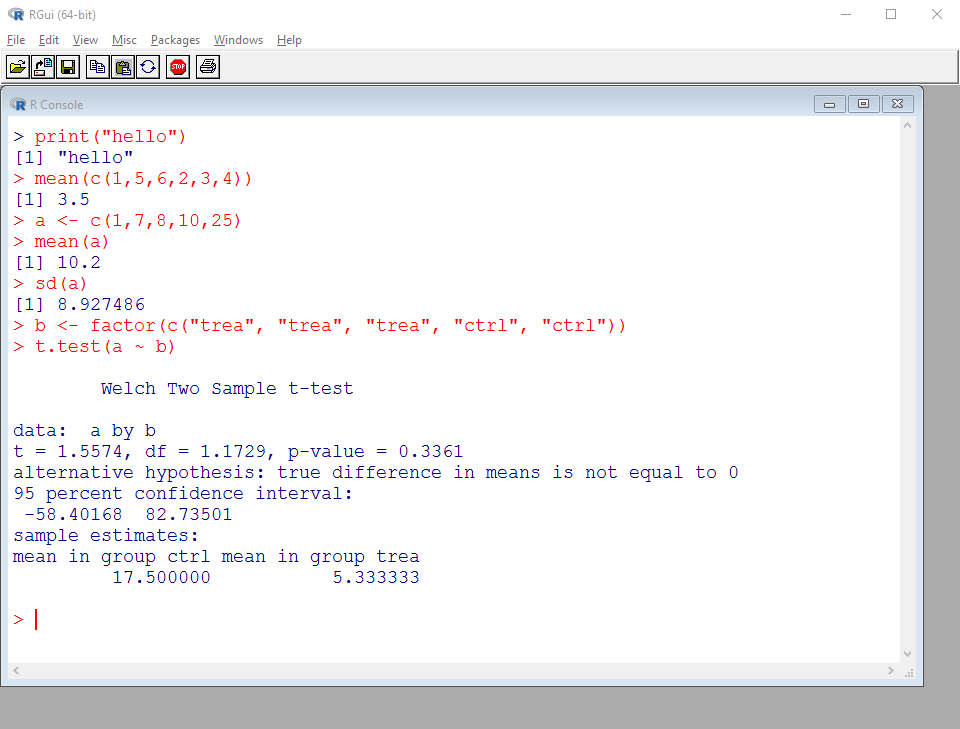
\includegraphics[width=0.85\textwidth]{figures/R-console-capture}
  \caption[Screen capture of the R console]{Screen capture of the R console being used interactively. Commands entered by the user is displayed in red, while the result returned by R is displayed in blue.}\label{fig:intro:console}
\end{figure}

\subsubsection{Using R as a ``batch job''}

To run a script we need first to prepare a script in a text editor. Figure \ref{fig:intro:script} shows the console immediately after running the script file shown in the lower window. As before, red text, the command \code{source("my-script.R")}, was typed by the user, and the blue text in the console is what was displayed by R as a result of this action.

\begin{figure}
  \centering
  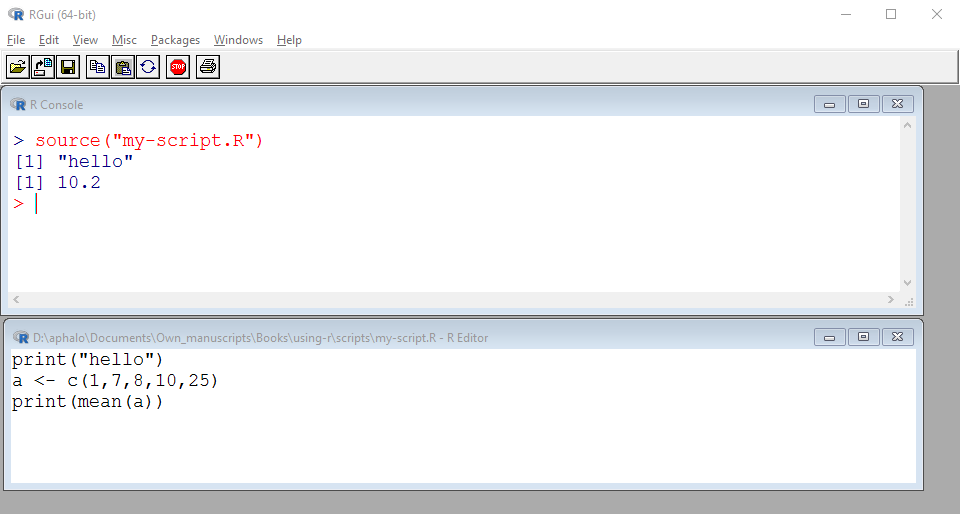
\includegraphics[width=0.85\textwidth]{figures/R-console-script}
  \caption[Script sourced at the R console]{Screen capture of the R console and editor just after running a script. The upper window shows the R console, and the lower window the script file in an editor window. }\label{fig:intro:script}
\end{figure}

A true ``batch job'' is not run at the R console but at the operating system command prompt, or shell. The shell is the console of the operating system---Linux, Unix, OS X, or MS-Windows. Figure \ref{fig:intro:shell} shows how running an script at the Windows commands prompt looks. In normal use, a script run at the operating system prompt does time-consuming calculations and the output is saved to a file. One may use this approach on a server, say, to leave the batch job running over-night.

\begin{figure}
  \centering
  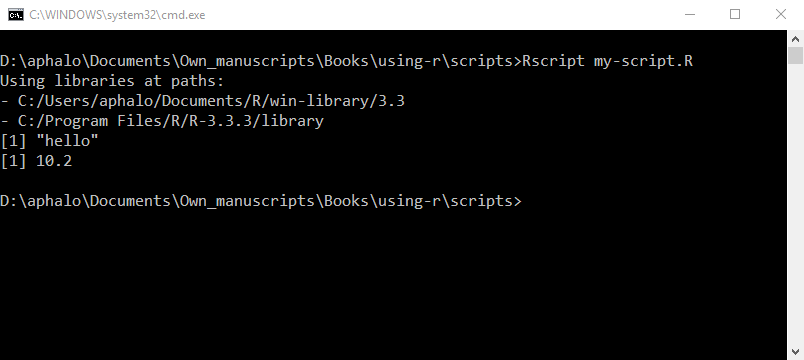
\includegraphics[width=0.85\textwidth]{figures/windows-cmd-script}
  \caption[Script at the Windows cmd promt]{Screen capture Windows 10 command console just after running the same script. Here we use \code{Rscript} to run the script, the exact syntax will depend on the operating system in use. In this case R prints the results at the operating system console or shell, rather than in its own R console.}\label{fig:intro:shell}
\end{figure}

\subsubsection{Editors and IDEs}

Integrated Development Environments (IDEs) were initially created for computer program development. They are programs that the user interacts with, from within which the different tools needed can be used in a coordinated way. They usually include a dedicated editor capable of displaying the output from different tools in a useful way, and also in many cases can do syntax highlighting, and even report some mistakes, related to the programming language in use while the user types. One could describe such editor as the equivalent as a word processor, that can check the program code for spelling and syntax errors, and has a built-in thesaurus for the computer language. In the case of RStudio, the main, but not only language supported is \Rlang. The main window of IDEs usually displays several panes simultaneously. From within the IDE one has access to the R console, an editor, a file-system browser, and access to several tools. Although RStudio supports very well the development of large scripts and packages, it is also the best possible way of using R at the console as it has the R help system very well integrated. Figure \ref{fig:intro:rstudio} shows the window displayed by RStudio under Windows after running the same script as shown above at the R console and at the operating system command prompt. We can see in this figure how RStudio is really a layer between the user and an unmodified R executable. The script was sourced by pressing the ``Source'' button at the top of the editor pane. RStudio in response to this generated the code needed to source the file and ``entered'' it at the console, the same console, where we would type ourselves any R commands.

\begin{figure}
  \centering
  \includegraphics[width=0.99\textwidth]{figures/Rstudio-script}
  \caption[Script in Rstudio]{The RStudio interface just after running the same script. Here we used the ``Source'' button to run the script. In this case R prints the results to the R console in the lower left pane.}\label{fig:intro:rstudio}
\end{figure}

When a script is run, if an error is triggered, it automatically finds the location of the error. \RStudio also supports the concept of projects allowing saving of settings per project. Some features are beyond what you need for everyday data analysis and aimed at package development, such as integration of debugging, traceback on errors, profiling and bench marking of code so as to analyse and improve performance. It also integrates support for file version control, which is not only useful for package development, but also for keeping track of the progress or collaboration in the analysis of data.

The version of RStudio that one uses locally, i.e.\ installed in your own computer, runs with almost identical user interface on most modern operating systems, such as Linux, Unix, OS X, and MS-Windows. There is also a server version that runs on Linux, and that can be used remotely through any web browser. The user interface is still the same.

\RStudio is under active development, and constantly improved. Visit \url{http://www.rstudio.org/} for an up-to-date description and download and installation instructions. Two books \autocite{vanderLoo2012,Hillebrand2015} describe and teach how to use \RStudio without going in depth into data analysis or statistics, however, as \RStudio is under very active development several recently added important features are not described in these books. You will find tutorials and up-to-date cheat sheets at \url{http://www.rstudio.org/}.

\section{Packages and repositories}

The most elegant way of adding new features or capabilities to \Rlang is through packages. This is without doubt the best mechanism when these extensions to R need to be shared. However, in most situations it is also the best mechanism for managing code that will be reused even by a single person over time. R packages have strict rules about their contents, file structure, and documentation, which makes it possible among other things for the package documentation to be merged into R's help system when a package is loaded. With a few exceptions, packages can be written so that they will work on any computer where R runs.

Packages can be shared as source or binary package files, sent for example through e-mail. However, for sharing packages widely, best is to submit them to a repository. The largest public repository of R packages is called CRAN, an acronym for Comprehensive R Archive Network. Packages available through CRAN are guaranteed to work, in the sense of not failing any tests built into the package and not crashing or aborting prematurely. They are tested daily, as they may depend on other packages whose code will change when updated. In January 2017, the number of packages available through CRAN passed the 10\,000 mark.

\section{Reproducible data analysis}

One requirement for reproducible data analysis, is a reliable record of what commands have been run on which data. Such a record is specially difficult to keep when issuing commands through menus and dialogue boxes in a graphical user interface. When working interactively at the R console, it is a bit easier, but still copying and pasting is error prone.

A further requirement is to be able to match the output of the R commands to the output. If the script generates the output to separate files, then the user will need to take care that the script saved or shared as record of the data analysis was the one actually used for obtaining the reported results and conclusions. This is another error prone stage in the report of a data analysis. To solve this problem an approach was developed, inspired in what is called \emph{literate programming} \autocite{Knuth1984a}. The idea is that running the script will produce a document that includes the script, the results of running the scripts and any explanatory text needed to understand and interpret the analysis.

Although a system capable of producing such reports, called \pkgname{Sweave} \autocite{Leisch2002}, has been available for a couple decades, it was rather limited and not supported by an IDE, making its use rather tedious. A more recently developed system called \pkgname{knitr} \autocite{Xie2013} together with its integration into RStudio has made the use of this type of reports very easy. The most recent development are Notebooks produced within RStudio. This very new feature, can produce the readable report of running the script, including the code used interspersed with the results within the viewable file. However, this newer approach goes even further: the actual source script used to generate the report is embedded in the HTML file of the report. This means that anyone who gets access to the output of the analysis in human readable form also gets access to the code used to generate the report, in computer executable format.

Because of these recent developments, R is an ideal language to use when the goal of reproducibility is important. During recent years the problem of the lack of reproducibility in scientific research has been broadly discussed and analysed \autocite{Gandrud2015}. One on the problems faced when attempting to reproduce experimental work, is reproducing the data analysis. R together with these modern tools can help in avoiding this source of lack of reproducibility.

How powerful are these tools? and how flexible? They are powerful and flexible enough to write whole books, such as this very book you are now reading, produced with R, knitr and \LaTeX. All pages in the book are generated directly, all figures are generated by R and included automatically, except for the figures in this chapter that have been manually captured from the computer screen. Why am I using this approach? First because I want to make sure that every bit of code as you will see printed, runs without error. In addition I want to make sure that the output that you will see below every line or chunk of R language code is exactly what R returns. Furthermore, it saves a lot of work for me as author, as I can just update R and all the packages used to their latest version, and build the book again, to keep it up to date and free of errors.

Although the use of these tools is important, they are outside the scope of this book. Still when writing code, using a consistent style for formatting and indentation, carefully choosing variable names, and adding textual explanations in comments when needed, helps very much with readability for humans. I have tried to be as consistent as possible throughout the whole book in this respect, with only small personal deviations from the usual style.

\section{Finding additional information}

When searching for answers, asking for advice or reading books you will be confronted with different ways of doing the same tasks. Do not allow this overwhelm you, in most cases it will not matter as many computations can be done in \Rpgrm, as in any language, in several different ways, still obtaining the same result. The different approaches may differ mainly in two aspects: 1) how readable to humans are the instructions given to the computer as part of a script or program, and 2) how fast the code runs. Unless performance is an important bottleneck in your work, just concentrate on writing code that is easy to understand to you and to others, and consequently easy to check and reuse. Of course do always check any code you write for mistakes, preferably using actual numerical test cases for any complex calculation or even relatively simple scripts. Testing and validation are extremely important steps in data analysis, so get into this habit while reading this book. Testing how every function works as I will challenge you to do in this book, is at the core of any robust data analysis or computing programming. When developing R packages, including a good coverage of test cases as part of the package itself simplifies code maintenance enormously, helps in maintaining consistency of behaviour across versions.

\subsection{R's built-in help}

To\index{R!help} access help pages through the command prompt we use function \texttt{help()} or a question mark. Every object exported by an R package (functions, methods, classes, data) is documented. Sometimes a single help page documents several R objects. Usually at the end of the help pages, some examples are given, which tend to help very much in learning how to use the functions described. For example one can search for a help page at the R console.

\begin{knitrout}\footnotesize
\definecolor{shadecolor}{rgb}{0.969, 0.969, 0.969}\color{fgcolor}\begin{kframe}
\begin{alltt}
\hlkwd{help}\hlstd{(}\hlstr{"sum"}\hlstd{)}
\hlopt{?}\hlstd{sum}
\end{alltt}
\end{kframe}
\end{knitrout}

\begin{playground}
Look at help for some other functions like \code{mean()}, \code{var()}, \code{plot()} and, why not, \code{help()} itself!
\begin{knitrout}\footnotesize
\definecolor{shadecolor}{rgb}{0.969, 0.969, 0.969}\color{fgcolor}\begin{kframe}
\begin{alltt}
\hlkwd{help}\hlstd{(help)}
\end{alltt}
\end{kframe}
\end{knitrout}
\end{playground}

When using \RStudio there are several easier ways of navigating to a help page, for example with the cursor on the name of a function in the editor or console, pressing the F1 key, opens the corresponding help page in the help pane. Letting the cursor hover for a few seconds over the name of a function at the R console will open ``bubble help'' for it. If the function is defined in a script or another file open in the editor pane one can directly navigate from the line where the function is called to where it is defined. In RStudio one can also search for help through the graphical interface.

In addition to help pages, the \pgrmname{R}'s distribution includes useful manuals as PDF or HTML files. This can be accessed most easily through the Help menu in \RStudio or \pgrmname{RGUI}. Extension packages, provide help pages for the functions and data they export. When a package is loaded into an \pgrmname{R} session, its help pages are added to the native help of \pgrmname{R}. In addition to these individual help pages, each package, provides an index of its corresponding help pages, for users to browse. Many packages, also provide \emph{vignettes} such as User Guides or articles describing the algorithms used.

There are some web sites that give access to R documentation through a web server. These sites can be very convenient when exploring whether a certain package could be useful for a certain problem, as they allow browsing and searching the documentation without need of installing the packages. Some package maintainers have web sites with additional documentation for their own packages. The DESCRIPTION or README of packages provide contact information for the maintainer, links to web sites, and instructions on how to report bugs.

\subsection{Obtaining help from on-line forums}

\subsubsection{Netiquette}
In\index{netiquette}\index{network etiquette} most internet forums, a certain behaviour is expected from those asking and answering questions. Some types of miss-behavior, like use of offensive or inappropriate language, will usually result in the user being banned writing rights in a forum. Occasional minor miss-behaviour, will usually result in the original question not being answered and instead the problem highlighted in the reply.

\begin{itemize}
  \item Do your homework: first search for existing answers to your question, both on-line and in the documentation. (Do mention that you attempted this without success when you post your question.)
  \item Provide a clear explanation of the problem, and all the relevant information. Say if it concerns R, the version, operating system, and any packages loaded and their versions.
  \item If at all possible provide a simplified and short, but self-contained, code example that reproduces the problem (sometimes called \emph{reprex}).
  \item Be polite.
  \item Contribute to the forum by answering other users' questions when you know the answer.
\end{itemize}

\begin{explainbox}
 How to prepare a reproducible example (reprex).
\end{explainbox}

\subsubsection{StackOverflow}

Nowadays, StackOverflow (\url{http://stackoverflow.com/})\index{StackOverflow} is the best questions and answers (Q\,\&\,A)support site for \pgrmname{R}. In most cases, searching for existing questions and their answers, will be all what you need to do. If asking a question, make sure that it is really a new question. If there is some question that looks similar, make clear how your question is different.

StackOverflow has a user-rights system based on reputation, and questions and answers can be up- and down-voted. Those with the most up-votes are listed at the top of searches. If the questions or answers you write are up-voted after you accumulate enough reputation you acquire badges, and rights, such as editing other users' questions and answers or later on, even deleting wrong answers or off-topic questions from the system. This sounds complicated, but works extremely well at ensuring that the base of questions and answers is relevant and correct, without relying on a single or ad-hoc \emph{moderators}.

\section{What is needed to run the examples on this book?}

The book is written with the expectation that you will run most of the code examples and try as many other variations as needed until you are sure to understand the basic `rules' of the \Rpgrm language and how each function or command described works. In \Rpgrm for each function, data set, etc.\ there is a help page available. Error messages tend to be terse in \Rpgrm, and may require some lateral thinking and/or `experimentation' to understand the real cause behind problems. When you are not sure to understand how some command works, it is useful in many cases to try simple examples for which you know the correct answer and see if you can reproduce them with \Rpgrm. Because of this, this book also includes some code examples that trigger errors. To test your understanding of how a code statement or function works, it is good to try your hand at testing its limits, testing which variations of a piece code are valid or not.

I recommend you to use as an editor or IDE (integrated development environment) \RStudio. \RStudio is user friendly, actively maintained, free, open-source and available both in desktop and server versions. The desktop version runs on Windows, Linux, and OS X and other Unixes. For\index{IDE for R}\index{editor for R scripts} running the examples in the handbook, you would need only to have \pgrmname{R} installed. That would be enough as long as you also have a text editor available. This is possible, but does not give a very smooth work flow for data analyses that are beyond the very simple. The next stage is to use a text editor which integrates to some extent with R, but still this is not ideal, specially for writing packages or long scripts for data analysis. Currently, by far the best option is to use \RStudio.

Of course when choosing which editor to use, personal preferences and previous familiarity play an important.
Currently, for the development of packages, I use \RStudio exclusively. For writing this book I have used both RStudio and the text editor WinEdt which also has some support for R together with excellent support for \LaTeX. When working on a large project or collaborating with other data analysts or researchers, one big advantage of a system based on plain text files, is that the same files can be edited with different programs as needed or wished by the different persons involved in a project.

When I started using R, nearly two decades ago, I was using other editors, using the operating system shell a lot more, and struggling with debugging as no IDE was available. The only reasonably good integration with an editor was for Emacs, which was widely available only under Unix-like systems. Given this past experience, I encourage you to use an IDE for R. \RStudio is nowadays very popular, but if you do not like it, need a different set of features, such as integration with \pgrmname{ImageJ}, or are already familiar with the \pgrmname{Eclipse} IDE, you may like try the \pgrmname{Bio7} IDE, available from \url{http://bio7.org}.

The examples make use of several freely available packages, with can be obtained installed from CRAN. One of them \pkgname{learnrbook} also available through CRAN, contains data sets and files specific to this book. The \pkgname{learnrbook} package also contains installation instructions and saved lists of the names of all other packages used in the book. Instructions on installing R, Git, RStudio, compilers and other tools are available on-line. In many cases the IT staff at your employer or school will know how to install them, or they may be even included in the default computer setup. In addition a web site supporting the book is available at: \url{http://www.learnr-book.info}.

\section{Working at the R console}
\index{console}
The examples in the book use only the console window for user input. Menu-driven programs are not necessarily bad, they are just unsuitable when there is a need to set very many options and choose from many different actions. They are also difficult to maintain when extensibility is desired, and when independently developed modules of very different characteristics need to be integrated. Textual languages also have the advantage, to be dealt in later chapters, that command sequences can be stored in human- and computer readable text files. Such files constitute a record of all the steps used and in most cases makes it trivial to reproduce the same steps at a later time. Scripts are also a very simple and handy way of communicating to others how to do a given data analysis.

In the console you can type commands at the \code{>} prompt.
When you end a line by pressing the return key, if the line can be interpreted as an R command, the result will be printed at the console, followed by a new \code{>} prompt.
If the command is incomplete a \code{+} continuation prompt will be shown, and you will be able to type-in the rest of the command. For example if the whole calculation that you would like to do is $1 + 2 + 3$, if you enter in the console \code{1 + 2 +} in one line, you will get a continuation prompt where you will be able to type \code{3}. However, if you type \code{1 + 2}, the result will be calculated, and printed.

When working at the command prompt, most results are printed by default, but in other cases you may need to use the function \Rfunction{print()} explicitly. Most examples in the book rely on automatic printing of output. To effectively learn from this book, you will need to work your way through the code examples. This book's approach is that of a travel-guide, it aims at helping you find your own way in the world of R. Your travels in the world of \Rlang will start on the next page. Enjoy them!





% !Rnw root = appendix.main.Rnw



\chapter{The R language: ``words'' and ``sentences''}\label{chap:R:as:calc}

\begin{VF}
The desire to economize time and mental effort in arithmetical computations, and to eliminate human liability to error, is probably as old as the science of arithmetic itself.

\VA{Howard Aiken}{Proposed automatic calculating machine}
\end{VF}

%\dictum[Howard Aiken, \emph{Proposed automatic calculating machine}, presented to IBM in 1937]{The desire to economize time and mental effort in arithmetical computations, and to eliminate human liability to error, is probably as old as the science of arithmetic itself.}\vskip2ex

\section{Aims of this chapter}

In my experience, for those not familiar with computer programming languages, the best first step in learning \Rlang is to use it at the R command prompt by issuing textual commands. This will teach not only the syntax and grammar rules, but also give a glimpse at the advantages and flexibility of this approach to data analysis.

In the first part of the chapter we will use \Rlang to do everyday calculations that should be so easy and familiar that you will not need to think about the operations themselves. This easy start will give you a chance to focus on learning how to issue textual commands at the command prompt.

Later in the chapter, you will gradually need to focus more on the \Rlang language and less on how commands are entered. By the end of the chapter you will be familiar with most of the kinds of ``words'' used in the R language and you will be able write simple ``sentences''.

Along the chapter, I will show occasionally the equivalent of the R code in mathematical notation. If you are not familiar with the mathematical notation, you can safely ignore it, as long as you understand the \Rlang code.

\section{Natural and computer languages}

Computer languages have strict rules and interpreters and compilers are unforgiving about errors. They will issue error messages, but in contrast to human readers or listeners, will not guess your intentions and continue. However, computer languages have a much smaller set of words than natural languages, such as English. If you are new to computer programming, understanding the parallels between computer and natural languages may be useful.

One can think of constant values and variables (values stored under a name) as nouns and of operators and functions as verbs. A complete command, or statement, is the equivalent of a natural language sentence: ``a comprehensible utterance''. The simple statement \code{a + 1} has three components: \code{a}, a variable, \code{+}, an operator and \code{1} a constant. The statement \code{sqrt(4)} has two components, a function \code{sqrt()} and a numerical constant \code{4}. We say that ``to compute $\sqrt{4}$ we \emph{call} \code{sqrt()} with \code{4} as its \emph{argument}''.

In later chapters you will learn how to write compound statements, the equivalent of natural-language paragraphs, and scripts, the equivalent of essays. You will also learn how to define new verbs, user defined functions and operators, and new nouns, user defined classes.

\section{Arithmetic and numeric values}
\index{mode!numeric|(}\index{math operators}\index{math functions}\index{numeric values}
When working in \Rlang with arithmetic expressions, the normal mathematical precedence rules are respected, but parentheses can be used to alter this order. Parentheses can be nested, but in contrast to the usual practice in mathematics, the same parenthesis symbol is used at all nesting levels.

The equivalent of the math expression
$$
\frac{3 + e^2}{\sin \pi}
$$
is
\begin{knitrout}\footnotesize
\definecolor{shadecolor}{rgb}{0.969, 0.969, 0.969}\color{fgcolor}\begin{kframe}
\begin{alltt}
\hlstd{(}\hlnum{3} \hlopt{+} \hlkwd{exp}\hlstd{(}\hlnum{2}\hlstd{))} \hlopt{/} \hlkwd{sin}\hlstd{(pi)}
\end{alltt}
\begin{verbatim}
## [1] 8.483588e+16
\end{verbatim}
\end{kframe}
\end{knitrout}

It can be seen above that mathematical constants and functions are part of the \Rlang language. One thing to remember when translating complex fractions as above into R code, is that the bar in the fraction generates a grouping that alters the normal precedence, requiring additional parentheses in the \Rlang version.

If you are in doubt about how precedence rules work, you can add parentheses to make sure the order of computations is the one you intend.

\begin{knitrout}\footnotesize
\definecolor{shadecolor}{rgb}{0.969, 0.969, 0.969}\color{fgcolor}\begin{kframe}
\begin{alltt}
\hlnum{1} \hlopt{+} \hlnum{2} \hlopt{*} \hlnum{3}
\end{alltt}
\begin{verbatim}
## [1] 7
\end{verbatim}
\begin{alltt}
\hlnum{1} \hlopt{+} \hlstd{(}\hlnum{2} \hlopt{*} \hlnum{3}\hlstd{)}
\end{alltt}
\begin{verbatim}
## [1] 7
\end{verbatim}
\begin{alltt}
\hlstd{(}\hlnum{1} \hlopt{+} \hlnum{2}\hlstd{)} \hlopt{*} \hlnum{3}
\end{alltt}
\begin{verbatim}
## [1] 9
\end{verbatim}
\end{kframe}
\end{knitrout}

The number of opening (left side) and closing (right side) parentheses must be balanced, and they must be located so that each enclosed term is a valid mathematical expression. For example while \code{(1 + 2) * 3} is valid, \code{(1 +) 2 * 3} is a syntax error as \code{1 +} is incomplete and cannot be calculated.

\begin{playground}
Here results are not shown. These are examples for you to type at the command prompt. In general you should not skip them, as in many cases, as with the statements highlighted with comments in the code chunk below, they have something to teach or demonstrate. You are also strongly encouraged to \emph{play}, in other words, create new variations of the examples and execute them to explore how \Rlang works.

\begin{knitrout}\footnotesize
\definecolor{shadecolor}{rgb}{0.969, 0.969, 0.969}\color{fgcolor}\begin{kframe}
\begin{alltt}
\hlnum{1} \hlopt{+} \hlnum{1}
\hlnum{2} \hlopt{*} \hlnum{2}
\hlnum{2} \hlopt{+} \hlnum{10} \hlopt{/} \hlnum{5}
\hlstd{(}\hlnum{2} \hlopt{+} \hlnum{10}\hlstd{)} \hlopt{/} \hlnum{5}
\hlnum{10}\hlopt{^}\hlnum{2} \hlopt{+} \hlnum{1}
\hlkwd{sqrt}\hlstd{(}\hlnum{9}\hlstd{)}
\hlstd{pi} \hlcom{# whole precision not shown when printing}
\hlkwd{print}\hlstd{(pi,} \hlkwc{digits} \hlstd{=} \hlnum{22}\hlstd{)}
\hlkwd{sin}\hlstd{(pi)} \hlcom{# oops! Read on for explanation.}
\hlkwd{log}\hlstd{(}\hlnum{100}\hlstd{)}
\hlkwd{log10}\hlstd{(}\hlnum{100}\hlstd{)}
\hlkwd{log2}\hlstd{(}\hlnum{8}\hlstd{)}
\hlkwd{exp}\hlstd{(}\hlnum{1}\hlstd{)}
\end{alltt}
\end{kframe}
\end{knitrout}

\end{playground}

Variables\index{variables}\index{assignment} are used to store values. The `usual' assignment operator is \Roperator{<-}. All names in \Rlang are case sensitive. Variables \code{a} and \code{A} are two different variables. Variable names can be quite long, but usually it is not a good idea to use very long names. Here I am using very short names, something that is usually a very bad idea. However, in the examples in this chapter where the stored values have no connection to the real world, simple names emphasize their abstract nature.

\begin{knitrout}\footnotesize
\definecolor{shadecolor}{rgb}{0.969, 0.969, 0.969}\color{fgcolor}\begin{kframe}
\begin{alltt}
\hlstd{a} \hlkwb{<-} \hlnum{1}
\hlstd{a} \hlopt{+} \hlnum{1}
\end{alltt}
\begin{verbatim}
## [1] 2
\end{verbatim}
\begin{alltt}
\hlstd{a}
\end{alltt}
\begin{verbatim}
## [1] 1
\end{verbatim}
\begin{alltt}
\hlstd{b} \hlkwb{<-} \hlnum{10}
\hlstd{b} \hlkwb{<-} \hlstd{a} \hlopt{+} \hlstd{b}
\hlstd{b}
\end{alltt}
\begin{verbatim}
## [1] 11
\end{verbatim}
\begin{alltt}
\hlnum{3e-2} \hlopt{*} \hlnum{2.0}
\end{alltt}
\begin{verbatim}
## [1] 0.06
\end{verbatim}
\end{kframe}
\end{knitrout}

\begin{playground}
There are some syntactically legal statements that are not very frequently used, but you should be aware that they are valid, as they will not trigger error messages, and may surprise you. The most important thing is to write code consistently. The `backwards' assignment operator \Roperator{->} and resulting code like \code{1 -> a}\index{assignment!leftwise} are valid but less frequently used. The use of the equals sign (\Roperator{=}) for assignment in place of \Roperator{->} although valid is generally discouraged as this redundant use was not part of the \Rlang language as originally defined. Chaining\index{assignment!chaining} assignments as in the first line below is sometimes used, and signals to the human reader that \code{a}, \code{b} and \code{c} are being assigned the same value.

\begin{knitrout}\footnotesize
\definecolor{shadecolor}{rgb}{0.969, 0.969, 0.969}\color{fgcolor}\begin{kframe}
\begin{alltt}
\hlstd{a} \hlkwb{<-} \hlstd{b} \hlkwb{<-} \hlstd{c} \hlkwb{<-} \hlnum{0.0}
\hlstd{a}
\hlstd{b}
\hlstd{c}
\hlnum{1} \hlkwb{->} \hlstd{a}
\hlstd{a}
\hlstd{a} \hlkwb{=} \hlnum{3}
\hlstd{a}
\end{alltt}
\end{kframe}
\end{knitrout}

\end{playground}

\begin{explainbox}
Here I very briefly introduce the concept of \emph{mode} of an R object. In the case of \Rlang, numbers, belong to mode \Rclass{numeric}. We can query if the mode of an object is \Rclass{numeric} with function \Rfunction{is.numeric()}.

\begin{knitrout}\footnotesize
\definecolor{shadecolor}{rgb}{0.969, 0.969, 0.969}\color{fgcolor}\begin{kframe}
\begin{alltt}
\hlkwd{mode}\hlstd{(}\hlnum{1}\hlstd{)}
\end{alltt}
\begin{verbatim}
## [1] "numeric"
\end{verbatim}
\begin{alltt}
\hlstd{a} \hlkwb{<-} \hlnum{1}
\hlkwd{mode}\hlstd{(a)}
\end{alltt}
\begin{verbatim}
## [1] "numeric"
\end{verbatim}
\begin{alltt}
\hlkwd{is.numeric}\hlstd{(a)}
\end{alltt}
\begin{verbatim}
## [1] TRUE
\end{verbatim}
\end{kframe}
\end{knitrout}

One can think informally of a \emph{mode}, as a ``type'' or ``kind'' of objects. Constants like \code{1} or variables such as \code{a} in the code chunk above, belong to, or have a mode, that indicates that they are numbers. Other modes that we will use later in the present chapter are \code{logical} and \code{character} (We will discuss the concepts of \emph{mode} and \emph{class}, as used in \langname{R}, in section \ref{sec:rlang:mode} on page \pageref{sec:rlang:mode}).

As in computers numbers can be stored in different formats requiring different amounts of memory, most computing languages implement several different types of numbers. In most cases \Rpgrm's \Rfunction{numeric()} can be used everywhere where a number is expected. In some cases it can be more efficient to explicitly indicate whether we will store or operate on integer numbers, in which case we can use class \Rclass{integer}, with integer constants indicated with a trailing capital `L', as in  \code{32L}.

Real numbers are a mathematical abstraction, and do not have an exact equivalent in computers. Instead of Real numbers, computers store and operate on numbers that are restricted to a broad but finite range values and have a finite resolution. They are called, \emph{floats} (or \emph{floating-point} numbers), in R they go by the name of \Rclass{double} and can be created with the constructor \Rfunction{double()}.

\begin{knitrout}\footnotesize
\definecolor{shadecolor}{rgb}{0.969, 0.969, 0.969}\color{fgcolor}\begin{kframe}
\begin{alltt}
\hlkwd{is.numeric}\hlstd{(}\hlnum{1L}\hlstd{)}
\end{alltt}
\begin{verbatim}
## [1] TRUE
\end{verbatim}
\begin{alltt}
\hlkwd{is.integer}\hlstd{(}\hlnum{1L}\hlstd{)}
\end{alltt}
\begin{verbatim}
## [1] TRUE
\end{verbatim}
\begin{alltt}
\hlkwd{is.double}\hlstd{(}\hlnum{1L}\hlstd{)}
\end{alltt}
\begin{verbatim}
## [1] FALSE
\end{verbatim}
\end{kframe}
\end{knitrout}

The name \code{double} originates from the \pgrmname{C} language, in which there are different types of floats available. With the word \code{double} used to mean ``double-precision floating-point numbers''. Similarly, the use of \code{L} stems the \texttt{long} type in \pgrmname{C}, meaning ``long integer numbers''.
\end{explainbox}

Numeric variables can contain more than one value. Even single numbers are in \langname{R} \Rclass{vector}s of length one. We will later see why this is important. As you have seen above, the results of calculations were printed preceded with \code{[1]}. This is the index or position in the vector of the first number (or other value) displayed at the head of the current line.

One can use \Rmethod{c()} `concatenate' to create a vector from other vectors, including vectors of length 1, such as the \code{numeric} constants in the statements below.

\begin{knitrout}\footnotesize
\definecolor{shadecolor}{rgb}{0.969, 0.969, 0.969}\color{fgcolor}\begin{kframe}
\begin{alltt}
\hlstd{a} \hlkwb{<-} \hlkwd{c}\hlstd{(}\hlnum{3}\hlstd{,} \hlnum{1}\hlstd{,} \hlnum{2}\hlstd{)}
\hlstd{a}
\end{alltt}
\begin{verbatim}
## [1] 3 1 2
\end{verbatim}
\begin{alltt}
\hlstd{b} \hlkwb{<-} \hlkwd{c}\hlstd{(}\hlnum{4}\hlstd{,} \hlnum{5}\hlstd{,} \hlnum{0}\hlstd{)}
\hlstd{b}
\end{alltt}
\begin{verbatim}
## [1] 4 5 0
\end{verbatim}
\begin{alltt}
\hlstd{c} \hlkwb{<-} \hlkwd{c}\hlstd{(a, b)}
\hlstd{c}
\end{alltt}
\begin{verbatim}
## [1] 3 1 2 4 5 0
\end{verbatim}
\begin{alltt}
\hlstd{d} \hlkwb{<-} \hlkwd{c}\hlstd{(b, a)}
\hlstd{d}
\end{alltt}
\begin{verbatim}
## [1] 4 5 0 3 1 2
\end{verbatim}
\end{kframe}
\end{knitrout}

Method \code{c()} accepts as argument two or more vectors and concatenates them, one after another. Quite frequently we may need to insert one vector in the middle of another. For this operation, \code{c()} is not useful by itself. One could use indexing combined with \code{c()}, but this is not needed as R provides a function capable of directly doing this operation. Although it can be used to ``insert'' values it is named \code{append()}, and by default, it indeed appends one vector at the end of another.

\begin{knitrout}\footnotesize
\definecolor{shadecolor}{rgb}{0.969, 0.969, 0.969}\color{fgcolor}\begin{kframe}
\begin{alltt}
\hlkwd{append}\hlstd{(a, b)}
\end{alltt}
\begin{verbatim}
## [1] 3 1 2 4 5 0
\end{verbatim}
\end{kframe}
\end{knitrout}

The output above is the same as for \code{c(a, b)}, however, \code{append()} accepts as argument an index position after which to ``append'' its second argument. This results in an \emph{insert} operation when the index points at any position different from the end of the vector.

\begin{knitrout}\footnotesize
\definecolor{shadecolor}{rgb}{0.969, 0.969, 0.969}\color{fgcolor}\begin{kframe}
\begin{alltt}
\hlkwd{append}\hlstd{(a,} \hlkwc{values} \hlstd{= b,} \hlkwc{after} \hlstd{=} \hlnum{2L}\hlstd{)}
\end{alltt}
\begin{verbatim}
## [1] 3 1 4 5 0 2
\end{verbatim}
\end{kframe}
\end{knitrout}

Both \code{c()} and \code{append()} can be also used with lists.

\begin{playground}
One can create sequences\index{sequence} using function \Rfunction{seq()} or the operator \Roperator{:}, or repeat values using function \Rfunction{rep()}. In this case I leave to the reader to work out the rules by running these and his/her own examples, with the help of the documentation, available through \code{help(seq)} and \code{help(rep)}.

\begin{knitrout}\footnotesize
\definecolor{shadecolor}{rgb}{0.969, 0.969, 0.969}\color{fgcolor}\begin{kframe}
\begin{alltt}
\hlstd{a} \hlkwb{<-} \hlopt{-}\hlnum{1}\hlopt{:}\hlnum{5}
\hlstd{a}
\hlstd{b} \hlkwb{<-} \hlnum{5}\hlopt{:-}\hlnum{1}
\hlstd{b}
\hlstd{c} \hlkwb{<-} \hlkwd{seq}\hlstd{(}\hlkwc{from} \hlstd{=} \hlopt{-}\hlnum{1}\hlstd{,} \hlkwc{to} \hlstd{=} \hlnum{1}\hlstd{,} \hlkwc{by} \hlstd{=} \hlnum{0.1}\hlstd{)}
\hlstd{c}
\hlstd{d} \hlkwb{<-} \hlkwd{rep}\hlstd{(}\hlopt{-}\hlnum{5}\hlstd{,} \hlnum{4}\hlstd{)}
\hlstd{d}
\end{alltt}
\end{kframe}
\end{knitrout}

\end{playground}

Next something that makes \Rlang different from most other programming languages: vectorized arithmetic\index{vectorized arithmetic}. Operators and functions that are vectorized accept as argument vectors of arbitrary length, in which case the result returned is equivalent to having applied the same function or operator to each element of the vector individually.\label{par:vectorized:numeric}

\begin{knitrout}\footnotesize
\definecolor{shadecolor}{rgb}{0.969, 0.969, 0.969}\color{fgcolor}\begin{kframe}
\begin{alltt}
\hlstd{a} \hlopt{+} \hlnum{1} \hlcom{# we add one to vector a defined above}
\end{alltt}
\begin{verbatim}
## [1] 4 2 3
\end{verbatim}
\begin{alltt}
\hlstd{(a} \hlopt{+} \hlnum{1}\hlstd{)} \hlopt{*} \hlnum{2}
\end{alltt}
\begin{verbatim}
## [1] 8 4 6
\end{verbatim}
\begin{alltt}
\hlstd{a} \hlopt{+} \hlstd{b}
\end{alltt}
\begin{verbatim}
## [1] 7 6 2
\end{verbatim}
\begin{alltt}
\hlstd{a} \hlopt{-} \hlstd{a}
\end{alltt}
\begin{verbatim}
## [1] 0 0 0
\end{verbatim}
\end{kframe}
\end{knitrout}

As it can be seen in the first line above, another peculiarity of \Rpgrm, is what is frequently called ``recycling'' of arguments:\index{recycling@recycling of arguments} as vector \code{a} is of length 6, but the constant 1 is a vector of length 1, this 1 is extended by recycling into a vector of ones of the same length as the longest vector in the statement, in this case, \code{a}.\label{par:recycling:numeric}

Make sure you understand what calculations are taking place in the chunk above, and also the one below.

\begin{knitrout}\footnotesize
\definecolor{shadecolor}{rgb}{0.969, 0.969, 0.969}\color{fgcolor}\begin{kframe}
\begin{alltt}
\hlstd{a} \hlkwb{<-} \hlkwd{rep}\hlstd{(}\hlnum{1}\hlstd{,} \hlnum{6}\hlstd{)}
\hlstd{a}
\end{alltt}
\begin{verbatim}
## [1] 1 1 1 1 1 1
\end{verbatim}
\begin{alltt}
\hlstd{a} \hlopt{+} \hlnum{1}\hlopt{:}\hlnum{2}
\end{alltt}
\begin{verbatim}
## [1] 2 3 2 3 2 3
\end{verbatim}
\begin{alltt}
\hlstd{a} \hlopt{+} \hlnum{1}\hlopt{:}\hlnum{3}
\end{alltt}
\begin{verbatim}
## [1] 2 3 4 2 3 4
\end{verbatim}
\begin{alltt}
\hlstd{a} \hlopt{+} \hlnum{1}\hlopt{:}\hlnum{4}
\end{alltt}


{\ttfamily\noindent\color{warningcolor}{\#\# Warning in a + 1:4: longer object length is not a multiple of shorter object length}}\begin{verbatim}
## [1] 2 3 4 5 2 3
\end{verbatim}
\end{kframe}
\end{knitrout}

\begin{explainbox}
A useful thing to know: a vector can have length zero. Vectors of length zero may seem at first sight quite useless, but in fact they are very useful. They allow the handling of ``no input'' or ``nothing to do'' cases as normal cases, which in the absence of vectors of length zero would require to be treated as special cases. I describe here a useful function, \Rfunction{length()} which returns the length of a vector or list.

\begin{knitrout}\footnotesize
\definecolor{shadecolor}{rgb}{0.969, 0.969, 0.969}\color{fgcolor}\begin{kframe}
\begin{alltt}
\hlstd{z} \hlkwb{<-} \hlkwd{numeric}\hlstd{(}\hlnum{0}\hlstd{)}
\hlstd{z}
\end{alltt}
\begin{verbatim}
## numeric(0)
\end{verbatim}
\begin{alltt}
\hlkwd{length}\hlstd{(z)}
\end{alltt}
\begin{verbatim}
## [1] 0
\end{verbatim}
\end{kframe}
\end{knitrout}

Vectors and lists of length zero, behave in most cases, as expected---e.g.\ they can be concatenated as shown here.

\begin{knitrout}\footnotesize
\definecolor{shadecolor}{rgb}{0.969, 0.969, 0.969}\color{fgcolor}\begin{kframe}
\begin{alltt}
\hlkwd{length}\hlstd{(}\hlkwd{c}\hlstd{(a,} \hlkwd{numeric}\hlstd{(}\hlnum{0}\hlstd{), b))}
\end{alltt}
\begin{verbatim}
## [1] 9
\end{verbatim}
\begin{alltt}
\hlkwd{length}\hlstd{(}\hlkwd{c}\hlstd{(a, b))}
\end{alltt}
\begin{verbatim}
## [1] 9
\end{verbatim}
\end{kframe}
\end{knitrout}

Many functions, such as \Rlang's maths functions and operators, will accept numeric vectors of length zero as valid input, returning also a vector of length zero, issuing neither a warning nor an error message. In other words, \emph{these are valid operations} in \Rlang.

\begin{knitrout}\footnotesize
\definecolor{shadecolor}{rgb}{0.969, 0.969, 0.969}\color{fgcolor}\begin{kframe}
\begin{alltt}
\hlkwd{log}\hlstd{(}\hlkwd{numeric}\hlstd{(}\hlnum{0}\hlstd{))}
\end{alltt}
\begin{verbatim}
## numeric(0)
\end{verbatim}
\begin{alltt}
\hlnum{5} \hlopt{+} \hlkwd{numeric}\hlstd{(}\hlnum{0}\hlstd{)}
\end{alltt}
\begin{verbatim}
## numeric(0)
\end{verbatim}
\end{kframe}
\end{knitrout}

Even when of length zero, vectors do have to belong to a class acceptable for the operation.

\end{explainbox}

It is possible to \emph{remove} variables from the workspace with \Rfunction{rm()}. Function \Rfunction{ls()} returns a \emph{list} all objects in the current environment, or by supplying a \code{pattern} argument, only the objects with names matching the \code{pattern}. The pattern is given as a regular expression, with \verb|[]| enclosing alternative matching characters, \verb|^| and \verb|$| indicating the extremes of the name (start and end, respectively). For example \verb|"^z$"| matches only the single character `z' while \verb|"^z"| matches any name starting with `z'. In contrast \verb|"^[zy]$"| matches both `z' and `y' but neither `zy' nor `yz', and \verb|"^[a-z]"| matches any name starting with a lower case ASCII letter. If you are using \pgrmname{RStudio}, all objects are listed in the Environment pane, and the search box of the panel can be used to find a given object.

\begin{knitrout}\footnotesize
\definecolor{shadecolor}{rgb}{0.969, 0.969, 0.969}\color{fgcolor}\begin{kframe}
\begin{alltt}
\hlkwd{ls}\hlstd{(}\hlkwc{pattern}\hlstd{=}\hlstr{"^z$"}\hlstd{)}
\end{alltt}
\begin{verbatim}
## [1] "z"
\end{verbatim}
\begin{alltt}
\hlkwd{rm}\hlstd{(z)}
\hlkwd{ls}\hlstd{(}\hlkwc{pattern}\hlstd{=}\hlstr{"^z$"}\hlstd{)}
\end{alltt}
\begin{verbatim}
## character(0)
\end{verbatim}
\end{kframe}
\end{knitrout}

There are some special values available for numbers. \code{NA} meaning `not available' is used for missing values. Calculations can yield also the following values \code{NaN} `not a number', \code{Inf} and \code{-Inf} for $\infty$ and $-\infty$. As you will see below, calculations yielding these values do \textbf{not} trigger errors or warnings, as they are arithmetically valid. \code{Inf} and \code{-Inf} are also valid numerical values for input and constants.

\begin{knitrout}\footnotesize
\definecolor{shadecolor}{rgb}{0.969, 0.969, 0.969}\color{fgcolor}\begin{kframe}
\begin{alltt}
\hlstd{a} \hlkwb{<-} \hlnum{NA}
\hlstd{a}
\end{alltt}
\begin{verbatim}
## [1] NA
\end{verbatim}
\begin{alltt}
\hlopt{-}\hlnum{1} \hlopt{/} \hlnum{0}
\end{alltt}
\begin{verbatim}
## [1] -Inf
\end{verbatim}
\begin{alltt}
\hlnum{1} \hlopt{/} \hlnum{0}
\end{alltt}
\begin{verbatim}
## [1] Inf
\end{verbatim}
\begin{alltt}
\hlnum{Inf} \hlopt{/} \hlnum{Inf}
\end{alltt}
\begin{verbatim}
## [1] NaN
\end{verbatim}
\begin{alltt}
\hlnum{Inf} \hlopt{+} \hlnum{4}
\end{alltt}
\begin{verbatim}
## [1] Inf
\end{verbatim}
\begin{alltt}
\hlstd{b} \hlkwb{<-} \hlopt{-}\hlnum{Inf}
\hlstd{b} \hlopt{* -}\hlnum{1}
\end{alltt}
\begin{verbatim}
## [1] Inf
\end{verbatim}
\end{kframe}
\end{knitrout}

Not available (\code{NA}) values are very important in the analysis of experimental data, as frequently some observations are missing from an otherwise complete data set due to ``accidents'' during the course of an experiment. It is important to understand how to interpret \code{NA}'s. They are simple place holders for something that is unavailable, in other words \emph{unknown}.

\begin{knitrout}\footnotesize
\definecolor{shadecolor}{rgb}{0.969, 0.969, 0.969}\color{fgcolor}\begin{kframe}
\begin{alltt}
\hlstd{A} \hlkwb{<-} \hlnum{NA}
\hlstd{A}
\end{alltt}
\begin{verbatim}
## [1] NA
\end{verbatim}
\begin{alltt}
\hlstd{A} \hlopt{+} \hlnum{1}
\end{alltt}
\begin{verbatim}
## [1] NA
\end{verbatim}
\begin{alltt}
\hlstd{A} \hlopt{+} \hlnum{Inf}
\end{alltt}
\begin{verbatim}
## [1] NA
\end{verbatim}
\end{kframe}
\end{knitrout}

\begin{playground}
\textbf{When to use vectors of length zero, and when \code{NA}s?} Make sure you understand the logic behind the different behaviour of functions and operators with respect to \code{NA} and \code{numeric()} or its equivalent \code{numeric(0)}. What do they represent? Why \code{NA}s are not ignored, while vectors of length zero are?

\begin{knitrout}\footnotesize
\definecolor{shadecolor}{rgb}{0.969, 0.969, 0.969}\color{fgcolor}\begin{kframe}
\begin{alltt}
\hlnum{123} \hlopt{+} \hlkwd{numeric}\hlstd{()}
\hlnum{123} \hlopt{+} \hlnum{NA}
\end{alltt}
\end{kframe}
\end{knitrout}

\emph{Model answer:}
\code{NA} is used to signal a value that ``was lost'' or ``was expected'' but is unavailable because of some accident. A vector of length zero, represents no values, but within the normal expectations. In particular, if vectors are expected to have a certain length, or if index positions along a vector are meaningful, then using \code{NA} is a must.

\end{playground}

Any operation, even tests of equality, involving one or more \code{NA}'s return an \code{NA}. In other words when one input to a calculation is unknown, the result of the calculation is unknown. This means that a special function is needed for testing for the presence of \code{NA} values.

\begin{knitrout}\footnotesize
\definecolor{shadecolor}{rgb}{0.969, 0.969, 0.969}\color{fgcolor}\begin{kframe}
\begin{alltt}
\hlkwd{is.na}\hlstd{(}\hlkwd{c}\hlstd{(}\hlnum{NA}\hlstd{,} \hlnum{1}\hlstd{))}
\end{alltt}
\begin{verbatim}
## [1]  TRUE FALSE
\end{verbatim}
\end{kframe}
\end{knitrout}

One thing\index{precision!math operations}\index{numbers!floating point} to be aware of are the consequences of the fact that numbers in computers are almost always stored with finite precision and/or range: the expectations derived from the mathematical definition of Real numbers are not always fulfilled. See box on page \pageref{box:floats} for an in-depth explanation.

\begin{knitrout}\footnotesize
\definecolor{shadecolor}{rgb}{0.969, 0.969, 0.969}\color{fgcolor}\begin{kframe}
\begin{alltt}
\hlnum{1} \hlopt{-} \hlnum{1e-20}
\end{alltt}
\begin{verbatim}
## [1] 1
\end{verbatim}
\end{kframe}
\end{knitrout}

When comparing integer values these problems do not exist, as integer arithmetic is not affected by loss of precision in calculations restricted to integers (the \code{L} comes from `long', a name sometimes used for a machine representation of integers). Because of the way integers are stored in the memory of computers, within the representable range, they are stored exactly. One can think of computer integers as a subset of whole numbers restricted to a certain range of values.

\begin{knitrout}\footnotesize
\definecolor{shadecolor}{rgb}{0.969, 0.969, 0.969}\color{fgcolor}\begin{kframe}
\begin{alltt}
\hlnum{1L} \hlopt{+} \hlnum{3L}
\end{alltt}
\begin{verbatim}
## [1] 4
\end{verbatim}
\begin{alltt}
\hlnum{1L} \hlopt{*} \hlnum{3L}
\end{alltt}
\begin{verbatim}
## [1] 3
\end{verbatim}
\begin{alltt}
\hlnum{1L} \hlopt \hlnum{3L}
\end{alltt}
\begin{verbatim}
## [1] 0
\end{verbatim}
\begin{alltt}
\hlnum{1L} \hlopt \hlnum{3L}
\end{alltt}
\begin{verbatim}
## [1] 1
\end{verbatim}
\begin{alltt}
\hlnum{1L} \hlopt{/} \hlnum{3L}
\end{alltt}
\begin{verbatim}
## [1] 0.3333333
\end{verbatim}
\end{kframe}
\end{knitrout}

The last statement in the example immediately above, using the `usual' division operator yields a floating-point \code{double} result, while the integer division operator \verb|%/%| yields an \code{integer} result, and \verb|%%| returns the remainder from the integer division.

Both doubles and integers are considered numeric. In most situations conversion is automatic and we do not need to worry about the differences between these two types of numeric values. This last chunk shows returned values that are either \code{TRUE} or \code{FALSE}. These are \code{logical} values that will be discussed in the next section.\index{numbers!double}\index{numbers!interger}

\begin{knitrout}\footnotesize
\definecolor{shadecolor}{rgb}{0.969, 0.969, 0.969}\color{fgcolor}\begin{kframe}
\begin{alltt}
\hlkwd{is.numeric}\hlstd{(}\hlnum{1L}\hlstd{)}
\end{alltt}
\begin{verbatim}
## [1] TRUE
\end{verbatim}
\begin{alltt}
\hlkwd{is.integer}\hlstd{(}\hlnum{1L}\hlstd{)}
\end{alltt}
\begin{verbatim}
## [1] TRUE
\end{verbatim}
\begin{alltt}
\hlkwd{is.double}\hlstd{(}\hlnum{1L}\hlstd{)}
\end{alltt}
\begin{verbatim}
## [1] FALSE
\end{verbatim}
\begin{alltt}
\hlkwd{is.double}\hlstd{(}\hlnum{1L} \hlopt{/} \hlnum{3L}\hlstd{)}
\end{alltt}
\begin{verbatim}
## [1] TRUE
\end{verbatim}
\begin{alltt}
\hlkwd{is.numeric}\hlstd{(}\hlnum{1L} \hlopt{/} \hlnum{3L}\hlstd{)}
\end{alltt}
\begin{verbatim}
## [1] TRUE
\end{verbatim}
\end{kframe}
\end{knitrout}
\index{class!numeric|)}

\section{Boolean algebra and logical values}
\index{class!logical|(}\index{logical operators}\index{logical values}\index{Boolean arithmetic}
What in Mathematics are usually called Boolean values, are called \code{logical} values in \Rlang. They can have only two values \code{TRUE} and \code{FALSE}, in addition to \code{NA} (not available). They are vectors as all other atomic types in \Rlang. There are also logical operators that allow Boolean algebra. In the chunk below we operate on \code{logical} vectors of length one.

\begin{knitrout}\footnotesize
\definecolor{shadecolor}{rgb}{0.969, 0.969, 0.969}\color{fgcolor}\begin{kframe}
\begin{alltt}
\hlstd{a} \hlkwb{<-} \hlnum{TRUE}
\hlstd{b} \hlkwb{<-} \hlnum{FALSE}
\hlkwd{mode}\hlstd{(a)}
\end{alltt}
\begin{verbatim}
## [1] "logical"
\end{verbatim}
\begin{alltt}
\hlstd{a}
\end{alltt}
\begin{verbatim}
## [1] TRUE
\end{verbatim}
\begin{alltt}
\hlopt{!}\hlstd{a} \hlcom{# negation}
\end{alltt}
\begin{verbatim}
## [1] FALSE
\end{verbatim}
\begin{alltt}
\hlstd{a} \hlopt{&&} \hlstd{b} \hlcom{# logical AND}
\end{alltt}
\begin{verbatim}
## [1] FALSE
\end{verbatim}
\begin{alltt}
\hlstd{a} \hlopt{||} \hlstd{b} \hlcom{# logical OR}
\end{alltt}
\begin{verbatim}
## [1] TRUE
\end{verbatim}
\end{kframe}
\end{knitrout}

As with arithmetic operators vectorization is available with \emph{some} logical operators. That availability of two kinds of logical operators is one of the most troublesome aspects of the \Rlang language for beginners. Pairs of `equivalent' logical operators behave differently, use similar syntax and use similar symbols! The vectorized operators have single-character names \verb|&| and \verb:|:, while the non vectorized ones have double-character names \verb|&&| and \verb:||:. There is only one version of the negation operator \verb|!| that is vectorized. In some, but not all cases, a warning will indicate that there is a possible problem.

\begin{knitrout}\footnotesize
\definecolor{shadecolor}{rgb}{0.969, 0.969, 0.969}\color{fgcolor}\begin{kframe}
\begin{alltt}
\hlstd{a} \hlkwb{<-} \hlkwd{c}\hlstd{(}\hlnum{TRUE}\hlstd{,}\hlnum{FALSE}\hlstd{)}
\hlstd{b} \hlkwb{<-} \hlkwd{c}\hlstd{(}\hlnum{TRUE}\hlstd{,}\hlnum{TRUE}\hlstd{)}
\hlstd{a}
\end{alltt}
\begin{verbatim}
## [1]  TRUE FALSE
\end{verbatim}
\begin{alltt}
\hlstd{b}
\end{alltt}
\begin{verbatim}
## [1] TRUE TRUE
\end{verbatim}
\begin{alltt}
\hlstd{a} \hlopt{&} \hlstd{b} \hlcom{# vectorized AND}
\end{alltt}
\begin{verbatim}
## [1]  TRUE FALSE
\end{verbatim}
\begin{alltt}
\hlstd{a} \hlopt{|} \hlstd{b} \hlcom{# vectorized OR}
\end{alltt}
\begin{verbatim}
## [1] TRUE TRUE
\end{verbatim}
\begin{alltt}
\hlstd{a} \hlopt{&&} \hlstd{b} \hlcom{# not vectorized}
\end{alltt}
\begin{verbatim}
## [1] TRUE
\end{verbatim}
\begin{alltt}
\hlstd{a} \hlopt{||} \hlstd{b} \hlcom{# not vectorized}
\end{alltt}
\begin{verbatim}
## [1] TRUE
\end{verbatim}
\end{kframe}
\end{knitrout}

Functions \Rfunction{any()} and \Rfunction{all()} take a logical vector as argument, and return a single logical value `summarizing' the logical values in the vector. Function \code{all()} returns \code{TRUE} only if every value in the vector passed as argument is \code{TRUE}, and \code{any()} returns \code{TRUE} unless every value in its argument is \code{FALSE}.

\begin{knitrout}\footnotesize
\definecolor{shadecolor}{rgb}{0.969, 0.969, 0.969}\color{fgcolor}\begin{kframe}
\begin{alltt}
\hlkwd{any}\hlstd{(a)}
\end{alltt}
\begin{verbatim}
## [1] TRUE
\end{verbatim}
\begin{alltt}
\hlkwd{all}\hlstd{(a)}
\end{alltt}
\begin{verbatim}
## [1] FALSE
\end{verbatim}
\begin{alltt}
\hlkwd{any}\hlstd{(a} \hlopt{&} \hlstd{b)}
\end{alltt}
\begin{verbatim}
## [1] TRUE
\end{verbatim}
\begin{alltt}
\hlkwd{all}\hlstd{(a} \hlopt{&} \hlstd{b)}
\end{alltt}
\begin{verbatim}
## [1] FALSE
\end{verbatim}
\end{kframe}
\end{knitrout}

Another important thing to know about logical operators is that they `short-cut' evaluation. If the result is known from the first part of the statement, the rest of the statement is not evaluated. Try to understand what happens when you enter the following commands. Short-cut evaluation is useful, as the first condition can be used as a guard preventing a later condition to be evaluated when its computation would result in an error.

\begin{knitrout}\footnotesize
\definecolor{shadecolor}{rgb}{0.969, 0.969, 0.969}\color{fgcolor}\begin{kframe}
\begin{alltt}
\hlnum{TRUE} \hlopt{||} \hlnum{NA}
\end{alltt}
\begin{verbatim}
## [1] TRUE
\end{verbatim}
\begin{alltt}
\hlnum{FALSE} \hlopt{||} \hlnum{NA}
\end{alltt}
\begin{verbatim}
## [1] NA
\end{verbatim}
\begin{alltt}
\hlnum{TRUE} \hlopt{&&} \hlnum{NA}
\end{alltt}
\begin{verbatim}
## [1] NA
\end{verbatim}
\begin{alltt}
\hlnum{FALSE} \hlopt{&&} \hlnum{NA}
\end{alltt}
\begin{verbatim}
## [1] FALSE
\end{verbatim}
\begin{alltt}
\hlnum{TRUE} \hlopt{&&} \hlnum{FALSE} \hlopt{&&} \hlnum{NA}
\end{alltt}
\begin{verbatim}
## [1] FALSE
\end{verbatim}
\begin{alltt}
\hlnum{TRUE} \hlopt{&&} \hlnum{TRUE} \hlopt{&&} \hlnum{NA}
\end{alltt}
\begin{verbatim}
## [1] NA
\end{verbatim}
\end{kframe}
\end{knitrout}

When using the vectorized operators on vectors of length greater than one, `short-cut' evaluation still applies for the result obtained at each index position.

\begin{knitrout}\footnotesize
\definecolor{shadecolor}{rgb}{0.969, 0.969, 0.969}\color{fgcolor}\begin{kframe}
\begin{alltt}
\hlstd{a} \hlopt{&} \hlstd{b} \hlopt{&} \hlnum{NA}
\end{alltt}
\begin{verbatim}
## [1]    NA FALSE
\end{verbatim}
\begin{alltt}
\hlstd{a} \hlopt{&} \hlstd{b} \hlopt{&} \hlkwd{c}\hlstd{(}\hlnum{NA}\hlstd{,} \hlnum{NA}\hlstd{)}
\end{alltt}
\begin{verbatim}
## [1]    NA FALSE
\end{verbatim}
\begin{alltt}
\hlstd{a} \hlopt{|} \hlstd{b} \hlopt{|} \hlkwd{c}\hlstd{(}\hlnum{NA}\hlstd{,} \hlnum{NA}\hlstd{)}
\end{alltt}
\begin{verbatim}
## [1] TRUE TRUE
\end{verbatim}
\end{kframe}
\end{knitrout}

\begin{playground}
Based on the description of ``recycling'' presented on page \pageref{par:recycling:numeric} for \code{numeric} operators, explore how ``recycling'' works with vectorized logical operators. Create logical vectors of different lengths (including length one) and \emph{play} by writing several code statements with operations on them. To get you started, one example is given below. Execute this example, and then create and run your own, making sure that you understand why the values returned are what they are. Sometimes, you will need to device several examples or test cases to tease out of \Rlang an understanding of how a certain feature of the language works, so do not give up early, and make use of your imagination!

\begin{knitrout}\footnotesize
\definecolor{shadecolor}{rgb}{0.969, 0.969, 0.969}\color{fgcolor}\begin{kframe}
\begin{alltt}
\hlstd{l} \hlkwb{<-} \hlkwd{c}\hlstd{(}\hlnum{TRUE}\hlstd{,} \hlnum{FALSE}\hlstd{,} \hlnum{TRUE}\hlstd{,} \hlnum{NA}\hlstd{)}
\hlstd{l} \hlopt{&} \hlnum{FALSE}
\hlstd{l} \hlopt{|} \hlkwd{c}\hlstd{(}\hlnum{TRUE}\hlstd{,} \hlnum{FALSE}\hlstd{)}
\end{alltt}
\end{kframe}
\end{knitrout}

\end{playground}

\section{Comparison operators and operations}
\index{comparison operators}
Comparison operators yield as result \code{logical} values.

\begin{knitrout}\footnotesize
\definecolor{shadecolor}{rgb}{0.969, 0.969, 0.969}\color{fgcolor}\begin{kframe}
\begin{alltt}
\hlnum{1.2} \hlopt{>} \hlnum{1.0}
\end{alltt}
\begin{verbatim}
## [1] TRUE
\end{verbatim}
\begin{alltt}
\hlnum{1.2} \hlopt{>=} \hlnum{1.0}
\end{alltt}
\begin{verbatim}
## [1] TRUE
\end{verbatim}
\begin{alltt}
\hlnum{1.2} \hlopt{==} \hlnum{1.0} \hlcom{# be aware that here we use two = symbols}
\end{alltt}
\begin{verbatim}
## [1] FALSE
\end{verbatim}
\begin{alltt}
\hlnum{1.2} \hlopt{!=} \hlnum{1.0}
\end{alltt}
\begin{verbatim}
## [1] TRUE
\end{verbatim}
\begin{alltt}
\hlnum{1.2} \hlopt{<=} \hlnum{1.0}
\end{alltt}
\begin{verbatim}
## [1] FALSE
\end{verbatim}
\begin{alltt}
\hlnum{1.2} \hlopt{<} \hlnum{1.0}
\end{alltt}
\begin{verbatim}
## [1] FALSE
\end{verbatim}
\begin{alltt}
\hlstd{a} \hlkwb{<-} \hlnum{20}
\hlstd{a} \hlopt{<} \hlnum{100} \hlopt{&&} \hlstd{a} \hlopt{>} \hlnum{10}
\end{alltt}
\begin{verbatim}
## [1] TRUE
\end{verbatim}
\end{kframe}
\end{knitrout}

These operators can be used on vectors of any length, returning as result a logical vector. In other words, they behave in the same way as the arithmetic operators described on page \pageref{par:vectorized:numeric}: their arguments are recycled when needed.

\begin{knitrout}\footnotesize
\definecolor{shadecolor}{rgb}{0.969, 0.969, 0.969}\color{fgcolor}\begin{kframe}
\begin{alltt}
\hlstd{a} \hlkwb{<-} \hlnum{1}\hlopt{:}\hlnum{10}
\hlstd{a} \hlopt{>} \hlnum{5}
\end{alltt}
\begin{verbatim}
##  [1] FALSE FALSE FALSE FALSE FALSE  TRUE  TRUE  TRUE  TRUE  TRUE
\end{verbatim}
\begin{alltt}
\hlstd{a} \hlopt{<} \hlnum{5}
\end{alltt}
\begin{verbatim}
##  [1]  TRUE  TRUE  TRUE  TRUE FALSE FALSE FALSE FALSE FALSE FALSE
\end{verbatim}
\begin{alltt}
\hlstd{a} \hlopt{==} \hlnum{5}
\end{alltt}
\begin{verbatim}
##  [1] FALSE FALSE FALSE FALSE  TRUE FALSE FALSE FALSE FALSE FALSE
\end{verbatim}
\begin{alltt}
\hlkwd{all}\hlstd{(a} \hlopt{>} \hlnum{5}\hlstd{)}
\end{alltt}
\begin{verbatim}
## [1] FALSE
\end{verbatim}
\begin{alltt}
\hlkwd{any}\hlstd{(a} \hlopt{>} \hlnum{5}\hlstd{)}
\end{alltt}
\begin{verbatim}
## [1] TRUE
\end{verbatim}
\begin{alltt}
\hlstd{b} \hlkwb{<-} \hlstd{a} \hlopt{>} \hlnum{5}
\hlstd{b}
\end{alltt}
\begin{verbatim}
##  [1] FALSE FALSE FALSE FALSE FALSE  TRUE  TRUE  TRUE  TRUE  TRUE
\end{verbatim}
\begin{alltt}
\hlkwd{any}\hlstd{(b)}
\end{alltt}
\begin{verbatim}
## [1] TRUE
\end{verbatim}
\begin{alltt}
\hlkwd{all}\hlstd{(b)}
\end{alltt}
\begin{verbatim}
## [1] FALSE
\end{verbatim}
\end{kframe}
\end{knitrout}

Precedence rules also apply to comparison operators and they can be overridden by means of parentheses.

\begin{knitrout}\footnotesize
\definecolor{shadecolor}{rgb}{0.969, 0.969, 0.969}\color{fgcolor}\begin{kframe}
\begin{alltt}
\hlstd{a} \hlopt{>} \hlnum{2} \hlopt{+} \hlnum{3}
\end{alltt}
\begin{verbatim}
##  [1] FALSE FALSE FALSE FALSE FALSE  TRUE  TRUE  TRUE  TRUE  TRUE
\end{verbatim}
\begin{alltt}
\hlstd{(a} \hlopt{>} \hlnum{2}\hlstd{)} \hlopt{+} \hlnum{3}
\end{alltt}
\begin{verbatim}
##  [1] 3 3 4 4 4 4 4 4 4 4
\end{verbatim}
\end{kframe}
\end{knitrout}

\begin{playground}
Use the statement below as a starting point in exploring how precedence works when logical and arithmetic operators are part of the same statement. \emph{Play} with the example by adding parentheses at different positions and based on the returned values, work out what is the default order of precedence used for the evaluation of the example given below.
\begin{knitrout}\footnotesize
\definecolor{shadecolor}{rgb}{0.969, 0.969, 0.969}\color{fgcolor}\begin{kframe}
\begin{alltt}
\hlstd{a} \hlkwb{<-} \hlnum{1}\hlopt{:}\hlnum{10}
\hlstd{a} \hlopt{>} \hlnum{3} \hlopt{|} \hlstd{a} \hlopt{+} \hlnum{2} \hlopt{<} \hlnum{3}
\end{alltt}
\end{kframe}
\end{knitrout}
\end{playground}

Be once more aware of `short-cut evaluation'. If the result would not be affected by the missing value then the result is returned. If the presence of the \code{NA} makes the end result unknown, then \code{NA} is returned.

\begin{knitrout}\footnotesize
\definecolor{shadecolor}{rgb}{0.969, 0.969, 0.969}\color{fgcolor}\begin{kframe}
\begin{alltt}
\hlstd{c} \hlkwb{<-} \hlkwd{c}\hlstd{(a,} \hlnum{NA}\hlstd{)}
\hlstd{c} \hlopt{>} \hlnum{5}
\end{alltt}
\begin{verbatim}
##  [1] FALSE FALSE FALSE FALSE FALSE  TRUE  TRUE  TRUE  TRUE  TRUE    NA
\end{verbatim}
\begin{alltt}
\hlkwd{all}\hlstd{(c} \hlopt{>} \hlnum{5}\hlstd{)}
\end{alltt}
\begin{verbatim}
## [1] FALSE
\end{verbatim}
\begin{alltt}
\hlkwd{any}\hlstd{(c} \hlopt{>} \hlnum{5}\hlstd{)}
\end{alltt}
\begin{verbatim}
## [1] TRUE
\end{verbatim}
\begin{alltt}
\hlkwd{all}\hlstd{(c} \hlopt{<} \hlnum{20}\hlstd{)}
\end{alltt}
\begin{verbatim}
## [1] NA
\end{verbatim}
\begin{alltt}
\hlkwd{any}\hlstd{(c} \hlopt{>} \hlnum{20}\hlstd{)}
\end{alltt}
\begin{verbatim}
## [1] NA
\end{verbatim}
\begin{alltt}
\hlkwd{is.na}\hlstd{(a)}
\end{alltt}
\begin{verbatim}
##  [1] FALSE FALSE FALSE FALSE FALSE FALSE FALSE FALSE FALSE FALSE
\end{verbatim}
\begin{alltt}
\hlkwd{is.na}\hlstd{(c)}
\end{alltt}
\begin{verbatim}
##  [1] FALSE FALSE FALSE FALSE FALSE FALSE FALSE FALSE FALSE FALSE  TRUE
\end{verbatim}
\begin{alltt}
\hlkwd{any}\hlstd{(}\hlkwd{is.na}\hlstd{(c))}
\end{alltt}
\begin{verbatim}
## [1] TRUE
\end{verbatim}
\begin{alltt}
\hlkwd{all}\hlstd{(}\hlkwd{is.na}\hlstd{(c))}
\end{alltt}
\begin{verbatim}
## [1] FALSE
\end{verbatim}
\end{kframe}
\end{knitrout}

The behaviour of many base \Rlang's functions when \code{NA}s are present in their input arguments can be modified. \code{TRUE} passed as argument to parameter \code{na.rm}, results in \code{NA} values being \emph{removed} from the input \textbf{before} the function is applied.

\begin{knitrout}\footnotesize
\definecolor{shadecolor}{rgb}{0.969, 0.969, 0.969}\color{fgcolor}\begin{kframe}
\begin{alltt}
\hlkwd{all}\hlstd{(c} \hlopt{<} \hlnum{20}\hlstd{)}
\end{alltt}
\begin{verbatim}
## [1] NA
\end{verbatim}
\begin{alltt}
\hlkwd{any}\hlstd{(c} \hlopt{>} \hlnum{20}\hlstd{)}
\end{alltt}
\begin{verbatim}
## [1] NA
\end{verbatim}
\begin{alltt}
\hlkwd{all}\hlstd{(c} \hlopt{<} \hlnum{20}\hlstd{,} \hlkwc{na.rm}\hlstd{=}\hlnum{TRUE}\hlstd{)}
\end{alltt}
\begin{verbatim}
## [1] TRUE
\end{verbatim}
\begin{alltt}
\hlkwd{any}\hlstd{(c} \hlopt{>} \hlnum{20}\hlstd{,} \hlkwc{na.rm}\hlstd{=}\hlnum{TRUE}\hlstd{)}
\end{alltt}
\begin{verbatim}
## [1] FALSE
\end{verbatim}
\end{kframe}
\end{knitrout}

\begin{explainbox}
\label{box:floats} \label{par:float}\index{floats}\index{rounding errors}%
You may skip this box on first reading. See also page \pageref{par:float}. Here I give some examples for which the finite resolution of computer machine floats, as compared to Real numbers as defined in mathematics makes an important difference.

In \Rpgrm the usual numbers are stored as \emph{double-precision floats}, which have limits to the largest and smallest numbers that can be represented, and the number of significant digits that can be stored (usually described as $\epsilon$ (epsilon, abbreviated \emph{eps}, defined as the largest number for which $ 1 + \epsilon = 1$)). This can be important, and can generate unexpected results in some cases, especially when testing for equality. In the example below, the result of the subtraction is still exactly 1 due to insufficient resolution.

\begin{knitrout}\footnotesize
\definecolor{shadecolor}{rgb}{0.969, 0.969, 0.969}\color{fgcolor}\begin{kframe}
\begin{alltt}
\hlnum{0} \hlopt{-} \hlnum{1e-20}
\end{alltt}
\begin{verbatim}
## [1] -1e-20
\end{verbatim}
\begin{alltt}
\hlnum{1} \hlopt{-} \hlnum{1e-20}
\end{alltt}
\begin{verbatim}
## [1] 1
\end{verbatim}
\end{kframe}
\end{knitrout}

The finiteness of floats also affects tests of equality, which is more likely to result in errors of important consequences.

\begin{knitrout}\footnotesize
\definecolor{shadecolor}{rgb}{0.969, 0.969, 0.969}\color{fgcolor}\begin{kframe}
\begin{alltt}
\hlnum{1e20} \hlopt{==} \hlnum{1} \hlopt{+} \hlnum{1e20}
\end{alltt}
\begin{verbatim}
## [1] TRUE
\end{verbatim}
\begin{alltt}
\hlnum{1} \hlopt{==} \hlnum{1} \hlopt{+} \hlnum{1e-20}
\end{alltt}
\begin{verbatim}
## [1] TRUE
\end{verbatim}
\begin{alltt}
\hlnum{0} \hlopt{==} \hlnum{1e-20}
\end{alltt}
\begin{verbatim}
## [1] FALSE
\end{verbatim}
\end{kframe}
\end{knitrout}

It is usually safer not to test for equality to zero when working with floating-point values, \Rlang's \code{double} and \code{numeric}. One alternative is comparing against a suitably small number, which will depend on the situation, although a small multiple of \code{eps} is usually a safe bet. This type of precautions are specially important in what is usually called ``production'' code: a script or program that will be used many times and with little further intervention by the researcher or programmer. Such code must work correctly, or not work at all, and it should not return under any imaginable circumstances a wrong answer.

\begin{knitrout}\footnotesize
\definecolor{shadecolor}{rgb}{0.969, 0.969, 0.969}\color{fgcolor}\begin{kframe}
\begin{alltt}
\hlstd{eps} \hlkwb{<-} \hlstd{.Machine}\hlopt{$}\hlstd{double.eps}
\hlstd{x} \hlkwb{<-} \hlnum{1e-40}
\hlkwd{abs}\hlstd{(x)} \hlopt{<} \hlstd{eps} \hlopt{*} \hlnum{2}
\end{alltt}
\begin{verbatim}
## [1] TRUE
\end{verbatim}
\begin{alltt}
\hlkwd{abs}\hlstd{(x)} \hlopt{<} \hlnum{1e-100}
\end{alltt}
\begin{verbatim}
## [1] FALSE
\end{verbatim}
\end{kframe}
\end{knitrout}

Whenever possible according to the logic of the calculations, it is best to test for inequalities, for example using \verb|x <= 1.0| instead of \verb|x == 1.0|. If this is not possible, then the tests should be treated as above, for example replacing \verb|x == 1.0| with \verb|abs(x - 1.0) < eps|. Function \Rfunction{abs()} returns the absolute value, in simple words, makes all values positive or zero, by changing the sign of negative values, or in mathematical notation $|x| = |-x|$.

\index{machine arithmetic precision}
\index{EPS|see{machine arithmetic precision}}
As \Rpgrm can run on different types of computer hardware, the actual machine limits for storing numbers in memory may vary depending on the type of processor and even compiler used. However, it is possible to obtain these values at run time from variable \code{.Machine}. Please, see the help page for \code{.Machine} for a detailed, and up-to-date, description of the available constants.

\begin{knitrout}\footnotesize
\definecolor{shadecolor}{rgb}{0.969, 0.969, 0.969}\color{fgcolor}\begin{kframe}
\begin{alltt}
\hlstd{.Machine}\hlopt{$}\hlstd{double.eps}
\end{alltt}
\begin{verbatim}
## [1] 2.220446e-16
\end{verbatim}
\begin{alltt}
\hlstd{.Machine}\hlopt{$}\hlstd{double.neg.eps}
\end{alltt}
\begin{verbatim}
## [1] 1.110223e-16
\end{verbatim}
\begin{alltt}
\hlstd{.Machine}\hlopt{$}\hlstd{double.max}
\end{alltt}
\begin{verbatim}
## [1] 1024
\end{verbatim}
\begin{alltt}
\hlstd{.Machine}\hlopt{$}\hlstd{double.min}
\end{alltt}
\begin{verbatim}
## [1] -1022
\end{verbatim}
\end{kframe}
\end{knitrout}

The last two values refer to the exponents of 10, rather than the maximum and minimum size of numbers that can be handled as \code{doubles}. Values outside these limits are stored as \code{-Inf} or \code{Inf} and enter arithmetic as infinite values according the mathematical rules.

\begin{knitrout}\footnotesize
\definecolor{shadecolor}{rgb}{0.969, 0.969, 0.969}\color{fgcolor}\begin{kframe}
\begin{alltt}
\hlnum{1e1026}
\end{alltt}
\begin{verbatim}
## [1] Inf
\end{verbatim}
\begin{alltt}
\hlnum{1e-1026}
\end{alltt}
\begin{verbatim}
## [1] 0
\end{verbatim}
\begin{alltt}
\hlnum{Inf} \hlopt{+} \hlnum{1}
\end{alltt}
\begin{verbatim}
## [1] Inf
\end{verbatim}
\begin{alltt}
\hlopt{-}\hlnum{Inf} \hlopt{+} \hlnum{1}
\end{alltt}
\begin{verbatim}
## [1] -Inf
\end{verbatim}
\end{kframe}
\end{knitrout}

As \code{integer} values are stored in machine memory without loss of precision, epsilon is not defined for \code{integer} values.

\begin{knitrout}\footnotesize
\definecolor{shadecolor}{rgb}{0.969, 0.969, 0.969}\color{fgcolor}\begin{kframe}
\begin{alltt}
\hlstd{.Machine}\hlopt{$}\hlstd{integer.max}
\end{alltt}
\begin{verbatim}
## [1] 2147483647
\end{verbatim}
\begin{alltt}
\hlnum{2147483699L}
\end{alltt}
\begin{verbatim}
## [1] 2147483699
\end{verbatim}
\end{kframe}
\end{knitrout}


In those statements in the chunk below where at least one operand is \code{double} the \code{integer} operands are promoted to \code{double} before computation. A similar promotion does not take place when operations are among \code{integer} values, resulting in \emph{overflow}, or numbers that are too big to be represented as \code{integer} values.

\begin{knitrout}\footnotesize
\definecolor{shadecolor}{rgb}{0.969, 0.969, 0.969}\color{fgcolor}\begin{kframe}
\begin{alltt}
\hlnum{2147483600L} \hlopt{+} \hlnum{99L}
\end{alltt}


{\ttfamily\noindent\color{warningcolor}{\#\# Warning in 2147483600L + 99L: NAs produced by integer overflow}}\begin{verbatim}
## [1] NA
\end{verbatim}
\begin{alltt}
\hlnum{2147483600L} \hlopt{+} \hlnum{99}
\end{alltt}
\begin{verbatim}
## [1] 2147483699
\end{verbatim}
\begin{alltt}
\hlnum{2147483600L} \hlopt{*} \hlnum{2147483600L}
\end{alltt}


{\ttfamily\noindent\color{warningcolor}{\#\# Warning in 2147483600L * 2147483600L: NAs produced by integer overflow}}\begin{verbatim}
## [1] NA
\end{verbatim}
\begin{alltt}
\hlnum{2147483600L} \hlopt{*} \hlnum{2147483600}
\end{alltt}
\begin{verbatim}
## [1] 4.611686e+18
\end{verbatim}
\begin{alltt}
\hlnum{2147483600L}\hlopt{^}\hlnum{2}
\end{alltt}
\begin{verbatim}
## [1] 4.611686e+18
\end{verbatim}
\end{kframe}
\end{knitrout}
\end{explainbox}

\begin{warningbox}
In many situations, when writing programs one should avoid testing for equality of floating point numbers (`floats'). Here we show how to handle gracefully rounding errors. As the example shows, rounding errors may accumulate, and in practice \verb|.Machine$double.eps| is not always a good value to safely use in tests for ``zero'', a larger value may be needed.

\begin{knitrout}\footnotesize
\definecolor{shadecolor}{rgb}{0.969, 0.969, 0.969}\color{fgcolor}\begin{kframe}
\begin{alltt}
\hlstd{a} \hlopt{==} \hlnum{0.0} \hlcom{# may not always work}
\end{alltt}
\begin{verbatim}
##  [1] FALSE FALSE FALSE FALSE FALSE FALSE FALSE FALSE FALSE FALSE
\end{verbatim}
\begin{alltt}
\hlkwd{abs}\hlstd{(a)} \hlopt{<} \hlnum{1e-15} \hlcom{# is safer}
\end{alltt}
\begin{verbatim}
##  [1] FALSE FALSE FALSE FALSE FALSE FALSE FALSE FALSE FALSE FALSE
\end{verbatim}
\begin{alltt}
\hlkwd{sin}\hlstd{(pi)} \hlopt{==} \hlnum{0.0} \hlcom{# angle in radians, not degrees!}
\end{alltt}
\begin{verbatim}
## [1] FALSE
\end{verbatim}
\begin{alltt}
\hlkwd{sin}\hlstd{(}\hlnum{2} \hlopt{*} \hlstd{pi)} \hlopt{==} \hlnum{0.0}
\end{alltt}
\begin{verbatim}
## [1] FALSE
\end{verbatim}
\begin{alltt}
\hlkwd{abs}\hlstd{(}\hlkwd{sin}\hlstd{(pi))} \hlopt{<} \hlnum{1e-15}
\end{alltt}
\begin{verbatim}
## [1] TRUE
\end{verbatim}
\begin{alltt}
\hlkwd{abs}\hlstd{(}\hlkwd{sin}\hlstd{(}\hlnum{2} \hlopt{*} \hlstd{pi))} \hlopt{<} \hlnum{1e-15}
\end{alltt}
\begin{verbatim}
## [1] TRUE
\end{verbatim}
\begin{alltt}
\hlkwd{sin}\hlstd{(pi)}
\end{alltt}
\begin{verbatim}
## [1] 1.224606e-16
\end{verbatim}
\begin{alltt}
\hlkwd{sin}\hlstd{(}\hlnum{2} \hlopt{*} \hlstd{pi)}
\end{alltt}
\begin{verbatim}
## [1] -2.449213e-16
\end{verbatim}
\end{kframe}
\end{knitrout}
\end{warningbox}

\index{class!logical|)}

\section{Sets}
\index{sets|(}

The \Rlang language supports set operations on vectors. They can be useful in many different contexts when manipulating and comparing vectors of values. In Bioinformatics it is usual, for example, to have character vectors of gene tags. We may have list for different samples, and need to compare then. However, we start with something more mundane, everyday shopping.

\begin{knitrout}\footnotesize
\definecolor{shadecolor}{rgb}{0.969, 0.969, 0.969}\color{fgcolor}\begin{kframe}
\begin{alltt}
\hlstd{fruits} \hlkwb{<-} \hlkwd{c}\hlstd{(}\hlstr{"apple"}\hlstd{,} \hlstr{"pear"}\hlstd{,} \hlstr{"orange"}\hlstd{,} \hlstr{"lemon"}\hlstd{,} \hlstr{"tangerine"}\hlstd{)}
\hlstd{bakery} \hlkwb{<-} \hlkwd{c}\hlstd{(}\hlstr{"bread"}\hlstd{,} \hlstr{"buns"}\hlstd{,} \hlstr{"cake"}\hlstd{,} \hlstr{"cookies"}\hlstd{)}
\hlstd{dairy} \hlkwb{<-} \hlkwd{c}\hlstd{(}\hlstr{"milk"}\hlstd{,} \hlstr{"butter"}\hlstd{,} \hlstr{"cheese"}\hlstd{)}
\hlstd{shopping} \hlkwb{<-} \hlkwd{c}\hlstd{(}\hlstr{"bread"}\hlstd{,} \hlstr{"butter"}\hlstd{,} \hlstr{"apple"}\hlstd{,} \hlstr{"cheese"}\hlstd{,} \hlstr{"orange"}\hlstd{)}
\hlkwd{intersect}\hlstd{(fruits, shopping)}
\end{alltt}
\begin{verbatim}
## [1] "apple"  "orange"
\end{verbatim}
\begin{alltt}
\hlkwd{intersect}\hlstd{(bakery, shopping)}
\end{alltt}
\begin{verbatim}
## [1] "bread"
\end{verbatim}
\begin{alltt}
\hlkwd{intersect}\hlstd{(dairy, shopping)}
\end{alltt}
\begin{verbatim}
## [1] "butter" "cheese"
\end{verbatim}
\begin{alltt}
\hlstr{"lemon"} \hlopt \hlstd{dairy}
\end{alltt}
\begin{verbatim}
## [1] FALSE
\end{verbatim}
\begin{alltt}
\hlstr{"lemon"} \hlopt \hlstd{fruits}
\end{alltt}
\begin{verbatim}
## [1] TRUE
\end{verbatim}
\begin{alltt}
\hlkwd{setdiff}\hlstd{(}\hlkwd{union}\hlstd{(bakery, dairy), shopping)}
\end{alltt}
\begin{verbatim}
## [1] "buns"    "cake"    "cookies" "milk"
\end{verbatim}
\end{kframe}
\end{knitrout}

And continue with abstract (symbolic) examples.

\begin{knitrout}\footnotesize
\definecolor{shadecolor}{rgb}{0.969, 0.969, 0.969}\color{fgcolor}\begin{kframe}
\begin{alltt}
\hlstd{my.set} \hlkwb{<-} \hlkwd{c}\hlstd{(}\hlstr{"a"}\hlstd{,} \hlstr{"b"}\hlstd{,} \hlstr{"c"}\hlstd{,} \hlstr{"b"}\hlstd{)}
\end{alltt}
\end{kframe}
\end{knitrout}

To test if a given value belongs to a set, we use operator \code{\%in\%}. In the algebra of sets notation this is written $a \in A$, where $A$ is a set and $a$ a member.

\begin{knitrout}\footnotesize
\definecolor{shadecolor}{rgb}{0.969, 0.969, 0.969}\color{fgcolor}\begin{kframe}
\begin{alltt}
\hlstr{"a"} \hlopt \hlstd{my.set}
\end{alltt}
\begin{verbatim}
## [1] TRUE
\end{verbatim}
\begin{alltt}
\hlkwd{c}\hlstd{(}\hlstr{"a"}\hlstd{,} \hlstr{"a"}\hlstd{,} \hlstr{"z"}\hlstd{)} \hlopt \hlstd{my.set}
\end{alltt}
\begin{verbatim}
## [1]  TRUE  TRUE FALSE
\end{verbatim}
\end{kframe}
\end{knitrout}

The negation of inclusion is $a \not\in A$, and coded in R by adding the negation operator \code{!} to the result of the test done with \code{\%in\%}.

Although inclusion is a set operation, it is also very useful for the simplification of chains of \code{if() .. else} statements when used to tests a set of alternative constant values of the same \code{mode}.

With \code{unique()} we convert a vector of values, possibly repeated, into a set of unique values. In algebra of sets a certain object belongs or not to a set. Consequently, multiple copies of the same object or value are meaningless.

\begin{knitrout}\footnotesize
\definecolor{shadecolor}{rgb}{0.969, 0.969, 0.969}\color{fgcolor}\begin{kframe}
\begin{alltt}
\hlkwd{unique}\hlstd{(my.set)}
\end{alltt}
\begin{verbatim}
## [1] "a" "b" "c"
\end{verbatim}
\begin{alltt}
\hlkwd{c}\hlstd{(}\hlstr{"a"}\hlstd{,} \hlstr{"a"}\hlstd{,} \hlstr{"z"}\hlstd{)} \hlopt \hlkwd{unique}\hlstd{(my.set)}
\end{alltt}
\begin{verbatim}
## [1]  TRUE  TRUE FALSE
\end{verbatim}
\end{kframe}
\end{knitrout}

In the notation used in algebra of sets, the set union operator is $\cup$ while the intersection operator is $\cap$. If we have sets $A$ and $B$, their union is given by $A \cup B$.

\begin{knitrout}\footnotesize
\definecolor{shadecolor}{rgb}{0.969, 0.969, 0.969}\color{fgcolor}\begin{kframe}
\begin{alltt}
\hlkwd{union}\hlstd{(}\hlkwd{c}\hlstd{(}\hlstr{"a"}\hlstd{,} \hlstr{"a"}\hlstd{,} \hlstr{"z"}\hlstd{), my.set)}
\end{alltt}
\begin{verbatim}
## [1] "a" "z" "b" "c"
\end{verbatim}
\end{kframe}
\end{knitrout}

If we have sets $A$ and $B$, their intersection is given by $A \cap B$.

\begin{knitrout}\footnotesize
\definecolor{shadecolor}{rgb}{0.969, 0.969, 0.969}\color{fgcolor}\begin{kframe}
\begin{alltt}
\hlkwd{intersect}\hlstd{(}\hlkwd{c}\hlstd{(}\hlstr{"a"}\hlstd{,} \hlstr{"a"}\hlstd{,} \hlstr{"z"}\hlstd{), my.set)}
\end{alltt}
\begin{verbatim}
## [1] "a"
\end{verbatim}
\end{kframe}
\end{knitrout}

\begin{playground}
What do you expect to be the difference between the values returned by the three statements? Before running them, write down your expectations about the value each one will return. Only then run the code. Independently of whether your predictions were correct or not, write down an explanation of what each statement's operation is.

\begin{knitrout}\footnotesize
\definecolor{shadecolor}{rgb}{0.969, 0.969, 0.969}\color{fgcolor}\begin{kframe}
\begin{alltt}
\hlkwd{union}\hlstd{(}\hlkwd{c}\hlstd{(}\hlstr{"a"}\hlstd{,} \hlstr{"a"}\hlstd{,} \hlstr{"z"}\hlstd{), my.set)}
\hlkwd{c}\hlstd{(}\hlkwd{c}\hlstd{(}\hlstr{"a"}\hlstd{,} \hlstr{"a"}\hlstd{,} \hlstr{"z"}\hlstd{), my.set)}
\hlkwd{c}\hlstd{(}\hlstr{"a"}\hlstd{,} \hlstr{"a"}\hlstd{,} \hlstr{"z"}\hlstd{, my.set)}
\end{alltt}
\end{kframe}
\end{knitrout}

In the algebra of sets notation $A \subseteq B$ where $A$ and $B$ are sets indicates that $A$ is a subset or equal to $B$. For a true subset, notation is $a \subset A$. The operators with the reverse direction are $\supseteq$ and $\supset$. Implement these four operations in four R statements, and test them on sets with different ``overlap''.

\end{playground}

\begin{explainbox}
  All set algebra examples above use character vectors and character constants. This is just the most frequent use case. Sets operations are valid on any atomic vectors, and computed values can be part of the code statements.
\begin{knitrout}\footnotesize
\definecolor{shadecolor}{rgb}{0.969, 0.969, 0.969}\color{fgcolor}\begin{kframe}
\begin{alltt}
\hlnum{1} \hlopt \hlnum{2}\hlopt{:}\hlnum{3}
\end{alltt}
\begin{verbatim}
## [1] FALSE
\end{verbatim}
\begin{alltt}
\hlnum{9} \hlopt \hlstd{(}\hlnum{1}\hlopt{:}\hlnum{10}\hlstd{)}\hlopt{^}\hlnum{2}
\end{alltt}
\begin{verbatim}
## [1] TRUE
\end{verbatim}
\begin{alltt}
\hlkwd{c}\hlstd{(}\hlnum{1}\hlstd{,}\hlnum{5}\hlstd{)} \hlopt \hlstd{(}\hlnum{1}\hlopt{:}\hlnum{10}\hlstd{)}\hlopt{^}\hlnum{2}
\end{alltt}
\begin{verbatim}
## [1]  TRUE FALSE
\end{verbatim}
\begin{alltt}
\hlnum{1} \hlopt \hlkwd{numeric}\hlstd{()}
\end{alltt}
\begin{verbatim}
## [1] FALSE
\end{verbatim}
\end{kframe}
\end{knitrout}

A vector of zero length functions as an empty set.

\begin{knitrout}\footnotesize
\definecolor{shadecolor}{rgb}{0.969, 0.969, 0.969}\color{fgcolor}\begin{kframe}
\begin{alltt}
\hlkwd{setequal}\hlstd{(fruits,} \hlkwd{union}\hlstd{(fruits,} \hlkwd{character}\hlstd{()))}
\end{alltt}
\begin{verbatim}
## [1] TRUE
\end{verbatim}
\begin{alltt}
\hlkwd{setdiff}\hlstd{(fruits,} \hlkwd{union}\hlstd{(fruits,} \hlkwd{character}\hlstd{()))}
\end{alltt}
\begin{verbatim}
## character(0)
\end{verbatim}
\end{kframe}
\end{knitrout}

Empty sets are an important component of the algebra of sets. Vectors and lists of zero length, which the \Rlang language fully supports, can be used to ``encode'' emptiness also in other contexts.

\end{explainbox}
\index{sets|)}

\section{Character values}
\index{character strings}\index{class!character|(}
Character variables can be used to store any character. Character constants are written by enclosing characters in quotes. There are three types of quotes in the ASCII character set, double quotes \code{"}, single quotes \code{'}, and back ticks \code{`}. The first two types of quotes can be used for delimiting \code{character} constants.
\begin{knitrout}\footnotesize
\definecolor{shadecolor}{rgb}{0.969, 0.969, 0.969}\color{fgcolor}\begin{kframe}
\begin{alltt}
\hlstd{a} \hlkwb{<-} \hlstr{"A"}
\hlstd{a}
\end{alltt}
\begin{verbatim}
## [1] "A"
\end{verbatim}
\begin{alltt}
\hlstd{b} \hlkwb{<-} \hlstr{'A'}
\hlstd{b}
\end{alltt}
\begin{verbatim}
## [1] "A"
\end{verbatim}
\begin{alltt}
\hlstd{a} \hlopt{==} \hlstd{b}
\end{alltt}
\begin{verbatim}
## [1] TRUE
\end{verbatim}
\end{kframe}
\end{knitrout}

There are in \Rlang two predefined vectors with characters for the 26 letters used in English, stored in alphabetical order.

\begin{knitrout}\footnotesize
\definecolor{shadecolor}{rgb}{0.969, 0.969, 0.969}\color{fgcolor}\begin{kframe}
\begin{alltt}
\hlstd{a} \hlkwb{<-} \hlstr{"A"}
\hlstd{b} \hlkwb{<-} \hlstd{letters[}\hlnum{2}\hlstd{]}
\hlstd{c} \hlkwb{<-} \hlstd{letters[}\hlnum{1}\hlstd{]}
\hlstd{a}
\end{alltt}
\begin{verbatim}
## [1] "A"
\end{verbatim}
\begin{alltt}
\hlstd{b}
\end{alltt}
\begin{verbatim}
## [1] "b"
\end{verbatim}
\begin{alltt}
\hlstd{c}
\end{alltt}
\begin{verbatim}
## [1] "a"
\end{verbatim}
\begin{alltt}
\hlstd{d} \hlkwb{<-} \hlkwd{c}\hlstd{(a, b, c)}
\hlstd{d}
\end{alltt}
\begin{verbatim}
## [1] "A" "b" "a"
\end{verbatim}
\begin{alltt}
\hlstd{e} \hlkwb{<-} \hlkwd{c}\hlstd{(a, b,} \hlstr{"c"}\hlstd{)}
\hlstd{e}
\end{alltt}
\begin{verbatim}
## [1] "A" "b" "c"
\end{verbatim}
\begin{alltt}
\hlstd{h} \hlkwb{<-} \hlstr{"1"}
\hlkwd{try}\hlstd{(h} \hlopt{+} \hlnum{2}\hlstd{)}
\end{alltt}
\end{kframe}
\end{knitrout}

\begin{explainbox}
In many computer languages vectors of characters are distinct from vectors of character strings. In character vectors each position in the vector is occupied by a single character, while in a vector of character strings, strings of characters of various lengths, like words are stored at each position. \Rlang's \code{character} vectors are vectors of character strings. In contrast to in \langname{C} language, in \Rlang character string constants can be enclosed either in double or single quotes.
\end{explainbox}

One can use the `other' type of quotes as delimiter when one wants to include quotes within a string. Pretty-printing is changing what I typed into how the string that is stored in \Rpgrm: I typed \code{b <- 'He said "hello" when he came in'} in the second statement below, try it.

\begin{knitrout}\footnotesize
\definecolor{shadecolor}{rgb}{0.969, 0.969, 0.969}\color{fgcolor}\begin{kframe}
\begin{alltt}
\hlstd{a} \hlkwb{<-} \hlstr{"He said 'hello' when he came in"}
\hlstd{a}
\end{alltt}
\begin{verbatim}
## [1] "He said 'hello' when he came in"
\end{verbatim}
\begin{alltt}
\hlstd{b} \hlkwb{<-} \hlstr{'He said "hello" when he came in'}
\hlstd{b}
\end{alltt}
\begin{verbatim}
## [1] "He said \"hello\" when he came in"
\end{verbatim}
\end{kframe}
\end{knitrout}

The outer quotes are not part of the string, they are `delimiters' used to mark the boundaries. As you can see when \code{b} is printed special characters can be represented using `escape sequences'. There are several of them, and here we will show just two, newline and tab. We also show here the different behaviour of \Rfunction{print()} and \Rfunction{cat()}, with \Rfunction{cat()} \emph{interpreting} the escape sequences and \Rfunction{print()} not.

\begin{knitrout}\footnotesize
\definecolor{shadecolor}{rgb}{0.969, 0.969, 0.969}\color{fgcolor}\begin{kframe}
\begin{alltt}
\hlstd{c} \hlkwb{<-} \hlstr{"abc\textbackslash{}ndef\textbackslash{}txyz"}
\hlkwd{print}\hlstd{(c)}
\end{alltt}
\begin{verbatim}
## [1] "abc\ndef\txyz"
\end{verbatim}
\begin{alltt}
\hlkwd{cat}\hlstd{(c)}
\end{alltt}
\begin{verbatim}
## abc
## def	xyz
\end{verbatim}
\end{kframe}
\end{knitrout}

Above, you will not see any effect of these escape codes when using \Rfunction{print()}: \verb|\n| represents `new line' and \verb|\t| means `tab' (tabulator). The \textit{scape codes} work only in some contexts, as when using \Rfunction{cat()} to generate the output. They also are very useful when one wants to split an axis-label, title or label in a plot into two or more lines as they can be embedded in any string.
\index{class!character|)}

\section{The `mode' and `class' of objects}\label{sec:rlang:mode}
\index{object!mode}
Variables have a \emph{mode} that depends on what is stored in them. But differently to other languages, assignment to a variable of a different mode is allowed and in most cases its mode changes together with its contents. However, there is a restriction that all elements in a vector, array or matrix, must be of the same mode. While this is not required for lists, which can be heterogenous. In practice this means that we can assign an object, such as a vector, with a different \code{mode} to a name already in use, but, we cannot use indexing to assign an object of a different mode, to certain members of a vector, matrix or array. Functions with names starting with \code{is.} are tests returning a logical value, \code{TRUE}, \code{FALSE} or \code{NA}. Function \Rfunction{mode()} returns the mode of an object, as a character string.

\begin{knitrout}\footnotesize
\definecolor{shadecolor}{rgb}{0.969, 0.969, 0.969}\color{fgcolor}\begin{kframe}
\begin{alltt}
\hlstd{my_var} \hlkwb{<-} \hlnum{1}\hlopt{:}\hlnum{5}
\hlkwd{mode}\hlstd{(my_var)}
\end{alltt}
\begin{verbatim}
## [1] "numeric"
\end{verbatim}
\begin{alltt}
\hlkwd{is.numeric}\hlstd{(my_var)}
\end{alltt}
\begin{verbatim}
## [1] TRUE
\end{verbatim}
\begin{alltt}
\hlkwd{is.logical}\hlstd{(my_var)}
\end{alltt}
\begin{verbatim}
## [1] FALSE
\end{verbatim}
\begin{alltt}
\hlkwd{is.character}\hlstd{(my_var)}
\end{alltt}
\begin{verbatim}
## [1] FALSE
\end{verbatim}
\begin{alltt}
\hlstd{my_var} \hlkwb{<-} \hlstr{"abc"}
\hlkwd{mode}\hlstd{(my_var)}
\end{alltt}
\begin{verbatim}
## [1] "character"
\end{verbatim}
\end{kframe}
\end{knitrout}

While \emph{mode} is a fundamental property, and limited to those modes defined as part of the R language, the concept of \emph{class}, is different in that classes can be defined by user code. In particular, different R objects of a given mode, such as \code{numeric}, can belong to different \code{class}es. The use of classes for dispatching functions is discussed in section \ref{sec:funcs:method:dispatch} on page \pageref{sec:funcs:method:dispatch}, in relation to object oriented programming in \langname{R}.

\section{`Type' conversions}
\index{type conversion}
The least intuitive ones are those related to logical values. All others are as one would expect. By convention, functions used to convert objects from one mode to a different one have names starting with \code{as.}.

\begin{knitrout}\footnotesize
\definecolor{shadecolor}{rgb}{0.969, 0.969, 0.969}\color{fgcolor}\begin{kframe}
\begin{alltt}
\hlkwd{as.character}\hlstd{(}\hlnum{1}\hlstd{)}
\end{alltt}
\begin{verbatim}
## [1] "1"
\end{verbatim}
\begin{alltt}
\hlkwd{as.numeric}\hlstd{(}\hlstr{"1"}\hlstd{)}
\end{alltt}
\begin{verbatim}
## [1] 1
\end{verbatim}
\begin{alltt}
\hlkwd{as.logical}\hlstd{(}\hlstr{"TRUE"}\hlstd{)}
\end{alltt}
\begin{verbatim}
## [1] TRUE
\end{verbatim}
\begin{alltt}
\hlkwd{as.logical}\hlstd{(}\hlstr{"NA"}\hlstd{)}
\end{alltt}
\begin{verbatim}
## [1] NA
\end{verbatim}
\end{kframe}
\end{knitrout}

Conversion can also take place automatically.
\begin{knitrout}\footnotesize
\definecolor{shadecolor}{rgb}{0.969, 0.969, 0.969}\color{fgcolor}\begin{kframe}
\begin{alltt}
\hlnum{TRUE} \hlopt{+} \hlnum{10}
\end{alltt}
\begin{verbatim}
## [1] 11
\end{verbatim}
\begin{alltt}
\hlnum{1} \hlopt{||} \hlnum{0}
\end{alltt}
\begin{verbatim}
## [1] TRUE
\end{verbatim}
\begin{alltt}
\hlnum{FALSE} \hlopt{| -}\hlnum{2}\hlopt{:}\hlnum{2}
\end{alltt}
\begin{verbatim}
## [1]  TRUE  TRUE FALSE  TRUE  TRUE
\end{verbatim}
\end{kframe}
\end{knitrout}

\begin{playground}
There is some flexibility in the conversion from character strings into \code{numeric} and \code{character} values. Use the examples below plus your own variations to get an idea of what strings are acceptable and correctly converted and which as not. Do also pay attention at the conversion between \code{numeric} and \code{logical} values.

\begin{knitrout}\footnotesize
\definecolor{shadecolor}{rgb}{0.969, 0.969, 0.969}\color{fgcolor}\begin{kframe}
\begin{alltt}
\hlkwd{as.character}\hlstd{(}\hlnum{3.0e10}\hlstd{)}
\end{alltt}
\begin{verbatim}
## [1] "3e+10"
\end{verbatim}
\begin{alltt}
\hlkwd{as.numeric}\hlstd{(}\hlstr{"5E+5"}\hlstd{)}
\end{alltt}
\begin{verbatim}
## [1] 5e+05
\end{verbatim}
\begin{alltt}
\hlkwd{as.numeric}\hlstd{(}\hlstr{"A"}\hlstd{)}
\end{alltt}


{\ttfamily\noindent\color{warningcolor}{\#\# Warning: NAs introduced by coercion}}\begin{verbatim}
## [1] NA
\end{verbatim}
\begin{alltt}
\hlkwd{as.numeric}\hlstd{(}\hlnum{TRUE}\hlstd{)}
\end{alltt}
\begin{verbatim}
## [1] 1
\end{verbatim}
\begin{alltt}
\hlkwd{as.numeric}\hlstd{(}\hlnum{FALSE}\hlstd{)}
\end{alltt}
\begin{verbatim}
## [1] 0
\end{verbatim}
\begin{alltt}
\hlkwd{as.logical}\hlstd{(}\hlstr{"T"}\hlstd{)}
\end{alltt}
\begin{verbatim}
## [1] TRUE
\end{verbatim}
\begin{alltt}
\hlkwd{as.logical}\hlstd{(}\hlstr{"t"}\hlstd{)}
\end{alltt}
\begin{verbatim}
## [1] NA
\end{verbatim}
\begin{alltt}
\hlkwd{as.logical}\hlstd{(}\hlstr{"true"}\hlstd{)}
\end{alltt}
\begin{verbatim}
## [1] TRUE
\end{verbatim}
\begin{alltt}
\hlkwd{as.logical}\hlstd{(}\hlnum{100}\hlstd{)}
\end{alltt}
\begin{verbatim}
## [1] TRUE
\end{verbatim}
\begin{alltt}
\hlkwd{as.logical}\hlstd{(}\hlnum{0}\hlstd{)}
\end{alltt}
\begin{verbatim}
## [1] FALSE
\end{verbatim}
\begin{alltt}
\hlkwd{as.logical}\hlstd{(}\hlopt{-}\hlnum{1}\hlstd{)}
\end{alltt}
\begin{verbatim}
## [1] TRUE
\end{verbatim}
\end{kframe}
\end{knitrout}

\end{playground}

\begin{explainbox}
With conversions, it becomes obvious the difference between the length of a \code{character} vector and the number of characters composing each member ``string'' within a vector.

\begin{knitrout}\footnotesize
\definecolor{shadecolor}{rgb}{0.969, 0.969, 0.969}\color{fgcolor}\begin{kframe}
\begin{alltt}
\hlstd{f} \hlkwb{<-} \hlkwd{c}\hlstd{(}\hlstr{"1"}\hlstd{,} \hlstr{"2"}\hlstd{,} \hlstr{"3"}\hlstd{)}
\hlkwd{length}\hlstd{(f)}
\end{alltt}
\begin{verbatim}
## [1] 3
\end{verbatim}
\begin{alltt}
\hlstd{g} \hlkwb{<-} \hlstr{"123"}
\hlkwd{length}\hlstd{(g)}
\end{alltt}
\begin{verbatim}
## [1] 1
\end{verbatim}
\begin{alltt}
\hlkwd{as.numeric}\hlstd{(f)}
\end{alltt}
\begin{verbatim}
## [1] 1 2 3
\end{verbatim}
\begin{alltt}
\hlkwd{as.numeric}\hlstd{(g)}
\end{alltt}
\begin{verbatim}
## [1] 123
\end{verbatim}
\end{kframe}
\end{knitrout}
\end{explainbox}

Some tricks useful when dealing with \code{numeric} results from calculation. Be aware that in the examples below printing is being done by default, these functions return \code{numeric} values that are different from their input. Look at the help pages for further details. Very briefly \Rfunction{round()} is used to round numbers to a certain number of decimal places after or before the decimal point, while \Rfunction{signif()} keeps the requested number of significant digits.

\begin{knitrout}\footnotesize
\definecolor{shadecolor}{rgb}{0.969, 0.969, 0.969}\color{fgcolor}\begin{kframe}
\begin{alltt}
\hlkwd{round}\hlstd{(}\hlnum{0.0124567}\hlstd{,} \hlkwc{digits} \hlstd{=} \hlnum{3}\hlstd{)}
\end{alltt}
\begin{verbatim}
## [1] 0.012
\end{verbatim}
\begin{alltt}
\hlkwd{signif}\hlstd{(}\hlnum{0.0124567}\hlstd{,} \hlkwc{digits} \hlstd{=} \hlnum{3}\hlstd{)}
\end{alltt}
\begin{verbatim}
## [1] 0.0125
\end{verbatim}
\begin{alltt}
\hlkwd{round}\hlstd{(}\hlnum{1789.1234}\hlstd{,} \hlkwc{digits} \hlstd{=} \hlnum{3}\hlstd{)}
\end{alltt}
\begin{verbatim}
## [1] 1789.123
\end{verbatim}
\begin{alltt}
\hlkwd{signif}\hlstd{(}\hlnum{1789.1234}\hlstd{,} \hlkwc{digits} \hlstd{=} \hlnum{3}\hlstd{)}
\end{alltt}
\begin{verbatim}
## [1] 1790
\end{verbatim}
\begin{alltt}
\hlstd{a} \hlkwb{<-} \hlnum{0.12345}
\hlstd{b} \hlkwb{<-} \hlkwd{round}\hlstd{(a,} \hlkwc{digits} \hlstd{=} \hlnum{2}\hlstd{)}
\hlstd{a} \hlopt{==} \hlstd{b}
\end{alltt}
\begin{verbatim}
## [1] FALSE
\end{verbatim}
\begin{alltt}
\hlstd{a} \hlopt{-} \hlstd{b}
\end{alltt}
\begin{verbatim}
## [1] 0.00345
\end{verbatim}
\begin{alltt}
\hlstd{b}
\end{alltt}
\begin{verbatim}
## [1] 0.12
\end{verbatim}
\end{kframe}
\end{knitrout}

Being \code{digits} the second parameter of these functions, the argument can be also passed by position. However, code is usually easier to understand for humans when parameter names are made explicit.

\begin{knitrout}\footnotesize
\definecolor{shadecolor}{rgb}{0.969, 0.969, 0.969}\color{fgcolor}\begin{kframe}
\begin{alltt}
\hlkwd{round}\hlstd{(}\hlnum{0.0124567}\hlstd{,} \hlkwc{digits} \hlstd{=} \hlnum{3}\hlstd{)}
\end{alltt}
\begin{verbatim}
## [1] 0.012
\end{verbatim}
\begin{alltt}
\hlkwd{round}\hlstd{(}\hlnum{0.0124567}\hlstd{,} \hlnum{3}\hlstd{)}
\end{alltt}
\begin{verbatim}
## [1] 0.012
\end{verbatim}
\end{kframe}
\end{knitrout}

When applied to vectors, \Rfunction{signif()} behaves slightly differently, it ensures that the value of smallest magnitude retains \code{digits} significant digits.

\begin{knitrout}\footnotesize
\definecolor{shadecolor}{rgb}{0.969, 0.969, 0.969}\color{fgcolor}\begin{kframe}
\begin{alltt}
\hlkwd{signif}\hlstd{(}\hlkwd{c}\hlstd{(}\hlnum{123}\hlstd{,} \hlnum{0.123}\hlstd{),} \hlkwc{digits} \hlstd{=} \hlnum{3}\hlstd{)}
\end{alltt}
\begin{verbatim}
## [1] 123.000   0.123
\end{verbatim}
\end{kframe}
\end{knitrout}

\begin{playground}
What does value truncation mean? Function \Rfunction{trunc()} truncates a numeric value, but it does not return an \code{integer}.
\begin{itemize}
  \item Compare the values returned by \Rfunction{trunc()} and \Rfunction{as.integer()} when applied to a floating point number, such as \code{12.34}. Check for the equality of values, and for the \emph{class} of the returned objects.
  \item Explore how \Rfunction{trunc()} and \Rfunction{ceiling()} differ. Test them both with positive and negative values.
  \item \textbf{Advanced} Use function \Rfunction{abs()} and operators \Roperator{+} and \Roperator{-} to recreate the output of \Rfunction{trunc()} and \Rfunction{ceiling()} for the different inputs.
  \item Can \Rfunction{trunc()} and \Rfunction{ceiling()} be considered type conversion functions in \langname{R}?
\end{itemize}
\end{playground}

\sloppy
Other functions relevant to the ``conversion'' of numbers and other values are \Rfunction{format()}, and \Rfunction{sprintf()}. These two functions return \Rclass{character} strings, instead of \code{numeric} or other values, and are useful for printing output. One could think of these functions as advanced conversion functions returning formatted, and possibly combined and annotated, character strings. However, they are usually not considered normal conversion functions, as they are very rarely used in a way that preserves the original precision of the input values.

\begin{playground}
Function \Rfunction{format()} may be easier to use, in some cases, but \Rfunction{sprintf()} is more flexible and powerful. Those with experience in the use of the \langname{C} language will already know about \Rfunction{sprintf()} and its use of templates for formatting output. Look up the help pages for both functions, and practice, by trying to create the same output by means of the two functions.
\end{playground}

\section{Vector manipulation}\label{sec:vectors}
\index{vectors}
\index{vectors!indexing}
If you have read earlier sections of this chapter, you already know how to create a vector. \Rlang's vectors are equivalent to what would be written in mathematical notation as $x_{1\ldots n} = a_1, a_2, \ldots, a_i, \ldots, a_n$, they are not the equivalent to the vectors, common in Physics, which are symbolized with an arrow as ``accent'', such as $\overrightarrow{\mathbf{F}}$.

In this section we are going to see how to extract or retrieve, replace, and move elements such as $a_2$ from a vector. Elements are extracted using an index enclosed in single square brackets. The index indicates the position in the vector, starting from one, following the usual mathematical tradition. What in maths would be $a_i$ for a vector $a_{1\ldots n}$, in \Rpgrm is represented as \code{a[i]} and the whole vector as earlier seen as \code{a}.

\begin{knitrout}\footnotesize
\definecolor{shadecolor}{rgb}{0.969, 0.969, 0.969}\color{fgcolor}\begin{kframe}
\begin{alltt}
\hlstd{a} \hlkwb{<-} \hlstd{letters[}\hlnum{1}\hlopt{:}\hlnum{10}\hlstd{]}
\hlstd{a}
\end{alltt}
\begin{verbatim}
##  [1] "a" "b" "c" "d" "e" "f" "g" "h" "i" "j"
\end{verbatim}
\begin{alltt}
\hlstd{a[}\hlnum{2}\hlstd{]}
\end{alltt}
\begin{verbatim}
## [1] "b"
\end{verbatim}
\end{kframe}
\end{knitrout}

\begin{explainbox}
In \Rlang indexes always start from one, while in some other programming languages such as \pgrmname{C} and \pgrmname{C++}, indexes start from zero. It is important to be aware of this difference, as many computation algorithms are valid only under a given indexing convention.
\end{explainbox}
It is possible to extract a subset of the elements of a vector in a single operation, using a vector of indexes. The positions of the extracted elements in the result (``returned value'') are determined by the ordering of the vector of indexes.

\begin{knitrout}\footnotesize
\definecolor{shadecolor}{rgb}{0.969, 0.969, 0.969}\color{fgcolor}\begin{kframe}
\begin{alltt}
\hlstd{a[}\hlkwd{c}\hlstd{(}\hlnum{3}\hlstd{,}\hlnum{2}\hlstd{)]}
\end{alltt}
\begin{verbatim}
## [1] "c" "b"
\end{verbatim}
\begin{alltt}
\hlstd{a[}\hlnum{10}\hlopt{:}\hlnum{1}\hlstd{]}
\end{alltt}
\begin{verbatim}
##  [1] "j" "i" "h" "g" "f" "e" "d" "c" "b" "a"
\end{verbatim}
\end{kframe}
\end{knitrout}

\begin{playground}
The length of the indexing vector is not restricted by the length of the indexed vector. However, only numerical indexes that match positions present in the indexed vector can extract values. Those values in the indexing vector pointing to positions that are not present in the indexed vector, result in \code{NA}s. This is easier to learn by \emph{playing} with \Rlang, than from explanations. Play with \Rlang, using the following examples as starting point.

\begin{knitrout}\footnotesize
\definecolor{shadecolor}{rgb}{0.969, 0.969, 0.969}\color{fgcolor}\begin{kframe}
\begin{alltt}
\hlkwd{length}\hlstd{(a)}
\hlstd{a[}\hlkwd{c}\hlstd{(}\hlnum{3}\hlstd{,}\hlnum{3}\hlstd{,}\hlnum{3}\hlstd{,}\hlnum{3}\hlstd{)]}
\hlstd{a[}\hlkwd{c}\hlstd{(}\hlnum{10}\hlopt{:}\hlnum{1}\hlstd{,} \hlnum{1}\hlopt{:}\hlnum{10}\hlstd{)]}
\hlstd{a[}\hlkwd{c}\hlstd{(}\hlnum{1}\hlstd{,}\hlnum{11}\hlstd{)]}
\hlstd{a[}\hlnum{11}\hlstd{]}
\end{alltt}
\end{kframe}
\end{knitrout}

Have you tried some of your own examples? If not yet, do \emph{play} with additional variations of your own before continuing.

\end{playground}

Negative indexes have a special meaning, they indicate the positions at which values should be excluded. Be aware that it is \emph{illegal} to mix positive and negative values in the same indexing operation.

\begin{knitrout}\footnotesize
\definecolor{shadecolor}{rgb}{0.969, 0.969, 0.969}\color{fgcolor}\begin{kframe}
\begin{alltt}
\hlstd{a[}\hlopt{-}\hlnum{2}\hlstd{]}
\end{alltt}
\begin{verbatim}
## [1] "a" "c" "d" "e" "f" "g" "h" "i" "j"
\end{verbatim}
\begin{alltt}
\hlstd{a[}\hlopt{-}\hlkwd{c}\hlstd{(}\hlnum{3}\hlstd{,}\hlnum{2}\hlstd{)]}
\end{alltt}
\begin{verbatim}
## [1] "a" "d" "e" "f" "g" "h" "i" "j"
\end{verbatim}
\begin{alltt}
\hlstd{a[}\hlopt{-}\hlnum{3}\hlopt{:-}\hlnum{2}\hlstd{]}
\end{alltt}
\begin{verbatim}
## [1] "a" "d" "e" "f" "g" "h" "i" "j"
\end{verbatim}
\begin{alltt}
\hlcom{# a[c(-3,2)]}
\end{alltt}
\end{kframe}
\end{knitrout}

\begin{playground}
Results from indexing with special values may be surprising. Try to build a logic explanation from the examples below, a logic that will help you remember what to expect next time you are confronted with similar statements.

\begin{knitrout}\footnotesize
\definecolor{shadecolor}{rgb}{0.969, 0.969, 0.969}\color{fgcolor}\begin{kframe}
\begin{alltt}
\hlstd{a[ ]}
\hlstd{a[}\hlnum{0}\hlstd{]}
\hlstd{a[}\hlkwd{numeric}\hlstd{(}\hlnum{0}\hlstd{)]}
\hlstd{a[}\hlnum{NA}\hlstd{]}
\hlstd{a[}\hlkwd{c}\hlstd{(}\hlnum{1}\hlstd{,} \hlnum{NA}\hlstd{)]}
\hlstd{a[}\hlkwa{NULL}\hlstd{]}
\hlstd{a[}\hlkwd{c}\hlstd{(}\hlnum{1}\hlstd{,} \hlkwa{NULL}\hlstd{)]}
\end{alltt}
\end{kframe}
\end{knitrout}
\end{playground}

Another way of indexing, which is very handy, but not available in most other programming languages, is indexing with a vector of \code{logical} values. The \code{logical} vector used for `indexing' is usually of the same length as the vector from which elements are going to be selected. However, this is not a requirement, and if the \code{logical} vector is shorter it is `recycled' as discussed above in relation to operators. As comparison operators are vectorized, when applied to a vector, they return a \code{logical} vector, a vector that can be used to extract the elements for which the result of the comparison test was \code{TRUE}.

\begin{knitrout}\footnotesize
\definecolor{shadecolor}{rgb}{0.969, 0.969, 0.969}\color{fgcolor}\begin{kframe}
\begin{alltt}
\hlstd{a[}\hlnum{TRUE}\hlstd{]}
\end{alltt}
\begin{verbatim}
##  [1] "a" "b" "c" "d" "e" "f" "g" "h" "i" "j"
\end{verbatim}
\begin{alltt}
\hlstd{a[}\hlnum{FALSE}\hlstd{]}
\end{alltt}
\begin{verbatim}
## character(0)
\end{verbatim}
\begin{alltt}
\hlstd{a[}\hlkwd{c}\hlstd{(}\hlnum{TRUE}\hlstd{,} \hlnum{FALSE}\hlstd{)]}
\end{alltt}
\begin{verbatim}
## [1] "a" "c" "e" "g" "i"
\end{verbatim}
\begin{alltt}
\hlstd{a[}\hlkwd{c}\hlstd{(}\hlnum{FALSE}\hlstd{,} \hlnum{TRUE}\hlstd{)]}
\end{alltt}
\begin{verbatim}
## [1] "b" "d" "f" "h" "j"
\end{verbatim}
\begin{alltt}
\hlstd{a} \hlopt{>} \hlstr{"c"}
\end{alltt}
\begin{verbatim}
##  [1] FALSE FALSE FALSE  TRUE  TRUE  TRUE  TRUE  TRUE  TRUE  TRUE
\end{verbatim}
\begin{alltt}
\hlstd{a[a} \hlopt{>} \hlstr{"c"}\hlstd{]}
\end{alltt}
\begin{verbatim}
## [1] "d" "e" "f" "g" "h" "i" "j"
\end{verbatim}
\end{kframe}
\end{knitrout}

\begin{playground}
The following examples demonstrate further uses of logical vectors: 1) the logical vector returned by a vectorized comparison can be stored in a variable, and the variable used as a ``selector'' for extracting a subset of values from the same vector, or from a different vector.

\begin{knitrout}\footnotesize
\definecolor{shadecolor}{rgb}{0.969, 0.969, 0.969}\color{fgcolor}\begin{kframe}
\begin{alltt}
\hlstd{a} \hlkwb{<-} \hlstd{letters[}\hlnum{1}\hlopt{:}\hlnum{10}\hlstd{]}
\hlstd{b} \hlkwb{<-} \hlnum{1}\hlopt{:}\hlnum{10}
\hlstd{selector} \hlkwb{<-} \hlstd{a} \hlopt{>} \hlstr{"c"}
\hlstd{selector}
\hlstd{a[selector]}
\hlstd{b[selector]}
\end{alltt}
\end{kframe}
\end{knitrout}

Numerical indexes can be obtained from a logical vector by means of function \code{which()}.

\begin{knitrout}\footnotesize
\definecolor{shadecolor}{rgb}{0.969, 0.969, 0.969}\color{fgcolor}\begin{kframe}
\begin{alltt}
\hlstd{indexes} \hlkwb{<-} \hlkwd{which}\hlstd{(a} \hlopt{>} \hlstr{"c"}\hlstd{)}
\hlstd{indexes}
\hlstd{a[indexes]}
\hlstd{b[indexes]}
\end{alltt}
\end{kframe}
\end{knitrout}

Make sure to understand the examples above. These constructs are very widely used in \Rlang because they allow for concise code that is easy to understand once you are familiar with the indexing rules. However, if you do not command these rules, many of these `terse' statements will be unintelligible to you.
\end{playground}

Indexing can be used on both sides of an assignment. This may look rather esoteric at first sight, but it is just a simple extension of the logic of indexing described above.

\begin{knitrout}\footnotesize
\definecolor{shadecolor}{rgb}{0.969, 0.969, 0.969}\color{fgcolor}\begin{kframe}
\begin{alltt}
\hlstd{a} \hlkwb{<-} \hlnum{1}\hlopt{:}\hlnum{10}
\hlstd{a}
\end{alltt}
\begin{verbatim}
##  [1]  1  2  3  4  5  6  7  8  9 10
\end{verbatim}
\begin{alltt}
\hlstd{a[}\hlnum{1}\hlstd{]} \hlkwb{<-} \hlnum{99}
\hlstd{a}
\end{alltt}
\begin{verbatim}
##  [1] 99  2  3  4  5  6  7  8  9 10
\end{verbatim}
\begin{alltt}
\hlstd{a[}\hlkwd{c}\hlstd{(}\hlnum{2}\hlstd{,}\hlnum{4}\hlstd{)]} \hlkwb{<-} \hlopt{-}\hlnum{99}
\hlstd{a}
\end{alltt}
\begin{verbatim}
##  [1]  99 -99   3 -99   5   6   7   8   9  10
\end{verbatim}
\begin{alltt}
\hlstd{a[}\hlnum{TRUE}\hlstd{]} \hlkwb{<-} \hlnum{1}
\hlstd{a}
\end{alltt}
\begin{verbatim}
##  [1] 1 1 1 1 1 1 1 1 1 1
\end{verbatim}
\begin{alltt}
\hlstd{a} \hlkwb{<-} \hlnum{1}
\end{alltt}
\end{kframe}
\end{knitrout}

We can also have subscripting on both sides.

\begin{knitrout}\footnotesize
\definecolor{shadecolor}{rgb}{0.969, 0.969, 0.969}\color{fgcolor}\begin{kframe}
\begin{alltt}
\hlstd{a} \hlkwb{<-} \hlstd{letters[}\hlnum{1}\hlopt{:}\hlnum{10}\hlstd{]}
\hlstd{a}
\end{alltt}
\begin{verbatim}
##  [1] "a" "b" "c" "d" "e" "f" "g" "h" "i" "j"
\end{verbatim}
\begin{alltt}
\hlstd{a[}\hlnum{1}\hlstd{]} \hlkwb{<-} \hlstd{a[}\hlnum{10}\hlstd{]}
\hlstd{a}
\end{alltt}
\begin{verbatim}
##  [1] "j" "b" "c" "d" "e" "f" "g" "h" "i" "j"
\end{verbatim}
\begin{alltt}
\hlstd{a} \hlkwb{<-} \hlstd{a[}\hlnum{10}\hlopt{:}\hlnum{1}\hlstd{]}
\hlstd{a}
\end{alltt}
\begin{verbatim}
##  [1] "j" "i" "h" "g" "f" "e" "d" "c" "b" "j"
\end{verbatim}
\begin{alltt}
\hlstd{a[}\hlnum{10}\hlopt{:}\hlnum{1}\hlstd{]} \hlkwb{<-} \hlstd{a}
\hlstd{a}
\end{alltt}
\begin{verbatim}
##  [1] "j" "b" "c" "d" "e" "f" "g" "h" "i" "j"
\end{verbatim}
\begin{alltt}
\hlstd{a[}\hlnum{5}\hlopt{:}\hlnum{1}\hlstd{]} \hlkwb{<-} \hlstd{a[}\hlkwd{c}\hlstd{(}\hlnum{TRUE}\hlstd{,}\hlnum{FALSE}\hlstd{)]}
\hlstd{a}
\end{alltt}
\begin{verbatim}
##  [1] "i" "g" "e" "c" "j" "f" "g" "h" "i" "j"
\end{verbatim}
\end{kframe}
\end{knitrout}

\begin{playground}
Do play with subscripts to your heart's content, really grasping how they work and how they can be used, will be very useful in anything you do in the future with \Rlang.
\end{playground}

\section{Matrices and multidimensional arrays}
\index{matrices}\index{arrays}

Vectors have a single dimension, and, as we saw above we can query their length with method \code{length()}. Matrices have two dimensions, which can be queried with \code{dim()}, \code{ncol()} and \code{nrow()}. R's arrays can have any number of dimensions, even a single dimension, which can be queried with method \code{dim()}. As expected \code{is.vector()}, \code{is.matrix()} and \code{is.array()} can be used to query the class.

We can create a new matrix using the \code{matrix()} or \code{as.matrix()} constructors. The first argument of \code{matrix()} is a vector. In the same way as vectors, matrices are homogeneous, all elements are of the same type.

\begin{knitrout}\footnotesize
\definecolor{shadecolor}{rgb}{0.969, 0.969, 0.969}\color{fgcolor}\begin{kframe}
\begin{alltt}
\hlkwd{matrix}\hlstd{(}\hlnum{1}\hlopt{:}\hlnum{15}\hlstd{,} \hlkwc{ncol} \hlstd{=} \hlnum{3}\hlstd{)}
\end{alltt}
\begin{verbatim}
##      [,1] [,2] [,3]
## [1,]    1    6   11
## [2,]    2    7   12
## [3,]    3    8   13
## [4,]    4    9   14
## [5,]    5   10   15
\end{verbatim}
\begin{alltt}
\hlkwd{matrix}\hlstd{(}\hlnum{1}\hlopt{:}\hlnum{15}\hlstd{,} \hlkwc{nrow} \hlstd{=} \hlnum{3}\hlstd{)}
\end{alltt}
\begin{verbatim}
##      [,1] [,2] [,3] [,4] [,5]
## [1,]    1    4    7   10   13
## [2,]    2    5    8   11   14
## [3,]    3    6    9   12   15
\end{verbatim}
\end{kframe}
\end{knitrout}

When a vector is converted to a matrix, R's default is to allocate the values in the vector to the matrix starting from the leftmost column, and within the column, down from the top. Once the first column is filled, the process continues from the top of the next column, as can be seen above. This order can be changed as you will discover in the playground below.

\begin{playground}
Check in the help page for the \code{matrix} constructor how to use the \code{byrow} parameter to alter the default order in which the elements of the vector are allocated to columns and rows of the new matrix.

\begin{knitrout}\footnotesize
\definecolor{shadecolor}{rgb}{0.969, 0.969, 0.969}\color{fgcolor}\begin{kframe}
\begin{alltt}
\hlkwd{help}\hlstd{(matrix)}
\end{alltt}
\end{kframe}
\end{knitrout}

While you are looking at the help page, also consider the default number of columns and rows.

\begin{knitrout}\footnotesize
\definecolor{shadecolor}{rgb}{0.969, 0.969, 0.969}\color{fgcolor}\begin{kframe}
\begin{alltt}
\hlkwd{matrix}\hlstd{(}\hlnum{1}\hlopt{:}\hlnum{15}\hlstd{)}
\end{alltt}
\end{kframe}
\end{knitrout}

And to start getting a sense of how to interpret error messages, try the code below and make sure you understand what is the problem.

\begin{knitrout}\footnotesize
\definecolor{shadecolor}{rgb}{0.969, 0.969, 0.969}\color{fgcolor}\begin{kframe}
\begin{alltt}
\hlkwd{matrix}\hlstd{(}\hlnum{1}\hlopt{:}\hlnum{15}\hlstd{,} \hlkwc{ncol} \hlstd{=} \hlnum{2}\hlstd{)}
\end{alltt}
\end{kframe}
\end{knitrout}

\end{playground}

Subscripting of matrices and arrays is consistent with that used for vectors, we only need to supply, or leave a blank space, for each dimension. A matrix has two dimensions, so to access any element or group of elements, we use two indices. The only complication is that there are two possible orders in which, in principle, indexes could be supplied. In R and S, indexes for matrices are written ``row-first'', in simpler words the first index value selects rows, and the second one columns.

\begin{knitrout}\footnotesize
\definecolor{shadecolor}{rgb}{0.969, 0.969, 0.969}\color{fgcolor}\begin{kframe}
\begin{alltt}
\hlstd{A} \hlkwb{<-} \hlkwd{matrix}\hlstd{(}\hlnum{1}\hlopt{:}\hlnum{20}\hlstd{,} \hlkwc{ncol} \hlstd{=} \hlnum{4}\hlstd{)}
\hlstd{A}
\end{alltt}
\begin{verbatim}
##      [,1] [,2] [,3] [,4]
## [1,]    1    6   11   16
## [2,]    2    7   12   17
## [3,]    3    8   13   18
## [4,]    4    9   14   19
## [5,]    5   10   15   20
\end{verbatim}
\begin{alltt}
\hlstd{A[}\hlnum{1}\hlstd{,} \hlnum{1}\hlstd{]}
\end{alltt}
\begin{verbatim}
## [1] 1
\end{verbatim}
\end{kframe}
\end{knitrout}

Remind yourself of how indexing of vectors works in R (see section \ref{sec:vectors} on page \pageref{sec:vectors}). We will now apply the same rules in two dimensions.

\begin{knitrout}\footnotesize
\definecolor{shadecolor}{rgb}{0.969, 0.969, 0.969}\color{fgcolor}\begin{kframe}
\begin{alltt}
\hlstd{A[}\hlnum{1}\hlstd{, ]}
\end{alltt}
\begin{verbatim}
## [1]  1  6 11 16
\end{verbatim}
\begin{alltt}
\hlstd{A[ ,} \hlnum{1}\hlstd{]}
\end{alltt}
\begin{verbatim}
## [1] 1 2 3 4 5
\end{verbatim}
\begin{alltt}
\hlstd{A[}\hlnum{2}\hlopt{:}\hlnum{3}\hlstd{,} \hlkwd{c}\hlstd{(}\hlnum{1}\hlstd{,}\hlnum{3}\hlstd{)]}
\end{alltt}
\begin{verbatim}
##      [,1] [,2]
## [1,]    2   12
## [2,]    3   13
\end{verbatim}
\begin{alltt}
\hlstd{A[}\hlnum{3}\hlstd{,} \hlnum{4}\hlstd{]} \hlkwb{<-} \hlnum{99}
\hlstd{A}
\end{alltt}
\begin{verbatim}
##      [,1] [,2] [,3] [,4]
## [1,]    1    6   11   16
## [2,]    2    7   12   17
## [3,]    3    8   13   99
## [4,]    4    9   14   19
## [5,]    5   10   15   20
\end{verbatim}
\begin{alltt}
\hlstd{A[}\hlnum{4}\hlopt{:}\hlnum{3}\hlstd{,} \hlnum{2}\hlopt{:}\hlnum{1}\hlstd{]} \hlkwb{<-} \hlstd{A[}\hlnum{3}\hlopt{:}\hlnum{4}\hlstd{,} \hlnum{1}\hlopt{:}\hlnum{2}\hlstd{]}
\hlstd{A}
\end{alltt}
\begin{verbatim}
##      [,1] [,2] [,3] [,4]
## [1,]    1    6   11   16
## [2,]    2    7   12   17
## [3,]    9    4   13   99
## [4,]    8    3   14   19
## [5,]    5   10   15   20
\end{verbatim}
\end{kframe}
\end{knitrout}

In R, arrays are similar to matrices, but have more dimensions, which are specified with the \code{dim} argument to the \code{array()} constructor.

\begin{knitrout}\footnotesize
\definecolor{shadecolor}{rgb}{0.969, 0.969, 0.969}\color{fgcolor}\begin{kframe}
\begin{alltt}
\hlstd{B} \hlkwb{<-} \hlkwd{array}\hlstd{(}\hlnum{1}\hlopt{:}\hlnum{27}\hlstd{,} \hlkwc{dim} \hlstd{=} \hlkwd{c}\hlstd{(}\hlnum{3}\hlstd{,} \hlnum{3}\hlstd{,} \hlnum{3}\hlstd{))}
\hlstd{B}
\end{alltt}
\begin{verbatim}
## , , 1
## 
##      [,1] [,2] [,3]
## [1,]    1    4    7
## [2,]    2    5    8
## [3,]    3    6    9
## 
## , , 2
## 
##      [,1] [,2] [,3]
## [1,]   10   13   16
## [2,]   11   14   17
## [3,]   12   15   18
## 
## , , 3
## 
##      [,1] [,2] [,3]
## [1,]   19   22   25
## [2,]   20   23   26
## [3,]   21   24   27
\end{verbatim}
\begin{alltt}
\hlstd{B[}\hlnum{2}\hlstd{,} \hlnum{2}\hlstd{,} \hlnum{2}\hlstd{]}
\end{alltt}
\begin{verbatim}
## [1] 14
\end{verbatim}
\end{kframe}
\end{knitrout}

In the chunk above, the length of the supplied vector is the product of the dimensions, $27 = 3 \times 3 \times 3$.

\begin{playground}
  How do you use indexes to extract the second element of the original vector, in each of the following matrices and arrays?
\begin{knitrout}\footnotesize
\definecolor{shadecolor}{rgb}{0.969, 0.969, 0.969}\color{fgcolor}\begin{kframe}
\begin{alltt}
\hlstd{v} \hlkwb{<-} \hlnum{1}\hlopt{:}\hlnum{10}
\hlstd{m2c} \hlkwb{<-} \hlkwd{matrix}\hlstd{(v,} \hlkwc{ncol} \hlstd{=} \hlnum{2}\hlstd{)}
\hlstd{m2cr} \hlkwb{<-} \hlkwd{matrix}\hlstd{(v,} \hlkwc{ncol} \hlstd{=} \hlnum{2}\hlstd{,} \hlkwc{byrow} \hlstd{=} \hlnum{TRUE}\hlstd{)}
\hlstd{m2r} \hlkwb{<-} \hlkwd{matrix}\hlstd{(v,} \hlkwc{nrow} \hlstd{=} \hlnum{2}\hlstd{)}
\hlstd{m2rc} \hlkwb{<-} \hlkwd{matrix}\hlstd{(v,} \hlkwc{nrow} \hlstd{=} \hlnum{2}\hlstd{,} \hlkwc{byrow} \hlstd{=} \hlnum{TRUE}\hlstd{)}
\end{alltt}
\end{kframe}
\end{knitrout}

\begin{knitrout}\footnotesize
\definecolor{shadecolor}{rgb}{0.969, 0.969, 0.969}\color{fgcolor}\begin{kframe}
\begin{alltt}
\hlstd{v} \hlkwb{<-} \hlnum{1}\hlopt{:}\hlnum{10}
\hlstd{a2c} \hlkwb{<-} \hlkwd{array}\hlstd{(v,} \hlkwc{dim} \hlstd{=} \hlkwd{c}\hlstd{(}\hlnum{5}\hlstd{,} \hlnum{2}\hlstd{))}
\hlstd{a2c} \hlkwb{<-} \hlkwd{array}\hlstd{(v,} \hlkwc{dim} \hlstd{=} \hlkwd{c}\hlstd{(}\hlnum{5}\hlstd{,} \hlnum{2}\hlstd{),} \hlkwc{dimnames} \hlstd{=} \hlkwd{list}\hlstd{(}\hlkwa{NULL}\hlstd{,} \hlkwd{c}\hlstd{(}\hlstr{"c1"}\hlstd{,} \hlstr{"c2"}\hlstd{)))}
\hlstd{a2r} \hlkwb{<-} \hlkwd{array}\hlstd{(v,} \hlkwc{dim} \hlstd{=} \hlkwd{c}\hlstd{(}\hlnum{2}\hlstd{,} \hlnum{5}\hlstd{))}
\end{alltt}
\end{kframe}
\end{knitrout}

Be aware that vectors and one-dimensional arrays are not the same thing, while two dimensional arrays are matrices.
  \begin{enumerate}
      \item Use the different constructors and query methods to explore this, and its consequences.
      \item Convert a matrix into a vector using \code{unlist()} and \code{as.vector()} and compare the returned values.
\end{enumerate}

\end{playground}

Operators for matrices are available in R, as matrices are used in many statistical algorithms. We will not describe them all here, only \code{t()} and some specializations of arithmetic operators. Function \code{t()} transposes a matrix, by swapping columns and rows.

\begin{knitrout}\footnotesize
\definecolor{shadecolor}{rgb}{0.969, 0.969, 0.969}\color{fgcolor}\begin{kframe}
\begin{alltt}
\hlstd{A} \hlkwb{<-} \hlkwd{matrix}\hlstd{(}\hlnum{1}\hlopt{:}\hlnum{20}\hlstd{,} \hlkwc{ncol} \hlstd{=} \hlnum{4}\hlstd{)}
\hlstd{A}
\end{alltt}
\begin{verbatim}
##      [,1] [,2] [,3] [,4]
## [1,]    1    6   11   16
## [2,]    2    7   12   17
## [3,]    3    8   13   18
## [4,]    4    9   14   19
## [5,]    5   10   15   20
\end{verbatim}
\begin{alltt}
\hlkwd{t}\hlstd{(A)}
\end{alltt}
\begin{verbatim}
##      [,1] [,2] [,3] [,4] [,5]
## [1,]    1    2    3    4    5
## [2,]    6    7    8    9   10
## [3,]   11   12   13   14   15
## [4,]   16   17   18   19   20
\end{verbatim}
\end{kframe}
\end{knitrout}

As with vectors, recycling applies to arithmetic operators when applied to matrices.

\begin{knitrout}\footnotesize
\definecolor{shadecolor}{rgb}{0.969, 0.969, 0.969}\color{fgcolor}\begin{kframe}
\begin{alltt}
\hlstd{A} \hlopt{+} \hlnum{2}
\end{alltt}
\begin{verbatim}
##      [,1] [,2] [,3] [,4]
## [1,]    3    8   13   18
## [2,]    4    9   14   19
## [3,]    5   10   15   20
## [4,]    6   11   16   21
## [5,]    7   12   17   22
\end{verbatim}
\begin{alltt}
\hlstd{A} \hlopt{*} \hlnum{0}\hlopt{:}\hlnum{1}
\end{alltt}
\begin{verbatim}
##      [,1] [,2] [,3] [,4]
## [1,]    0    6    0   16
## [2,]    2    0   12    0
## [3,]    0    8    0   18
## [4,]    4    0   14    0
## [5,]    0   10    0   20
\end{verbatim}
\begin{alltt}
\hlstd{A} \hlopt{*} \hlnum{1}\hlopt{:}\hlnum{0}
\end{alltt}
\begin{verbatim}
##      [,1] [,2] [,3] [,4]
## [1,]    1    0   11    0
## [2,]    0    7    0   17
## [3,]    3    0   13    0
## [4,]    0    9    0   19
## [5,]    5    0   15    0
\end{verbatim}
\end{kframe}
\end{knitrout}

In the examples above with the usual multiplication operator \code{*}, the operation described is not a matrix product, but instead the products between individual elements of the matrix and vectors. Matrix multiplication is indicated by operator \code{\%*\%}.

\begin{knitrout}\footnotesize
\definecolor{shadecolor}{rgb}{0.969, 0.969, 0.969}\color{fgcolor}\begin{kframe}
\begin{alltt}
\hlstd{B} \hlkwb{<-} \hlkwd{matrix}\hlstd{(}\hlnum{1}\hlopt{:}\hlnum{16}\hlstd{,} \hlkwc{ncol} \hlstd{=} \hlnum{4}\hlstd{)}
\hlstd{B} \hlopt{*} \hlstd{B}
\end{alltt}
\begin{verbatim}
##      [,1] [,2] [,3] [,4]
## [1,]    1   25   81  169
## [2,]    4   36  100  196
## [3,]    9   49  121  225
## [4,]   16   64  144  256
\end{verbatim}
\begin{alltt}
\hlstd{B} \hlopt \hlstd{B}
\end{alltt}
\begin{verbatim}
##      [,1] [,2] [,3] [,4]
## [1,]   90  202  314  426
## [2,]  100  228  356  484
## [3,]  110  254  398  542
## [4,]  120  280  440  600
\end{verbatim}
\end{kframe}
\end{knitrout}

Other operators and functions for matrix algebra like cross-product (\code{crossprod()}), extracting or replacing the diagonal (\code{diag()}) are available in base R. Packages, including \pkgname{matrixStats}, provide additional functions and operators for matrices.

\section{Factors}
\index{factors}
\index{categorical variables|see{factors}}
Factors are used to indicate categories, most frequently the factors describing the treatments in an experiment, or categories in a survey. They can be created either from numerical or character vectors. The different possible values are called \emph{levels}. Normal factors created with \Rfunction{factor()} are unordered or categorical. \Rlang also defines ordered factors that can be created with function \Rfunction{ordered()}.

\begin{knitrout}\footnotesize
\definecolor{shadecolor}{rgb}{0.969, 0.969, 0.969}\color{fgcolor}\begin{kframe}
\begin{alltt}
\hlstd{my.vector} \hlkwb{<-} \hlkwd{c}\hlstd{(}\hlstr{"treated"}\hlstd{,} \hlstr{"treated"}\hlstd{,} \hlstr{"control"}\hlstd{,} \hlstr{"control"}\hlstd{,} \hlstr{"control"}\hlstd{,} \hlstr{"treated"}\hlstd{)}
\hlstd{my.factor} \hlkwb{<-} \hlkwd{factor}\hlstd{(my.vector)}
\hlstd{my.factor}
\end{alltt}
\begin{verbatim}
## [1] treated treated control control control treated
## Levels: control treated
\end{verbatim}
\begin{alltt}
\hlstd{my.factor} \hlkwb{<-} \hlkwd{factor}\hlstd{(}\hlkwc{x} \hlstd{= my.vector,} \hlkwc{levels} \hlstd{=} \hlkwd{c}\hlstd{(}\hlstr{"treated"}\hlstd{,} \hlstr{"control"}\hlstd{))}
\hlstd{my.factor}
\end{alltt}
\begin{verbatim}
## [1] treated treated control control control treated
## Levels: treated control
\end{verbatim}
\end{kframe}
\end{knitrout}

The labels (``names'') of the levels can be set when the factor is created. In this case, both \code{levels} and \code{labels} should be set, and levels and matching labels must be in the same position of the two argument vectors. The argument passed to \code{levels} determines the order of the levels, and the argument passed to \code{labels} gives new names to the levels. The argument passed to \code{levels} must contain the same values as present in the vector passed as first argument.

\begin{knitrout}\footnotesize
\definecolor{shadecolor}{rgb}{0.969, 0.969, 0.969}\color{fgcolor}\begin{kframe}
\begin{alltt}
\hlstd{my.vector} \hlkwb{<-} \hlkwd{c}\hlstd{(}\hlnum{1}\hlstd{,} \hlnum{1}\hlstd{,} \hlnum{0}\hlstd{,} \hlnum{0}\hlstd{,} \hlnum{0}\hlstd{,} \hlnum{1}\hlstd{)}
\hlstd{my.factor} \hlkwb{<-} \hlkwd{factor}\hlstd{(}\hlkwc{x} \hlstd{= my.vector,} \hlkwc{levels} \hlstd{=} \hlkwd{c}\hlstd{(}\hlnum{1}\hlstd{,} \hlnum{0}\hlstd{),} \hlkwc{labels} \hlstd{=} \hlkwd{c}\hlstd{(}\hlstr{"treated"}\hlstd{,} \hlstr{"control"}\hlstd{))}
\hlstd{my.factor}
\end{alltt}
\begin{verbatim}
## [1] treated treated control control control treated
## Levels: treated control
\end{verbatim}
\end{kframe}
\end{knitrout}

It is always preferable to use meaningful labels for levels, although it is also possible to use numbers.

In the examples above we passed a numeric vector or a character vector as argument for parameter \code{x} of function \code{factor()}. It is also possible to pass a \code{factor} to \code{x}. We use indexing with a test returning a logical vector to extract all ``controls''. We use function \Rfunction{levels()} to look at the levels of the factors.

\begin{knitrout}\footnotesize
\definecolor{shadecolor}{rgb}{0.969, 0.969, 0.969}\color{fgcolor}\begin{kframe}
\begin{alltt}
\hlkwd{levels}\hlstd{(my.factor)}
\end{alltt}
\begin{verbatim}
## [1] "treated" "control"
\end{verbatim}
\begin{alltt}
\hlstd{control.factor} \hlkwb{<-} \hlstd{my.factor[my.factor} \hlopt{==} \hlstr{"control"}\hlstd{]}
\hlkwd{levels}\hlstd{(control.factor)}
\end{alltt}
\begin{verbatim}
## [1] "treated" "control"
\end{verbatim}
\begin{alltt}
\hlstd{control.factor} \hlkwb{<-} \hlkwd{factor}\hlstd{(control.factor)}
\hlkwd{levels}\hlstd{(control.factor)}
\end{alltt}
\begin{verbatim}
## [1] "control"
\end{verbatim}
\end{kframe}
\end{knitrout}

It can be seen above that subsetting does not drop unused factor levels, and that \code{factor()} can be used to explicitly drop the unused factor levels.

\begin{explainbox}
When the pattern of levels is regular is it possible to use function \code{gl()} to \emph{generate levels} in a factor. Nowadays, it is more usual to read data into R from files in which the treatment codes are already available as character strings or numeric values, however, when we need to create a factor within R, \code{gl()} can save some typing.

\begin{knitrout}\footnotesize
\definecolor{shadecolor}{rgb}{0.969, 0.969, 0.969}\color{fgcolor}\begin{kframe}
\begin{alltt}
\hlkwd{gl}\hlstd{(}\hlnum{2}\hlstd{,} \hlnum{5}\hlstd{,} \hlkwc{labels} \hlstd{=} \hlkwd{c}\hlstd{(}\hlstr{"A"}\hlstd{,} \hlstr{"B"}\hlstd{))}
\end{alltt}
\begin{verbatim}
##  [1] A A A A A B B B B B
## Levels: A B
\end{verbatim}
\end{kframe}
\end{knitrout}
\end{explainbox}

Converting factors into numbers is not intuitive, even in the case a factor was created from a \code{numeric} vector.

\begin{knitrout}\footnotesize
\definecolor{shadecolor}{rgb}{0.969, 0.969, 0.969}\color{fgcolor}\begin{kframe}
\begin{alltt}
\hlstd{my.vector2} \hlkwb{<-} \hlkwd{rep}\hlstd{(}\hlnum{3}\hlopt{:}\hlnum{5}\hlstd{,} \hlnum{4}\hlstd{)}
\hlstd{my.factor2} \hlkwb{<-} \hlkwd{factor}\hlstd{(my.vector2)}
\hlkwd{as.numeric}\hlstd{(my.factor2)}
\end{alltt}
\begin{verbatim}
##  [1] 1 2 3 1 2 3 1 2 3 1 2 3
\end{verbatim}
\begin{alltt}
\hlkwd{as.numeric}\hlstd{(}\hlkwd{as.character}\hlstd{(my.factor2))}
\end{alltt}
\begin{verbatim}
##  [1] 3 4 5 3 4 5 3 4 5 3 4 5
\end{verbatim}
\end{kframe}
\end{knitrout}

\begin{explainbox}
\textbf{Why is a double conversion needed?} Internally factor levels are stored as running integers starting from one, and those are the numbers returned by \code{as.numeric()} when applied to a factor. The labels of the factor levels are always stored as character strings, even when these characters are digits. In contrast to \Rfunction{as.numeric()}, \Rfunction{as.character()} returns the character labels of the levels. If these character strings representing numbers, are converted, in a second step, using \Rfunction{as.numric()} we retrieve the original numbers.

\begin{playground}
Create a factor with levels labeled with words. Create another factor with the levels labeled with the same words, but ordered differently. After this convert both factors to numeric vectors using \Rfunction{as.numeric()}. Explain why the two numeric vectors differ or not from each other.
\end{playground}

\end{explainbox}

Factors are very important in \Rlang. In contrast to other statistical software in which the role of a variable is set when defining a model to be fitted or when setting up a test, in \Rlang models are specified exactly in the same way for ANOVA and regression analysis, as \emph{linear models}. What `decides' what type of model is fitted is whether the explanatory variable is a factor (giving ANOVA) or a numerical variable (giving regression). This makes a lot of sense, as in most cases, considering an explanatory variable as categorical or not, depends on the design of the experiment or survey, in other words, is a property of the data and the experiment or survey that gave origin to them, rather than of the data analysis.

The order of the levels in a \code{factor} does not affect simple calculations or the values plotted, but it does affect how the output is printed, the order of the levels in the scales of plots, and in some cases the contrasts in significance tests. The default ordering is alphabetical, and is established at the time a factor is created. Consequently, rather frequently the default ordering of levels is not the one needed. As shown above, parameter \code{levels} in the constructor makes it possible to set the order of the levels. It is also possible to change the ordering of an existing factor.

\begin{explainbox}
\textbf{Reordering factor levels.}\index{factors!reorder levels} The simplest approach is to use \Rfunction{factor()} and its \code{levels} parameter. The only complication is that the names of the existing levels and those passed as argument need to match, and typing mistakes can cause bugs. To avoid the error-prone step, in all examples except the first, we use \Rfunction{levels()} to retrieve the names of the levels from the factor itself.

\begin{knitrout}\footnotesize
\definecolor{shadecolor}{rgb}{0.969, 0.969, 0.969}\color{fgcolor}\begin{kframe}
\begin{alltt}
\hlkwd{levels}\hlstd{(my.factor2)}
\end{alltt}
\begin{verbatim}
## [1] "3" "4" "5"
\end{verbatim}
\begin{alltt}
\hlstd{my.factor2} \hlkwb{<-} \hlkwd{factor}\hlstd{(my.factor2,} \hlkwc{levels} \hlstd{=} \hlkwd{c}\hlstd{(}\hlstr{"5"}\hlstd{,} \hlstr{"3"}\hlstd{,} \hlstr{"4"}\hlstd{))}
\hlkwd{levels}\hlstd{(my.factor2)}
\end{alltt}
\begin{verbatim}
## [1] "5" "3" "4"
\end{verbatim}
\begin{alltt}
\hlstd{my.factor2} \hlkwb{<-} \hlkwd{factor}\hlstd{(my.factor2,} \hlkwc{levels} \hlstd{=} \hlkwd{rev}\hlstd{(}\hlkwd{levels}\hlstd{(my.factor2)))}
\hlkwd{levels}\hlstd{(my.factor2)}
\end{alltt}
\begin{verbatim}
## [1] "4" "3" "5"
\end{verbatim}
\begin{alltt}
\hlstd{my.factor2} \hlkwb{<-} \hlkwd{factor}\hlstd{(my.factor2,} \hlkwc{levels} \hlstd{=} \hlkwd{sort}\hlstd{(}\hlkwd{levels}\hlstd{(my.factor2),} \hlkwc{decreasing} \hlstd{=} \hlnum{TRUE}\hlstd{))}
\hlkwd{levels}\hlstd{(my.factor2)}
\end{alltt}
\begin{verbatim}
## [1] "5" "4" "3"
\end{verbatim}
\begin{alltt}
\hlstd{my.factor2} \hlkwb{<-} \hlkwd{factor}\hlstd{(my.factor2,} \hlkwc{levels} \hlstd{=} \hlkwd{levels}\hlstd{(my.factor2)[}\hlkwd{c}\hlstd{(}\hlnum{2}\hlstd{,} \hlnum{1}\hlstd{,} \hlnum{3}\hlstd{)])}
\hlkwd{levels}\hlstd{(my.factor2)}
\end{alltt}
\begin{verbatim}
## [1] "4" "5" "3"
\end{verbatim}
\end{kframe}
\end{knitrout}

Reordering the levels of a factor based on summary quantities from data is very useful, especially when plotting. Function \code{reorder()} can be used in this case. It defaults to using \code{mean()} for summaries, but other suitable functions can be supplied in its place.

\begin{knitrout}\footnotesize
\definecolor{shadecolor}{rgb}{0.969, 0.969, 0.969}\color{fgcolor}\begin{kframe}
\begin{alltt}
\hlstd{my.factor3} \hlkwb{<-} \hlkwd{gl}\hlstd{(}\hlnum{2}\hlstd{,} \hlnum{5}\hlstd{,} \hlkwc{labels} \hlstd{=} \hlkwd{c}\hlstd{(}\hlstr{"A"}\hlstd{,} \hlstr{"B"}\hlstd{))}
\hlstd{my.vector3} \hlkwb{<-} \hlkwd{c}\hlstd{(}\hlnum{5.6}\hlstd{,} \hlnum{7.3}\hlstd{,} \hlnum{3.1}\hlstd{,} \hlnum{8.7}\hlstd{,} \hlnum{6.9}\hlstd{,} \hlnum{2.4}\hlstd{,} \hlnum{4.5}\hlstd{,} \hlnum{2.1}\hlstd{,} \hlnum{1.4}\hlstd{,} \hlnum{2.0}\hlstd{)}
\hlkwd{levels}\hlstd{(my.factor3)}
\end{alltt}
\begin{verbatim}
## [1] "A" "B"
\end{verbatim}
\begin{alltt}
\hlstd{my.factor3ord} \hlkwb{<-} \hlkwd{reorder}\hlstd{(my.factor3, my.vector3)}
\hlkwd{levels}\hlstd{(my.factor3ord)}
\end{alltt}
\begin{verbatim}
## [1] "B" "A"
\end{verbatim}
\end{kframe}
\end{knitrout}

\end{explainbox}

\section{Lists}
\index{lists}
\emph{Lists'} main difference to other collections is, in \Rlang, that they can be heterogeneous. In \langname{R}, the members of a list can be considered as following a sequence, and accessible through numerical indexes, the same as vectors. However, frequently members of a list are given names, and retrieved (indexed) through these names. Lists are created using function \Rfunction{list()}.

\begin{knitrout}\footnotesize
\definecolor{shadecolor}{rgb}{0.969, 0.969, 0.969}\color{fgcolor}\begin{kframe}
\begin{alltt}
\hlstd{a.list} \hlkwb{<-} \hlkwd{list}\hlstd{(}\hlkwc{x} \hlstd{=} \hlnum{1}\hlopt{:}\hlnum{6}\hlstd{,} \hlkwc{y} \hlstd{=} \hlstr{"a"}\hlstd{,} \hlkwc{z} \hlstd{=} \hlkwd{c}\hlstd{(}\hlnum{TRUE}\hlstd{,} \hlnum{FALSE}\hlstd{))}
\hlstd{a.list}
\end{alltt}
\begin{verbatim}
## $x
## [1] 1 2 3 4 5 6
## 
## $y
## [1] "a"
## 
## $z
## [1]  TRUE FALSE
\end{verbatim}
\end{kframe}
\end{knitrout}

Some examples of indexing.

\begin{knitrout}\footnotesize
\definecolor{shadecolor}{rgb}{0.969, 0.969, 0.969}\color{fgcolor}\begin{kframe}
\begin{alltt}
\hlstd{a.list}\hlopt{$}\hlstd{x}
\end{alltt}
\begin{verbatim}
## [1] 1 2 3 4 5 6
\end{verbatim}
\begin{alltt}
\hlstd{a.list[[}\hlstr{"x"}\hlstd{]]}
\end{alltt}
\begin{verbatim}
## [1] 1 2 3 4 5 6
\end{verbatim}
\begin{alltt}
\hlstd{a.list[[}\hlnum{1}\hlstd{]]}
\end{alltt}
\begin{verbatim}
## [1] 1 2 3 4 5 6
\end{verbatim}
\begin{alltt}
\hlstd{a.list[}\hlstr{"x"}\hlstd{]}
\end{alltt}
\begin{verbatim}
## $x
## [1] 1 2 3 4 5 6
\end{verbatim}
\begin{alltt}
\hlstd{a.list[}\hlnum{1}\hlstd{]}
\end{alltt}
\begin{verbatim}
## $x
## [1] 1 2 3 4 5 6
\end{verbatim}
\begin{alltt}
\hlstd{a.list[}\hlkwd{c}\hlstd{(}\hlnum{1}\hlstd{,}\hlnum{3}\hlstd{)]}
\end{alltt}
\begin{verbatim}
## $x
## [1] 1 2 3 4 5 6
## 
## $z
## [1]  TRUE FALSE
\end{verbatim}
\begin{alltt}
\hlkwd{try}\hlstd{(a.list[[}\hlkwd{c}\hlstd{(}\hlnum{1}\hlstd{,}\hlnum{3}\hlstd{)]])}
\end{alltt}
\begin{verbatim}
## [1] 3
\end{verbatim}
\end{kframe}
\end{knitrout}

\begin{explainbox}
\emph{Lists} as usually defined in languages like \langname{C} are based on pointers stored at each node, that chain the different member nodes. In such implementations, indexing by position is not possible, or at least requires ``walking'' down the list, node by node. In \langname{R}, \code{list} members can be accessed through positional indexes. Of course, insertions and deletions in the middle of a list, whatever their implementation, modifies any position-based indexes.
\end{explainbox}

To investigate the returned values, function \Rfunction{str()} for \emph{structure} tends to help, especially when the lists have many members, as it formats lists more compactly than function \code{print()}.

\begin{knitrout}\footnotesize
\definecolor{shadecolor}{rgb}{0.969, 0.969, 0.969}\color{fgcolor}\begin{kframe}
\begin{alltt}
\hlkwd{str}\hlstd{(a.list)}
\end{alltt}
\begin{verbatim}
## List of 3
##  $ x: int [1:6] 1 2 3 4 5 6
##  $ y: chr "a"
##  $ z: logi [1:2] TRUE FALSE
\end{verbatim}
\end{kframe}
\end{knitrout}

Using double square brackets for indexing gives the element stored in the list, in its original mode, in the example above, \code{a.list[["x"]]} returns a numeric vector, while \code{a.list[1]} returns a list containing the numeric vector \code{x}. \code{a.list\$x} returns the same value as \code{a.list[["x"]]}, a numeric vector. While \code{a.list[c(1,3)]} returns a list of length two, while \code{a.list[[c(1,3)]]} is an error.

In other languages the two most common operations on lists are insertions and deletions. In R function \code{append()} can be used both to append elements at the end of a list and insert elements into the head or any position in the middle of a list. To delete a member from a list we assign \code{NULL} to it.

\begin{knitrout}\footnotesize
\definecolor{shadecolor}{rgb}{0.969, 0.969, 0.969}\color{fgcolor}\begin{kframe}
\begin{alltt}
\hlstd{another.list} \hlkwb{<-} \hlkwd{append}\hlstd{(a.list,} \hlkwd{list}\hlstd{(}\hlkwc{yy} \hlstd{=} \hlnum{1}\hlopt{:}\hlnum{10}\hlstd{,} \hlkwc{zz} \hlstd{= letters[}\hlnum{5}\hlopt{:}\hlnum{1}\hlstd{]),} \hlnum{2L}\hlstd{)}
\hlstd{another.list}
\end{alltt}
\begin{verbatim}
## $x
## [1] 1 2 3 4 5 6
## 
## $y
## [1] "a"
## 
## $yy
##  [1]  1  2  3  4  5  6  7  8  9 10
## 
## $zz
## [1] "e" "d" "c" "b" "a"
## 
## $z
## [1]  TRUE FALSE
\end{verbatim}
\end{kframe}
\end{knitrout}

\begin{knitrout}\footnotesize
\definecolor{shadecolor}{rgb}{0.969, 0.969, 0.969}\color{fgcolor}\begin{kframe}
\begin{alltt}
\hlstd{a.list}\hlopt{$}\hlstd{y} \hlkwb{<-} \hlkwa{NULL}
\hlstd{a.list}
\end{alltt}
\begin{verbatim}
## $x
## [1] 1 2 3 4 5 6
## 
## $z
## [1]  TRUE FALSE
\end{verbatim}
\end{kframe}
\end{knitrout}

Lists can be also nested.

\begin{knitrout}\footnotesize
\definecolor{shadecolor}{rgb}{0.969, 0.969, 0.969}\color{fgcolor}\begin{kframe}
\begin{alltt}
\hlstd{a.list} \hlkwb{<-} \hlkwd{list}\hlstd{(}\hlstr{"a"}\hlstd{,} \hlstr{"aa"}\hlstd{,} \hlstr{"aaa"}\hlstd{)}
\hlstd{b.list} \hlkwb{<-} \hlkwd{list}\hlstd{(}\hlstr{"b"}\hlstd{,} \hlstr{"bb"}\hlstd{)}
\hlstd{nested.list} \hlkwb{<-} \hlkwd{list}\hlstd{(}\hlkwc{A} \hlstd{= a.list,} \hlkwc{B} \hlstd{= b.list)}
\hlstd{nested.list}
\end{alltt}
\begin{verbatim}
## $A
## $A[[1]]
## [1] "a"
## 
## $A[[2]]
## [1] "aa"
## 
## $A[[3]]
## [1] "aaa"
## 
## 
## $B
## $B[[1]]
## [1] "b"
## 
## $B[[2]]
## [1] "bb"
\end{verbatim}
\end{kframe}
\end{knitrout}

The nesting can be also done within a single statement in which several lists are defined. Here we combine the first three statements in the previous chunk into a single one.

\begin{knitrout}\footnotesize
\definecolor{shadecolor}{rgb}{0.969, 0.969, 0.969}\color{fgcolor}\begin{kframe}
\begin{alltt}
\hlkwd{list}\hlstd{(}\hlkwc{A} \hlstd{=} \hlkwd{list}\hlstd{(}\hlstr{"a"}\hlstd{,} \hlstr{"aa"}\hlstd{,} \hlstr{"aaa"}\hlstd{),} \hlkwc{B} \hlstd{=} \hlkwd{list}\hlstd{(}\hlstr{"b"}\hlstd{,} \hlstr{"bb"}\hlstd{))}
\end{alltt}
\begin{verbatim}
## $A
## $A[[1]]
## [1] "a"
## 
## $A[[2]]
## [1] "aa"
## 
## $A[[3]]
## [1] "aaa"
## 
## 
## $B
## $B[[1]]
## [1] "b"
## 
## $B[[2]]
## [1] "bb"
\end{verbatim}
\end{kframe}
\end{knitrout}

\begin{playground}
What do you expect each of the statements to return? \emph{Before running the code} predict what value and of which mode each statement will return. You may use implicit, or explicit, calls to \Rfunction{print()}, or calls to \Rfunction{str()} to visualize the structure of the different objects.

\begin{knitrout}\footnotesize
\definecolor{shadecolor}{rgb}{0.969, 0.969, 0.969}\color{fgcolor}\begin{kframe}
\begin{alltt}
\hlstd{nested.list} \hlkwb{<-} \hlkwd{list}\hlstd{(}\hlkwc{A} \hlstd{=} \hlkwd{list}\hlstd{(}\hlstr{"a"}\hlstd{,} \hlstr{"aa"}\hlstd{,} \hlstr{"aaa"}\hlstd{),} \hlkwc{B} \hlstd{=} \hlkwd{list}\hlstd{(}\hlstr{"b"}\hlstd{,} \hlstr{"bb"}\hlstd{))}
\hlkwd{str}\hlstd{(nested.list)}
\hlstd{nested.list[}\hlnum{2}\hlopt{:}\hlnum{1}\hlstd{]}
\end{alltt}
\end{kframe}
\end{knitrout}

\begin{knitrout}\footnotesize
\definecolor{shadecolor}{rgb}{0.969, 0.969, 0.969}\color{fgcolor}\begin{kframe}
\begin{alltt}
\hlstd{nested.list[}\hlnum{1}\hlstd{]}
\hlstd{nested.list[[}\hlnum{1}\hlstd{]][}\hlnum{2}\hlstd{]}
\hlstd{nested.list[[}\hlnum{1}\hlstd{]][[}\hlnum{2}\hlstd{]]}
\hlstd{nested.list[}\hlnum{2}\hlstd{]}
\hlstd{nested.list[}\hlnum{2}\hlstd{][[}\hlnum{1}\hlstd{]]}
\end{alltt}
\end{kframe}
\end{knitrout}

\end{playground}

\begin{explainbox}
Sometimes we need to flatten a list, or a nested structure of lists within lists. Function \Rfunction{unlist()} is what should be normally used in such cases.

The list \code{nested.list} is a nested system of lists, but all the ``terminal'' members are character strings. In other words, terminal nodes are all of the same mode.

\begin{knitrout}\footnotesize
\definecolor{shadecolor}{rgb}{0.969, 0.969, 0.969}\color{fgcolor}\begin{kframe}
\begin{alltt}
\hlstd{c.vec} \hlkwb{<-} \hlkwd{unlist}\hlstd{(nested.list)}
\hlstd{c.vec}
\end{alltt}
\begin{verbatim}
##    A1    A2    A3    B1    B2 
##   "a"  "aa" "aaa"   "b"  "bb"
\end{verbatim}
\begin{alltt}
\hlkwd{is.list}\hlstd{(nested.list)}
\end{alltt}
\begin{verbatim}
## [1] TRUE
\end{verbatim}
\begin{alltt}
\hlkwd{is.list}\hlstd{(c.vec)}
\end{alltt}
\begin{verbatim}
## [1] FALSE
\end{verbatim}
\begin{alltt}
\hlkwd{mode}\hlstd{(nested.list)}
\end{alltt}
\begin{verbatim}
## [1] "list"
\end{verbatim}
\begin{alltt}
\hlkwd{mode}\hlstd{(c.vec)}
\end{alltt}
\begin{verbatim}
## [1] "character"
\end{verbatim}
\begin{alltt}
\hlkwd{names}\hlstd{(nested.list)}
\end{alltt}
\begin{verbatim}
## [1] "A" "B"
\end{verbatim}
\begin{alltt}
\hlkwd{names}\hlstd{(c.vec)}
\end{alltt}
\begin{verbatim}
## [1] "A1" "A2" "A3" "B1" "B2"
\end{verbatim}
\end{kframe}
\end{knitrout}

The returned value is a vector with named member elements. Function \Rfunction{str()}---for \emph{structure}--- helps figure out what this object looks like. The names, in this case are based in the names of list elements when available, but numbers are used for anonymous nodes in the list. We can access the members of the vector either through numeric indexes, or names.

\begin{knitrout}\footnotesize
\definecolor{shadecolor}{rgb}{0.969, 0.969, 0.969}\color{fgcolor}\begin{kframe}
\begin{alltt}
\hlkwd{str}\hlstd{(c.vec)}
\end{alltt}
\begin{verbatim}
##  Named chr [1:5] "a" "aa" "aaa" "b" "bb"
##  - attr(*, "names")= chr [1:5] "A1" "A2" "A3" "B1" ...
\end{verbatim}
\begin{alltt}
\hlstd{c.vec[}\hlnum{2}\hlstd{]}
\end{alltt}
\begin{verbatim}
##   A2 
## "aa"
\end{verbatim}
\begin{alltt}
\hlstd{c.vec[}\hlstr{"A2"}\hlstd{]}
\end{alltt}
\begin{verbatim}
##   A2 
## "aa"
\end{verbatim}
\end{kframe}
\end{knitrout}

\begin{playground}
Function \Rfunction{unlist()}, has two additional parameters, with default argument values, which we did not modify in the example above. These are \code{recursive} and \code{use.names}, both of them expecting a \code{logical} value as argument. Modify the statement \code{c.vec <- unlist(c.list)}, by passing \code{FALSE} as argument to these two parameters, in turn, and in each case study the value returned and how it differs with respect to the one obtained above.
\end{playground}

\end{explainbox}

\section{Data frames}\label{sec:R:data:frames}
\index{data frames}
\index{worksheet@`worksheet'|see{data frame}}
Data frames are a special type of list, in which each element is a vector or a factor of the same length. They are created with function \code{data.frame} with a syntax similar to that used for lists---in object-oriented programming we say that data frames are derived from list. As the expectation is equal length, if vectors of different lengths are supplied as arguments, the shorter vector(s) is/are recycled, possibly several times, until the full length required is reached.

\begin{knitrout}\footnotesize
\definecolor{shadecolor}{rgb}{0.969, 0.969, 0.969}\color{fgcolor}\begin{kframe}
\begin{alltt}
\hlstd{a.df} \hlkwb{<-} \hlkwd{data.frame}\hlstd{(}\hlkwc{x} \hlstd{=} \hlnum{1}\hlopt{:}\hlnum{6}\hlstd{,} \hlkwc{y} \hlstd{=} \hlstr{"a"}\hlstd{,} \hlkwc{z} \hlstd{=} \hlkwd{c}\hlstd{(}\hlnum{TRUE}\hlstd{,} \hlnum{FALSE}\hlstd{))}
\hlstd{a.df}
\end{alltt}
\begin{verbatim}
##   x y     z
## 1 1 a  TRUE
## 2 2 a FALSE
## 3 3 a  TRUE
## 4 4 a FALSE
## 5 5 a  TRUE
## 6 6 a FALSE
\end{verbatim}
\begin{alltt}
\hlkwd{str}\hlstd{(a.df)}
\end{alltt}
\begin{verbatim}
## 'data.frame':	6 obs. of  3 variables:
##  $ x: int  1 2 3 4 5 6
##  $ y: Factor w/ 1 level "a": 1 1 1 1 1 1
##  $ z: logi  TRUE FALSE TRUE FALSE TRUE FALSE
\end{verbatim}
\begin{alltt}
\hlkwd{class}\hlstd{(a.df)}
\end{alltt}
\begin{verbatim}
## [1] "data.frame"
\end{verbatim}
\begin{alltt}
\hlkwd{mode}\hlstd{(a.df)}
\end{alltt}
\begin{verbatim}
## [1] "list"
\end{verbatim}
\begin{alltt}
\hlkwd{is.data.frame}\hlstd{(a.df)}
\end{alltt}
\begin{verbatim}
## [1] TRUE
\end{verbatim}
\begin{alltt}
\hlkwd{is.list}\hlstd{(a.df)}
\end{alltt}
\begin{verbatim}
## [1] TRUE
\end{verbatim}
\end{kframe}
\end{knitrout}

Indexing of data frames is similar to that of the underlying list, but not exactly equivalent. We can index with operator \code{[[ ]]} to extract individual variables, thought as being the columns in a matrix-like list or ``worksheet''.

\begin{knitrout}\footnotesize
\definecolor{shadecolor}{rgb}{0.969, 0.969, 0.969}\color{fgcolor}\begin{kframe}
\begin{alltt}
\hlstd{a.df}\hlopt{$}\hlstd{x}
\end{alltt}
\begin{verbatim}
## [1] 1 2 3 4 5 6
\end{verbatim}
\begin{alltt}
\hlstd{a.df[[}\hlstr{"x"}\hlstd{]]}
\end{alltt}
\begin{verbatim}
## [1] 1 2 3 4 5 6
\end{verbatim}
\begin{alltt}
\hlstd{a.df[[}\hlnum{1}\hlstd{]]}
\end{alltt}
\begin{verbatim}
## [1] 1 2 3 4 5 6
\end{verbatim}
\begin{alltt}
\hlkwd{class}\hlstd{(a.df)}
\end{alltt}
\begin{verbatim}
## [1] "data.frame"
\end{verbatim}
\end{kframe}
\end{knitrout}

\Rpgrm is an object oriented language, and objects belong to classes. With function \Rfunction{class()} we can query the class of an object. As we saw in the two previous chunks lists and data frames objects belong to two different classes. However, their relationship is based on a hierarchy of classes. We say that class \code{data.frame} is derived from class \code{list}. Consequently, data frames inherit the methods and characteristics of lists, which have not been modified for data frames.

In the same way as with vectors, we can add members to lists and data frames.

\begin{knitrout}\footnotesize
\definecolor{shadecolor}{rgb}{0.969, 0.969, 0.969}\color{fgcolor}\begin{kframe}
\begin{alltt}
\hlstd{a.df}\hlopt{$}\hlstd{x2} \hlkwb{<-} \hlnum{6}\hlopt{:}\hlnum{1}
\hlstd{a.df}\hlopt{$}\hlstd{x3} \hlkwb{<-} \hlstr{"b"}
\hlstd{a.df}
\end{alltt}
\begin{verbatim}
##   x y     z x2 x3
## 1 1 a  TRUE  6  b
## 2 2 a FALSE  5  b
## 3 3 a  TRUE  4  b
## 4 4 a FALSE  3  b
## 5 5 a  TRUE  2  b
## 6 6 a FALSE  1  b
\end{verbatim}
\end{kframe}
\end{knitrout}

We have added two columns to the data frame, and in the case of column \code{x3} recycling took place. This is where lists and data frames differ substantially in their behaviour. In a data frame, although class and mode can be different for different variables (columns), they are required to be vectors or factors of the same length. In the case of lists, there is no such requirement, and recycling never takes place when adding a node. Compare the values returned below for \code{a.ls}, to those in the example above for \code{a.df}.

\begin{knitrout}\footnotesize
\definecolor{shadecolor}{rgb}{0.969, 0.969, 0.969}\color{fgcolor}\begin{kframe}
\begin{alltt}
\hlstd{a.ls} \hlkwb{<-} \hlkwd{list}\hlstd{(}\hlkwc{x} \hlstd{=} \hlnum{1}\hlopt{:}\hlnum{6}\hlstd{,} \hlkwc{y} \hlstd{=} \hlstr{"a"}\hlstd{,} \hlkwc{z} \hlstd{=} \hlkwd{c}\hlstd{(}\hlnum{TRUE}\hlstd{,} \hlnum{FALSE}\hlstd{))}
\hlstd{a.ls}
\end{alltt}
\begin{verbatim}
## $x
## [1] 1 2 3 4 5 6
## 
## $y
## [1] "a"
## 
## $z
## [1]  TRUE FALSE
\end{verbatim}
\begin{alltt}
\hlstd{a.ls}\hlopt{$}\hlstd{x2} \hlkwb{<-} \hlnum{6}\hlopt{:}\hlnum{1}
\hlstd{a.ls}\hlopt{$}\hlstd{x3} \hlkwb{<-} \hlstr{"b"}
\hlstd{a.ls}
\end{alltt}
\begin{verbatim}
## $x
## [1] 1 2 3 4 5 6
## 
## $y
## [1] "a"
## 
## $z
## [1]  TRUE FALSE
## 
## $x2
## [1] 6 5 4 3 2 1
## 
## $x3
## [1] "b"
\end{verbatim}
\end{kframe}
\end{knitrout}

Data frames are extremely important to anyone analysing or plotting data in \Rpgrm. One can think of data frames as tightly structured work-sheets, or as lists. As you may have guessed from the examples earlier in this section, there are several different ways of accessing columns, rows, and individual observations stored in a data frame. The columns can be treated as members in a list, and can be accessed both by name or index (position). When accessed by name, using \Roperator{\$} or double square brackets a single column is returned as a vector or factor. In contrast to lists, data frames are `rectangular' and for this reason the values stored can be also accessed in a way similar to how elements in a matrix are accessed, using two indexes. As we saw for vectors, indexes can be vectors of integer numbers or vectors of logical values. For columns they can in addition be vectors of character strings matching the names of the columns. When using indexes it is extremely important to remember that the indexes are always given \textbf{row first}.

\begin{explainbox}
Indexing of data frames can in all cases be done as if they were lists, which is preferable, as it ensures compatibility with regular R lists and with newer implementations of data-frame-like structures like those defined in package \pkgname{tibble}. Using this approach, extracting two values from the second and third positions in the first column of \code{a.df} is done as follows, using numerical indexes.

\begin{knitrout}\footnotesize
\definecolor{shadecolor}{rgb}{0.969, 0.969, 0.969}\color{fgcolor}\begin{kframe}
\begin{alltt}
\hlstd{a.df[[}\hlnum{1}\hlstd{]][}\hlnum{2}\hlopt{:}\hlnum{3}\hlstd{]}
\end{alltt}
\begin{verbatim}
## [1] 2 3
\end{verbatim}
\end{kframe}
\end{knitrout}

Or using the column name.

\begin{knitrout}\footnotesize
\definecolor{shadecolor}{rgb}{0.969, 0.969, 0.969}\color{fgcolor}\begin{kframe}
\begin{alltt}
\hlstd{a.df[[}\hlstr{"x"}\hlstd{]][}\hlnum{2}\hlopt{:}\hlnum{3}\hlstd{]}
\end{alltt}
\begin{verbatim}
## [1] 2 3
\end{verbatim}
\end{kframe}
\end{knitrout}

The less portable, matrix-like indexing is done as follows, with the first index indicating rows and the second one indicating columns. This notation allows simultaneous extraction from multiple columns, which is not possible with lists. The value returned is a ``smaller'' data frame.

\begin{knitrout}\footnotesize
\definecolor{shadecolor}{rgb}{0.969, 0.969, 0.969}\color{fgcolor}\begin{kframe}
\begin{alltt}
\hlstd{a.df[}\hlnum{2}\hlopt{:}\hlnum{3}\hlstd{,} \hlnum{1}\hlopt{:}\hlnum{2}\hlstd{]}
\end{alltt}
\begin{verbatim}
##   x y
## 2 2 a
## 3 3 a
\end{verbatim}
\end{kframe}
\end{knitrout}

If the length of the column indexing vector is one, the returned value is a vector, which is not consistent with the previous example which returned a data frame. This is not only surprising in everyday use, but can be the source of bugs when coding algorithms in which the length of the second index vector cannot be guaranteed to be always more than one.

\begin{knitrout}\footnotesize
\definecolor{shadecolor}{rgb}{0.969, 0.969, 0.969}\color{fgcolor}\begin{kframe}
\begin{alltt}
\hlstd{a.df[}\hlnum{2}\hlopt{:}\hlnum{3}\hlstd{,} \hlnum{1}\hlstd{]}
\end{alltt}
\begin{verbatim}
## [1] 2 3
\end{verbatim}
\end{kframe}
\end{knitrout}

In contrast, indexing of \code{tibble}s---defined in package \pkgname{tibble}---is always consistent, independently of the length of the second indexing vector (See chapter \ref{chap:R:data} for details).
\end{explainbox}


\begin{knitrout}\footnotesize
\definecolor{shadecolor}{rgb}{0.969, 0.969, 0.969}\color{fgcolor}\begin{kframe}
\begin{alltt}
\hlstd{a.df[ ,} \hlnum{1}\hlstd{]}   \hlcom{# first column, a.df[[1]] preferred}
\end{alltt}
\begin{verbatim}
## [1] 1 2 3 4 5 6
\end{verbatim}
\begin{alltt}
\hlstd{a.df[ ,} \hlstr{"x"}\hlstd{]} \hlcom{# first column, use a.df[["x"]] or a.df$x preferred}
\end{alltt}
\begin{verbatim}
## [1] 1 2 3 4 5 6
\end{verbatim}
\begin{alltt}
\hlstd{a.df[}\hlnum{1}\hlstd{, ]}    \hlcom{# first row}
\end{alltt}
\begin{verbatim}
##   x y    z x2 x3
## 1 1 a TRUE  6  b
\end{verbatim}
\begin{alltt}
\hlstd{a.df[}\hlnum{1}\hlopt{:}\hlnum{2}\hlstd{,} \hlkwd{c}\hlstd{(}\hlnum{FALSE}\hlstd{,} \hlnum{FALSE}\hlstd{,} \hlnum{TRUE}\hlstd{,} \hlnum{TRUE}\hlstd{,} \hlnum{FALSE}\hlstd{)]}
\end{alltt}
\begin{verbatim}
##       z x2
## 1  TRUE  6
## 2 FALSE  5
\end{verbatim}
\begin{alltt}
             \hlcom{# first two rows of the third and fourth columns}
\hlstd{a.df[a.df}\hlopt{$}\hlstd{z , ]} \hlcom{# the rows for which z is true}
\end{alltt}
\begin{verbatim}
##   x y    z x2 x3
## 1 1 a TRUE  6  b
## 3 3 a TRUE  4  b
## 5 5 a TRUE  2  b
\end{verbatim}
\begin{alltt}
\hlstd{a.df[a.df}\hlopt{$}\hlstd{x} \hlopt{>} \hlnum{3}\hlstd{,} \hlopt{-}\hlnum{3}\hlstd{]} \hlcom{# the rows for which x > 3 for}
\end{alltt}
\begin{verbatim}
##   x y x2 x3
## 4 4 a  3  b
## 5 5 a  2  b
## 6 6 a  1  b
\end{verbatim}
\begin{alltt}
                 \hlcom{# all columns except the third one}
\end{alltt}
\end{kframe}
\end{knitrout}

As earlier explained for vectors, indexing can be present both on the right-hand side and left-hand-side of an assignment.
The next few examples do assignments to ``cells'' of a \code{a.df}, either to one whole column, or individual values. The last statement in the chunk below copies a number from one location to another by using indexing of the same data frame both on the `right side' and `left side' of the assignment.

\begin{knitrout}\footnotesize
\definecolor{shadecolor}{rgb}{0.969, 0.969, 0.969}\color{fgcolor}\begin{kframe}
\begin{alltt}
\hlstd{a.df[}\hlnum{1}\hlstd{,} \hlnum{1}\hlstd{]} \hlkwb{<-} \hlnum{99}
\hlstd{a.df}
\end{alltt}
\begin{verbatim}
##    x y     z x2 x3
## 1 99 a  TRUE  6  b
## 2  2 a FALSE  5  b
## 3  3 a  TRUE  4  b
## 4  4 a FALSE  3  b
## 5  5 a  TRUE  2  b
## 6  6 a FALSE  1  b
\end{verbatim}
\begin{alltt}
\hlstd{a.df[ ,} \hlnum{1}\hlstd{]} \hlkwb{<-} \hlopt{-}\hlnum{99}
\hlstd{a.df}
\end{alltt}
\begin{verbatim}
##     x y     z x2 x3
## 1 -99 a  TRUE  6  b
## 2 -99 a FALSE  5  b
## 3 -99 a  TRUE  4  b
## 4 -99 a FALSE  3  b
## 5 -99 a  TRUE  2  b
## 6 -99 a FALSE  1  b
\end{verbatim}
\begin{alltt}
\hlstd{a.df[[}\hlstr{"x"}\hlstd{]]} \hlkwb{<-} \hlnum{123}
\hlstd{a.df}
\end{alltt}
\begin{verbatim}
##     x y     z x2 x3
## 1 123 a  TRUE  6  b
## 2 123 a FALSE  5  b
## 3 123 a  TRUE  4  b
## 4 123 a FALSE  3  b
## 5 123 a  TRUE  2  b
## 6 123 a FALSE  1  b
\end{verbatim}
\begin{alltt}
\hlstd{a.df[}\hlnum{1}\hlstd{,} \hlnum{1}\hlstd{]} \hlkwb{<-} \hlstd{a.df[}\hlnum{6}\hlstd{,} \hlnum{4}\hlstd{]}
\hlstd{a.df}
\end{alltt}
\begin{verbatim}
##     x y     z x2 x3
## 1   1 a  TRUE  6  b
## 2 123 a FALSE  5  b
## 3 123 a  TRUE  4  b
## 4 123 a FALSE  3  b
## 5 123 a  TRUE  2  b
## 6 123 a FALSE  1  b
\end{verbatim}
\end{kframe}
\end{knitrout}

\begin{warningbox}
We mentioned above that indexing by name can be done either with double square brackets, \code{[[ ]]}, or with \Roperator{\$}. In the first case the name of the variable or column is given as a character string, enclosed in quotation marks, or as a variable with mode \code{character}. When using \Roperator{\$}, the name is entered as is, without quotation marks.

\begin{knitrout}\footnotesize
\definecolor{shadecolor}{rgb}{0.969, 0.969, 0.969}\color{fgcolor}\begin{kframe}
\begin{alltt}
\hlstd{x.list} \hlkwb{<-} \hlkwd{list}\hlstd{(}\hlkwc{abcd} \hlstd{=} \hlnum{123}\hlstd{,} \hlkwc{xyzw} \hlstd{=} \hlnum{789}\hlstd{)}
\hlstd{x.list[[}\hlstr{"abcd"}\hlstd{]]}
\end{alltt}
\begin{verbatim}
## [1] 123
\end{verbatim}
\begin{alltt}
\hlstd{x.list}\hlopt{$}\hlstd{abcd}
\end{alltt}
\begin{verbatim}
## [1] 123
\end{verbatim}
\begin{alltt}
\hlstd{x.list}\hlopt{$}\hlstd{ab}
\end{alltt}
\begin{verbatim}
## [1] 123
\end{verbatim}
\begin{alltt}
\hlstd{x.list}\hlopt{$}\hlstd{a}
\end{alltt}
\begin{verbatim}
## [1] 123
\end{verbatim}
\end{kframe}
\end{knitrout}

Both in the case of lists and data frames, when using double square brackets, an exact match is required between the name in the object and the name used for indexing. In contrast, with \Roperator{\$} any unambiguous partial match will be accepted. For interactive use, partial matching is helpful in reducing typing. However, in scripts, and especially R code in packages it is best to avoid the use of \Roperator{\$} as partial matching to a wrong variable present at a later time, e.g.\ when someone else revises the script, can lead to very difficult to diagnose errors. In addition, as \Roperator{\$} is implemented by first attempting a match to the name and then calling \Roperator{[[ ]]}, using \Roperator{\$} for indexing can result in slightly slower performance compared to using \Roperator{[[ ]]}. It is possible to set an R option so that partial matching triggers a warning.
\end{warningbox}

When the names of data frames are long, complex conditions become awkward to write using indexing---i.e.\ subscripts. In such cases \Rfunction{subset()} is handy because evaluation is done in the `environment' of the data frame, i.e.\ the names of the columns are recognized if entered directly when writing the condition. Function  \code{subset()} ``filters'' rows, usually corresponding to observations or experimental units. The condition is computed for each row, and if it returns \code{TRUE} the row is included in the returned data frame, and excluded if \code{FALSE}.

\begin{knitrout}\footnotesize
\definecolor{shadecolor}{rgb}{0.969, 0.969, 0.969}\color{fgcolor}\begin{kframe}
\begin{alltt}
\hlstd{a.df} \hlkwb{<-} \hlkwd{data.frame}\hlstd{(}\hlkwc{x} \hlstd{=} \hlnum{1}\hlopt{:}\hlnum{6}\hlstd{,} \hlkwc{y} \hlstd{=} \hlstr{"a"}\hlstd{,} \hlkwc{z} \hlstd{=} \hlkwd{c}\hlstd{(}\hlnum{TRUE}\hlstd{,} \hlnum{FALSE}\hlstd{))}
\hlkwd{subset}\hlstd{(a.df, x} \hlopt{>} \hlnum{3}\hlstd{)}
\end{alltt}
\begin{verbatim}
##   x y     z
## 4 4 a FALSE
## 5 5 a  TRUE
## 6 6 a FALSE
\end{verbatim}
\end{kframe}
\end{knitrout}

\begin{playground}
What is the behaviour of \code{subset()} when the condition is \code{NA}? Find the answer by writing code to test this, for a case where tests for different rows return \code{NA}, \code{TRUE} and \code{FALSE}.
\end{playground}

When calling functions that return a vector, data frame, or other structure, the square brackets can be appended to the rightmost parenthesis of the function call, in the same way as to the name of a variable holding the same data.

\begin{knitrout}\footnotesize
\definecolor{shadecolor}{rgb}{0.969, 0.969, 0.969}\color{fgcolor}\begin{kframe}
\begin{alltt}
\hlkwd{subset}\hlstd{(a.df, x} \hlopt{>} \hlnum{3}\hlstd{)[ ,} \hlopt{-}\hlnum{3}\hlstd{]}
\end{alltt}
\begin{verbatim}
##   x y
## 4 4 a
## 5 5 a
## 6 6 a
\end{verbatim}
\begin{alltt}
\hlkwd{subset}\hlstd{(a.df, x} \hlopt{>} \hlnum{3}\hlstd{)}\hlopt{$}\hlstd{x}
\end{alltt}
\begin{verbatim}
## [1] 4 5 6
\end{verbatim}
\end{kframe}
\end{knitrout}

None of the examples in the last three code chunks alter the original data frame \code{a.df}. We can store the returned value using a new name, if we want to preserve \code{a.df} unchanged, or we can assign the result to \code{a.df} deleting in the process the original one. Another way to delete a column from a data frame is to assign \code{NULL} to it.

\begin{knitrout}\footnotesize
\definecolor{shadecolor}{rgb}{0.969, 0.969, 0.969}\color{fgcolor}\begin{kframe}
\begin{alltt}
\hlstd{a.df[[}\hlstr{"x2"}\hlstd{]]} \hlkwb{<-} \hlkwa{NULL}
\hlstd{a.df}\hlopt{$}\hlstd{x3} \hlkwb{<-} \hlkwa{NULL}
\hlstd{a.df}
\end{alltt}
\begin{verbatim}
##   x y     z
## 1 1 a  TRUE
## 2 2 a FALSE
## 3 3 a  TRUE
## 4 4 a FALSE
## 5 5 a  TRUE
## 6 6 a FALSE
\end{verbatim}
\end{kframe}
\end{knitrout}

\begin{playground}
In the previous code chuck we deleted the last two columns of the data frame \code{a.df}.
Here is an esoteric trick for you to first untangle and then think how and why it can be useful.

\begin{knitrout}\footnotesize
\definecolor{shadecolor}{rgb}{0.969, 0.969, 0.969}\color{fgcolor}\begin{kframe}
\begin{alltt}
\hlstd{a.df[}\hlnum{1}\hlopt{:}\hlnum{6}\hlstd{,} \hlkwd{c}\hlstd{(}\hlnum{1}\hlstd{,}\hlnum{3}\hlstd{)]} \hlkwb{<-} \hlstd{a.df[}\hlnum{6}\hlopt{:}\hlnum{1}\hlstd{,} \hlkwd{c}\hlstd{(}\hlnum{3}\hlstd{,}\hlnum{1}\hlstd{)]}
\hlstd{a.df}
\end{alltt}
\end{kframe}
\end{knitrout}
\end{playground}

\begin{warningbox}
Although in this last example we used numeric indexes to make it more interesting, in practice, especially in scripts or other code that will be reused, do use column names instead of positional indexes for lists and data frame columns whenever possible. This makes your code much more reliable, as changes elsewhere in the script which could alter the order of columns will not affect the computations or will be easily detected.
\end{warningbox}

\section{Loading data}
\index{data!loading data sets}
To start with, we need some data to run the examples. Here we use \code{cars}, a data set included in base R. How to read or import ``foreign'' data is discussed in R's documentation in \emph{R Data Import/Export}, and in this book, in Chapter \ref{chap:R:data} starting on page \pageref{chap:R:data}. In general \Rfunction{data()} is used load R objects saved in a file format used by R. Text files con be read with functions \Rfunction{scan()}, \Rfunction{read.table()}, \Rfunction{read.csv()} and their variants. It is also possible to `import' data saved in files of \textit{foreign} formats, defined by other programs. Packages such as 'foreign', 'readr', 'readxl', 'RNetCDF', 'jsonlite', etc.\ allow importing data from other statistic and data analysis applications and from standard data exchange formats. It is also good to keep in mind that in R urls are accepted as arguments to the \code{file} argument (see Chapter \ref{chap:R:data} starting on page \pageref{chap:R:data} for details and examples on how to import data from different ``foreign'' formats and sources).

In the examples of the present chapter we use data included in R, as R objects, which can be loaded with function \code{data}. \code{cars} is a data frame.

\begin{knitrout}\footnotesize
\definecolor{shadecolor}{rgb}{0.969, 0.969, 0.969}\color{fgcolor}\begin{kframe}
\begin{alltt}
\hlkwd{data}\hlstd{(cars)}
\end{alltt}
\end{kframe}
\end{knitrout}

\section{Looking at data}
\index{data!exploring at the console}
There are several functions in \langname{R} that let us obtain different `views' into objects. Function \Rfunction{print()} is useful for small data sets, or objects. Especially in the case of large data frames, we need to explore them step by step. In the case of named components, we can obtain their names, with \Rfunction{names()}. If a data frame contains many rows of observations, \Rfunction{head()} and \Rfunction{tail()} allow us to easily restrict the number of rows printed. Functions \Rfunction{nrow()} and \Rfunction{ncol()} return the number of rows and columns in the data frame (but are not applicable to lists). As earlier mentioned, \Rfunction{str()}, outputs is abbreviated but in a way that preserves the structure of the object.
\begin{knitrout}\footnotesize
\definecolor{shadecolor}{rgb}{0.969, 0.969, 0.969}\color{fgcolor}\begin{kframe}
\begin{alltt}
\hlkwd{class}\hlstd{(cars)}
\end{alltt}
\begin{verbatim}
## [1] "data.frame"
\end{verbatim}
\begin{alltt}
\hlkwd{nrow}\hlstd{(cars)}
\end{alltt}
\begin{verbatim}
## [1] 50
\end{verbatim}
\begin{alltt}
\hlkwd{ncol}\hlstd{(cars)}
\end{alltt}
\begin{verbatim}
## [1] 2
\end{verbatim}
\begin{alltt}
\hlkwd{names}\hlstd{(cars)}
\end{alltt}
\begin{verbatim}
## [1] "speed" "dist"
\end{verbatim}
\begin{alltt}
\hlkwd{head}\hlstd{(cars)}
\end{alltt}
\begin{verbatim}
##   speed dist
## 1     4    2
## 2     4   10
## 3     7    4
## 4     7   22
## 5     8   16
## 6     9   10
\end{verbatim}
\begin{alltt}
\hlkwd{tail}\hlstd{(cars)}
\end{alltt}
\begin{verbatim}
##    speed dist
## 45    23   54
## 46    24   70
## 47    24   92
## 48    24   93
## 49    24  120
## 50    25   85
\end{verbatim}
\begin{alltt}
\hlkwd{str}\hlstd{(cars)}
\end{alltt}
\begin{verbatim}
## 'data.frame':	50 obs. of  2 variables:
##  $ speed: num  4 4 7 7 8 9 10 10 10 11 ...
##  $ dist : num  2 10 4 22 16 10 18 26 34 17 ...
\end{verbatim}
\end{kframe}
\end{knitrout}

\begin{playground}
Look up the help pages for \Rfunction{head()} and \Rfunction{tail()}, and edit the code above to print only the first line, or only the last line of \code{cars}, respectively. As a second exercise print the 25 topmost rows of \code{cars}.
\end{playground}

Data frames consist in columns of equal length (see Chapter \ref{chap:R:as:calc}, section \ref{sec:R:data:frames} on page \pageref{sec:R:data:frames} for details). The different columns of a data frame can contain data of different modes (e.g.\ numeric, factor and/or character).

To explore the mode of the columns of \code{cars}, we can use an \emph{apply} function. In the present case, we want to apply function \code{mode()} to each column of the data frame \code{cars}.

\begin{knitrout}\footnotesize
\definecolor{shadecolor}{rgb}{0.969, 0.969, 0.969}\color{fgcolor}\begin{kframe}
\begin{alltt}
\hlkwd{sapply}\hlstd{(cars, mode)}
\end{alltt}
\begin{verbatim}
##     speed      dist 
## "numeric" "numeric"
\end{verbatim}
\end{kframe}
\end{knitrout}

The statement above returns a vector of character strings, with the mode of each column. Each element of the vector is named according to the name of the corresponding ``column'' in the data frame. For this same statement to be used with any other data frame or list, we need only to substitute the name of the object, the second argument, to the one of current interest.

\begin{playground}
Data set \code{airquality} contains data from air quality measurements in New York, and, being included in the \Rpgrm distribution, can be loaded with \code{data(airquality)}. Load it, and repeat the steps above, to learn what variables are included, their modes, the number of rows, etc.
\end{playground}

There is in \Rpgrm a function called \Rfunction{summary()}, which can be used to obtain a suitable summary from objects of most classes. We can also use \Rfunction{sapply()} or \Rfunction{lapply()} to apply any suitable function to individual columns. See section \ref{sec:data:apply} on page \pageref{sec:data:apply} for details about R's \emph{apply} functions.
\begin{knitrout}\footnotesize
\definecolor{shadecolor}{rgb}{0.969, 0.969, 0.969}\color{fgcolor}\begin{kframe}
\begin{alltt}
\hlkwd{summary}\hlstd{(cars)}
\end{alltt}
\begin{verbatim}
##      speed           dist       
##  Min.   : 4.0   Min.   :  2.00  
##  1st Qu.:12.0   1st Qu.: 26.00  
##  Median :15.0   Median : 36.00  
##  Mean   :15.4   Mean   : 42.98  
##  3rd Qu.:19.0   3rd Qu.: 56.00  
##  Max.   :25.0   Max.   :120.00
\end{verbatim}
\begin{alltt}
\hlkwd{sapply}\hlstd{(cars, range)}
\end{alltt}
\begin{verbatim}
##      speed dist
## [1,]     4    2
## [2,]    25  120
\end{verbatim}
\end{kframe}
\end{knitrout}

\begin{playground}
Obtain the summary of \code{airquality} with function \Rfunction{summary()}, but in addition, write code with an \emph{apply} function to count the number of non-missing values in each column.
\end{playground}

\section{Statistical summaries}
\index{functions!built-in|see@{functions, base-R}}
\index{functions!base R}
Being R's main focus in statistics, it provides functions for both simple and complex calculations, going from means and variances to fitting very complex models. Below are examples of functions implementing the calculation of frequently used data summaries.

\begin{knitrout}\footnotesize
\definecolor{shadecolor}{rgb}{0.969, 0.969, 0.969}\color{fgcolor}\begin{kframe}
\begin{alltt}
\hlstd{x} \hlkwb{<-} \hlnum{1}\hlopt{:}\hlnum{20}
\hlkwd{mean}\hlstd{(x)}
\hlkwd{var}\hlstd{(x)}
\hlkwd{median}\hlstd{(x)}
\hlkwd{mad}\hlstd{(x)}
\hlkwd{sd}\hlstd{(x)}
\hlkwd{range}\hlstd{(x)}
\hlkwd{max}\hlstd{(x)}
\hlkwd{min}\hlstd{(x)}
\hlkwd{length}\hlstd{(x)}
\end{alltt}
\end{kframe}
\end{knitrout}

\section{Plotting}
\index{plots!base R graphics}
The base \langname{R}'s generic function \code{plot()} can be used to plot different data. It is a generic function that has suitable methods for different kinds of objects (see section \ref{sec:script:objects:classes:methods} on page \pageref{sec:script:objects:classes:methods} for a brief introduction to objects, classes and methods). In this section we only very briefly demonstrate the use of the most common base \langname{R}'s graphics functions. They are well described in the book \citetitle{Murrell2011} \autocite{Murrell2011}. We will not describe either the Trellis and Lattice approach to plotting \autocite{Sarkar2008}. We describe in detail the use of the grammar of graphics and plotting with package \ggplot in Chapter \ref{chap:R:plotting} from page \pageref{chap:R:plotting} onwards.

\begin{knitrout}\footnotesize
\definecolor{shadecolor}{rgb}{0.969, 0.969, 0.969}\color{fgcolor}\begin{kframe}
\begin{alltt}
\hlkwd{plot}\hlstd{(dist} \hlopt{~} \hlstd{speed,} \hlkwc{data} \hlstd{= cars)}
\end{alltt}
\end{kframe}

{\centering \includegraphics[width=.76\textwidth]{figure/pos-plot-2-1} 

}



\end{knitrout}



% !Rnw root = appendix.main.Rnw


\chapter{The R language: statistics}\label{chap:R:functions}

\begin{VF}

\VA{NN}{TT}
\end{VF}

\section{Aims of this chapter}

\section{Fitting linear models}
\index{models!linear}
\index{linear models}
\index{LM|see{linear models}}
One important thing to remember is that model `formulas' are used in different contexts: plotting, fitting of models, and tests like $t$-test. The basic syntax is rather consistently followed, although there are some exceptions.

\subsection{Regression}
\index{linear regression}
The R function \Rfunction{lm()} is used next to fit linear models. If the explanatory variable is continuous, the fit is a regression. In the example below, \code{speed} is a numeric variable (floating point in this case). In the ANOVA table calculated for the model fit, in this case a linear regression, we can see that the term for \code{speed} has only one degree of freedom (df) for the denominator.

We first fit the model and save the output as \code{fm1} (A name I invented to remind myself that this is the first fitted-model in this chapter.%
\label{xmpl:fun:lm:fm1}

\begin{knitrout}\footnotesize
\definecolor{shadecolor}{rgb}{0.969, 0.969, 0.969}\color{fgcolor}\begin{kframe}
\begin{alltt}
\hlstd{fm1} \hlkwb{<-} \hlkwd{lm}\hlstd{(dist} \hlopt{~} \hlstd{speed,} \hlkwc{data}\hlstd{=cars)}
\end{alltt}
\end{kframe}
\end{knitrout}

The next step is diagnosis of the fit. Are assumptions of the linear model procedure used reasonably fulfilled? In R it is most common to use plots to this end. We show here only one of the four plots normally produced. This quantile vs.\ quantile plot allows to assess how much the residuals deviate from being normally distributed.

\begin{knitrout}\footnotesize
\definecolor{shadecolor}{rgb}{0.969, 0.969, 0.969}\color{fgcolor}\begin{kframe}
\begin{alltt}
\hlkwd{plot}\hlstd{(fm1,} \hlkwc{which} \hlstd{=} \hlnum{2}\hlstd{)}
\end{alltt}
\end{kframe}

{\centering \includegraphics[width=.76\textwidth]{figure/pos-models-1a-1} 

}



\end{knitrout}

In the case of a regression, calling \Rfunction{summary()} with the fitted model object as argument is most useful as it provides a table of coefficient estimates and their errors. \Rfunction{anova()} applied to the same fitted object, returns the ANOVA table.

\begin{knitrout}\footnotesize
\definecolor{shadecolor}{rgb}{0.969, 0.969, 0.969}\color{fgcolor}\begin{kframe}
\begin{alltt}
\hlkwd{summary}\hlstd{(fm1)} \hlcom{# we inspect the results from the fit}
\end{alltt}
\begin{verbatim}
## 
## Call:
## lm(formula = dist ~ speed, data = cars)
## 
## Residuals:
##     Min      1Q  Median      3Q     Max 
## -29.069  -9.525  -2.272   9.215  43.201 
## 
## Coefficients:
##             Estimate Std. Error t value Pr(>|t|)    
## (Intercept) -17.5791     6.7584  -2.601   0.0123 *  
## speed         3.9324     0.4155   9.464 1.49e-12 ***
## ---
## Signif. codes:  0 '***' 0.001 '**' 0.01 '*' 0.05 '.' 0.1 ' ' 1
## 
## Residual standard error: 15.38 on 48 degrees of freedom
## Multiple R-squared:  0.6511,	Adjusted R-squared:  0.6438 
## F-statistic: 89.57 on 1 and 48 DF,  p-value: 1.49e-12
\end{verbatim}
\begin{alltt}
\hlkwd{anova}\hlstd{(fm1)} \hlcom{# we calculate an ANOVA}
\end{alltt}
\begin{verbatim}
## Analysis of Variance Table
## 
## Response: dist
##           Df Sum Sq Mean Sq F value   Pr(>F)    
## speed      1  21186 21185.5  89.567 1.49e-12 ***
## Residuals 48  11354   236.5                     
## ---
## Signif. codes:  0 '***' 0.001 '**' 0.01 '*' 0.05 '.' 0.1 ' ' 1
\end{verbatim}
\end{kframe}
\end{knitrout}

Let's look at each argument separately: \verb|dist ~ speed| is the specification of the model to be fitted. The intercept is always implicitly included. To `remove' this implicit intercept from the earlier model we can use \verb|dist ~ speed - 1|. In what follows we fit a straight line through the origin ($x = 0$, $y = 0$).

\begin{knitrout}\footnotesize
\definecolor{shadecolor}{rgb}{0.969, 0.969, 0.969}\color{fgcolor}\begin{kframe}
\begin{alltt}
\hlstd{fm2} \hlkwb{<-} \hlkwd{lm}\hlstd{(dist} \hlopt{~} \hlstd{speed} \hlopt{-} \hlnum{1}\hlstd{,} \hlkwc{data}\hlstd{=cars)}
\hlkwd{plot}\hlstd{(fm2,} \hlkwc{which} \hlstd{=} \hlnum{2}\hlstd{)}
\hlkwd{summary}\hlstd{(fm2)}
\end{alltt}
\begin{verbatim}
## 
## Call:
## lm(formula = dist ~ speed - 1, data = cars)
## 
## Residuals:
##     Min      1Q  Median      3Q     Max 
## -26.183 -12.637  -5.455   4.590  50.181 
## 
## Coefficients:
##       Estimate Std. Error t value Pr(>|t|)    
## speed   2.9091     0.1414   20.58   <2e-16 ***
## ---
## Signif. codes:  0 '***' 0.001 '**' 0.01 '*' 0.05 '.' 0.1 ' ' 1
## 
## Residual standard error: 16.26 on 49 degrees of freedom
## Multiple R-squared:  0.8963,	Adjusted R-squared:  0.8942 
## F-statistic: 423.5 on 1 and 49 DF,  p-value: < 2.2e-16
\end{verbatim}
\begin{alltt}
\hlkwd{anova}\hlstd{(fm2)}
\end{alltt}
\begin{verbatim}
## Analysis of Variance Table
## 
## Response: dist
##           Df Sum Sq Mean Sq F value    Pr(>F)    
## speed      1 111949  111949  423.47 < 2.2e-16 ***
## Residuals 49  12954     264                      
## ---
## Signif. codes:  0 '***' 0.001 '**' 0.01 '*' 0.05 '.' 0.1 ' ' 1
\end{verbatim}
\end{kframe}

{\centering \includegraphics[width=.76\textwidth]{figure/pos-models-2-1} 

}



\end{knitrout}

We now we fit a second degree polynomial.

\begin{knitrout}\footnotesize
\definecolor{shadecolor}{rgb}{0.969, 0.969, 0.969}\color{fgcolor}\begin{kframe}
\begin{alltt}
\hlstd{fm3} \hlkwb{<-} \hlkwd{lm}\hlstd{(dist} \hlopt{~} \hlstd{speed} \hlopt{+} \hlkwd{I}\hlstd{(speed}\hlopt{^}\hlnum{2}\hlstd{),} \hlkwc{data} \hlstd{= cars)} \hlcom{# we fit a model, and then save the result}
\hlkwd{plot}\hlstd{(fm3,} \hlkwc{which} \hlstd{=} \hlnum{3}\hlstd{)} \hlcom{# we produce diagnosis plots}
\hlkwd{summary}\hlstd{(fm3)} \hlcom{# we inspect the results from the fit}
\end{alltt}
\begin{verbatim}
## 
## Call:
## lm(formula = dist ~ speed + I(speed^2), data = cars)
## 
## Residuals:
##     Min      1Q  Median      3Q     Max 
## -28.720  -9.184  -3.188   4.628  45.152 
## 
## Coefficients:
##             Estimate Std. Error t value Pr(>|t|)
## (Intercept)  2.47014   14.81716   0.167    0.868
## speed        0.91329    2.03422   0.449    0.656
## I(speed^2)   0.09996    0.06597   1.515    0.136
## 
## Residual standard error: 15.18 on 47 degrees of freedom
## Multiple R-squared:  0.6673,	Adjusted R-squared:  0.6532 
## F-statistic: 47.14 on 2 and 47 DF,  p-value: 5.852e-12
\end{verbatim}
\begin{alltt}
\hlkwd{anova}\hlstd{(fm3)} \hlcom{# we calculate an ANOVA}
\end{alltt}
\begin{verbatim}
## Analysis of Variance Table
## 
## Response: dist
##            Df  Sum Sq Mean Sq F value    Pr(>F)    
## speed       1 21185.5 21185.5  91.986 1.211e-12 ***
## I(speed^2)  1   528.8   528.8   2.296    0.1364    
## Residuals  47 10824.7   230.3                      
## ---
## Signif. codes:  0 '***' 0.001 '**' 0.01 '*' 0.05 '.' 0.1 ' ' 1
\end{verbatim}
\end{kframe}

{\centering \includegraphics[width=.76\textwidth]{figure/pos-models-3-1} 

}



\end{knitrout}

The ``same'' fit using an orthogonal polynomial. Higher degrees can be obtained by supplying as second argument to \code{poly()} a different positive integer value.

\begin{knitrout}\footnotesize
\definecolor{shadecolor}{rgb}{0.969, 0.969, 0.969}\color{fgcolor}\begin{kframe}
\begin{alltt}
\hlstd{fm3a} \hlkwb{<-} \hlkwd{lm}\hlstd{(dist} \hlopt{~} \hlkwd{poly}\hlstd{(speed,} \hlnum{2}\hlstd{),} \hlkwc{data}\hlstd{=cars)} \hlcom{# we fit a model, and then save the result}
\hlkwd{plot}\hlstd{(fm3a,} \hlkwc{which} \hlstd{=} \hlnum{3}\hlstd{)} \hlcom{# we produce diagnosis plots}
\hlkwd{summary}\hlstd{(fm3a)} \hlcom{# we inspect the results from the fit}
\end{alltt}
\begin{verbatim}
## 
## Call:
## lm(formula = dist ~ poly(speed, 2), data = cars)
## 
## Residuals:
##     Min      1Q  Median      3Q     Max 
## -28.720  -9.184  -3.188   4.628  45.152 
## 
## Coefficients:
##                 Estimate Std. Error t value Pr(>|t|)    
## (Intercept)       42.980      2.146  20.026  < 2e-16 ***
## poly(speed, 2)1  145.552     15.176   9.591 1.21e-12 ***
## poly(speed, 2)2   22.996     15.176   1.515    0.136    
## ---
## Signif. codes:  0 '***' 0.001 '**' 0.01 '*' 0.05 '.' 0.1 ' ' 1
## 
## Residual standard error: 15.18 on 47 degrees of freedom
## Multiple R-squared:  0.6673,	Adjusted R-squared:  0.6532 
## F-statistic: 47.14 on 2 and 47 DF,  p-value: 5.852e-12
\end{verbatim}
\begin{alltt}
\hlkwd{anova}\hlstd{(fm3a)} \hlcom{# we calculate an ANOVA}
\end{alltt}
\begin{verbatim}
## Analysis of Variance Table
## 
## Response: dist
##                Df Sum Sq Mean Sq F value    Pr(>F)    
## poly(speed, 2)  2  21714 10857.1  47.141 5.852e-12 ***
## Residuals      47  10825   230.3                      
## ---
## Signif. codes:  0 '***' 0.001 '**' 0.01 '*' 0.05 '.' 0.1 ' ' 1
\end{verbatim}
\end{kframe}

{\centering \includegraphics[width=.76\textwidth]{figure/pos-models-3a-1} 

}



\end{knitrout}

We can also compare two models, to test whether one of models describes the data better than the other.

\begin{knitrout}\footnotesize
\definecolor{shadecolor}{rgb}{0.969, 0.969, 0.969}\color{fgcolor}\begin{kframe}
\begin{alltt}
\hlkwd{anova}\hlstd{(fm2, fm1)}
\end{alltt}
\begin{verbatim}
## Analysis of Variance Table
## 
## Model 1: dist ~ speed - 1
## Model 2: dist ~ speed
##   Res.Df   RSS Df Sum of Sq      F  Pr(>F)  
## 1     49 12954                              
## 2     48 11354  1    1600.3 6.7655 0.01232 *
## ---
## Signif. codes:  0 '***' 0.001 '**' 0.01 '*' 0.05 '.' 0.1 ' ' 1
\end{verbatim}
\end{kframe}
\end{knitrout}

Or three or more models. But be careful, as the order of the arguments matters.

\begin{knitrout}\footnotesize
\definecolor{shadecolor}{rgb}{0.969, 0.969, 0.969}\color{fgcolor}\begin{kframe}
\begin{alltt}
\hlkwd{anova}\hlstd{(fm2, fm1, fm3, fm3a)}
\end{alltt}
\begin{verbatim}
## Analysis of Variance Table
## 
## Model 1: dist ~ speed - 1
## Model 2: dist ~ speed
## Model 3: dist ~ speed + I(speed^2)
## Model 4: dist ~ poly(speed, 2)
##   Res.Df   RSS Df Sum of Sq      F  Pr(>F)  
## 1     49 12954                              
## 2     48 11354  1   1600.26 6.9482 0.01133 *
## 3     47 10825  1    528.81 2.2960 0.13640  
## 4     47 10825  0      0.00                 
## ---
## Signif. codes:  0 '***' 0.001 '**' 0.01 '*' 0.05 '.' 0.1 ' ' 1
\end{verbatim}
\end{kframe}
\end{knitrout}

We can use different criteria to choose the best model: significance based on $P$-values or information criteria (AIC, BIC). AIC and BIC penalize the resulting `goodness' based on the number of parameters in the fitted model. In the case of AIC and BIC, a smaller value is better, and values returned can be either positive or negative, in which case more negative is better.

\begin{knitrout}\footnotesize
\definecolor{shadecolor}{rgb}{0.969, 0.969, 0.969}\color{fgcolor}\begin{kframe}
\begin{alltt}
\hlkwd{BIC}\hlstd{(fm2, fm1, fm3, fm3a)}
\end{alltt}
\begin{verbatim}
##      df      BIC
## fm2   2 427.5739
## fm1   3 424.8929
## fm3   4 426.4202
## fm3a  4 426.4202
\end{verbatim}
\begin{alltt}
\hlkwd{AIC}\hlstd{(fm2, fm1, fm3, fm3a)}
\end{alltt}
\begin{verbatim}
##      df      AIC
## fm2   2 423.7498
## fm1   3 419.1569
## fm3   4 418.7721
## fm3a  4 418.7721
\end{verbatim}
\end{kframe}
\end{knitrout}

One can see above that these three criteria not necessarily agree on which is the model to be chosen.

\begin{description}
\item[anova] \code{fm1}
\item[BIC] \code{fm1}
\item[AIC] \code{fm3}
\end{description}

\subsection{Analysis of variance, ANOVA}\label{sec:anova}
\index{analysis of variance}
\index{ANOVA|see{analysis of variance}}
We use as the \code{InsectSpray} data set, giving insect counts in plots sprayed with different insecticides. In these data \code{spray} is a factor with six levels.%
\label{xmpl:fun:lm:fm4}

\begin{knitrout}\footnotesize
\definecolor{shadecolor}{rgb}{0.969, 0.969, 0.969}\color{fgcolor}\begin{kframe}
\begin{alltt}
\hlstd{fm4} \hlkwb{<-} \hlkwd{lm}\hlstd{(count} \hlopt{~} \hlstd{spray,} \hlkwc{data} \hlstd{= InsectSprays)}
\end{alltt}
\end{kframe}
\end{knitrout}

\begin{knitrout}\footnotesize
\definecolor{shadecolor}{rgb}{0.969, 0.969, 0.969}\color{fgcolor}\begin{kframe}
\begin{alltt}
\hlkwd{plot}\hlstd{(fm4,} \hlkwc{which} \hlstd{=} \hlnum{2}\hlstd{)}
\end{alltt}
\end{kframe}

{\centering \includegraphics[width=.76\textwidth]{figure/pos-model-6a-1} 

}



\end{knitrout}

\begin{knitrout}\footnotesize
\definecolor{shadecolor}{rgb}{0.969, 0.969, 0.969}\color{fgcolor}\begin{kframe}
\begin{alltt}
\hlkwd{anova}\hlstd{(fm4)}
\end{alltt}
\begin{verbatim}
## Analysis of Variance Table
## 
## Response: count
##           Df Sum Sq Mean Sq F value    Pr(>F)    
## spray      5 2668.8  533.77  34.702 < 2.2e-16 ***
## Residuals 66 1015.2   15.38                      
## ---
## Signif. codes:  0 '***' 0.001 '**' 0.01 '*' 0.05 '.' 0.1 ' ' 1
\end{verbatim}
\end{kframe}
\end{knitrout}

\subsection{Analysis of covariance, ANCOVA}
\index{analysis of covariance}
\index{ANCOVA|see{analysis of covariance}}

When a linear model includes both explanatory factors and continuous explanatory variables, we say that analysis of covariance (ANCOVA) is used. The formula syntax is the same for all linear models, what determines the type of analysis is the nature of the explanatory variable(s). Conceptually a factor (an unordered categorical variable) is very different from a continuous variable.

\section{Generalized linear models}
\index{generalized linear models}
\index{GLM|see{generalized linear models}}

Linear models make the assumption of normally distributed residuals. Generalized linear models, fitted with function \Rfunction{glm()} are more flexible, and allow the assumed distribution to be selected as well as the link function.
For the analysis of the \code{InsectSpray} data set, above (section \ref{sec:anova} on page \pageref{sec:anova}) the Normal distribution is not a good approximation as count data deviates from it. This was visible in the quantile--quantile plot above.

For count data GLMs provide a better alternative. In the example below we fit the same model as above, but we assume a quasi-Poisson distribution instead of the Normal.

\begin{knitrout}\footnotesize
\definecolor{shadecolor}{rgb}{0.969, 0.969, 0.969}\color{fgcolor}\begin{kframe}
\begin{alltt}
\hlstd{fm10} \hlkwb{<-} \hlkwd{glm}\hlstd{(count} \hlopt{~} \hlstd{spray,} \hlkwc{data} \hlstd{= InsectSprays,} \hlkwc{family} \hlstd{= quasipoisson)}
\hlkwd{plot}\hlstd{(fm10,} \hlkwc{which} \hlstd{=} \hlnum{2}\hlstd{)}
\hlkwd{anova}\hlstd{(fm10,} \hlkwc{test} \hlstd{=} \hlstr{"F"}\hlstd{)}
\end{alltt}
\begin{verbatim}
## Analysis of Deviance Table
## 
## Model: quasipoisson, link: log
## 
## Response: count
## 
## Terms added sequentially (first to last)
## 
## 
##       Df Deviance Resid. Df Resid. Dev      F    Pr(>F)    
## NULL                     71     409.04                     
## spray  5   310.71        66      98.33 41.216 < 2.2e-16 ***
## ---
## Signif. codes:  0 '***' 0.001 '**' 0.01 '*' 0.05 '.' 0.1 ' ' 1
\end{verbatim}
\end{kframe}

{\centering \includegraphics[width=.76\textwidth]{figure/pos-model-10-1} 

}



\end{knitrout}




% !Rnw root = appendix.main.Rnw



\chapter{The R language: ``paragraphs'' and ``essays''}\label{chap:R:scripts}
\index{scripts}

\begin{VF}
An R script is simply a text file containing (almost) the same commands that you would enter on the command line of R.

\VA{Jim Lemon}{Kickstarting R}
\end{VF}

%\dictum[\href{https://cran.r-project.org/doc/contrib/Lemon-kickstart/}{Kickstarting R}]{An R script is simply a text file containing (almost) the same commands that you would enter on the command line of R.}\vskip2ex

\section{Aims of this chapter}

In my experience, for those who have mainly used graphical user interfaces, understanding why and when scripts can help in communicating a certain data analysis protocol can be revelatory. As soon as a data analysis stops being trivial, describing the steps followed through a system of menus and dialogue boxes becomes extremely tedious.

It is also usually the case that graphical user interfaces tend to be difficult to extend or improve in a way that keeps step-by-step instructions valid across program versions and operating systems.

Many times exactly the same sequence of commands needs to be applied to different data sets, and scripts make both implementation and validation of such a requirement easy.

In this chapter I will walk you through the use of \Rpgrm scripts, starting from a extremely simple script.

\section{What is a script?}\label{sec:script:what:is}
\index{scripts!definition}
We call \textit{script} to a text file that contains (almost) the same commands that you would type at the console prompt. A true script is not for example an MS-Word file where you have pasted or typed some R commands. A script file has the following characteristics.
\begin{itemize}
  \item The script is a text file (ASCII or some other encoding e.g.\ UTF-8 that \Rpgrm uses in your locale).
  \item The file contains valid R statements (including comments) and nothing else.
  \item Comments start at a \code{\#} and end at the end of the line. (True end-of line as coded in the file, the editor may wrap lines or not at the edge of the screen).
  \item The R statements are in the file in the order that they must be executed.
  \item R scripts have file names ending in \texttt{.r} or \texttt{.R}.
\end{itemize}

It is good practice to write scripts so that they are self-contained. To make a script self-contained, one must include calls to \texttt{library()} to load the packages used in addition to all the data-analysis commands. Such scripts can be used to generate the output of the analysis and/or to reproduce an earlier analysis.



\section{How do we use a scrip?}\label{sec:script:using}
\index{scripts!sourcing}

A script can be ``sourced'' using fonction \Rfunction{source()}. If we have a text file called \texttt{my.first.script.r} containing the following text:
\begin{shaded}
\footnotesize
\begin{verbatim}
# this is my first R script
print(3 + 4)
\end{verbatim}
\end{shaded}

And then source this file:

\begin{knitrout}\footnotesize
\definecolor{shadecolor}{rgb}{0.969, 0.969, 0.969}\color{fgcolor}\begin{kframe}
\begin{alltt}
\hlkwd{source}\hlstd{(}\hlstr{"my.first.script.r"}\hlstd{)}
\end{alltt}
\begin{verbatim}
## [1] 7
\end{verbatim}
\end{kframe}
\end{knitrout}

The results of executing the statements contained in the file will appear in the console. The commands themselves are not shown (the sourced file is not \emph{echoed} to the console) and the results will not be printed unless you include explicit \Rfunction{print()} commands in the script. This applies in many cases also to plots---e.g.\ A figure created with \Rfunction{ggplot()} needs to be printed if we want it to be included in the output when the script is run. Adding a redundant \Rfunction{print()} is harmless.

From within \RStudio, if you have an \Rpgrm script open in the editor, there will be a ``source'' drop box ($\neq$ DropBox) visible from where you can choose ``source'' as described above, or ``source with echo'' for the currently open file.

When a script is \emph{sourced}, the output can be saved to a text file instead of being shown in the console. It is also easy to call \Rpgrm with the script file as argument directly at the command prompt of the operating system.
\begin{shaded}
\footnotesize
\begin{verbatim}
RScript my.first.script.r
\end{verbatim}
\end{shaded}

You can open an operating system's \emph{shell} from the Tools menu in \RStudio, to run this command. The output will be printed to the shell console. If you would like to save the output to a file, use redirection using the operating system's syntax.
\begin{shaded}
\footnotesize
\begin{verbatim}
RScript my.first.script.r > my.output.txt
\end{verbatim}
\end{shaded}

Sourcing is very useful when the script is ready, however, while developing a script, or sometimes when testing things, one usually wants to run (or \emph{execute}) one or a few statements at a time. This can be done using the ``run'' button\footnote{If you use a different IDE or editor with an R mode, the details will vary, but a run command will be usually available.} after either positioning the cursor in the line to be executed, or selecting the text that one would like to run (the selected text can be part of a line, a whole line, or a group of lines, as long as it is syntactically valid). The key-shortcut Ctrl-Enter is equivalent to pressing the ``run'' button in \RStudio.

\section{How to write a script?}\label{sec:script:writing}
\index{scripts!writing}

As with any type of writing various approaches may be preferred by different users. In general, the approach used, or mix of approaches will also depend on how confident you are that the statements will work as expected---you already know the best approach vs.\ you are exploring different alternatives.
\begin{description}
\item[If one is very familiar with similar problems] One would just create a new text file and write the whole thing in the editor, and then test it. This is rather unusual.
\item[If one if moderately familiar with the problem] One would write the script as above, but testing it, step by step as one is writing it. This is usually what I do.
\item[If one is mostly playing around] Then if one is using \RStudio, one can type statements at the console prompt. As you should know by now, everything you run at the console is saved to the ``History''. In \RStudio the History is displayed in its own pane, and in this pane one can select any previous statement(s) and by pressing a single button copy and paste them to either the console prompt, or the cursor position in the editor pane. In this way one can build a script by copying and pasting from the history to your script file the bits that have worked as you wanted.
\end{description}

\begin{playground}
By now you should be familiar enough with R to be able to write your own script.
\begin{enumerate}
  \item Create a new \Rpgrm script (in \RStudio, from `File' menu, ``+'' button, or by typing ``Ctrl + Shift + N'').
  \item Save the file as \texttt{my.second.script.r}.
  \item Use the editor pane in \RStudio to type some \Rpgrm commands and comments.
  \item \emph{Run} individual commands.
  \item \emph{Source} the whole file.
\end{enumerate}
\end{playground}

\section{The need to be understandable to people}\label{sec:script:readability}
\index{scripts!readability}

When you write a script, it is either because you want to document what you have done or you want re-use it at a later time. In either case, the script itself although still meaningful for the computer could become very obscure to you, and even more to someone seeing it for the first time. This must be avoided by spending time and effort.

How does one achieve an understandable script or program?
\begin{itemize}
  \item Avoid the unusual. People using a certain programming language tend to use some implicit or explicit rules of style\footnote{Style includes \textit{indentation} of statements, \textit{capitalization} of variable and function names.}. As a minimum try to be consistent with yourself.
  \item Use meaningful names for variables, and any other object. What is meaningful depends on the context. Depending on common use a single letter may be more meaningful than a long word. However self explanatory names are better: e.g. using \code{n.rows} and \code{n.cols} is much clearer than using \code{n1} and \code{n2} when dealing with a matrix of data. Probably \code{number.of.rows} and \code{number.of.columns} would make the script verbose, take longer to type without gaining much in return.
  \item How to make the words visible in names: traditionally in R one would use dots to separate the words and use only lower case. Some years ago, it became possible to use underscores. The use of underscores is quite common nowadays because in some contexts it is ``safer'' as in some situations a dot may have a special meaning. What we call ``camel case'' is only infrequently used in R programming but is common in other languages like Pascal. An example of camel case is \code{NumCols}. In some cases it can become a bit confusing as in \code{UVMean} or \code{UvMean}.
\end{itemize}

\begin{playground}
Here is an example of bad style in a script. Read \href{https://google.github.io/styleguide/Rguide.xml}{Google's R Style Guide}\footnote{This is just an example, similar, but not exactly the same style as the style I use myself.}, and edit the code in the chuck below so that it becomes easier to read.

\begin{knitrout}\footnotesize
\definecolor{shadecolor}{rgb}{0.969, 0.969, 0.969}\color{fgcolor}\begin{kframe}
\begin{alltt}
\hlstd{a} \hlkwb{<-} \hlnum{2} \hlcom{# height}
\hlstd{b} \hlkwb{<-} \hlnum{4} \hlcom{# length}
\hlstd{C} \hlkwb{<-}
    \hlstd{a} \hlopt{*}
\hlstd{b}
\hlstd{C} \hlkwb{->} \hlstd{variable}
      \hlkwd{print}\hlstd{(}
\hlstr{"area: "}\hlstd{, variable}
\hlstd{)}
\end{alltt}
\end{kframe}
\end{knitrout}
\end{playground}

The points discussed above already help a lot. However, one can go further in achieving the goal of human readability by interspersing explanations and code ``chunks'' and using all the facilities of typesetting, even of formatted maths formulas and equations, within the listing of the script. Furthermore, by including the results of the calculations and the code itself in a typeset report built automatically, we ensure that the results are indeed the result of running the code shown. This greatly contributes to data analysis reproducibility, which is becoming a widespread requirement for any data analysis both in academic research and in industry. It is possible not only to build whole books like this one, but also whole data-based web sites with these tools.

In the realm of programming, this approach is called literate programming\index{literate programming} and was first proposed by Donald Knuth \autocite{Knuth1984a} through his \pgrmname{WEB} system. In the case of \Rpgrm programming the first support of literate programming was through \pkgname{Sweave}, which has been mostly superseded by \pkgname{knitr} \autocite{Xie2013}. This package supports the use of Markdown or \LaTeX\ \autocite{Lamport1994} as markup language for the textual contents, and also can format and add syntax highlighting to code chunks. Markdown\index{Markdown}\index{Bookdown} language has been extended to make it easier to include R code---R Markdown (\url{http://rmarkdown.rstudio.com/}), and in addition suitable for typesetting large and complex documents---Bookdown \autocite{Xie2016}. The use of \pkgname{knitr} is well integrated into the \RStudio IDE.

This is not strictly an R programming subject, as it concerns programming in any language. On the other hand, this is an incredibly important skill to learn, but well described in other books and web sites cited in the previous paragraph. This whole book, including figures, has been generated using \pkgname{knitr} and the source scripts for the book are available through Bitbucket at \url{https://bitbucket.org/aphalo/learnr-book}.

\section{Debugging scripts}\label{sec:script:debug}
\index{scripts!debugging}

The use of the word \emph{bug} to describe a problem in computer hardware and software started in 1946 when a real bug, more precisely a moth, got between the contacts of a relay in an electromechanical computer causing it to malfunction and Grace Hooper described the first computer \emph{bug}. The use of the term bug in engineering predates the use in computer science, and consequently the first use of bug in computing did catch-on easily as it was memorable as it represented an earlier-used metaphor becoming real.

A suitable quotation from a letter written by Thomas Alva Edison 1878 (\autocite{Hughes2004}):
\begin{quote}
  It has been just so in all of my inventions. The first step is an intuition, and comes with a burst, then difficulties arise--this thing gives out and [it is] then that ``Bugs''--as such little faults and difficulties are called--show themselves and months of intense watching, study and labor are requisite before commercial success or failure is certainly reached.
\end{quote}

The quoted paragraph above, makes clear, that only very exceptionally any new design fully succeeds. The same applies to R scripts as well as any other non-trivial piece of computer code. From this it logically follows that testing and de-bugging are fundamental steps in the development of R scripts and packages. Debugging, as an activity, is outside the scope of this book. However, clear programming style and good documentation are indispensable for efficient testing and reuse.

Even for scripts used for analysing a single data set, we need to be confident that the algorithms and their implementation are valid, and able to return correct results. This is true both for scientific reports, expert data-based reports and any data analysis related to assessment of compliance with legislation or regulations. Of course, even in cases when we are not required to demonstrate validity, say for decision making purely internal to a private organization, we will still want to avoid costly mistakes.

The first step in producing reliable computer code is to accept that any code that we write needs to be tested and, if possible, validated. Another important step is to make sure that input is validated within the script and a suitable error produced for bad input (or input values outside the range that can be reliably handled by the script).

If during testing, or during normal use, a wrong value is returned by a calculation, or no value (e.g.\ the script crashes or triggers a fatal error), debugging consists in finding the cause of the problem. The cause can be either a mistake in the implementation of an algorithm, as well as in the algorithm itself. However, many apparent \emph{bugs} are caused by bad or missing handling of special cases like invalid input values, rounding errors, division by zero, etc.\ in which a program crashes instead of elegantly issuing a helpful error message.

Diagnosing the source of bugs is in most cases like detective work. One uses hunches based on common sense and experience to try to locate the lines of code causing the problem. One follows different \emph{leads} until the case is solved. In most cases at the very bottom we rely on some sort of divide and conquer strategy. For example, we may check the value returned by intermediate calculations until we locate the earliest code statement producing a wrong value. Another common case is when some input values trigger a bug. In such cases it is frequently best to start by testing if different ``cases'' of input lead to errors/crashes or not. Boundary input values are usually the telltale ones: e.g.\ for numbers, zero, negative and positive values, very large values, very small values, missing values (\code{NA}), vectors of length zero (\code{numeric()}), etc.

\begin{warningbox}
  \textbf{Error messages} When debugging keep in mind that in some cases a single bug can lead to a whole cascade of error messages. Do also keep in mind that typing mistakes, originating when code is entered through the keyboard, can break havock in a script: usually there is little correspondence between the number of error messages and the seriousness of the bug triggering them. When several errors are triggered, start by reading the error message printed first, as later errors can be an indirect consequence of earlier ones.
\end{warningbox}

There are special tools, called debuggers, available, and they help enormously. Debuggers allow one to step through the code, executing one statement at a time and at each pause allowing the user to inspect the objects present in the R environment and their values. It is even possible to execute additional statements, say to modify the value of a variable, while execution is paused. An R debugger is available within \RStudio and also through the R console.

At first, when writing your first scripts, you will manage perfectly well, and learn more by running the script one line at a time and when needed temporarily inserting \code{print()} statements to ``look'' at how the value of variables changes at each step. A debugger, allows a lot more control, as one can ``step in'' and ``step out'' of functions definitions, set and unset break points where execution will stop, which is especially useful when developing R packages.

When reproducing the examples in this chapter, do keep this section in mind. In addition, if you get stuck trying to find the cause of a bug, do extend your search both to the most trivial of possible causes, and to the least likely ones (such as a bug in a CRAN package or R itself). Of course, when suspecting a bug in code you have not written, it is wise to very carefully read the documentation, as the ``bug'' may be just in your understanding of what a certain piece of code is expected to do.  Also remember, as discussed on page \pageref{sec:getting:help}, you will find on-line ready-answersed questions to many of your likely problems and doubts. For example Googling for the text of an error message is usually well rewarded. Failing this, you can ask questions at, e.g., StackOverflow (\url{https://stackoverflow.com/}), after searching the site for possible existing answers.

\begin{warningbox}
When installing packages from other sources than CRAN (e.g.\ development versions from Github, Bitbucket or Rforge, or in-house packages) there is no warranty that conflicts will not happen. Packages (and their versions) released through CRAN are regularly checked for inter-compatibility, while packages released through other channels are usually checked against only a few packages.

Conflicts among packages can easily arise, for example when they use the same names for objects or functions. In addition, many packages use functions defined in packages in the R distribution itself or other independently developed packages by importing them. Updates to depended upon packages can ``break'' (make non-functional) the dependent packages or parts of them. The rigorous testing by CRAN detects in most cases such problems when package revisions are submitted, forcing package maintainers to fix problems before distribution through CRAN is possible. However, if you use other repositories, I recommend that you make sure that revised (especially if under development) versions do work with your own script, before their use in ``production'' (important) data analyses.
\end{warningbox}

\section{Control of execution flow}\label{sec:script:flow:control}
\index{control of execution flow}
We call control of execution statements those that allow the execution of sections of code when a certain dynamically computed condition is \code{TRUE}. Some of the control of execution flow statements, function like \emph{ON-OFF switches} for program statements. Others, allow statements to executed repeatedly while or until a condition is met, or until all members of a list or a vector are processed.

\subsection{Conditional execution}
\index{conditional execution}
\subsubsection{Non-vectorized}

\Rpgrm has two types of \emph{if}\index{if} statements, non-vectorized and vectorized. We will start with the non-vectorized one, which is similar to what is available in most other computer programming languages.

Before this we need to explain compound statements. Individual statements can be grouped into compound statements by enclosed them in curly braces.

\begin{knitrout}\footnotesize
\definecolor{shadecolor}{rgb}{0.969, 0.969, 0.969}\color{fgcolor}\begin{kframe}
\begin{alltt}
\hlkwd{print}\hlstd{(}\hlstr{"A"}\hlstd{)}
\end{alltt}
\begin{verbatim}
## [1] "A"
\end{verbatim}
\begin{alltt}
\hlstd{\{}
  \hlkwd{print}\hlstd{(}\hlstr{"B"}\hlstd{)}
  \hlkwd{print}\hlstd{(}\hlstr{"C"}\hlstd{)}
\hlstd{\}}
\end{alltt}
\begin{verbatim}
## [1] "B"
## [1] "C"
\end{verbatim}
\end{kframe}
\end{knitrout}

The grouping of the last two statements above is of no consequence by itself, but grouping becomes useful when used together with `control' constructs. The \code{if} construct controls the execution of one statement, however, this statement can be a compound statement of almost any length or complexity. Play with the code below by changing the value assigned to variable \code{printing}, including \code{NA}, and \code{logical(0)}.

\begin{knitrout}\footnotesize
\definecolor{shadecolor}{rgb}{0.969, 0.969, 0.969}\color{fgcolor}\begin{kframe}
\begin{alltt}
\hlstd{printing} \hlkwb{<-} \hlnum{TRUE}
\hlkwa{if} \hlstd{(printing) \{}
  \hlkwd{print}\hlstd{(}\hlstr{"A"}\hlstd{)}
  \hlkwd{print}\hlstd{(}\hlstr{"B"}\hlstd{)}
\hlstd{\}}
\end{alltt}
\begin{verbatim}
## [1] "A"
## [1] "B"
\end{verbatim}
\end{kframe}
\end{knitrout}

The condition passed as argument to \code{if} enclosed in parentheses, can be anything yielding a \Rclass{logical} vector, however, as this condition is not vectorized, only the first element will be used. Play with this example by changing the value assigned to \code{a}.

\begin{knitrout}\footnotesize
\definecolor{shadecolor}{rgb}{0.969, 0.969, 0.969}\color{fgcolor}\begin{kframe}
\begin{alltt}
\hlstd{a} \hlkwb{<-} \hlnum{10.0}
\hlkwa{if} \hlstd{(a} \hlopt{<} \hlnum{0.0}\hlstd{)} \hlkwd{print}\hlstd{(}\hlstr{"'a' is negative"}\hlstd{)} \hlkwa{else} \hlkwd{print}\hlstd{(}\hlstr{"'a' is not negative"}\hlstd{)}
\end{alltt}
\begin{verbatim}
## [1] "'a' is not negative"
\end{verbatim}
\begin{alltt}
\hlkwd{print}\hlstd{(}\hlstr{"This is always printed"}\hlstd{)}
\end{alltt}
\begin{verbatim}
## [1] "This is always printed"
\end{verbatim}
\end{kframe}
\end{knitrout}

As you can see above the statement immediately following \code{else} is executed if the condition is false. Later statements are executed independently of the condition.

Do you still remember the rules about continuation lines?

\begin{knitrout}\footnotesize
\definecolor{shadecolor}{rgb}{0.969, 0.969, 0.969}\color{fgcolor}\begin{kframe}
\begin{verbatim}
## [1] 1 2 3 4
## [1] FALSE
\end{verbatim}
\end{kframe}
\end{knitrout}

\begin{knitrout}\footnotesize
\definecolor{shadecolor}{rgb}{0.969, 0.969, 0.969}\color{fgcolor}\begin{kframe}
\begin{alltt}
\hlcom{# 1}
\hlstd{a} \hlkwb{<-} \hlnum{1}
\hlkwa{if} \hlstd{(a} \hlopt{<} \hlnum{0.0}\hlstd{)}
  \hlkwd{print}\hlstd{(}\hlstr{"'a' is negative"}\hlstd{)} \hlkwa{else}
    \hlkwd{print}\hlstd{(}\hlstr{"'a' is not negative"}\hlstd{)}
\end{alltt}
\begin{verbatim}
## [1] "'a' is not negative"
\end{verbatim}
\end{kframe}
\end{knitrout}

Why does the statement below (not evaluated here) trigger an error?

\begin{knitrout}\footnotesize
\definecolor{shadecolor}{rgb}{0.969, 0.969, 0.969}\color{fgcolor}\begin{kframe}
\begin{alltt}
\hlcom{# 2 (not evaluated here)}
\hlkwd{if} (a < 0.0) \hlkwd{print}(\hlstr{"\hlstr{'a'} is negative"})
else \hlkwd{print}(\hlstr{"\hlstr{'a'} is not negative"})
\end{alltt}
\end{kframe}
\end{knitrout}

\begin{playground}
Play with the use conditional execution, with both simple and compound statements, and also think how to combine \code{if} and \code{else} to select among more than two options.
\end{playground}

\begin{playground}
Study the conversion rules between \Rclass{numeric} and \Rclass{logical} values, run each of the statements below, and explain the output based on how type conversions are interpreted, remembering the difference between \emph{floating-point numbers} as implemented in computers and \emph{real numbers} ($\mathbb{R}$) as defined in mathematics:

\begin{knitrout}\footnotesize
\definecolor{shadecolor}{rgb}{0.969, 0.969, 0.969}\color{fgcolor}\begin{kframe}
\begin{alltt}
\hlkwa{if} \hlstd{(}\hlnum{0}\hlstd{)} \hlkwd{print}\hlstd{(}\hlstr{"hello"}\hlstd{)}
\hlkwa{if} \hlstd{(}\hlopt{-}\hlnum{1}\hlstd{)} \hlkwd{print}\hlstd{(}\hlstr{"hello"}\hlstd{)}
\hlkwa{if} \hlstd{(}\hlnum{0.01}\hlstd{)} \hlkwd{print}\hlstd{(}\hlstr{"hello"}\hlstd{)}
\hlkwa{if} \hlstd{(}\hlnum{1e-300}\hlstd{)} \hlkwd{print}\hlstd{(}\hlstr{"hello"}\hlstd{)}
\hlkwa{if} \hlstd{(}\hlnum{1e-323}\hlstd{)} \hlkwd{print}\hlstd{(}\hlstr{"hello"}\hlstd{)}
\hlkwa{if} \hlstd{(}\hlnum{1e-324}\hlstd{)} \hlkwd{print}\hlstd{(}\hlstr{"hello"}\hlstd{)}
\hlkwa{if} \hlstd{(}\hlnum{1e-500}\hlstd{)} \hlkwd{print}\hlstd{(}\hlstr{"hello"}\hlstd{)}
\hlkwa{if} \hlstd{(}\hlkwd{as.logical}\hlstd{(}\hlstr{"true"}\hlstd{))} \hlkwd{print}\hlstd{(}\hlstr{"hello"}\hlstd{)}
\hlkwa{if} \hlstd{(}\hlkwd{as.logical}\hlstd{(}\hlkwd{as.numeric}\hlstd{(}\hlstr{"1"}\hlstd{)))} \hlkwd{print}\hlstd{(}\hlstr{"hello"}\hlstd{)}
\hlkwa{if} \hlstd{(}\hlkwd{as.logical}\hlstd{(}\hlstr{"1"}\hlstd{))} \hlkwd{print}\hlstd{(}\hlstr{"hello"}\hlstd{)}
\hlkwa{if} \hlstd{(}\hlstr{"1"}\hlstd{)} \hlkwd{print}\hlstd{(}\hlstr{"hello"}\hlstd{)}
\end{alltt}
\end{kframe}
\end{knitrout}

\end{playground}

There is in \langname{R} a \Rfunction{switch()} statement, that we describe here, which can be used to select among ``cases'', or several alternative statements, based on an expression evaluating to a number or a character string. The switch statement returns a value, the value returned by the code corresponding to the matching switch value, or the default if there is no match, and a default has been included in the code. Both character values or numeric values can used.

\begin{knitrout}\footnotesize
\definecolor{shadecolor}{rgb}{0.969, 0.969, 0.969}\color{fgcolor}\begin{kframe}
\begin{alltt}
\hlstd{my.object} \hlkwb{<-} \hlstr{"two"}
\hlstd{b} \hlkwb{<-} \hlkwd{switch}\hlstd{(my.object,}
            \hlkwc{one} \hlstd{=} \hlnum{1}\hlstd{,}
            \hlkwc{two} \hlstd{=} \hlnum{1} \hlopt{/} \hlnum{2}\hlstd{,}
            \hlkwc{three} \hlstd{=} \hlnum{1} \hlopt{/} \hlnum{4}\hlstd{,}
            \hlnum{0}
\hlstd{)}
\hlstd{b}
\end{alltt}
\begin{verbatim}
## [1] 0.5
\end{verbatim}
\end{kframe}
\end{knitrout}

\begin{playground}
    Do play with the use of the switch statement. Look at the documentation for \code{switch()} using \code{help(switch)} and study the examples at the end of the help page.
\end{playground}

\subsubsection{Vectorized}
\index{vectorized if-else}
Vectorized \emph{if} is a peculiarity of the R language, but very useful for writing concise code that executes a lot faster than logically equivalent but not vectorized code.
Vectorized conditional execution is coded by means of \emph{function} \Rfunction{ifelse()} (written as a single word). This function takes three arguments: a \Rclass{logical} vector (\code{test}), a result vector for TRUE (\code{yes}), a result vector for FALSE (\code{no}). All three can be any R construct giving the necessary argument as their return value. In the case of vectors passed as arguments to parameters \code{yes} and \code{no}, recycling will take place if they are shorter than the logical vector passed as argument to \code{test}. No recycling ever applies to \code{test}, even if  \code{yes} and/or \code{no} are longer than \code{test}. It is customary to pass arguments to \code{ifelse} by position. We give a first example with named arguments to clarify the use of the function.

\begin{knitrout}\footnotesize
\definecolor{shadecolor}{rgb}{0.969, 0.969, 0.969}\color{fgcolor}\begin{kframe}
\begin{alltt}
\hlstd{my.test} \hlkwb{<-} \hlkwd{c}\hlstd{(}\hlnum{TRUE}\hlstd{,} \hlnum{FALSE}\hlstd{,} \hlnum{TRUE}\hlstd{,} \hlnum{TRUE}\hlstd{)}
\hlkwd{ifelse}\hlstd{(}\hlkwc{test} \hlstd{= my.test,} \hlkwc{yes} \hlstd{=} \hlnum{1}\hlstd{,} \hlkwc{no} \hlstd{=} \hlopt{-}\hlnum{1}\hlstd{)}
\end{alltt}
\begin{verbatim}
## [1]  1 -1  1  1
\end{verbatim}
\end{kframe}
\end{knitrout}

In practice, the most common idiom is to have as argument passed to \code{test} the result of a comparison calculated on-the-fly. In the first example we compute the absolute values for a vector, equivalent to that returned by R function \code{abs()}.

\begin{knitrout}\footnotesize
\definecolor{shadecolor}{rgb}{0.969, 0.969, 0.969}\color{fgcolor}\begin{kframe}
\begin{alltt}
\hlstd{nums} \hlkwb{<-} \hlopt{-}\hlnum{3}\hlopt{:+}\hlnum{3}
\hlkwd{ifelse}\hlstd{(nums} \hlopt{<} \hlnum{0}\hlstd{,} \hlopt{-}\hlstd{nums, nums)}
\end{alltt}
\begin{verbatim}
## [1] 3 2 1 0 1 2 3
\end{verbatim}
\end{kframe}
\end{knitrout}

Some additional examples, with a few surprises.

\begin{knitrout}\footnotesize
\definecolor{shadecolor}{rgb}{0.969, 0.969, 0.969}\color{fgcolor}\begin{kframe}
\begin{alltt}
\hlstd{a} \hlkwb{<-} \hlnum{1}\hlopt{:}\hlnum{10}
\hlkwd{ifelse}\hlstd{(a} \hlopt{>} \hlnum{5}\hlstd{,} \hlnum{1}\hlstd{,} \hlopt{-}\hlnum{1}\hlstd{)}
\end{alltt}
\begin{verbatim}
##  [1] -1 -1 -1 -1 -1  1  1  1  1  1
\end{verbatim}
\begin{alltt}
\hlkwd{ifelse}\hlstd{(a} \hlopt{>} \hlnum{5}\hlstd{, a} \hlopt{+} \hlnum{1}\hlstd{, a} \hlopt{-} \hlnum{1}\hlstd{)}
\end{alltt}
\begin{verbatim}
##  [1]  0  1  2  3  4  7  8  9 10 11
\end{verbatim}
\begin{alltt}
\hlkwd{ifelse}\hlstd{(}\hlkwd{any}\hlstd{(a} \hlopt{>} \hlnum{5}\hlstd{), a} \hlopt{+} \hlnum{1}\hlstd{, a} \hlopt{-} \hlnum{1}\hlstd{)} \hlcom{# tricky}
\end{alltt}
\begin{verbatim}
## [1] 2
\end{verbatim}
\begin{alltt}
\hlkwd{ifelse}\hlstd{(}\hlkwd{logical}\hlstd{(}\hlnum{0}\hlstd{), a} \hlopt{+} \hlnum{1}\hlstd{, a} \hlopt{-} \hlnum{1}\hlstd{)} \hlcom{# even more tricky}
\end{alltt}
\begin{verbatim}
## logical(0)
\end{verbatim}
\begin{alltt}
\hlkwd{ifelse}\hlstd{(}\hlnum{NA}\hlstd{, a} \hlopt{+} \hlnum{1}\hlstd{, a} \hlopt{-} \hlnum{1}\hlstd{)} \hlcom{# as expected}
\end{alltt}
\begin{verbatim}
## [1] NA
\end{verbatim}
\end{kframe}
\end{knitrout}

\begin{warningbox}
In the case of \Rfunction{ifelse()}, the length of the returned value is determined by the length of the logical vector passed as argument to its first formal parameter (named \code{test})! A frequent mistake is to use a condition that returns a \code{logical} of length one, expecting that it will be recycled because arguments passed to the other formal parameters (named \code{yes} and \code{no}) are longer. However, no recycling will take place, resulting in a returned value of length one, with the remaining of the vectors being discarded. Do try this by yourself, using logical vectors of different lengths. You can start with the examples below, making sure you understand why the returned values are what they are.

\begin{knitrout}\footnotesize
\definecolor{shadecolor}{rgb}{0.969, 0.969, 0.969}\color{fgcolor}\begin{kframe}
\begin{alltt}
\hlkwd{ifelse}\hlstd{(}\hlnum{TRUE}\hlstd{,} \hlnum{1}\hlopt{:}\hlnum{5}\hlstd{,} \hlopt{-}\hlnum{5}\hlopt{:-}\hlnum{1}\hlstd{)}
\end{alltt}
\begin{verbatim}
## [1] 1
\end{verbatim}
\begin{alltt}
\hlkwd{ifelse}\hlstd{(}\hlnum{FALSE}\hlstd{,} \hlnum{1}\hlopt{:}\hlnum{5}\hlstd{,} \hlopt{-}\hlnum{5}\hlopt{:-}\hlnum{1}\hlstd{)}
\end{alltt}
\begin{verbatim}
## [1] -5
\end{verbatim}
\begin{alltt}
\hlkwd{ifelse}\hlstd{(}\hlkwd{c}\hlstd{(}\hlnum{TRUE}\hlstd{,} \hlnum{FALSE}\hlstd{),} \hlnum{1}\hlopt{:}\hlnum{5}\hlstd{,} \hlopt{-}\hlnum{5}\hlopt{:-}\hlnum{1}\hlstd{)}
\end{alltt}
\begin{verbatim}
## [1]  1 -4
\end{verbatim}
\begin{alltt}
\hlkwd{ifelse}\hlstd{(}\hlkwd{c}\hlstd{(}\hlnum{FALSE}\hlstd{,} \hlnum{TRUE}\hlstd{),} \hlnum{1}\hlopt{:}\hlnum{5}\hlstd{,} \hlopt{-}\hlnum{5}\hlopt{:-}\hlnum{1}\hlstd{)}
\end{alltt}
\begin{verbatim}
## [1] -5  2
\end{verbatim}
\begin{alltt}
\hlkwd{ifelse}\hlstd{(}\hlkwd{c}\hlstd{(}\hlnum{FALSE}\hlstd{,} \hlnum{TRUE}\hlstd{),} \hlnum{1}\hlopt{:}\hlnum{5}\hlstd{,} \hlnum{0}\hlstd{)}
\end{alltt}
\begin{verbatim}
## [1] 0 2
\end{verbatim}
\end{kframe}
\end{knitrout}
\end{warningbox}

\begin{playground}
Try to understand what is going on in the previous examples. Create your own examples to test how \Rfunction{ifelse()} works. In other words, play with the code until you fully understand how \code{ifelse} works.
\end{playground}

\begin{playground}
Write, using \Rfunction{ifelse()}, a single statement to combine numbers from the two vectors \code{a} and \code{b} into a result vector \code{d}, based on whether the corresponding value in vector \code{c} is the character \code{"a"} or \code{"b"}. Then print vector \code{d} to make the result visible.

\begin{knitrout}\footnotesize
\definecolor{shadecolor}{rgb}{0.969, 0.969, 0.969}\color{fgcolor}\begin{kframe}
\begin{alltt}
\hlstd{a} \hlkwb{<-} \hlopt{-}\hlnum{10}\hlopt{:-}\hlnum{1}
\hlstd{b} \hlkwb{<-} \hlopt{+}\hlnum{1}\hlopt{:}\hlnum{10}
\hlstd{c} \hlkwb{<-} \hlkwd{c}\hlstd{(}\hlkwd{rep}\hlstd{(}\hlstr{"a"}\hlstd{,} \hlnum{5}\hlstd{),} \hlkwd{rep}\hlstd{(}\hlstr{"b"}\hlstd{,} \hlnum{5}\hlstd{))}
\hlcom{# your code}
\end{alltt}
\end{kframe}
\end{knitrout}

If you do not understand how the three vectors are built, or you cannot guess the values they contain by reading the code, print them, and play with the arguments, until you have clear what each parameter does. Also use \code{help()} to access the documentation.
\end{playground}

\subsection{Why using vectorized functions and operators is important}
\index{vectorization}\index{recycling of arguments}
If you have written programs in other languages, it would feel to you natural to use loops (for, repeat while, repeat until) for many of the things for which we have been using vectorization. When using the \langname{R} language it is best to use vectorization whenever possible, because it keeps the listing of scripts and programs shorter and easier to understand (at least for those with experience in \langname{R}). However, there is another very important reason: execution speed. The reason behind this is that \langname{R} is an interpreted language. In current versions of \langname{R} it is possible to byte-compile functions, but this is rarely used for scripts, and even byte-compiled loops are usually much slower to execute than vectorized functions.

However, there are cases were we need to repeatedly execute statements in a way that cannot be vectorized, or when we do not need to maximize execution speed. The \langname{R} language does have loop constructs, and we will describe them next.

\subsection{Iteration}
\index{for@\code{for}}\index{iteration!for loop}
We give the name \emph{iteration} to the process of repetitive execution of a program statement (simple or compound)---e.g.\ computed by iteration. We use the same word, iteration, also to name each one of these repetitions of the execution of a statement--e.g.\ the second iteration.

The section of computer code being executed multiple times, conforms a loop (a closed path). Most loops contain a condition that determines when execution will continue outside the loop. The most frequently used type of loop is a \code{for} loop. These loops work in R on lists or vectors of values to act upon.

\begin{knitrout}\footnotesize
\definecolor{shadecolor}{rgb}{0.969, 0.969, 0.969}\color{fgcolor}\begin{kframe}
\begin{alltt}
\hlstd{b} \hlkwb{<-} \hlnum{0}
\hlkwa{for} \hlstd{(a} \hlkwa{in} \hlnum{1}\hlopt{:}\hlnum{5}\hlstd{) b} \hlkwb{<-} \hlstd{b} \hlopt{+} \hlstd{a}
\hlstd{b}
\end{alltt}
\begin{verbatim}
## [1] 15
\end{verbatim}
\begin{alltt}
\hlstd{b} \hlkwb{<-} \hlkwd{sum}\hlstd{(}\hlnum{1}\hlopt{:}\hlnum{5}\hlstd{)} \hlcom{# built-in function}
\hlstd{b}
\end{alltt}
\begin{verbatim}
## [1] 15
\end{verbatim}
\end{kframe}
\end{knitrout}

Here the statement \code{b <- b + a} is executed five times, with variable \code{a} sequentially taking each of the values in \code{1:5}. Instead of a simple statement used here, also a compound statement could have been used for the body of the \code{for} loop.

Here are a few additional examples showing some of the properties of \code{for} loops and functions, combined with the use of a function.

\begin{knitrout}\footnotesize
\definecolor{shadecolor}{rgb}{0.969, 0.969, 0.969}\color{fgcolor}\begin{kframe}
\begin{alltt}
\hlstd{test.for} \hlkwb{<-} \hlkwa{function}\hlstd{(}\hlkwc{x}\hlstd{) \{}
  \hlkwa{for} \hlstd{(i} \hlkwa{in} \hlstd{x) \{}\hlkwd{print}\hlstd{(i)\}}
\hlstd{\}}
\hlkwd{test.for}\hlstd{(}\hlkwd{numeric}\hlstd{(}\hlnum{0}\hlstd{))}
\hlkwd{test.for}\hlstd{(}\hlnum{1}\hlopt{:}\hlnum{3}\hlstd{)}
\end{alltt}
\begin{verbatim}
## [1] 1
## [1] 2
## [1] 3
\end{verbatim}
\begin{alltt}
\hlkwd{test.for}\hlstd{(}\hlnum{NA}\hlstd{)}
\end{alltt}
\begin{verbatim}
## [1] NA
\end{verbatim}
\begin{alltt}
\hlkwd{test.for}\hlstd{(}\hlkwd{c}\hlstd{(}\hlstr{"A"}\hlstd{,} \hlstr{"B"}\hlstd{))}
\end{alltt}
\begin{verbatim}
## [1] "A"
## [1] "B"
\end{verbatim}
\begin{alltt}
\hlkwd{test.for}\hlstd{(}\hlkwd{c}\hlstd{(}\hlstr{"A"}\hlstd{,} \hlnum{NA}\hlstd{))}
\end{alltt}
\begin{verbatim}
## [1] "A"
## [1] NA
\end{verbatim}
\begin{alltt}
\hlkwd{test.for}\hlstd{(}\hlkwd{list}\hlstd{(}\hlstr{"A"}\hlstd{,} \hlnum{1}\hlstd{))}
\end{alltt}
\begin{verbatim}
## [1] "A"
## [1] 1
\end{verbatim}
\begin{alltt}
\hlkwd{test.for}\hlstd{(}\hlkwd{c}\hlstd{(}\hlstr{"z"}\hlstd{, letters[}\hlnum{1}\hlopt{:}\hlnum{4}\hlstd{]))}
\end{alltt}
\begin{verbatim}
## [1] "z"
## [1] "a"
## [1] "b"
## [1] "c"
## [1] "d"
\end{verbatim}
\end{kframe}
\end{knitrout}

In contrast to other languages, in \Rpgrm function arguments are not checked for `type' when the function is called. The only requirement is that the function code can handle the argument provided. In this example you can see that the same function works with numeric and character vectors, and with lists. We haven't seen lists before. As earlier discussed all elements in a vector should have the same type. This is not the case for lists. It is also interesting to note that a list or vector of length zero is a valid argument to \code{for()}, that triggers no error, but that as one would expect, causes the statements in the loop body to be skipped.

Some examples of use of \code{for} loops --- and of how to avoid their use.

\begin{knitrout}\footnotesize
\definecolor{shadecolor}{rgb}{0.969, 0.969, 0.969}\color{fgcolor}\begin{kframe}
\begin{alltt}
\hlstd{a} \hlkwb{<-} \hlkwd{c}\hlstd{(}\hlnum{1}\hlstd{,} \hlnum{4}\hlstd{,} \hlnum{3}\hlstd{,} \hlnum{6}\hlstd{,} \hlnum{8}\hlstd{)}
\hlkwa{for}\hlstd{(x} \hlkwa{in} \hlstd{a) x}\hlopt{*}\hlnum{2} \hlcom{# result is lost}
\hlkwa{for}\hlstd{(x} \hlkwa{in} \hlstd{a)} \hlkwd{print}\hlstd{(x}\hlopt{*}\hlnum{2}\hlstd{)} \hlcom{# print is needed!}
\end{alltt}
\begin{verbatim}
## [1] 2
## [1] 8
## [1] 6
## [1] 12
## [1] 16
\end{verbatim}
\begin{alltt}
\hlstd{b} \hlkwb{<-} \hlkwa{for}\hlstd{(x} \hlkwa{in} \hlstd{a) x}\hlopt{*}\hlnum{2} \hlcom{# does not work as expected, but triggers no error}
\hlstd{b}
\end{alltt}
\begin{verbatim}
## NULL
\end{verbatim}
\begin{alltt}
\hlkwa{for}\hlstd{(x} \hlkwa{in} \hlstd{a) b} \hlkwb{<-} \hlstd{x}\hlopt{*}\hlnum{2} \hlcom{# a bit of a surprise, as b is not a vector!}

\hlstd{b} \hlkwb{<-} \hlkwd{numeric}\hlstd{()}
\hlkwa{for}\hlstd{(i} \hlkwa{in} \hlkwd{seq}\hlstd{(}\hlkwc{along.with} \hlstd{= a)) \{}
  \hlstd{b[i]} \hlkwb{<-} \hlstd{a[i]}\hlopt{^}\hlnum{2}
  \hlkwd{print}\hlstd{(b)}
\hlstd{\}}
\end{alltt}
\begin{verbatim}
## [1] 1
## [1]  1 16
## [1]  1 16  9
## [1]  1 16  9 36
## [1]  1 16  9 36 64
\end{verbatim}
\begin{alltt}
\hlstd{b} \hlcom{# is a vector!}
\end{alltt}
\begin{verbatim}
## [1]  1 16  9 36 64
\end{verbatim}
\begin{alltt}
\hlcom{# a bit faster if we first allocate a vector of the required length}
\hlstd{b} \hlkwb{<-} \hlkwd{numeric}\hlstd{(}\hlkwd{length}\hlstd{(a))}
\hlkwa{for}\hlstd{(i} \hlkwa{in} \hlkwd{seq}\hlstd{(}\hlkwc{along.with} \hlstd{= a)) \{}
  \hlstd{b[i]} \hlkwb{<-} \hlstd{a[i]}\hlopt{^}\hlnum{2}
  \hlkwd{print}\hlstd{(b)}
\hlstd{\}}
\end{alltt}
\begin{verbatim}
## [1] 1 0 0 0 0
## [1]  1 16  0  0  0
## [1]  1 16  9  0  0
## [1]  1 16  9 36  0
## [1]  1 16  9 36 64
\end{verbatim}
\begin{alltt}
\hlstd{b} \hlcom{# is a vector!}
\end{alltt}
\begin{verbatim}
## [1]  1 16  9 36 64
\end{verbatim}
\begin{alltt}
\hlcom{# vectorization is simplest and fastest}
\hlstd{b} \hlkwb{<-} \hlstd{a}\hlopt{^}\hlnum{2}
\hlstd{b}
\end{alltt}
\begin{verbatim}
## [1]  1 16  9 36 64
\end{verbatim}
\end{kframe}
\end{knitrout}

\code{seq(along.with = a)} builds a new numeric vector with a sequence of the same length as vector \code{a}, passed as argument to parameter \code{along.width}.

\begin{playground}\label{box:play:forloop}
Look at the results from the above examples, and try to understand where does the returned value come from in each case. In the code chunk above, \Rfunction{print()} is used within the \emph{loop} to make intermediate values visible. You can add additional \code{print()} statements to visualize other variables such as \code{i} or run parts of the code, such as \code{seq(along.with = a)}, by themselves.

In this case, the code examples are valid, but the same approach can be used for debugging syntactically correct code that does not return the expected results, either for every input value, or with a specific value as input.
\end{playground}

\begin{warningbox}
In the examples above we show the use of \code{seq()} passing a vector as argument to its parameter \code{along.with}. This approach is much better than using the not exactly equivalent call to \code{seq()} based on the length of the vector, or its short version using operator \code{:}.

\begin{knitrout}\footnotesize
\definecolor{shadecolor}{rgb}{0.969, 0.969, 0.969}\color{fgcolor}\begin{kframe}
\begin{alltt}
\hlstd{a} \hlkwb{<-} \hlkwd{c}\hlstd{(}\hlnum{1}\hlstd{,} \hlnum{4}\hlstd{,} \hlnum{3}\hlstd{,} \hlnum{6}\hlstd{,} \hlnum{8}\hlstd{)}
\hlcom{# a <- numeric(0)}

\hlstd{b} \hlkwb{<-} \hlkwd{numeric}\hlstd{(}\hlkwd{length}\hlstd{(a))}
\hlkwa{for}\hlstd{(i} \hlkwa{in} \hlkwd{seq}\hlstd{(}\hlkwc{along.with} \hlstd{= a)) \{}
  \hlstd{b[i]} \hlkwb{<-} \hlstd{a[i]}\hlopt{^}\hlnum{2}
\hlstd{\}}
\hlkwd{print}\hlstd{(b)}
\end{alltt}
\begin{verbatim}
## [1]  1 16  9 36 64
\end{verbatim}
\begin{alltt}
\hlstd{c} \hlkwb{<-} \hlkwd{numeric}\hlstd{(}\hlkwd{length}\hlstd{(a))}
\hlkwa{for}\hlstd{(i} \hlkwa{in} \hlnum{1}\hlopt{:}\hlkwd{length}\hlstd{(a)) \{}
  \hlstd{c[i]} \hlkwb{<-} \hlstd{a[i]}\hlopt{^}\hlnum{2}
\hlstd{\}}
\hlkwd{print}\hlstd{(c)}
\end{alltt}
\begin{verbatim}
## [1]  1 16  9 36 64
\end{verbatim}
\end{kframe}
\end{knitrout}

With \code{a} of length 1 or longer, the statements are equivalent, but when \code{a} has length zero the two statements are no longer equivalent. Run the statements above, after un-commenting the second definition of \code{a} and try to understand \emph{why} they behave as they do.

\textbf{Advanced note:} \langname{R} vectors are indexed starting with \code{1} while languages like \langname{C} and \langname{C++} use indexes starting from \code{0}. In addition, these languages, also differ from \langname{R} in how they handle vectors of length zero.

\end{warningbox}

We sometimes may not be able to use vectorization, or may be easiest to not use it. However, whenever working with large data sets, or many similar data sets, we will need to take performance into account. As vectorization usually also makes code simpler, it is good style to use it whenever possible.

\begin{knitrout}\footnotesize
\definecolor{shadecolor}{rgb}{0.969, 0.969, 0.969}\color{fgcolor}\begin{kframe}
\begin{alltt}
\hlstd{b} \hlkwb{<-} \hlkwd{numeric}\hlstd{(}\hlkwd{length}\hlstd{(a)}\hlopt{-}\hlnum{1}\hlstd{)}
\hlkwa{for}\hlstd{(i} \hlkwa{in} \hlkwd{seq}\hlstd{(}\hlkwc{along.with} \hlstd{= b)) \{}
  \hlstd{b[i]} \hlkwb{<-} \hlstd{a[i}\hlopt{+}\hlnum{1}\hlstd{]} \hlopt{-} \hlstd{a[i]}
  \hlkwd{print}\hlstd{(b)}
\hlstd{\}}
\end{alltt}
\begin{verbatim}
## [1] 3 0 0 0
## [1]  3 -1  0  0
## [1]  3 -1  3  0
## [1]  3 -1  3  2
\end{verbatim}
\begin{alltt}
\hlcom{# although in this case there were alternatives, there}
\hlcom{# are other cases when we need to use indexes explicitly}
\hlstd{b} \hlkwb{<-} \hlstd{a[}\hlnum{2}\hlopt{:}\hlkwd{length}\hlstd{(a)]} \hlopt{-} \hlstd{a[}\hlnum{1}\hlopt{:}\hlkwd{length}\hlstd{(a)}\hlopt{-}\hlnum{1}\hlstd{]}
\hlstd{b}
\end{alltt}
\begin{verbatim}
## [1]  3 -1  3  2
\end{verbatim}
\begin{alltt}
\hlcom{# or even better}
\hlstd{b} \hlkwb{<-} \hlkwd{diff}\hlstd{(a)}
\hlstd{b}
\end{alltt}
\begin{verbatim}
## [1]  3 -1  3  2
\end{verbatim}
\end{kframe}
\end{knitrout}

\code{while} loops\index{iteration!while loops} are quite frequently also useful. Instead of a list or vector, they take a logical argument, which is usually an expression, but which can also be a variable. For example the previous calculation could be also done as follows.

\begin{knitrout}\footnotesize
\definecolor{shadecolor}{rgb}{0.969, 0.969, 0.969}\color{fgcolor}\begin{kframe}
\begin{alltt}
\hlstd{a} \hlkwb{<-} \hlkwd{c}\hlstd{(}\hlnum{1}\hlstd{,} \hlnum{4}\hlstd{,} \hlnum{3}\hlstd{,} \hlnum{6}\hlstd{,} \hlnum{8}\hlstd{)}
\hlstd{i} \hlkwb{<-} \hlnum{1}
\hlkwa{while} \hlstd{(i} \hlopt{<} \hlkwd{length}\hlstd{(a)) \{}
  \hlstd{b[i]} \hlkwb{<-} \hlstd{a[i]}\hlopt{^}\hlnum{2}
  \hlkwd{print}\hlstd{(b)}
  \hlstd{i} \hlkwb{<-} \hlstd{i} \hlopt{+} \hlnum{1}
\hlstd{\}}
\end{alltt}
\begin{verbatim}
## [1]  1 -1  3  2
## [1]  1 16  3  2
## [1]  1 16  9  2
## [1]  1 16  9 36
\end{verbatim}
\begin{alltt}
\hlstd{b}
\end{alltt}
\begin{verbatim}
## [1]  1 16  9 36
\end{verbatim}
\end{kframe}
\end{knitrout}

Here is another example. In this case we use the result of the previous iteration in the current one. In this example you can also see, that it is allowed to put more than one statement in a single line, in which case the statements should be separated by a semicolon (;).

\begin{knitrout}\footnotesize
\definecolor{shadecolor}{rgb}{0.969, 0.969, 0.969}\color{fgcolor}\begin{kframe}
\begin{alltt}
\hlstd{a} \hlkwb{<-} \hlnum{2}
\hlkwa{while} \hlstd{(a} \hlopt{<} \hlnum{50}\hlstd{) \{}\hlkwd{print}\hlstd{(a); a} \hlkwb{<-} \hlstd{a}\hlopt{^}\hlnum{2}\hlstd{\}}
\end{alltt}
\begin{verbatim}
## [1] 2
## [1] 4
## [1] 16
\end{verbatim}
\begin{alltt}
\hlkwd{print}\hlstd{(a)}
\end{alltt}
\begin{verbatim}
## [1] 256
\end{verbatim}
\end{kframe}
\end{knitrout}

\begin{playground}
Make sure that you understand why the final value of \code{a} is larger than 50.
\end{playground}

\begin{playground}
The statements above can be simplified to:
\begin{knitrout}\footnotesize
\definecolor{shadecolor}{rgb}{0.969, 0.969, 0.969}\color{fgcolor}\begin{kframe}
\begin{alltt}
\hlstd{a} \hlkwb{<-} \hlnum{2}
\hlkwa{while} \hlstd{(a} \hlopt{<} \hlnum{50}\hlstd{) \{}\hlkwd{print}\hlstd{(a} \hlkwb{<-} \hlstd{a}\hlopt{^}\hlnum{2}\hlstd{)\}}
\hlkwd{print}\hlstd{(a)}
\end{alltt}
\end{kframe}
\end{knitrout}

Explain why this works, and how it relates to the support in \langname{R} of \emph{chained} assignments to several variables within a single statement like the one below.

\begin{knitrout}\footnotesize
\definecolor{shadecolor}{rgb}{0.969, 0.969, 0.969}\color{fgcolor}\begin{kframe}
\begin{alltt}
\hlstd{a} \hlkwb{<-} \hlstd{b} \hlkwb{<-} \hlstd{c} \hlkwb{<-} \hlnum{1}\hlopt{:}\hlnum{5}
\hlstd{a}
\hlstd{b}
\hlstd{c}
\end{alltt}
\end{kframe}
\end{knitrout}
\end{playground}

\code{repeat}\index{iteration!repeat loops} is seldom used, but adds flexibility as \Rfunction{break()} can be located in the middle of the compound statement.

\begin{knitrout}\footnotesize
\definecolor{shadecolor}{rgb}{0.969, 0.969, 0.969}\color{fgcolor}\begin{kframe}
\begin{alltt}
\hlstd{a} \hlkwb{<-} \hlnum{2}
\hlkwa{repeat}\hlstd{\{}
  \hlkwd{print}\hlstd{(a)}
  \hlstd{a} \hlkwb{<-} \hlstd{a}\hlopt{^}\hlnum{2}
  \hlkwa{if} \hlstd{(a} \hlopt{>} \hlnum{50}\hlstd{) \{}\hlkwd{print}\hlstd{(a);} \hlkwa{break}\hlstd{()\}}
\hlstd{\}}
\end{alltt}
\begin{verbatim}
## [1] 2
## [1] 4
## [1] 16
## [1] 256
\end{verbatim}
\begin{alltt}
\hlcom{# or more elegantly}
\hlstd{a} \hlkwb{<-} \hlnum{2}
\hlkwa{repeat}\hlstd{\{}
  \hlkwd{print}\hlstd{(a)}
  \hlkwa{if} \hlstd{(a} \hlopt{>} \hlnum{50}\hlstd{)} \hlkwa{break}\hlstd{()}
  \hlstd{a} \hlkwb{<-} \hlstd{a}\hlopt{^}\hlnum{2}
\hlstd{\}}
\end{alltt}
\begin{verbatim}
## [1] 2
## [1] 4
## [1] 16
## [1] 256
\end{verbatim}
\end{kframe}
\end{knitrout}

\begin{playground}
Please, explain why the examples above return the values they do. Use the approach of adding \Rfunction{print()} statements, as described on page \pageref{box:play:forloop}.
\end{playground}

\subsection{Nesting of loops}\label{sec:nested:loops}
\index{iteration!nesting of loops}\index{nested iteration loops}

All the execution-flow control statements seen above can be nested. We will show an example with two \code{for} loops. We first need a matrix of data to work with:

\begin{knitrout}\footnotesize
\definecolor{shadecolor}{rgb}{0.969, 0.969, 0.969}\color{fgcolor}\begin{kframe}
\begin{alltt}
\hlstd{A} \hlkwb{<-} \hlkwd{matrix}\hlstd{(}\hlnum{1}\hlopt{:}\hlnum{50}\hlstd{,} \hlnum{10}\hlstd{)}
\hlstd{A}
\end{alltt}
\begin{verbatim}
##       [,1] [,2] [,3] [,4] [,5]
##  [1,]    1   11   21   31   41
##  [2,]    2   12   22   32   42
##  [3,]    3   13   23   33   43
##  [4,]    4   14   24   34   44
##  [5,]    5   15   25   35   45
##  [6,]    6   16   26   36   46
##  [7,]    7   17   27   37   47
##  [8,]    8   18   28   38   48
##  [9,]    9   19   29   39   49
## [10,]   10   20   30   40   50
\end{verbatim}
\begin{alltt}
\hlstd{A} \hlkwb{<-} \hlkwd{matrix}\hlstd{(}\hlnum{1}\hlopt{:}\hlnum{50}\hlstd{,} \hlnum{10}\hlstd{,} \hlnum{5}\hlstd{)}
\hlstd{A}
\end{alltt}
\begin{verbatim}
##       [,1] [,2] [,3] [,4] [,5]
##  [1,]    1   11   21   31   41
##  [2,]    2   12   22   32   42
##  [3,]    3   13   23   33   43
##  [4,]    4   14   24   34   44
##  [5,]    5   15   25   35   45
##  [6,]    6   16   26   36   46
##  [7,]    7   17   27   37   47
##  [8,]    8   18   28   38   48
##  [9,]    9   19   29   39   49
## [10,]   10   20   30   40   50
\end{verbatim}
\begin{alltt}
\hlcom{# argument names used for clarity}
\hlstd{A} \hlkwb{<-} \hlkwd{matrix}\hlstd{(}\hlnum{1}\hlopt{:}\hlnum{50}\hlstd{,} \hlkwc{nrow} \hlstd{=} \hlnum{10}\hlstd{)}
\hlstd{A}
\end{alltt}
\begin{verbatim}
##       [,1] [,2] [,3] [,4] [,5]
##  [1,]    1   11   21   31   41
##  [2,]    2   12   22   32   42
##  [3,]    3   13   23   33   43
##  [4,]    4   14   24   34   44
##  [5,]    5   15   25   35   45
##  [6,]    6   16   26   36   46
##  [7,]    7   17   27   37   47
##  [8,]    8   18   28   38   48
##  [9,]    9   19   29   39   49
## [10,]   10   20   30   40   50
\end{verbatim}
\begin{alltt}
\hlstd{A} \hlkwb{<-} \hlkwd{matrix}\hlstd{(}\hlnum{1}\hlopt{:}\hlnum{50}\hlstd{,} \hlkwc{ncol} \hlstd{=} \hlnum{5}\hlstd{)}
\hlstd{A}
\end{alltt}
\begin{verbatim}
##       [,1] [,2] [,3] [,4] [,5]
##  [1,]    1   11   21   31   41
##  [2,]    2   12   22   32   42
##  [3,]    3   13   23   33   43
##  [4,]    4   14   24   34   44
##  [5,]    5   15   25   35   45
##  [6,]    6   16   26   36   46
##  [7,]    7   17   27   37   47
##  [8,]    8   18   28   38   48
##  [9,]    9   19   29   39   49
## [10,]   10   20   30   40   50
\end{verbatim}
\begin{alltt}
\hlstd{A} \hlkwb{<-} \hlkwd{matrix}\hlstd{(}\hlnum{1}\hlopt{:}\hlnum{50}\hlstd{,} \hlkwc{nrow} \hlstd{=} \hlnum{10}\hlstd{,} \hlkwc{ncol} \hlstd{=} \hlnum{5}\hlstd{)}
\hlstd{A}
\end{alltt}
\begin{verbatim}
##       [,1] [,2] [,3] [,4] [,5]
##  [1,]    1   11   21   31   41
##  [2,]    2   12   22   32   42
##  [3,]    3   13   23   33   43
##  [4,]    4   14   24   34   44
##  [5,]    5   15   25   35   45
##  [6,]    6   16   26   36   46
##  [7,]    7   17   27   37   47
##  [8,]    8   18   28   38   48
##  [9,]    9   19   29   39   49
## [10,]   10   20   30   40   50
\end{verbatim}
\end{kframe}
\end{knitrout}

All the statements above are equivalent, but some are easier to read than others. We next show some alternative ways of coding nested loops.

\begin{knitrout}\footnotesize
\definecolor{shadecolor}{rgb}{0.969, 0.969, 0.969}\color{fgcolor}\begin{kframe}
\begin{alltt}
\hlstd{row.sum} \hlkwb{<-} \hlkwd{numeric}\hlstd{()} \hlcom{# slower as size needs to be expanded}
\hlkwa{for} \hlstd{(i} \hlkwa{in} \hlnum{1}\hlopt{:}\hlkwd{nrow}\hlstd{(A)) \{}
  \hlstd{row.sum[i]} \hlkwb{<-} \hlnum{0}
  \hlkwa{for} \hlstd{(j} \hlkwa{in} \hlnum{1}\hlopt{:}\hlkwd{ncol}\hlstd{(A))}
    \hlstd{row.sum[i]} \hlkwb{<-} \hlstd{row.sum[i]} \hlopt{+} \hlstd{A[i, j]}
\hlstd{\}}
\hlkwd{print}\hlstd{(row.sum)}
\end{alltt}
\begin{verbatim}
##  [1] 105 110 115 120 125 130 135 140 145 150
\end{verbatim}
\end{kframe}
\end{knitrout}

\begin{knitrout}\footnotesize
\definecolor{shadecolor}{rgb}{0.969, 0.969, 0.969}\color{fgcolor}\begin{kframe}
\begin{alltt}
\hlstd{row.sum} \hlkwb{<-} \hlkwd{numeric}\hlstd{(}\hlkwd{nrow}\hlstd{(A))} \hlcom{# faster}
\hlkwa{for} \hlstd{(i} \hlkwa{in} \hlnum{1}\hlopt{:}\hlkwd{nrow}\hlstd{(A)) \{}
  \hlstd{row.sum[i]} \hlkwb{<-} \hlnum{0}
  \hlkwa{for} \hlstd{(j} \hlkwa{in} \hlnum{1}\hlopt{:}\hlkwd{ncol}\hlstd{(A))}
    \hlstd{row.sum[i]} \hlkwb{<-} \hlstd{row.sum[i]} \hlopt{+} \hlstd{A[i, j]}
\hlstd{\}}
\hlkwd{print}\hlstd{(row.sum)}
\end{alltt}
\begin{verbatim}
##  [1] 105 110 115 120 125 130 135 140 145 150
\end{verbatim}
\end{kframe}
\end{knitrout}

Look at the output of these two examples to understand what is happening differently with \code{row.sum}.

The code above is very general, it will work with any size of two dimensional matrix, which is good programming practice. However, sometimes we need more specific calculations. \code{A[1, 2]} selects one cell in the matrix, the one on the first row of the second column. \code{A[1, ]} selects row one, and  \code{A[ , 2]} selects column two. In the example above the value of \code{i} changes for each iteration of the outer loop. The value of \code{j} changes for each iteration of the inner loop, and the inner loop is run in full for each iteration of the outer loop. The inner loop index \code{j} changes fastest.

\begin{playground}
1) modify the example above to add up only the first three columns of \code{A}, 2) modify the example above to add the last three columns of \code{A}.

Will the code you wrote continue working as expected if the number of rows in \code{A} changed? and what if the number of columns in \code{A} changed, and the required results still needed to be calculated for relative positions? What would happen if \code{A} had fewer than three columns? Try to think first what to expect based on the code you wrote. Then create matrices of different sizes and test your code. After that think how to improve the code, at least so that wrong results are not produced.
\end{playground}

Vectorization can be achieved in this case easily for the inner loop, as \langname{R} includes function \code{sum()} which returns the sum of a vector passed as its argument. Replacing the inner loop, which is the most frequently executed, by an efficient vectorized function can be expected to improve performance significantly. See section \ref{sec:performance:tuning} on page \pageref{sec:performance:tuning} for a brief description of tools for measuring performance and finding the bottlenecks that may be limiting it.

\begin{knitrout}\footnotesize
\definecolor{shadecolor}{rgb}{0.969, 0.969, 0.969}\color{fgcolor}\begin{kframe}
\begin{alltt}
\hlstd{row.sum} \hlkwb{<-} \hlkwd{numeric}\hlstd{(}\hlkwd{nrow}\hlstd{(A))} \hlcom{# faster}
\hlkwa{for} \hlstd{(i} \hlkwa{in} \hlnum{1}\hlopt{:}\hlkwd{nrow}\hlstd{(A)) \{}
  \hlstd{row.sum[i]} \hlkwb{<-} \hlkwd{sum}\hlstd{(A[i, ])}
\hlstd{\}}
\hlkwd{print}\hlstd{(row.sum)}
\end{alltt}
\begin{verbatim}
##  [1] 105 110 115 120 125 130 135 140 145 150
\end{verbatim}
\end{kframe}
\end{knitrout}

\code{A[i, ]} selects row \code{i} and all columns. In \langname{R}, the row index always comes first, which is not the case in all programming languages.

Both explicit loops can be eliminated if we use an \emph{apply} function, such as \Rfunction{apply()}, \Rfunction{lapply()} and \Rfunction{sapply()}, in place of the outer \code{for} loop.\index{apply@\code{apply}}. See section \ref{sec:data:apply} on page \pageref{sec:data:apply} for details on the use of R's \emph{apply} functions.

\begin{knitrout}\footnotesize
\definecolor{shadecolor}{rgb}{0.969, 0.969, 0.969}\color{fgcolor}\begin{kframe}
\begin{alltt}
\hlstd{row.sum} \hlkwb{<-} \hlkwd{apply}\hlstd{(A,} \hlkwc{MARGIN} \hlstd{=} \hlnum{1}\hlstd{, sum)} \hlcom{# MARGIN=1 inidcates rows}
\hlkwd{print}\hlstd{(row.sum)}
\end{alltt}
\begin{verbatim}
##  [1] 105 110 115 120 125 130 135 140 145 150
\end{verbatim}
\end{kframe}
\end{knitrout}

\begin{playground}
How would you change this last example, so that only the last three columns are added up? (Think about use of subscripts to select a part of the matrix.)
\end{playground}

There are many variants of \emph{apply} functions, both in base \langname{R} and exported by contributed packages. See section \ref{sec:data:apply} for details on the use of several of the later ones.

Calculating row sums is a frequent operation, so R has a built-in function for this. It is always worthwhile, when performance matters, to check if there is an existing function capable of doing the computations we need. In this case using \code{rowSums()} simplifies the code and optimizes performance.

\begin{knitrout}\footnotesize
\definecolor{shadecolor}{rgb}{0.969, 0.969, 0.969}\color{fgcolor}\begin{kframe}
\begin{alltt}
\hlkwd{rowSums}\hlstd{(A)}
\end{alltt}
\begin{verbatim}
##  [1] 105 110 115 120 125 130 135 140 145 150
\end{verbatim}
\end{kframe}
\end{knitrout}

\section{Object names as character strings}

In\index{object names}\index{object names!as character strings} all assignment examples before this section, we have given the object names to be assigned to, as part of expressions. Sometimes, in scripts or packages, we may want to provide the object name to be assigned to as a character string. This requires the use of function \Rfunction{assign()} instead of the operator \code{<-}. The statements below demonstrate this.

\begin{knitrout}\footnotesize
\definecolor{shadecolor}{rgb}{0.969, 0.969, 0.969}\color{fgcolor}\begin{kframe}
\begin{alltt}
\hlkwd{assign}\hlstd{(}\hlstr{"a"}\hlstd{,} \hlnum{9.99}\hlstd{)}
\hlstd{a}
\end{alltt}
\begin{verbatim}
## [1] 9.99
\end{verbatim}
\begin{alltt}
\hlkwd{assign}\hlstd{(}\hlstr{"b"}\hlstd{, a)}
\hlstd{b}
\end{alltt}
\begin{verbatim}
## [1] 9.99
\end{verbatim}
\end{kframe}
\end{knitrout}

The two toy examples above do not demonstrate why one may want to use \code{assign()}. In scripts and package code there are a few typical cases where we may want to use character strings to store (future or existing) object names: 1) we may want to allow the user to provide names either interactively or as data as character objects, 2) in an iterative loop we may want to transverse a vector or list of object names, or 3) we may want to construct object names at runtime based on data or settings.

\begin{knitrout}\footnotesize
\definecolor{shadecolor}{rgb}{0.969, 0.969, 0.969}\color{fgcolor}\begin{kframe}
\begin{alltt}
\hlkwa{for} \hlstd{(i} \hlkwa{in} \hlnum{1}\hlopt{:}\hlnum{5}\hlstd{) \{}
   \hlkwd{assign}\hlstd{(}\hlkwd{paste}\hlstd{(}\hlstr{"zz_"}\hlstd{, i,} \hlkwc{sep} \hlstd{=} \hlstr{""}\hlstd{), i}\hlopt{^}\hlnum{2}\hlstd{)}
\hlstd{\}}
\hlkwd{ls}\hlstd{(}\hlkwc{pattern} \hlstd{=} \hlstr{"zz_*"}\hlstd{)}
\end{alltt}
\begin{verbatim}
## [1] "zz_1" "zz_2" "zz_3" "zz_4" "zz_5"
\end{verbatim}
\end{kframe}
\end{knitrout}

The complementary operation is to \emph{get} an object when we have available its name as a character string. We use function \Rfunction{get()}.

\begin{knitrout}\footnotesize
\definecolor{shadecolor}{rgb}{0.969, 0.969, 0.969}\color{fgcolor}\begin{kframe}
\begin{alltt}
\hlstd{a} \hlkwb{<-} \hlnum{555}
\hlkwd{get}\hlstd{(}\hlstr{"a"}\hlstd{)}
\end{alltt}
\begin{verbatim}
## [1] 555
\end{verbatim}
\end{kframe}
\end{knitrout}

If we have available a character vector containing object names and we want to create a list containing these objects we can use function \Rfunction{mget()}. In the example below we use function \code{ls()} to obtain a character vector of object names matching a specific pattern.

\begin{knitrout}\footnotesize
\definecolor{shadecolor}{rgb}{0.969, 0.969, 0.969}\color{fgcolor}\begin{kframe}
\begin{alltt}
\hlstd{obj_names} \hlkwb{<-} \hlkwd{ls}\hlstd{(}\hlkwc{pattern} \hlstd{=} \hlstr{"zz_*"}\hlstd{)}
\hlstd{obj_lst} \hlkwb{<-} \hlkwd{mget}\hlstd{(obj_names)}
\hlkwd{str}\hlstd{(obj_lst)}
\end{alltt}
\begin{verbatim}
## List of 5
##  $ zz_1: num 1
##  $ zz_2: num 4
##  $ zz_3: num 9
##  $ zz_4: num 16
##  $ zz_5: num 25
\end{verbatim}
\end{kframe}
\end{knitrout}

\begin{playground}
Think of possible uses of functions \code{assign()}, \code{get()} and \code{mget()} in scripts you use or could use to analyze your own data (or from other sources). Write a script to implement this, and iteratively test and revise this script until the result produced by the script matches your expectations.
\end{playground}



% !Rnw root = appendix.main.Rnw


\chapter{The R language: adding ``words''}\label{chap:R:functions}

\begin{VF}
Computer Science is a science of abstraction---creating the right model for a problem and devising the appropriate mechanizable techniques to solve it.

\VA{Alfred V. Aho and Jeffrey D. Ullman}{Foundations of Computer Science}
\end{VF}

%\dictum[Alfred V. Aho, Jeffrey D. Ullman, \emph{Foundations of Computer Science}, Computer Science Press, 1992]{Computer Science is a science of abstraction---creating the right model for a problem and devising the appropriate mechanizable techniques to solve it.}\vskip2ex

\section{Aims of this chapter}

The aim of this chapter is to introduce some of the frequently used functions available in \pgrmname{R} including a sample of those used for statistical tests and model fitting. The \pgrmname{R} distribution includes both built-in functionality plus a set of recommended packages which one can count on always being available.

This chapter provides by necessity a very incomplete introduction to the capabilities of base R. This chapter is designed to give the reader only a quick introduction to base \R, as there are many good texts on the capabilities of \Rpgrm, going from the brief and concise books \citetitle{Beckerman2012} \autocite{Beckerman2012} and \citetitle{Allerhand2011} \autocite{Allerhand2011} at one extreme to the bulky and comprehensive \citetitle{Crawley2012} \autocite{Crawley2012} at the other. Books most useful as companions to the present book will be those somewhere in-between these two extremes. Three good examples with broad scope are \citetitle{Dalgaard2008} \autocite{Dalgaard2008}, \citetitle{Everitt2009} \autocite{Everitt2009} and \citetitle{??} \autocite{??}. Furthermore, many of base \R's functions are specific to different statistical procedures, maths and calculus, that transcend the description of \langname{R} as a programming language. The use of \pgrmname{R} for the analysis of different kinds of data and using different methods is covered by a vast bibliography, to which we provide some pointers in chapter \ref{chap:R:readings} on page \pageref{chap:R:readings}.


\section{Functions}\label{sec:script:functions}
\index{functions!defining new}

When writing scripts, or any program, one should avoid repeating blocks of code (groups of statements). The reasons for this are: 1) if the code needs to be changed---e.g.\ to fix a bug or error---, you have to make changes in more than one place in the file, or in more than one file. Sooner or later, some copies will remain unchanged by mistake. This leads to inconsistencies and hard to track bugs; 2) it makes the script file longer, and this makes debugging, commenting, etc. more tedious, and error prone; 3) abstraction and division of a problem into smaller chunks, helps with keeping the code understandable to humans.

How do we avoid repeating bits of code? We write a function containing the statements that we would need to repeat, and then \emph{call} (``use'') the function in their place.

Functions are defined by means of \Rfunction{function()}, and saved like any other object in \Rpgrm by assignment to a variable. In the example below \code{x} and \code{y} are both formal parameters, or names used within the function for objects that will be supplied as ``arguments'' when the function is called. One can think of parameter names as place-holders.

\begin{knitrout}\footnotesize
\definecolor{shadecolor}{rgb}{0.969, 0.969, 0.969}\color{fgcolor}\begin{kframe}
\begin{alltt}
\hlstd{my.prod} \hlkwb{<-} \hlkwa{function}\hlstd{(}\hlkwc{x}\hlstd{,} \hlkwc{y}\hlstd{)\{x} \hlopt{*} \hlstd{y\}}
\hlkwd{my.prod}\hlstd{(}\hlnum{4}\hlstd{,} \hlnum{3}\hlstd{)}
\end{alltt}
\begin{verbatim}
## [1] 12
\end{verbatim}
\end{kframe}
\end{knitrout}

First\index{functions:arguments} some basic knowledge. In R, arguments are passed by copy. This is something very important to remember. Whatever you do within a function to modify an argument, its value outside the function will remain (almost) always unchanged.

\begin{knitrout}\footnotesize
\definecolor{shadecolor}{rgb}{0.969, 0.969, 0.969}\color{fgcolor}\begin{kframe}
\begin{alltt}
\hlstd{my.change} \hlkwb{<-} \hlkwa{function}\hlstd{(}\hlkwc{x}\hlstd{)\{x} \hlkwb{<-} \hlnum{NA}\hlstd{\}}
\hlstd{a} \hlkwb{<-} \hlnum{1}
\hlkwd{my.change}\hlstd{(a)}
\hlstd{a}
\end{alltt}
\begin{verbatim}
## [1] 1
\end{verbatim}
\end{kframe}
\end{knitrout}

Any result that needs to be made available outside the function must be returned by the function. If the function \Rfunction{return()} is not explicitly used, the value returned by the last statement \emph{executed} within the body of the function will be returned.

\label{chunck:print:funs}
\begin{knitrout}\footnotesize
\definecolor{shadecolor}{rgb}{0.969, 0.969, 0.969}\color{fgcolor}\begin{kframe}
\begin{alltt}
\hlstd{print.x.1} \hlkwb{<-} \hlkwa{function}\hlstd{(}\hlkwc{x}\hlstd{)\{}\hlkwd{print}\hlstd{(x)\}}
\hlkwd{print.x.1}\hlstd{(}\hlstr{"test"}\hlstd{)}
\end{alltt}
\begin{verbatim}
## [1] "test"
\end{verbatim}
\begin{alltt}
\hlstd{print.x.2} \hlkwb{<-} \hlkwa{function}\hlstd{(}\hlkwc{x}\hlstd{)\{}\hlkwd{print}\hlstd{(x);} \hlkwd{return}\hlstd{(x)\}}
\hlkwd{print.x.2}\hlstd{(}\hlstr{"test"}\hlstd{)}
\end{alltt}
\begin{verbatim}
## [1] "test"
## [1] "test"
\end{verbatim}
\begin{alltt}
\hlstd{print.x.3} \hlkwb{<-} \hlkwa{function}\hlstd{(}\hlkwc{x}\hlstd{)\{}\hlkwd{return}\hlstd{(x);} \hlkwd{print}\hlstd{(x)\}}
\hlkwd{print.x.3}\hlstd{(}\hlstr{"test"}\hlstd{)}
\end{alltt}
\begin{verbatim}
## [1] "test"
\end{verbatim}
\begin{alltt}
\hlstd{print.x.4} \hlkwb{<-} \hlkwa{function}\hlstd{(}\hlkwc{x}\hlstd{)\{}\hlkwd{return}\hlstd{();} \hlkwd{print}\hlstd{(x)\}}
\hlkwd{print.x.4}\hlstd{(}\hlstr{"test"}\hlstd{)}
\end{alltt}
\begin{verbatim}
## NULL
\end{verbatim}
\begin{alltt}
\hlstd{print.x.5} \hlkwb{<-} \hlkwa{function}\hlstd{(}\hlkwc{x}\hlstd{)\{x\}}
\hlkwd{print.x.4}\hlstd{(}\hlstr{"test"}\hlstd{)}
\end{alltt}
\begin{verbatim}
## NULL
\end{verbatim}
\end{kframe}
\end{knitrout}

Now we will define a useful function: a function for calculating the standard error of the mean from a numeric vector.

\begin{knitrout}\footnotesize
\definecolor{shadecolor}{rgb}{0.969, 0.969, 0.969}\color{fgcolor}\begin{kframe}
\begin{alltt}
\hlstd{SEM} \hlkwb{<-} \hlkwa{function}\hlstd{(}\hlkwc{x}\hlstd{)\{}\hlkwd{sqrt}\hlstd{(}\hlkwd{var}\hlstd{(x)} \hlopt{/} \hlkwd{length}\hlstd{(x))\}}
\hlstd{a} \hlkwb{<-} \hlkwd{c}\hlstd{(}\hlnum{1}\hlstd{,} \hlnum{2}\hlstd{,} \hlnum{3}\hlstd{,} \hlopt{-}\hlnum{5}\hlstd{)}
\hlstd{a.na} \hlkwb{<-} \hlkwd{c}\hlstd{(a,} \hlnum{NA}\hlstd{)}
\hlkwd{SEM}\hlstd{(}\hlkwc{x} \hlstd{= a)}
\end{alltt}
\begin{verbatim}
## [1] 1.796988
\end{verbatim}
\begin{alltt}
\hlkwd{SEM}\hlstd{(a)}
\end{alltt}
\begin{verbatim}
## [1] 1.796988
\end{verbatim}
\begin{alltt}
\hlkwd{SEM}\hlstd{(a.na)}
\end{alltt}
\begin{verbatim}
## [1] NA
\end{verbatim}
\end{kframe}
\end{knitrout}

For example in \code{SEM(a)} we are calling function \Rfunction{SEM()} with \code{a} as argument.

The function we defined above may sometimes give a wrong answer because NAs will be counted by \code{length()}, so we need to remove NAs before calling \code{length()}.

\begin{knitrout}\footnotesize
\definecolor{shadecolor}{rgb}{0.969, 0.969, 0.969}\color{fgcolor}\begin{kframe}
\begin{alltt}
\hlstd{simple_SEM} \hlkwb{<-} \hlkwa{function}\hlstd{(}\hlkwc{x}\hlstd{) \{}
 \hlkwd{sqrt}\hlstd{(}\hlkwd{var}\hlstd{(x,} \hlkwc{na.rm}\hlstd{=}\hlnum{TRUE}\hlstd{)}\hlopt{/}\hlkwd{length}\hlstd{(}\hlkwd{na.omit}\hlstd{(x)))}
\hlstd{\}}
\hlstd{a} \hlkwb{<-} \hlkwd{c}\hlstd{(}\hlnum{1}\hlstd{,} \hlnum{2}\hlstd{,} \hlnum{3}\hlstd{,} \hlopt{-}\hlnum{5}\hlstd{)}
\hlstd{a.na} \hlkwb{<-} \hlkwd{c}\hlstd{(a,} \hlnum{NA}\hlstd{)}
\hlkwd{simple_SEM}\hlstd{(}\hlkwc{x}\hlstd{=a)}
\end{alltt}
\begin{verbatim}
## [1] 1.796988
\end{verbatim}
\begin{alltt}
\hlkwd{simple_SEM}\hlstd{(a)}
\end{alltt}
\begin{verbatim}
## [1] 1.796988
\end{verbatim}
\begin{alltt}
\hlkwd{simple_SEM}\hlstd{(a.na)}
\end{alltt}
\begin{verbatim}
## [1] 1.796988
\end{verbatim}
\end{kframe}
\end{knitrout}

R does not have a function for standard error, so the function above would be generally useful. If we would like to make this function both safe, and consistent with other R functions, one could define it as follows, allowing the user to provide a second argument which is passed as an argument to \Rfunction{var()}:

\begin{knitrout}\footnotesize
\definecolor{shadecolor}{rgb}{0.969, 0.969, 0.969}\color{fgcolor}\begin{kframe}
\begin{alltt}
\hlstd{SEM} \hlkwb{<-} \hlkwa{function}\hlstd{(}\hlkwc{x}\hlstd{,} \hlkwc{na.rm} \hlstd{=} \hlnum{FALSE}\hlstd{)\{}
  \hlkwd{sqrt}\hlstd{(}\hlkwd{var}\hlstd{(x,} \hlkwc{na.rm} \hlstd{= na.rm)} \hlopt{/} \hlkwd{length}\hlstd{(}\hlkwd{na.omit}\hlstd{(x)))}
\hlstd{\}}
\hlkwd{SEM}\hlstd{(a)}
\end{alltt}
\begin{verbatim}
## [1] 1.796988
\end{verbatim}
\begin{alltt}
\hlkwd{SEM}\hlstd{(a.na)}
\end{alltt}
\begin{verbatim}
## [1] NA
\end{verbatim}
\begin{alltt}
\hlkwd{SEM}\hlstd{(a.na,} \hlnum{TRUE}\hlstd{)}
\end{alltt}
\begin{verbatim}
## [1] 1.796988
\end{verbatim}
\begin{alltt}
\hlkwd{SEM}\hlstd{(}\hlkwc{x} \hlstd{= a.na,} \hlkwc{na.rm} \hlstd{=} \hlnum{TRUE}\hlstd{)}
\end{alltt}
\begin{verbatim}
## [1] 1.796988
\end{verbatim}
\begin{alltt}
\hlkwd{SEM}\hlstd{(}\hlnum{TRUE}\hlstd{, a.na)}
\end{alltt}


{\ttfamily\noindent\color{warningcolor}{\#\# Warning in if (na.rm) "{}na.or.complete"{} else "{}everything"{}: the condition has length > 1 and only the first element will be used}}\begin{verbatim}
## [1] NA
\end{verbatim}
\begin{alltt}
\hlkwd{SEM}\hlstd{(}\hlkwc{na.rm} \hlstd{=} \hlnum{TRUE}\hlstd{,} \hlkwc{x} \hlstd{= a.na)}
\end{alltt}
\begin{verbatim}
## [1] 1.796988
\end{verbatim}
\end{kframe}
\end{knitrout}

In this example you can see that functions can have more than one parameter, and that parameters can have default values to be used if no argument is supplied. In addition if the name of the parameter is indicated, then arguments can be supplied in any order, but if parameter names are not supplied, then arguments are assigned to parameters based on their position. Once one parameter name is given, all later arguments need also to be explicitly matched to parameters. Obviously if given by position, then arguments should be supplied explicitly for all parameters at `intermediate' positions.

%We can assign to a variable defined `outside' a function with operator \code{<<-} but the usual recommendation is to avoid its use. This type of effects of calling a function are frequently called `side-effects'.

\begin{playground}
Test the behaviour of functions \code{print.x.1()} and \code{print.x.5()}, as defined on page \pageref{chunck:print:funs}, at the command prompt, and in a script, by writing a script.
The behaviour of one of these functions will be different when the script is source than at the command prompt. Explain why.
\end{playground}

\begin{playground}
Define your own function to calculate the mean in a similar way as \Rfunction{SEM()} was defined above. Hint: function \Rfunction{sum()} could be of help.
\end{playground}

\begin{playground}
Create some additional vectors containing \code{NA}s or not. Use them to test functions \Rfunction{simple\_SEM()} and \Rfunction{SEM()} defined above, and then explain why \code{SEM()} returns always the correct value, even though ``\code{na.omit(x)}'' is non-conditionally (always) applied to \code{x} before calculating its length.
\end{playground}

\begin{explainbox}
\Rpgrm handles evaluation of function arguments differently to many other computer languages. Not only arguments are passed by value, but in addition they are evaluated only at the time of first use in the function body code. This is called \emph{lazy evaluation} and before evaluation arguments remain as \emph{promises}. In many cases this is advantageous by improving computation efficiency. However, if the value of the variable used as argument or in an expression used as argument changes, the value of the variable at the time of evaluation will be used. This is rarely a problem, but being aware of this behaviour is helpful specially when programmatically defining functions. Very rarely, an argument will not the evaluated when it should (e.g.\ because of bugs in packages, or use of ``trickery''). Earlier evaluation can be forced at any time with function \code{force()}.
\end{explainbox}

\section{Objects, classes and methods}\label{sec:script:objects:classes:methods}

An\index{objects}\index{classes}\index{methods} in-depth discussion of object oriented programming in \langname{R} is outside the scope of this book. Several books describe in detail the different class systems available and how to take best advantage of them when developing packages extending R. For the non-programmer user, a basic understanding can be useful, even if he or she do not intend to create new classes. This basic knowledge is what we intend to convey in this section. For an in-depth treatment of the subject please consult the recently published book \citetitle{Wickham2014} \autocite{Wickham2014}.

We start with a quotation form \citetitle{Burns1998} \autocite[][, page 13]{Burns1998}.
\begin{quotation}
The idea of object-oriented programming is simple, but carries a lot of weight.
Here's the whole thing: if you told a group of people ``dress for work'', then
you would expect each to put on clothes appropriate for that individual's job.
Likewise it is possible for S[R] objects to get dressed appropriately depending on
what class of object they are.
\end{quotation}

\langname{R} supports the use of the object oriented programming paradigm, but as a system that has evolved over the years, currently \langname{R} includes different approaches. The still most popular approach is called S3, and a more recent and powerful approach, with slower performance, is called S4. The general idea is that a generic name like ``plot'' can be used as a generic name, and that which specific version of \Rfunction{plot()} is called depends on the arguments of the call. Using computing terms we could say that the generic version of \Rfunction{plot()} dispatches the original call to different specific versions of \Rfunction{plot()} based on the class of the arguments passed. S3 generic functions dispatch, by default, based only on the argument passed to a single parameter, the first one. S4 generic functions can dispatch the call based on the arguments passed to more than one parameter and the structure of the objects of a given class is known to the interpreter. In S3 functions the specializations of a generic are recognized/identified only by their name. And the class of an object by a character string stored as an attribute to the object.

The most basic approach is to create a new class, pre-pending its name to the existing class attribute of an object. This would normally take place within a constructor.

\begin{knitrout}\footnotesize
\definecolor{shadecolor}{rgb}{0.969, 0.969, 0.969}\color{fgcolor}\begin{kframe}
\begin{alltt}
\hlstd{a} \hlkwb{<-} \hlnum{123}
\hlkwd{class}\hlstd{(a)}
\end{alltt}
\begin{verbatim}
## [1] "numeric"
\end{verbatim}
\begin{alltt}
\hlkwd{class}\hlstd{(a)} \hlkwb{<-} \hlkwd{c}\hlstd{(}\hlstr{"myclass"}\hlstd{,} \hlkwd{class}\hlstd{(a))}
\hlkwd{class}\hlstd{(a)}
\end{alltt}
\begin{verbatim}
## [1] "myclass" "numeric"
\end{verbatim}
\end{kframe}
\end{knitrout}

Now we create a print method specific to \code{"myclass"} objects.
\begin{knitrout}\footnotesize
\definecolor{shadecolor}{rgb}{0.969, 0.969, 0.969}\color{fgcolor}\begin{kframe}
\begin{alltt}
\hlstd{print.myclass} \hlkwb{<-} \hlkwa{function}\hlstd{(}\hlkwc{x}\hlstd{) \{}
    \hlkwd{sprintf}\hlstd{(}\hlstr{"[myclass] %.g4"}\hlstd{, x)}
\hlstd{\}}
\end{alltt}
\end{kframe}
\end{knitrout}

Once a specialized method exists for a class, it will be used for objects of this class.

\begin{knitrout}\footnotesize
\definecolor{shadecolor}{rgb}{0.969, 0.969, 0.969}\color{fgcolor}\begin{kframe}
\begin{alltt}
\hlkwd{print}\hlstd{(a)}
\end{alltt}
\begin{verbatim}
## [1] "[myclass] 1e+024"
\end{verbatim}
\begin{alltt}
\hlkwd{print}\hlstd{(}\hlkwd{as.numeric}\hlstd{(a))}
\end{alltt}
\begin{verbatim}
## [1] 123
\end{verbatim}
\end{kframe}
\end{knitrout}

The S3 class system is ``lightweight'' in that it adds very little additional computation load, but it is rather fragile in that most of the responsibility about consistency and correctness of the design---e.g.\ not messing up dispatch by redefining functions or loading a package exporting functions with the same name, etc.-- is not checked by the R interpreter.

Defining a new S3 generic is also quite simple. A generic method and a default method need to be created.

\begin{knitrout}\footnotesize
\definecolor{shadecolor}{rgb}{0.969, 0.969, 0.969}\color{fgcolor}\begin{kframe}
\begin{alltt}
\hlstd{my_print} \hlkwb{<-} \hlkwa{function} \hlstd{(}\hlkwc{x}\hlstd{,} \hlkwc{...}\hlstd{) \{}
   \hlkwd{UseMethod}\hlstd{(}\hlstr{"my_print"}\hlstd{, x)}
 \hlstd{\}}

\hlstd{my_print.default} \hlkwb{<-} \hlkwa{function}\hlstd{(}\hlkwc{x}\hlstd{,} \hlkwc{...}\hlstd{) \{}
   \hlkwd{print}\hlstd{(}\hlkwd{class}\hlstd{(x))}
   \hlkwd{print}\hlstd{(x, ...)}
\hlstd{\}}
\end{alltt}
\end{kframe}
\end{knitrout}

\begin{knitrout}\footnotesize
\definecolor{shadecolor}{rgb}{0.969, 0.969, 0.969}\color{fgcolor}\begin{kframe}
\begin{alltt}
\hlkwd{my_print}\hlstd{(}\hlnum{123}\hlstd{)}
\end{alltt}
\begin{verbatim}
## [1] "numeric"
## [1] 123
\end{verbatim}
\begin{alltt}
\hlkwd{my_print}\hlstd{(}\hlstr{"abc"}\hlstd{)}
\end{alltt}
\begin{verbatim}
## [1] "character"
## [1] "abc"
\end{verbatim}
\end{kframe}
\end{knitrout}

Up to now, \Rfunction{my\_print()}, has no specialization. We now write one for data frames.

\begin{knitrout}\footnotesize
\definecolor{shadecolor}{rgb}{0.969, 0.969, 0.969}\color{fgcolor}\begin{kframe}
\begin{alltt}
\hlstd{my_print.data.frame} \hlkwb{<-} \hlkwa{function}\hlstd{(}\hlkwc{x}\hlstd{,} \hlkwc{rows} \hlstd{=} \hlnum{1}\hlopt{:}\hlnum{5}\hlstd{,} \hlkwc{...}\hlstd{) \{}
   \hlkwd{print}\hlstd{(x[rows, ], ...)}
   \hlkwd{invisible}\hlstd{(x)}
\hlstd{\}}
\end{alltt}
\end{kframe}
\end{knitrout}

We add the second statement so that the function returns invisibly the whole data frame, rather than the lines printed. We now do a quick test of the function.

\begin{knitrout}\footnotesize
\definecolor{shadecolor}{rgb}{0.969, 0.969, 0.969}\color{fgcolor}\begin{kframe}
\begin{alltt}
\hlkwd{my_print}\hlstd{(cars)}
\end{alltt}
\begin{verbatim}
##   speed dist
## 1     4    2
## 2     4   10
## 3     7    4
## 4     7   22
## 5     8   16
\end{verbatim}
\begin{alltt}
\hlkwd{my_print}\hlstd{(cars,} \hlnum{8}\hlopt{:}\hlnum{10}\hlstd{)}
\end{alltt}
\begin{verbatim}
##    speed dist
## 8     10   26
## 9     10   34
## 10    11   17
\end{verbatim}
\begin{alltt}
\hlkwd{my_print}\hlstd{(cars,} \hlnum{TRUE}\hlstd{)}
\end{alltt}
\begin{verbatim}
##    speed dist
## 1      4    2
## 2      4   10
## 3      7    4
## 4      7   22
## 5      8   16
## 6      9   10
## 7     10   18
## 8     10   26
## 9     10   34
## 10    11   17
## 11    11   28
## 12    12   14
## 13    12   20
## 14    12   24
## 15    12   28
## 16    13   26
## 17    13   34
## 18    13   34
## 19    13   46
## 20    14   26
## 21    14   36
## 22    14   60
## 23    14   80
## 24    15   20
## 25    15   26
## 26    15   54
## 27    16   32
## 28    16   40
## 29    17   32
## 30    17   40
## 31    17   50
## 32    18   42
## 33    18   56
## 34    18   76
## 35    18   84
## 36    19   36
## 37    19   46
## 38    19   68
## 39    20   32
## 40    20   48
## 41    20   52
## 42    20   56
## 43    20   64
## 44    22   66
## 45    23   54
## 46    24   70
## 47    24   92
## 48    24   93
## 49    24  120
## 50    25   85
\end{verbatim}
\begin{alltt}
\hlstd{b} \hlkwb{<-} \hlkwd{my_print}\hlstd{(cars)}
\end{alltt}
\begin{verbatim}
##   speed dist
## 1     4    2
## 2     4   10
## 3     7    4
## 4     7   22
## 5     8   16
\end{verbatim}
\begin{alltt}
\hlstd{b}
\end{alltt}
\begin{verbatim}
##    speed dist
## 1      4    2
## 2      4   10
## 3      7    4
## 4      7   22
## 5      8   16
## 6      9   10
## 7     10   18
## 8     10   26
## 9     10   34
## 10    11   17
## 11    11   28
## 12    12   14
## 13    12   20
## 14    12   24
## 15    12   28
## 16    13   26
## 17    13   34
## 18    13   34
## 19    13   46
## 20    14   26
## 21    14   36
## 22    14   60
## 23    14   80
## 24    15   20
## 25    15   26
## 26    15   54
## 27    16   32
## 28    16   40
## 29    17   32
## 30    17   40
## 31    17   50
## 32    18   42
## 33    18   56
## 34    18   76
## 35    18   84
## 36    19   36
## 37    19   46
## 38    19   68
## 39    20   32
## 40    20   48
## 41    20   52
## 42    20   56
## 43    20   64
## 44    22   66
## 45    23   54
## 46    24   70
## 47    24   92
## 48    24   93
## 49    24  120
## 50    25   85
\end{verbatim}
\end{kframe}
\end{knitrout}

\begin{playground}
1) What would be the most concise way of defining a \code{my\_print()} specialization for \code{matrix}? Write one, and test it.
2) How would you modify the code of your \code{my\_print.matrix()} so that also columns to print can be selected?
\end{playground}



% !Rnw root = appendix.main.Rnw



\chapter{Storing and manipulating data with R}\label{chap:R:data}

\begin{VF}
Essentially everything in S[R], for instance, a call to a function, is an S[R] object. One viewpoint is that S[R] has self-knowledge. This self-awareness makes a lot of things possible in S[R] that are not in other languages.

\VA{Patrick J. Burns}{S Poetry}
\end{VF}

%\dictum[Patrick J. Burns (1998) S Poetry. \url{http://www.burns-stat.com/documents/books/s-poetry/}]{Essentially everything in S[R], for instance, a call to a function, is an S[R] object. One viewpoint is that S[R] has self-knowledge. This self-awareness makes a lot of things possible in S[R] that are not in other languages.}

\section{Aims of this chapter}

Base R includes many functions for importing and or manipulating data. This is a complete set, that supports all the usually needed operations. However, many of these functions have not been designed to perform optimally on very large data sets \autocite[see][]{Matloff2011}. The usual paradigm consists in indexing more complex objects, such as arrays and data frames to apply math operations on vectors. Quite some effort has been put into improving the implementation of these operations on several fronts, 1) designing an enhanced user interface, that it is simpler to use and also easier to optimize for performance, 2) adding to the existing paradigm of always copying arguments passed to functions, an additional semantics based on the use of \emph{references} to variables, and 3) allowing reading data into memory selectively from files.

The aim of this chapter is to describe, and show how, some of the existing enhancements available through CRAN, can be useful both with small and large data sets. We focus more on the available tools than on how to use them on their role in the analysis of data. The books \citetitle{Wickham2017} \autocite{Wickham2017} and \citetitle{Peng2016} \autocite{Peng2016} cover some of the same subjects we cover here, but we take a hands-on approach that can complement them.

\section{Packages used in this chapter}

\begin{knitrout}\footnotesize
\definecolor{shadecolor}{rgb}{0.969, 0.969, 0.969}\color{fgcolor}\begin{kframe}
\begin{alltt}
\hlkwd{install.packages}\hlstd{(learnrbook}\hlopt{::}\hlstd{pkgs_ch_data)}
\end{alltt}
\end{kframe}
\end{knitrout}

For executing the examples listed in this chapter you need first to load the following packages from the library:

\begin{knitrout}\footnotesize
\definecolor{shadecolor}{rgb}{0.969, 0.969, 0.969}\color{fgcolor}\begin{kframe}
\begin{alltt}
\hlkwd{library}\hlstd{(learnrbook)}
\hlkwd{library}\hlstd{(tibble)}
\hlkwd{library}\hlstd{(magrittr)}
\hlkwd{library}\hlstd{(stringr)}
\hlkwd{library}\hlstd{(dplyr)}
\hlkwd{library}\hlstd{(tidyr)}
\hlkwd{library}\hlstd{(readr)}
\hlkwd{library}\hlstd{(readxl)}
\hlkwd{library}\hlstd{(xlsx)}
\hlkwd{library}\hlstd{(pdftools)}
\hlkwd{library}\hlstd{(tabulizer)}
\hlkwd{library}\hlstd{(foreign)}
\hlkwd{library}\hlstd{(haven)}
\hlkwd{library}\hlstd{(xml2)}
\hlkwd{library}\hlstd{(RNetCDF)}
\hlkwd{library}\hlstd{(ncdf4)}
\hlkwd{library}\hlstd{(lubridate)}
\hlkwd{library}\hlstd{(jsonlite)}
\end{alltt}
\end{kframe}
\end{knitrout}

\begin{infobox}
Some data sets used in this and other chapters are available in package \pkgname{learnrbook}. In addition to the
R data objects, we provide files saved in \emph{foreign} formats, which we used in examples on how to import data. The files can be either read from the R library, or from a copy in a local folder. In this chapter we
assume the user has copied the folder \code{"extdata"} from the package to his working folder.

Copy the files using:

\begin{knitrout}\footnotesize
\definecolor{shadecolor}{rgb}{0.969, 0.969, 0.969}\color{fgcolor}\begin{kframe}
\begin{alltt}
\hlstd{pkg.path} \hlkwb{<-} \hlkwd{system.file}\hlstd{(}\hlstr{"extdata"}\hlstd{,} \hlkwc{package} \hlstd{=} \hlstr{"learnrbook"}\hlstd{)}
\hlkwd{file.copy}\hlstd{(pkg.path,} \hlstr{"."}\hlstd{,} \hlkwc{overwrite} \hlstd{=} \hlnum{TRUE}\hlstd{,} \hlkwc{recursive} \hlstd{=} \hlnum{TRUE}\hlstd{)}
\end{alltt}
\begin{verbatim}
## [1] TRUE
\end{verbatim}
\end{kframe}
\end{knitrout}

We also make sure the folder used to save data read from the internet, exists.

\begin{knitrout}\footnotesize
\definecolor{shadecolor}{rgb}{0.969, 0.969, 0.969}\color{fgcolor}\begin{kframe}
\begin{alltt}
\hlstd{save.path} \hlkwb{=} \hlstr{"./data"}
\hlkwa{if} \hlstd{(}\hlopt{!}\hlkwd{dir.exists}\hlstd{(save.path)) \{}
  \hlkwd{dir.create}\hlstd{(save.path)}
\hlstd{\}}
\end{alltt}
\end{kframe}
\end{knitrout}
\end{infobox}

\section{Introduction}

By reading previous chapters, you have already become familiar with base R's classes, methods, functions and operators for storing and manipulating data. Several recently developed packages provide somehow different, and in my view easier, ways of working with data in R without compromising performance to a level that would matter outside the realm of `big data'. Some other recent packages emphasize computation speed, at some cost with respect to simplicity of use, and in particular intuitiveness. Of course, as with any user interface, much depends on one's own preferences and attitudes to data analysis. However, a package designed for maximum efficiency like \pkgname{data.table} requires of the user to have a good understanding of computers to be able to understand the compromises and the unusual behavior compared to the rest of R. I will base this chapters on what I mostly use myself for everyday data analysis and scripting, and exclude the complexities of R programming and package development.

The chapter is divided in three sections, the first one deals with reading data from files produced by other programs or instruments, or typed by users outside of R, and querying databases and very briefly on reading data from the internet. The second section will deal with transformations of the data that do not combine different observations, although they may combine different variables from a single observation event, or select certain variables or observations from a larger set. The third section will deal with operations that produce summaries or involve other operations on groups of observations.

\section{Data input and output}\label{sec:data:io}

In recent several packages have made it easier and faster to import data into R. This together with wider and faster internet access to data sources, has made it possible to efficiently work with relatively large data sets. The way R is implemented, keeping all data in memory (RAM), imposes limits the size of data sets that can analysed with base R. One option is to use a 64 bit version of R on a computer running a 64 bit operating system. This allows the use of large amounts of RAM if available. For larger data sets, one can use different packages that allow selective reading of data from files, and using queries to obtain subsets of data from databases. We will start with the simplest case, files using the native formats of R itself.

\subsection{.Rda files}\label{sec:data:rda}

In addition to saving the whole workspace, one can save any R object present in the workspace to disk. One or more objects, belonging to any mode or class can be saved into the same file. Reading the file restores all the saved objects into the current workspace. These files are portable across most R versions. Whether compression is used, and whether the files is encoded in ASCII characters---allowing maximum portability at the expense of increased size or not.

We create and save a data frame object.

\begin{knitrout}\footnotesize
\definecolor{shadecolor}{rgb}{0.969, 0.969, 0.969}\color{fgcolor}\begin{kframe}
\begin{alltt}
\hlstd{my.df} \hlkwb{<-} \hlkwd{data.frame}\hlstd{(}\hlkwc{x} \hlstd{=} \hlnum{1}\hlopt{:}\hlnum{10}\hlstd{,} \hlkwc{y} \hlstd{=} \hlnum{10}\hlopt{:}\hlnum{1}\hlstd{)}
\hlstd{my.df}
\end{alltt}
\begin{verbatim}
##     x  y
## 1   1 10
## 2   2  9
## 3   3  8
## 4   4  7
## 5   5  6
## 6   6  5
## 7   7  4
## 8   8  3
## 9   9  2
## 10 10  1
\end{verbatim}
\begin{alltt}
\hlkwd{save}\hlstd{(my.df,} \hlkwc{file} \hlstd{=} \hlstr{"my-df.rda"}\hlstd{)}
\end{alltt}
\end{kframe}
\end{knitrout}

We delete the data frame object and confirm that it is no longer present in the workspace.
\begin{knitrout}\footnotesize
\definecolor{shadecolor}{rgb}{0.969, 0.969, 0.969}\color{fgcolor}\begin{kframe}
\begin{alltt}
\hlkwd{rm}\hlstd{(my.df)}
\hlkwd{ls}\hlstd{(}\hlkwc{pattern} \hlstd{=} \hlstr{"my.df"}\hlstd{)}
\end{alltt}
\begin{verbatim}
## character(0)
\end{verbatim}
\end{kframe}
\end{knitrout}

We read the file we earlier saved to restore the object.
\begin{knitrout}\footnotesize
\definecolor{shadecolor}{rgb}{0.969, 0.969, 0.969}\color{fgcolor}\begin{kframe}
\begin{alltt}
\hlkwd{load}\hlstd{(}\hlkwc{file} \hlstd{=} \hlstr{"my-df.rda"}\hlstd{)}
\hlkwd{ls}\hlstd{(}\hlkwc{pattern} \hlstd{=} \hlstr{"my.df"}\hlstd{)}
\end{alltt}
\begin{verbatim}
## [1] "my.df"
\end{verbatim}
\begin{alltt}
\hlstd{my.df}
\end{alltt}
\begin{verbatim}
##     x  y
## 1   1 10
## 2   2  9
## 3   3  8
## 4   4  7
## 5   5  6
## 6   6  5
## 7   7  4
## 8   8  3
## 9   9  2
## 10 10  1
\end{verbatim}
\end{kframe}
\end{knitrout}

The default format used is binary and compressed, which results in smaller files.

\begin{playground}
In the example above, only one object was saved, but one can simply give the names of additional objects as arguments. Just try saving, more than one data frame to the same file. Then the data frames plus a few vectors. Then define a simple function and save it. After saving each file, clear the workspace and then load the objects you save from the file.
\end{playground}

Sometimes it is easier to supply the names of the objects to be saved as a vector of character strings through an argument to parameter \code{list}. One case is when wanting to save a group of objects based on their names. We can use \Rfunction{ls()} to list the names of objects matching a simple \code{pattern} or a complex regular expression. The example below does this in two steps saving the character vector first, and then using this saved object as argument to \code{save}'s \code{list} parameter.

\begin{knitrout}\footnotesize
\definecolor{shadecolor}{rgb}{0.969, 0.969, 0.969}\color{fgcolor}\begin{kframe}
\begin{alltt}
\hlstd{objcts} \hlkwb{<-} \hlkwd{ls}\hlstd{(}\hlkwc{pattern} \hlstd{=} \hlstr{"*.df"}\hlstd{)}
\hlkwd{save}\hlstd{(}\hlkwc{list} \hlstd{= objcts,} \hlkwc{file} \hlstd{=} \hlstr{"my-df1.rda"}\hlstd{)}
\end{alltt}
\end{kframe}
\end{knitrout}

The intermediate step can be skipped.
\begin{knitrout}\footnotesize
\definecolor{shadecolor}{rgb}{0.969, 0.969, 0.969}\color{fgcolor}\begin{kframe}
\begin{alltt}
\hlkwd{save}\hlstd{(}\hlkwc{list} \hlstd{=} \hlkwd{ls}\hlstd{(}\hlkwc{pattern} \hlstd{=} \hlstr{"*.df"}\hlstd{),} \hlkwc{file} \hlstd{=} \hlstr{"my-df1.rda"}\hlstd{)}
\end{alltt}
\end{kframe}
\end{knitrout}

\begin{playground}
Practice using different patterns with \Rfunction{ls()}. You do not need to save the objects to a file. Just have a look at the list of object names returned.
\end{playground}

As a coda, we show how to cleanup by deleting the two files we created. Function \code{unlink()} can also be used to delete folders.
\begin{knitrout}\footnotesize
\definecolor{shadecolor}{rgb}{0.969, 0.969, 0.969}\color{fgcolor}\begin{kframe}
\begin{alltt}
\hlkwd{unlink}\hlstd{(}\hlkwd{c}\hlstd{(}\hlstr{"my-df.rda"}\hlstd{,} \hlstr{"my-df1.rda"}\hlstd{))}
\end{alltt}
\end{kframe}
\end{knitrout}

\subsection{File names and portability}\label{sec:files:filenames}

When saving data to files from scripts or code that one expects to be run on a different operating system (OS), we need to be careful to chose files names valid under all OSs where the file could be used. This is specially important when developing R packages. Best avoid space characters as part of file names and the use of more than one dot. For widest portability, underscores should be avoided, while dashes are usually not a problem.

R provides some functions which help with portability, by hiding the idiosyncracies of the different OSs from R code. Different OSs use different characters in paths, for example, and consequently the algorithm needed to extract a file name from a file path, is OS specific. However, R's function \Rfunction{basename()} allows the inclusion of this operation in user's code portably.

Under \pgrmname{MS-Windows} paths include backslash characters which are not ``normal'' characters in R, and many other languages, but rather ``escape'' characters. Within R forward slash can be used in their place,

\begin{knitrout}\footnotesize
\definecolor{shadecolor}{rgb}{0.969, 0.969, 0.969}\color{fgcolor}\begin{kframe}
\begin{alltt}
\hlkwd{basename}\hlstd{(}\hlstr{"extdata/my-file.txt"}\hlstd{)}
\end{alltt}
\begin{verbatim}
## [1] "my-file.txt"
\end{verbatim}
\end{kframe}
\end{knitrout}

or backslash characters can be ``escaped'' by repeating them.
\begin{knitrout}\footnotesize
\definecolor{shadecolor}{rgb}{0.969, 0.969, 0.969}\color{fgcolor}\begin{kframe}
\begin{alltt}
\hlkwd{basename}\hlstd{(}\hlstr{"extdata\textbackslash{}\textbackslash{}my-file.txt"}\hlstd{)}
\end{alltt}
\begin{verbatim}
## [1] "my-file.txt"
\end{verbatim}
\end{kframe}
\end{knitrout}

The complementary function is \Rfunction{dirname()} which extracts the bare path to the containing disk folder, from a full file path.
\begin{knitrout}\footnotesize
\definecolor{shadecolor}{rgb}{0.969, 0.969, 0.969}\color{fgcolor}\begin{kframe}
\begin{alltt}
\hlkwd{dirname}\hlstd{(}\hlstr{"extdata/my-file.txt"}\hlstd{)}
\end{alltt}
\begin{verbatim}
## [1] "extdata"
\end{verbatim}
\end{kframe}
\end{knitrout}

\begin{warningbox}
We here use in examples paths and filenames valid in MS-Windows. We have tried to avoid names incompatible with other operating systems, but special characters separating directories (= folders) in paths are different among operating systems. For example, if you use UNIX (e.g.\ Apple´s OS X) or a Linux distribution (such as Debian or Ubuntu) only forward slashes will be recognized as separators.
\end{warningbox}

Functions \Rfunction{getwd()} and \Rfunction{setwd()} can be used to get the path to the current working directory and to set a directory as current, respectively.
\begin{knitrout}\footnotesize
\definecolor{shadecolor}{rgb}{0.969, 0.969, 0.969}\color{fgcolor}\begin{kframe}
\begin{alltt}
\hlcom{# not run}
\hlkwd{getwd}\hlstd{()}
\end{alltt}
\end{kframe}
\end{knitrout}

Function \Rfunction{setwd()} returns the path of the previous working directory, allowing us to portably set the working directory to the previous one. Both relative paths, as in the example, or absolute paths are accepted as arguments.
\begin{knitrout}\footnotesize
\definecolor{shadecolor}{rgb}{0.969, 0.969, 0.969}\color{fgcolor}\begin{kframe}
\begin{alltt}
\hlcom{# not run}
\hlstd{oldwd} \hlkwb{<-} \hlkwd{setwd}\hlstd{(}\hlstr{".."}\hlstd{)}
\hlkwd{getwd}\hlstd{()}
\end{alltt}
\end{kframe}
\end{knitrout}

The returned value is always an absolute full path, so it remains valid even if the path to the working directory changes more than once before it being restored.
\begin{knitrout}\footnotesize
\definecolor{shadecolor}{rgb}{0.969, 0.969, 0.969}\color{fgcolor}\begin{kframe}
\begin{alltt}
\hlcom{# not run}
\hlstd{oldwd}
\hlkwd{setwd}\hlstd{(oldwd)}
\hlkwd{getwd}\hlstd{()}
\end{alltt}
\end{kframe}
\end{knitrout}

We can also obtain a list of files and/or directories (= disk folders).
\begin{knitrout}\footnotesize
\definecolor{shadecolor}{rgb}{0.969, 0.969, 0.969}\color{fgcolor}\begin{kframe}
\begin{alltt}
\hlkwd{head}\hlstd{(}\hlkwd{list.files}\hlstd{(}\hlstr{"."}\hlstd{))}
\end{alltt}
\begin{verbatim}
## [1] "1.toc"  "10.toc" "2.toc"  "3.toc"  "4.toc"  "5.toc"
\end{verbatim}
\begin{alltt}
\hlkwd{head}\hlstd{(}\hlkwd{list.dirs}\hlstd{(}\hlstr{"."}\hlstd{))}
\end{alltt}
\begin{verbatim}
## [1] "."                "./.git"           "./.git/hooks"    
## [4] "./.git/info"      "./.git/logs"      "./.git/logs/refs"
\end{verbatim}
\begin{alltt}
\hlkwd{head}\hlstd{(}\hlkwd{dir}\hlstd{(}\hlstr{"."}\hlstd{))}
\end{alltt}
\begin{verbatim}
## [1] "1.toc"  "10.toc" "2.toc"  "3.toc"  "4.toc"  "5.toc"
\end{verbatim}
\end{kframe}
\end{knitrout}

\begin{playground}
Above we passed \code{"."} as argument for parameter \code{path}. This is the same as the default. Convince yourself that this is indeed the default by calling the functions without an explicit argument. After this, play with the functions trying other existing and non-existent paths in your computer.
\end{playground}

\begin{playground}
Combine the use of \Rfunction{basename()} with \Rfunction{list.files()} to obtain a list of files names.
\end{playground}

\begin{playground}
Compare the behaviour of functions \code{dir} and \Rfunction{list.dirs()}, and try by overriding the default arguments of \Rfunction{list.dirs()}, to get the call to return the same output as \Rfunction{dir()} does by default.
\end{playground}

Base R provides several functions for working with files, they are listed in the help page for \code{files} and in individual help pages. Use \code{help("files")} to access the help for the ``family'' of functions.

\begin{knitrout}\footnotesize
\definecolor{shadecolor}{rgb}{0.969, 0.969, 0.969}\color{fgcolor}\begin{kframe}
\begin{alltt}
\hlkwa{if} \hlstd{(}\hlopt{!}\hlkwd{file.exists}\hlstd{(}\hlstr{"xxx.txt"}\hlstd{)) \{}
  \hlkwd{file.create}\hlstd{(}\hlstr{"xxx.txt"}\hlstd{)}
\hlstd{\}}
\end{alltt}
\begin{verbatim}
## [1] TRUE
\end{verbatim}
\begin{alltt}
\hlkwd{file.size}\hlstd{(}\hlstr{"xxx.txt"}\hlstd{)}
\end{alltt}
\begin{verbatim}
## [1] 0
\end{verbatim}
\begin{alltt}
\hlkwd{file.info}\hlstd{(}\hlstr{"xxx.txt"}\hlstd{)}
\end{alltt}
\begin{verbatim}
##         size isdir mode               mtime               ctime
## xxx.txt    0 FALSE  666 2018-01-16 06:59:20 2018-01-16 06:59:20
##                       atime exe
## xxx.txt 2018-01-16 06:59:20  no
\end{verbatim}
\begin{alltt}
\hlkwd{file.rename}\hlstd{(}\hlstr{"xxx.txt"}\hlstd{,} \hlstr{"zzz.txt"}\hlstd{)}
\end{alltt}
\begin{verbatim}
## [1] TRUE
\end{verbatim}
\begin{alltt}
\hlkwd{file.exists}\hlstd{(}\hlstr{"xxx.txt"}\hlstd{)}
\end{alltt}
\begin{verbatim}
## [1] FALSE
\end{verbatim}
\begin{alltt}
\hlkwd{file.exists}\hlstd{(}\hlstr{"zzz.txt"}\hlstd{)}
\end{alltt}
\begin{verbatim}
## [1] TRUE
\end{verbatim}
\begin{alltt}
\hlkwd{file.remove}\hlstd{(}\hlstr{"zzz.txt"}\hlstd{)}
\end{alltt}
\begin{verbatim}
## [1] TRUE
\end{verbatim}
\end{kframe}
\end{knitrout}

\begin{playground}
Function \Rfunction{file.path()} can be used to construct a file path from its components in a way that is portable across OSs. Look at the help page and play with the function to assemble some paths that exist in the computer you are using.
\end{playground}

\subsection{Text files}\label{sec:files:txt}

\begin{warningbox}
\textbf{Not all text files are born equal.} When reading text files, and \emph{foreign} binary files which may contain embedded text strings, there is potential for their misinterpretation during the import operation. One common source of problems, is that column headers are to be read as R names. As earlier discussed, there are strict rules, such as avoiding spaces or special characters if the names are to be used with the normal syntax. On import, some functions will attempt to sanitize the names, but others not. Most such names are still accessible in R statements, but a special syntax is needed to protect them from triggering syntax errors through their interpretation as something different than variable or function names---in R jargon we say that they need to be quoted.

Some of the things we need to be on the watch for are:
1) Mismatches between the character encoding expected by the function used to read the file, and the encoding used for saving the file.
2) In some cases the cleanest solution is to rename the offending (column) names either before or after import.
3) Is particularly disconcerting to the user, is when (invisible) leading or trailing spaces are present in the character strings stored in a worksheet.
4) It is also important to realize that in most functions used for reading text files, by default the type of values is guessed at, either by reading a certain number of text lines at the top of the file or after reading the whole text. Typing mistakes, including the wrong kind of decimal marker, even in a single text line in a large file can prevent a whole column to be recognized as numeric and being stored as character values contrary to expectations.
5) Finally the default decimal marker used for saving and expected when reading text files depends on the locale (language and sometimes country) settings of the computer or program being used.

If you encounter problems after import, such as failure of indexing of data frame columns by name, use function \code{names()} to get the names printed to the console as a character vector. This is useful because character vectors are always printed with each string delimited by quotation marks.

To demonstrate some of these problems in the first statement belwo I create a data frame with name sanitation disabled. And in the second statement with sanitation enabled.
\begin{knitrout}\footnotesize
\definecolor{shadecolor}{rgb}{0.969, 0.969, 0.969}\color{fgcolor}\begin{kframe}
\begin{alltt}
\hlkwd{data.frame}\hlstd{(}\hlkwc{a} \hlstd{=} \hlnum{1}\hlstd{,} \hlstr{"a "} \hlstd{=} \hlnum{2}\hlstd{,} \hlstr{" a"} \hlstd{=} \hlnum{3}\hlstd{,} \hlkwc{check.names} \hlstd{=} \hlnum{FALSE}\hlstd{)}
\end{alltt}
\begin{verbatim}
##   a a   a
## 1 1  2  3
\end{verbatim}
\begin{alltt}
\hlkwd{data.frame}\hlstd{(}\hlkwc{a} \hlstd{=} \hlnum{1}\hlstd{,} \hlstr{"a "} \hlstd{=} \hlnum{2}\hlstd{,} \hlstr{" a"} \hlstd{=} \hlnum{3}\hlstd{)}
\end{alltt}
\begin{verbatim}
##   a a. X.a
## 1 1  2   3
\end{verbatim}
\end{kframe}
\end{knitrout}

An even more subtle case is when characters can be easily confused by the user reading the output: not too difficult to distinguish are zero and o (\code{a0} vs.\ \code{aO}) or el and one (\code{al} vs.\ \code{a1}), except for the case of some specific fonts. When using encodings capable of storing many character shapes, such as unicode, in some cases two characters with almost identical visual shape may be encoded as different characters.

\begin{knitrout}\footnotesize
\definecolor{shadecolor}{rgb}{0.969, 0.969, 0.969}\color{fgcolor}\begin{kframe}
\begin{alltt}
\hlkwd{data.frame}\hlstd{(}\hlkwc{al} \hlstd{=} \hlnum{1}\hlstd{,} \hlkwc{a1} \hlstd{=} \hlnum{2}\hlstd{,} \hlkwc{aO} \hlstd{=} \hlnum{3}\hlstd{,} \hlkwc{a0} \hlstd{=} \hlnum{4}\hlstd{)}
\end{alltt}
\begin{verbatim}
##   al a1 aO a0
## 1  1  2  3  4
\end{verbatim}
\end{kframe}
\end{knitrout}

Even in some cases the import may result in very odd looking values stored in R variables, when for example a CSV file saved with MS-Excel is silently encoded using 16 bits unicode format, but read as an 8-bit encoded file.

The hardest part of all these problems is to diagnose the origin of the problem, as function arguments and working environment options can in most cases be used to force the correct decoding of text files with diverse characteristics, origins and vintages.
\end{warningbox}

\subsubsection[Base R and `utils']{Base R and \pkgname{utils}}

Text files come in many different sizes and formats, but can be divided into two broad groups. Those with fixed format fields, and those with delimited fields. Fixed format fields were especially common in the early days of FORTRAN and COBOL, and computers with very limited resources. They are usually capable of encoding information using fewer characters than with delimited fields. The best way of understanding the differences is with examples. We first discuss base R functions and starting from page \pageref{sec:files:readr} we discuss the functions defined in package \pkgname{readr}.

In a format with delimited fields, a delimiter, in this case ``,'' is used to separate the values to be read. In this example, the values are aligned by inserting ``white space''. This is what is called comma-separated-values format (CSV). Function \Rfunction{write.csv()} and \Rfunction{read.csv()} can be used to write and read these files using the conventions used in this example.
\begin{verbatim}
 1.0, 24.5, 346, ABC
23.4, 45.6,  78, ZXY
\end{verbatim}

When reading a CSV file, white space is ignored and fields recognized based on separators. In most cases decimal points and exponential notation are allowed for floating point values. Alignment is optional, and helps only reading by humans, as white space is ignored. This miss-aligned version of the example above can be expected to be readable with base R function \Rfunction{read.csv()}.
\begin{verbatim}
1.0,24.5,346,ABC
23.4,45.6,78,ZXY
\end{verbatim}

With a fixed format for fields no delimiters are needed, but a description of the format is required. Decoding is based solely on the position of the characters in the line or record. A file like this cannot be interpreted without a description of the format used for saving the data. Files containing data stored in fixed format with fields can be read with base R function \Rfunction{read.fwf()}. Records, can be stored in multiple lines, each line with fields of different but fixed widths.
\begin{verbatim}
 10245346ABC
234456 78ZXY
\end{verbatim}

Function \Rfunction{read.fortran()} is a wrapper on \Rfunction{read.fwf()} that accepts format definitions similar to those used in FORTRAN, but not completely compatible with them. One particularity of FORTRAN \emph{formated data transfer} is that the decimal marker can be omitted in the saved file and its position specified as part of the format definition. Again an additional trick used to make text files (or stacks of punch cards) smaller.

R functions \Rfunction{write.table()} and \Rfunction{read.table()} default to separating fields with whitespace. Functions \Rfunction{write.csv()} and \Rfunction{read.csv()} have defaults for their arguments suitable for writing and reading CSV files in English-language locales. Functions \Rfunction{write.csv2()} and \Rfunction{read.csv2()} are similar have defaults for delimiters and decimal markers suitable for CSV files in locales with languages like Spanish, French, or Finnish that use comma (,) as decimal marker and semi-colon (;) as field delimiter. Another frequently used field delimiter is the ``tab'' or tabulator character, and sometimes any white space character (tab, space). In most cases the records (observations) are delimited by new lines, but this is not the only possible approach as the user can pass the delimiters to used as arguments in the function call.

We give examples of the use of all the functions described in the paragraphs above, starting by writing data to a file, and then reading this file back into the workspace. The \Rfunction{write()} functions take as argument data frames or objects that can be coerced into data frames. In contrast to \Rfunction{save()}, these functions can only write to files data that is in a tabular or matrix-like arrangement.

\begin{knitrout}\footnotesize
\definecolor{shadecolor}{rgb}{0.969, 0.969, 0.969}\color{fgcolor}\begin{kframe}
\begin{alltt}
\hlstd{my1.df} \hlkwb{<-} \hlkwd{data.frame}\hlstd{(}\hlkwc{x} \hlstd{=} \hlnum{1}\hlopt{:}\hlnum{5}\hlstd{,} \hlkwc{y} \hlstd{=} \hlnum{5}\hlopt{:}\hlnum{1} \hlopt{/} \hlnum{10}\hlstd{)}
\end{alltt}
\end{kframe}
\end{knitrout}

We write a CSV file suitable for an English language locale, and then display its contents. In most cases setting \code{row.names = FALSE} when writing a CSV file will help when it is read. Of course, if row names do contain important information, such as gene tags, you cannot skip writing the row names to the file unless you first copy these data into a column in the data frame. (Row names are stored separately as an attribute in \code{data.frame} objects.
\begin{knitrout}\footnotesize
\definecolor{shadecolor}{rgb}{0.969, 0.969, 0.969}\color{fgcolor}\begin{kframe}
\begin{alltt}
\hlkwd{write.csv}\hlstd{(my.df,} \hlkwc{file} \hlstd{=} \hlstr{"my-file1.csv"}\hlstd{,} \hlkwc{row.names} \hlstd{=} \hlnum{FALSE}\hlstd{)}
\hlkwd{file.show}\hlstd{(}\hlstr{"my-file1.csv"}\hlstd{,} \hlkwc{pager} \hlstd{=} \hlstr{"console"}\hlstd{)}
\end{alltt}
\end{kframe}
\end{knitrout}

\begin{knitrout}\footnotesize
\definecolor{shadecolor}{rgb}{0.969, 0.969, 0.969}\color{fgcolor}\begin{kframe}
\begin{verbatim}
"x","y"
1,10
2,9
3,8
4,7
5,6
6,5
7,4
8,3
9,2
10,1
\end{verbatim}
\end{kframe}
\end{knitrout}

If we had written the file using default settings, reading the file so as to recover the original objects, would have required overriding of the default argument for parameter \code{row.names}.
\begin{knitrout}\footnotesize
\definecolor{shadecolor}{rgb}{0.969, 0.969, 0.969}\color{fgcolor}\begin{kframe}
\begin{alltt}
\hlstd{my_read1.df} \hlkwb{<-} \hlkwd{read.csv}\hlstd{(}\hlkwc{file} \hlstd{=} \hlstr{"my-file1.csv"}\hlstd{)}
\hlstd{my_read1.df}
\end{alltt}
\begin{verbatim}
##     x  y
## 1   1 10
## 2   2  9
## 3   3  8
## 4   4  7
## 5   5  6
## 6   6  5
## 7   7  4
## 8   8  3
## 9   9  2
## 10 10  1
\end{verbatim}
\begin{alltt}
\hlkwd{all.equal}\hlstd{(my.df, my_read1.df,} \hlkwc{check.attributes} \hlstd{=} \hlnum{FALSE}\hlstd{)}
\end{alltt}
\begin{verbatim}
## [1] TRUE
\end{verbatim}
\end{kframe}
\end{knitrout}

\begin{playground}
Read the file with function \Rfunction{read.csv2()} instead of \Rfunction{read.csv()}. Although this may look as a waste of time, the point of the exercise is for you to get familiar with R's behaviour in case of such a mistake. This will help you recognize similar errors when they happen accidentally.
\end{playground}

We write a CSV file suitable for a Spanish, Finnish or similar locale, and then display its contents. It can be seen, that the same data frame is saved using different delimiters.
\begin{knitrout}\footnotesize
\definecolor{shadecolor}{rgb}{0.969, 0.969, 0.969}\color{fgcolor}\begin{kframe}
\begin{alltt}
\hlkwd{write.csv2}\hlstd{(my.df,} \hlkwc{file} \hlstd{=} \hlstr{"my-file2.csv"}\hlstd{,} \hlkwc{row.names} \hlstd{=} \hlnum{FALSE}\hlstd{)}
\hlkwd{file.show}\hlstd{(}\hlstr{"my-file2.csv"}\hlstd{,} \hlkwc{pager} \hlstd{=} \hlstr{"console"}\hlstd{)}
\end{alltt}
\end{kframe}
\end{knitrout}

\begin{knitrout}\footnotesize
\definecolor{shadecolor}{rgb}{0.969, 0.969, 0.969}\color{fgcolor}\begin{kframe}
\begin{verbatim}
"x";"y"
1;10
2;9
3;8
4;7
5;6
6;5
7;4
8;3
9;2
10;1
\end{verbatim}
\end{kframe}
\end{knitrout}

As with \Rfunction{read.csv()} had we written row names to the file, we would have needed to override the default behaviour.
\begin{knitrout}\footnotesize
\definecolor{shadecolor}{rgb}{0.969, 0.969, 0.969}\color{fgcolor}\begin{kframe}
\begin{alltt}
\hlstd{my_read2.df} \hlkwb{<-} \hlkwd{read.csv2}\hlstd{(}\hlkwc{file} \hlstd{=} \hlstr{"my-file2.csv"}\hlstd{)}
\hlstd{my_read2.df}
\end{alltt}
\begin{verbatim}
##     x  y
## 1   1 10
## 2   2  9
## 3   3  8
## 4   4  7
## 5   5  6
## 6   6  5
## 7   7  4
## 8   8  3
## 9   9  2
## 10 10  1
\end{verbatim}
\begin{alltt}
\hlkwd{all.equal}\hlstd{(my.df, my_read2.df,} \hlkwc{check.attributes} \hlstd{=} \hlnum{FALSE}\hlstd{)}
\end{alltt}
\begin{verbatim}
## [1] TRUE
\end{verbatim}
\end{kframe}
\end{knitrout}

\begin{playground}
Read the file with function \Rfunction{read.csv()} instead of \Rfunction{read.csv2()}. This may look as an even more futile exercise than the previous one, but it isn't as the behaviour of R is different. Consider \emph{how} values are erroneously decoded in both exercises. If the \emph{structure} of the data frames read is not clear to you, do use function \Rfunction{str()} to look at them.
\end{playground}

We write a file with the fields separated by white space with function \Rfunction{write.table()}.
\begin{knitrout}\footnotesize
\definecolor{shadecolor}{rgb}{0.969, 0.969, 0.969}\color{fgcolor}\begin{kframe}
\begin{alltt}
\hlkwd{write.table}\hlstd{(my.df,} \hlkwc{file} \hlstd{=} \hlstr{"my-file3.txt"}\hlstd{,} \hlkwc{row.names} \hlstd{=} \hlnum{FALSE}\hlstd{)}
\hlkwd{file.show}\hlstd{(}\hlstr{"my-file3.txt"}\hlstd{,} \hlkwc{pager} \hlstd{=} \hlstr{"console"}\hlstd{)}
\end{alltt}
\end{kframe}
\end{knitrout}

\begin{knitrout}\footnotesize
\definecolor{shadecolor}{rgb}{0.969, 0.969, 0.969}\color{fgcolor}\begin{kframe}
\begin{verbatim}
"x" "y"
1 10
2 9
3 8
4 7
5 6
6 5
7 4
8 3
9 2
10 1
\end{verbatim}
\end{kframe}
\end{knitrout}

In the case of \Rfunction{read.table()} there is no need to override the default, independently of row names are written to the file or not. The reason is related to the default behaviour of the \code{write} functions. Whether they write a column name (\code{""}, an empty character string) or not for the first column, containing the row names.
\begin{knitrout}\footnotesize
\definecolor{shadecolor}{rgb}{0.969, 0.969, 0.969}\color{fgcolor}\begin{kframe}
\begin{alltt}
\hlstd{my_read3.df} \hlkwb{<-} \hlkwd{read.table}\hlstd{(}\hlkwc{file} \hlstd{=} \hlstr{"my-file3.txt"}\hlstd{,} \hlkwc{header} \hlstd{=} \hlnum{TRUE}\hlstd{)}
\hlstd{my_read3.df}
\end{alltt}
\begin{verbatim}
##     x  y
## 1   1 10
## 2   2  9
## 3   3  8
## 4   4  7
## 5   5  6
## 6   6  5
## 7   7  4
## 8   8  3
## 9   9  2
## 10 10  1
\end{verbatim}
\begin{alltt}
\hlkwd{all.equal}\hlstd{(my.df, my_read3.df,} \hlkwc{check.attributes} \hlstd{=} \hlnum{FALSE}\hlstd{)}
\end{alltt}
\begin{verbatim}
## [1] TRUE
\end{verbatim}
\end{kframe}
\end{knitrout}

\begin{playground}
If you are still unclear about why the files were decoded in the way they were, now try to read them with \code{read.table()}. Do now the three examples make sense to you?
\end{playground}

Function \Rfunction{cat()} takes R objects and writes them after conversion to character strings to a file, inserting one or more characters as separators, by default a space. This separator can be set by an argument through \code{sep}. In our example we set \code{sep} to a new line (entered as the escape sequence \code{"\\n"}.

\begin{knitrout}\footnotesize
\definecolor{shadecolor}{rgb}{0.969, 0.969, 0.969}\color{fgcolor}\begin{kframe}
\begin{alltt}
\hlstd{my.lines} \hlkwb{<-} \hlkwd{c}\hlstd{(}\hlstr{"abcd"}\hlstd{,} \hlstr{"hello world"}\hlstd{,} \hlstr{"123.45"}\hlstd{)}
\hlkwd{cat}\hlstd{(my.lines,} \hlkwc{file} \hlstd{=} \hlstr{"my-file4.txt"}\hlstd{,} \hlkwc{sep} \hlstd{=} \hlstr{"\textbackslash{}n"}\hlstd{)}
\hlkwd{file.show}\hlstd{(}\hlstr{"my-file4.txt"}\hlstd{,} \hlkwc{pager} \hlstd{=} \hlstr{"console"}\hlstd{)}
\end{alltt}
\end{kframe}
\end{knitrout}

\begin{knitrout}\footnotesize
\definecolor{shadecolor}{rgb}{0.969, 0.969, 0.969}\color{fgcolor}\begin{kframe}
\begin{verbatim}
abcd
hello world
123.45
\end{verbatim}
\end{kframe}
\end{knitrout}

\begin{knitrout}\footnotesize
\definecolor{shadecolor}{rgb}{0.969, 0.969, 0.969}\color{fgcolor}\begin{kframe}
\begin{alltt}
\hlstd{my_read.lines} \hlkwb{<-} \hlkwd{readLines}\hlstd{(}\hlstr{'my-file4.txt'}\hlstd{)}
\hlstd{my_read.lines}
\end{alltt}
\begin{verbatim}
## [1] "abcd"        "hello world" "123.45"
\end{verbatim}
\begin{alltt}
\hlkwd{all.equal}\hlstd{(my.lines, my_read.lines,} \hlkwc{check.attributes} \hlstd{=} \hlnum{FALSE}\hlstd{)}
\end{alltt}
\begin{verbatim}
## [1] TRUE
\end{verbatim}
\end{kframe}
\end{knitrout}

\begin{warningbox}
There are couple of things to take into account when reading data from text files using base R functions \Rfunction{read.table()} and its relatives: by default columns containing character strings are converted into factors, and column names are sanitised (spaces and other ``inconvenient'' characters replaced with dots).
\end{warningbox}

\subsubsection[readr]{\pkgname{readr}}\label{sec:files:readr}

\begin{knitrout}\footnotesize
\definecolor{shadecolor}{rgb}{0.969, 0.969, 0.969}\color{fgcolor}\begin{kframe}
\begin{alltt}
\hlkwd{citation}\hlstd{(}\hlkwc{package} \hlstd{=} \hlstr{"readr"}\hlstd{)}
\end{alltt}
\begin{verbatim}
## 
## To cite package 'readr' in publications use:
## 
##   Hadley Wickham, Jim Hester and Romain Francois (2017). readr:
##   Read Rectangular Text Data. R package version 1.1.1.
##   https://CRAN.R-project.org/package=readr
## 
## A BibTeX entry for LaTeX users is
## 
##   @Manual{,
##     title = {readr: Read Rectangular Text Data},
##     author = {Hadley Wickham and Jim Hester and Romain Francois},
##     year = {2017},
##     note = {R package version 1.1.1},
##     url = {https://CRAN.R-project.org/package=readr},
##   }
\end{verbatim}
\end{kframe}
\end{knitrout}

Package \pkgname{readr} is part of the \pkgname{tidyverse} suite. It defines functions that allow much faster input and output, and have different default behaviour. Contrary to base R functions, they are optimized for speed, but may sometimes wrongly decode their input and sometimes silently do this even for some CSV files that are correctly decoded by the base functions. Base R functions are dumb, the file format or delimiters must be supplied as arguments. The \pkgname{readr} functions use ``magic'' to guess the format, in most cases they succeed, which is very handy, but occasionally the power of the magic is not strong enough. The ``magic'' can be overridden by passing arguments. Another important advantage is that these functions read character strings formatted as dates or times directly into columns of class \code{datetime}.

All \code{write} functions defined in this package have an \code{append} parameter, which can be used to change the default behaviour of overwriting an existing file with the same name, to appending the output at its end.

Although in this section we exemplify the use of these functions by passing a file name as argument, URLs, and open file descriptors are also accepted. Furthermore, if the file name ends in a tag recognizable as indicating a compressed file format, the file will be uncompressed on-the-fly.

\begin{warningbox}
The names of functions ``equivalent'' to those described in the previous section have names formed by replacing the dot with an underscore, e.g.\ \Rfunction{read\_csv()} $\approx$ \Rfunction{read.csv()}. The similarity refers to the format of the files read, but not the order, names or roles of their formal parameters. Function \code{read\_table()} has a different behaviour to \Rfunction{read.table()}, although they both read fields separated by white space, \Rfunction{read\_table()} expects the fields in successive records (usually lines) to be vertically aligned while \Rfunction{read.table()} tolerates vertical misalignment. Other aspects of the default behaviour are also different, for example these functions do not convert columns of character strings into factors and row names are not set in the returned data frame (truly a \Rclass{tibble} which inherits from \Rclass{data.frame}).
\end{warningbox}

\begin{knitrout}\footnotesize
\definecolor{shadecolor}{rgb}{0.969, 0.969, 0.969}\color{fgcolor}\begin{kframe}
\begin{alltt}
\hlkwd{read_csv}\hlstd{(}\hlkwc{file} \hlstd{=} \hlstr{"my-file1.csv"}\hlstd{)}
\end{alltt}


{\ttfamily\noindent\itshape\color{messagecolor}{\#\# Parsed with column specification:\\\#\# cols(\\\#\#\ \  x = col\_integer(),\\\#\#\ \  y = col\_integer()\\\#\# )}}\begin{verbatim}
## # A tibble: 10 x 2
##        x     y
##    <int> <int>
##  1     1    10
##  2     2     9
##  3     3     8
##  4     4     7
##  5     5     6
##  6     6     5
##  7     7     4
##  8     8     3
##  9     9     2
## 10    10     1
\end{verbatim}
\end{kframe}
\end{knitrout}

\begin{knitrout}\footnotesize
\definecolor{shadecolor}{rgb}{0.969, 0.969, 0.969}\color{fgcolor}\begin{kframe}
\begin{alltt}
\hlkwd{read_csv2}\hlstd{(}\hlkwc{file} \hlstd{=} \hlstr{"my-file2.csv"}\hlstd{)}
\end{alltt}


{\ttfamily\noindent\itshape\color{messagecolor}{\#\# Using ',' as decimal and '.' as grouping mark. Use read\_delim() for more control.}}

{\ttfamily\noindent\itshape\color{messagecolor}{\#\# Parsed with column specification:\\\#\# cols(\\\#\#\ \  x = col\_integer(),\\\#\#\ \  y = col\_integer()\\\#\# )}}\begin{verbatim}
## # A tibble: 10 x 2
##        x     y
##    <int> <int>
##  1     1    10
##  2     2     9
##  3     3     8
##  4     4     7
##  5     5     6
##  6     6     5
##  7     7     4
##  8     8     3
##  9     9     2
## 10    10     1
\end{verbatim}
\end{kframe}
\end{knitrout}

Because of the vertically misaligned fields in file \code{my-file3.txt}, we need to use \Rfunction{read\_delim()} instead of \Rfunction{read\_table()}.
\begin{knitrout}\footnotesize
\definecolor{shadecolor}{rgb}{0.969, 0.969, 0.969}\color{fgcolor}\begin{kframe}
\begin{alltt}
\hlkwd{read_delim}\hlstd{(}\hlkwc{file} \hlstd{=} \hlstr{"my-file3.txt"}\hlstd{,} \hlstr{" "}\hlstd{)}
\end{alltt}


{\ttfamily\noindent\itshape\color{messagecolor}{\#\# Parsed with column specification:\\\#\# cols(\\\#\#\ \  x = col\_integer(),\\\#\#\ \  y = col\_integer()\\\#\# )}}\begin{verbatim}
## # A tibble: 10 x 2
##        x     y
##    <int> <int>
##  1     1    10
##  2     2     9
##  3     3     8
##  4     4     7
##  5     5     6
##  6     6     5
##  7     7     4
##  8     8     3
##  9     9     2
## 10    10     1
\end{verbatim}
\end{kframe}
\end{knitrout}

\begin{playground}
See what happens when you modify the code to use \code{read} functions to read files that are not matched to them---i.e.\ mix and match functions and files from the three code chunks above. As mentioned earlier forcing errors will help you learn how to diagnose when such errors are caused by coding mistakes.
\end{playground}

We demonstrate here the use of \Rfunction{write\_tsv()} to produce a text file with tab-separated fields.
\begin{knitrout}\footnotesize
\definecolor{shadecolor}{rgb}{0.969, 0.969, 0.969}\color{fgcolor}\begin{kframe}
\begin{alltt}
\hlkwd{write_tsv}\hlstd{(my.df,} \hlkwc{path} \hlstd{=} \hlstr{"my-file5.tsv"}\hlstd{)}
\hlkwd{file.show}\hlstd{(}\hlstr{"my-file5.tsv"}\hlstd{,} \hlkwc{pager} \hlstd{=} \hlstr{"console"}\hlstd{)}
\end{alltt}
\end{kframe}
\end{knitrout}

\begin{knitrout}\footnotesize
\definecolor{shadecolor}{rgb}{0.969, 0.969, 0.969}\color{fgcolor}\begin{kframe}
\begin{verbatim}
x	y
1	10
2	9
3	8
4	7
5	6
6	5
7	4
8	3
9	2
10	1
\end{verbatim}
\end{kframe}
\end{knitrout}

\begin{knitrout}\footnotesize
\definecolor{shadecolor}{rgb}{0.969, 0.969, 0.969}\color{fgcolor}\begin{kframe}
\begin{alltt}
\hlstd{my_read4.df} \hlkwb{<-} \hlkwd{read_tsv}\hlstd{(}\hlkwc{file} \hlstd{=} \hlstr{"my-file5.tsv"}\hlstd{)}
\end{alltt}


{\ttfamily\noindent\itshape\color{messagecolor}{\#\# Parsed with column specification:\\\#\# cols(\\\#\#\ \  x = col\_integer(),\\\#\#\ \  y = col\_integer()\\\#\# )}}\begin{alltt}
\hlstd{my_read4.df}
\end{alltt}
\begin{verbatim}
## # A tibble: 10 x 2
##        x     y
##    <int> <int>
##  1     1    10
##  2     2     9
##  3     3     8
##  4     4     7
##  5     5     6
##  6     6     5
##  7     7     4
##  8     8     3
##  9     9     2
## 10    10     1
\end{verbatim}
\begin{alltt}
\hlkwd{all.equal}\hlstd{(my.df, my_read4.df,} \hlkwc{check.attributes} \hlstd{=} \hlnum{FALSE}\hlstd{)}
\end{alltt}
\begin{verbatim}
## [1] TRUE
\end{verbatim}
\end{kframe}
\end{knitrout}

We demonstrate here the use of \Rfunction{write\_excel\_csv()} to produce a text file with comma-separated fields suitable for reading with Excel.
\begin{knitrout}\footnotesize
\definecolor{shadecolor}{rgb}{0.969, 0.969, 0.969}\color{fgcolor}\begin{kframe}
\begin{alltt}
\hlkwd{write_excel_csv}\hlstd{(my.df,} \hlkwc{path} \hlstd{=} \hlstr{"my-file6.csv"}\hlstd{)}
\hlkwd{file.show}\hlstd{(}\hlstr{"my-file6.csv"}\hlstd{,} \hlkwc{pager} \hlstd{=} \hlstr{"console"}\hlstd{)}
\end{alltt}
\end{kframe}
\end{knitrout}

\begin{knitrout}\footnotesize
\definecolor{shadecolor}{rgb}{0.969, 0.969, 0.969}\color{fgcolor}\begin{kframe}
\begin{verbatim}
x,y
1,10
2,9
3,8
4,7
5,6
6,5
7,4
8,3
9,2
10,1
\end{verbatim}
\end{kframe}
\end{knitrout}

\begin{playground}
Compare the output from \Rfunction{write\_excel\_csv()} and \Rfunction{write\_csv()}. What is the difference? Does it matter when you import the written CSV file into Excel (the version you are using, with the locale settings of your computer).
\end{playground}

\begin{knitrout}\footnotesize
\definecolor{shadecolor}{rgb}{0.969, 0.969, 0.969}\color{fgcolor}\begin{kframe}
\begin{alltt}
\hlkwd{write_lines}\hlstd{(my.lines,} \hlkwc{path} \hlstd{=} \hlstr{"my-file7.txt"}\hlstd{)}
\hlkwd{file.show}\hlstd{(}\hlstr{"my-file7.txt"}\hlstd{,} \hlkwc{pager} \hlstd{=} \hlstr{"console"}\hlstd{)}
\end{alltt}
\end{kframe}
\end{knitrout}

\begin{knitrout}\footnotesize
\definecolor{shadecolor}{rgb}{0.969, 0.969, 0.969}\color{fgcolor}\begin{kframe}
\begin{verbatim}
abcd
hello world
123.45
\end{verbatim}
\end{kframe}
\end{knitrout}

\begin{knitrout}\footnotesize
\definecolor{shadecolor}{rgb}{0.969, 0.969, 0.969}\color{fgcolor}\begin{kframe}
\begin{alltt}
\hlstd{my_read.lines} \hlkwb{<-} \hlkwd{read_lines}\hlstd{(}\hlstr{"my-file7.txt"}\hlstd{)}
\hlstd{my_read.lines}
\end{alltt}
\begin{verbatim}
## [1] "abcd"        "hello world" "123.45"
\end{verbatim}
\begin{alltt}
\hlkwd{all.equal}\hlstd{(my.lines, my_read.lines,} \hlkwc{check.attributes} \hlstd{=} \hlnum{FALSE}\hlstd{)}
\end{alltt}
\begin{verbatim}
## [1] TRUE
\end{verbatim}
\end{kframe}
\end{knitrout}

Additional write and read functions not mentioned are also provided by the package: \Rfunction{write\_csv()}, \Rfunction{write\_delim()}, \Rfunction{write\_file()}, and \code{read\_fwf()}.

\begin{advplayground}
Use \Rfunction{write\_file()} to write a file that can be read with \Rfunction{read\_csv()}.
\end{advplayground}

\subsection{Worksheets}\label{sec:files:worksheets}

Microsoft Office, Open Office and Libre Office are the most frequently used suites containing programs based on the worksheet paradigm. There is available a standardized file format for exchange of worksheet data, but it does not support all the features present in native file formats. We will start by considering MS-Excel. The file format used by Excel has changed significantly over the years, and old formats tend to be less well supported by available R packages and may require the file to be updated to a more modern format with Excel itself before import into R. The current format is based on XML and relatively simple to decode, older binary formats are more difficult. Consequently for the format currently in use, there are alternatives.

\subsubsection{Exporting CSV files}

If you have access to the original software used, then exporting a worksheet to a text file in CSV format and importing it into R using the functions described in section \ref{sec:files:txt} starting on page \pageref{sec:files:txt} is a workable solution. It is not ideal from the perspective of storing the same data set repeatedly, which, can lead to these versions diverging when updated. A better approach is to, when feasible, to import the data directly from the workbook or worksheets into R.

\subsubsection['readxl']{\pkgname{readxl}}\label{sec:files:excel}

\begin{knitrout}\footnotesize
\definecolor{shadecolor}{rgb}{0.969, 0.969, 0.969}\color{fgcolor}\begin{kframe}
\begin{alltt}
\hlkwd{citation}\hlstd{(}\hlkwc{package} \hlstd{=} \hlstr{"readxl"}\hlstd{)}
\end{alltt}
\begin{verbatim}
## 
## To cite package 'readxl' in publications use:
## 
##   Hadley Wickham and Jennifer Bryan (2017). readxl: Read Excel
##   Files. R package version 1.0.0.
##   https://CRAN.R-project.org/package=readxl
## 
## A BibTeX entry for LaTeX users is
## 
##   @Manual{,
##     title = {readxl: Read Excel Files},
##     author = {Hadley Wickham and Jennifer Bryan},
##     year = {2017},
##     note = {R package version 1.0.0},
##     url = {https://CRAN.R-project.org/package=readxl},
##   }
\end{verbatim}
\end{kframe}
\end{knitrout}

This package exports only two functions for reading Excel workbooks in xlsx format. The interface is simple, and the package easy to instal. We will import a file that in Excel looks as in the screen capture below.

\begin{center}
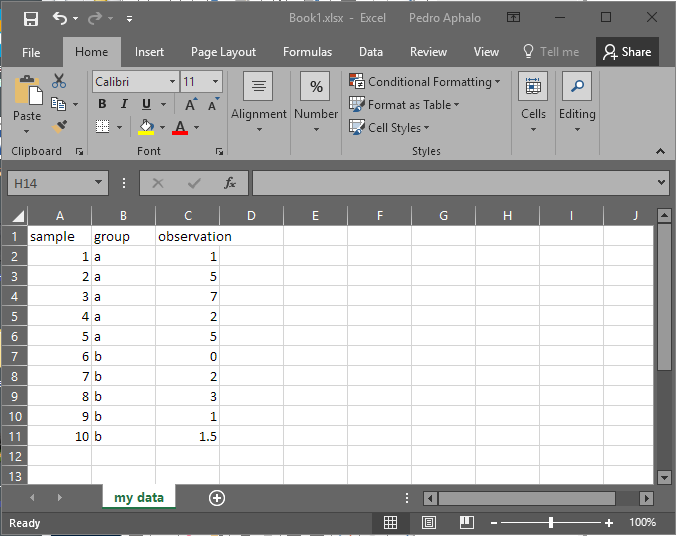
\includegraphics[width=0.75\textwidth]{figures/Book1-xlsx.png}
\end{center}

We first list the sheets contained in the workbook file with \Rfunction{excel\_sheets()}.
\begin{knitrout}\footnotesize
\definecolor{shadecolor}{rgb}{0.969, 0.969, 0.969}\color{fgcolor}\begin{kframe}
\begin{alltt}
\hlstd{sheets} \hlkwb{<-} \hlkwd{excel_sheets}\hlstd{(}\hlstr{"extdata/Book1.xlsx"}\hlstd{)}
\hlstd{sheets}
\end{alltt}
\begin{verbatim}
## [1] "my data"
\end{verbatim}
\end{kframe}
\end{knitrout}

In this case the argument passed to \code{sheet} is redundant, as there is only a single worksheet in the file. It is possible to use either the name of the sheet or a positional index (in this case \code{1} would be equivalent to \code{"my data"}). We use function \Rfunction{read\_excel()} to import the worksheet.
\begin{knitrout}\footnotesize
\definecolor{shadecolor}{rgb}{0.969, 0.969, 0.969}\color{fgcolor}\begin{kframe}
\begin{alltt}
\hlstd{Book1.df} \hlkwb{<-} \hlkwd{read_excel}\hlstd{(}\hlstr{"extdata/Book1.xlsx"}\hlstd{,} \hlkwc{sheet} \hlstd{=} \hlstr{"my data"}\hlstd{)}
\hlstd{Book1.df}
\end{alltt}
\begin{verbatim}
## # A tibble: 10 x 3
##    sample group observation
##     <dbl> <chr>       <dbl>
##  1   1.00 a            1.00
##  2   2.00 a            5.00
##  3   3.00 a            7.00
##  4   4.00 a            2.00
##  5   5.00 a            5.00
##  6   6.00 b            0   
##  7   7.00 b            2.00
##  8   8.00 b            3.00
##  9   9.00 b            1.00
## 10  10.0  b            1.50
\end{verbatim}
\end{kframe}
\end{knitrout}

Of the remaining arguments, \code{skip} is useful when we need to skip the top row of a worksheet.

\subsubsection['xlsx']{\pkgname{xlsx}}

\begin{knitrout}\footnotesize
\definecolor{shadecolor}{rgb}{0.969, 0.969, 0.969}\color{fgcolor}\begin{kframe}
\begin{alltt}
\hlkwd{citation}\hlstd{(}\hlkwc{package} \hlstd{=} \hlstr{"xlsx"}\hlstd{)}
\end{alltt}
\begin{verbatim}
## 
## To cite package 'xlsx' in publications use:
## 
##   Adrian A. Dragulescu (2014). xlsx: Read, write, format Excel
##   2007 and Excel 97/2000/XP/2003 files. R package version 0.5.7.
##   https://CRAN.R-project.org/package=xlsx
## 
## A BibTeX entry for LaTeX users is
## 
##   @Manual{,
##     title = {xlsx: Read, write, format Excel 2007 and Excel 97/2000/XP/2003 files},
##     author = {Adrian A. Dragulescu},
##     year = {2014},
##     note = {R package version 0.5.7},
##     url = {https://CRAN.R-project.org/package=xlsx},
##   }
## 
## ATTENTION: This citation information has been auto-generated from
## the package DESCRIPTION file and may need manual editing, see
## 'help("citation")'.
\end{verbatim}
\end{kframe}
\end{knitrout}

Package \pkgname{xlsx} can be more difficult to install as it uses Java functions to do the actual work. However, it is more comprehensive, with functions both for reading and writing Excel worksheet and workbooks, in different formats. It also allows selecting regions of a worksheet to be imported.

Here we use function \Rfunction{read.xlsx()}, idexing the worksheet by name.

\begin{knitrout}\footnotesize
\definecolor{shadecolor}{rgb}{0.969, 0.969, 0.969}\color{fgcolor}\begin{kframe}
\begin{alltt}
\hlstd{Book1_xlsx.df} \hlkwb{<-} \hlkwd{read.xlsx}\hlstd{(}\hlstr{"extdata/Book1.xlsx"}\hlstd{,} \hlkwc{sheetName} \hlstd{=} \hlstr{"my data"}\hlstd{)}
\hlstd{Book1_xlsx.df}
\end{alltt}
\begin{verbatim}
##    sample group observation
## 1       1     a         1.0
## 2       2     a         5.0
## 3       3     a         7.0
## 4       4     a         2.0
## 5       5     a         5.0
## 6       6     b         0.0
## 7       7     b         2.0
## 8       8     b         3.0
## 9       9     b         1.0
## 10     10     b         1.5
\end{verbatim}
\end{kframe}
\end{knitrout}

As above, but indexing by a numeric index.

\begin{knitrout}\footnotesize
\definecolor{shadecolor}{rgb}{0.969, 0.969, 0.969}\color{fgcolor}\begin{kframe}
\begin{alltt}
\hlstd{Book1_xlsx2.df} \hlkwb{<-} \hlkwd{read.xlsx2}\hlstd{(}\hlstr{"extdata/Book1.xlsx"}\hlstd{,} \hlkwc{sheetIndex} \hlstd{=} \hlnum{1}\hlstd{)}
\hlstd{Book1_xlsx2.df}
\end{alltt}
\begin{verbatim}
##    sample group observation
## 1       1     a           1
## 2       2     a           5
## 3       3     a           7
## 4       4     a           2
## 5       5     a           5
## 6       6     b           0
## 7       7     b           2
## 8       8     b           3
## 9       9     b           1
## 10     10     b         1.5
\end{verbatim}
\end{kframe}
\end{knitrout}

With the three different functions we get a data frame or a tibble, which is compatible with data frames.
\begin{knitrout}\footnotesize
\definecolor{shadecolor}{rgb}{0.969, 0.969, 0.969}\color{fgcolor}\begin{kframe}
\begin{alltt}
\hlkwd{class}\hlstd{(Book1.df)}
\end{alltt}
\begin{verbatim}
## [1] "tbl_df"     "tbl"        "data.frame"
\end{verbatim}
\begin{alltt}
\hlkwd{class}\hlstd{(Book1_xlsx.df)}
\end{alltt}
\begin{verbatim}
## [1] "data.frame"
\end{verbatim}
\begin{alltt}
\hlkwd{class}\hlstd{(Book1_xlsx2.df)}
\end{alltt}
\begin{verbatim}
## [1] "data.frame"
\end{verbatim}
\end{kframe}
\end{knitrout}

However, the columns are imported differently. Both \code{Book1.df} and \code{Book1\_xlsx.df} differ only in that the second column, a character variable, has been converted into a factor or not. This is to be expected as packages in the \pkgname{tidyverse} suite default to preserving character variables as such, while base R functions convert them to factors. The third function, \Rfunction{read.xlsx2()}, did not decode numeric values correctly, and converted everything into factors. This function is reported as being much faster than \Rfunction{read.xlsx()}.
\begin{knitrout}\footnotesize
\definecolor{shadecolor}{rgb}{0.969, 0.969, 0.969}\color{fgcolor}\begin{kframe}
\begin{alltt}
\hlkwd{sapply}\hlstd{(Book1.df, class)}
\end{alltt}
\begin{verbatim}
##      sample       group observation 
##   "numeric" "character"   "numeric"
\end{verbatim}
\begin{alltt}
\hlkwd{sapply}\hlstd{(Book1_xlsx.df, class)}
\end{alltt}
\begin{verbatim}
##      sample       group observation 
##   "numeric"    "factor"   "numeric"
\end{verbatim}
\begin{alltt}
\hlkwd{sapply}\hlstd{(Book1_xlsx2.df, class)}
\end{alltt}
\begin{verbatim}
##      sample       group observation 
##    "factor"    "factor"    "factor"
\end{verbatim}
\end{kframe}
\end{knitrout}

With function \Rfunction{write.xlsx()} we can also write data frames out to Excel worksheets and even append new worksheets to an existing workbook.
\begin{knitrout}\footnotesize
\definecolor{shadecolor}{rgb}{0.969, 0.969, 0.969}\color{fgcolor}\begin{kframe}
\begin{alltt}
\hlkwd{set.seed}\hlstd{(}\hlnum{456321}\hlstd{)}
\hlstd{my.data} \hlkwb{<-} \hlkwd{data.frame}\hlstd{(}\hlkwc{x} \hlstd{=} \hlnum{1}\hlopt{:}\hlnum{10}\hlstd{,} \hlkwc{y} \hlstd{=} \hlnum{1}\hlopt{:}\hlnum{10} \hlopt{+} \hlkwd{rnorm}\hlstd{(}\hlnum{10}\hlstd{))}
\hlkwd{write.xlsx}\hlstd{(my.data,} \hlkwc{file} \hlstd{=} \hlstr{"extdata/my-data.xlsx"}\hlstd{,} \hlkwc{sheetName} \hlstd{=} \hlstr{"first copy"}\hlstd{)}
\hlkwd{write.xlsx}\hlstd{(my.data,} \hlkwc{file} \hlstd{=} \hlstr{"extdata/my-data.xlsx"}\hlstd{,} \hlkwc{sheetName} \hlstd{=} \hlstr{"second copy"}\hlstd{,} \hlkwc{append} \hlstd{=} \hlnum{TRUE}\hlstd{)}
\end{alltt}
\end{kframe}
\end{knitrout}

When opened in Excel we get a workbook, containing two worksheets, named using the arguments we passed through \code{sheetName} in the code chunk above.
\begin{center}
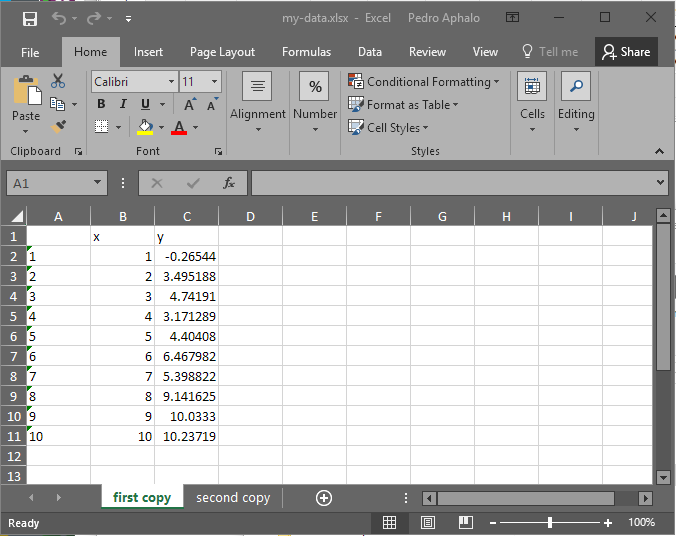
\includegraphics[width=0.75\textwidth]{figures/my-data-xlsx.png}
\end{center}

\begin{playground}
If you have some worksheet files available, import them into R, to get a feel of how the way data is organized in the worksheets affects how easy or difficult it is to read the data from them.
\end{playground}

\subsubsection['xml2']{\pkgname{xml2}}

\begin{knitrout}\footnotesize
\definecolor{shadecolor}{rgb}{0.969, 0.969, 0.969}\color{fgcolor}\begin{kframe}
\begin{alltt}
\hlkwd{citation}\hlstd{(}\hlkwc{package} \hlstd{=} \hlstr{"xml2"}\hlstd{)}
\end{alltt}
\begin{verbatim}
## 
## To cite package 'xml2' in publications use:
## 
##   Hadley Wickham, James Hester and Jeroen Ooms (2017). xml2: Parse
##   XML. R package version 1.1.1.
##   https://CRAN.R-project.org/package=xml2
## 
## A BibTeX entry for LaTeX users is
## 
##   @Manual{,
##     title = {xml2: Parse XML},
##     author = {Hadley Wickham and James Hester and Jeroen Ooms},
##     year = {2017},
##     note = {R package version 1.1.1},
##     url = {https://CRAN.R-project.org/package=xml2},
##   }
\end{verbatim}
\end{kframe}
\end{knitrout}

Several modern data exchange formats are based on the XML standard format which uses schema for flexibility. Package \pkgname{xml2} provides functions for reading and parsing such files, as well as HTML files. This is a vast subject, of which I will only give a brief introduction.

We first read a very simple web page with function \Rfunction{read\_html()}.

\begin{knitrout}\footnotesize
\definecolor{shadecolor}{rgb}{0.969, 0.969, 0.969}\color{fgcolor}\begin{kframe}
\begin{alltt}
\hlstd{web_page} \hlkwb{<-} \hlkwd{read_html}\hlstd{(}\hlstr{"http://r4photobiology.info/R/index.html"}\hlstd{)}
\hlkwd{html_structure}\hlstd{(web_page)}
\end{alltt}
\begin{verbatim}
## <html>
##   <head>
##     <title>
##       {text}
##     <meta [name, content]>
##     <meta [name, content]>
##     <meta [name, content]>
##   <body>
##     {text}
##     <hr>
##     <h1>
##       {text}
##     {text}
##     <hr>
##     <p>
##       {text}
##       <a [href]>
##         {text}
##       {text}
##     {text}
##     <address>
##       {text}
##     {text}
\end{verbatim}
\end{kframe}
\end{knitrout}

And we extract the text from its \code{title} attribute, using functions \Rfunction{xml\_find\_all()} and \Rfunction{xml\_text()}.

\begin{knitrout}\footnotesize
\definecolor{shadecolor}{rgb}{0.969, 0.969, 0.969}\color{fgcolor}\begin{kframe}
\begin{alltt}
\hlkwd{xml_text}\hlstd{(}\hlkwd{xml_find_all}\hlstd{(web_page,} \hlstr{".//title"}\hlstd{))}
\end{alltt}
\begin{verbatim}
## [1] "r4photobiology repository"
\end{verbatim}
\end{kframe}
\end{knitrout}

The functions defined in this package and in package \pkgname{XML} can be used to ``harvest'' data from web pages, but also to read data from files using formats that are defined through XML schemas.

\subsection{Statistical software}\label{sec:files:stat}

There are two different comprehensive packages for importing data saved from other statistical such as SAS, Statistica, SPSS, etc. The long time ``standard'' the \pkgname{foreign} package and the much newer \pkgname{haven}. In the case of files saved with old versions of statistical programs, functions from \pkgname{foreign} tend to be more more robust than those from \pkgname{haven}.

\subsubsection[foreign]{\pkgname{foreign}}

\begin{knitrout}\footnotesize
\definecolor{shadecolor}{rgb}{0.969, 0.969, 0.969}\color{fgcolor}\begin{kframe}
\begin{alltt}
\hlkwd{citation}\hlstd{(}\hlkwc{package} \hlstd{=} \hlstr{"foreign"}\hlstd{)}
\end{alltt}
\begin{verbatim}
## 
## To cite package 'foreign' in publications use:
## 
##   R Core Team (2017). foreign: Read Data Stored by 'Minitab', 'S',
##   'SAS', 'SPSS', 'Stata', 'Systat', 'Weka', 'dBase', .... R
##   package version 0.8-69.
##   https://CRAN.R-project.org/package=foreign
## 
## A BibTeX entry for LaTeX users is
## 
##   @Manual{,
##     title = {foreign: Read Data Stored by 'Minitab', 'S', 'SAS', 'SPSS', 'Stata',
## 'Systat', 'Weka', 'dBase', ...},
##     author = {{R Core Team}},
##     year = {2017},
##     note = {R package version 0.8-69},
##     url = {https://CRAN.R-project.org/package=foreign},
##   }
\end{verbatim}
\end{kframe}
\end{knitrout}

Functions in this package allow to import data from files saved by several foreign statistical analysis programs, including \pgrmname{SAS}, \pgrmname{Stata} and \pgrmname{SPPS} among others, and a function for writing data into files with formats native to these three programs. Documentation is included with R describing them in \emph{R Data Import/Export}. As a simple example we use function \Rfunction{read.spss()} to read a \texttt{.sav} file, saved with a recent version of \pgrmname{SPSS}.

\begin{knitrout}\footnotesize
\definecolor{shadecolor}{rgb}{0.969, 0.969, 0.969}\color{fgcolor}\begin{kframe}
\begin{alltt}
\hlstd{my_spss.df} \hlkwb{<-} \hlkwd{read.spss}\hlstd{(}\hlkwc{file} \hlstd{=} \hlstr{"extdata/my-data.sav"}\hlstd{,} \hlkwc{to.data.frame} \hlstd{=} \hlnum{TRUE}\hlstd{)}
\end{alltt}


{\ttfamily\noindent\itshape\color{messagecolor}{\#\# re-encoding from UTF-8}}\begin{alltt}
\hlkwd{head}\hlstd{(my_spss.df)}
\end{alltt}
\begin{verbatim}
##   block       treat mycotreat water1 pot harvest meas_order spad psi H_mm
## 1     0 Watered, EM         1      1  14       1         NA   NA  NA   67
## 2     0 Watered, EM         1      1  52       1         NA   NA  NA   44
## 3     0 Watered, EM         1      1 111       1         NA   NA  NA   65
## 4     0 Watered, EM         1      1 127       1         NA   NA  NA   78
## 5     0 Watered, EM         1      1 230       1         NA   NA  NA   71
## 6     0 Watered, EM         1      1 258       1         NA   NA  NA  100
##    d_mm pot_plant_g plant_g tag_g pot_g leaf_area harvest_date stem_g
## 1 2.115          NA      NA    NA    NA    35.883  13653705600 0.0372
## 2 1.285          NA      NA    NA    NA    16.938  13653705600 0.0139
## 3 1.685          NA      NA    NA    NA    38.056  13653705600 0.0279
## 4 1.870          NA      NA    NA    NA    38.469  13653705600 0.0389
## 5 1.900          NA      NA    NA    NA    39.917  13653705600 0.0446
## 6 1.810          NA      NA    NA    NA    45.968  13653705600 0.0513
##   leaves_g green_leaves save_order waterprcnt height_1 height_2 height_3
## 1   0.1685       0.0542          1         NA       23       34       55
## 2   0.0626       0.0443          2         NA       10       21       37
## 3   0.1522       0.0511          3         NA       12       27       48
## 4   0.1462       0.0500          4         NA       30       40       64
## 5   0.1696       0.0677          5         NA       28       37       60
## 6   0.1959       0.0741          6         NA       42       60       84
##   height_4 diam_1 height_5 diam_2
## 1       NA     NA       NA     NA
## 2       NA     NA       NA     NA
## 3       NA     NA       NA     NA
## 4       NA     NA       NA     NA
## 5       NA     NA       NA     NA
## 6       NA     NA       NA     NA
\end{verbatim}
\end{kframe}
\end{knitrout}

Dates were not converted into R's datetime objects, but instead into numbers.

A second example, this time with a simple \code{.sav} file saved 15 years ago.

\begin{knitrout}\footnotesize
\definecolor{shadecolor}{rgb}{0.969, 0.969, 0.969}\color{fgcolor}\begin{kframe}
\begin{alltt}
\hlstd{thiamin.df} \hlkwb{<-} \hlkwd{read.spss}\hlstd{(}\hlkwc{file} \hlstd{=} \hlstr{"extdata/thiamin.sav"}\hlstd{,} \hlkwc{to.data.frame} \hlstd{=} \hlnum{TRUE}\hlstd{)}
\hlkwd{head}\hlstd{(thiamin.df)}
\end{alltt}
\begin{verbatim}
##   THIAMIN CEREAL
## 1     5.2  wheat
## 2     4.5  wheat
## 3     6.0  wheat
## 4     6.1  wheat
## 5     6.7  wheat
## 6     5.8  wheat
\end{verbatim}
\end{kframe}
\end{knitrout}

Another example, for a Systat file saved on an PC more than 20 years ago, and rea.

\begin{knitrout}\footnotesize
\definecolor{shadecolor}{rgb}{0.969, 0.969, 0.969}\color{fgcolor}\begin{kframe}
\begin{alltt}
\hlstd{my_systat.df} \hlkwb{<-} \hlkwd{read.systat}\hlstd{(}\hlkwc{file} \hlstd{=} \hlstr{"extdata/BIRCH1.SYS"}\hlstd{)}
\hlstd{my_systat.df}
\end{alltt}
\begin{verbatim}
##     CONT DENS BLOCK SEEDL VITAL BASE ANGLE HEIGHT DIAM
## 1      1    1     1     2    44    2     0      1   53
## 2      1    1     1     2    41    2     1      2   70
## 3      1    1     1     2    21    2     0      1   65
## 4      1    1     1     2    15    3     0      1   79
## 5      1    1     1     2    37    3     0      1   71
## 6      1    1     1     2    29    2     1      1   43
## 7      1    1     1     1    30    0    NA     NA   NA
## 8      1    1     1     1    28    0    NA     NA   NA
## 9      1    1     1     1    37    3     2      1   74
## 10     1    1     1     1    26    3     1      3   71
## 11     1    1     1     1    27    3     0      1   64
## 12     1    1     1     1    45    0    NA     NA   NA
## 13     1    1     4     2    41    3     2      1   76
## 14     1    1     4     2    32    1     1      3   35
## 15     1    1     4     2    19    3     1      2   79
## 16     1    1     4     2    20    2     0      2   70
## 17     1    1     4     2     3    2     2      3   75
## 18     1    1     4     2     5    0    NA     NA   NA
## 19     1    1     4     1    28    2     1      2   80
## 20     1    1     4     1    41    2     1      3   73
## 21     1    1     4     1    36    1     0      1   21
## 22     1    1     4     1    43    2     0      2   51
## 23     1    1     4     1    22    2     1      2   66
## 24     1    1     4     1    31    3     1      2   84
## 25     1    1     3     2    30    2     0      1   49
## 26     1    1     3     2     4    2     2      1   42
## 27     1    1     3     2    35    3     2      2   90
## 28     1    1     3     2    43    2     1      2   60
## 29     1    1     3     2    12    3     0      1   65
## 30     1    1     3     1    35    2     0      1   61
## 31     1    1     3     1    36    2     0      2   65
## 32     1    1     3     1     7    3     2      1   83
## 33     1    1     3     1     9    2     3      2   68
## 34     1    1     3     1    20    2     1      1   65
## 35     1    1     3     1    11    2     1      1   53
## 36     1    1     3     1    14    2     0      1   60
## 37     1    1     1     3    30    2     0      1   59
## 38     1    1     1     3    15    2     2      2   65
## 39     1    1     1     3    14    2     2      2   77
## 40     1    1     1     3    32    3     0      1   72
## 41     1    1     1     3    38    3     2      2   78
## 42     1    1     1     3    13    2     1      1   56
## 43     1    1     4     2    41    3     2      1   77
## 44     1    1     4     2    32    1     1      2   34
## 45     1    1     4     2    19    3     1      2   80
## 46     1    1     4     2    20    3     0      2   70
## 47     1    1     4     2     3    2     1      2   75
## 48     1    1     4     1    28    3     1      2   80
## 49     1    1     4     1    41    2     1      2   73
## 50     1    1     4     1    36    1     0      1   21
## 51     1    1     4     1    43    2     0      1   51
## 52     1    1     4     1    22    2     1      2   66
## 53     1    1     4     1    31    3     1      2   84
## 54     1    1     3     2    30    2     0      1   49
## 55     1    1     3     2     4    2     2      1   42
## 56     1    1     3     2    35    3     2      2   89
## 57     1    1     3     2    43    2     1      2   60
## 58     1    1     3     2    12    3     0      1   65
## 59     1    1     3     1    35    2     0      1   60
## 60     1    1     3     1    36    2     0      1   66
## 61     1    1     3     1     7    3     2      1   83
## 62     1    1     3     1     9    2     3      2   68
## 63     1    1     3     1    20    2     1      1   65
## 64     1    1     3     1    11    2     1      1   54
## 65     1    1     3     1    14    2     0      1   60
## 66     1    1     2     3    29    2     1      1   47
## 67     1    1     2     3    27    2     0      1   67
## 68     1    1     2     3    45    3     1      1   74
## 69     1    1     2     3    40    0    NA     NA   NA
## 70     1    1     2     3    33    1     1      1   47
## 71     1    1     2     3    19    2     1      1   57
## 72     1    1     2     2    18    3     0      1   74
## 73     1    1     2     1     2    2     0      3   71
## 74     1    1     2     2    33    3     1      1   80
## 75     1    1     2     1    16    0    NA     NA   NA
## 76     1    1     2     1    44    0    NA     NA   NA
## 77     1    1     2     1    34    2     1      1   54
## 78     1    1     2     2    32    3     0      1   77
## 79     1    1     2     2    21    3     1      1   74
## 80     1    1     2     1    13    3     1      1   69
## 81     1    1     2     1     3    3     1      1   72
## 82     1    1     2     2     7    0    NA     NA   NA
## 83     1    1     2     2    39    2     1      1   54
## 84     1    2     1     4     5    2     1      2   67
## 85     1    2     1     4    14    2     1      2   46
## 86     1    2     1     4    17    2     1      1   64
## 87     1    2     1     3     7    3     0      1  100
## 88     1    2     1     3     9    3     2      2   69
## 89     1    2     1     3    13    3     1      1   74
## 90     1    2     1     3    12    3     0      1   71
## 91     1    2     3     1     1    0    NA     NA   NA
## 92     1    2     3     1     6    2     2      1   35
## 93     1    2     3     1    15    2     0      1   38
## 94     1    2     3     4    10    2     1      1   65
## 95     1    2     3     4     1    2     0      2   72
## 96     1    2     3     3    23    2     2      2   66
## 97     1    2     3     3    20    1     0      1   17
## 98     1    2     3     3    12    3     2      1   71
## 99     1    2     3     3    21    2     1      1   43
## 100    1    2     3     2     4    2     0      1   44
## 101    1    2     3     2    14    1     0      1   20
## 102    1    2     3     2    18    2     1      2   57
## 103    1    2     3     5    18    2     0      2   54
## 104    1    2     3     5     9    2     3      2   55
## 105    1    2     3     5    16    2     1      1   57
## 106    1    2     3     5    17    3     0      1   73
## 107    1    2     3     4    16    2     1      1   30
## 108    1    2     4     1    14    3     1      1   84
## 109    1    2     4     1    12    3     0      1   75
## 110    1    2     4     3    17    2     0      1   65
## 111    1    2     4     3    15    3     0      1   81
## 112    1    2     4     2     5    2     1      1   62
## 113    1    2     4     2     7    3     0      1   84
## 114    1    2     4     2     6    2     0      1   66
## 115    1    2     4     1    17    3     1      1   73
## 116    1    2     4     1    10    3     0      1   88
## 117    1    2     4     3     5    2     0      1   61
## 118    1    2     2     3    18    3     0      1   87
## 119    1    2     2     3    21    3     0      1   74
## 120    1    2     2     1     3    2     2      3   60
## 121    1    2     2     1    13    2     0      2   63
## 122    1    2     2     1    12    3     1      2   69
## 123    1    2     2     3     2    3     0      1   81
## 124    1    2     4     3     5    2     0      1   61
## 125    1    2     2     3    18    3     0      1   87
## 126    1    2     2     3    21    3     0      1   74
## 127    1    2     2     1     3    2     2      2   60
## 128    1    2     2     1    13    2     0      2   63
## 129    1    2     2     1    12    3     1      1   70
## 130    1    2     2     3     2    3     0      1   81
## 131    1    2     1     1     5    3     1      1   72
## 132    1    2     1     1    21    2     0      1   48
## 133    1    2     1     1    12    2     0      1   44
## 134    1    2     1     1    10    2     1      2   50
## 135    1    2     4     4    22    3     0      1   80
## 136    1    2     4     4     5    2     1      1   53
## 137    1    2     4     4     2    3     0      1   79
## 138    1    2     4     5    22    3     1      2   77
## 139    1    2     4     5    20    2     1      1   52
## 140    1    2     4     5    16    3     1      1   77
## 141    1    2     2     2     4    3     0      1   75
## 142    1    2     2     2     7    3     1      1   83
## 143    1    2     2     2    13    2     1      1   48
## 144    1    2     2     4    21    2     1      1   55
## 145    1    2     2     4    20    2     1      1   55
## 146    1    2     2     4    16    3     0      1   81
## 147    1    2     2     4    11    3     1      2   76
## 148    1    2     1     2     4    2     2      1   64
## 149    1    2     1     2     6    3     1      1   87
## 150    1    2     1     2     5    2     2      1   60
## 151    1    3     3     1     4    2     0      2   63
## 152    1    3     3     2     4    2     0      1   70
## 153    1    3     3     2     5    3     1      1   82
## 154    1    3     3     3     4    0     0      1   95
## 155    1    3     3     6     3    2     0      1   51
## 156    1    3     3     6     6    2     0      2   49
## 157    1    3     3     7    10    2     0      2   66
## 158    1    3     3     8     7    3     1      2   74
## 159    1    3     3     1     2    2     0      1   54
## 160    1    3     3     6     6    2     0      1   49
## 161    1    3     3     6     3    2     0      1   51
## 162    1    3     3     7    10    2     1      1   66
## 163    1    3     3     8     7    3     0      2   74
## 164    1    3     3     1     2    2     0      1   54
## 165    1    3     1     8     2    2     0      2   68
## 166    1    3     4     3    10    3     1      2   80
## 167    1    3     4     2    10    3     1      1   87
## 168    1    3     4     9     8    1     0      1   36
## 169    1    3     4     9     3    1     3      2   56
## 170    1    3     3     5    12    3     1      2   82
## 171    1    3     1     8     8    2     0      1   70
## 172    1    3     4     1    11    2     0      1   51
## 173    1    3     4     6     2    2     1      1   52
## 174    1    3     4     8     9    2     0      1   67
## 175    1    3     3     5    10    2     0      1   42
## 176    1    3     1     7    10    3     1      1   78
## 177    1    3     4     1     8    2     0      1   61
## 178    1    3     4     6    10    2     1      1   44
## 179    1    3     4     8     5    3     1      1   91
## 180    1    3     3     4     6    3     1      1   91
## 181    1    3     4     7     1    3     0      1   80
## 182    1    3     4     5     2    2     0      1   51
## 183    1    3     4     4    12    2     0      1   55
## 184    1    3     1     7     6    2     1      1   68
## 185    1    3     4     4     4    2     0      1   68
## 186    1    3     4     5    10    3     0      1   78
## 187    1    3     4     7     8    2     0      1   27
## 188    1    3     3    10    13    2     1      2   75
## 189    1    3     3    10    10    2     1      2   61
## 190    1    3     3     9     8    2     0      1   60
## 191    1    3     3     9     2    3     0      1   85
## 192    1    3     1     5     3    3     1      1   81
## 193    1    3     2     5     1    3     1      2   77
## 194    1    3     1     1     3    3     1      1   86
## 195    1    3     1     2     3    3     0      2   75
## 196    1    3     1     5     6    2     0      1   63
## 197    1    3     2     5     9    3     1      1   74
## 198    1    3     1     1     2    2     1      1   62
## 199    1    3     1     2    12    2     0      1   46
## 200    1    3     1     6    12    2     0      1   46
## 201    1    3     1     3     8    2     3      1   63
## 202    1    3     2     6     2    3     2      1   75
## 203    1    3     2     8     9    2     1      1   39
## 204    1    3     2     1     5    2     1      2   58
## 205    1    3     2     3    12    2     1      1   61
## 206    1    3     1     4     9    2     1      1   52
## 207    1    3     2     4    11    2     1      1   54
## 208    1    3     2     1     9    3     1      1   76
## 209    1    3     2     8    12    2     0      1   44
## 210    1    3     2     6    13    3     1      1   71
## 211    1    3     2     2     3    2     1      2   49
## 212    1    3     2     2    10    3     0      1   67
## 213    1    3     2     7     6    2     1      1   63
## 214    1    3     2     7     2    3     0      1   75
## 215    1    3     1     4     3    2     1      1   57
## 216    2    1     1     4    12    2     1      3   64
## 217    2    1     1     4    13    0    NA     NA   NA
## 218    2    1     1     1    17    3     1      1   92
## 219    2    1     1     3    16    3     2      1  106
## 220    2    1     1     3     5    3     1      1   93
## 221    2    1     1     3    13    3     0      1  101
## 222    2    1     1     1    19    3     0      1   72
## 223    2    1     1     4     1    3     0      2   90
## 224    2    1     1     2     7    3     0      2   93
## 225    2    1     1     2    19    3     0      1   90
## 226    2    1     1     2    20    3     0      1   87
## 227    2    1     1     2    11    3     0      2   96
## 228    2    1     1     1    15    3     1      2   90
## 229    2    1     1     3    15    3     1      1   96
## 230    2    1     1     1    27    2     2      2   46
## 231    2    1     2     3    18    2     0      1   71
## 232    2    1     3     2     6    3     0      1  101
## 233    2    1     2     3     9    3     0      2   76
## 234    2    1     3     2    28    3     1      1   82
## 235    2    1     3     4    19    3     0      1   75
## 236    2    1     2     3    26    2     1      1   60
## 237    2    1     3     2    15    3     1      1   89
## 238    2    1     3     1     3    3     1      1   92
## 239    2    1     3     4    25    2     0      2   67
## 240    2    1     2     3    27    3     0      1   87
## 241    2    1     3     2    25    2     1      1   66
## 242    2    1     3     1    22    2     2      1   61
## 243    2    1     3     4    11    3     1      1  100
## 244    2    1     3     1    10    3     0      1   86
## 245    2    1     3     1    15    2     0      1   61
## 246    2    1     3     4    17    3     0      1   92
## 247    2    1     4     1    17    3     1      1   94
## 248    2    1     4     1    22    2     1      1   70
## 249    2    1     3     3    22    3     1      1   85
## 250    2    1     3     3    21    3     0      2   85
## 251    2    1     3     3     4    0    NA     NA   NA
## 252    2    1     3     3    12    0    NA     NA   NA
## 253    2    1     4     1     3    3     1      1   80
## 254    2    1     4     1    21    3     0      1   74
## 255    2    1     4     2     3    3     1      1   59
## 256    2    1     4     2    19    3     1      2   82
## 257    2    1     4     2    24    2     0      2   82
## 258    2    1     4     2    11    2     1      2   70
## 259    2    1     4     3    28    1     3      1   28
## 260    2    1     4     3     7    2     1      1   69
## 261    2    1     4     3    11    2     1      3   82
## 262    2    1     4     3    13    3     0      1   89
## 263    2    1     2     2    24    2     0      1   76
## 264    2    1     2     2     3    3     1      1   78
## 265    2    1     2     2    12    3     1      1   88
## 266    2    1     2     1     4    3     1      2   80
## 267    2    1     2     1    27    3     1      1   86
## 268    2    1     2     1    26    3     0      1   81
## 269    2    1     2     1    11    3     1      1   88
## 270    2    1     2     2     8    2     1      1   34
## 271    2    1     2     4    12    3     1      1   83
## 272    2    1     2     4     5    3     1      1   86
## 273    2    1     2     4    15    3     1      1   88
## 274    2    1     2     4    24    2     1      1   54
## 275    2    2     2     8     6    2     0      1   70
## 276    2    2     4     1    12    3     0      1   78
## 277    2    2     3     5     1    3     1      1   99
## 278    2    2     3     2    10    3     1      1   90
## 279    2    2     3     1     4    0    NA     NA   NA
## 280    2    2     3     5    10    3     1      1   80
## 281    2    2     2     8    12    3     0      1   91
## 282    2    2     3     3    13    0    NA     NA   NA
## 283    2    2     3     4     2    3     0      1   88
## 284    2    2     4     7     8    3     0      2   86
## 285    2    2     4     7     5    3     2      1   79
## 286    2    2     3     4     3    3     0      2   83
## 287    2    2     3     6     6    3     1      1   99
## 288    2    2     4     1    10    2     0      2   68
## 289    2    2     3     6    13    3     0      1   86
## 290    2    2     1     3     1    2     1      2   82
## 291    2    2     1     6    12    3     1      1   73
## 292    2    2     1     7     6    3     2      2   82
## 293    2    2     1     7     3    3     0      2   86
## 294    2    2     1     1     7    3     0      1   92
## 295    2    2     1     4     9    3     0      1   78
## 296    2    2     1     5     4    2     2      1   67
## 297    2    2     1     8     1    3     0      1   87
## 298    2    2     3     1     8    1     2      2   52
## 299    2    2     1     1    14    3     0      2   90
## 300    2    2     1     4    12    3     0      1   86
## 301    2    2     1     5     9    3     1      3   97
## 302    2    2     1     8     9    3     0      1   85
## 303    2    2     3     1     6    3     0      1  116
## 304    2    2     1     2     6    2     2      3   70
## 305    2    2     1     2    10    1     2      1   39
## 306    2    2     1     3     6    3     2      1   91
## 307    2    2     1     6     2    3     1      2   83
## 308    2    2     4     2    10    2     1      3   62
## 309    2    2     4     2     2    2     1      2   72
## 310    2    2     2     3     3    2     0      4   59
## 311    2    2     4     6     7    3     1      1   76
## 312    2    2     2     3    10    3     0      1   82
## 313    2    2     4     6    12    3     0      1   69
## 314    2    2     4     8    13    3     1      1   92
## 315    2    2     2     4    14    3     1      1   85
## 316    2    2     2     7    11    3     1      2   95
## 317    2    2     4     3     6    3     0      1   86
## 318    2    2     2     7    14    3     0      3   97
## 319    2    2     4     5    12    3     1      1  106
## 320    2    2     4     8     6    3     1      1  103
## 321    2    2     2     4     9    3     0      2   97
## 322    2    2     4     3     3    3     1      1   95
## 323    2    2     4     5     2    3     0      1   80
## 324    2    2     4     4    11    3     1      1   85
## 325    2    2     4     4     9    3     1      1   86
## 326    2    2     2     2     6    3     0      1   97
## 327    2    2     2     2     7    2     0      1   69
## 328    2    2     2     1     4    2     0      1   76
## 329    2    2     2     1     6    3     0      1   79
## 330    2    2     2     5     3    3     1      1   94
## 331    2    2     2     5    10    3     1      2   91
## 332    2    2     2     6    10    3     0      1   83
## 333    2    2     2     6     4    3     0      1   94
## 334    2    3     3     1     6    3     0      2   96
## 335    2    3     3     6     7    3     0      1   73
## 336    2    3     2     4     5    3     0      1   78
## 337    2    3     3     7     2    3     0      1   86
## 338    2    3     2     9     3    2     0      1   52
## 339    2    3     3    11     4    3     0      1   92
## 340    2    3     3     8     3    3     0      1   81
## 341    2    3     3    13     7    3     1      1  102
## 342    2    3     3    12     6    3     0      1  113
## 343    2    3     3     3     3    3     0      1  114
## 344    2    3     1     3     3    2     1      1   51
## 345    2    3     1    12     6    3     1      1  106
## 346    2    3     1     2     8    3     0      1   99
## 347    2    3     1     8     6    3     0      1   95
## 348    2    3     1     1     5    0    NA     NA   NA
## 349    2    3     1     7     3    3     0      1   71
## 350    2    3     1     4     4    3     1      1   81
## 351    2    3     1    11     2    3     0      1   75
## 352    2    3     3     2     4    3     1      1   67
## 353    2    3     3     2     3    0    NA     NA   NA
## 354    2    3     1    15     1    3     0      2   88
## 355    2    3     2     3     1    3     0      1   98
## 356    2    3     2     1     2    3     1      1   84
## 357    2    3     2     2     7    3     0      1   82
## 358    2    3     2     8     7    2     0      1   43
## 359    2    3     2     7     3    3     0      1   84
## 360    2    3     2     6     2    3     0      1   62
## 361    2    3     2    13     5    2     0      1   34
## 362    2    3     2    11     4    3     1      1   81
## 363    2    3     1    13     1    3     0      2   97
## 364    2    3     4     8     7    3     0      1   83
## 365    2    3     4     7     3    3     0      2   79
## 366    2    3     4     3     4    3     0      1   84
## 367    2    3     4     9     7    2     0      1   56
## 368    2    3     4     4     7    2     0      1   52
## 369    2    3     4     2     6    2     0      1   63
## 370    2    3     1    14     4    3     1      2  115
## 371    2    3     4     1     4    1     0      3   79
## 372    2    3     2    10     2    3     1      1   89
## 373    2    3     4    10     7    2     0      1   63
## 374    2    3     2    15     7    3     1      1   88
## 375    2    3     4    15     5    2     1      1   59
## 376    2    3     2     5     5    2     1      2   70
## 377    2    3     2    14     6    3     0      1   84
## 378    2    3     4     5     5    3     0      1   79
## 379    2    3     4     6     6    3     0      1   88
## 380    2    3     4    14     5    3     0      1   98
## 381    2    3     4    13     7    3     0      1   77
## 382    2    3     3     4     2    2     0      1   67
## 383    2    3     3     5     3    2     0      1   58
## 384    2    3     4    11     4    2     0      1   72
## 385    2    3     4    12     3    3     0      1  103
## 386    2    3     3    10     6    3     0      1   71
## 387    2    3     3     9     3    3     0      1  112
## 388    2    3     3    15     6    3     1      1   73
## 389    2    3     3    14     7    3     1      1   97
## 390    2    3     1     5     1    3     1      1   88
## 391    2    3     1     6     2    3     1      1   93
## 392    2    3     2    12     4    3     0      1   89
## 393    2    3     1    10     4    2     1      1   67
## 394    2    3     1     9     4    3     0      1   84
\end{verbatim}
\end{kframe}
\end{knitrout}

The functions in \pkgname{foreign} can return data frames, but not always this is the default.

\subsubsection[haven]{\pkgname{haven}}

\begin{knitrout}\footnotesize
\definecolor{shadecolor}{rgb}{0.969, 0.969, 0.969}\color{fgcolor}\begin{kframe}
\begin{alltt}
\hlkwd{citation}\hlstd{(}\hlkwc{package} \hlstd{=} \hlstr{"haven"}\hlstd{)}
\end{alltt}
\begin{verbatim}
## 
## To cite package 'haven' in publications use:
## 
##   Hadley Wickham and Evan Miller (2017). haven: Import and Export
##   'SPSS', 'Stata' and 'SAS' Files. R package version 1.1.0.
##   https://CRAN.R-project.org/package=haven
## 
## A BibTeX entry for LaTeX users is
## 
##   @Manual{,
##     title = {haven: Import and Export 'SPSS', 'Stata' and 'SAS' Files},
##     author = {Hadley Wickham and Evan Miller},
##     year = {2017},
##     note = {R package version 1.1.0},
##     url = {https://CRAN.R-project.org/package=haven},
##   }
\end{verbatim}
\end{kframe}
\end{knitrout}

The recently released package \pkgname{haven} is less ambitious in scope, providing read and write functions for only three file formats: \pgrmname{SAS}, \pgrmname{Stata} and \pgrmname{SPSS}. On the other hand \pkgname{haven} provides flexible ways to convert the different labelled values that cannot be directly mapped to normal R modes. They also decode dates and times according to the idiosyncrasies of each of these file formats. The returned \Rclass{tibble} objects in cases when the imported file contained labelled values needs some further work from the user before obtaining `normal' data-frame-compatible \Rclass{tibble} objects.

We here use function \Rfunction{read\_sav()} to import here a \code{.sav} file saved by a recent version of \pgrmname{SPSS}.

\begin{knitrout}\footnotesize
\definecolor{shadecolor}{rgb}{0.969, 0.969, 0.969}\color{fgcolor}\begin{kframe}
\begin{alltt}
\hlstd{my_spss.tb} \hlkwb{<-} \hlkwd{read_sav}\hlstd{(}\hlkwc{file} \hlstd{=} \hlstr{"extdata/my-data.sav"}\hlstd{)}
\hlstd{my_spss.tb}
\end{alltt}
\begin{verbatim}
## # A tibble: 372 x 29
##    block treat myco~ wate~   pot harv~ meas~  spad   psi  H_mm  d_mm pot_~
##    <dbl> <dbl> <dbl> <dbl> <dbl> <dbl> <dbl> <dbl> <dbl> <dbl> <dbl> <dbl>
##  1     0 1      1.00  1.00  14.0  1.00    NA    NA    NA  67.0  2.12    NA
##  2     0 1      1.00  1.00  52.0  1.00    NA    NA    NA  44.0  1.28    NA
##  3     0 1      1.00  1.00 111    1.00    NA    NA    NA  65.0  1.68    NA
##  4     0 1      1.00  1.00 127    1.00    NA    NA    NA  78.0  1.87    NA
##  5     0 1      1.00  1.00 230    1.00    NA    NA    NA  71.0  1.90    NA
##  6     0 1      1.00  1.00 258    1.00    NA    NA    NA 100    1.81    NA
##  7     0 1      1.00  1.00 363    1.00    NA    NA    NA  85.0  1.76    NA
##  8     0 1      1.00  1.00 400    1.00    NA    NA    NA  59.0  1.68    NA
##  9     0 1      1.00  1.00 424    1.00    NA    NA    NA  77.0  1.56    NA
## 10     0 1      1.00  1.00 443    1.00    NA    NA    NA  68.0  1.68    NA
## # ... with 362 more rows, and 17 more variables: plant_g <dbl>, tag_g
## #   <dbl>, pot_g <dbl>, leaf_area <dbl>, harvest_date <date>, stem_g
## #   <dbl>, leaves_g <dbl>, green_leaves <dbl>, save_order <dbl>,
## #   waterprcnt <dbl>, height_1 <dbl>, height_2 <dbl>, height_3 <dbl>,
## #   height_4 <dbl>, diam_1 <dbl>, height_5 <dbl>, diam_2 <dbl>
\end{verbatim}
\begin{alltt}
\hlkwd{head}\hlstd{(my_spss.tb}\hlopt{$}\hlstd{harvest_date)}
\end{alltt}
\begin{verbatim}
## [1] "2015-06-15" "2015-06-15" "2015-06-15" "2015-06-15" "2015-06-15"
## [6] "2015-06-15"
\end{verbatim}
\end{kframe}
\end{knitrout}

In this case the dates are correctly decoded.

And an \pgrmname{SPSS}'s \code{.sav} file saved 15 years ago.

\begin{knitrout}\footnotesize
\definecolor{shadecolor}{rgb}{0.969, 0.969, 0.969}\color{fgcolor}\begin{kframe}
\begin{alltt}
\hlstd{thiamin.tb} \hlkwb{<-} \hlkwd{read_sav}\hlstd{(}\hlkwc{file} \hlstd{=} \hlstr{"extdata/thiamin.sav"}\hlstd{)}
\hlstd{thiamin.tb}
\end{alltt}
\begin{verbatim}
## # A tibble: 24 x 2
##    THIAMIN CEREAL   
##      <dbl> <dbl+lbl>
##  1    5.20 1        
##  2    4.50 1        
##  3    6.00 1        
##  4    6.10 1        
##  5    6.70 1        
##  6    5.80 1        
##  7    6.50 2        
##  8    8.00 2        
##  9    6.10 2        
## 10    7.50 2        
## # ... with 14 more rows
\end{verbatim}
\begin{alltt}
\hlstd{thiamin.tb} \hlkwb{<-} \hlkwd{as_factor}\hlstd{(thiamin.tb)}
\hlstd{thiamin.tb}
\end{alltt}
\begin{verbatim}
## # A tibble: 24 x 2
##    THIAMIN CEREAL
##      <dbl> <fctr>
##  1    5.20 wheat 
##  2    4.50 wheat 
##  3    6.00 wheat 
##  4    6.10 wheat 
##  5    6.70 wheat 
##  6    5.80 wheat 
##  7    6.50 barley
##  8    8.00 barley
##  9    6.10 barley
## 10    7.50 barley
## # ... with 14 more rows
\end{verbatim}
\end{kframe}
\end{knitrout}

\begin{playground}
Compare the values returned by different \code{read} functions when applied to the same file on disk. Use \Rfunction{names()}, \Rfunction{str()} and \Rfunction{class()} as tools in your exploration. If you are brave, also use \Rfunction{attributes()}, \Rfunction{mode()}, \Rfunction{dim()}, \Rfunction{dimnames()}, \Rfunction{nrow()} and \Rfunction{ncol()}.
\end{playground}

\begin{playground}
If you use or have used in the past other statistical software or a general purpose language like \langname{Python}, look up some files, and import them into R.
\end{playground}

\subsection{NetCDF files}

In some fields including geophysics and meteorology NetCDF is a very common format for the exchange of data. It is also used in other contexts in which data is referenced to an array of locations, like with data read from Affymetrix micro arrays used to study gene expression. The NetCDF format allows the storage of metadata together with the data itself in a well organized and standardized format, which is ideal for exchange of moderately large data sets.

Officially described as
\begin{quote}
NetCDF is a set of software libraries and self-describing, machine-independent data formats that support the creation, access, and sharing of array-oriented scientific data.
\end{quote}

As sometimes NetCDF files are large, it is good that it is possible to selectively read the data from individual variables with functions in packages \pkgname{ncdf4} or \pkgname{RNetCDF}. On the other hand, this implies that contrary to other data file reading operations, reading a NetCDF file is done in two or more steps.

\subsubsection[ncdf4]{\pkgname{ncdf4}}

\begin{knitrout}\footnotesize
\definecolor{shadecolor}{rgb}{0.969, 0.969, 0.969}\color{fgcolor}\begin{kframe}
\begin{alltt}
\hlkwd{citation}\hlstd{(}\hlkwc{package} \hlstd{=} \hlstr{"ncdf4"}\hlstd{)}
\end{alltt}
\begin{verbatim}
## 
## To cite package 'ncdf4' in publications use:
## 
##   David Pierce (2017). ncdf4: Interface to Unidata netCDF (Version
##   4 or Earlier) Format Data Files. R package version 1.16.
##   https://CRAN.R-project.org/package=ncdf4
## 
## A BibTeX entry for LaTeX users is
## 
##   @Manual{,
##     title = {ncdf4: Interface to Unidata netCDF (Version 4 or Earlier) Format Data
## Files},
##     author = {David Pierce},
##     year = {2017},
##     note = {R package version 1.16},
##     url = {https://CRAN.R-project.org/package=ncdf4},
##   }
## 
## ATTENTION: This citation information has been auto-generated from
## the package DESCRIPTION file and may need manual editing, see
## 'help("citation")'.
\end{verbatim}
\end{kframe}
\end{knitrout}

We first need to read an index into the file contents, and in additional steps we read a subset of the data. With \Rfunction{print()} we can find out the names and characteristics of the variables and attributes. In this example we use long term averages for potential evapotranspiration (PET).

We first open a connection to the file with function \Rfunction{nc\_open()}.

\begin{knitrout}\footnotesize
\definecolor{shadecolor}{rgb}{0.969, 0.969, 0.969}\color{fgcolor}\begin{kframe}
\begin{alltt}
\hlstd{meteo_data.nc} \hlkwb{<-} \hlkwd{nc_open}\hlstd{(}\hlstr{"extdata/pevpr.sfc.mon.ltm.nc"}\hlstd{)}
\hlcom{# very long output}
\hlcom{# print(meteo_data.nc)}
\end{alltt}
\end{kframe}
\end{knitrout}

\begin{playground}
Uncomment the \Rfunction{print()} statement above and study the metadata available for the data set as a whole, and for each variable.
\end{playground}
The dimensions of the array data are described with metadata, mapping indexes to in our examples a grid of latitudes and longitudes and a time vector as a third dimension. The dates are returned as character strings. We get here the variables one at a time with function \Rfunction{ncvar\_get()}.

\begin{knitrout}\footnotesize
\definecolor{shadecolor}{rgb}{0.969, 0.969, 0.969}\color{fgcolor}\begin{kframe}
\begin{alltt}
\hlstd{time.vec} \hlkwb{<-} \hlkwd{ncvar_get}\hlstd{(meteo_data.nc,} \hlstr{"time"}\hlstd{)}
\hlkwd{head}\hlstd{(time.vec)}
\end{alltt}
\begin{verbatim}
## [1] -657073 -657042 -657014 -656983 -656953 -656922
\end{verbatim}
\begin{alltt}
\hlstd{longitude} \hlkwb{<-}  \hlkwd{ncvar_get}\hlstd{(meteo_data.nc,} \hlstr{"lon"}\hlstd{)}
\hlkwd{head}\hlstd{(longitude)}
\end{alltt}
\begin{verbatim}
## [1] 0.000 1.875 3.750 5.625 7.500 9.375
\end{verbatim}
\begin{alltt}
\hlstd{latitude} \hlkwb{<-} \hlkwd{ncvar_get}\hlstd{(meteo_data.nc,} \hlstr{"lat"}\hlstd{)}
\hlkwd{head}\hlstd{(latitude)}
\end{alltt}
\begin{verbatim}
## [1] 88.5420 86.6531 84.7532 82.8508 80.9473 79.0435
\end{verbatim}
\end{kframe}
\end{knitrout}

The \code{time} vector is rather odd, as it contains only month data as these are long-term averages. From the metadata we can infer that they correspond to the months of the year, and we directly generate these, instead of attempting a conversion.

We construct a \Rclass{tibble} object with PET values for one grid point, we can take advantage of \emph{recycling} or short vectors.

\begin{knitrout}\footnotesize
\definecolor{shadecolor}{rgb}{0.969, 0.969, 0.969}\color{fgcolor}\begin{kframe}
\begin{alltt}
\hlstd{pet.tb} \hlkwb{<-}
    \hlkwd{tibble}\hlstd{(}\hlkwc{moth} \hlstd{= month.abb[}\hlnum{1}\hlopt{:}\hlnum{12}\hlstd{],}
           \hlkwc{lon} \hlstd{= longitude[}\hlnum{6}\hlstd{],}
           \hlkwc{lat} \hlstd{= latitude[}\hlnum{2}\hlstd{],}
           \hlkwc{pet} \hlstd{=} \hlkwd{ncvar_get}\hlstd{(meteo_data.nc,} \hlstr{"pevpr"}\hlstd{)[}\hlnum{6}\hlstd{,} \hlnum{2}\hlstd{, ]}
           \hlstd{)}
\hlstd{pet.tb}
\end{alltt}
\begin{verbatim}
## # A tibble: 12 x 4
##    moth    lon   lat   pet
##    <chr> <dbl> <dbl> <dbl>
##  1 Jan    9.38  86.7  4.28
##  2 Feb    9.38  86.7  5.72
##  3 Mar    9.38  86.7  4.38
##  4 Apr    9.38  86.7  6.76
##  5 May    9.38  86.7 16.6 
##  6 Jun    9.38  86.7 28.9 
##  7 Jul    9.38  86.7 22.8 
##  8 Aug    9.38  86.7 12.7 
##  9 Sep    9.38  86.7  4.09
## 10 Oct    9.38  86.7  3.35
## 11 Nov    9.38  86.7  5.08
## 12 Dec    9.38  86.7  5.17
\end{verbatim}
\end{kframe}
\end{knitrout}

If we want to read in several grid points, we can use several different approaches. In this example we take all latitudes along one longitude. Here we avoid using loops altogether when creating a \emph{tidy} \Rclass{tibble} object. However, because of how the data is stored, we needed to transpose the intermediate array before conversion into a vector.

\begin{knitrout}\footnotesize
\definecolor{shadecolor}{rgb}{0.969, 0.969, 0.969}\color{fgcolor}\begin{kframe}
\begin{alltt}
\hlstd{pet2.tb} \hlkwb{<-}
    \hlkwd{tibble}\hlstd{(}\hlkwc{moth} \hlstd{=} \hlkwd{rep}\hlstd{(month.abb[}\hlnum{1}\hlopt{:}\hlnum{12}\hlstd{],} \hlkwd{length}\hlstd{(latitude)),}
           \hlkwc{lon} \hlstd{= longitude[}\hlnum{6}\hlstd{],}
           \hlkwc{lat} \hlstd{=} \hlkwd{rep}\hlstd{(latitude,} \hlkwc{each} \hlstd{=} \hlnum{12}\hlstd{),}
           \hlkwc{pet} \hlstd{=} \hlkwd{as.vector}\hlstd{(}\hlkwd{t}\hlstd{(}\hlkwd{ncvar_get}\hlstd{(meteo_data.nc,} \hlstr{"pevpr"}\hlstd{)[}\hlnum{6}\hlstd{, , ]))}
           \hlstd{)}
\hlstd{pet2.tb}
\end{alltt}
\begin{verbatim}
## # A tibble: 1,128 x 4
##    moth    lon   lat     pet
##    <chr> <dbl> <dbl>   <dbl>
##  1 Jan    9.38  88.5   1.02 
##  2 Feb    9.38  88.5   1.57 
##  3 Mar    9.38  88.5   0.883
##  4 Apr    9.38  88.5   3.55 
##  5 May    9.38  88.5  12.4  
##  6 Jun    9.38  88.5  27.1  
##  7 Jul    9.38  88.5  21.7  
##  8 Aug    9.38  88.5  11.0  
##  9 Sep    9.38  88.5   0.356
## 10 Oct    9.38  88.5 - 1.19 
## # ... with 1,118 more rows
\end{verbatim}
\begin{alltt}
\hlkwd{subset}\hlstd{(pet2.tb, lat} \hlopt{==} \hlstd{latitude[}\hlnum{2}\hlstd{])}
\end{alltt}
\begin{verbatim}
## # A tibble: 12 x 4
##    moth    lon   lat   pet
##    <chr> <dbl> <dbl> <dbl>
##  1 Jan    9.38  86.7  4.28
##  2 Feb    9.38  86.7  5.72
##  3 Mar    9.38  86.7  4.38
##  4 Apr    9.38  86.7  6.76
##  5 May    9.38  86.7 16.6 
##  6 Jun    9.38  86.7 28.9 
##  7 Jul    9.38  86.7 22.8 
##  8 Aug    9.38  86.7 12.7 
##  9 Sep    9.38  86.7  4.09
## 10 Oct    9.38  86.7  3.35
## 11 Nov    9.38  86.7  5.08
## 12 Dec    9.38  86.7  5.17
\end{verbatim}
\end{kframe}
\end{knitrout}

\begin{playground}
Play with \code{as.vector(t(ncvar\_get(meteo\_data.nc, "pevpr")[6, , ]))} until you understand what is the effect of each of the nested function calls, starting from \code{ncvar\_get(meteo\_data.nc, "pevpr")}. You will also want to use \Rfunction{str()} to see the structure of the objects returned at each stage.
\end{playground}

\begin{playground}
Instead of extracting data for one longitude across latitudes, extract data across longitudes for one latitude near the Equator.
\end{playground}

\subsubsection[RNetCDF]{\pkgname{RNetCDF}}

\begin{warningbox}
Package RNetCDF supports NetCDF3 files, but not those saved using the current NetCDF4 format.
\end{warningbox}

\begin{knitrout}\footnotesize
\definecolor{shadecolor}{rgb}{0.969, 0.969, 0.969}\color{fgcolor}\begin{kframe}
\begin{alltt}
\hlkwd{citation}\hlstd{(}\hlkwc{package} \hlstd{=} \hlstr{"RNetCDF"}\hlstd{)}
\end{alltt}
\begin{verbatim}
## 
## To cite package 'RNetCDF' in publications use:
## 
##   Pavel Michna and with contributions from Milton Woods (2017).
##   RNetCDF: Interface to NetCDF Datasets. R package version 1.9-1.
##   https://CRAN.R-project.org/package=RNetCDF
## 
## A BibTeX entry for LaTeX users is
## 
##   @Manual{,
##     title = {RNetCDF: Interface to NetCDF Datasets},
##     author = {Pavel Michna and with contributions from Milton Woods},
##     year = {2017},
##     note = {R package version 1.9-1},
##     url = {https://CRAN.R-project.org/package=RNetCDF},
##   }
## 
## ATTENTION: This citation information has been auto-generated from
## the package DESCRIPTION file and may need manual editing, see
## 'help("citation")'.
\end{verbatim}
\end{kframe}
\end{knitrout}

We first need to read an index into the file contents, and in additional steps we read a subset of the data. With \Rfunction{print.nc()} we can find out the names and characteristics of the variables and attributes. We open the connection with function \Rfunction{open.nc()}.

\begin{knitrout}\footnotesize
\definecolor{shadecolor}{rgb}{0.969, 0.969, 0.969}\color{fgcolor}\begin{kframe}
\begin{alltt}
\hlstd{meteo_data.nc} \hlkwb{<-} \hlkwd{open.nc}\hlstd{(}\hlstr{"extdata/meteo-data.nc"}\hlstd{)}
\hlkwd{str}\hlstd{(meteo_data.nc)}
\end{alltt}
\begin{verbatim}
## Class 'NetCDF'  num 65536
\end{verbatim}
\begin{alltt}
\hlcom{# very long output}
\hlcom{# print.nc(meteo_data.nc)}
\end{alltt}
\end{kframe}
\end{knitrout}

The dimensions of the array data are described with metadata, mapping indexes to in our examples a grid of latitudes and longitudes and a time vector as a third dimension. The dates are returned as character strings. We get variables, one at a time, with function \Rfunction{var.get.nc()}.

\begin{knitrout}\footnotesize
\definecolor{shadecolor}{rgb}{0.969, 0.969, 0.969}\color{fgcolor}\begin{kframe}
\begin{alltt}
\hlstd{time.vec} \hlkwb{<-} \hlkwd{var.get.nc}\hlstd{(meteo_data.nc,} \hlstr{"time"}\hlstd{)}
\hlkwd{head}\hlstd{(time.vec)}
\end{alltt}
\begin{verbatim}
## [1] 20080902 20080903 20080904 20080905 20080906 20080907
\end{verbatim}
\begin{alltt}
\hlstd{longitude} \hlkwb{<-}  \hlkwd{var.get.nc}\hlstd{(meteo_data.nc,} \hlstr{"lon"}\hlstd{)}
\hlkwd{head}\hlstd{(longitude)}
\end{alltt}
\begin{verbatim}
## [1] 19.5 20.5 21.5 22.5 23.5 24.5
\end{verbatim}
\begin{alltt}
\hlstd{latitude} \hlkwb{<-}  \hlkwd{var.get.nc}\hlstd{(meteo_data.nc,} \hlstr{"lat"}\hlstd{)}
\hlkwd{head}\hlstd{(latitude)}
\end{alltt}
\begin{verbatim}
## [1] 59.5 60.5 61.5 62.5 63.5 64.5
\end{verbatim}
\end{kframe}
\end{knitrout}

We construct a \Rclass{tibble} object with values for midday UV Index for 26 days. For convenience, we convert the strings into R's datetime objects.

\begin{knitrout}\footnotesize
\definecolor{shadecolor}{rgb}{0.969, 0.969, 0.969}\color{fgcolor}\begin{kframe}
\begin{alltt}
\hlstd{uvi.tb} \hlkwb{<-}
    \hlkwd{tibble}\hlstd{(}\hlkwc{date} \hlstd{=} \hlkwd{ymd}\hlstd{(time.vec,} \hlkwc{tz}\hlstd{=}\hlstr{"EET"}\hlstd{),}
           \hlkwc{lon} \hlstd{= longitude[}\hlnum{6}\hlstd{],}
           \hlkwc{lat} \hlstd{= latitude[}\hlnum{2}\hlstd{],}
           \hlkwc{uvi} \hlstd{=} \hlkwd{var.get.nc}\hlstd{(meteo_data.nc,} \hlstr{"UVindex"}\hlstd{)[}\hlnum{6}\hlstd{,}\hlnum{2}\hlstd{,]}
           \hlstd{)}
\hlstd{uvi.tb}
\end{alltt}
\begin{verbatim}
## # A tibble: 26 x 4
##    date                  lon   lat   uvi
##    <dttm>              <dbl> <dbl> <dbl>
##  1 2008-09-02 00:00:00  24.5  60.5 2.36 
##  2 2008-09-03 00:00:00  24.5  60.5 1.19 
##  3 2008-09-04 00:00:00  24.5  60.5 1.29 
##  4 2008-09-05 00:00:00  24.5  60.5 3.24 
##  5 2008-09-06 00:00:00  24.5  60.5 2.36 
##  6 2008-09-07 00:00:00  24.5  60.5 2.69 
##  7 2008-09-08 00:00:00  24.5  60.5 1.46 
##  8 2008-09-09 00:00:00  24.5  60.5 1.87 
##  9 2008-09-10 00:00:00  24.5  60.5 0.900
## 10 2008-09-11 00:00:00  24.5  60.5 2.50 
## # ... with 16 more rows
\end{verbatim}
\end{kframe}
\end{knitrout}

\subsection{.PDF files}

In the case of PDF files two clearly different needs exist: 1) reading words to be used in text analysis, and 2) extracting data from tables embedded in a PDF file. Not all PDF files are equal, as PDF files can contain text encoded as such, but also vector graphics commands and bitmaps. PDF files created by scanning a printed document are in their simplest form, bitmap images of the scanned document. Depending on the software used, a second stage after scanning is Optical Character Recognition (OCR), which attempts to recover the original text from the bitmap, and embed it in the same PDF file. This allows searching for textual content. OCR is subject to errros, and its rate of success is affected by both settings in the scanning software and properties of the printed original. Two key aspects are correctly setting in the software the language used in the text and the font used in the original. Handwritten text and cursive or unusual fonts usually result in failure. Miss-recognition is also common when the ``inking'' of printing plates has been excessive or deficient, resulting in the closing of open characters or incomplete printing of characters. All this is to warn that in the case of PDF documents originating from scanning, any imported data should be very carefully checked for errors. Spell-checking is usually not enough, as OCR software uses dictionaries as one of its tools. For the examples in this section we will use a paper from arXiv \autocite{Sagi2017}. THIS NEEDS to be replaced as the table is to complex.

\subsubsection[tabulizer]{\pkgname{tabulizer}}

\begin{knitrout}\footnotesize
\definecolor{shadecolor}{rgb}{0.969, 0.969, 0.969}\color{fgcolor}\begin{kframe}
\begin{alltt}
\hlkwd{citation}\hlstd{(}\hlkwc{package} \hlstd{=} \hlstr{"tabulizer"}\hlstd{)}
\end{alltt}
\begin{verbatim}
## 
## To cite package 'tabulizer' in publications use:
## 
##   Thomas J. Leeper (). tabulizer: Bindings for Tabula PDF Table
##   Extractor Library. R package version 0.1.24.
## 
## A BibTeX entry for LaTeX users is
## 
##   @Manual{,
##     title = {tabulizer: Bindings for Tabula PDF Table Extractor Library},
##     author = {Thomas J. Leeper},
##     note = {R package version 0.1.24},
##   }
\end{verbatim}
\end{kframe}
\end{knitrout}

\begin{knitrout}\footnotesize
\definecolor{shadecolor}{rgb}{0.969, 0.969, 0.969}\color{fgcolor}\begin{kframe}
\begin{alltt}
\hlstd{my.meta} \hlkwb{<-} \hlkwd{extract_metadata}\hlstd{(}\hlstr{"extdata/acp-17-1791-2017.pdf"}\hlstd{)}
\hlkwd{names}\hlstd{(my.meta)}
\end{alltt}
\begin{verbatim}
##  [1] "pages"    "title"    "author"   "subject"  "keywords" "creator" 
##  [7] "producer" "created"  "modified" "trapped"
\end{verbatim}
\begin{alltt}
\hlstd{my.meta[}\hlkwd{c}\hlstd{(}\hlstr{"created"}\hlstd{,} \hlstr{"pages"}\hlstd{)]}
\end{alltt}
\begin{verbatim}
## $created
## [1] "Tue Feb 07 09:20:11 EET 2017"
## 
## $pages
## [1] 13
\end{verbatim}
\end{kframe}
\end{knitrout}

\begin{knitrout}\footnotesize
\definecolor{shadecolor}{rgb}{0.969, 0.969, 0.969}\color{fgcolor}\begin{kframe}
\begin{alltt}
\hlstd{my.text} \hlkwb{<-} \hlkwd{extract_text}\hlstd{(}\hlstr{"extdata/acp-17-1791-2017.pdf"}\hlstd{,} \hlkwc{page} \hlstd{=} \hlnum{2L}\hlstd{)}
\hlkwd{class}\hlstd{(my.text)}
\end{alltt}
\begin{verbatim}
## [1] "character"
\end{verbatim}
\begin{alltt}
\hlkwd{length}\hlstd{(my.text)}
\end{alltt}
\begin{verbatim}
## [1] 1
\end{verbatim}
\end{kframe}
\end{knitrout}

\begin{knitrout}\footnotesize
\definecolor{shadecolor}{rgb}{0.969, 0.969, 0.969}\color{fgcolor}\begin{kframe}
\begin{alltt}
\hlstd{stringr}\hlopt{::}\hlkwd{str_length}\hlstd{(my.text)}
\end{alltt}
\begin{verbatim}
## [1] 6545
\end{verbatim}
\begin{alltt}
\hlstd{stringr}\hlopt{::}\hlkwd{word}\hlstd{(my.text)}
\end{alltt}
\begin{verbatim}
## [1] "1792"
\end{verbatim}
\end{kframe}
\end{knitrout}

\begin{knitrout}\footnotesize
\definecolor{shadecolor}{rgb}{0.969, 0.969, 0.969}\color{fgcolor}\begin{kframe}
\begin{alltt}
\hlstd{my.tables} \hlkwb{<-} \hlkwd{extract_tables}\hlstd{(}\hlstr{"extdata/acp-17-1791-2017.pdf"}\hlstd{,} \hlkwc{page} \hlstd{=} \hlnum{5L}\hlstd{)}
\hlkwd{class}\hlstd{(my.tables)}
\end{alltt}
\begin{verbatim}
## [1] "list"
\end{verbatim}
\begin{alltt}
\hlkwd{length}\hlstd{(my.tables)}
\end{alltt}
\begin{verbatim}
## [1] 2
\end{verbatim}
\begin{alltt}
\hlkwd{class}\hlstd{(my.tables[[}\hlnum{1}\hlstd{]])}
\end{alltt}
\begin{verbatim}
## [1] "matrix"
\end{verbatim}
\begin{alltt}
\hlkwd{length}\hlstd{(my.tables[[}\hlnum{1}\hlstd{]])}
\end{alltt}
\begin{verbatim}
## [1] 12
\end{verbatim}
\begin{alltt}
\hlkwd{names}\hlstd{(my.tables[[}\hlnum{1}\hlstd{]])}
\end{alltt}
\begin{verbatim}
## NULL
\end{verbatim}
\end{kframe}
\end{knitrout}

\begin{knitrout}\footnotesize
\definecolor{shadecolor}{rgb}{0.969, 0.969, 0.969}\color{fgcolor}\begin{kframe}
\begin{alltt}
\hlstd{my.tables[[}\hlnum{1}\hlstd{]]}
\end{alltt}
\begin{verbatim}
##      [,1]   [,2]          [,3]                 [,4]   [,5]               
## [1,] "2002" "425–500 K" "−0.42 (−8.7)"   ""     "−0.93 (−44.5)"
## [2,] ""     "600–800 K" "− 0.87 (−14.8)" "0.48" "−1.11 (−17.9)"
##      [,6]         
## [1,] "7 Mar (65)" 
## [2,] "21 Mar (79)"
\end{verbatim}
\end{kframe}
\end{knitrout}

\subsection{Remotely located data}\label{sec:files:remote}

Many of the functions described above accept am URL address in place of file name. Consequently files can be read remotely, without a separate step. This can be useful, especially when file names are generated within a script. However, one should avoid, especially in the case of servers open to public access, not to generate unnecessary load on server and/or network traffic by repeatedly downloading the same file. Because of this, our first example reads a small file from my own web site. See section \ref{sec:files:txt} on page \pageref{sec:files:txt} for details of the use of these and other functions for reading text files.

\begin{knitrout}\footnotesize
\definecolor{shadecolor}{rgb}{0.969, 0.969, 0.969}\color{fgcolor}\begin{kframe}
\begin{alltt}
\hlstd{logger.df} \hlkwb{<-}
      \hlkwd{read.csv2}\hlstd{(}\hlkwc{file} \hlstd{=} \hlstr{"http://r4photobiology.info/learnr/logger_1.txt"}\hlstd{,}
                \hlkwc{header} \hlstd{=} \hlnum{FALSE}\hlstd{,}
                \hlkwc{col.names} \hlstd{=} \hlkwd{c}\hlstd{(}\hlstr{"time"}\hlstd{,} \hlstr{"temperature"}\hlstd{))}
\hlkwd{sapply}\hlstd{(logger.df, class)}
\end{alltt}
\begin{verbatim}
##        time temperature 
##    "factor"   "numeric"
\end{verbatim}
\begin{alltt}
\hlkwd{sapply}\hlstd{(logger.df, mode)}
\end{alltt}
\begin{verbatim}
##        time temperature 
##   "numeric"   "numeric"
\end{verbatim}
\end{kframe}
\end{knitrout}

\begin{knitrout}\footnotesize
\definecolor{shadecolor}{rgb}{0.969, 0.969, 0.969}\color{fgcolor}\begin{kframe}
\begin{alltt}
\hlstd{logger.tb} \hlkwb{<-}
    \hlkwd{read_csv2}\hlstd{(}\hlkwc{file} \hlstd{=} \hlstr{"http://r4photobiology.info/learnr/logger_1.txt"}\hlstd{,}
              \hlkwc{col_names} \hlstd{=} \hlkwd{c}\hlstd{(}\hlstr{"time"}\hlstd{,} \hlstr{"temperature"}\hlstd{))}
\end{alltt}


{\ttfamily\noindent\itshape\color{messagecolor}{\#\# Using ',' as decimal and '.' as grouping mark. Use read\_delim() for more control.}}

{\ttfamily\noindent\itshape\color{messagecolor}{\#\# Parsed with column specification:\\\#\# cols(\\\#\#\ \  time = col\_character(),\\\#\#\ \  temperature = col\_double()\\\#\# )}}\begin{alltt}
\hlkwd{sapply}\hlstd{(logger.tb, class)}
\end{alltt}
\begin{verbatim}
##        time temperature 
## "character"   "numeric"
\end{verbatim}
\begin{alltt}
\hlkwd{sapply}\hlstd{(logger.tb, mode)}
\end{alltt}
\begin{verbatim}
##        time temperature 
## "character"   "numeric"
\end{verbatim}
\end{kframe}
\end{knitrout}

While functions in package \pkgname{readr} support the use of URLs, those in packages \pkgname{readxl} and \pkgname{xlsx} do not. Consequently we need to first download the file writing a file locally, that we can read as described in section \ref{sec:files:excel} on page \pageref{sec:files:excel}.

\begin{knitrout}\footnotesize
\definecolor{shadecolor}{rgb}{0.969, 0.969, 0.969}\color{fgcolor}\begin{kframe}
\begin{alltt}
\hlkwd{download.file}\hlstd{(}\hlstr{"http://r4photobiology.info/learnr/my-data.xlsx"}\hlstd{,}
              \hlstr{"data/my-data-dwn.xlsx"}\hlstd{,}
              \hlkwc{mode} \hlstd{=} \hlstr{"wb"}\hlstd{)}
\end{alltt}
\end{kframe}
\end{knitrout}

Functions in package \pkgname{foreign}, as well as those in package \pkgname{haven} support URLs. See section \ref{sec:files:stat} on page \pageref{sec:files:stat} for more information about importing this kind of data into R.

\begin{knitrout}\footnotesize
\definecolor{shadecolor}{rgb}{0.969, 0.969, 0.969}\color{fgcolor}\begin{kframe}
\begin{alltt}
\hlstd{remote_thiamin.df} \hlkwb{<-}
  \hlkwd{read.spss}\hlstd{(}\hlkwc{file} \hlstd{=} \hlstr{"http://r4photobiology.info/learnr/thiamin.sav"}\hlstd{,}
            \hlkwc{to.data.frame} \hlstd{=} \hlnum{TRUE}\hlstd{)}
\hlkwd{head}\hlstd{(remote_thiamin.df)}
\end{alltt}
\begin{verbatim}
##   THIAMIN CEREAL
## 1     5.2  wheat
## 2     4.5  wheat
## 3     6.0  wheat
## 4     6.1  wheat
## 5     6.7  wheat
## 6     5.8  wheat
\end{verbatim}
\end{kframe}
\end{knitrout}

\begin{knitrout}\footnotesize
\definecolor{shadecolor}{rgb}{0.969, 0.969, 0.969}\color{fgcolor}\begin{kframe}
\begin{alltt}
\hlstd{remote_my_spss.tb} \hlkwb{<-}
    \hlkwd{read_sav}\hlstd{(}\hlkwc{file} \hlstd{=} \hlstr{"http://r4photobiology.info/learnr/thiamin.sav"}\hlstd{)}
\hlstd{remote_my_spss.tb}
\end{alltt}
\begin{verbatim}
## # A tibble: 24 x 2
##    THIAMIN CEREAL   
##      <dbl> <dbl+lbl>
##  1    5.20 1        
##  2    4.50 1        
##  3    6.00 1        
##  4    6.10 1        
##  5    6.70 1        
##  6    5.80 1        
##  7    6.50 2        
##  8    8.00 2        
##  9    6.10 2        
## 10    7.50 2        
## # ... with 14 more rows
\end{verbatim}
\end{kframe}
\end{knitrout}

Function \Rfunction{download.file()} in R's default \pkgname{utils} package can be used to download files using URLs. It supports differemt modes such as binary or text, and write or append, and different methods such as internal, wget and libcurl.

In this example we use a downloaded NetCDF file of long-term means for potential evapotranspiration from NOOA, the same used above in the \pkgname{ncdf4} example. This is a moderately large file at 444~KB. In this case we cannot directly open the connection to the NetCDF file, we first download it (commented out code, as we have a local copy), and then we open the local file.

\begin{knitrout}\footnotesize
\definecolor{shadecolor}{rgb}{0.969, 0.969, 0.969}\color{fgcolor}\begin{kframe}
\begin{alltt}
\hlstd{my.url} \hlkwb{<-} \hlkwd{paste}\hlstd{(}\hlstr{"ftp://ftp.cdc.noaa.gov/Datasets/ncep.reanalysis.derived/"}\hlstd{,}
                \hlstr{"surface_gauss/pevpr.sfc.mon.ltm.nc"}\hlstd{,}
                \hlkwc{sep} \hlstd{=} \hlstr{""}\hlstd{)}
\hlcom{## #download.file(my.url,}
\hlcom{#              mode = "wb",}
\hlcom{#              destfile = "extdata/pevpr.sfc.mon.ltm.nc")}
\hlstd{pet_ltm.nc} \hlkwb{<-} \hlkwd{nc_open}\hlstd{(}\hlstr{"extdata/pevpr.sfc.mon.ltm.nc"}\hlstd{)}
\end{alltt}
\end{kframe}
\end{knitrout}

\begin{warningbox}
For portability NetCDF files should be downloaded in binary mode, setting \code{mode = "wb"}, which is required at least under MS-Windows.
\end{warningbox}

\subsection{Data acquisition from physical devices}\label{sec:data:acquisition}

Numerous modern data acquisition devices based on microcontrolers, including internet-of-things (IoT) devices, have servers (or daemons) that can be queried over a network connection to retrieve either real-time or looged data. Formats based on XML schemas or in JSON format are commonly used.

\subsubsection[jsonlite]{\pkgname{jsonlite}}

\begin{knitrout}\footnotesize
\definecolor{shadecolor}{rgb}{0.969, 0.969, 0.969}\color{fgcolor}\begin{kframe}
\begin{alltt}
\hlkwd{citation}\hlstd{(}\hlkwc{package} \hlstd{=} \hlstr{"jsonlite"}\hlstd{)}
\end{alltt}
\begin{verbatim}
## 
## To cite jsonlite in publications use:
## 
##   Jeroen Ooms (2014). The jsonlite Package: A Practical and
##   Consistent Mapping Between JSON Data and R Objects.
##   arXiv:1403.2805 [stat.CO] URL https://arxiv.org/abs/1403.2805.
## 
## A BibTeX entry for LaTeX users is
## 
##   @Article{,
##     title = {The jsonlite Package: A Practical and Consistent Mapping Between JSON Data and R Objects},
##     author = {Jeroen Ooms},
##     journal = {arXiv:1403.2805 [stat.CO]},
##     year = {2014},
##     url = {https://arxiv.org/abs/1403.2805},
##   }
\end{verbatim}
\end{kframe}
\end{knitrout}

We give here a simple example using a module from the \href{http://www.yoctopuce.com/}{YoctoPuce} family using a software hub running locally. We retrieve logged data from a YoctoMeteo module.

\begin{infobox}
This example is not run, and needs setting the configuration of the YoctoPuce module beforehand. Fully reproducible examples, including configuration instructions, will be included in a future revision of the manuscript.
\end{infobox}

Here we use function \Rfunction{fromJSON()} to retrieve logged data from one sensor.

\begin{knitrout}\footnotesize
\definecolor{shadecolor}{rgb}{0.969, 0.969, 0.969}\color{fgcolor}\begin{kframe}
\begin{alltt}
\hlstd{hub.url} \hlkwb{<-} \hlstr{"http://127.0.0.1:4444/"}
\hlstd{Meteo01.lst} \hlkwb{<-}
    \hlkwd{fromJSON}\hlstd{(}\hlkwd{paste}\hlstd{(hub.url,} \hlstr{"byName/Meteo01/dataLogger.json"}\hlstd{,}
                   \hlkwc{sep} \hlstd{=} \hlstr{""}\hlstd{))}
\hlkwd{names}\hlstd{(Meteo01.lst)}
\hlstd{Meteo01.lst}
\end{alltt}
\end{kframe}
\end{knitrout}

The minimum, mean and maximum values for each logging interval, need to be split from a single vector. We do this by indexing with a logical vector (recycled). The data returned is \emph{tidy} with respect to the variables, with quantity names and units also returned by the module, as well as the time.

\begin{knitrout}\footnotesize
\definecolor{shadecolor}{rgb}{0.969, 0.969, 0.969}\color{fgcolor}\begin{kframe}
\begin{alltt}
    \hlstd{val.vector} \hlkwb{<-} \hlkwd{unlist}\hlstd{(Meteo01.lst[[}\hlstr{"val"}\hlstd{]])}
    \hlstd{dplyr}\hlopt{::}\hlkwd{transmute}\hlstd{(Meteo01.lst,}
                     \hlkwc{utc.time} \hlstd{=} \hlkwd{as.POSIXct}\hlstd{(utc,} \hlkwc{origin} \hlstd{=} \hlstr{"1970-01-01"}\hlstd{,} \hlkwc{tz} \hlstd{=} \hlstr{"UTC"}\hlstd{),}
                     \hlkwc{qty} \hlstd{= qty.name,}
                     \hlkwc{unit} \hlstd{= qty.unit,}
                     \hlkwc{minimum} \hlstd{= val.vector[}\hlkwd{c}\hlstd{(}\hlnum{TRUE}\hlstd{,} \hlnum{FALSE}\hlstd{,} \hlnum{FALSE}\hlstd{)],}
                     \hlkwc{mean} \hlstd{= val.vector[}\hlkwd{c}\hlstd{(}\hlnum{FALSE}\hlstd{,} \hlnum{TRUE}\hlstd{,} \hlnum{FALSE}\hlstd{)],}
                     \hlkwc{maximum} \hlstd{= val.vector[}\hlkwd{c}\hlstd{(}\hlnum{FALSE}\hlstd{,} \hlnum{FALSE}\hlstd{,} \hlnum{TRUE}\hlstd{)],}
                     \hlstd{dur,}
                     \hlstd{freq)}
\end{alltt}
\end{kframe}
\end{knitrout}

\subsection{Databases}\label{sec:data:db}

One of the advantages of using databases is that subsets of cases and variables can be retrieved from databases, even remotely, making it possible to work both locally and remotely with huge data sets. One should remember that R natively keeps whole objects in RAM, and consequently available machine memory limits the size of data sets with which it is possible to work.

\begin{infobox}
The contents of this section is still missing, but will in any case be basic. I recommend the book \citetitle{Wickham2017} \autocite{Wickham2017} for learning how to use the packages in the \pkgname{tidyverse} suite, especially in the case of connecting to databases.
\end{infobox}

\section[Apply functions]{\emph{Apply} functions}\label{sec:data:apply}

\emph{Apply} functions apply functions to elements in a collection of R objects. These collections can be vectors, lists, data frames, matrices of arrays. As long as the operations to be applied are \emph{independent---i.e.\ the results from one iteration are not used in another iteration, and each iteration refers only one member of the collection of objects---} these functions can replace \code{for}, \code{while} or \code{repeat} loops.

\begin{explainbox}
\textbf{When apply functions cannot replace traditional loop constructs?} We will give some typical examples. First case is the accumulation pattern, where we ``walk'' through a collection storing a partial result between iterations.

\begin{knitrout}\footnotesize
\definecolor{shadecolor}{rgb}{0.969, 0.969, 0.969}\color{fgcolor}\begin{kframe}
\begin{alltt}
\hlkwd{set.seed}\hlstd{(}\hlnum{123456}\hlstd{)}
\hlstd{a.vector} \hlkwb{<-} \hlkwd{runif}\hlstd{(}\hlnum{20}\hlstd{)}
\hlstd{total} \hlkwb{<-} \hlnum{0}
\hlkwa{for} \hlstd{(i} \hlkwa{in} \hlkwd{seq}\hlstd{(}\hlkwc{along.with} \hlstd{= a.vector)) \{}
  \hlstd{total} \hlkwb{<-} \hlstd{total} \hlopt{+} \hlstd{a.vector[i]}
  \hlstd{\}}
\hlstd{total}
\end{alltt}
\begin{verbatim}
## [1] 11.88678
\end{verbatim}
\end{kframe}
\end{knitrout}

Although the loop above cannot the replaced by a statement based on an \emph{apply} function, it can be replaced by the summation function \Rfunction{sum()} from base R.
\begin{knitrout}\footnotesize
\definecolor{shadecolor}{rgb}{0.969, 0.969, 0.969}\color{fgcolor}\begin{kframe}
\begin{alltt}
\hlkwd{set.seed}\hlstd{(}\hlnum{123456}\hlstd{)}
\hlstd{a.vector} \hlkwb{<-} \hlkwd{runif}\hlstd{(}\hlnum{20}\hlstd{)}
\hlstd{total} \hlkwb{<-} \hlkwd{sum}\hlstd{(a.vector)}
\hlstd{total}
\end{alltt}
\begin{verbatim}
## [1] 11.88678
\end{verbatim}
\end{kframe}
\end{knitrout}

Another frequent pattern are operations, at each iteration, on a subset composed by two or more consecutive elements of the collection. The simplest and probably most frequent calculation of this kind is the calculation of differences between successive members.
\begin{knitrout}\footnotesize
\definecolor{shadecolor}{rgb}{0.969, 0.969, 0.969}\color{fgcolor}\begin{kframe}
\begin{alltt}
\hlkwd{set.seed}\hlstd{(}\hlnum{123456}\hlstd{)}
\hlstd{a.vector} \hlkwb{<-} \hlkwd{runif}\hlstd{(}\hlnum{20}\hlstd{)}
\hlstd{b.vector} \hlkwb{<-} \hlkwd{numeric}\hlstd{(}\hlkwd{length}\hlstd{(a.vector)} \hlopt{-} \hlnum{1}\hlstd{)}
\hlkwa{for} \hlstd{(i} \hlkwa{in} \hlkwd{seq}\hlstd{(}\hlkwc{along.with} \hlstd{= b.vector)) \{}
  \hlstd{b.vector[i]} \hlkwb{<-} \hlstd{a.vector[i} \hlopt{+} \hlnum{1}\hlstd{]} \hlopt{-} \hlstd{a.vector[i]}
  \hlstd{\}}
\hlstd{b.vector}
\end{alltt}
\begin{verbatim}
##  [1] -0.04421923 -0.36230941 -0.04969899  0.01973741 -0.16294938
##  [6]  0.33651323 -0.43833172  0.89132070 -0.82027747  0.63041965
## [11] -0.20419511  0.31151599 -0.02446136  0.11298790 -0.09788022
## [16] -0.01731298 -0.68103760  0.13738785  0.44221272
\end{verbatim}
\end{kframe}
\end{knitrout}

In this case, we can use \code{diff()} instead of an explicit loop.
\begin{knitrout}\footnotesize
\definecolor{shadecolor}{rgb}{0.969, 0.969, 0.969}\color{fgcolor}\begin{kframe}
\begin{alltt}
\hlstd{b.vector} \hlkwb{<-} \hlkwd{diff}\hlstd{(a.vector)}
\hlstd{b.vector}
\end{alltt}
\begin{verbatim}
##  [1] -0.04421923 -0.36230941 -0.04969899  0.01973741 -0.16294938
##  [6]  0.33651323 -0.43833172  0.89132070 -0.82027747  0.63041965
## [11] -0.20419511  0.31151599 -0.02446136  0.11298790 -0.09788022
## [16] -0.01731298 -0.68103760  0.13738785  0.44221272
\end{verbatim}
\end{kframe}
\end{knitrout}

Cumulation of values along a vector is another frequent operation for which R provides functions that can replace explicit \code{for} loops resulting in faster execution. They are \code{cummax()}, \code{cummin()}, \code{cumprod()} and \code{cumsum()}.

\end{explainbox}

\subsection{Base R's apply functions}

Base R's \emph{apply} functions differ on the class of the returned value and on the class of the argument expected for their \code{X} parameter: \Rfunction{apply()} expects a \code{matrix} or \code{array} as argument, or an argument like a \code{data.frame} which can be converted to a matrix or array. \Rfunction{apply()} returns an array or a list or a vector depending on the size, and consistency in length and class among the values returned by the applied function. \Rfunction{lapply()} and \Rfunction{sapply()} expect a \code{vector} or \code{list} as argument passed through \code{X}. \Rfunction{lapply()} returns a \code{list} or an \code{array}; and \Rfunction{vapply()} always \emph{simplifies} its returned value into a vector, while \Rfunction{sapply()} does the simplification according to the argument passed to its \code{simplify} parameter. All these \emph{apply} functions can be used to apply any R function that returns a value of the same or a different class as its argument. In the case of \Rfunction{apply()} and \Rfunction{lapply()} not even the length of the values returned for each member of the collection passed as argument, needs to be consistent. In summary, \Rfunction{apply()} is used to apply a function to the elements of an object that has \emph{dimensions} defined, and \Rfunction{lapply()} and \Rfunction{sapply()} to apply a function to the members of and object without dimensions, such as a vector.

\begin{explainbox}
Of course, a \code{matrix} can have a single row, a single column, or even a single element, but even in such cases, a \code{matrix} will have \emph{dimensions} defined and stored as an attribute.

\begin{knitrout}\footnotesize
\definecolor{shadecolor}{rgb}{0.969, 0.969, 0.969}\color{fgcolor}\begin{kframe}
\begin{alltt}
\hlstd{my.vector} \hlkwb{<-} \hlnum{1}\hlopt{:}\hlnum{6}
\hlkwd{dim}\hlstd{(my.vector)}
\end{alltt}
\begin{verbatim}
## NULL
\end{verbatim}
\end{kframe}
\end{knitrout}

\begin{knitrout}\footnotesize
\definecolor{shadecolor}{rgb}{0.969, 0.969, 0.969}\color{fgcolor}\begin{kframe}
\begin{alltt}
\hlstd{one.col.matrix} \hlkwb{<-} \hlkwd{matrix}\hlstd{(}\hlnum{1}\hlopt{:}\hlnum{6}\hlstd{,} \hlkwc{ncol} \hlstd{=} \hlnum{1}\hlstd{)}
\hlkwd{dim}\hlstd{(one.col.matrix)}
\end{alltt}
\begin{verbatim}
## [1] 6 1
\end{verbatim}
\begin{alltt}
\hlstd{two.col.matrix} \hlkwb{<-} \hlkwd{matrix}\hlstd{(}\hlnum{1}\hlopt{:}\hlnum{6}\hlstd{,} \hlkwc{ncol} \hlstd{=} \hlnum{2}\hlstd{)}
\hlkwd{dim}\hlstd{(two.col.matrix)}
\end{alltt}
\begin{verbatim}
## [1] 3 2
\end{verbatim}
\begin{alltt}
\hlstd{one.elem.matrix} \hlkwb{<-} \hlkwd{matrix}\hlstd{(}\hlnum{1}\hlstd{,} \hlkwc{ncol} \hlstd{=} \hlnum{1}\hlstd{)}
\hlkwd{dim}\hlstd{(one.elem.matrix)}
\end{alltt}
\begin{verbatim}
## [1] 1 1
\end{verbatim}
\end{kframe}
\end{knitrout}

\begin{playground}
Print the matrices defined in the chucks above. Then, look up the help page for \Rfunction{array()} and write equivalent examples for arrays with three and higher dimensions.
\end{playground}
\end{explainbox}

We first examplify the use of \Rfunction{lapply()} and \Rfunction{sapply()} given their simpler argument for \code{X}.
\begin{knitrout}\footnotesize
\definecolor{shadecolor}{rgb}{0.969, 0.969, 0.969}\color{fgcolor}\begin{kframe}
\begin{alltt}
\hlkwd{set.seed}\hlstd{(}\hlnum{123456}\hlstd{)}
\hlstd{a.vector} \hlkwb{<-} \hlkwd{runif}\hlstd{(}\hlnum{10}\hlstd{)}
\hlstd{my.fun} \hlkwb{<-} \hlkwa{function}\hlstd{(}\hlkwc{x}\hlstd{,} \hlkwc{k}\hlstd{) \{}\hlkwd{log}\hlstd{(x)} \hlopt{+} \hlstd{k\}}
\hlstd{z} \hlkwb{<-} \hlkwd{lapply}\hlstd{(}\hlkwc{X} \hlstd{= a.vector,} \hlkwc{FUN} \hlstd{= my.fun,} \hlkwc{k} \hlstd{=} \hlnum{5}\hlstd{)}
\hlkwd{class}\hlstd{(z)}
\end{alltt}
\begin{verbatim}
## [1] "list"
\end{verbatim}
\begin{alltt}
\hlkwd{dim}\hlstd{(z)}
\end{alltt}
\begin{verbatim}
## NULL
\end{verbatim}
\begin{alltt}
\hlstd{z}
\end{alltt}
\begin{verbatim}
## [[1]]
## [1] 4.774083
## 
## [[2]]
## [1] 4.71706
## 
## [[3]]
## [1] 4.061606
## 
## [[4]]
## [1] 3.925758
## 
## [[5]]
## [1] 3.981937
## 
## [[6]]
## [1] 3.382251
## 
## [[7]]
## [1] 4.374246
## 
## [[8]]
## [1] 2.66206
## 
## [[9]]
## [1] 4.987772
## 
## [[10]]
## [1] 3.213643
\end{verbatim}
\begin{alltt}
\hlstd{z} \hlkwb{<-} \hlkwd{sapply}\hlstd{(}\hlkwc{X} \hlstd{= a.vector,} \hlkwc{FUN} \hlstd{= my.fun,} \hlkwc{k} \hlstd{=} \hlnum{5}\hlstd{)}
\hlkwd{class}\hlstd{(z)}
\end{alltt}
\begin{verbatim}
## [1] "numeric"
\end{verbatim}
\begin{alltt}
\hlkwd{dim}\hlstd{(z)}
\end{alltt}
\begin{verbatim}
## NULL
\end{verbatim}
\begin{alltt}
\hlstd{z}
\end{alltt}
\begin{verbatim}
##  [1] 4.774083 4.717060 4.061606 3.925758 3.981937 3.382251 4.374246
##  [8] 2.662060 4.987772 3.213643
\end{verbatim}
\begin{alltt}
\hlstd{z} \hlkwb{<-} \hlkwd{sapply}\hlstd{(}\hlkwc{X} \hlstd{= a.vector,} \hlkwc{FUN} \hlstd{= my.fun,} \hlkwc{k} \hlstd{=} \hlnum{5}\hlstd{,} \hlkwc{simplify} \hlstd{=} \hlnum{FALSE}\hlstd{)}
\hlkwd{class}\hlstd{(z)}
\end{alltt}
\begin{verbatim}
## [1] "list"
\end{verbatim}
\begin{alltt}
\hlkwd{dim}\hlstd{(z)}
\end{alltt}
\begin{verbatim}
## NULL
\end{verbatim}
\begin{alltt}
\hlstd{z}
\end{alltt}
\begin{verbatim}
## [[1]]
## [1] 4.774083
## 
## [[2]]
## [1] 4.71706
## 
## [[3]]
## [1] 4.061606
## 
## [[4]]
## [1] 3.925758
## 
## [[5]]
## [1] 3.981937
## 
## [[6]]
## [1] 3.382251
## 
## [[7]]
## [1] 4.374246
## 
## [[8]]
## [1] 2.66206
## 
## [[9]]
## [1] 4.987772
## 
## [[10]]
## [1] 3.213643
\end{verbatim}
\end{kframe}
\end{knitrout}

Anonymous functions can be defined on the fly, resulting in the same returned value.
\begin{knitrout}\footnotesize
\definecolor{shadecolor}{rgb}{0.969, 0.969, 0.969}\color{fgcolor}\begin{kframe}
\begin{alltt}
\hlkwd{sapply}\hlstd{(}\hlkwc{X} \hlstd{= a.vector,} \hlkwc{FUN} \hlstd{=} \hlkwa{function}\hlstd{(}\hlkwc{x}\hlstd{,} \hlkwc{k}\hlstd{) \{}\hlkwd{log}\hlstd{(x)} \hlopt{+} \hlstd{k\},} \hlkwc{k} \hlstd{=} \hlnum{5}\hlstd{)}
\end{alltt}
\begin{verbatim}
##  [1] 4.774083 4.717060 4.061606 3.925758 3.981937 3.382251 4.374246
##  [8] 2.662060 4.987772 3.213643
\end{verbatim}
\end{kframe}
\end{knitrout}

Of course, as discussed in Chapter \ref{chap:????}, when vectorization is possible, this results also in fastest execution and simplest code.
\begin{knitrout}\footnotesize
\definecolor{shadecolor}{rgb}{0.969, 0.969, 0.969}\color{fgcolor}\begin{kframe}
\begin{alltt}
\hlkwd{log}\hlstd{(a.vector)} \hlopt{+} \hlnum{5}
\end{alltt}
\begin{verbatim}
##  [1] 4.774083 4.717060 4.061606 3.925758 3.981937 3.382251 4.374246
##  [8] 2.662060 4.987772 3.213643
\end{verbatim}
\end{kframe}
\end{knitrout}

Next we give examples of the use of \Rfunction{apply()}. The argument passed to \code{MARGIN} determines, the dimension along which the matrix or array passed to \code{X} will be split before passing it as argument to the function passed through \code{FUN}. In the example below we get either row- or column means. In these examples, \Rfunction{sum()} is passed a vector, for each row or each column of the matrix. As function \Rfunction{sum()} returns a single value independently of the length of its argument, instead of a matrix, the returned value is a vector. In other words, an array with one dimension less than that of its input.

\begin{knitrout}\footnotesize
\definecolor{shadecolor}{rgb}{0.969, 0.969, 0.969}\color{fgcolor}\begin{kframe}
\begin{alltt}
\hlkwd{set.seed}\hlstd{(}\hlnum{123456}\hlstd{)}
\hlstd{a.mat} \hlkwb{<-} \hlkwd{matrix}\hlstd{(}\hlkwd{runif}\hlstd{(}\hlnum{10}\hlstd{),} \hlkwc{ncol} \hlstd{=} \hlnum{2}\hlstd{)}
\hlstd{row.means} \hlkwb{<-} \hlkwd{apply}\hlstd{(}\hlkwc{X} \hlstd{= a.mat,} \hlkwc{MARGIN} \hlstd{=} \hlnum{1}\hlstd{,} \hlkwc{FUN} \hlstd{= mean,} \hlkwc{na.rm} \hlstd{=} \hlnum{TRUE}\hlstd{)}
\hlkwd{class}\hlstd{(row.means)}
\end{alltt}
\begin{verbatim}
## [1] "numeric"
\end{verbatim}
\begin{alltt}
\hlkwd{dim}\hlstd{(row.means)}
\end{alltt}
\begin{verbatim}
## NULL
\end{verbatim}
\begin{alltt}
\hlstd{row.means}
\end{alltt}
\begin{verbatim}
## [1] 0.4980645 0.6442115 0.2438910 0.6647018 0.2644318
\end{verbatim}
\begin{alltt}
\hlstd{col.means} \hlkwb{<-} \hlkwd{apply}\hlstd{(}\hlkwc{X} \hlstd{= a.mat,} \hlkwc{MARGIN} \hlstd{=} \hlnum{2}\hlstd{,} \hlkwc{FUN} \hlstd{= mean,} \hlkwc{na.rm} \hlstd{=} \hlnum{TRUE}\hlstd{)}
\hlkwd{class}\hlstd{(col.means)}
\end{alltt}
\begin{verbatim}
## [1] "numeric"
\end{verbatim}
\begin{alltt}
\hlkwd{dim}\hlstd{(col.means)}
\end{alltt}
\begin{verbatim}
## NULL
\end{verbatim}
\begin{alltt}
\hlstd{col.means}
\end{alltt}
\begin{verbatim}
## [1] 0.5290912 0.3970291
\end{verbatim}
\end{kframe}
\end{knitrout}

\begin{playground}
Look up the help pages for \Rfunction{apply()} and \Rfunction{mean()} to study them until you understand how to pass additional arguments to any applied function. Can you guess why \code{apply} was designed to have parameter names fully in upper case, something very unusual for R functions?
\end{playground}

\begin{warningbox}
If we apply a function that returns a value of the same length as its input, then the dimensions of the value returned by \Rfunction{apply()} are the same as those of its input. We use in the next examples a ``no-op'' function that returns its argument unchanged, so that input and output can be easily compared.

\begin{knitrout}\footnotesize
\definecolor{shadecolor}{rgb}{0.969, 0.969, 0.969}\color{fgcolor}\begin{kframe}
\begin{alltt}
\hlkwd{set.seed}\hlstd{(}\hlnum{123456}\hlstd{)}
\hlstd{a.mat} \hlkwb{<-} \hlkwd{matrix}\hlstd{(}\hlnum{1}\hlopt{:}\hlnum{10}\hlstd{,} \hlkwc{ncol} \hlstd{=} \hlnum{2}\hlstd{)}
\hlstd{no_op.fun} \hlkwb{<-} \hlkwa{function}\hlstd{(}\hlkwc{x}\hlstd{) \{x\}}
\hlstd{b.mat} \hlkwb{<-} \hlkwd{apply}\hlstd{(}\hlkwc{X} \hlstd{= a.mat,} \hlkwc{MARGIN} \hlstd{=} \hlnum{2}\hlstd{,} \hlkwc{FUN} \hlstd{= no_op.fun)}
\hlkwd{class}\hlstd{(b.mat)}
\end{alltt}
\begin{verbatim}
## [1] "matrix"
\end{verbatim}
\begin{alltt}
\hlkwd{dim}\hlstd{(b.mat)}
\end{alltt}
\begin{verbatim}
## [1] 5 2
\end{verbatim}
\begin{alltt}
\hlstd{b.mat}
\end{alltt}
\begin{verbatim}
##      [,1] [,2]
## [1,]    1    6
## [2,]    2    7
## [3,]    3    8
## [4,]    4    9
## [5,]    5   10
\end{verbatim}
\begin{alltt}
\hlkwd{t}\hlstd{(b.mat)}
\end{alltt}
\begin{verbatim}
##      [,1] [,2] [,3] [,4] [,5]
## [1,]    1    2    3    4    5
## [2,]    6    7    8    9   10
\end{verbatim}
\end{kframe}
\end{knitrout}

In the chunk above we passed \code{MARGIN = 2}, but if we pass \code{MARGIN = 1}, we get an equivalent return value but transposed! We use in the next example a ``no-op'' function than simply returns its argument unchanged, so that input and output can be easily compared. To restore the original layout of the matrix we can transpose the result with function \Rfunction{t()}.

\begin{knitrout}\footnotesize
\definecolor{shadecolor}{rgb}{0.969, 0.969, 0.969}\color{fgcolor}\begin{kframe}
\begin{alltt}
\hlstd{b.mat} \hlkwb{<-} \hlkwd{apply}\hlstd{(}\hlkwc{X} \hlstd{= a.mat,} \hlkwc{MARGIN} \hlstd{=} \hlnum{1}\hlstd{,} \hlkwc{FUN} \hlstd{= no_op.fun)}
\hlkwd{class}\hlstd{(b.mat)}
\end{alltt}
\begin{verbatim}
## [1] "matrix"
\end{verbatim}
\begin{alltt}
\hlkwd{dim}\hlstd{(b.mat)}
\end{alltt}
\begin{verbatim}
## [1] 2 5
\end{verbatim}
\begin{alltt}
\hlstd{b.mat}
\end{alltt}
\begin{verbatim}
##      [,1] [,2] [,3] [,4] [,5]
## [1,]    1    2    3    4    5
## [2,]    6    7    8    9   10
\end{verbatim}
\begin{alltt}
\hlkwd{t}\hlstd{(b.mat)}
\end{alltt}
\begin{verbatim}
##      [,1] [,2]
## [1,]    1    6
## [2,]    2    7
## [3,]    3    8
## [4,]    4    9
## [5,]    5   10
\end{verbatim}
\end{kframe}
\end{knitrout}

Of course, these two toy examples, are something that can, and should be always avoided, as vectorization allows us to directly apply the function to the whole matrix.

\begin{knitrout}\footnotesize
\definecolor{shadecolor}{rgb}{0.969, 0.969, 0.969}\color{fgcolor}\begin{kframe}
\begin{alltt}
\hlstd{b.mat} \hlkwb{<-} \hlkwd{no_op.fun}\hlstd{(a.mat)}
\end{alltt}
\end{kframe}
\end{knitrout}

A more realistic example, but difficult to grasp without seeing the toy examples shown above, is when we apply a function that returns a value of a different length than its input, but longer than one. If this length is consistent, an array with matching dimensions is returned, but again with the original columns as rows. What happens is that by using \Rfunction{apply()} one dimension of the original matrix or array disappears, as we apply the function over it. Consequently, given how matrices are stored in R, when the column dimension disappears, the row dimension becomes the new column dimension. After this, the elements of the vectors returned by the applied function applied, are stored along rows. To restore the original rows to rows in the result matrix we can transpose the it with function \Rfunction{t()}.

\begin{knitrout}\footnotesize
\definecolor{shadecolor}{rgb}{0.969, 0.969, 0.969}\color{fgcolor}\begin{kframe}
\begin{alltt}
\hlkwd{set.seed}\hlstd{(}\hlnum{123456}\hlstd{)}
\hlstd{a.mat} \hlkwb{<-} \hlkwd{matrix}\hlstd{(}\hlkwd{runif}\hlstd{(}\hlnum{10}\hlstd{),} \hlkwc{ncol} \hlstd{=} \hlnum{2}\hlstd{)}
\hlstd{mean_and_var} \hlkwb{<-} \hlkwa{function}\hlstd{(}\hlkwc{x}\hlstd{,} \hlkwc{na.rm} \hlstd{=} \hlnum{FALSE}\hlstd{) \{}
       \hlkwd{c}\hlstd{(}\hlkwd{mean}\hlstd{(x,} \hlkwc{na.rm} \hlstd{= na.rm),}  \hlkwd{var}\hlstd{(x,} \hlkwc{na.rm} \hlstd{= na.rm))}
    \hlstd{\}}
\hlstd{c.mat} \hlkwb{<-} \hlkwd{apply}\hlstd{(}\hlkwc{X} \hlstd{= a.mat,} \hlkwc{MARGIN} \hlstd{=} \hlnum{1}\hlstd{,} \hlkwc{FUN} \hlstd{= mean_and_var,} \hlkwc{na.rm} \hlstd{=} \hlnum{TRUE}\hlstd{)}
\hlkwd{class}\hlstd{(c.mat)}
\end{alltt}
\begin{verbatim}
## [1] "matrix"
\end{verbatim}
\begin{alltt}
\hlkwd{dim}\hlstd{(c.mat)}
\end{alltt}
\begin{verbatim}
## [1] 2 5
\end{verbatim}
\begin{alltt}
\hlstd{c.mat}
\end{alltt}
\begin{verbatim}
##           [,1]      [,2]       [,3]      [,4]       [,5]
## [1,] 0.4980645 0.6442115 0.24389096 0.6647018 0.26443179
## [2,] 0.1796639 0.0239164 0.04343272 0.2088455 0.01876462
\end{verbatim}
\begin{alltt}
\hlkwd{t}\hlstd{(c.mat)}
\end{alltt}
\begin{verbatim}
##           [,1]       [,2]
## [1,] 0.4980645 0.17966391
## [2,] 0.6442115 0.02391640
## [3,] 0.2438910 0.04343272
## [4,] 0.6647018 0.20884554
## [5,] 0.2644318 0.01876462
\end{verbatim}
\end{kframe}
\end{knitrout}

In this case, calling the user-defined function with the whole matrix as argument is not equivalent. Of course, a \code{for} loop stepping through the rows would be the job, but more slowly.

\end{warningbox}

Function \Rfunction{vapply()} is not as frequently used, but can be sometimes useful. Here is a possible way of obtaining means and variances across member vectors at each vector index position from a list of vectors. These could be called \emph{parallel} means and variances.

\begin{knitrout}\footnotesize
\definecolor{shadecolor}{rgb}{0.969, 0.969, 0.969}\color{fgcolor}\begin{kframe}
\begin{alltt}
\hlkwd{set.seed}\hlstd{(}\hlnum{123456}\hlstd{)}
\hlstd{a.list} \hlkwb{<-} \hlkwd{lapply}\hlstd{(}\hlkwd{rep}\hlstd{(}\hlnum{4}\hlstd{,} \hlnum{5}\hlstd{), runif)}
\hlstd{a.list}
\end{alltt}
\begin{verbatim}
## [[1]]
## [1] 0.7977843 0.7535651 0.3912557 0.3415567
## 
## [[2]]
## [1] 0.36129411 0.19834473 0.53485796 0.09652624
## 
## [[3]]
## [1] 0.9878469 0.1675695 0.7979891 0.5937940
## 
## [[4]]
## [1] 0.9053100 0.8808486 0.9938366 0.8959563
## 
## [[5]]
## [1] 0.8786434 0.1976057 0.3349936 0.7772063
\end{verbatim}
\begin{alltt}
\hlstd{mean_and_var} \hlkwb{<-} \hlkwa{function}\hlstd{(}\hlkwc{x}\hlstd{,} \hlkwc{na.rm} \hlstd{=} \hlnum{FALSE}\hlstd{) \{}
       \hlkwd{c}\hlstd{(}\hlkwd{mean}\hlstd{(x,} \hlkwc{na.rm} \hlstd{= na.rm),}  \hlkwd{var}\hlstd{(x,} \hlkwc{na.rm} \hlstd{= na.rm))}
    \hlstd{\}}
\hlstd{values} \hlkwb{<-} \hlkwd{vapply}\hlstd{(}\hlkwc{X} \hlstd{= a.list,}
                 \hlkwc{FUN} \hlstd{= mean_and_var,}
                 \hlkwc{FUN.VALUE} \hlstd{=} \hlkwd{c}\hlstd{(}\hlkwc{mean} \hlstd{=} \hlnum{0}\hlstd{,} \hlkwc{var} \hlstd{=} \hlnum{0}\hlstd{),}
                 \hlkwc{na.rm} \hlstd{=} \hlnum{TRUE}\hlstd{)}
\hlkwd{class}\hlstd{(values)}
\end{alltt}
\begin{verbatim}
## [1] "matrix"
\end{verbatim}
\begin{alltt}
\hlkwd{dim}\hlstd{(values)}
\end{alltt}
\begin{verbatim}
## [1] 2 5
\end{verbatim}
\begin{alltt}
\hlstd{values}
\end{alltt}
\begin{verbatim}
##            [,1]       [,2]      [,3]        [,4]      [,5]
## mean 0.57104045 0.29775576 0.6367999 0.918987886 0.5471123
## var  0.05657113 0.03687682 0.1237476 0.002591487 0.1100018
\end{verbatim}
\end{kframe}
\end{knitrout}

\section[Grammar of data manipulation]{The grammar of data manipulation of the \pkgname{tidyverse}}

Packages in \code{tidyverse}, define more user-friendly \emph{apply} functions, which I describe in the next sections. These packages, do much more than providing replacements for R's \emph{apply} functions. They define a ``grammar of data'' for data manipulations like transformations and summaries, based on the same philosophy as that behind the grammar of graphics on which package \pkgname{ggplot2} is based (see Chapter \ref{chap:R:plotting} starting on page \pageref{chap:R:plotting}).

To make the problem of manipulating data, tractable and consistent, the first step is to settle on a certain way of storing data. In R's data frames, variables are most frequently in columns and cases are in rows. This is a good start and also frequently used in other software. The first major inconsistency across programs, and to some extent among R packages, is how to store data for sequential or repeated measurements. Do the rows represent measuring events, or measured objects? In R, data from individual measuring events are in most cases stored as rows, and if those that correspond to the same object or individual encoded with an index variable. Furthermore, say in a time sequence, the times or dates are stored in an additional variable. R's approach is much more flexible in that it does not assume that observations on different individuals are synchronized. \citeauthor{Wickham2014a} \cite{Wickham2014a} has coined the name ``tidy data'' organized in this manner.

Hadley Wickham, together with collaborators, has developed a set of R tools for the manipulation, plotting and analysis of \emph{tidy data}, thoroughly described in the recently published book \citetitle{Wickham2017} \autocite{Wickham2017}. The book \citetitle{Peng2017} \autocite{Peng2017} covers data manipulaiton in the first chapters before moving on to programming. Here we give an overview of the components of the \pkgname{tidyverse} grammar of data manipulation. The book \citetitle{Wickham2017} and the documentation included with the various packages should be consulted for a deeper and more detailed discussion. Aspects of the \pkgname{tidyverse} related to reading and writing data files (\pkgname{readr}, \pkgname{readxl}, and \pkgname{xml2}) have been discussed in earlier sections of this chapter, while the use of (\pkgname{ggplot2}) for plotting is described in later chapters.

\subsection{Better data frames}

Package \pkgname{tibble} defines an improved class \Rclass{tibble} that can be used in place of data frames. Changes are several, including differences in default behaviour of both constructors and methods. Objects of class \Rclass{tibble} can non-the-less be used as arguments for most functions that expect data frames as input.

\begin{infobox}
In their first incarnation, the name for \Rclass{tibble} was \code{data\_frame} (with a dash instead of a dot). The old name is still recognized, but it is better to only use \Rfunction{tibble()} to avoid confusion. One should be aware that although the constructor \Rfunction{tibble()} and conversion function \Rfunction{as.tibble()}, as well as the test \Rfunction{is.tibble()} use the name \Rclass{tibble}, the class attribute is named \code{tbl}.

\begin{knitrout}\footnotesize
\definecolor{shadecolor}{rgb}{0.969, 0.969, 0.969}\color{fgcolor}\begin{kframe}
\begin{alltt}
\hlstd{my.tb} \hlkwb{<-} \hlkwd{tibble}\hlstd{(}\hlkwc{numbers} \hlstd{=} \hlnum{1}\hlopt{:}\hlnum{3}\hlstd{)}
\hlkwd{is.tibble}\hlstd{(my.tb)}
\end{alltt}
\begin{verbatim}
## [1] TRUE
\end{verbatim}
\begin{alltt}
\hlkwd{class}\hlstd{(my.tb)}
\end{alltt}
\begin{verbatim}
## [1] "tbl_df"     "tbl"        "data.frame"
\end{verbatim}
\end{kframe}
\end{knitrout}

Furthermore, by necessity, to support tibbles based on different underlying data sources a further derived class is needed. In our example, as our tibble has an underlying \code{data.frame} class, the most derived class of \code{my.tb} is \code{tbl\_df}.
\end{infobox}

We start with the constructor and conversion methods. For this we will define our own diagnosis function.

\begin{knitrout}\footnotesize
\definecolor{shadecolor}{rgb}{0.969, 0.969, 0.969}\color{fgcolor}\begin{kframe}
\begin{alltt}
\hlstd{show_classes} \hlkwb{<-} \hlkwa{function}\hlstd{(}\hlkwc{x}\hlstd{) \{}
  \hlkwd{cat}\hlstd{(}
    \hlkwd{paste}\hlstd{(}\hlkwd{paste}\hlstd{(}\hlkwd{class}\hlstd{(x)[}\hlnum{1}\hlstd{],}
    \hlstr{"containing:"}\hlstd{),}
    \hlkwd{paste}\hlstd{(}\hlkwd{names}\hlstd{(x),}
          \hlkwd{sapply}\hlstd{(x, class),} \hlkwc{collapse} \hlstd{=} \hlstr{", "}\hlstd{,} \hlkwc{sep} \hlstd{=} \hlstr{": "}\hlstd{),}
    \hlkwc{sep} \hlstd{=} \hlstr{"\textbackslash{}n"}\hlstd{)}
    \hlstd{)}
\hlstd{\}}
\end{alltt}
\end{kframe}
\end{knitrout}

In the next two chunks we can see some of the differences. The \Rfunction{tibble()} constructor does not by default convert character data into factors, while the \Rfunction{data.frame()} constructor does.

\begin{knitrout}\footnotesize
\definecolor{shadecolor}{rgb}{0.969, 0.969, 0.969}\color{fgcolor}\begin{kframe}
\begin{alltt}
\hlstd{my.df} \hlkwb{<-} \hlkwd{data.frame}\hlstd{(}\hlkwc{codes} \hlstd{=} \hlkwd{c}\hlstd{(}\hlstr{"A"}\hlstd{,} \hlstr{"B"}\hlstd{,} \hlstr{"C"}\hlstd{),} \hlkwc{numbers} \hlstd{=} \hlnum{1}\hlopt{:}\hlnum{3}\hlstd{,} \hlkwc{integers} \hlstd{=} \hlnum{1L}\hlopt{:}\hlnum{3L}\hlstd{)}
\hlkwd{is.data.frame}\hlstd{(my.df)}
\end{alltt}
\begin{verbatim}
## [1] TRUE
\end{verbatim}
\begin{alltt}
\hlkwd{is.tibble}\hlstd{(my.df)}
\end{alltt}
\begin{verbatim}
## [1] FALSE
\end{verbatim}
\begin{alltt}
\hlkwd{show_classes}\hlstd{(my.df)}
\end{alltt}
\begin{verbatim}
## data.frame containing:
## codes: factor, numbers: integer, integers: integer
\end{verbatim}
\end{kframe}
\end{knitrout}

Tibbles are data frames---or more formally class \Rclass{tibble} is derived from class \code{data.frame}. However, data frames are not tibbles.

\begin{knitrout}\footnotesize
\definecolor{shadecolor}{rgb}{0.969, 0.969, 0.969}\color{fgcolor}\begin{kframe}
\begin{alltt}
\hlstd{my.tb} \hlkwb{<-} \hlkwd{tibble}\hlstd{(}\hlkwc{codes} \hlstd{=} \hlkwd{c}\hlstd{(}\hlstr{"A"}\hlstd{,} \hlstr{"B"}\hlstd{,} \hlstr{"C"}\hlstd{),} \hlkwc{numbers} \hlstd{=} \hlnum{1}\hlopt{:}\hlnum{3}\hlstd{,} \hlkwc{integers} \hlstd{=} \hlnum{1L}\hlopt{:}\hlnum{3L}\hlstd{)}
\hlkwd{is.data.frame}\hlstd{(my.tb)}
\end{alltt}
\begin{verbatim}
## [1] TRUE
\end{verbatim}
\begin{alltt}
\hlkwd{is.tibble}\hlstd{(my.tb)}
\end{alltt}
\begin{verbatim}
## [1] TRUE
\end{verbatim}
\begin{alltt}
\hlkwd{show_classes}\hlstd{(my.tb)}
\end{alltt}
\begin{verbatim}
## tbl_df containing:
## codes: character, numbers: integer, integers: integer
\end{verbatim}
\end{kframe}
\end{knitrout}

The \Rfunction{print()} method for tibbles, overrides the one defined for data frames.

\begin{knitrout}\footnotesize
\definecolor{shadecolor}{rgb}{0.969, 0.969, 0.969}\color{fgcolor}\begin{kframe}
\begin{alltt}
\hlkwd{print}\hlstd{(my.df)}
\end{alltt}
\begin{verbatim}
##   codes numbers integers
## 1     A       1        1
## 2     B       2        2
## 3     C       3        3
\end{verbatim}
\begin{alltt}
\hlkwd{print}\hlstd{(my.tb)}
\end{alltt}
\begin{verbatim}
## # A tibble: 3 x 3
##   codes numbers integers
##   <chr>   <int>    <int>
## 1 A           1        1
## 2 B           2        2
## 3 C           3        3
\end{verbatim}
\end{kframe}
\end{knitrout}

\begin{playground}
The main difference is in how tibbles and data frames are printed when they have many rows. Construct a data frame and an equivalent tibble with at least 50 rows, and then test how the output looks when they are printed.
\end{playground}

Data frames can be converted into tibbles with \code{as.tibble()}.

\begin{knitrout}\footnotesize
\definecolor{shadecolor}{rgb}{0.969, 0.969, 0.969}\color{fgcolor}\begin{kframe}
\begin{alltt}
\hlstd{my_conv.tb} \hlkwb{<-} \hlkwd{as.tibble}\hlstd{(my.df)}
\hlkwd{is.data.frame}\hlstd{(my_conv.tb)}
\end{alltt}
\begin{verbatim}
## [1] TRUE
\end{verbatim}
\begin{alltt}
\hlkwd{is.tibble}\hlstd{(my_conv.tb)}
\end{alltt}
\begin{verbatim}
## [1] TRUE
\end{verbatim}
\begin{alltt}
\hlkwd{show_classes}\hlstd{(my_conv.tb)}
\end{alltt}
\begin{verbatim}
## tbl_df containing:
## codes: factor, numbers: integer, integers: integer
\end{verbatim}
\end{kframe}
\end{knitrout}

\begin{knitrout}\footnotesize
\definecolor{shadecolor}{rgb}{0.969, 0.969, 0.969}\color{fgcolor}\begin{kframe}
\begin{alltt}
\hlstd{my_conv.df} \hlkwb{<-} \hlkwd{as.data.frame}\hlstd{(my.tb)}
\hlkwd{is.data.frame}\hlstd{(my_conv.df)}
\end{alltt}
\begin{verbatim}
## [1] TRUE
\end{verbatim}
\begin{alltt}
\hlkwd{is.tibble}\hlstd{(my_conv.df)}
\end{alltt}
\begin{verbatim}
## [1] FALSE
\end{verbatim}
\begin{alltt}
\hlkwd{show_classes}\hlstd{(my_conv.df)}
\end{alltt}
\begin{verbatim}
## data.frame containing:
## codes: character, numbers: integer, integers: integer
\end{verbatim}
\end{kframe}
\end{knitrout}

\begin{playground}
Look carefully at the result of the conversions. Why do we now have a data frame with \code{A} as \code{character} and tibble with \code{A} as a \code{factor}?
\end{playground}

\begin{explainbox}
Not all conversion functions work consistently when converting from a derived class into its parent. The reason for this is disagreement between author on what is the \emph{correct} behaviour based on logic and theory. You are not likely to be hit by this problem frequently, but it can be difficult to diagnose.

We have already seen that calling \Rfunction{as.data.frame()} on a tibble strips the derived class attributes, returning a data frame. We now look at the whole contents on the \code{"class"} attribute to better exemplify the problem. We also test the two objects for equality, in two different ways. Using the operator \code{==} tests for equivalent objects. Objects that contain the same data. Using \Rfunction{identical()} tests that objects are exactly the same, including same attributes, including same equal class attributes.

\begin{knitrout}\footnotesize
\definecolor{shadecolor}{rgb}{0.969, 0.969, 0.969}\color{fgcolor}\begin{kframe}
\begin{alltt}
\hlkwd{class}\hlstd{(my.tb)}
\end{alltt}
\begin{verbatim}
## [1] "tbl_df"     "tbl"        "data.frame"
\end{verbatim}
\begin{alltt}
\hlkwd{class}\hlstd{(my_conv.df)}
\end{alltt}
\begin{verbatim}
## [1] "data.frame"
\end{verbatim}
\begin{alltt}
\hlstd{my.tb} \hlopt{==} \hlstd{my_conv.df}
\end{alltt}
\begin{verbatim}
##      codes numbers integers
## [1,]  TRUE    TRUE     TRUE
## [2,]  TRUE    TRUE     TRUE
## [3,]  TRUE    TRUE     TRUE
\end{verbatim}
\begin{alltt}
\hlkwd{identical}\hlstd{(my.tb, my_conv.df)}
\end{alltt}
\begin{verbatim}
## [1] FALSE
\end{verbatim}
\end{kframe}
\end{knitrout}

Now we derive from a tibble, and then attempt a conversion back into a tibble.

\begin{knitrout}\footnotesize
\definecolor{shadecolor}{rgb}{0.969, 0.969, 0.969}\color{fgcolor}\begin{kframe}
\begin{alltt}
\hlstd{my.xtb} \hlkwb{<-} \hlstd{my.tb}
\hlkwd{class}\hlstd{(my.xtb)} \hlkwb{<-} \hlkwd{c}\hlstd{(}\hlstr{"xtb"}\hlstd{,} \hlkwd{class}\hlstd{(my.xtb))}
\hlkwd{class}\hlstd{(my.xtb)}
\end{alltt}
\begin{verbatim}
## [1] "xtb"        "tbl_df"     "tbl"        "data.frame"
\end{verbatim}
\begin{alltt}
\hlstd{my_conv_x.tb} \hlkwb{<-} \hlkwd{as_tibble}\hlstd{(my.xtb)}
\hlkwd{class}\hlstd{(my_conv_x.tb)}
\end{alltt}
\begin{verbatim}
## [1] "xtb"        "tbl_df"     "tbl"        "data.frame"
\end{verbatim}
\begin{alltt}
\hlstd{my.xtb} \hlopt{==} \hlstd{my_conv_x.tb}
\end{alltt}
\begin{verbatim}
##      codes numbers integers
## [1,]  TRUE    TRUE     TRUE
## [2,]  TRUE    TRUE     TRUE
## [3,]  TRUE    TRUE     TRUE
\end{verbatim}
\begin{alltt}
\hlkwd{identical}\hlstd{(my.xtb, my_conv_x.tb)}
\end{alltt}
\begin{verbatim}
## [1] TRUE
\end{verbatim}
\end{kframe}
\end{knitrout}

The two viewpoints on conversion functions are as follows. 1) The conversion function should return an object of its corresponding class, even if the argument is an object of a derived class, stripping the derived class. 2) If the object is of the class to be converted to, including objects of derived classes, then it should remain untouched. Base R follows, as far as I have been able to work out, approach 1). Packages in the \pkgname{tidyverse} follow approach 2). If in doubt about the behaviour of some function, then you need to do a test similar to the I have presented in the chunks in this box.
\end{explainbox}

There are additional important differences between the constructors \Rfunction{tibble()} and \Rfunction{data.frame()}. One of them is that variables (``columns'')  being defined can be used in the definition of subsequent variables.

\begin{knitrout}\footnotesize
\definecolor{shadecolor}{rgb}{0.969, 0.969, 0.969}\color{fgcolor}\begin{kframe}
\begin{alltt}
\hlkwd{tibble}\hlstd{(}\hlkwc{a} \hlstd{=} \hlnum{1}\hlopt{:}\hlnum{5}\hlstd{,} \hlkwc{b} \hlstd{=} \hlnum{5}\hlopt{:}\hlnum{1}\hlstd{,} \hlkwc{c} \hlstd{= a} \hlopt{+} \hlstd{b,} \hlkwc{d} \hlstd{= letters[a} \hlopt{+} \hlnum{1}\hlstd{])}
\end{alltt}
\begin{verbatim}
## # A tibble: 5 x 4
##       a     b     c d    
##   <int> <int> <int> <chr>
## 1     1     5     6 b    
## 2     2     4     6 c    
## 3     3     3     6 d    
## 4     4     2     6 e    
## 5     5     1     6 f
\end{verbatim}
\end{kframe}
\end{knitrout}

\begin{playground}
What is the behaviour if you replace \Rfunction{tibble()} by \Rfunction{data.frame()} in the statement above?
\end{playground}

Furthermore, while data frame columns are required to be vectors, columns of tibbles can also be lists.

\begin{knitrout}\footnotesize
\definecolor{shadecolor}{rgb}{0.969, 0.969, 0.969}\color{fgcolor}\begin{kframe}
\begin{alltt}
\hlkwd{tibble}\hlstd{(}\hlkwc{a} \hlstd{=} \hlnum{1}\hlopt{:}\hlnum{5}\hlstd{,} \hlkwc{b} \hlstd{=} \hlnum{5}\hlopt{:}\hlnum{1}\hlstd{,} \hlkwc{c} \hlstd{=} \hlkwd{list}\hlstd{(}\hlstr{"a"}\hlstd{,} \hlnum{2}\hlstd{,} \hlnum{3}\hlstd{,} \hlnum{4}\hlstd{,} \hlnum{5}\hlstd{))}
\end{alltt}
\begin{verbatim}
## # A tibble: 5 x 3
##       a     b c        
##   <int> <int> <list>   
## 1     1     5 <chr [1]>
## 2     2     4 <dbl [1]>
## 3     3     3 <dbl [1]>
## 4     4     2 <dbl [1]>
## 5     5     1 <dbl [1]>
\end{verbatim}
\end{kframe}
\end{knitrout}

Which even allows a list of lists as a variable, or a list of vectors.

\begin{knitrout}\footnotesize
\definecolor{shadecolor}{rgb}{0.969, 0.969, 0.969}\color{fgcolor}\begin{kframe}
\begin{alltt}
\hlkwd{tibble}\hlstd{(}\hlkwc{a} \hlstd{=} \hlnum{1}\hlopt{:}\hlnum{5}\hlstd{,} \hlkwc{b} \hlstd{=} \hlnum{5}\hlopt{:}\hlnum{1}\hlstd{,} \hlkwc{c} \hlstd{=} \hlkwd{list}\hlstd{(}\hlstr{"a"}\hlstd{,} \hlnum{1}\hlopt{:}\hlnum{2}\hlstd{,} \hlnum{0}\hlopt{:}\hlnum{3}\hlstd{, letters[}\hlnum{1}\hlopt{:}\hlnum{3}\hlstd{], letters[}\hlnum{3}\hlopt{:}\hlnum{1}\hlstd{]))}
\end{alltt}
\begin{verbatim}
## # A tibble: 5 x 3
##       a     b c        
##   <int> <int> <list>   
## 1     1     5 <chr [1]>
## 2     2     4 <int [2]>
## 3     3     3 <int [4]>
## 4     4     2 <chr [3]>
## 5     5     1 <chr [3]>
\end{verbatim}
\end{kframe}
\end{knitrout}

\subsection{Tidying up data}

In later sections of this and subsequent chapters we assume that available data is in a tidy arrangement, in which rows correspond to measurement events, and columns correspond to values for different variables measured at a given measuring event, or descriptors of groups or permanent features of the measured units. Real-world data can be quite messy, so frequently the first task in an analysis is to make data in ad-hoc or irregular formats ``tidy''. Please consult the vignette other documentation of package \pkgname{tidyr} for details.

In most cases using function \Rfunction{gather()} is the easiest way of converting data in a ``wide'' form into data into ``long'' form, or \emph{tidy} format. We will use the \code{iris} data set included with R. We print \code{iris} as a tibble for the nicer formatting of the screen output, but we do not save the result. We use \code{gather} to obtain a long-form tibble. Be aware that in this case, the original wide form would in some cases be best for further analysis.

We first convert \code{iris} into a tibble to more easily control the length of output.

\begin{knitrout}\footnotesize
\definecolor{shadecolor}{rgb}{0.969, 0.969, 0.969}\color{fgcolor}\begin{kframe}
\begin{alltt}
\hlkwd{data}\hlstd{(iris)}
\hlstd{iris.tb} \hlkwb{<-} \hlkwd{as.tibble}\hlstd{(iris)}
\hlstd{iris.tb}
\end{alltt}
\begin{verbatim}
## # A tibble: 150 x 5
##    Sepal.Length Sepal.Width Petal.Length Petal.Width Species
##           <dbl>       <dbl>        <dbl>       <dbl> <fctr> 
##  1         5.10        3.50         1.40       0.200 setosa 
##  2         4.90        3.00         1.40       0.200 setosa 
##  3         4.70        3.20         1.30       0.200 setosa 
##  4         4.60        3.10         1.50       0.200 setosa 
##  5         5.00        3.60         1.40       0.200 setosa 
##  6         5.40        3.90         1.70       0.400 setosa 
##  7         4.60        3.40         1.40       0.300 setosa 
##  8         5.00        3.40         1.50       0.200 setosa 
##  9         4.40        2.90         1.40       0.200 setosa 
## 10         4.90        3.10         1.50       0.100 setosa 
## # ... with 140 more rows
\end{verbatim}
\end{kframe}
\end{knitrout}

By comparing \code{iris.tb} above with \code{long\_iris} below we can appreciate how \Rfunction{gather()} transformed its input.

\begin{knitrout}\footnotesize
\definecolor{shadecolor}{rgb}{0.969, 0.969, 0.969}\color{fgcolor}\begin{kframe}
\begin{alltt}
\hlstd{long_iris} \hlkwb{<-} \hlkwd{gather}\hlstd{(iris.tb,} \hlkwc{key} \hlstd{= part,} \hlkwc{value} \hlstd{= dimension,} \hlopt{-}\hlstd{Species)}
\hlstd{long_iris}
\end{alltt}
\begin{verbatim}
## # A tibble: 600 x 3
##    Species part         dimension
##    <fctr>  <chr>            <dbl>
##  1 setosa  Sepal.Length      5.10
##  2 setosa  Sepal.Length      4.90
##  3 setosa  Sepal.Length      4.70
##  4 setosa  Sepal.Length      4.60
##  5 setosa  Sepal.Length      5.00
##  6 setosa  Sepal.Length      5.40
##  7 setosa  Sepal.Length      4.60
##  8 setosa  Sepal.Length      5.00
##  9 setosa  Sepal.Length      4.40
## 10 setosa  Sepal.Length      4.90
## # ... with 590 more rows
\end{verbatim}
\end{kframe}
\end{knitrout}

\begin{playground}
To better understand why I added \code{-Species} as an argument, edit the code removing it, and execute the statement to see how the returned tibble is different.
\end{playground}

\subsection{Row-wise manipulations}

We can calculate derived quantities by combining different variables measured on the same measuring unit---i.e.\ calculations within a single row of a data frame or tibble. In this case there are two options, we add new variables (columns) retaining existing ones using \Rfunction{mutate()} or we assemble a new tibble containing only the columns we explicitly specify using \Rfunction{transmute()}.

Continuing with the example from the previous section, we most likely would like to split the values in variable \code{part} into \code{plant\_part} and \code{part\_dim}. We use \code{mutate()} from \pkgname{dplyr} and \Rfunction{str\_extract()} from \pkgname{stringr}. We use regular expressions as arguments passed to \code{pattern}.  We do not show it here, but \Rfunction{mutate()} can be used with variables of any \code{mode}, and calculations can involve values from several columns. It is even possible to operate on values applying a lag or in other words using rows displaced relative to the current one. As shown in the example in section \ref{sec:dataex:birch} on page \pageref{sec:dataex:birch}, within a single call to \Rfunction{mutate()} values calculated first can be used in the calculations for later variables.

\begin{knitrout}\footnotesize
\definecolor{shadecolor}{rgb}{0.969, 0.969, 0.969}\color{fgcolor}\begin{kframe}
\begin{alltt}
\hlstd{long_iris} \hlkwb{<-} \hlkwd{mutate}\hlstd{(long_iris,}
                    \hlkwc{plant_part} \hlstd{=} \hlkwd{str_extract}\hlstd{(part,} \hlstr{"^[:alpha:]*"}\hlstd{),}
                    \hlkwc{part_dim} \hlstd{=} \hlkwd{str_extract}\hlstd{(part,} \hlstr{"[:alpha:]*$"}\hlstd{))}
\hlstd{long_iris}
\end{alltt}
\begin{verbatim}
## # A tibble: 600 x 5
##    Species part         dimension plant_part part_dim
##    <fctr>  <chr>            <dbl> <chr>      <chr>   
##  1 setosa  Sepal.Length      5.10 Sepal      Length  
##  2 setosa  Sepal.Length      4.90 Sepal      Length  
##  3 setosa  Sepal.Length      4.70 Sepal      Length  
##  4 setosa  Sepal.Length      4.60 Sepal      Length  
##  5 setosa  Sepal.Length      5.00 Sepal      Length  
##  6 setosa  Sepal.Length      5.40 Sepal      Length  
##  7 setosa  Sepal.Length      4.60 Sepal      Length  
##  8 setosa  Sepal.Length      5.00 Sepal      Length  
##  9 setosa  Sepal.Length      4.40 Sepal      Length  
## 10 setosa  Sepal.Length      4.90 Sepal      Length  
## # ... with 590 more rows
\end{verbatim}
\end{kframe}
\end{knitrout}

In the next few chunks we print the returned values rather than saving then in variables. In most cases in practice one will combine these function into a ``pipe'' using operator \Roperator{\%>\%} (see section \ref{sec:data:pipes} on page \pageref{sec:data:pipes}, and for more realistic examples, section \ref{sec:dataex} starting on page \pageref{sec:dataex}).

Function \Rfunction{arrange()} is used for sorting the rows---makes sorting a data frame simpler than by using \Rfunction{sort()} and \Rfunction{order()}. These two base R methods are more versatile.

\begin{knitrout}\footnotesize
\definecolor{shadecolor}{rgb}{0.969, 0.969, 0.969}\color{fgcolor}\begin{kframe}
\begin{alltt}
\hlkwd{arrange}\hlstd{(long_iris, Species, plant_part, part_dim)}
\end{alltt}
\begin{verbatim}
## # A tibble: 600 x 5
##    Species part         dimension plant_part part_dim
##    <fctr>  <chr>            <dbl> <chr>      <chr>   
##  1 setosa  Petal.Length      1.40 Petal      Length  
##  2 setosa  Petal.Length      1.40 Petal      Length  
##  3 setosa  Petal.Length      1.30 Petal      Length  
##  4 setosa  Petal.Length      1.50 Petal      Length  
##  5 setosa  Petal.Length      1.40 Petal      Length  
##  6 setosa  Petal.Length      1.70 Petal      Length  
##  7 setosa  Petal.Length      1.40 Petal      Length  
##  8 setosa  Petal.Length      1.50 Petal      Length  
##  9 setosa  Petal.Length      1.40 Petal      Length  
## 10 setosa  Petal.Length      1.50 Petal      Length  
## # ... with 590 more rows
\end{verbatim}
\end{kframe}
\end{knitrout}

Function \Rfunction{filter()} to select a subset of rows---similar to \Rfunction{subset()} but with a syntax consistent with that of other functions in the \pkgname{tidyverse}.

\begin{knitrout}\footnotesize
\definecolor{shadecolor}{rgb}{0.969, 0.969, 0.969}\color{fgcolor}\begin{kframe}
\begin{alltt}
\hlkwd{filter}\hlstd{(long_iris, plant_part} \hlopt{==} \hlstr{"Petal"}\hlstd{)}
\end{alltt}
\begin{verbatim}
## # A tibble: 300 x 5
##    Species part         dimension plant_part part_dim
##    <fctr>  <chr>            <dbl> <chr>      <chr>   
##  1 setosa  Petal.Length      1.40 Petal      Length  
##  2 setosa  Petal.Length      1.40 Petal      Length  
##  3 setosa  Petal.Length      1.30 Petal      Length  
##  4 setosa  Petal.Length      1.50 Petal      Length  
##  5 setosa  Petal.Length      1.40 Petal      Length  
##  6 setosa  Petal.Length      1.70 Petal      Length  
##  7 setosa  Petal.Length      1.40 Petal      Length  
##  8 setosa  Petal.Length      1.50 Petal      Length  
##  9 setosa  Petal.Length      1.40 Petal      Length  
## 10 setosa  Petal.Length      1.50 Petal      Length  
## # ... with 290 more rows
\end{verbatim}
\end{kframe}
\end{knitrout}

Function \Rfunction{slice()} to select a subset of rows based on their positions---would be done with positional indexes with \code{[ , ]} in base R.

\begin{knitrout}\footnotesize
\definecolor{shadecolor}{rgb}{0.969, 0.969, 0.969}\color{fgcolor}\begin{kframe}
\begin{alltt}
\hlkwd{slice}\hlstd{(long_iris,} \hlnum{1}\hlopt{:}\hlnum{5}\hlstd{)}
\end{alltt}
\begin{verbatim}
## # A tibble: 5 x 5
##   Species part         dimension plant_part part_dim
##   <fctr>  <chr>            <dbl> <chr>      <chr>   
## 1 setosa  Sepal.Length      5.10 Sepal      Length  
## 2 setosa  Sepal.Length      4.90 Sepal      Length  
## 3 setosa  Sepal.Length      4.70 Sepal      Length  
## 4 setosa  Sepal.Length      4.60 Sepal      Length  
## 5 setosa  Sepal.Length      5.00 Sepal      Length
\end{verbatim}
\end{kframe}
\end{knitrout}

Function \Rfunction{select()} to select a subset of columns---requires selection with subindexes in base R. In the first example we remove one column by name.

\begin{knitrout}\footnotesize
\definecolor{shadecolor}{rgb}{0.969, 0.969, 0.969}\color{fgcolor}\begin{kframe}
\begin{alltt}
\hlkwd{select}\hlstd{(long_iris,} \hlopt{-}\hlstd{part)}
\end{alltt}
\begin{verbatim}
## # A tibble: 600 x 4
##    Species dimension plant_part part_dim
##    <fctr>      <dbl> <chr>      <chr>   
##  1 setosa       5.10 Sepal      Length  
##  2 setosa       4.90 Sepal      Length  
##  3 setosa       4.70 Sepal      Length  
##  4 setosa       4.60 Sepal      Length  
##  5 setosa       5.00 Sepal      Length  
##  6 setosa       5.40 Sepal      Length  
##  7 setosa       4.60 Sepal      Length  
##  8 setosa       5.00 Sepal      Length  
##  9 setosa       4.40 Sepal      Length  
## 10 setosa       4.90 Sepal      Length  
## # ... with 590 more rows
\end{verbatim}
\end{kframe}
\end{knitrout}

In addition \Rfunction{select()} as other functions in \pkgname{dplyr} can be used together with functions \Rfunction{starts\_with()}, \Rfunction{ends\_with()}, \Rfunction{contains()}, and \Rfunction{matches()} to select groups of columns to be selected to be retained or removed. For this example we use R's \code{iris} instead of our \code{long\_iris}.

\begin{knitrout}\footnotesize
\definecolor{shadecolor}{rgb}{0.969, 0.969, 0.969}\color{fgcolor}\begin{kframe}
\begin{alltt}
\hlkwd{select}\hlstd{(iris.tb,} \hlopt{-}\hlkwd{starts_with}\hlstd{(}\hlstr{"Sepal"}\hlstd{))}
\end{alltt}
\begin{verbatim}
## # A tibble: 150 x 3
##    Petal.Length Petal.Width Species
##           <dbl>       <dbl> <fctr> 
##  1         1.40       0.200 setosa 
##  2         1.40       0.200 setosa 
##  3         1.30       0.200 setosa 
##  4         1.50       0.200 setosa 
##  5         1.40       0.200 setosa 
##  6         1.70       0.400 setosa 
##  7         1.40       0.300 setosa 
##  8         1.50       0.200 setosa 
##  9         1.40       0.200 setosa 
## 10         1.50       0.100 setosa 
## # ... with 140 more rows
\end{verbatim}
\end{kframe}
\end{knitrout}

\begin{knitrout}\footnotesize
\definecolor{shadecolor}{rgb}{0.969, 0.969, 0.969}\color{fgcolor}\begin{kframe}
\begin{alltt}
\hlkwd{select}\hlstd{(iris.tb, Species,} \hlkwd{matches}\hlstd{(}\hlstr{"pal"}\hlstd{))}
\end{alltt}
\begin{verbatim}
## # A tibble: 150 x 3
##    Species Sepal.Length Sepal.Width
##    <fctr>         <dbl>       <dbl>
##  1 setosa          5.10        3.50
##  2 setosa          4.90        3.00
##  3 setosa          4.70        3.20
##  4 setosa          4.60        3.10
##  5 setosa          5.00        3.60
##  6 setosa          5.40        3.90
##  7 setosa          4.60        3.40
##  8 setosa          5.00        3.40
##  9 setosa          4.40        2.90
## 10 setosa          4.90        3.10
## # ... with 140 more rows
\end{verbatim}
\end{kframe}
\end{knitrout}

Function \Rfunction{rename()} to rename columns---requires the use of \Rfunction{names()} and \Rfunction{names<-()} and a way of matching the old name in base R.

\begin{knitrout}\footnotesize
\definecolor{shadecolor}{rgb}{0.969, 0.969, 0.969}\color{fgcolor}\begin{kframe}
\begin{alltt}
\hlkwd{rename}\hlstd{(long_iris,} \hlkwc{dim} \hlstd{= dimension)}
\end{alltt}
\begin{verbatim}
## # A tibble: 600 x 5
##    Species part           dim plant_part part_dim
##    <fctr>  <chr>        <dbl> <chr>      <chr>   
##  1 setosa  Sepal.Length  5.10 Sepal      Length  
##  2 setosa  Sepal.Length  4.90 Sepal      Length  
##  3 setosa  Sepal.Length  4.70 Sepal      Length  
##  4 setosa  Sepal.Length  4.60 Sepal      Length  
##  5 setosa  Sepal.Length  5.00 Sepal      Length  
##  6 setosa  Sepal.Length  5.40 Sepal      Length  
##  7 setosa  Sepal.Length  4.60 Sepal      Length  
##  8 setosa  Sepal.Length  5.00 Sepal      Length  
##  9 setosa  Sepal.Length  4.40 Sepal      Length  
## 10 setosa  Sepal.Length  4.90 Sepal      Length  
## # ... with 590 more rows
\end{verbatim}
\end{kframe}
\end{knitrout}

The first advantage a user sees of these functions is the completeness of the set of operations supported and the symmetry and consistency among the different functions. A second advantage is that almost all the functions are defined not only for objects of class \Rclass{tibble}, but also for objects of class \code{data.table} and for accessing SQL based databases with the same syntax. The functions are also optimized for fast performance.

\subsection{Group-wise manipulations}

Another important operation is to summarize quantities by group of rows. Contrary to base R, the grammar of data manipulation, splits this operation in two: the setting of the grouping, and the calculation of summaries. This simplifies the code, making it more easily understandable, compared to the approach of base R's \Rfunction{aggregate()}, and it also makes it easier to summarize several columns in a single operation.

The first step is to use \Rfunction{group\_by()} to ``tag'' a tibble with the grouping. We create a \emph{tibble} and then convert it into a \emph{grouped tibble}.

\begin{knitrout}\footnotesize
\definecolor{shadecolor}{rgb}{0.969, 0.969, 0.969}\color{fgcolor}\begin{kframe}
\begin{alltt}
\hlstd{my.tb} \hlkwb{<-} \hlkwd{tibble}\hlstd{(}\hlkwc{numbers} \hlstd{=} \hlnum{1}\hlopt{:}\hlnum{9}\hlstd{,} \hlkwc{letters} \hlstd{=} \hlkwd{rep}\hlstd{(letters[}\hlnum{1}\hlopt{:}\hlnum{3}\hlstd{],} \hlnum{3}\hlstd{))}
\hlstd{my_gr.tb} \hlkwb{<-} \hlkwd{group_by}\hlstd{(my.tb, letters)}
\end{alltt}
\end{kframe}
\end{knitrout}

Once we have a grouped tibble, function \Rfunction{summarise()} will recognize the grouping and use it when the summary values are calculated.

\begin{knitrout}\footnotesize
\definecolor{shadecolor}{rgb}{0.969, 0.969, 0.969}\color{fgcolor}\begin{kframe}
\begin{alltt}
\hlkwd{summarise}\hlstd{(my_gr.tb,}
          \hlkwc{mean_numbers} \hlstd{=} \hlkwd{mean}\hlstd{(numbers),}
          \hlkwc{median_numbers} \hlstd{=} \hlkwd{median}\hlstd{(numbers),}
          \hlkwc{n} \hlstd{=} \hlkwd{n}\hlstd{())}
\end{alltt}
\begin{verbatim}
## # A tibble: 3 x 4
##   letters mean_numbers median_numbers     n
##   <chr>          <dbl>          <int> <int>
## 1 a               4.00              4     3
## 2 b               5.00              5     3
## 3 c               6.00              6     3
\end{verbatim}
\end{kframe}
\end{knitrout}

\begin{explainbox}
\textbf{How is grouping implemented for data-frame-based tibbles?} In our case as our tibble belongs to class \code{tibble\_df}, grouping adds \code{grouped\_df} as the most derived class. It also adds several attributes with the grouping information in a format suitable for fast selection of group members.

\begin{knitrout}\footnotesize
\definecolor{shadecolor}{rgb}{0.969, 0.969, 0.969}\color{fgcolor}\begin{kframe}
\begin{alltt}
\hlstd{my.tb} \hlkwb{<-} \hlkwd{tibble}\hlstd{(}\hlkwc{numbers} \hlstd{=} \hlnum{1}\hlopt{:}\hlnum{9}\hlstd{,} \hlkwc{letters} \hlstd{=} \hlkwd{rep}\hlstd{(letters[}\hlnum{1}\hlopt{:}\hlnum{3}\hlstd{],} \hlnum{3}\hlstd{))}
\hlkwd{class}\hlstd{(my.tb)}
\end{alltt}
\begin{verbatim}
## [1] "tbl_df"     "tbl"        "data.frame"
\end{verbatim}
\begin{alltt}
\hlstd{my_gr.tb} \hlkwb{<-} \hlkwd{group_by}\hlstd{(my.tb, letters)}
\hlkwd{class}\hlstd{(my_gr.tb)}
\end{alltt}
\begin{verbatim}
## [1] "grouped_df" "tbl_df"     "tbl"        "data.frame"
\end{verbatim}
\end{kframe}
\end{knitrout}

\begin{playground}
Use function \Rfunction{attributes()} to compare the attributes of  \code{my.tb} and \code{my\_gr.tb}. Trysee how the groups information is stored in
\end{playground}
\end{explainbox}

\section{Grammar for manipulation of character strings}\label{sec:data:strings}

\begin{warningbox}
  This section will contain an introduction to character-string manipulation with methods from packages \pkgname{stringr} and \pkgname{stringi}.
\end{warningbox}

\section{Pipes and tees}\label{sec:data:pipes}

Pipes have been part of Unix shells already starting from the early days of Unix in 1973. By the early 1980's the idea had led to the development of many \emph{tools} to be used in \pgrmname{sh} connected by pipes \autocite{Kernigham1981}. Shells developed more recently like the Korn shell, \pgrmname{ksh}, and \pgrmname{bash} maintained support for this approach \autocite{Rosenblatt1993}. The idea behind the concept of data pipe, is that one can directly use the output from one tool as input for the tool doing the next stage in the processing. These tools are simple programs that do a defined operation, such as \pgrmname{ls} or \pgrmname{cat}---from where the names of equivalent functions in \langname{R} were coined.

Apple's OS X is based on Unix, and allows the use of pipes at the command prompt and in shell scripts. Linux uses the tools from the Gnu project that to a large extent replicate and extend the capabilities  by the and also natively supports \emph{pipes} equivalent to those in Unix. In Windows support for pipes was initially partial at the command prompt. Currently, Window's PowerShell supports the use of pipes, as well as some Linux shells are available in versions that can be used under MS-Windows.

Within R code, the support for pipes is not native, but instead implemented by some recent packages. Most of the packages in the \code{tidyverse} support this new syntax through the use of package \pkgname{magrittr}. The use of pipes has advantages and disadvantages. They are at their best when connecting small functions with rather simple inputs and outputs. They tend, yet, to be difficult to debug, a problem that counterbalances the advantages of the clear and consice notation achieved.

\subsection{Pipes and tees}

The \emph{pipe} operator \Roperator{\%>\%} is defined in package \pkgname{magrittr}, but imported and re-exported by other packages in the \pkgname{tidyverse}. The idea is that the value returned by a function is passed by the pipe operator as the first argument to the next function in the ``pipeline''.

We can chain some of the examples in the previous section into a ``pipe''.

\begin{knitrout}\footnotesize
\definecolor{shadecolor}{rgb}{0.969, 0.969, 0.969}\color{fgcolor}\begin{kframe}
\begin{alltt}
\hlkwd{tibble}\hlstd{(}\hlkwc{numbers} \hlstd{=} \hlnum{1}\hlopt{:}\hlnum{9}\hlstd{,} \hlkwc{letters} \hlstd{=} \hlkwd{rep}\hlstd{(letters[}\hlnum{1}\hlopt{:}\hlnum{3}\hlstd{],} \hlnum{3}\hlstd{))} \hlopt
  \hlkwd{group_by}\hlstd{(letters)} \hlopt
  \hlkwd{summarise}\hlstd{(}\hlkwc{mean_numbers} \hlstd{=} \hlkwd{mean}\hlstd{(numbers),}
            \hlkwc{var_numbers} \hlstd{=} \hlkwd{var}\hlstd{(numbers),}
            \hlkwc{n} \hlstd{=} \hlkwd{n}\hlstd{())}
\end{alltt}
\begin{verbatim}
## # A tibble: 3 x 4
##   letters mean_numbers var_numbers     n
##   <chr>          <dbl>       <dbl> <int>
## 1 a               4.00        9.00     3
## 2 b               5.00        9.00     3
## 3 c               6.00        9.00     3
\end{verbatim}
\end{kframe}
\end{knitrout}

I we want to save the returned value, to me it feels more natural to use a left to right assignment, although the usual right to left one can also be used.

\begin{knitrout}\footnotesize
\definecolor{shadecolor}{rgb}{0.969, 0.969, 0.969}\color{fgcolor}\begin{kframe}
\begin{alltt}
\hlkwd{tibble}\hlstd{(}\hlkwc{numbers} \hlstd{=} \hlnum{1}\hlopt{:}\hlnum{9}\hlstd{,} \hlkwc{letters} \hlstd{=} \hlkwd{rep}\hlstd{(letters[}\hlnum{1}\hlopt{:}\hlnum{3}\hlstd{],} \hlnum{3}\hlstd{))} \hlopt
  \hlkwd{group_by}\hlstd{(letters)} \hlopt
  \hlkwd{summarise}\hlstd{(}\hlkwc{mean_numbers} \hlstd{=} \hlkwd{mean}\hlstd{(numbers),}
            \hlkwc{var_numbers} \hlstd{=} \hlkwd{var}\hlstd{(numbers),}
            \hlkwc{n} \hlstd{=} \hlkwd{n}\hlstd{())} \hlkwb{->} \hlstd{summary.tb}
\hlstd{summary.tb}
\end{alltt}
\begin{verbatim}
## # A tibble: 3 x 4
##   letters mean_numbers var_numbers     n
##   <chr>          <dbl>       <dbl> <int>
## 1 a               4.00        9.00     3
## 2 b               5.00        9.00     3
## 3 c               6.00        9.00     3
\end{verbatim}
\end{kframe}
\end{knitrout}

\begin{knitrout}\footnotesize
\definecolor{shadecolor}{rgb}{0.969, 0.969, 0.969}\color{fgcolor}\begin{kframe}
\begin{alltt}
\hlstd{summary.tb} \hlkwb{<-}
    \hlkwd{tibble}\hlstd{(}\hlkwc{numbers} \hlstd{=} \hlnum{1}\hlopt{:}\hlnum{9}\hlstd{,} \hlkwc{letters} \hlstd{=} \hlkwd{rep}\hlstd{(letters[}\hlnum{1}\hlopt{:}\hlnum{3}\hlstd{],} \hlnum{3}\hlstd{))} \hlopt
      \hlkwd{group_by}\hlstd{(letters)} \hlopt
      \hlkwd{summarise}\hlstd{(}\hlkwc{mean_numbers} \hlstd{=} \hlkwd{mean}\hlstd{(numbers),}
                \hlkwc{var_numbers} \hlstd{=} \hlkwd{var}\hlstd{(numbers),}
                \hlkwc{n} \hlstd{=} \hlkwd{n}\hlstd{())}
\hlstd{summary.tb}
\end{alltt}
\begin{verbatim}
## # A tibble: 3 x 4
##   letters mean_numbers var_numbers     n
##   <chr>          <dbl>       <dbl> <int>
## 1 a               4.00        9.00     3
## 2 b               5.00        9.00     3
## 3 c               6.00        9.00     3
\end{verbatim}
\end{kframe}
\end{knitrout}

As \Rfunction{print()} returns its input, we can also include it in the middle of a pipe as a simple way of visualizing what takes place at each step.

\begin{knitrout}\footnotesize
\definecolor{shadecolor}{rgb}{0.969, 0.969, 0.969}\color{fgcolor}\begin{kframe}
\begin{alltt}
\hlkwd{tibble}\hlstd{(}\hlkwc{numbers} \hlstd{=} \hlnum{1}\hlopt{:}\hlnum{9}\hlstd{,} \hlkwc{letters} \hlstd{=} \hlkwd{rep}\hlstd{(letters[}\hlnum{1}\hlopt{:}\hlnum{3}\hlstd{],} \hlnum{3}\hlstd{))} \hlopt
  \hlkwd{print}\hlstd{()} \hlopt
  \hlkwd{group_by}\hlstd{(letters)} \hlopt
  \hlkwd{summarise}\hlstd{(}\hlkwc{mean_numbers} \hlstd{=} \hlkwd{mean}\hlstd{(numbers),}
            \hlkwc{var_numbers} \hlstd{=} \hlkwd{var}\hlstd{(numbers),}
            \hlkwc{n} \hlstd{=} \hlkwd{n}\hlstd{())}  \hlopt
            \hlkwd{print}\hlstd{()} \hlkwb{->} \hlstd{summary.tb}
\end{alltt}
\begin{verbatim}
## # A tibble: 9 x 2
##   numbers letters
##     <int> <chr>  
## 1       1 a      
## 2       2 b      
## 3       3 c      
## 4       4 a      
## 5       5 b      
## 6       6 c      
## 7       7 a      
## 8       8 b      
## 9       9 c      
## # A tibble: 3 x 4
##   letters mean_numbers var_numbers     n
##   <chr>          <dbl>       <dbl> <int>
## 1 a               4.00        9.00     3
## 2 b               5.00        9.00     3
## 3 c               6.00        9.00     3
\end{verbatim}
\end{kframe}
\end{knitrout}

\begin{explainbox}
\textbf{Why and how we can insert a call to \Rfunction{print()} in the middle of a pipe?} An extremely simple example, with a twist, follows.

\begin{knitrout}\footnotesize
\definecolor{shadecolor}{rgb}{0.969, 0.969, 0.969}\color{fgcolor}\begin{kframe}
\begin{alltt}
\hlkwd{print}\hlstd{(}\hlstr{"a"}\hlstd{)} \hlopt \hlkwd{print}\hlstd{()}
\end{alltt}
\begin{verbatim}
## [1] "a"
## [1] "a"
\end{verbatim}
\end{kframe}
\end{knitrout}

The example above is equivalent to.

\begin{knitrout}\footnotesize
\definecolor{shadecolor}{rgb}{0.969, 0.969, 0.969}\color{fgcolor}\begin{kframe}
\begin{alltt}
\hlkwd{print}\hlstd{(}\hlkwd{print}\hlstd{(}\hlstr{"a"}\hlstd{))}
\end{alltt}
\begin{verbatim}
## [1] "a"
## [1] "a"
\end{verbatim}
\end{kframe}
\end{knitrout}

The examples above are somehow surprising but instructive. Function \Rfunction{print()} returns a value, its first argument, but \emph{invisibly}---see help for \Rfunction{invisible()}. Otherwise default printing would result in the value being printed twice at the R prompt. We can demonstrate this by saving the value returned by print.

\begin{knitrout}\footnotesize
\definecolor{shadecolor}{rgb}{0.969, 0.969, 0.969}\color{fgcolor}\begin{kframe}
\begin{alltt}
\hlstd{a} \hlkwb{<-} \hlkwd{print}\hlstd{(}\hlstr{"a"}\hlstd{)}
\end{alltt}
\begin{verbatim}
## [1] "a"
\end{verbatim}
\begin{alltt}
\hlkwd{class}\hlstd{(a)}
\end{alltt}
\begin{verbatim}
## [1] "character"
\end{verbatim}
\begin{alltt}
\hlstd{a}
\end{alltt}
\begin{verbatim}
## [1] "a"
\end{verbatim}
\begin{alltt}
\hlstd{b} \hlkwb{<-} \hlkwd{print}\hlstd{(}\hlnum{2}\hlstd{)}
\end{alltt}
\begin{verbatim}
## [1] 2
\end{verbatim}
\begin{alltt}
\hlkwd{class}\hlstd{(b)}
\end{alltt}
\begin{verbatim}
## [1] "numeric"
\end{verbatim}
\begin{alltt}
\hlstd{b}
\end{alltt}
\begin{verbatim}
## [1] 2
\end{verbatim}
\end{kframe}
\end{knitrout}

\end{explainbox}

\begin{playground}
Assemble different pipes, predict what will be the output, and check your prediction by executing the code.
\end{playground}

Although \Roperator{\%>\%} is the most frequently used pipe operator, there are some additional ones available. We start by creating a tibble.

\begin{knitrout}\footnotesize
\definecolor{shadecolor}{rgb}{0.969, 0.969, 0.969}\color{fgcolor}\begin{kframe}
\begin{alltt}
\hlstd{my.tb} \hlkwb{<-} \hlkwd{tibble}\hlstd{(}\hlkwc{numbers} \hlstd{=} \hlnum{1}\hlopt{:}\hlnum{9}\hlstd{,} \hlkwc{letters} \hlstd{=} \hlkwd{rep}\hlstd{(letters[}\hlnum{1}\hlopt{:}\hlnum{3}\hlstd{],} \hlnum{3}\hlstd{))}
\end{alltt}
\end{kframe}
\end{knitrout}

We first demonstrate that the pipe can have at its head a variable with the same operator as we used above, in this case a tibble.

\begin{knitrout}\footnotesize
\definecolor{shadecolor}{rgb}{0.969, 0.969, 0.969}\color{fgcolor}\begin{kframe}
\begin{alltt}
\hlstd{my.tb} \hlopt
  \hlkwd{group_by}\hlstd{(letters)} \hlopt
  \hlkwd{summarise}\hlstd{(}\hlkwc{mean_numbers} \hlstd{=} \hlkwd{mean}\hlstd{(numbers),}
            \hlkwc{var_numbers} \hlstd{=} \hlkwd{var}\hlstd{(numbers),}
            \hlkwc{n} \hlstd{=} \hlkwd{n}\hlstd{())}
\end{alltt}
\begin{verbatim}
## # A tibble: 3 x 4
##   letters mean_numbers var_numbers     n
##   <chr>          <dbl>       <dbl> <int>
## 1 a               4.00        9.00     3
## 2 b               5.00        9.00     3
## 3 c               6.00        9.00     3
\end{verbatim}
\begin{alltt}
\hlstd{my.tb}
\end{alltt}
\begin{verbatim}
## # A tibble: 9 x 2
##   numbers letters
##     <int> <chr>  
## 1       1 a      
## 2       2 b      
## 3       3 c      
## 4       4 a      
## 5       5 b      
## 6       6 c      
## 7       7 a      
## 8       8 b      
## 9       9 c
\end{verbatim}
\end{kframe}
\end{knitrout}

We could save the output of the pipe to the same variable at the head of the pipe by explicitly using the same name, but operator \Roperator{\%<>\%} does this directly.

\begin{knitrout}\footnotesize
\definecolor{shadecolor}{rgb}{0.969, 0.969, 0.969}\color{fgcolor}\begin{kframe}
\begin{alltt}
\hlstd{my.tb} \hlopt
  \hlkwd{group_by}\hlstd{(letters)} \hlopt
  \hlkwd{summarise}\hlstd{(}\hlkwc{mean_numbers} \hlstd{=} \hlkwd{mean}\hlstd{(numbers),}
            \hlkwc{var_numbers} \hlstd{=} \hlkwd{var}\hlstd{(numbers),}
            \hlkwc{n} \hlstd{=} \hlkwd{n}\hlstd{())}
\hlstd{my.tb}
\end{alltt}
\begin{verbatim}
## # A tibble: 3 x 4
##   letters mean_numbers var_numbers     n
##   <chr>          <dbl>       <dbl> <int>
## 1 a               4.00        9.00     3
## 2 b               5.00        9.00     3
## 3 c               6.00        9.00     3
\end{verbatim}
\end{kframe}
\end{knitrout}

A few additional operators defined in \pkgname{magrittr} are not re-exported by packages in the \pkgname{tidyverse}, so their use requires \pkgname{magrittr} to be loaded.

When functions have a side-effect like \Rfunction{print()} displaying its input and passing it unchanged as the returned value, we do not need to split flow of processing through a pipe. In real house plumbing, when a split is needed a ``tee'' shaped pipe joint is used. This is where the name tee as used in programming originates. Operator \Roperator{\%T>\%} passes along not the value returned by a function, but instead the value passed to it as input.

As in the previous chunk we assigned the summaries to \code{my.tb}, we need to re-create it to run the next example.

\begin{knitrout}\footnotesize
\definecolor{shadecolor}{rgb}{0.969, 0.969, 0.969}\color{fgcolor}\begin{kframe}
\begin{alltt}
\hlstd{my.tb} \hlkwb{<-} \hlkwd{tibble}\hlstd{(}\hlkwc{numbers} \hlstd{=} \hlnum{1}\hlopt{:}\hlnum{9}\hlstd{,} \hlkwc{letters} \hlstd{=} \hlkwd{rep}\hlstd{(letters[}\hlnum{1}\hlopt{:}\hlnum{3}\hlstd{],} \hlnum{3}\hlstd{))}
\end{alltt}
\end{kframe}
\end{knitrout}

\begin{knitrout}\footnotesize
\definecolor{shadecolor}{rgb}{0.969, 0.969, 0.969}\color{fgcolor}\begin{kframe}
\begin{alltt}
\hlstd{sump} \hlkwb{<-} \hlkwa{function}\hlstd{(}\hlkwc{x}\hlstd{) \{}\hlkwd{print}\hlstd{(}\hlstr{"hello"}\hlstd{);} \hlkwd{return}\hlstd{(}\hlkwa{NULL}\hlstd{)\}}
\hlstd{my.tb} \hlopt
  \hlkwd{group_by}\hlstd{(letters)} \hlopt
  \hlkwd{summarise}\hlstd{(}\hlkwc{mean_numbers} \hlstd{=} \hlkwd{mean}\hlstd{(numbers),}
            \hlkwc{var_numbers} \hlstd{=} \hlkwd{var}\hlstd{(numbers),}
            \hlkwc{n} \hlstd{=} \hlkwd{n}\hlstd{())} \hlopt
  \hlkwd{sump}\hlstd{()} \hlkwb{->} \hlstd{summary.tb}
\end{alltt}
\begin{verbatim}
## [1] "hello"
\end{verbatim}
\end{kframe}
\end{knitrout}

We can see that the value saved in \code{summary.tb} is the one returned by \Rfunction{summarize()} rather than the one returned by \Rfunction{sump()}.

\begin{playground}
Look up the help page for operator \Roperator{\%\$\%} and write an example of its use.
\end{playground}

\section{Joins}

Joins allow us to combine two data sources which share some variables. The variables in common are used to match the corresponding rows before adding columns from both sources together. There are several \emph{join} functions in \pkgname{dplyr}. They differ mainly in how they handle mismatched rows.

We create here some artificial data to demonstrate the use of these functions. We will create two small tibbles, with one column in common and one mismatched row in each.

\begin{knitrout}\footnotesize
\definecolor{shadecolor}{rgb}{0.969, 0.969, 0.969}\color{fgcolor}\begin{kframe}
\begin{alltt}
\hlstd{first.tb} \hlkwb{<-} \hlkwd{tibble}\hlstd{(}\hlkwc{idx} \hlstd{=} \hlkwd{c}\hlstd{(}\hlnum{1}\hlopt{:}\hlnum{4}\hlstd{,} \hlnum{5}\hlstd{),} \hlkwc{values1} \hlstd{=} \hlstr{"a"}\hlstd{)}
\hlstd{second.tb} \hlkwb{<-} \hlkwd{tibble}\hlstd{(}\hlkwc{idx} \hlstd{=} \hlkwd{c}\hlstd{(}\hlnum{1}\hlopt{:}\hlnum{4}\hlstd{,} \hlnum{6}\hlstd{),} \hlkwc{values2} \hlstd{=} \hlstr{"b"}\hlstd{)}
\end{alltt}
\end{kframe}
\end{knitrout}

Here we apply all the \emph{join} functions exported by \pkgname{dplyr}---\Rfunction{full\_join()}, \Rfunction{left\_join()}, \Rfunction{right\_join()}, \Rfunction{inner\_join()}, \Rfunction{semi\_join()}, and \Rfunction{anti\_join()}---to the two tibbles, each time swapping their order as input to help make the differences in behaviour clear.

\begin{knitrout}\footnotesize
\definecolor{shadecolor}{rgb}{0.969, 0.969, 0.969}\color{fgcolor}\begin{kframe}
\begin{alltt}
\hlkwd{full_join}\hlstd{(first.tb, second.tb)}
\end{alltt}


{\ttfamily\noindent\itshape\color{messagecolor}{\#\# Joining, by = "{}idx"{}}}\begin{verbatim}
## # A tibble: 6 x 3
##     idx values1 values2
##   <dbl> <chr>   <chr>  
## 1  1.00 a       b      
## 2  2.00 a       b      
## 3  3.00 a       b      
## 4  4.00 a       b      
## 5  5.00 a       <NA>   
## 6  6.00 <NA>    b
\end{verbatim}
\end{kframe}
\end{knitrout}

\begin{knitrout}\footnotesize
\definecolor{shadecolor}{rgb}{0.969, 0.969, 0.969}\color{fgcolor}\begin{kframe}
\begin{alltt}
\hlkwd{full_join}\hlstd{(second.tb, first.tb)}
\end{alltt}


{\ttfamily\noindent\itshape\color{messagecolor}{\#\# Joining, by = "{}idx"{}}}\begin{verbatim}
## # A tibble: 6 x 3
##     idx values2 values1
##   <dbl> <chr>   <chr>  
## 1  1.00 b       a      
## 2  2.00 b       a      
## 3  3.00 b       a      
## 4  4.00 b       a      
## 5  6.00 b       <NA>   
## 6  5.00 <NA>    a
\end{verbatim}
\end{kframe}
\end{knitrout}

\begin{knitrout}\footnotesize
\definecolor{shadecolor}{rgb}{0.969, 0.969, 0.969}\color{fgcolor}\begin{kframe}
\begin{alltt}
\hlkwd{left_join}\hlstd{(first.tb, second.tb)}
\end{alltt}


{\ttfamily\noindent\itshape\color{messagecolor}{\#\# Joining, by = "{}idx"{}}}\begin{verbatim}
## # A tibble: 5 x 3
##     idx values1 values2
##   <dbl> <chr>   <chr>  
## 1  1.00 a       b      
## 2  2.00 a       b      
## 3  3.00 a       b      
## 4  4.00 a       b      
## 5  5.00 a       <NA>
\end{verbatim}
\end{kframe}
\end{knitrout}

\begin{knitrout}\footnotesize
\definecolor{shadecolor}{rgb}{0.969, 0.969, 0.969}\color{fgcolor}\begin{kframe}
\begin{alltt}
\hlkwd{left_join}\hlstd{(second.tb, first.tb)}
\end{alltt}


{\ttfamily\noindent\itshape\color{messagecolor}{\#\# Joining, by = "{}idx"{}}}\begin{verbatim}
## # A tibble: 5 x 3
##     idx values2 values1
##   <dbl> <chr>   <chr>  
## 1  1.00 b       a      
## 2  2.00 b       a      
## 3  3.00 b       a      
## 4  4.00 b       a      
## 5  6.00 b       <NA>
\end{verbatim}
\end{kframe}
\end{knitrout}

\begin{knitrout}\footnotesize
\definecolor{shadecolor}{rgb}{0.969, 0.969, 0.969}\color{fgcolor}\begin{kframe}
\begin{alltt}
\hlkwd{right_join}\hlstd{(first.tb, second.tb)}
\end{alltt}


{\ttfamily\noindent\itshape\color{messagecolor}{\#\# Joining, by = "{}idx"{}}}\begin{verbatim}
## # A tibble: 5 x 3
##     idx values1 values2
##   <dbl> <chr>   <chr>  
## 1  1.00 a       b      
## 2  2.00 a       b      
## 3  3.00 a       b      
## 4  4.00 a       b      
## 5  6.00 <NA>    b
\end{verbatim}
\end{kframe}
\end{knitrout}

\begin{knitrout}\footnotesize
\definecolor{shadecolor}{rgb}{0.969, 0.969, 0.969}\color{fgcolor}\begin{kframe}
\begin{alltt}
\hlkwd{right_join}\hlstd{(second.tb, first.tb)}
\end{alltt}


{\ttfamily\noindent\itshape\color{messagecolor}{\#\# Joining, by = "{}idx"{}}}\begin{verbatim}
## # A tibble: 5 x 3
##     idx values2 values1
##   <dbl> <chr>   <chr>  
## 1  1.00 b       a      
## 2  2.00 b       a      
## 3  3.00 b       a      
## 4  4.00 b       a      
## 5  5.00 <NA>    a
\end{verbatim}
\end{kframe}
\end{knitrout}

\begin{knitrout}\footnotesize
\definecolor{shadecolor}{rgb}{0.969, 0.969, 0.969}\color{fgcolor}\begin{kframe}
\begin{alltt}
\hlkwd{inner_join}\hlstd{(first.tb, second.tb)}
\end{alltt}


{\ttfamily\noindent\itshape\color{messagecolor}{\#\# Joining, by = "{}idx"{}}}\begin{verbatim}
## # A tibble: 4 x 3
##     idx values1 values2
##   <dbl> <chr>   <chr>  
## 1  1.00 a       b      
## 2  2.00 a       b      
## 3  3.00 a       b      
## 4  4.00 a       b
\end{verbatim}
\end{kframe}
\end{knitrout}

\begin{knitrout}\footnotesize
\definecolor{shadecolor}{rgb}{0.969, 0.969, 0.969}\color{fgcolor}\begin{kframe}
\begin{alltt}
\hlkwd{inner_join}\hlstd{(second.tb, first.tb)}
\end{alltt}


{\ttfamily\noindent\itshape\color{messagecolor}{\#\# Joining, by = "{}idx"{}}}\begin{verbatim}
## # A tibble: 4 x 3
##     idx values2 values1
##   <dbl> <chr>   <chr>  
## 1  1.00 b       a      
## 2  2.00 b       a      
## 3  3.00 b       a      
## 4  4.00 b       a
\end{verbatim}
\end{kframe}
\end{knitrout}

\begin{knitrout}\footnotesize
\definecolor{shadecolor}{rgb}{0.969, 0.969, 0.969}\color{fgcolor}\begin{kframe}
\begin{alltt}
\hlkwd{semi_join}\hlstd{(first.tb, second.tb)}
\end{alltt}


{\ttfamily\noindent\itshape\color{messagecolor}{\#\# Joining, by = "{}idx"{}}}\begin{verbatim}
## # A tibble: 4 x 2
##     idx values1
##   <dbl> <chr>  
## 1  1.00 a      
## 2  2.00 a      
## 3  3.00 a      
## 4  4.00 a
\end{verbatim}
\end{kframe}
\end{knitrout}

\begin{knitrout}\footnotesize
\definecolor{shadecolor}{rgb}{0.969, 0.969, 0.969}\color{fgcolor}\begin{kframe}
\begin{alltt}
\hlkwd{semi_join}\hlstd{(second.tb, first.tb)}
\end{alltt}


{\ttfamily\noindent\itshape\color{messagecolor}{\#\# Joining, by = "{}idx"{}}}\begin{verbatim}
## # A tibble: 4 x 2
##     idx values2
##   <dbl> <chr>  
## 1  1.00 b      
## 2  2.00 b      
## 3  3.00 b      
## 4  4.00 b
\end{verbatim}
\end{kframe}
\end{knitrout}

\begin{knitrout}\footnotesize
\definecolor{shadecolor}{rgb}{0.969, 0.969, 0.969}\color{fgcolor}\begin{kframe}
\begin{alltt}
\hlkwd{anti_join}\hlstd{(first.tb, second.tb)}
\end{alltt}


{\ttfamily\noindent\itshape\color{messagecolor}{\#\# Joining, by = "{}idx"{}}}\begin{verbatim}
## # A tibble: 1 x 2
##     idx values1
##   <dbl> <chr>  
## 1  5.00 a
\end{verbatim}
\end{kframe}
\end{knitrout}

\begin{knitrout}\footnotesize
\definecolor{shadecolor}{rgb}{0.969, 0.969, 0.969}\color{fgcolor}\begin{kframe}
\begin{alltt}
\hlkwd{anti_join}\hlstd{(second.tb, first.tb)}
\end{alltt}


{\ttfamily\noindent\itshape\color{messagecolor}{\#\# Joining, by = "{}idx"{}}}\begin{verbatim}
## # A tibble: 1 x 2
##     idx values2
##   <dbl> <chr>  
## 1  6.00 b
\end{verbatim}
\end{kframe}
\end{knitrout}

See section \ref{sec:dataex:well:plate} on \pageref{sec:dataex:well:plate} for a realistic example of the use of a \emph{join}.

\section{Extended examples}\label{sec:dataex}

\subsection{Well-plate data}\label{sec:dataex:well:plate}

Our first example attempts to simulate data arranged in rows and columns based on spatial position, such as in a well plate. We will use pseudo-random numbers for the fake data---i.e.\ the measured response.

\begin{knitrout}\footnotesize
\definecolor{shadecolor}{rgb}{0.969, 0.969, 0.969}\color{fgcolor}\begin{kframe}
\begin{alltt}
\hlstd{well_data.tb} \hlkwb{<-}
  \hlkwd{as.tibble}\hlstd{(}\hlkwd{matrix}\hlstd{(}\hlkwd{rnorm}\hlstd{(}\hlnum{50}\hlstd{),}
                   \hlkwc{nrow} \hlstd{=} \hlnum{5}\hlstd{,}
                   \hlkwc{dimnames} \hlstd{=} \hlkwd{list}\hlstd{(}\hlkwd{as.character}\hlstd{(}\hlnum{1}\hlopt{:}\hlnum{5}\hlstd{), LETTERS[}\hlnum{1}\hlopt{:}\hlnum{10}\hlstd{])))}
\hlcom{# drops names of rows}
\hlstd{well_data.tb} \hlkwb{<-}
  \hlkwd{add_column}\hlstd{(well_data.tb,} \hlkwc{row_ids} \hlstd{=} \hlnum{1}\hlopt{:}\hlnum{5}\hlstd{,} \hlkwc{.before} \hlstd{=} \hlnum{1}\hlstd{)}
\end{alltt}
\end{kframe}
\end{knitrout}

In addition, we create a matrix of fake treatment ids.
\begin{knitrout}\footnotesize
\definecolor{shadecolor}{rgb}{0.969, 0.969, 0.969}\color{fgcolor}\begin{kframe}
\begin{alltt}
\hlstd{well_ids.tb} \hlkwb{<-}
  \hlkwd{as.tibble}\hlstd{(}\hlkwd{matrix}\hlstd{(}\hlkwd{sample}\hlstd{(letters,} \hlkwc{size} \hlstd{=} \hlnum{50}\hlstd{,} \hlkwc{replace} \hlstd{=} \hlnum{TRUE}\hlstd{),}
                   \hlkwc{nrow} \hlstd{=} \hlnum{5}\hlstd{,}
                   \hlkwc{dimnames} \hlstd{=} \hlkwd{list}\hlstd{(}\hlkwd{as.character}\hlstd{(}\hlnum{1}\hlopt{:}\hlnum{5}\hlstd{), LETTERS[}\hlnum{1}\hlopt{:}\hlnum{10}\hlstd{])))}
\hlcom{# drops names of rows}
\hlstd{well_ids.tb} \hlkwb{<-}
  \hlkwd{add_column}\hlstd{(well_ids.tb,} \hlkwc{row_ids} \hlstd{=} \hlnum{1}\hlopt{:}\hlnum{5}\hlstd{,} \hlkwc{.before} \hlstd{=} \hlnum{1}\hlstd{)}
\end{alltt}
\end{kframe}
\end{knitrout}

As we will combine them, the coordinates should be encoded consistently in the two objects.
I will take the approach of first converting each tibble into a tidy tibble. We use function \Rfunction{gather()} from package \pkgname{tidyr}.

\begin{knitrout}\footnotesize
\definecolor{shadecolor}{rgb}{0.969, 0.969, 0.969}\color{fgcolor}\begin{kframe}
\begin{alltt}
\hlstd{well_data.ttb} \hlkwb{<-} \hlkwd{gather}\hlstd{(well_data.tb,}
                       \hlkwc{key} \hlstd{= col_ids,} \hlkwc{value} \hlstd{= reading,}
                       \hlopt{-}\hlstd{row_ids)}
\hlstd{well_ids.ttb} \hlkwb{<-} \hlkwd{gather}\hlstd{(well_ids.tb,}
                       \hlkwc{key} \hlstd{= col_ids,} \hlkwc{value} \hlstd{= group,}
                       \hlopt{-}\hlstd{row_ids)}
\end{alltt}
\end{kframe}
\end{knitrout}

Now we need to join the two tibbles into a single one. In this case, as we know that the row order in the two tibbles is matched, we could simply use \Rfunction{cbind()}. However, \Rfunction{full\_join()}, from package \pkgname{dplyr} provides a more general and less error prone alternative as it can do the matching based on the values of any variables common to both tibbles, by default all the variables in common, as needed here. We use a ``pipe'', through which, after the join, we remove the ids (assuming they are no longer needed), sort the rows by group, and finally save the result to a new ``tidy'' tibble.

\begin{knitrout}\footnotesize
\definecolor{shadecolor}{rgb}{0.969, 0.969, 0.969}\color{fgcolor}\begin{kframe}
\begin{alltt}
\hlkwd{full_join}\hlstd{(well_ids.ttb, well_data.ttb)} \hlopt
  \hlkwd{select}\hlstd{(}\hlopt{-}\hlstd{row_ids,} \hlopt{-}\hlstd{col_ids)} \hlopt
  \hlkwd{arrange}\hlstd{(group)} \hlkwb{->} \hlstd{well.tb}
\end{alltt}


{\ttfamily\noindent\itshape\color{messagecolor}{\#\# Joining, by = c("{}row\_ids"{}, "{}col\_ids"{})}}\begin{alltt}
\hlstd{well.tb}
\end{alltt}
\begin{verbatim}
## # A tibble: 50 x 2
##    group reading
##    <chr>   <dbl>
##  1 a       0.931
##  2 a      -1.13 
##  3 a       1.09 
##  4 b      -0.620
##  5 b       1.04 
##  6 b      -0.966
##  7 b       1.54 
##  8 c      -0.122
##  9 d      -0.253
## 10 f      -1.11 
## # ... with 40 more rows
\end{verbatim}
\end{kframe}
\end{knitrout}

We finally calculate \emph{summaries} by group using function \Rfunction{summarise()}, and store the tibble containing the summaries to variable \code{well\_summaries.tb}.

\begin{knitrout}\footnotesize
\definecolor{shadecolor}{rgb}{0.969, 0.969, 0.969}\color{fgcolor}\begin{kframe}
\begin{alltt}
\hlkwd{group_by}\hlstd{(well.tb, group)} \hlopt
  \hlkwd{summarise}\hlstd{(}\hlkwc{avg_read} \hlstd{=} \hlkwd{mean}\hlstd{(reading),}
            \hlkwc{var_read} \hlstd{=} \hlkwd{var}\hlstd{(reading),}
            \hlkwc{count} \hlstd{=} \hlkwd{n}\hlstd{())} \hlkwb{->} \hlstd{well_summaries.tb}
\hlstd{well_summaries.tb}
\end{alltt}
\begin{verbatim}
## # A tibble: 23 x 4
##    group avg_read var_read count
##    <chr>    <dbl>    <dbl> <int>
##  1 a       0.296    1.53       3
##  2 b       0.249    1.51       4
##  3 c      -0.122   NA          1
##  4 d      -0.253   NA          1
##  5 f      -0.522    1.03       4
##  6 g      -0.251    0.375      4
##  7 h       0.0340   0.553      2
##  8 i       0.0166  NA          1
##  9 k      -0.754   NA          1
## 10 l      -0.243    0.0613     3
## # ... with 13 more rows
\end{verbatim}
\end{kframe}
\end{knitrout}

We now save the tibbles into an R data file with function \Rfunction{save()}.

\begin{knitrout}\footnotesize
\definecolor{shadecolor}{rgb}{0.969, 0.969, 0.969}\color{fgcolor}\begin{kframe}
\begin{alltt}
\hlkwd{save}\hlstd{(well.tb, well_summaries.tb,} \hlkwc{file} \hlstd{=} \hlstr{"data/well-data.rda"}\hlstd{)}
\end{alltt}
\end{kframe}
\end{knitrout}

\subsection{Seedling morphology}\label{sec:dataex:birch}

We use here data from an experiment on the effects of spacing in the nursery between silver birch seedlings on their morphology. We take one variable from a lager study \autocite{Aphalo2006}, the leaf area at different heights above the ground in 10~cm increments. Area was measured separately for leaves on the main stem and leaves on branches.

In this case, as the columns are badly aligned in the original text file, we use \Rfunction{read.table()} from base R, rather than \Rfunction{read\_table()} from \pkgname{readr}. Afterwards we heavily massage the data into shape so as to obtain a tidy tibble with the total leaf area per height segment per plant. The file contains additional data that we discard for this example.

\begin{knitrout}\footnotesize
\definecolor{shadecolor}{rgb}{0.969, 0.969, 0.969}\color{fgcolor}\begin{kframe}
\begin{alltt}
\hlkwd{as.tibble}\hlstd{(}\hlkwd{read.table}\hlstd{(}\hlstr{"extdata/areatable.dat"}\hlstd{,} \hlkwc{header} \hlstd{=} \hlnum{TRUE}\hlstd{))} \hlopt
  \hlkwd{filter}\hlstd{(row} \hlopt \hlnum{4}\hlopt{:}\hlnum{8}\hlstd{)} \hlopt
  \hlkwd{select}\hlstd{(code, tray, row,} \hlkwd{starts_with}\hlstd{(}\hlstr{"a."}\hlstd{))} \hlopt
  \hlkwd{gather}\hlstd{(}\hlkwc{key} \hlstd{= sample,} \hlkwc{value} \hlstd{= area,} \hlopt{-}\hlstd{tray,} \hlopt{-}\hlstd{row,} \hlopt{-}\hlstd{code)} \hlopt
  \hlkwd{mutate}\hlstd{(}\hlkwc{segment} \hlstd{=} \hlkwd{str_extract}\hlstd{(sample,} \hlstr{"[0-9]\{1,2\}"}\hlstd{),}
         \hlkwc{part} \hlstd{=} \hlkwd{ifelse}\hlstd{(}\hlkwd{str_extract}\hlstd{(sample,} \hlstr{"[bm]"}\hlstd{)} \hlopt{==} \hlstr{"b"}\hlstd{,}
                       \hlstr{"branch"}\hlstd{,} \hlstr{"main"}\hlstd{))} \hlopt
  \hlkwd{group_by}\hlstd{(tray, code, row, segment)} \hlopt
  \hlkwd{summarise}\hlstd{(}\hlkwc{area_tot} \hlstd{=} \hlkwd{sum}\hlstd{(area))} \hlkwb{->} \hlstd{birch.tb}
\hlstd{birch.tb}
\end{alltt}
\begin{verbatim}
## # A tibble: 240 x 5
## # Groups: tray, code, row [?]
##     tray  code   row segment area_tot
##    <int> <int> <int> <chr>      <int>
##  1     5     2     4 10             0
##  2     5     2     4 20          7313
##  3     5     2     4 30             0
##  4     5     2     4 40             0
##  5     5     2     4 50             0
##  6     5     2     4 60             0
##  7     5     3     5 10          8387
##  8     5     3     5 20          8944
##  9     5     3     5 30          8160
## 10     5     3     5 40         11947
## # ... with 230 more rows
\end{verbatim}
\end{kframe}
\end{knitrout}

\begin{playground}
The previous chunk uses a long ``pipe'' to manipulate the data. I built this example interactively, starting at the top, and adding one line at a time. Repeat this process, line by line. If in a given line you do not understand why a certain bit of code is included, look at the help pages, and edit the code to experiment.
\end{playground}

We now will calculate means per true replicate, the trays. Then use these means to calculate overall means, standard deviations and coefficients of variabilities (\%).

\begin{knitrout}\footnotesize
\definecolor{shadecolor}{rgb}{0.969, 0.969, 0.969}\color{fgcolor}\begin{kframe}
\begin{alltt}
\hlkwd{group_by}\hlstd{(birch.tb, tray, row, segment)} \hlopt
  \hlkwd{summarise}\hlstd{(}\hlkwc{area} \hlstd{=} \hlkwd{mean}\hlstd{(area_tot))} \hlopt
  \hlkwd{group_by}\hlstd{(row, segment)} \hlopt
  \hlkwd{summarise}\hlstd{(}\hlkwc{mean_area} \hlstd{=} \hlkwd{mean}\hlstd{(area),}
            \hlkwc{sd_area} \hlstd{=} \hlkwd{sd}\hlstd{(area),}
            \hlkwc{cv_area} \hlstd{= sd_area} \hlopt{/} \hlstd{mean_area} \hlopt{*} \hlnum{100}\hlstd{)} \hlkwb{->}
  \hlstd{birch_summaries.tb}
\hlstd{birch_summaries.tb}
\end{alltt}
\begin{verbatim}
## # A tibble: 30 x 5
## # Groups: row [?]
##      row segment mean_area sd_area cv_area
##    <int> <chr>       <dbl>   <dbl>   <dbl>
##  1     4 10           20.2    40.5  200   
##  2     4 20         8604     432      5.02
##  3     4 30         9196    3879     42.2 
##  4     4 40         9180    2854     31.1 
##  5     4 50         7054    5988     84.9 
##  6     4 60         2984    3103    104   
##  7     5 10         3088    3660    119   
##  8     5 20         9880    1715     17.4 
##  9     5 30        11152    3735     33.5 
## 10     5 40         9406    1265     13.4 
## # ... with 20 more rows
\end{verbatim}
\end{kframe}
\end{knitrout}

We could be also interested in total leaf area per plant. The code is the same as above, but with no grouping for \code{segment}.

\begin{knitrout}\footnotesize
\definecolor{shadecolor}{rgb}{0.969, 0.969, 0.969}\color{fgcolor}\begin{kframe}
\begin{alltt}
\hlkwd{group_by}\hlstd{(birch.tb, tray, row)} \hlopt
  \hlkwd{summarise}\hlstd{(}\hlkwc{area} \hlstd{=} \hlkwd{mean}\hlstd{(area_tot))} \hlopt
  \hlkwd{group_by}\hlstd{(row)} \hlopt
  \hlkwd{summarise}\hlstd{(}\hlkwc{mean_area} \hlstd{=} \hlkwd{mean}\hlstd{(area),}
            \hlkwc{sd_area} \hlstd{=} \hlkwd{sd}\hlstd{(area),}
            \hlkwc{cv_area} \hlstd{= sd_area} \hlopt{/} \hlstd{mean_area} \hlopt{*} \hlnum{100}\hlstd{)} \hlkwb{->}
  \hlstd{birch_plant_summaries.tb}
\hlstd{birch_plant_summaries.tb}
\end{alltt}
\begin{verbatim}
## # A tibble: 5 x 4
##     row mean_area sd_area cv_area
##   <int>     <dbl>   <dbl>   <dbl>
## 1     4      6173    2255   36.5 
## 2     5      7161    1443   20.1 
## 3     6      7368    1003   13.6 
## 4     7      8210     559    6.81
## 5     8      7808     448    5.74
\end{verbatim}
\end{kframe}
\end{knitrout}

We now save the tibbles into an R data file.

\begin{knitrout}\footnotesize
\definecolor{shadecolor}{rgb}{0.969, 0.969, 0.969}\color{fgcolor}\begin{kframe}
\begin{alltt}
\hlkwd{save}\hlstd{(birch.tb, birch_summaries.tb, birch_plant_summaries.tb,}
     \hlkwc{file} \hlstd{=} \hlstr{"data/birch-data.rda"}\hlstd{)}
\end{alltt}
\end{kframe}
\end{knitrout}

\begin{playground}
Repeat the same calculations for all the rows as I originally did. I eliminated the data from the borders of the trays, as those plants apparently did not really experience as crowded a space as that corresponding to the nominal spacing.
\end{playground}

\begin{infobox}
It is always good to clean up, and in the case of the book, the best way to test that the examples
can be run in a ``clean'' system.

\begin{knitrout}\footnotesize
\definecolor{shadecolor}{rgb}{0.969, 0.969, 0.969}\color{fgcolor}\begin{kframe}
\begin{alltt}
\hlkwd{unlink}\hlstd{(}\hlstr{"./data"}\hlstd{,} \hlkwc{recursive} \hlstd{=} \hlnum{TRUE}\hlstd{)}
\hlkwd{unlink}\hlstd{(}\hlstr{"./extdata"}\hlstd{,} \hlkwc{recursive} \hlstd{=} \hlnum{TRUE}\hlstd{)}
\end{alltt}
\end{kframe}
\end{knitrout}

\end{infobox}

\begin{knitrout}\footnotesize
\definecolor{shadecolor}{rgb}{0.969, 0.969, 0.969}\color{fgcolor}\begin{kframe}
\begin{alltt}
\hlkwd{try}\hlstd{(}\hlkwd{detach}\hlstd{(package}\hlopt{:}\hlstd{jsonlite))}
\hlkwd{try}\hlstd{(}\hlkwd{detach}\hlstd{(package}\hlopt{:}\hlstd{lubridate))}
\hlkwd{try}\hlstd{(}\hlkwd{detach}\hlstd{(package}\hlopt{:}\hlstd{ncdf4))}
\hlkwd{try}\hlstd{(}\hlkwd{detach}\hlstd{(package}\hlopt{:}\hlstd{RNetCDF))}
\hlkwd{try}\hlstd{(}\hlkwd{detach}\hlstd{(package}\hlopt{:}\hlstd{xml2))}
\hlkwd{try}\hlstd{(}\hlkwd{detach}\hlstd{(package}\hlopt{:}\hlstd{haven))}
\hlkwd{try}\hlstd{(}\hlkwd{detach}\hlstd{(package}\hlopt{:}\hlstd{foreign))}
\hlkwd{try}\hlstd{(}\hlkwd{detach}\hlstd{(package}\hlopt{:}\hlstd{tabulizer))}
\hlkwd{try}\hlstd{(}\hlkwd{detach}\hlstd{(package}\hlopt{:}\hlstd{pdftools))}
\hlkwd{try}\hlstd{(}\hlkwd{detach}\hlstd{(package}\hlopt{:}\hlstd{xlsx))}
\hlkwd{try}\hlstd{(}\hlkwd{detach}\hlstd{(package}\hlopt{:}\hlstd{readxl))}
\hlkwd{try}\hlstd{(}\hlkwd{detach}\hlstd{(package}\hlopt{:}\hlstd{readr))}
\hlkwd{try}\hlstd{(}\hlkwd{detach}\hlstd{(package}\hlopt{:}\hlstd{tidyr))}
\hlkwd{try}\hlstd{(}\hlkwd{detach}\hlstd{(package}\hlopt{:}\hlstd{dplyr))}
\hlkwd{try}\hlstd{(}\hlkwd{detach}\hlstd{(package}\hlopt{:}\hlstd{stringr))}
\hlkwd{try}\hlstd{(}\hlkwd{detach}\hlstd{(package}\hlopt{:}\hlstd{magrittr))}
\hlkwd{try}\hlstd{(}\hlkwd{detach}\hlstd{(package}\hlopt{:}\hlstd{tibble))}
\hlkwd{try}\hlstd{(}\hlkwd{detach}\hlstd{(package}\hlopt{:}\hlstd{learnrbook))}
\end{alltt}
\end{kframe}
\end{knitrout}




% !Rnw root = appendix.main.Rnw



\chapter[Plots with ggpplot]{Plots with \ggplot}\label{chap:R:plotting}

\begin{VF}
The commonality between science and art is in trying to see profoundly---to develop strategies of seeing and showing.

\VA{Edward Tufte}{}
\end{VF}

%\dictum[Edward Tufte]{The commonality between science and art is in trying to see profoundly---to develop strategies of seeing and showing.}

\index{geometries ('ggplot2')|see{plots, geometries}}
\index{geom@\texttt{geom}|see{plots, geometries}}
\index{functions!geom@\texttt{geom}|see{plots, geometries}}
\index{statistics ('ggplot2')|see{plots, statistics}}
\index{stat@\texttt{stat}|see{plots, statistics}}
\index{functions!stat@\texttt{stat}|see{plots, statistics}}
\index{scales ('ggplot2')|see{plots, scales}}
\index{scale@\texttt{scale}|see{plots, scales}}
\index{functions!scale@\texttt{scale}|see{plots, scales}}
\index{coordinates ('ggplot2')|see{plots, coordinates}}
\index{themes ('ggplot2')|see{plots, themes}}
\index{theme@\texttt{scale}|see{plots, themes}}
\index{function!theme@\texttt{scale}|see{plots, themes}}
\index{facets ('ggplot2')|see{plots, facets}}
\index{annotations ('ggplot2')|see{plots, annotations}}
\index{aesthetics ('ggplot2')|see{plots, aesthetics}}

\section{Aims of this chapter}

Three main plotting systems are available to \R users: base R, package \pkgname{lattice} \autocite{Sarkar2008} and package \pkgname{ggplot2} \autocite{Wickham2016}, being the last one the most recent and currently most popular system available in \R for plotting data. Even two different sets of graphics primitives are available in R, that in base R and a newer one in the \pkgname{grid} package \autocite{Murrell2011}.

In this chapter you will learn the concepts of the grammar of graphics, on which package \pkgname{ggplot2} is based. You will as well learn how to do many of the data plots that can be produced with package \pkgname{ggplot2}. We will focus only on the grammar of graphics, as it is currently the most used plotting approach in R. As a consequence of this popularity and its flexibility, many extensions to \pkgname{ggplot2} have been developed and deposited in public repositories. Several of these packages will be described in Chapter \ref{chap:R:more:ggplotting} starting on page \pageref{chap:R:more:ggplotting} and in Chapter \ref{chap:R:maps} starting on page \pageref{chap:R:maps}. As previous chapters, this chapter is intended to be read in whole.

This chapter focuses mainly on how to construct different types of graphical data displays using the grammar of graphics. We also discuss how to alter the ``graphical design'' of the plots produced, but in less depth, mostly leaving for the reader to try by herself/himself the different combinations of types of plots and themes and color palettes described. The book \citetitle{Burchell2016} \autocite{Burchell2016} has a strong focus on the control of how plots look, and can be a good source of worked out examples. For a cook book with a broader scope and detailed explanations consult \citetitle{Chang2013} \autocite{Chang2013}. The contents of the current chapter to some extent overlap with that of Chang's book, but using a different approach for presentation. Deeper explanations of technical aspects are available in the book \citetitle{Murrell2011} \autocite{Murrell2011}. Finally, the book \citetitle{Wickham2016} \autocite{Wickham2016} written by the developers of package \pkgname{ggplot2} is the main reference, and describes the grammar of graphics in more detail than we have space here for. In particular, the hands-on approach followed here makes this chapter a good complement to \citetitle{Wickham2016}.

\section{Packages used in this chapter}

\begin{knitrout}\footnotesize
\definecolor{shadecolor}{rgb}{0.969, 0.969, 0.969}\color{fgcolor}\begin{kframe}
\begin{alltt}
\hlkwd{citation}\hlstd{(}\hlkwc{package} \hlstd{=} \hlstr{"ggplot2"}\hlstd{)}
\end{alltt}
\begin{verbatim}
## 
## To cite ggplot2 in publications, please use:
## 
##   H. Wickham. ggplot2: Elegant Graphics for Data Analysis.
##   Springer-Verlag New York, 2016.
## 
## A BibTeX entry for LaTeX users is
## 
##   @Book{,
##     author = {Hadley Wickham},
##     title = {ggplot2: Elegant Graphics for Data Analysis},
##     publisher = {Springer-Verlag New York},
##     year = {2016},
##     isbn = {978-3-319-24277-4},
##     url = {http://ggplot2.org},
##   }
\end{verbatim}
\end{kframe}
\end{knitrout}

If the packages used in this chapter are not yet installed in your computer, you can install them with, as long as package \pkgname{learnrbook} is already installed.

\begin{knitrout}\footnotesize
\definecolor{shadecolor}{rgb}{0.969, 0.969, 0.969}\color{fgcolor}\begin{kframe}
\begin{alltt}
\hlkwd{install.packages}\hlstd{(learnrbook}\hlopt{::}\hlstd{pkgs_ch_ggplot)}
\end{alltt}
\end{kframe}
\end{knitrout}

For executing the examples listed in this chapter you need first to load the following packages from the library:

\begin{knitrout}\footnotesize
\definecolor{shadecolor}{rgb}{0.969, 0.969, 0.969}\color{fgcolor}\begin{kframe}
\begin{alltt}
\hlkwd{library}\hlstd{(learnrbook)}
\hlkwd{library}\hlstd{(scales)}
\hlkwd{library}\hlstd{(ggplot2)}
\hlkwd{library}\hlstd{(tikzDevice)}
\hlkwd{library}\hlstd{(lubridate)}
\hlkwd{library}\hlstd{(tidyverse)}
\end{alltt}
\end{kframe}
\end{knitrout}

We set a font of larger size than the default
\begin{knitrout}\footnotesize
\definecolor{shadecolor}{rgb}{0.969, 0.969, 0.969}\color{fgcolor}\begin{kframe}
\begin{alltt}
\hlkwd{theme_set}\hlstd{(}\hlkwd{theme_grey}\hlstd{(}\hlnum{14}\hlstd{))}
\end{alltt}
\end{kframe}
\end{knitrout}

\section{Introduction}

Being R extensible, in addition to the built-in plotting functions, there are several alternatives provided by packages. Of the general purpose ones, the most extensively used are \pkgname{Lattice} \autocite{Sarkar2008} and \ggplot \autocite{Wickham2016}. There are additional packages that add extra functionality to these packages (see Chapter \ref{chap:R:more:ggplotting} starting on page \pageref{chap:R:more:ggplotting}.

In the examples in this chapter we describe the of use package \ggplot. We start with an introduction to the `grammar of graphics' and \ggplot. There is ample literature on the use of \ggplot, including the very good reference documentation at \url{http://docs.ggplot2.org/}. The book titled \citetitle{Wickham2016} \autocite{Wickham2016} is the authoritative reference, as it is authored by the developers of \ggplot. The book `R Graphics Cookbook' \autocite{Chang2013} is very useful as a reference as it contains many worked out examples. Some of the literature available at this time is for older versions of \ggplot but we here describe version 2.2.0, and highlight the most important incompatibilities that need to be taken into account when using versions of \ggplot earlier than 2.2.0. There is no comprehensive text on packages extending \ggplot so I will describe many of them in later chapters. In the present chapter we describe the functions and methods defined in package \ggplot, in chapter \ref{chap:R:more:ggplotting} on page \pageref{chap:R:more:ggplotting} we describe extensions to \ggplot defined in other packages, except for those related to plotting data onto maps and other images, described in chapter \ref{chap:R:maps} on page \pageref{chap:R:maps}. Consistent with the title of this book, we use a tutorial style, interspersing exercises to motivate learning using a hands-on approach and playful exploration of a wide range of possible uses of the \emph{grammar of graphics}.

\section{Grammar of graphics}

What separates \ggplot from base-R and trellis/lattice plotting functions is the use of a grammar of graphics\index{grammar of graphics} (the reason behind `gg' in the name of the package). What is meant by grammar in this case is that plots are assembled piece by piece from different `nouns' and `verbs' \autocite{Cleveland1985}. Instead of using a single function with many arguments, plots are assembled by combining different elements with operators \code{+} and \verb|%+%|. Furthermore, the construction is mostly semantic-based and to a large extent how the plot looks when is printed, displayed or exported to a bitmap or vector graphics file is controlled by themes.

\subsection{Mapping}

When we design a plot, we need to map data variables to aesthetics\index{plots!aesthetics} (or graphic `properties'). Most plots will have an $x$ dimension, which is considered an aesthetic, and a variable containing numbers mapped to it. The position on a 2D plot of say a point will be determined by $x$ and $y$ aesthetics, while in a 3D plot, three aesthetics need to be mapped $x$, $y$ and $z$. Many aesthetics are not related to coordinates, they are properties, like color, size, shape, line type or even rotation angle, which add an additional dimension on which to represent the values of variables and/or constants.

\subsection{Scales}

Scales\index{plots!scales} give the relationship between data values and the aesthetic values to be actually plotted. Mapping a variable to the `color' aesthetic only tells that different values stored in the mapped variable will be represented by different colors. A scale, such as \ggscale{scale\_color\_continuous()} will determine which color in the plot corresponds to which value in the variable. The observations falling outside the limits of a scale are ignored rather than passed to the next step (statistics or geometries)---this can easily take place unintentionally when only summaries are included in a plot and a user does not pay attention to warning messages. Scales can also define transformations on the data, which are used to map data values to values to be plotted, while retaining the original values for tick labels.  Scales are used for continuous variables, such as numbers, and for categorical ones such as factors.

\subsection{Statistics}

Statistics\index{plots!statistics} are `words' that represent calculation of summaries or some other operation on the values from the data, and these summary values can be plotted with a geometry. For example \ggstat{stat\_smooth()} fits a smoother, and \ggstat{stat\_summary()} applies a summary function. Statistics are applied automatically by group when data has been grouped by mapping additional aesthetics such as color to a factor.

\subsection{Geometries}

\sloppy%
Geometries\index{plots!geometries} describe the graphics representation of the data: for example, \gggeom{geom\_point()}, plots a `point' or symbol for each observation, while \gggeom{geom\_line()}, draws line segments between successive observations. Some geometries rely by default on statistics, but most `geoms' default to the identity statistics.

\subsection{Coordinate systems}

The most frequently used coordinate system\index{plots!coordinates} when plotting data is the cartesian system, which is the default for most \emph{geometries}. In the cartesian system, $x$ and $y$ are represented as distances on two orthogonal (at 90$^\circ$) axes. In the polar system of coordinates, angles around a central point are used instead of distances on a straight line. However, package \pkgname{ggtern} adds a ternary system of coordinates, to allow the extension of the grammar to allow the construction of ternary plots. Setting limits to a coordinate system changes the region of the plotting space visible in the plot, but does not discard observations. In other words, when using \emph{statistics}, observations located outside the coordinate limits---i.e.\ not visible in the rendered plot---, will still be included in computations.

\subsection{Themes}

How the plots look when displayed or printed can be altered by means of themes\index{plots!themes}. A plot can be saved without adding a theme and then printed or displayed using different themes. Also individual theme elements can be changed, and whole new themes defined. This adds a lot of flexibility and helps in the separation of the data representation aspects from those related to the graphical design.

As discussed above the grammar of graphics is based on aesthetics (\code{aes}) as for example color, geometric elements \code{geom\_\ldots} such as lines, and points, statistics \code{stat\_\ldots}, scales \code{scale\_\ldots}, labels \code{labs}, \code{coordinate} systems and themes \code{theme\_\ldots}. Plots are assembled from these elements. More than one \emph{geometry} and/or \emph{statistic} can be added to the same plot, resulting in \emph{layers} conceptually with the first one added located at the bottom of the ``pile''.

Even if we do not explicitly add them all, default, in many cases ``identity'' versions are involved. The production of a rendered graphic with package \pkgname{ggplot2} can be represented as a flow of information:
\textsf{data $\to$ scale $\to$ statistic $\to$ aesthetic $\to$ geometry $\to$ coordinate $\to$ ggplot $\to$ theme $\to$ rendered graphic}

As the workings and use of the grammar are easier to show by example than to explain with words, after this short introduction we will focus on examples of how to produce graphs of increasing complexity. We start with a plot with two aesthetics, and one geometry.

\section{Scatter plots}\label{sec:plot:scatter}\label{sec:simple:points:lines}
\index{plots!scatter plot|(}
In the examples that follow we will use the \code{mtcars} data set included in R. To learn more about this data set, type \code{help("mtcars")} at the R command prompt.

Data variables must be `mapped' to \textit{aesthetics} to appear as in a plot. Variables to be represented in a plot can be either continuous (numeric) or discrete (categorical, factor). Variable \code{cyl} is encoded in the \code{mtcars} data frame as numeric values. Even though only three values are present, a continuous color scale is used by default. In the example below, \code{x}, \code{y} and \code{color} are \emph{aesthetics}. In this example they are all mapped to variables contained in the data frame \code{mtcars}. To build a scatter plot, we use the \gggeom{geom\_point()} geometry as in a scatter plot each individual observation is represented by a \emph{point} or symbol in the plot.

\begin{knitrout}\footnotesize
\definecolor{shadecolor}{rgb}{0.969, 0.969, 0.969}\color{fgcolor}\begin{kframe}
\begin{alltt}
\hlkwd{ggplot}\hlstd{(}\hlkwc{data} \hlstd{= mtcars,}
       \hlkwd{aes}\hlstd{(}\hlkwc{x} \hlstd{= disp,} \hlkwc{y} \hlstd{= mpg,} \hlkwc{color} \hlstd{= cyl))} \hlopt{+}
  \hlkwd{geom_point}\hlstd{()}
\end{alltt}
\end{kframe}

{\centering \includegraphics[width=.76\textwidth]{figure/pos-scatter-01-1} 

}



\end{knitrout}

\begin{playground}
Try a different mapping: \code{disp} $\rightarrow$ \code{color}, \code{cyl} $\rightarrow$ \code{x}. Continue by using \code{help(mtcars)} and/or \code{names(mtcars)} to see what variables are available, and then try the combinations that trigger your curiosity.
\end{playground}

Some scales exist in two `flavours', one suitable for continuous variables and another for discrete variables. We can convert \code{cyl} into a factor `on-the-fly' to force the use of a discrete color scale.
If we \emph{map} the \code{color} aesthetic to \code{factor(cyl)}, points get colors according to the levels of the factor, and by default a \code{guide} or \emph{key} for the mapping is also added.

\begin{knitrout}\footnotesize
\definecolor{shadecolor}{rgb}{0.969, 0.969, 0.969}\color{fgcolor}\begin{kframe}
\begin{alltt}
\hlkwd{ggplot}\hlstd{(}\hlkwc{data} \hlstd{= mtcars,}
       \hlkwd{aes}\hlstd{(}\hlkwc{x} \hlstd{= disp,} \hlkwc{y} \hlstd{= mpg,} \hlkwc{color} \hlstd{=} \hlkwd{factor}\hlstd{(cyl)))} \hlopt{+}
  \hlkwd{geom_point}\hlstd{()}
\end{alltt}
\end{kframe}

{\centering \includegraphics[width=.76\textwidth]{figure/pos-scatter-02-1} 

}



\end{knitrout}

\begin{playground}
Try a different mapping: \code{mpg} $\rightarrow$ \code{color}, \code{cyl} $\rightarrow$ \code{y}. Invent your own mappings taking into account which variables are continuous and which ones categorical.
\end{playground}

Using an aesthetic, involves the mapping of values in the data to aesthetic values such as colours. The mapping is defined by means of \emph{scales}. If we now consider the \code{color} aesthetic in the previous statement, a default discrete color scale was used when \code{factor(cyl)} was mapped to the aesthetic, while a continuous color scale was used when \code{mpg} was mapped to it.

In the case of the discrete scale three different colours taken from a default palette were used. If we would like to use a different set of three colours for the three values of the factor, but still have them assigned automatically to each \emph{point} in the plot, we can select a different colour palette by passing an argument to the corresponding scale function.

\begin{knitrout}\footnotesize
\definecolor{shadecolor}{rgb}{0.969, 0.969, 0.969}\color{fgcolor}\begin{kframe}
\begin{alltt}
\hlkwd{ggplot}\hlstd{(}\hlkwc{data} \hlstd{= mtcars,}
       \hlkwd{aes}\hlstd{(}\hlkwc{x} \hlstd{= disp,} \hlkwc{y} \hlstd{= mpg,} \hlkwc{color} \hlstd{=} \hlkwd{factor}\hlstd{(cyl)))} \hlopt{+}
  \hlkwd{geom_point}\hlstd{()} \hlopt{+}
  \hlkwd{scale_color_brewer}\hlstd{(}\hlkwc{type} \hlstd{=} \hlstr{"qual"}\hlstd{,} \hlkwc{palette} \hlstd{=} \hlnum{2}\hlstd{)}
\end{alltt}
\end{kframe}

{\centering \includegraphics[width=.76\textwidth]{figure/pos-scatter-03-1} 

}



\end{knitrout}

\begin{playground}
Try the different palettes available through the brewer scale. You can play directly with the palettes using function \code{brewer\_pal()} from package \pkgname{scales} together with \code{show\_col()}).
\begin{knitrout}\footnotesize
\definecolor{shadecolor}{rgb}{0.969, 0.969, 0.969}\color{fgcolor}\begin{kframe}
\begin{alltt}
\hlkwd{show_col}\hlstd{(}\hlkwd{brewer_pal}\hlstd{()(}\hlnum{3}\hlstd{))}
\hlkwd{show_col}\hlstd{(}\hlkwd{brewer_pal}\hlstd{(}\hlkwc{type} \hlstd{=} \hlstr{"qual"}\hlstd{,} \hlkwc{palette} \hlstd{=} \hlnum{2}\hlstd{,} \hlkwc{direction} \hlstd{=} \hlnum{1}\hlstd{)(}\hlnum{3}\hlstd{))}
\end{alltt}
\end{kframe}
\end{knitrout}
Once you have found a suitable palette for these data, redo the plot above with the chosen palette.
\end{playground}

Neither the data, nor the aesthetics mappings or geometries are different than in earlier code; to alter how the plot looks we have changed only the palette used by the color aesthetic. Conceptually it is still exactly the same plot we earlier created. This is a very important point to understand, because it is extremely useful in practice. Plots are assembled piece by piece and it is even possible to replace elements in an existing plot.

\begin{warningbox}
Within \code{aes()} the aesthetics are interpreted as being a function of the values in the data---i.e.\ to be mapped. If given outside \code{aes()} they are interpreted as constant values, which apply to one \emph{geometry} if given within the call to a \code{geom\_} but outside \code{aes()}. The aesthetics and data given as \code{ggplot()}'s arguments become the defaults for all the geoms, but geoms also accept aesthetics and data as arguments, which when supplied locally override the whole-plot defaults. In the example below, we override the default colour of the points.
\end{warningbox}

If we \emph{set} the \code{color} aesthetic to a constant value, \code{"red"}, all points are plotted in red.

\begin{knitrout}\footnotesize
\definecolor{shadecolor}{rgb}{0.969, 0.969, 0.969}\color{fgcolor}\begin{kframe}
\begin{alltt}
\hlkwd{ggplot}\hlstd{(}\hlkwc{data} \hlstd{= mtcars,}
       \hlkwd{aes}\hlstd{(}\hlkwc{x} \hlstd{= disp,} \hlkwc{y} \hlstd{= mpg,} \hlkwc{color} \hlstd{=} \hlkwd{factor}\hlstd{(cyl)))} \hlopt{+}
  \hlkwd{geom_point}\hlstd{(}\hlkwc{color} \hlstd{=} \hlstr{"red"}\hlstd{)}
\end{alltt}
\end{kframe}

{\centering \includegraphics[width=.76\textwidth]{figure/pos-scatter-05-1} 

}



\end{knitrout}

\begin{playground}
Does the code chunk below produces exactly the same plot as that above this box? Consider how the two mappings differ, and make sure that you understand the reasons behind the difference or lack of difference in output by trying different variations of these examples
\begin{knitrout}\footnotesize
\definecolor{shadecolor}{rgb}{0.969, 0.969, 0.969}\color{fgcolor}\begin{kframe}
\begin{alltt}
\hlkwd{ggplot}\hlstd{(}\hlkwc{data} \hlstd{= mtcars,}
       \hlkwd{aes}\hlstd{(}\hlkwc{x} \hlstd{= disp,} \hlkwc{y} \hlstd{= mpg))} \hlopt{+}
  \hlkwd{geom_point}\hlstd{(}\hlkwc{color} \hlstd{=} \hlstr{"red"}\hlstd{)}
\end{alltt}
\end{kframe}
\end{knitrout}
\end{playground}

As with any R function it is possible to pass arguments by position to \code{aes} when
mapping variables to \emph{aesthetics} but this
makes the code more difficult to read and less tolerant to possible changes to the
definitions of functions. It is not
recommended to use this terse style in scripts or package coding. However, it can
be used by experienced users at the command prompt usually without problems.

Mapping passing arguments by \emph{name} to \code{aes}.

\begin{knitrout}\footnotesize
\definecolor{shadecolor}{rgb}{0.969, 0.969, 0.969}\color{fgcolor}\begin{kframe}
\begin{alltt}
\hlkwd{ggplot}\hlstd{(}\hlkwc{data} \hlstd{= mtcars,} \hlkwd{aes}\hlstd{(}\hlkwc{x} \hlstd{= disp,} \hlkwc{y} \hlstd{= mpg))} \hlopt{+}
  \hlkwd{geom_point}\hlstd{()}
\end{alltt}
\end{kframe}

{\centering \includegraphics[width=.76\textwidth]{figure/pos-main-chunk-39-1} 

}



\end{knitrout}

\begin{playground}
If we swap the order of the arguments do we still obtain the same plot?
\begin{knitrout}\footnotesize
\definecolor{shadecolor}{rgb}{0.969, 0.969, 0.969}\color{fgcolor}\begin{kframe}
\begin{alltt}
\hlkwd{ggplot}\hlstd{(}\hlkwc{data} \hlstd{= mtcars,} \hlkwd{aes}\hlstd{(}\hlkwc{y} \hlstd{= mpg,} \hlkwc{x} \hlstd{= disp))} \hlopt{+}
  \hlkwd{geom_point}\hlstd{()}
\end{alltt}
\end{kframe}
\end{knitrout}
\end{playground}

Mapping passing arguments by \emph{position} to \code{aes}.

\begin{knitrout}\footnotesize
\definecolor{shadecolor}{rgb}{0.969, 0.969, 0.969}\color{fgcolor}\begin{kframe}
\begin{alltt}
\hlkwd{ggplot}\hlstd{(mtcars,} \hlkwd{aes}\hlstd{(disp, mpg))} \hlopt{+}
  \hlkwd{geom_point}\hlstd{()}
\end{alltt}
\end{kframe}

{\centering \includegraphics[width=.76\textwidth]{figure/pos-scatter-08-1} 

}



\end{knitrout}

\begin{playground}
If we swap the order of the arguments do we obtain a different plot?
\begin{knitrout}\footnotesize
\definecolor{shadecolor}{rgb}{0.969, 0.969, 0.969}\color{fgcolor}\begin{kframe}
\begin{alltt}
\hlkwd{ggplot}\hlstd{(mtcars,} \hlkwd{aes}\hlstd{(mpg, disp))} \hlopt{+}
  \hlkwd{geom_point}\hlstd{()}
\end{alltt}
\end{kframe}
\end{knitrout}
\end{playground}

When not relying on colors, the most common way of distinguishing groups of observations in scatter plots is to use the \code{shape} of the points as an \emph{aesthetic}. We need to change a single ``word'' in the code statement to achieve this different mapping.

\begin{knitrout}\footnotesize
\definecolor{shadecolor}{rgb}{0.969, 0.969, 0.969}\color{fgcolor}\begin{kframe}
\begin{alltt}
\hlkwd{ggplot}\hlstd{(}\hlkwc{data} \hlstd{= mtcars,} \hlkwd{aes}\hlstd{(}\hlkwc{x} \hlstd{= disp,} \hlkwc{y} \hlstd{= mpg,} \hlkwc{shape} \hlstd{=} \hlkwd{factor}\hlstd{(cyl)))} \hlopt{+}
  \hlkwd{geom_point}\hlstd{()}
\end{alltt}
\end{kframe}

{\centering \includegraphics[width=.76\textwidth]{figure/pos-scatter-10-1} 

}



\end{knitrout}

We can use \code{scale\_shape\_manual} to choose each shape to be used. We set three ``open'' shapes that we will see later are very useful as they obey both \code{color} and \code{fill} \emph{aesthetics}.\label{chunk:filled:symbols}

\begin{knitrout}\footnotesize
\definecolor{shadecolor}{rgb}{0.969, 0.969, 0.969}\color{fgcolor}\begin{kframe}
\begin{alltt}
\hlkwd{ggplot}\hlstd{(}\hlkwc{data} \hlstd{= mtcars,} \hlkwd{aes}\hlstd{(}\hlkwc{x} \hlstd{= disp,} \hlkwc{y} \hlstd{= mpg,} \hlkwc{shape} \hlstd{=} \hlkwd{factor}\hlstd{(cyl)))} \hlopt{+}
  \hlkwd{geom_point}\hlstd{()} \hlopt{+}
  \hlkwd{scale_shape_manual}\hlstd{(}\hlkwc{values} \hlstd{=} \hlkwd{c}\hlstd{(}\hlnum{21}\hlstd{,} \hlnum{22}\hlstd{,} \hlnum{23}\hlstd{))}
\end{alltt}
\end{kframe}

{\centering \includegraphics[width=.76\textwidth]{figure/pos-scatter-11-1} 

}



\end{knitrout}

It is also possible to use characters as shapes. The character is centred on the position of the observation. Conceptually using \code{character} values for \code{shape} is different to using \gggeom{geom\_text()} as in the later case there is much more flexibility as character strings and expressions are allowed in addition to single characters. Also positioning with respect to the coordinates of the observations can be adjusted through justification. While \gggeom{geom\_text()} is usually used for annotations, the present example treats the character string as a symbol. (This also opens the door to the use as shapes of symbols defined in special fonts.)

\begin{knitrout}\footnotesize
\definecolor{shadecolor}{rgb}{0.969, 0.969, 0.969}\color{fgcolor}\begin{kframe}
\begin{alltt}
\hlkwd{ggplot}\hlstd{(}\hlkwc{data} \hlstd{= mtcars,} \hlkwd{aes}\hlstd{(}\hlkwc{x} \hlstd{= disp,} \hlkwc{y} \hlstd{= mpg,} \hlkwc{shape} \hlstd{=} \hlkwd{factor}\hlstd{(cyl)))} \hlopt{+}
  \hlkwd{geom_point}\hlstd{(}\hlkwc{size} \hlstd{=} \hlnum{2.5}\hlstd{)} \hlopt{+}
  \hlkwd{scale_shape_manual}\hlstd{(}\hlkwc{values} \hlstd{=} \hlkwd{c}\hlstd{(}\hlstr{"4"}\hlstd{,} \hlstr{"6"}\hlstd{,} \hlstr{"8"}\hlstd{),} \hlkwc{guide} \hlstd{=} \hlnum{FALSE}\hlstd{)}
\end{alltt}
\end{kframe}

{\centering \includegraphics[width=.76\textwidth]{figure/pos-scatter-12-1} 

}



\end{knitrout}

\begin{playground}
What do you expect to be the result of the following statement?

\begin{knitrout}\footnotesize
\definecolor{shadecolor}{rgb}{0.969, 0.969, 0.969}\color{fgcolor}\begin{kframe}
\begin{alltt}
\hlkwd{ggplot}\hlstd{(}\hlkwc{data} \hlstd{= mtcars,} \hlkwd{aes}\hlstd{(}\hlkwc{x} \hlstd{= disp,} \hlkwc{y} \hlstd{= mpg,} \hlkwc{shape} \hlstd{=} \hlkwd{factor}\hlstd{(cyl)))} \hlopt{+}
  \hlkwd{geom_point}\hlstd{(}\hlkwc{size} \hlstd{=} \hlnum{4}\hlstd{)} \hlopt{+}
  \hlkwd{scale_shape_manual}\hlstd{(}\hlkwc{values} \hlstd{=} \hlkwd{c}\hlstd{(}\hlstr{"c4"}\hlstd{,} \hlstr{"c6"}\hlstd{,} \hlstr{"c8"}\hlstd{),} \hlkwc{guide} \hlstd{=} \hlnum{FALSE}\hlstd{)}
\end{alltt}
\end{kframe}
\end{knitrout}
\end{playground}

As seen earlier one variable can be mapped to more than one aesthetic allowing redundant aesthetics. This may seem wasteful, but it is extremely useful as it allows one to produce figures that even when produced in color, can still be read if reproduced as monochrome images.

\begin{knitrout}\footnotesize
\definecolor{shadecolor}{rgb}{0.969, 0.969, 0.969}\color{fgcolor}\begin{kframe}
\begin{alltt}
\hlkwd{ggplot}\hlstd{(}\hlkwc{data} \hlstd{= mtcars,} \hlkwd{aes}\hlstd{(}\hlkwc{x} \hlstd{= disp,} \hlkwc{y} \hlstd{= mpg,}
                          \hlkwc{shape} \hlstd{=} \hlkwd{factor}\hlstd{(cyl),}
                          \hlkwc{color} \hlstd{=} \hlkwd{factor}\hlstd{(cyl)))} \hlopt{+}
  \hlkwd{geom_point}\hlstd{()}
\end{alltt}
\end{kframe}

{\centering \includegraphics[width=.76\textwidth]{figure/pos-scatter-14-1} 

}



\end{knitrout}

\begin{playground}
Here we map \code{fill} and \code{shape} to \code{cyl}. What do you expect this variation of the statement above to produce?

\begin{knitrout}\footnotesize
\definecolor{shadecolor}{rgb}{0.969, 0.969, 0.969}\color{fgcolor}\begin{kframe}
\begin{alltt}
\hlkwd{ggplot}\hlstd{(}\hlkwc{data} \hlstd{= mtcars,} \hlkwd{aes}\hlstd{(}\hlkwc{x} \hlstd{= disp,} \hlkwc{y} \hlstd{= mpg,}
                          \hlkwc{shape} \hlstd{=} \hlkwd{factor}\hlstd{(cyl),}
                          \hlkwc{fill} \hlstd{=} \hlkwd{factor}\hlstd{(cyl)))} \hlopt{+}
  \hlkwd{geom_point}\hlstd{()}
\end{alltt}
\end{kframe}
\end{knitrout}

Hint: Do all shapes obey the \code{fill} aesthetic? (Having a look at page \pageref{chunk:filled:symbols} may be of help.)
\end{playground}


We can create a ``bubble'' plot by mapping the \code{size} \emph{aesthetic} to a continuous variable. In this case, one has to think what is visually more meaningful. Although the radius of the shape is frequently mapped, due to how human perception works, mapping a variable to the area of the shape is more useful by being perceptually closer to a linear mapping. For this example we add a new variable to the plot. The weight of the car in tons and map it to the area of the points.

\begin{knitrout}\footnotesize
\definecolor{shadecolor}{rgb}{0.969, 0.969, 0.969}\color{fgcolor}\begin{kframe}
\begin{alltt}
\hlkwd{ggplot}\hlstd{(}\hlkwc{data} \hlstd{= mtcars,} \hlkwd{aes}\hlstd{(}\hlkwc{x} \hlstd{= disp,} \hlkwc{y} \hlstd{= mpg,}
                          \hlkwc{color} \hlstd{=} \hlkwd{factor}\hlstd{(cyl),}
                          \hlkwc{size} \hlstd{= wt))} \hlopt{+}
  \hlkwd{scale_size_area}\hlstd{()} \hlopt{+}
  \hlkwd{geom_point}\hlstd{()}
\end{alltt}
\end{kframe}

{\centering \includegraphics[width=.76\textwidth]{figure/pos-scatter-16-1} 

}



\end{knitrout}

\begin{playground}
If we use a radius-based scale the ``impression'' is different.

\begin{knitrout}\footnotesize
\definecolor{shadecolor}{rgb}{0.969, 0.969, 0.969}\color{fgcolor}\begin{kframe}
\begin{alltt}
\hlkwd{ggplot}\hlstd{(}\hlkwc{data} \hlstd{= mtcars,} \hlkwd{aes}\hlstd{(}\hlkwc{x} \hlstd{= disp,} \hlkwc{y} \hlstd{= mpg,}
                          \hlkwc{color} \hlstd{=} \hlkwd{factor}\hlstd{(cyl),}
                          \hlkwc{size} \hlstd{= wt))} \hlopt{+}
  \hlkwd{scale_size}\hlstd{()} \hlopt{+}
  \hlkwd{geom_point}\hlstd{()}
\end{alltt}
\end{kframe}
\end{knitrout}

Make the plot, look at it carefully. Check the numerical values of some of the weights, and assess if your perception of the plot matches the numbers behind it.
\end{playground}

As a final example of how to combine different aesthetics, we use in a single plot several of the different mappings described in earlier examples.

\begin{knitrout}\footnotesize
\definecolor{shadecolor}{rgb}{0.969, 0.969, 0.969}\color{fgcolor}\begin{kframe}
\begin{alltt}
\hlkwd{ggplot}\hlstd{(}\hlkwc{data} \hlstd{= mtcars,} \hlkwd{aes}\hlstd{(}\hlkwc{x} \hlstd{= disp,} \hlkwc{y} \hlstd{= mpg,}
                          \hlkwc{shape} \hlstd{=} \hlkwd{factor}\hlstd{(cyl),}
                          \hlkwc{fill} \hlstd{=} \hlkwd{factor}\hlstd{(cyl),}
                          \hlkwc{size} \hlstd{= wt))} \hlopt{+}
  \hlkwd{geom_point}\hlstd{(}\hlkwc{alpha} \hlstd{=} \hlnum{0.33}\hlstd{,} \hlkwc{color} \hlstd{=} \hlstr{"black"}\hlstd{)} \hlopt{+}
  \hlkwd{scale_size_area}\hlstd{()} \hlopt{+}
  \hlkwd{scale_shape_manual}\hlstd{(}\hlkwc{values} \hlstd{=} \hlkwd{c}\hlstd{(}\hlnum{21}\hlstd{,} \hlnum{22}\hlstd{,} \hlnum{23}\hlstd{))}
\end{alltt}
\end{kframe}

{\centering \includegraphics[width=.76\textwidth]{figure/pos-scatter-18-1} 

}



\end{knitrout}

\begin{playground}
Play with the code in the chunk above. Remove or change each of the mappings and the scale, display the new plot and compare it to the one above. Continue playing with the code until you are sure you understand what each individual element in the code statement creates or controls which graphical element in the plot itself.
\end{playground}

Data assigned to an \emph{aesthetic} can be the `result of a computation'. In other words, the values to be plotted do not need to be stored in the data frame passed as argument to \code{data}, the first formal parameter of \code{ggplot()}

Here we plot the ratio of miles-per-gallon, \code{mpg}, and the engine displacement (volume), \code{disp}. Instead of mapping as above \code{disp} to the $x$ \emph{aesthetic}, we map \code{factor(cyl)} to $x$. In contrast to the continuous variable \code{disp} we earlier used, now we use a factor, so a discrete (categorical) scale is used by default for $x$.

\begin{knitrout}\footnotesize
\definecolor{shadecolor}{rgb}{0.969, 0.969, 0.969}\color{fgcolor}\begin{kframe}
\begin{alltt}
\hlkwd{ggplot}\hlstd{(}\hlkwc{data} \hlstd{= mtcars,} \hlkwd{aes}\hlstd{(}\hlkwc{x} \hlstd{=} \hlkwd{factor}\hlstd{(cyl),} \hlkwc{y} \hlstd{= mpg} \hlopt{/} \hlstd{disp))} \hlopt{+}
  \hlkwd{geom_point}\hlstd{()}
\end{alltt}
\end{kframe}

{\centering \includegraphics[width=.76\textwidth]{figure/pos-scatter-19-1} 

}



\end{knitrout}

\begin{playground}
What will happen if we replace \code{factor(cyl)} with \code{cyl} in the statement above? How do you expect the plot to change? First think carefully what you can expect, and then run the edited code.
\end{playground}

Although \code{factor(cyl)} is mapped to $x$, we can map it in addition to  \code{color}. This may be useful when desiring to keep the design consistent across plots, for example this one and those above.

\begin{knitrout}\footnotesize
\definecolor{shadecolor}{rgb}{0.969, 0.969, 0.969}\color{fgcolor}\begin{kframe}
\begin{alltt}
\hlkwd{ggplot}\hlstd{()} \hlopt{+}
  \hlkwd{aes}\hlstd{(}\hlkwc{x} \hlstd{=} \hlkwd{factor}\hlstd{(cyl),} \hlkwc{y} \hlstd{= mpg} \hlopt{/} \hlstd{disp,}
      \hlkwc{colour} \hlstd{=} \hlkwd{factor}\hlstd{(cyl))} \hlopt{+}
  \hlkwd{geom_point}\hlstd{(}\hlkwc{data} \hlstd{= mtcars)}
\end{alltt}
\end{kframe}

{\centering \includegraphics[width=.76\textwidth]{figure/pos-scatter-20-1} 

}



\end{knitrout}

We can set the labels for the different aesthetics, and give a title (\verb!\n! means `new line' and can be used to continue a label in the next line). In this case, if two aesthetics are linked to the same variable, the labels supplied should be identical, otherwise two separate \emph{keys} will be produced.

\begin{knitrout}\footnotesize
\definecolor{shadecolor}{rgb}{0.969, 0.969, 0.969}\color{fgcolor}\begin{kframe}
\begin{alltt}
\hlkwd{ggplot}\hlstd{(}\hlkwc{data} \hlstd{= mtcars,}
       \hlkwd{aes}\hlstd{(}\hlkwc{x} \hlstd{= disp,} \hlkwc{y} \hlstd{= hp,} \hlkwc{colour} \hlstd{=} \hlkwd{factor}\hlstd{(cyl),}
           \hlkwc{shape} \hlstd{=} \hlkwd{factor}\hlstd{(cyl)))} \hlopt{+}
  \hlkwd{geom_point}\hlstd{()} \hlopt{+}
  \hlkwd{labs}\hlstd{(}\hlkwc{x} \hlstd{=} \hlstr{"Engine displacement)"}\hlstd{,}
       \hlkwc{y} \hlstd{=} \hlstr{"Gross horsepower"}\hlstd{,}
       \hlkwc{colour} \hlstd{=} \hlstr{"Number of\textbackslash{}ncylinders"}\hlstd{,}
       \hlkwc{shape} \hlstd{=} \hlstr{"Number of\textbackslash{}ncylinders"}\hlstd{)}
\end{alltt}
\end{kframe}

{\centering \includegraphics[width=.76\textwidth]{figure/pos-scatter-21-1} 

}



\end{knitrout}

\begin{playground}
Play with the code statement above. Edit the character strings. Move the \verb|\n| around. How would you write a string so that quotation marks can be included as part of the title of the plot? Experiment, and google, if needed, until you get this to work.
\end{playground}

Please, see section \ref{sec:plot:labs} on page \pageref{sec:plot:labs} for more an extended description of the use of \code{labs}.
\index{plots!scatter plot|)}

\section{Line plots}
\index{plots!line plot|(}
For line plots we use \gggeom{geom\_line()}. The \code{size} of a line is its thickness, and as we had \code{shape} for points, we have \code{linetype} for lines. In a line plot observations in successive rows of the data frame, or the subset corresponding to a group, are joined by straight lines. We use a different data set included in R, Orange, with data on the growth of five orange trees. See the help page for \code{Orange} for details.

\begin{knitrout}\footnotesize
\definecolor{shadecolor}{rgb}{0.969, 0.969, 0.969}\color{fgcolor}\begin{kframe}
\begin{alltt}
\hlkwd{ggplot}\hlstd{(}\hlkwc{data} \hlstd{= Orange,}
       \hlkwd{aes}\hlstd{(}\hlkwc{x} \hlstd{= age,} \hlkwc{y} \hlstd{= circumference,} \hlkwc{color} \hlstd{= Tree))} \hlopt{+}
  \hlkwd{geom_line}\hlstd{()}
\end{alltt}
\end{kframe}

{\centering \includegraphics[width=.76\textwidth]{figure/pos-line-plot-01-1} 

}



\end{knitrout}

\begin{knitrout}\footnotesize
\definecolor{shadecolor}{rgb}{0.969, 0.969, 0.969}\color{fgcolor}\begin{kframe}
\begin{alltt}
\hlkwd{ggplot}\hlstd{(}\hlkwc{data} \hlstd{= Orange,}
       \hlkwd{aes}\hlstd{(}\hlkwc{x} \hlstd{= age,} \hlkwc{y} \hlstd{= circumference,} \hlkwc{linetype} \hlstd{= Tree))} \hlopt{+}
  \hlkwd{geom_line}\hlstd{()}
\end{alltt}
\end{kframe}

{\centering \includegraphics[width=.76\textwidth]{figure/pos-line-plot-02-1} 

}



\end{knitrout}

Much of what was described above for scatter plots can be adapted to line plots.
\index{plots!line plot|)}

\section{Plotting functions}\label{sec:plot:function}
\index{plots!plotting functions|(}
\index{plots!statistics!function}
In addition to plotting data from a data frame with variables to map to $x$ and $y$ \emph{aesthetics}, it is possible to have only a variable mapped to $x$ and use \ggstat{stat\_function()} to generate the values to be mapped to $y$ using a function. This avoids the need to generate data beforehand (the number of data points to be generated can be also set).

We start with the Normal distribution function.

\begin{knitrout}\footnotesize
\definecolor{shadecolor}{rgb}{0.969, 0.969, 0.969}\color{fgcolor}\begin{kframe}
\begin{alltt}
\hlkwd{ggplot}\hlstd{(}\hlkwd{data.frame}\hlstd{(}\hlkwc{x} \hlstd{=} \hlopt{-}\hlnum{3}\hlopt{:}\hlnum{3}\hlstd{),} \hlkwd{aes}\hlstd{(}\hlkwc{x} \hlstd{= x))} \hlopt{+}
  \hlkwd{stat_function}\hlstd{(}\hlkwc{fun} \hlstd{= dnorm)}
\end{alltt}
\end{kframe}

{\centering \includegraphics[width=.76\textwidth]{figure/pos-function-plot-01-1} 

}



\end{knitrout}

Using a list we can even pass by name additional arguments to a function.

\begin{knitrout}\footnotesize
\definecolor{shadecolor}{rgb}{0.969, 0.969, 0.969}\color{fgcolor}\begin{kframe}
\begin{alltt}
\hlkwd{ggplot}\hlstd{(}\hlkwd{data.frame}\hlstd{(}\hlkwc{x} \hlstd{=} \hlopt{-}\hlnum{3}\hlopt{:}\hlnum{3}\hlstd{),} \hlkwd{aes}\hlstd{(}\hlkwc{x} \hlstd{= x))} \hlopt{+}
  \hlkwd{stat_function}\hlstd{(}\hlkwc{fun} \hlstd{= dnorm,} \hlkwc{args} \hlstd{=} \hlkwd{list}\hlstd{(}\hlkwc{mean} \hlstd{=} \hlnum{1}\hlstd{,} \hlkwc{sd} \hlstd{=} \hlnum{.5}\hlstd{))}
\end{alltt}
\end{kframe}

{\centering \includegraphics[width=.76\textwidth]{figure/pos-function-plot-02-1} 

}



\end{knitrout}

\begin{playground}
1) Edit the code above so as to plot in the same figure three curves, either for three different values for \code{mean} or for three different values for \code{sd}.

2) Edit the code above to use a different function, say \code{df}, the F distribution, adjusting the argument(s) passed through \code{args} accordingly.
\end{playground}

Of course, user-defined functions (not shown), and anonymous functions (below) can also be used.

\begin{knitrout}\footnotesize
\definecolor{shadecolor}{rgb}{0.969, 0.969, 0.969}\color{fgcolor}\begin{kframe}
\begin{alltt}
\hlkwd{ggplot}\hlstd{(}\hlkwd{data.frame}\hlstd{(}\hlkwc{x} \hlstd{=} \hlnum{0}\hlopt{:}\hlnum{1}\hlstd{),} \hlkwd{aes}\hlstd{(}\hlkwc{x} \hlstd{= x))} \hlopt{+}
  \hlkwd{stat_function}\hlstd{(}\hlkwc{fun} \hlstd{=} \hlkwa{function}\hlstd{(}\hlkwc{x}\hlstd{,} \hlkwc{a}\hlstd{,} \hlkwc{b}\hlstd{)\{a} \hlopt{+} \hlstd{b} \hlopt{*} \hlstd{x}\hlopt{^}\hlnum{2}\hlstd{\},}
                \hlkwc{args} \hlstd{=} \hlkwd{list}\hlstd{(}\hlkwc{a} \hlstd{=} \hlnum{1}\hlstd{,} \hlkwc{b} \hlstd{=} \hlnum{1.4}\hlstd{))}
\end{alltt}
\end{kframe}

{\centering \includegraphics[width=.76\textwidth]{figure/pos-function-plot-03-1} 

}



\end{knitrout}

\begin{playground}
Edit the code above to use a different function, such as $e^{x + k}$, adjusting the argument(s) passed through \code{args} accordingly. Do this by means of an anonymous function, and by means of an equivalent named function defined by your code.
\end{playground}

\begin{explainbox}
In some cases we may want to tweak some aspects of the plot to better match the properties of the mathematical function. Here we use a predefined function for which the default $x$-axis breaks (tick positions) are not the best. We first show how the plot looks using defaults.

\begin{knitrout}\footnotesize
\definecolor{shadecolor}{rgb}{0.969, 0.969, 0.969}\color{fgcolor}\begin{kframe}
\begin{alltt}
\hlkwd{ggplot}\hlstd{(}\hlkwd{data.frame}\hlstd{(}\hlkwc{x}\hlstd{=}\hlkwd{c}\hlstd{(}\hlnum{0}\hlstd{,} \hlnum{2} \hlopt{*} \hlstd{pi)),} \hlkwd{aes}\hlstd{(}\hlkwc{x}\hlstd{=x))} \hlopt{+}
  \hlkwd{stat_function}\hlstd{(}\hlkwc{fun}\hlstd{=sin)}
\end{alltt}
\end{kframe}

{\centering \includegraphics[width=.76\textwidth]{figure/pos-function-plot-04-1} 

}



\end{knitrout}

Next we change the $x$-axis scale to better match the sine function and the use of radians as angular units.

\begin{knitrout}\footnotesize
\definecolor{shadecolor}{rgb}{0.969, 0.969, 0.969}\color{fgcolor}\begin{kframe}
\begin{alltt}
\hlkwd{ggplot}\hlstd{(}\hlkwd{data.frame}\hlstd{(}\hlkwc{x} \hlstd{=} \hlkwd{c}\hlstd{(}\hlnum{0}\hlstd{,} \hlnum{2} \hlopt{*} \hlstd{pi)),} \hlkwd{aes}\hlstd{(}\hlkwc{x} \hlstd{= x))} \hlopt{+}
  \hlkwd{stat_function}\hlstd{(}\hlkwc{fun} \hlstd{= sin)} \hlopt{+}
  \hlkwd{scale_x_continuous}\hlstd{(}
    \hlkwc{breaks} \hlstd{=} \hlkwd{c}\hlstd{(}\hlnum{0}\hlstd{,} \hlnum{0.5}\hlstd{,} \hlnum{1}\hlstd{,} \hlnum{1.5}\hlstd{,} \hlnum{2}\hlstd{)} \hlopt{*} \hlstd{pi,}
    \hlkwc{labels} \hlstd{=} \hlkwd{c}\hlstd{(}\hlstr{"0"}\hlstd{,} \hlkwd{expression}\hlstd{(}\hlnum{0.5}\hlopt{~}\hlstd{pi),} \hlkwd{expression}\hlstd{(pi),}
             \hlkwd{expression}\hlstd{(}\hlnum{1.5}\hlopt{~}\hlstd{pi),} \hlkwd{expression}\hlstd{(}\hlnum{2}\hlopt{~}\hlstd{pi)))} \hlopt{+}
  \hlkwd{labs}\hlstd{(}\hlkwc{y} \hlstd{=} \hlstr{"sin(x)"}\hlstd{)}
\end{alltt}
\end{kframe}

{\centering \includegraphics[width=.76\textwidth]{figure/pos-function-plot-05-1} 

}



\end{knitrout}

There are three things in the above code that you need to understand: the use of the R built-in numeric constant \code{pi}, the use of argument `recycling' to avoid having to type \code{pi} many times, and the use of R \emph{expressions} to construct suitable tick labels for the $x$ axis. Do also consider why \code{pi} is interpreted differently within \code{expression} than within the numeric statements.

The use of \code{expression} is explained in detail in section \ref{sec:plot:plotmath}, an the use of \code{scales} in section \ref{sec:plot:scales}.

\end{explainbox}
\index{plots!plotting functions|)}

\section{Plotting text and maths}\label{sec:plot:text}
\index{plots!text in|(}
\index{plots!maths in|(}
We can use \gggeom{geom\_text()} or \gggeom{geom\_label()} to add text labels to observations. For \gggeom{geom\_text()} and \gggeom{geom\_label()}, the aesthetic \code{label} provides the text to be plotted and the usual aesthetics \code{x} and \code{y} the location of the labels. As one would expect the \code{color} and \code{size} aesthetics can be also used for the text. In addition \code{angle} and \code{vjust} and \code{hjust} can be used to rotate the label, and adjust its position. The default value of 0.5 for both \code{hjust} and \code{vjust} centres the label. The centre of the text is at the supplied \code{x} and \code{y} coordinates. `Vertical' and `horizontal' for justification refer to the text, not the plot. This is important when \code{angle} is different from zero. Negative justification values, shift the label left or down, and positive values right or up. A value of 1 or 0 sets the text so that its edge is at the supplied coordinate. Values outside the range $0\ldots 1$ shift the text even further away, however, based on the length of the string. In the case of \gggeom{geom\_label()} the text is enclosed in a rectangle, which obeys the \code{fill} \emph{aesthetic} and takes additional parameters (described starting at page \pageref{start:plot:label}). However, it does not support rotation with \code{angle}.

\begin{knitrout}\footnotesize
\definecolor{shadecolor}{rgb}{0.969, 0.969, 0.969}\color{fgcolor}\begin{kframe}
\begin{alltt}
\hlstd{my.data} \hlkwb{<-}
  \hlkwd{data.frame}\hlstd{(}\hlkwc{x} \hlstd{=} \hlnum{1}\hlopt{:}\hlnum{5}\hlstd{,}
             \hlkwc{y} \hlstd{=} \hlkwd{rep}\hlstd{(}\hlnum{2}\hlstd{,} \hlnum{5}\hlstd{),}
             \hlkwc{label} \hlstd{=} \hlkwd{c}\hlstd{(}\hlstr{"a"}\hlstd{,} \hlstr{"b"}\hlstd{,} \hlstr{"c"}\hlstd{,} \hlstr{"d"}\hlstd{,} \hlstr{"e"}\hlstd{))}

\hlkwd{ggplot}\hlstd{(my.data,} \hlkwd{aes}\hlstd{(x, y,} \hlkwc{label} \hlstd{= label))} \hlopt{+}
  \hlkwd{geom_text}\hlstd{(}\hlkwc{angle} \hlstd{=} \hlnum{45}\hlstd{,} \hlkwc{hjust} \hlstd{=} \hlnum{1.5}\hlstd{,} \hlkwc{size} \hlstd{=} \hlnum{8}\hlstd{)} \hlopt{+}
  \hlkwd{geom_point}\hlstd{()}
\end{alltt}
\end{kframe}

{\centering \includegraphics[width=.76\textwidth]{figure/pos-main-chunk-40-1} 

}



\end{knitrout}

\begin{playground}
Modify the examples above to use \gggeom{geom\_label()} instead of \gggeom{geom\_text()} using in addition the \code{fill} aesthetic.
\end{playground}

In the next example we select a different font family, using the same characters in the Roman alphabet.
We start by checking which fonts families R recognizes on our system for the PDF output device we use to compile the figures in this book.

\begin{knitrout}\footnotesize
\definecolor{shadecolor}{rgb}{0.969, 0.969, 0.969}\color{fgcolor}\begin{kframe}
\begin{alltt}
\hlkwd{names}\hlstd{(}\hlkwd{pdfFonts}\hlstd{())}
\end{alltt}
\begin{verbatim}
##  [1] "serif"                "sans"                 "mono"                
##  [4] "AvantGarde"           "Bookman"              "Courier"             
##  [7] "Helvetica"            "Helvetica-Narrow"     "NewCenturySchoolbook"
## [10] "Palatino"             "Times"                "URWGothic"           
## [13] "URWBookman"           "NimbusMon"            "NimbusSan"           
## [16] "URWHelvetica"         "NimbusSanCond"        "CenturySch"          
## [19] "URWPalladio"          "NimbusRom"            "URWTimes"            
## [22] "ArialMT"              "Japan1"               "Japan1HeiMin"        
## [25] "Japan1GothicBBB"      "Japan1Ryumin"         "Korea1"              
## [28] "Korea1deb"            "CNS1"                 "GB1"
\end{verbatim}
\end{kframe}
\end{knitrout}

A sans-serif font, either \code{"Helvetica"} or \code{"Arial"} is the default, but we can change the default through parameter \code{family}. Some of the family names are \emph{generic} like \code{serif}, \code{sans} (sans-serif) and \code{mono} (mono-spaced), and others refer to actual font names. Some related fonts (e.g.\ from different designers or foundries) may also use variations of the same name. Base R does not support the use of system fonts in graphics output devices. However, add-on packages allow their use. The simplest to use is package \pkgname{showtext} described in \ref{sec:plot:fonts} on page \pageref{sec:plot:fonts}.

\begin{knitrout}\footnotesize
\definecolor{shadecolor}{rgb}{0.969, 0.969, 0.969}\color{fgcolor}\begin{kframe}
\begin{alltt}
\hlstd{my.data} \hlkwb{<-}
  \hlkwd{data.frame}\hlstd{(}\hlkwc{x} \hlstd{=} \hlnum{1}\hlopt{:}\hlnum{5}\hlstd{,}
             \hlkwc{y} \hlstd{=} \hlkwd{rep}\hlstd{(}\hlnum{2}\hlstd{,} \hlnum{5}\hlstd{),}
             \hlkwc{label} \hlstd{=} \hlkwd{c}\hlstd{(}\hlstr{"a"}\hlstd{,} \hlstr{"b"}\hlstd{,} \hlstr{"c"}\hlstd{,} \hlstr{"d"}\hlstd{,} \hlstr{"e"}\hlstd{))}

\hlkwd{ggplot}\hlstd{(my.data,} \hlkwd{aes}\hlstd{(x, y,} \hlkwc{label} \hlstd{= label))} \hlopt{+}
  \hlkwd{geom_text}\hlstd{(}\hlkwc{angle} \hlstd{=} \hlnum{45}\hlstd{,} \hlkwc{hjust} \hlstd{=} \hlnum{1.5}\hlstd{,} \hlkwc{size} \hlstd{=} \hlnum{8}\hlstd{,} \hlkwc{family} \hlstd{=} \hlstr{"serif"}\hlstd{)} \hlopt{+}
  \hlkwd{geom_point}\hlstd{()}
\end{alltt}
\end{kframe}

{\centering \includegraphics[width=.76\textwidth]{figure/pos-main-chunk-42-1} 

}



\end{knitrout}

In the next example we use \code{paste()} (which uses recycling here) to add a space at the end of each label.

\begin{knitrout}\footnotesize
\definecolor{shadecolor}{rgb}{0.969, 0.969, 0.969}\color{fgcolor}\begin{kframe}
\begin{alltt}
\hlstd{my.data} \hlkwb{<-}
  \hlkwd{data.frame}\hlstd{(}\hlkwc{x} \hlstd{=} \hlnum{1}\hlopt{:}\hlnum{5}\hlstd{,} \hlkwc{y} \hlstd{=} \hlkwd{rep}\hlstd{(}\hlnum{2}\hlstd{,} \hlnum{5}\hlstd{),}
             \hlkwc{label} \hlstd{=} \hlkwd{paste}\hlstd{(}\hlkwd{c}\hlstd{(}\hlstr{"a"}\hlstd{,} \hlstr{"ab"}\hlstd{,} \hlstr{"abc"}\hlstd{,} \hlstr{"abcd"}\hlstd{,} \hlstr{"abcde"}\hlstd{),} \hlstr{" "}\hlstd{))}

\hlkwd{ggplot}\hlstd{(my.data,} \hlkwd{aes}\hlstd{(x, y,} \hlkwc{label} \hlstd{= label))} \hlopt{+}
  \hlkwd{geom_text}\hlstd{(}\hlkwc{angle} \hlstd{=} \hlnum{45}\hlstd{,} \hlkwc{hjust} \hlstd{=} \hlnum{1}\hlstd{,} \hlkwc{color} \hlstd{=} \hlstr{"blue"}\hlstd{)} \hlopt{+}
  \hlkwd{geom_point}\hlstd{()}
\end{alltt}
\end{kframe}

{\centering \includegraphics[width=.76\textwidth]{figure/pos-main-chunk-43-1} 

}



\end{knitrout}

\begin{playground}
Justification values outside the range $0\ldots 1$ are allowed, but are relative to the width of the label. As the labels are of different length, using any value other than zero or one results in uneven positioning of the labels with respect to points.
Edit the code above using \code{hjust} set to 1.5 instead of to 1, without pasting a space character to the labels. Is the plot obtained ``tidy'' enough for publication? and for data exploration?
\end{playground}

Plotting expressions (mathematical expressions) involves mapping to the \code{label} aesthetic character strings that can be parsed as expressions, and setting \code{parse = TRUE}.

\begin{knitrout}\footnotesize
\definecolor{shadecolor}{rgb}{0.969, 0.969, 0.969}\color{fgcolor}\begin{kframe}
\begin{alltt}
\hlstd{my.data} \hlkwb{<-}
  \hlkwd{data.frame}\hlstd{(}\hlkwc{x} \hlstd{=} \hlnum{1}\hlopt{:}\hlnum{5}\hlstd{,} \hlkwc{y} \hlstd{=} \hlkwd{rep}\hlstd{(}\hlnum{2}\hlstd{,} \hlnum{5}\hlstd{),}
             \hlkwc{label} \hlstd{=} \hlkwd{paste}\hlstd{(}\hlstr{"alpha["}\hlstd{,} \hlnum{1}\hlopt{:}\hlnum{5}\hlstd{,} \hlstr{"]"}\hlstd{,} \hlkwc{sep} \hlstd{=} \hlstr{""}\hlstd{))}

\hlkwd{ggplot}\hlstd{(my.data,} \hlkwd{aes}\hlstd{(x, y,} \hlkwc{label} \hlstd{= label))} \hlopt{+}
  \hlkwd{geom_text}\hlstd{(}\hlkwc{hjust} \hlstd{=} \hlopt{-}\hlnum{0.2}\hlstd{,} \hlkwc{parse} \hlstd{=} \hlnum{TRUE}\hlstd{,} \hlkwc{size} \hlstd{=} \hlnum{6}\hlstd{)} \hlopt{+}
  \hlkwd{geom_point}\hlstd{()}
\end{alltt}
\end{kframe}

{\centering \includegraphics[width=.76\textwidth]{figure/pos-main-chunk-44-1} 

}



\end{knitrout}

Plotting maths and other alphabets using R expressions is discussed in section \ref{sec:plot:plotmath} on page \pageref{sec:plot:plotmath}.

In the examples above we plotted text and expressions present in the data frame passed as argument for \code{data}. It is also possible to build suitable labels on-the-fly within \code{aes} when setting the mapping for \code{label}. Here we use \gggeom{geom\_text()} and expressions for the example, but the same two approaches can be use to ``build'' character strings to be used directly without parsing.

\begin{knitrout}\footnotesize
\definecolor{shadecolor}{rgb}{0.969, 0.969, 0.969}\color{fgcolor}\begin{kframe}
\begin{alltt}
\hlstd{my.data} \hlkwb{<-}
  \hlkwd{data.frame}\hlstd{(}\hlkwc{x} \hlstd{=} \hlnum{1}\hlopt{:}\hlnum{5}\hlstd{,} \hlkwc{y} \hlstd{=} \hlkwd{rep}\hlstd{(}\hlnum{2}\hlstd{,} \hlnum{5}\hlstd{))}

\hlkwd{ggplot}\hlstd{(my.data,} \hlkwd{aes}\hlstd{(x,}
                    \hlstd{y,}
                    \hlkwc{label} \hlstd{=} \hlkwd{paste}\hlstd{(}\hlstr{"alpha["}\hlstd{, x,} \hlstr{"]"}\hlstd{,} \hlkwc{sep} \hlstd{=} \hlstr{""}\hlstd{)))} \hlopt{+}
  \hlkwd{geom_text}\hlstd{(}\hlkwc{hjust} \hlstd{=} \hlopt{-}\hlnum{0.2}\hlstd{,} \hlkwc{parse} \hlstd{=} \hlnum{TRUE}\hlstd{,} \hlkwc{size} \hlstd{=} \hlnum{6}\hlstd{)} \hlopt{+}
  \hlkwd{geom_point}\hlstd{()}
\end{alltt}
\end{kframe}

{\centering \includegraphics[width=.76\textwidth]{figure/pos-main-chunk-45-1} 

}



\end{knitrout}

\begin{playground}
What are the advantages and disadvantages of each approach in relation to easy with which a script in which several figures using the same ``labels'' are produced, in relation to consistency across figures? In contrast, which approach would you prefer if different figures in the same script used different variations of labels constructed from the same variables in the data?
\end{playground}

As \gggeom{geom\_label()} obeys the same parameters as \gggeom{geom\_text()} except for \code{angle} we describe below only the additional parameters compared to \gggeom{geom\_text()}.\label{start:plot:label}

\begin{knitrout}\footnotesize
\definecolor{shadecolor}{rgb}{0.969, 0.969, 0.969}\color{fgcolor}\begin{kframe}
\begin{alltt}
\hlstd{my.data} \hlkwb{<-}
  \hlkwd{data.frame}\hlstd{(}\hlkwc{x} \hlstd{=} \hlnum{1}\hlopt{:}\hlnum{5}\hlstd{,} \hlkwc{y} \hlstd{=} \hlkwd{rep}\hlstd{(}\hlnum{2}\hlstd{,} \hlnum{5}\hlstd{),}
             \hlkwc{label} \hlstd{=} \hlkwd{paste}\hlstd{(}\hlstr{"alpha["}\hlstd{,} \hlnum{1}\hlopt{:}\hlnum{5}\hlstd{,} \hlstr{"]"}\hlstd{,} \hlkwc{sep} \hlstd{=} \hlstr{""}\hlstd{))}
\hlkwd{ggplot}\hlstd{(my.data,} \hlkwd{aes}\hlstd{(x, y,} \hlkwc{label} \hlstd{= label))} \hlopt{+}
  \hlkwd{geom_label}\hlstd{(}\hlkwc{hjust} \hlstd{=} \hlopt{-}\hlnum{0.2}\hlstd{,} \hlkwc{parse} \hlstd{=} \hlnum{TRUE}\hlstd{,} \hlkwc{size} \hlstd{=} \hlnum{6}\hlstd{)} \hlopt{+}
  \hlkwd{geom_point}\hlstd{()} \hlopt{+}
  \hlkwd{expand_limits}\hlstd{(}\hlkwc{x} \hlstd{=} \hlnum{5.4}\hlstd{)}
\end{alltt}
\end{kframe}

{\centering \includegraphics[width=.76\textwidth]{figure/pos-main-chunk-46-1} 

}



\end{knitrout}

We may want to alter the default width of the border line or the color used to \code{fill} the rectangle, or to change the ``roundness'' of the corners. To suppress the border line use \code{NA}, as a value of zero produces a very thin border. Corner roundness is controlled by parameter \code{label.r} and the size of the margin around the text with \code{label.padding}.

\begin{knitrout}\footnotesize
\definecolor{shadecolor}{rgb}{0.969, 0.969, 0.969}\color{fgcolor}\begin{kframe}
\begin{alltt}
\hlstd{my.data} \hlkwb{<-}
  \hlkwd{data.frame}\hlstd{(}\hlkwc{x} \hlstd{=} \hlnum{1}\hlopt{:}\hlnum{5}\hlstd{,} \hlkwc{y} \hlstd{=} \hlkwd{rep}\hlstd{(}\hlnum{2}\hlstd{,} \hlnum{5}\hlstd{),}
             \hlkwc{label} \hlstd{=} \hlkwd{paste}\hlstd{(}\hlstr{"alpha["}\hlstd{,} \hlnum{1}\hlopt{:}\hlnum{5}\hlstd{,} \hlstr{"]"}\hlstd{,} \hlkwc{sep} \hlstd{=} \hlstr{""}\hlstd{))}
\hlkwd{ggplot}\hlstd{(my.data,} \hlkwd{aes}\hlstd{(x, y,} \hlkwc{label} \hlstd{= label))} \hlopt{+}
  \hlkwd{geom_label}\hlstd{(}\hlkwc{hjust} \hlstd{=} \hlopt{-}\hlnum{0.2}\hlstd{,} \hlkwc{parse} \hlstd{=} \hlnum{TRUE}\hlstd{,} \hlkwc{size} \hlstd{=} \hlnum{6}\hlstd{,}
             \hlkwc{label.size} \hlstd{=} \hlnum{NA}\hlstd{,}
             \hlkwc{label.r} \hlstd{=} \hlkwd{unit}\hlstd{(}\hlnum{0}\hlstd{,} \hlstr{"lines"}\hlstd{),}
             \hlkwc{label.padding} \hlstd{=} \hlkwd{unit}\hlstd{(}\hlnum{0.15}\hlstd{,} \hlstr{"lines"}\hlstd{),}
             \hlkwc{fill} \hlstd{=} \hlstr{"yellow"}\hlstd{,} \hlkwc{alpha} \hlstd{=} \hlnum{0.5}\hlstd{)} \hlopt{+}
  \hlkwd{geom_point}\hlstd{()} \hlopt{+}
  \hlkwd{expand_limits}\hlstd{(}\hlkwc{x} \hlstd{=} \hlnum{5.4}\hlstd{)}
\end{alltt}
\end{kframe}

{\centering \includegraphics[width=.76\textwidth]{figure/pos-main-chunk-47-1} 

}



\end{knitrout}

\begin{playground}
Play with the arguments to the different parameters and with the \emph{aesthetics} to get an idea of what can be with them. For example, use thicker border lines and increase the padding so that a good margin is still achieve. You may also try mapping the \code{fill} and \code{color} \emph{aesthetics} to factors in the data.
\end{playground}

\begin{warningbox}
You\index{plots!fonts} should be aware that R and ggplot2 support the use of UNICODE\index{UNICODE}, such as UTF8\index{UTF8} character encoding in strings. If your editor or IDE supports their use, then you can type Greek letters and simple maths symbols directly, and they may show correctly in labels if a suitable font is loaded and an extended encoding like UTF8 in use by the operating system. Even if UTF8 is in use, text is not fully portable unless the same font is available\index{portability}, as even if the character positions are standardized for many languages, most UNICODE fonts support at most a small number of languages. In principle one can use this mechanism to have labels both using other alphabets and languages like Chinese with their numerous symbols mixed in the same figure. Furthermore, the support for fonts and consequently character sets in R is output-device dependent. The font encoding used by R by default depends on the default locale settings of the operating system, which can also lead to garbage printed to the console or wrong characters being plotted running the same code on a different computer from the one where a script was edited. Not all is lost, though, as R can be coerced to use system fonts and Google fonts with functions provided by packages \pkgname{showtext} and \pkgname{extrafont} described in section \ref{sec:plot:fonts} on page \pageref{sec:plot:fonts}. Encoding-related problems, specially in MS-Windows, are very common.
\end{warningbox}


\index{plots!text in|)}
\index{plots!maths in|)}

\section{Axis- and key labels, titles, subtitles and captions}\label{sec:plot:titles}\label{sec:plot:labs}
\index{plots!labels|(}
\index{plots!title|(}
\index{plots!subtitle|(}
\index{plots!caption|(}
I describe this in the same section, and immediately after the section on plotting text labels, as they are added to plots using similar approaches. Be aware that the default justification of plot titles has changed in \ggplot version 2.2.0 from centered to left justified. At the same time, support for subtitles and captions was added.

The most flexible approach is to use \Rfunction{labs()} as it allows the user to set the text or expressions to be used for these different elements.

\begin{knitrout}\footnotesize
\definecolor{shadecolor}{rgb}{0.969, 0.969, 0.969}\color{fgcolor}\begin{kframe}
\begin{alltt}
\hlkwd{ggplot}\hlstd{(}\hlkwc{data} \hlstd{= Orange,}
       \hlkwd{aes}\hlstd{(}\hlkwc{x} \hlstd{= age,} \hlkwc{y} \hlstd{= circumference,} \hlkwc{color} \hlstd{= Tree))} \hlopt{+}
  \hlkwd{geom_line}\hlstd{()} \hlopt{+}
  \hlkwd{geom_point}\hlstd{()} \hlopt{+}
  \hlkwd{expand_limits}\hlstd{(}\hlkwc{y} \hlstd{=} \hlnum{0}\hlstd{)} \hlopt{+}
  \hlkwd{labs}\hlstd{(}\hlkwc{title} \hlstd{=} \hlstr{"Growth of orange trees"}\hlstd{,}
       \hlkwc{subtitle} \hlstd{=} \hlstr{"Starting from 1968-12-31"}\hlstd{,}
       \hlkwc{caption} \hlstd{=} \hlstr{"see Draper, N. R. and Smith, H. (1998)"}\hlstd{,}
       \hlkwc{x} \hlstd{=} \hlstr{"Time (d)"}\hlstd{,}
       \hlkwc{y} \hlstd{=} \hlstr{"Stem circumference (mm)"}\hlstd{,}
       \hlkwc{color} \hlstd{=} \hlstr{"Tree\textbackslash{}nnumber"}\hlstd{)}
\end{alltt}
\end{kframe}

{\centering \includegraphics[width=.76\textwidth]{figure/pos-axis-labels-01-1} 

}



\end{knitrout}

There are in addition to \code{labs()} convenience functions for setting the axis labels, \Rfunction{xlab()} and \Rfunction{ylab()}.

\begin{knitrout}\footnotesize
\definecolor{shadecolor}{rgb}{0.969, 0.969, 0.969}\color{fgcolor}\begin{kframe}
\begin{alltt}
\hlkwd{ggplot}\hlstd{(}\hlkwc{data} \hlstd{= Orange,}
       \hlkwd{aes}\hlstd{(}\hlkwc{x} \hlstd{= age,} \hlkwc{y} \hlstd{= circumference,} \hlkwc{color} \hlstd{= Tree))} \hlopt{+}
  \hlkwd{geom_line}\hlstd{()} \hlopt{+}
  \hlkwd{geom_point}\hlstd{()} \hlopt{+}
  \hlkwd{expand_limits}\hlstd{(}\hlkwc{y} \hlstd{=} \hlnum{0}\hlstd{)} \hlopt{+}
  \hlkwd{xlab}\hlstd{(}\hlstr{"Time (d)"}\hlstd{)} \hlopt{+}
  \hlkwd{ylab}\hlstd{(}\hlstr{"Stem circumference (mm)"}\hlstd{)}
\end{alltt}
\end{kframe}

{\centering \includegraphics[width=.76\textwidth]{figure/pos-axis-labels-02-1} 

}



\end{knitrout}

An additional convenience function, \Rfunction{ggtitle()} can be used to add a title and optionally a subtitle.

\begin{knitrout}\footnotesize
\definecolor{shadecolor}{rgb}{0.969, 0.969, 0.969}\color{fgcolor}\begin{kframe}
\begin{alltt}
\hlkwd{ggplot}\hlstd{(}\hlkwc{data} \hlstd{= Orange,}
       \hlkwd{aes}\hlstd{(}\hlkwc{x} \hlstd{= age,} \hlkwc{y} \hlstd{= circumference,} \hlkwc{color} \hlstd{= Tree))} \hlopt{+}
  \hlkwd{geom_line}\hlstd{()} \hlopt{+}
  \hlkwd{geom_point}\hlstd{()} \hlopt{+}
  \hlkwd{expand_limits}\hlstd{(}\hlkwc{y} \hlstd{=} \hlnum{0}\hlstd{)} \hlopt{+}
  \hlkwd{ggtitle}\hlstd{(}\hlstr{"Growth of orange trees"}\hlstd{,}
          \hlkwc{subtitle} \hlstd{=} \hlstr{"Starting from 1968-12-31"}\hlstd{)}
\end{alltt}
\end{kframe}

{\centering \includegraphics[width=.76\textwidth]{figure/pos-axis-labels-03-1} 

}



\end{knitrout}

\begin{playground}
Make an empty plot (\code{ggplot()}) and add to it as title an expression producing $y = b_0 + b_1 x + b_2 x^2$. (Hint: have a look at the examples for the use of expressions as labels in section \ref{sec:plot:text} on page \pageref{sec:plot:text} and the \code{plotmath} demo in R.)
\end{playground}

Function \code{update\_labels} allows the replacement of labels in an existing plot. We first create a plot with one set of labels, and afterwards we replace them. (In \ggplot 2.2.1 \code{update\_labels} fails for \emph{aesthetic} \code{color} but works as expected with \code{colour}. Issue raised in Github on 2016-01-21.)

\begin{knitrout}\footnotesize
\definecolor{shadecolor}{rgb}{0.969, 0.969, 0.969}\color{fgcolor}\begin{kframe}
\begin{alltt}
\hlstd{p} \hlkwb{<-}
    \hlkwd{ggplot}\hlstd{(}\hlkwc{data} \hlstd{= mtcars,}
           \hlkwd{aes}\hlstd{(}\hlkwc{x} \hlstd{= disp,} \hlkwc{y} \hlstd{= hp,} \hlkwc{colour} \hlstd{=} \hlkwd{factor}\hlstd{(cyl),}
               \hlkwc{shape} \hlstd{=} \hlkwd{factor}\hlstd{(cyl)))} \hlopt{+}
      \hlkwd{geom_point}\hlstd{()} \hlopt{+}
      \hlkwd{labs}\hlstd{(}\hlkwc{x} \hlstd{=} \hlstr{"Engine displacement)"}\hlstd{,}
           \hlkwc{y} \hlstd{=} \hlstr{"Gross horsepower"}\hlstd{,}
           \hlkwc{color} \hlstd{=} \hlstr{"Number of\textbackslash{}ncylinders"}\hlstd{,}
           \hlkwc{shape} \hlstd{=} \hlstr{"Number of\textbackslash{}ncylinders"}\hlstd{)}
\hlstd{p}
\end{alltt}
\end{kframe}

{\centering \includegraphics[width=.76\textwidth]{figure/pos-axis-labels-04-1} 

}



\end{knitrout}

\begin{knitrout}\footnotesize
\definecolor{shadecolor}{rgb}{0.969, 0.969, 0.969}\color{fgcolor}\begin{kframe}
\begin{alltt}
\hlkwd{update_labels}\hlstd{(p,} \hlkwd{list}\hlstd{(}\hlkwc{x} \hlstd{=} \hlstr{"Cilindrada"}\hlstd{,}
                      \hlkwc{y} \hlstd{=} \hlstr{"Potencia bruta (caballos de fuerza)"}\hlstd{,}
                      \hlkwc{colour} \hlstd{=} \hlstr{"no. de\textbackslash{}ncilindros"}\hlstd{,}
                      \hlkwc{shape} \hlstd{=} \hlstr{"no. de\textbackslash{}ncilindros"}\hlstd{))}
\end{alltt}
\end{kframe}

{\centering \includegraphics[width=.76\textwidth]{figure/pos-axis-labels-05-1} 

}



\end{knitrout}

\begin{warningbox}
When setting or updating labels using either \Rfunction{labs()} or \Rfunction{update\_labels()} be aware that even though \code{color} and \code{colour} are synonyms for the same \emph{aesthetics}, the `name' used in the call to \Rfunction{aes()} must match the  `name' used when setting or updating the labels.
\end{warningbox}

\begin{playground}
Modify the code used in the code chunk above to update labels, so that \code{colour} is used instead of \code{color}. How does the figure change?
\end{playground}

The labels used in keys and axis tick-labels for factor levels can be changed through the different \emph{scales} as described in section \ref{sec:plot:scales} on page \pageref{sec:plot:scales}.

\begin{explainbox}
Sometimes we would like to include in the title or as an annotation in the plot, the name of the argument passed to \Rfunction{ggplot()}'s \code{data} parameter. To obtain the name of an object as a character string, the usual R ``slang'' is \code{deparse(substitute(x))} where \code{x} is the object (see section \ref{sec:plot:plotmath} on page \pageref{sec:plot:plotmath} for further details).

\begin{knitrout}\footnotesize
\definecolor{shadecolor}{rgb}{0.969, 0.969, 0.969}\color{fgcolor}\begin{kframe}
\begin{alltt}
\hlkwd{ggplot}\hlstd{(}\hlkwc{data} \hlstd{= Orange,}
       \hlkwd{aes}\hlstd{(}\hlkwc{x} \hlstd{= age,} \hlkwc{y} \hlstd{= circumference,} \hlkwc{color} \hlstd{= Tree))} \hlopt{+}
  \hlkwd{geom_line}\hlstd{()} \hlopt{+}
  \hlkwd{geom_point}\hlstd{()} \hlopt{+}
  \hlkwd{expand_limits}\hlstd{(}\hlkwc{y} \hlstd{=} \hlnum{0}\hlstd{)} \hlopt{+}
  \hlkwd{ggtitle}\hlstd{(}\hlkwd{paste}\hlstd{(}\hlstr{"Data:"}\hlstd{,} \hlkwd{deparse}\hlstd{(}\hlkwd{substitute}\hlstd{(Orange))))}
\end{alltt}
\end{kframe}

{\centering \includegraphics[width=.76\textwidth]{figure/pos-axis-labels-06-1} 

}



\end{knitrout}

The example above rarely is of much use, as we have anyway to pass the object itself twice, and consequently there is no advantage in effort compare to typing \code{"Data: Orange"} as argument to \Rfunction{ggtitle()}. A more general way to solve this problem is to write a wrapper function.

\begin{knitrout}\footnotesize
\definecolor{shadecolor}{rgb}{0.969, 0.969, 0.969}\color{fgcolor}\begin{kframe}
\begin{alltt}
\hlstd{ggwrapper} \hlkwb{<-} \hlkwa{function}\hlstd{(}\hlkwc{data}\hlstd{,} \hlkwc{...}\hlstd{) \{}
  \hlkwd{ggplot}\hlstd{(data, ...)} \hlopt{+}
    \hlkwd{ggtitle}\hlstd{(}\hlkwd{paste}\hlstd{(}\hlstr{"Object: "}\hlstd{,} \hlkwd{substitute}\hlstd{(data)))}
\hlstd{\}}

\hlkwd{ggwrapper}\hlstd{(}\hlkwc{data} \hlstd{= Orange,}
          \hlkwc{mapping} \hlstd{=} \hlkwd{aes}\hlstd{(}\hlkwc{x} \hlstd{= age,} \hlkwc{y} \hlstd{= circumference,} \hlkwc{color} \hlstd{= Tree))} \hlopt{+}
  \hlkwd{geom_line}\hlstd{()} \hlopt{+}
  \hlkwd{geom_point}\hlstd{()} \hlopt{+}
  \hlkwd{expand_limits}\hlstd{(}\hlkwc{y} \hlstd{=} \hlnum{0}\hlstd{)}
\end{alltt}
\end{kframe}

{\centering \includegraphics[width=.76\textwidth]{figure/pos-axis-labels-07-1} 

}



\end{knitrout}

This is a bare-bones example, as it does not retain user control over the formatting of the title. The ellipsis (\code{...}) is a catch-all parameter that we use to pass all other arguments to \Rfunction{ggplot()}. Because of the way our wrapper function is defined using ellipsis, we need to always pass \code{mapping} and other arguments that are to be ``forwarded'' to \Rfunction{ggplot()} by name.

Using this function in a loop over a list or vector, will produce output is not as useful as you may expect. In many cases, the best, although more complex solution is to add case-specific code the loop itself to generate suitable titles automatically.

We create a suitable set of data frames, build a list with name \code{my.dfs} containing them.

\begin{knitrout}\footnotesize
\definecolor{shadecolor}{rgb}{0.969, 0.969, 0.969}\color{fgcolor}\begin{kframe}
\begin{alltt}
\hlstd{df1} \hlkwb{<-} \hlkwd{data.frame}\hlstd{(}\hlkwc{x} \hlstd{=} \hlnum{1}\hlopt{:}\hlnum{10}\hlstd{,} \hlkwc{y} \hlstd{= (}\hlnum{1}\hlopt{:}\hlnum{10}\hlstd{)}\hlopt{^}\hlnum{2}\hlstd{)}
\hlstd{df2} \hlkwb{<-} \hlkwd{data.frame}\hlstd{(}\hlkwc{x} \hlstd{=} \hlnum{10}\hlopt{:}\hlnum{1}\hlstd{,} \hlkwc{y} \hlstd{= (}\hlnum{10}\hlopt{:}\hlnum{1}\hlstd{)}\hlopt{^}\hlnum{2.5}\hlstd{)}
\hlstd{my.dfs} \hlkwb{<-} \hlkwd{list}\hlstd{(}\hlkwc{first.df} \hlstd{= df1,} \hlkwc{second.df} \hlstd{= df2)}
\end{alltt}
\end{kframe}
\end{knitrout}

If we print the output produced by the wrapper function when called in a loop but we get always the same title, so this approach is not useful.

\begin{knitrout}\footnotesize
\definecolor{shadecolor}{rgb}{0.969, 0.969, 0.969}\color{fgcolor}\begin{kframe}
\begin{alltt}
\hlkwa{for} \hlstd{(df} \hlkwa{in} \hlstd{my.dfs) \{}
  \hlkwd{print}\hlstd{(}
    \hlkwd{ggwrapper}\hlstd{(}\hlkwc{data} \hlstd{= df,}
              \hlkwc{mapping} \hlstd{=} \hlkwd{aes}\hlstd{(}\hlkwc{x} \hlstd{= x,} \hlkwc{y} \hlstd{= y))} \hlopt{+}
      \hlkwd{geom_line}\hlstd{()}
  \hlstd{)}
\hlstd{\}}
\end{alltt}
\end{kframe}

{\centering \includegraphics[width=.76\textwidth]{figure/pos-axis-labels-09-1} 
\includegraphics[width=.76\textwidth]{figure/pos-axis-labels-09-2} 

}



\end{knitrout}

\begin{warningbox}
 Automatic printing of objects is disabled within functions and iteration loops, making it necessary to use \Rfunction{print()} explicitly in these cases (see loops above). This `inconsistency' in behaviour is frequently surprising to unexperienced R users, so keep in mind that if some chunk of R code unexpectedly fails to produce visible output, the most frequent reason is that \Rfunction{print()} needs to be included in the code to make the `missing' result visible. Except for base R plotting functions, the norm in R is that printing, either implicitly or explicitly is needed for output to be visible to the user.
\end{warningbox}

As we have given names to the list members, we can use these and enclose the loop in a function. This is a very inflexible approach, and on top the plots are only printed, and the \Rclass{ggplot} objects get discarded once printed.

\begin{knitrout}\footnotesize
\definecolor{shadecolor}{rgb}{0.969, 0.969, 0.969}\color{fgcolor}\begin{kframe}
\begin{alltt}
\hlstd{plot.dfs} \hlkwb{<-} \hlkwa{function}\hlstd{(}\hlkwc{x}\hlstd{,} \hlkwc{...}\hlstd{) \{}
\hlstd{list.name} \hlkwb{<-} \hlkwd{deparse}\hlstd{(}\hlkwd{substitute}\hlstd{(x))}
\hlstd{member.names} \hlkwb{<-} \hlkwd{names}\hlstd{(x)}
\hlkwa{if} \hlstd{(}\hlkwd{is.null}\hlstd{(member.names)) \{}
  \hlstd{member.names} \hlkwb{<-} \hlkwd{as.character}\hlstd{(}\hlkwd{seq_along}\hlstd{(x))}
\hlstd{\}}

  \hlkwa{for} \hlstd{(i} \hlkwa{in} \hlkwd{seq_along}\hlstd{(x)) \{}
    \hlkwd{print}\hlstd{(}
      \hlkwd{ggplot}\hlstd{(}\hlkwc{data} \hlstd{= x[[i]],} \hlkwd{aes}\hlstd{(}\hlkwc{x} \hlstd{= x,} \hlkwc{y} \hlstd{= y))} \hlopt{+}
        \hlkwd{geom_line}\hlstd{()} \hlopt{+}
        \hlkwd{ggtitle}\hlstd{(}\hlkwd{paste}\hlstd{(}\hlstr{"Object: "}\hlstd{, list.name,}
                      \hlstr{'[["'}\hlstd{, member.names[i],} \hlstr{'"]]'}\hlstd{,} \hlkwc{sep} \hlstd{=} \hlstr{""}\hlstd{))}
    \hlstd{)}
  \hlstd{\}}

\hlstd{\}}
\end{alltt}
\end{kframe}
\end{knitrout}

\begin{knitrout}\footnotesize
\definecolor{shadecolor}{rgb}{0.969, 0.969, 0.969}\color{fgcolor}\begin{kframe}
\begin{alltt}
\hlkwd{plot.dfs}\hlstd{(my.dfs)}
\end{alltt}
\end{kframe}

{\centering \includegraphics[width=.76\textwidth]{figure/pos-axis-labels-11-1} 
\includegraphics[width=.76\textwidth]{figure/pos-axis-labels-11-2} 

}



\end{knitrout}

\begin{playground}
Study the output from the two loops, and analyse why the titles differ. This will help not only understand this problem, but the implications of formulating \code{for} loops in these three syntactically correct ways.
\end{playground}

As it should be obvious by now, is that as an object ``moves'' through the function-call stack its visible name changes. Consequently when we nest functions or use loops it becomes difficult to retrieve the name under which the object was saved by the user. After these experiments, is should be clear that saving the titles ``in'' the data frames would be the most elegant approach. It is possible to save additional data in R objects using attributes. R itself uses attributes to keep track of objects' properties like the names of members in a list, or the class of objects.

When one has control over the objects, one can add the desired title as an attribute to the data frame, and then retrieve and use this when plotting. One should be careful, however, as some functions and operators may fail to copy user attributes to their output.

\begin{playground}

As an advanced exercise I suggest implementing this attribute-based solution by tagging the data frames using a function defined as shown below or by directly using \Rfunction{attr()}. You will also need modify the code to use the new attribute when building the \Rclass{ggplot} object.

\begin{knitrout}\footnotesize
\definecolor{shadecolor}{rgb}{0.969, 0.969, 0.969}\color{fgcolor}\begin{kframe}
\begin{alltt}
\hlstd{add.title.attr} \hlkwb{<-} \hlkwa{function}\hlstd{(}\hlkwc{x}\hlstd{,} \hlkwc{my.title}\hlstd{) \{}
  \hlkwd{attr}\hlstd{(x,} \hlstr{"title"}\hlstd{)} \hlkwb{<-} \hlstd{my.title}
  \hlstd{x}
\hlstd{\}}
\end{alltt}
\end{kframe}
\end{knitrout}

What advantages and disadvantages does this approach have? Can it be used in a loop?

\end{playground}

\end{explainbox}

\index{plots!caption|)}
\index{plots!subtitle|)}
\index{plots!title|)}
\index{plots!labels|)}

\section{Tile plots}\label{sec:tileplot}
\index{plots!tile plot|(}
For the special case of heat maps see section \ref{sec:plot:heatmap} on page \pageref{sec:plot:heatmap}. Here we describe the use of \gggeom{geom\_tile()} for simple tile plots with no use of clustering.

We here generate 100 random draws from the $F$ distribution with degrees of freedom $\nu_1 = 5, \nu_2 = 20$.

\begin{knitrout}\footnotesize
\definecolor{shadecolor}{rgb}{0.969, 0.969, 0.969}\color{fgcolor}\begin{kframe}
\begin{alltt}
\hlkwd{set.seed}\hlstd{(}\hlnum{1234}\hlstd{)}
\hlstd{randomf.df} \hlkwb{<-} \hlkwd{data.frame}\hlstd{(}\hlkwc{z} \hlstd{=} \hlkwd{rf}\hlstd{(}\hlnum{100}\hlstd{,} \hlkwc{df1} \hlstd{=} \hlnum{5}\hlstd{,} \hlkwc{df2} \hlstd{=} \hlnum{20}\hlstd{),}
                         \hlkwc{x} \hlstd{=} \hlkwd{rep}\hlstd{(letters[}\hlnum{1}\hlopt{:}\hlnum{10}\hlstd{],} \hlnum{10}\hlstd{),}
                         \hlkwc{y} \hlstd{= LETTERS[}\hlkwd{rep}\hlstd{(}\hlnum{1}\hlopt{:}\hlnum{10}\hlstd{,} \hlkwd{rep}\hlstd{(}\hlnum{10}\hlstd{,} \hlnum{10}\hlstd{))])}
\end{alltt}
\end{kframe}
\end{knitrout}

\begin{knitrout}\footnotesize
\definecolor{shadecolor}{rgb}{0.969, 0.969, 0.969}\color{fgcolor}\begin{kframe}
\begin{alltt}
\hlkwd{ggplot}\hlstd{(randomf.df,} \hlkwd{aes}\hlstd{(x, y,} \hlkwc{fill} \hlstd{= z))} \hlopt{+}
  \hlkwd{geom_tile}\hlstd{()}
\end{alltt}
\end{kframe}

{\centering \includegraphics[width=.76\textwidth]{figure/pos-main-chunk-49-1} 

}



\end{knitrout}

We can set \code{color = "grey50"} and \code{size = 1} to make the tile borders more visible as in the example below, or use a contrasting color, to better delineate the borders of the tiles. What to use will depend on whether the individual tiles add meaningful information. In cases like when rows of tiles correspond to individual genes and columns to discrete treatments, contrasting tile borders are preferable. In contrast, in the case when the tiles are an approximation to a continuous surface such as measurements on a regular spatial grid, it is best to suppress the tile borders.

\begin{knitrout}\footnotesize
\definecolor{shadecolor}{rgb}{0.969, 0.969, 0.969}\color{fgcolor}\begin{kframe}
\begin{alltt}
\hlkwd{ggplot}\hlstd{(randomf.df,} \hlkwd{aes}\hlstd{(x, y,} \hlkwc{fill} \hlstd{= z))} \hlopt{+}
  \hlkwd{geom_tile}\hlstd{(}\hlkwc{color} \hlstd{=} \hlstr{"grey50"}\hlstd{,} \hlkwc{size} \hlstd{=} \hlnum{1.33}\hlstd{)}
\end{alltt}
\end{kframe}

{\centering \includegraphics[width=.76\textwidth]{figure/pos-main-chunk-50-1} 

}



\end{knitrout}

\begin{playground}
Play with the arguments passed to parameters \code{color} and \code{size} in the example above, considering what features of the data are most clearly perceived in each of the plots you create.
\end{playground}

Any continuous fill scale can be used to control the appearance. Here we show a tile plot using a grey gradient.

\begin{knitrout}\footnotesize
\definecolor{shadecolor}{rgb}{0.969, 0.969, 0.969}\color{fgcolor}\begin{kframe}
\begin{alltt}
\hlkwd{ggplot}\hlstd{(randomf.df,} \hlkwd{aes}\hlstd{(x, y,} \hlkwc{fill} \hlstd{= z))} \hlopt{+}
  \hlkwd{geom_tile}\hlstd{(}\hlkwc{color} \hlstd{=} \hlstr{"white"}\hlstd{)} \hlopt{+}
  \hlkwd{scale_fill_gradient}\hlstd{(}\hlkwc{low} \hlstd{=} \hlstr{"grey15"}\hlstd{,} \hlkwc{high} \hlstd{=} \hlstr{"grey85"}\hlstd{,} \hlkwc{na.value} \hlstd{=} \hlstr{"red"}\hlstd{)}
\end{alltt}
\end{kframe}

{\centering \includegraphics[width=.76\textwidth]{figure/pos-main-chunk-51-1} 

}



\end{knitrout}
\index{plots!tile plot|)}
\section{Bar and column plots}\label{sec:plot:bar}
\index{plots!column plot|see {plots!bar plot}}
\index{plots!bar plot|(}
R users not familiar yet with \ggplot are frequently surprised by the default behaviour of \gggeom{geom\_bar()} as it uses \ggstat{stat\_count()} to compute the value plotted, rather than plotting values as is (see section \ref{sec:plot:summaries} on page \pageref{sec:plot:summaries}). The default can be changed, but \gggeom{geom\_col()} is equivalent to \gggeom{geom\_bar()} used with \code{"identity"} as argument to parameter \code{stat}. The \emph{statistic} \ggstat{stat\_identity()} just echoes its input. In previous sections, as when plotting points and lines, this statistic was used by default. Starting from \ggplot ver. 2.2.1, a new \emph{geometry} is available, \gggeom{geom\_col()} which the same as \gggeom{geom\_bar()} but with \ggstat{stat\_identity()} as default.

To create a figure in which the columns represent each a single value in \code{data} we will use \gggeom{geom\_col()}, after creating some artificial data. We will reuse the same data in variations of the figure.

\begin{knitrout}\footnotesize
\definecolor{shadecolor}{rgb}{0.969, 0.969, 0.969}\color{fgcolor}\begin{kframe}
\begin{alltt}
\hlkwd{set.seed}\hlstd{(}\hlnum{654321}\hlstd{)}
\hlstd{my.col.data} \hlkwb{<-} \hlkwd{data.frame}\hlstd{(}\hlkwc{treatment} \hlstd{=} \hlkwd{factor}\hlstd{(}\hlkwd{rep}\hlstd{(}\hlkwd{c}\hlstd{(}\hlstr{"A"}\hlstd{,} \hlstr{"B"}\hlstd{,} \hlstr{"C"}\hlstd{),} \hlnum{2}\hlstd{)),}
                          \hlkwc{group} \hlstd{=} \hlkwd{factor}\hlstd{(}\hlkwd{rep}\hlstd{(}\hlkwd{c}\hlstd{(}\hlstr{"male"}\hlstd{,} \hlstr{"female"}\hlstd{),} \hlkwd{c}\hlstd{(}\hlnum{3}\hlstd{,} \hlnum{3}\hlstd{))),}
                          \hlkwc{measurement} \hlstd{=} \hlkwd{rnorm}\hlstd{(}\hlnum{6}\hlstd{)} \hlopt{+} \hlkwd{c}\hlstd{(}\hlnum{5.5}\hlstd{,} \hlnum{5}\hlstd{,} \hlnum{7}\hlstd{))}
\end{alltt}
\end{kframe}
\end{knitrout}

First we plot data for females only, using defaults for all \emph{aesthetics}.

\begin{knitrout}\footnotesize
\definecolor{shadecolor}{rgb}{0.969, 0.969, 0.969}\color{fgcolor}\begin{kframe}
\begin{alltt}
\hlkwd{ggplot}\hlstd{(}\hlkwd{subset}\hlstd{(my.col.data, group} \hlopt{==} \hlstr{"female"}\hlstd{),}
       \hlkwd{aes}\hlstd{(}\hlkwc{x} \hlstd{= treatment,} \hlkwc{y} \hlstd{= measurement))} \hlopt{+}
   \hlkwd{geom_col}\hlstd{()}
\end{alltt}
\end{kframe}

{\centering \includegraphics[width=.76\textwidth]{figure/pos-main-chunk-53-1} 

}



\end{knitrout}

We play with \emph{aesthetics} to produce a plot with a semi-formal style---e.g.\ suitable for a science popularization article or book. See section \ref{sec:plot:scales} and section \ref{sec:plot:themes} for information on scales and themes, respectively. We set \code{width = 0.5} to make the bars narrower. Setting \code{color = "white"} overrides the default color of the lines bordering the bars.

\begin{knitrout}\footnotesize
\definecolor{shadecolor}{rgb}{0.969, 0.969, 0.969}\color{fgcolor}\begin{kframe}
\begin{alltt}
\hlkwd{ggplot}\hlstd{(my.col.data,} \hlkwd{aes}\hlstd{(}\hlkwc{x} \hlstd{= treatment,} \hlkwc{y} \hlstd{= measurement,} \hlkwc{fill} \hlstd{= group))} \hlopt{+}
     \hlkwd{geom_col}\hlstd{(}\hlkwc{color} \hlstd{=} \hlstr{"white"}\hlstd{,} \hlkwc{width} \hlstd{=} \hlnum{0.5}\hlstd{)} \hlopt{+}
     \hlkwd{scale_fill_grey}\hlstd{()} \hlopt{+} \hlkwd{theme_dark}\hlstd{()}
\end{alltt}
\end{kframe}

{\centering \includegraphics[width=.76\textwidth]{figure/pos-main-chunk-54-1} 

}



\end{knitrout}

We next use a formal style, and in addition put the bars side by side by setting \code{position = "dodge"} to override the default \code{position = "stack"}. Setting \code{color = NA} removes the lines bordering the bars.

\begin{knitrout}\footnotesize
\definecolor{shadecolor}{rgb}{0.969, 0.969, 0.969}\color{fgcolor}\begin{kframe}
\begin{alltt}
\hlkwd{ggplot}\hlstd{(my.col.data,} \hlkwd{aes}\hlstd{(}\hlkwc{x} \hlstd{= treatment,} \hlkwc{y} \hlstd{= measurement,} \hlkwc{fill} \hlstd{= group))} \hlopt{+}
     \hlkwd{geom_col}\hlstd{(}\hlkwc{color} \hlstd{=} \hlnum{NA}\hlstd{,} \hlkwc{position} \hlstd{=} \hlstr{"dodge"}\hlstd{)} \hlopt{+}
     \hlkwd{scale_fill_grey}\hlstd{()} \hlopt{+} \hlkwd{theme_classic}\hlstd{()}
\end{alltt}
\end{kframe}

{\centering \includegraphics[width=.76\textwidth]{figure/pos-main-chunk-55-1} 

}



\end{knitrout}

\begin{playground}
Change the argument to \code{position}, or let the default be active, until you understand its effect on the figure.
\end{playground}

\begin{playground}
Use constants as arguments for \emph{aesthetics} or map variable \code{treatment} to one or more of the \emph{aesthetics} used by \gggeom{geom\_col()}, such as \code{colour}, \code{fill}, \code{linetype}, \code{size}, \code{alpha} and \code{width}. The \emph{aesthetics} listed here for \gggeom{geom\_col()} work in the same way for \gggeom{geom\_bar()} described below.
\end{playground}

\begin{warningbox}
If you are using version 2.1.0 or earlier of \ggplot, you will need to create the plots using \gggeom{geom\_bar()} instead of \gggeom{geom\_col()}. The code for the first figure in this section would need to be edited as below---this code also gives the desired plot with later versions of \ggplot.

\begin{knitrout}\footnotesize
\definecolor{shadecolor}{rgb}{0.969, 0.969, 0.969}\color{fgcolor}\begin{kframe}
\begin{alltt}
\hlkwd{ggplot}\hlstd{(}\hlkwd{subset}\hlstd{(my.col.data, group} \hlopt{==} \hlstr{"female"}\hlstd{),}
       \hlkwd{aes}\hlstd{(}\hlkwc{x} \hlstd{= treatment,} \hlkwc{y} \hlstd{= measurement))} \hlopt{+}
   \hlkwd{geom_bar}\hlstd{(}\hlkwc{stat} \hlstd{=} \hlstr{"identity"}\hlstd{)}
\end{alltt}
\end{kframe}

{\centering \includegraphics[width=.76\textwidth]{figure/pos-main-chunk-56-1} 

}



\end{knitrout}

All other examples making use of \gggeom{geom\_col()}  need to be similarly modified for versions of \ggplot lacking \gggeom{geom\_col()}.
\end{warningbox}

Next we show an example of a bar plot, in which the columns represent counts, as a transition to the next section where we will describe how to plots summaries calculated on-the-fly within the ggplot code.

In this bar plot, each bar shows the number of observations in each \code{class} of car in the data set. We use a data set included in \ggplot for this example based on the package documentation.
\begin{knitrout}\footnotesize
\definecolor{shadecolor}{rgb}{0.969, 0.969, 0.969}\color{fgcolor}\begin{kframe}
\begin{alltt}
\hlkwd{ggplot}\hlstd{(mpg,} \hlkwd{aes}\hlstd{(class))} \hlopt{+} \hlkwd{geom_bar}\hlstd{()}
\end{alltt}
\end{kframe}

{\centering \includegraphics[width=.76\textwidth]{figure/pos-main-chunk-57-1} 

}



\end{knitrout}

We can easily get stacked bars of counts, grouped by the number of cylinders of the engine.

\begin{knitrout}\footnotesize
\definecolor{shadecolor}{rgb}{0.969, 0.969, 0.969}\color{fgcolor}\begin{kframe}
\begin{alltt}
\hlkwd{ggplot}\hlstd{(mpg,} \hlkwd{aes}\hlstd{(class,} \hlkwc{fill} \hlstd{=} \hlkwd{factor}\hlstd{(cyl)))} \hlopt{+}
   \hlkwd{geom_bar}\hlstd{()}
\end{alltt}
\end{kframe}

{\centering \includegraphics[width=.76\textwidth]{figure/pos-main-chunk-58-1} 

}



\end{knitrout}

We can as above plot side by side bars, which shows a different aspect of the data.

\begin{knitrout}\footnotesize
\definecolor{shadecolor}{rgb}{0.969, 0.969, 0.969}\color{fgcolor}\begin{kframe}
\begin{alltt}
\hlkwd{ggplot}\hlstd{(mpg,} \hlkwd{aes}\hlstd{(}\hlkwc{x} \hlstd{=} \hlkwd{factor}\hlstd{(cyl),} \hlkwc{fill} \hlstd{= class))} \hlopt{+}
   \hlkwd{geom_bar}\hlstd{()}
\end{alltt}
\end{kframe}

{\centering \includegraphics[width=.76\textwidth]{figure/pos-main-chunk-59-1} 

}



\end{knitrout}

The default palette used for \code{fill} is rather ugly, so we also show the same plot with another scale for fill. In addition with \code{color = "black"} we make the borders of the bars black.

\begin{knitrout}\footnotesize
\definecolor{shadecolor}{rgb}{0.969, 0.969, 0.969}\color{fgcolor}\begin{kframe}
\begin{alltt}
\hlkwd{ggplot}\hlstd{(mpg,} \hlkwd{aes}\hlstd{(}\hlkwc{x} \hlstd{=} \hlkwd{factor}\hlstd{(cyl),} \hlkwc{fill} \hlstd{= class))} \hlopt{+}
  \hlkwd{geom_bar}\hlstd{(}\hlkwc{color} \hlstd{=} \hlstr{"black"}\hlstd{)} \hlopt{+}
  \hlkwd{scale_fill_brewer}\hlstd{()} \hlopt{+}
  \hlkwd{theme_bw}\hlstd{()}
\end{alltt}
\end{kframe}

{\centering \includegraphics[width=.76\textwidth]{figure/pos-main-chunk-60-1} 

}



\end{knitrout}

\begin{explainbox}
The order of stacking\index{plots!stacked bar plot} in \ggplot is consistent and depends on the order of the levels in the corresponding factor by default. The different approaches to reordering factor levels are described in section \ref{sec:data:levels:order} on page \pageref{sec:data:levels:order}. It must be noted, however, that aesthetics can be mapped not only to factors, but also to character variables which are converted on the fly into factors. When a character variable is converted into a factor, by default the levels are ordered alphabetically. As a rule of thumb, if all figures that will be produced from the same data frame require or allow the same ordering, it is best to reorder the levels of the factor in the data frame. If only a single figure requires a special ordering of levels, then the approach shown below is preferable.

If it is not desired to modify the data, the reordering of the stacking can be done in the ggplot. The simplest case, shown next, is to reverse the stacking order, however, this does not reverse the order in the key. This approach is useful when the behaviour of earlier versions of \ggplot needs to the restored.

\begin{knitrout}\footnotesize
\definecolor{shadecolor}{rgb}{0.969, 0.969, 0.969}\color{fgcolor}\begin{kframe}
\begin{alltt}
\hlkwd{ggplot}\hlstd{(mpg,} \hlkwd{aes}\hlstd{(}\hlkwc{x} \hlstd{=} \hlkwd{factor}\hlstd{(cyl),} \hlkwc{fill} \hlstd{= class))} \hlopt{+}
  \hlkwd{geom_bar}\hlstd{(}\hlkwc{color} \hlstd{=} \hlstr{"black"}\hlstd{,} \hlkwc{position} \hlstd{=} \hlkwd{position_stack}\hlstd{(}\hlkwc{reverse} \hlstd{=} \hlnum{TRUE}\hlstd{))}
\end{alltt}
\end{kframe}

{\centering \includegraphics[width=.76\textwidth]{figure/pos-main-chunk-61-1} 

}



\end{knitrout}

An arbitrary reordering can be achieved by setting \code{breaks} in a discrete scale. A simple example follows. See section \ref{sec:plot:scales} on page \pageref{sec:plot:scales} for additional information on \emph{scales}. In the case when \code{position} is set to \code{"dodge"}, the ordering will be reflected in the order of the different side-by-side bars within the groups mapped to the $x$ aesthetic.

\begin{knitrout}\footnotesize
\definecolor{shadecolor}{rgb}{0.969, 0.969, 0.969}\color{fgcolor}\begin{kframe}
\begin{alltt}
\hlkwd{ggplot}\hlstd{(mpg,} \hlkwd{aes}\hlstd{(}\hlkwc{x} \hlstd{=} \hlkwd{factor}\hlstd{(cyl),} \hlkwc{fill} \hlstd{= class))} \hlopt{+}
  \hlkwd{geom_bar}\hlstd{(}\hlkwc{color} \hlstd{=} \hlstr{"black"}\hlstd{)} \hlopt{+}
  \hlkwd{scale_fill_discrete}\hlstd{(}\hlkwc{breaks} \hlstd{=} \hlkwd{c}\hlstd{(}\hlstr{"2seater"}\hlstd{,} \hlstr{"compact"}\hlstd{,}  \hlstr{"subcompact"}\hlstd{,}
                                 \hlstr{"midsize"}\hlstd{,}  \hlstr{"suv"}\hlstd{,}  \hlstr{"minivan"}\hlstd{,} \hlstr{"pickup"}\hlstd{))}
\end{alltt}
\end{kframe}

{\centering \includegraphics[width=.76\textwidth]{figure/pos-main-chunk-62-1} 

}



\end{knitrout}

The approaches discussed in this box apply to all \emph{geometries} that allow stacking of groups---i.e.\ \gggeom{geom\_area()}, and \gggeom{geom\_line()}, in addition to \gggeom{geom\_col()} and \gggeom{geom\_bar()}, and in relation to the mapping of factor levels to aesthetics values, to all discrete scales.
\end{explainbox}

\index{plots!bar plot|)}

\section{Plotting summaries}\label{sec:plot:summaries}

The summaries discussed in this section can be superimposed on raw data plots, or plotted on their own. Beware, that if scale limits are manually set, the summaries will be calculated from the subset of observations within these limits. Scale limits can be altered when explicitly defining a scale or by means of functions \Rfunction{xlim()} and \Rfunction{ylim}. See the text box on \pageref{box:plot:coord:lims} for a way of constraining the viewport (the region visible in the plot) by changing coordinate limits while keeping the scale limits on a wider range of $x$ and $y$ values.

\subsection{Statistical ``summaries''}\label{sec:plot:stat:summaries}
\index{plots!statistics|(}
\index{plots!statistics!summary}
It is possible to summarize data on-the-fly when plotting. We describe in the same section the calculation of measures of central position and of variation, as \ggstat{stat\_summary()} allows them to be calculated in the same function call.

For the examples we will generate some normally distributed artificial data.

\begin{knitrout}\footnotesize
\definecolor{shadecolor}{rgb}{0.969, 0.969, 0.969}\color{fgcolor}\begin{kframe}
\begin{alltt}
\hlstd{fake.data} \hlkwb{<-} \hlkwd{data.frame}\hlstd{(}
  \hlkwc{y} \hlstd{=} \hlkwd{c}\hlstd{(}\hlkwd{rnorm}\hlstd{(}\hlnum{10}\hlstd{,} \hlkwc{mean} \hlstd{=} \hlnum{2}\hlstd{,} \hlkwc{sd} \hlstd{=} \hlnum{0.5}\hlstd{),}
        \hlkwd{rnorm}\hlstd{(}\hlnum{10}\hlstd{,} \hlkwc{mean} \hlstd{=} \hlnum{4}\hlstd{,} \hlkwc{sd} \hlstd{=} \hlnum{0.7}\hlstd{)),}
  \hlkwc{group} \hlstd{=} \hlkwd{factor}\hlstd{(}\hlkwd{c}\hlstd{(}\hlkwd{rep}\hlstd{(}\hlstr{"A"}\hlstd{,} \hlnum{10}\hlstd{),} \hlkwd{rep}\hlstd{(}\hlstr{"B"}\hlstd{,} \hlnum{10}\hlstd{)))}
  \hlstd{)}
\end{alltt}
\end{kframe}
\end{knitrout}

We first use scatter plots for the examples, later we give some additional examples for bar plots.
We will reuse a ``base'' plot in a series of examples, so that the differences are easier to appreciate. We first add just the mean. In this case we need to pass as argument to \ggstat{stat\_summary()} the \code{geom} to use, as the default one, \gggeom{geom\_pointrange()}, expects data for plotting error bars in addition to the mean.

\begin{knitrout}\footnotesize
\definecolor{shadecolor}{rgb}{0.969, 0.969, 0.969}\color{fgcolor}\begin{kframe}
\begin{alltt}
\hlkwd{ggplot}\hlstd{(}\hlkwc{data} \hlstd{= fake.data,} \hlkwd{aes}\hlstd{(}\hlkwc{y} \hlstd{= y,} \hlkwc{x} \hlstd{= group))} \hlopt{+}
  \hlkwd{geom_point}\hlstd{(}\hlkwc{shape} \hlstd{=} \hlnum{21}\hlstd{)} \hlopt{+}
  \hlkwd{stat_summary}\hlstd{(}\hlkwc{fun.y} \hlstd{=} \hlstr{"mean"}\hlstd{,} \hlkwc{geom} \hlstd{=} \hlstr{"point"}\hlstd{,} \hlkwc{color} \hlstd{=} \hlstr{"red"}\hlstd{,} \hlkwc{shape} \hlstd{=} \hlstr{"-"}\hlstd{,} \hlkwc{size} \hlstd{=} \hlnum{10}\hlstd{)}
\end{alltt}
\end{kframe}

{\centering \includegraphics[width=.76\textwidth]{figure/pos-main-chunk-64-1} 

}



\end{knitrout}

Then the median, by changing the argument passed to \code{fun.y}.

\begin{knitrout}\footnotesize
\definecolor{shadecolor}{rgb}{0.969, 0.969, 0.969}\color{fgcolor}\begin{kframe}
\begin{alltt}
\hlkwd{ggplot}\hlstd{(}\hlkwc{data} \hlstd{= fake.data,} \hlkwd{aes}\hlstd{(}\hlkwc{y} \hlstd{= y,} \hlkwc{x} \hlstd{= group))} \hlopt{+}
  \hlkwd{geom_point}\hlstd{(}\hlkwc{shape} \hlstd{=} \hlnum{21}\hlstd{)} \hlopt{+}
  \hlkwd{stat_summary}\hlstd{(}\hlkwc{fun.y} \hlstd{=} \hlstr{"median"}\hlstd{,} \hlkwc{geom} \hlstd{=} \hlstr{"point"}\hlstd{,} \hlkwc{colour} \hlstd{=} \hlstr{"red"}\hlstd{,} \hlkwc{shape} \hlstd{=} \hlstr{"-"}\hlstd{,} \hlkwc{size} \hlstd{=} \hlnum{10}\hlstd{)}
\end{alltt}
\end{kframe}

{\centering \includegraphics[width=.76\textwidth]{figure/pos-main-chunk-65-1} 

}



\end{knitrout}

We can add the mean and $p = 0.95$ confidence intervals assuming normality (using the $t$ distribution):

\begin{knitrout}\footnotesize
\definecolor{shadecolor}{rgb}{0.969, 0.969, 0.969}\color{fgcolor}\begin{kframe}
\begin{alltt}
\hlkwd{ggplot}\hlstd{(}\hlkwc{data} \hlstd{= fake.data,} \hlkwd{aes}\hlstd{(}\hlkwc{y} \hlstd{= y,} \hlkwc{x} \hlstd{= group))} \hlopt{+}
  \hlkwd{geom_point}\hlstd{(}\hlkwc{shape} \hlstd{=} \hlnum{21}\hlstd{)} \hlopt{+}
  \hlkwd{stat_summary}\hlstd{(}\hlkwc{fun.data} \hlstd{=} \hlstr{"mean_cl_normal"}\hlstd{,} \hlkwc{colour} \hlstd{=} \hlstr{"red"}\hlstd{,} \hlkwc{size} \hlstd{=} \hlnum{1}\hlstd{,} \hlkwc{alpha} \hlstd{=} \hlnum{0.7}\hlstd{)}
\end{alltt}
\end{kframe}

{\centering \includegraphics[width=.76\textwidth]{figure/pos-main-chunk-66-1} 

}



\end{knitrout}

We can add the means and $p = 0.95$ confidence intervals not assuming normality (using the actual distribution of the data by bootstrapping):

\begin{knitrout}\footnotesize
\definecolor{shadecolor}{rgb}{0.969, 0.969, 0.969}\color{fgcolor}\begin{kframe}
\begin{alltt}
\hlkwd{ggplot}\hlstd{(}\hlkwc{data} \hlstd{= fake.data,} \hlkwd{aes}\hlstd{(}\hlkwc{y} \hlstd{= y,} \hlkwc{x} \hlstd{= group))} \hlopt{+}
  \hlkwd{geom_point}\hlstd{(}\hlkwc{shape} \hlstd{=} \hlnum{21}\hlstd{)} \hlopt{+}
  \hlkwd{stat_summary}\hlstd{(}\hlkwc{fun.data} \hlstd{=} \hlstr{"mean_cl_boot"}\hlstd{,} \hlkwc{colour} \hlstd{=} \hlstr{"red"}\hlstd{,} \hlkwc{size} \hlstd{=} \hlnum{1}\hlstd{,} \hlkwc{alpha} \hlstd{=} \hlnum{0.7}\hlstd{)}
\end{alltt}
\end{kframe}

{\centering \includegraphics[width=.76\textwidth]{figure/pos-main-chunk-67-1} 

}



\end{knitrout}

If needed, we can display less restrictive confidence intervals, at $p = 0.90$ in this example, by means of \code{conf.int = 0.90} passed as a list to the underlying function being called.

\begin{knitrout}\footnotesize
\definecolor{shadecolor}{rgb}{0.969, 0.969, 0.969}\color{fgcolor}\begin{kframe}
\begin{alltt}
\hlkwd{ggplot}\hlstd{(}\hlkwc{data} \hlstd{= fake.data,} \hlkwd{aes}\hlstd{(}\hlkwc{y} \hlstd{= y,} \hlkwc{x} \hlstd{= group))} \hlopt{+}
  \hlkwd{geom_point}\hlstd{(}\hlkwc{shape} \hlstd{=} \hlnum{21}\hlstd{)} \hlopt{+}
  \hlkwd{stat_summary}\hlstd{(}\hlkwc{fun.data} \hlstd{=} \hlstr{"mean_cl_boot"}\hlstd{,}
               \hlkwc{fun.args} \hlstd{=} \hlkwd{list}\hlstd{(}\hlkwc{conf.int} \hlstd{=} \hlnum{0.90}\hlstd{),}
               \hlkwc{colour} \hlstd{=} \hlstr{"red"}\hlstd{,} \hlkwc{size} \hlstd{=} \hlnum{1}\hlstd{,} \hlkwc{alpha} \hlstd{=} \hlnum{0.7}\hlstd{)}
\end{alltt}
\end{kframe}

{\centering \includegraphics[width=.76\textwidth]{figure/pos-main-chunk-68-1} 

}



\end{knitrout}

We can plot error bars corresponding to $\pm$s.e. (standard errors) with the function \Rfunction{"mean\_se"}, added in \ggplot 2.0.0.

\begin{knitrout}\footnotesize
\definecolor{shadecolor}{rgb}{0.969, 0.969, 0.969}\color{fgcolor}\begin{kframe}
\begin{alltt}
\hlkwd{ggplot}\hlstd{(}\hlkwc{data} \hlstd{= fake.data,} \hlkwd{aes}\hlstd{(}\hlkwc{y} \hlstd{= y,} \hlkwc{x} \hlstd{= group))} \hlopt{+}
  \hlkwd{geom_point}\hlstd{(}\hlkwc{shape} \hlstd{=} \hlnum{21}\hlstd{)} \hlopt{+}
  \hlkwd{stat_summary}\hlstd{(}\hlkwc{fun.data} \hlstd{=} \hlstr{"mean_se"}\hlstd{,}
               \hlkwc{colour} \hlstd{=} \hlstr{"red"}\hlstd{,} \hlkwc{size} \hlstd{=} \hlnum{1}\hlstd{,} \hlkwc{alpha} \hlstd{=} \hlnum{0.7}\hlstd{)}
\end{alltt}
\end{kframe}

{\centering \includegraphics[width=.76\textwidth]{figure/pos-main-chunk-69-1} 

}



\end{knitrout}

\begin{warningbox}\label{box:plot:coord:lims}
\textbf{Scale- and coordinate limits are very different.}\index{limits!coordinate}\index{limits!scale} Scale limits restrict the data used, while coordinate limits restrict the data that are visible. For a scatter plot, the effect of either approach on the resulting plot are equivalent, as no calculations are involved, but when using \emph{statistics} to compute summaries, one should almost always rely on coordinate limits, to make sure that no data are excluded from the calculated summary. An example follows, using artificial data with an outlier added.

\begin{knitrout}\footnotesize
\definecolor{shadecolor}{rgb}{0.969, 0.969, 0.969}\color{fgcolor}\begin{kframe}
\begin{alltt}
\hlstd{outlier.data} \hlkwb{<-} \hlstd{fake.data}
\hlstd{outlier.data[}\hlnum{1}\hlstd{,} \hlstr{"y"}\hlstd{]} \hlkwb{<-} \hlstd{outlier.data[}\hlnum{1}\hlstd{,} \hlstr{"y"}\hlstd{]} \hlopt{*} \hlnum{5}
\end{alltt}
\end{kframe}
\end{knitrout}

This figure has the wrong values for mean and standard error, as the outlier has been excluded from the calculations. A warning is issued, reporting that observations have been excluded. One should never ignore such warnings before one understands why they are being triggered and is confident that this what one really intended to do!

\begin{knitrout}\footnotesize
\definecolor{shadecolor}{rgb}{0.969, 0.969, 0.969}\color{fgcolor}\begin{kframe}
\begin{alltt}
\hlkwd{ggplot}\hlstd{(}\hlkwc{data} \hlstd{= outlier.data,} \hlkwd{aes}\hlstd{(}\hlkwc{y} \hlstd{= y,} \hlkwc{x} \hlstd{= group))} \hlopt{+}
  \hlkwd{stat_summary}\hlstd{(}\hlkwc{fun.data} \hlstd{=} \hlstr{"mean_se"}\hlstd{,}
               \hlkwc{colour} \hlstd{=} \hlstr{"red"}\hlstd{,} \hlkwc{size} \hlstd{=} \hlnum{1}\hlstd{,} \hlkwc{alpha} \hlstd{=} \hlnum{0.7}\hlstd{)} \hlopt{+}
  \hlkwd{ylim}\hlstd{(}\hlkwd{range}\hlstd{(fake.data}\hlopt{$}\hlstd{y))}
\end{alltt}


{\ttfamily\noindent\color{warningcolor}{\#\# Warning: Removed 1 rows containing non-finite values (stat\_summary).}}\end{kframe}

{\centering \includegraphics[width=.76\textwidth]{figure/pos-main-chunk-71-1} 

}



\end{knitrout}

This figure has the correct values for mean and standard error, as the outlier has been included in the calculations.

\begin{knitrout}\footnotesize
\definecolor{shadecolor}{rgb}{0.969, 0.969, 0.969}\color{fgcolor}\begin{kframe}
\begin{alltt}
\hlkwd{ggplot}\hlstd{(}\hlkwc{data} \hlstd{= outlier.data,} \hlkwd{aes}\hlstd{(}\hlkwc{y} \hlstd{= y,} \hlkwc{x} \hlstd{= group))} \hlopt{+}
  \hlkwd{stat_summary}\hlstd{(}\hlkwc{fun.data} \hlstd{=} \hlstr{"mean_se"}\hlstd{,}
               \hlkwc{colour} \hlstd{=} \hlstr{"red"}\hlstd{,} \hlkwc{size} \hlstd{=} \hlnum{1}\hlstd{,} \hlkwc{alpha} \hlstd{=} \hlnum{0.7}\hlstd{)} \hlopt{+}
  \hlkwd{coord_cartesian}\hlstd{(}\hlkwc{ylim} \hlstd{=} \hlkwd{range}\hlstd{(fake.data}\hlopt{$}\hlstd{y))}
\end{alltt}
\end{kframe}

{\centering \includegraphics[width=.76\textwidth]{figure/pos-main-chunk-72-1} 

}



\end{knitrout}

\end{warningbox}

As \code{mult} is the multiplier based on the probability distribution used, by default student's {t}, by setting it to one, we get also standard errors of the mean.

\begin{knitrout}\footnotesize
\definecolor{shadecolor}{rgb}{0.969, 0.969, 0.969}\color{fgcolor}\begin{kframe}
\begin{alltt}
\hlkwd{ggplot}\hlstd{(}\hlkwc{data} \hlstd{= fake.data,} \hlkwd{aes}\hlstd{(}\hlkwc{y} \hlstd{= y,} \hlkwc{x} \hlstd{= group))} \hlopt{+}
  \hlkwd{geom_point}\hlstd{(}\hlkwc{shape} \hlstd{=} \hlnum{21}\hlstd{)} \hlopt{+}
  \hlkwd{stat_summary}\hlstd{(}\hlkwc{fun.data} \hlstd{=} \hlstr{"mean_cl_normal"}\hlstd{,}
               \hlkwc{fun.args} \hlstd{=} \hlkwd{list}\hlstd{(}\hlkwc{mult} \hlstd{=} \hlnum{1}\hlstd{),}
               \hlkwc{colour} \hlstd{=} \hlstr{"red"}\hlstd{,} \hlkwc{size} \hlstd{=} \hlnum{1}\hlstd{,} \hlkwc{alpha} \hlstd{=} \hlnum{0.7}\hlstd{)}
\end{alltt}
\end{kframe}

{\centering \includegraphics[width=.76\textwidth]{figure/pos-main-chunk-73-1} 

}



\end{knitrout}

However, be aware that the code such as below (NOT EVALUATED HERE), as used in earlier versions of \ggplot, needs to be rewritten as above.

\begin{knitrout}\footnotesize
\definecolor{shadecolor}{rgb}{0.969, 0.969, 0.969}\color{fgcolor}\begin{kframe}
\begin{alltt}
\hlkwd{ggplot}\hlstd{(}\hlkwc{data} \hlstd{= fake.data,} \hlkwd{aes}\hlstd{(}\hlkwc{y} \hlstd{= y,} \hlkwc{x} \hlstd{= group))} \hlopt{+}
  \hlkwd{geom_point}\hlstd{(}\hlkwc{shape} \hlstd{=} \hlnum{21}\hlstd{)} \hlopt{+}
  \hlkwd{stat_summary}\hlstd{(}\hlkwc{fun.data} \hlstd{=} \hlstr{"mean_cl_normal"}\hlstd{,} \hlkwc{mult} \hlstd{=} \hlnum{1}\hlstd{,}
               \hlkwc{colour} \hlstd{=} \hlstr{"red"}\hlstd{,} \hlkwc{size} \hlstd{=} \hlnum{1}\hlstd{,} \hlkwc{alpha} \hlstd{=} \hlnum{0.7}\hlstd{)}
\end{alltt}
\end{kframe}
\end{knitrout}

Finally we can plot error bars showing $\pm$s.d. (standard deviation).

\begin{knitrout}\footnotesize
\definecolor{shadecolor}{rgb}{0.969, 0.969, 0.969}\color{fgcolor}\begin{kframe}
\begin{alltt}
\hlkwd{ggplot}\hlstd{(}\hlkwc{data} \hlstd{= fake.data,} \hlkwd{aes}\hlstd{(}\hlkwc{y} \hlstd{= y,} \hlkwc{x} \hlstd{= group))} \hlopt{+}
  \hlkwd{geom_point}\hlstd{(}\hlkwc{shape} \hlstd{=} \hlnum{21}\hlstd{)} \hlopt{+}
  \hlkwd{stat_summary}\hlstd{(}\hlkwc{fun.data} \hlstd{=} \hlstr{"mean_sdl"}\hlstd{,} \hlkwc{colour} \hlstd{=} \hlstr{"red"}\hlstd{,} \hlkwc{size} \hlstd{=} \hlnum{1}\hlstd{,} \hlkwc{alpha} \hlstd{=} \hlnum{0.7}\hlstd{)}
\end{alltt}
\end{kframe}

{\centering \includegraphics[width=.76\textwidth]{figure/pos-main-chunk-75-1} 

}



\end{knitrout}

We do not give an example here, but instead of using these functions (from package \Hmisc) it is possible to define one's own functions. In addition as arguments to any function used, except for the first one containing the actual data, are supplied as a list through formal argument \code{fun.args}, there is a lot of flexibility with respect to what functions can be used.

Finally we plot the means in a scatter plot, with the observations superimposed and $p = 0.95$ confidence interval (the order in which the geoms are added is important: by having \gggeom{geom\_point()} last it is plotted on top of the bars. In this case we set fill, colour and alpha (transparency) to constants, but in more complex data sets mapping them to factors in the data set can be used to distinguish them. Adding \ggstat{stat\_summary()} twice allows us to plot the mean and the error bars using different colors.

\begin{knitrout}\footnotesize
\definecolor{shadecolor}{rgb}{0.969, 0.969, 0.969}\color{fgcolor}\begin{kframe}
\begin{alltt}
\hlkwd{ggplot}\hlstd{(}\hlkwc{data} \hlstd{= fake.data,} \hlkwd{aes}\hlstd{(}\hlkwc{y} \hlstd{= y,} \hlkwc{x} \hlstd{= group))} \hlopt{+}
  \hlkwd{stat_summary}\hlstd{(}\hlkwc{fun.y} \hlstd{=} \hlstr{"mean"}\hlstd{,} \hlkwc{geom} \hlstd{=} \hlstr{"point"}\hlstd{,}
               \hlkwc{fill} \hlstd{=} \hlstr{"white"}\hlstd{,} \hlkwc{colour} \hlstd{=} \hlstr{"black"}\hlstd{)} \hlopt{+}
  \hlkwd{stat_summary}\hlstd{(}\hlkwc{fun.data} \hlstd{=} \hlstr{"mean_cl_boot"}\hlstd{,}
               \hlkwc{geom} \hlstd{=} \hlstr{"errorbar"}\hlstd{,}
               \hlkwc{width} \hlstd{=} \hlnum{0.1}\hlstd{,} \hlkwc{size} \hlstd{=} \hlnum{1}\hlstd{,} \hlkwc{colour} \hlstd{=} \hlstr{"red"}\hlstd{)} \hlopt{+}
  \hlkwd{geom_point}\hlstd{(}\hlkwc{size} \hlstd{=} \hlnum{3}\hlstd{,} \hlkwc{alpha} \hlstd{=} \hlnum{0.3}\hlstd{)}
\end{alltt}
\end{kframe}

{\centering \includegraphics[width=.76\textwidth]{figure/pos-main-chunk-76-1} 

}



\end{knitrout}

Similarly as with scatter plots, we can plot summaries as bars plots and add error bars.
If we supply a different argument to \code{stat} we can for example plot the means or medians for a variable, for each \code{class} of car.

\begin{knitrout}\footnotesize
\definecolor{shadecolor}{rgb}{0.969, 0.969, 0.969}\color{fgcolor}\begin{kframe}
\begin{alltt}
\hlkwd{ggplot}\hlstd{(mpg,} \hlkwd{aes}\hlstd{(class, hwy))} \hlopt{+} \hlkwd{geom_bar}\hlstd{(}\hlkwc{stat} \hlstd{=} \hlstr{"summary"}\hlstd{,} \hlkwc{fun.y} \hlstd{= mean)}
\end{alltt}
\end{kframe}

{\centering \includegraphics[width=.76\textwidth]{figure/pos-main-chunk-77-1} 

}



\end{knitrout}

\begin{knitrout}\footnotesize
\definecolor{shadecolor}{rgb}{0.969, 0.969, 0.969}\color{fgcolor}\begin{kframe}
\begin{alltt}
\hlkwd{ggplot}\hlstd{(mpg,} \hlkwd{aes}\hlstd{(class, hwy))} \hlopt{+} \hlkwd{geom_bar}\hlstd{(}\hlkwc{stat} \hlstd{=} \hlstr{"summary"}\hlstd{,} \hlkwc{fun.y} \hlstd{= median)}
\end{alltt}
\end{kframe}

{\centering \includegraphics[width=.76\textwidth]{figure/pos-main-chunk-78-1} 

}



\end{knitrout}

The ``reverse'' syntax is also possible, we can add the \emph{statistics} to the plot object and pass the \emph{geometry} as an argument to it.

\begin{knitrout}\footnotesize
\definecolor{shadecolor}{rgb}{0.969, 0.969, 0.969}\color{fgcolor}\begin{kframe}
\begin{alltt}
\hlkwd{ggplot}\hlstd{(mpg,} \hlkwd{aes}\hlstd{(class, hwy))} \hlopt{+}
  \hlkwd{stat_summary}\hlstd{(}\hlkwc{geom} \hlstd{=} \hlstr{"col"}\hlstd{,} \hlkwc{fun.y} \hlstd{= mean)}
\end{alltt}
\end{kframe}

{\centering \includegraphics[width=.76\textwidth]{figure/pos-main-chunk-79-1} 

}



\end{knitrout}

And we can easily add error bars to the bar plot. We use \code{size} to make the lines of the error bar thicker, and a value smaller than zero for \code{fatten} to make the point smaller. The default \code{geom} for \ggstat{stat\_summary()} is \gggeom{geom\_pointrange()}.

\begin{knitrout}\footnotesize
\definecolor{shadecolor}{rgb}{0.969, 0.969, 0.969}\color{fgcolor}\begin{kframe}
\begin{alltt}
\hlkwd{ggplot}\hlstd{(mpg,} \hlkwd{aes}\hlstd{(class, hwy))} \hlopt{+}
  \hlkwd{stat_summary}\hlstd{(}\hlkwc{geom} \hlstd{=} \hlstr{"col"}\hlstd{,} \hlkwc{fun.y} \hlstd{= mean)} \hlopt{+}
  \hlkwd{stat_summary}\hlstd{(}\hlkwc{fun.data} \hlstd{=} \hlstr{"mean_se"}\hlstd{,} \hlkwc{size} \hlstd{=} \hlnum{1}\hlstd{,}
               \hlkwc{fatten} \hlstd{=} \hlnum{0.5}\hlstd{,} \hlkwc{color} \hlstd{=} \hlstr{"red"}\hlstd{)}
\end{alltt}
\end{kframe}

{\centering \includegraphics[width=.76\textwidth]{figure/pos-main-chunk-80-1} 

}



\end{knitrout}

Instead of making the point smaller, we can pass \code{"linerange"} as argument for \code{geom} to eliminate the point completely by use of \gggeom{geom\_linerange()}.

\begin{knitrout}\footnotesize
\definecolor{shadecolor}{rgb}{0.969, 0.969, 0.969}\color{fgcolor}\begin{kframe}
\begin{alltt}
\hlkwd{ggplot}\hlstd{(mpg,} \hlkwd{aes}\hlstd{(class, hwy))} \hlopt{+}
  \hlkwd{stat_summary}\hlstd{(}\hlkwc{geom} \hlstd{=} \hlstr{"col"}\hlstd{,} \hlkwc{fun.y} \hlstd{= mean)} \hlopt{+}
  \hlkwd{stat_summary}\hlstd{(}\hlkwc{geom} \hlstd{=} \hlstr{"linerange"}\hlstd{,}
               \hlkwc{fun.data} \hlstd{=} \hlstr{"mean_se"}\hlstd{,} \hlkwc{size} \hlstd{=} \hlnum{1}\hlstd{,}
               \hlkwc{color} \hlstd{=} \hlstr{"red"}\hlstd{)}
\end{alltt}
\end{kframe}

{\centering \includegraphics[width=.76\textwidth]{figure/pos-main-chunk-81-1} 

}



\end{knitrout}

Passing \code{"errorbar"} to \code{geom} results in the use of \gggeom{geom\_errorbar()} resulting in traditional ``capped'' error bars. However, this type of error bars has been criticized as adding unnecessary clutter to plots \autocite{Tufte1983}. We use \code{width} to reduce the width of the cross lines at the ends of the bars.

\begin{knitrout}\footnotesize
\definecolor{shadecolor}{rgb}{0.969, 0.969, 0.969}\color{fgcolor}\begin{kframe}
\begin{alltt}
\hlkwd{ggplot}\hlstd{(mpg,} \hlkwd{aes}\hlstd{(class, hwy))} \hlopt{+}
  \hlkwd{stat_summary}\hlstd{(}\hlkwc{geom} \hlstd{=} \hlstr{"col"}\hlstd{,} \hlkwc{fun.y} \hlstd{= mean)} \hlopt{+}
  \hlkwd{stat_summary}\hlstd{(}\hlkwc{geom} \hlstd{=} \hlstr{"errorbar"}\hlstd{,}
               \hlkwc{fun.data} \hlstd{=} \hlstr{"mean_se"}\hlstd{,} \hlkwc{width} \hlstd{=} \hlnum{0.1}\hlstd{,} \hlkwc{size} \hlstd{=} \hlnum{1}\hlstd{,}
               \hlkwc{color} \hlstd{=} \hlstr{"red"}\hlstd{)}
\end{alltt}
\end{kframe}

{\centering \includegraphics[width=.76\textwidth]{figure/pos-main-chunk-82-1} 

}



\end{knitrout}

If we have ready calculated values for the summaries, we can still obtain the same plots. Here we calculate the summaries before plotting, and then redraw the plot immediately above.

\begin{knitrout}\footnotesize
\definecolor{shadecolor}{rgb}{0.969, 0.969, 0.969}\color{fgcolor}\begin{kframe}
\begin{alltt}
\hlstd{mpg_g} \hlkwb{<-} \hlstd{dplyr}\hlopt{::}\hlkwd{group_by}\hlstd{(mpg, class)}
\hlstd{mpg_summ} \hlkwb{<-} \hlstd{dplyr}\hlopt{::}\hlkwd{summarise}\hlstd{(mpg_g,} \hlkwc{hwy_mean} \hlstd{=} \hlkwd{mean}\hlstd{(hwy),}
                                    \hlkwc{hwy_se} \hlstd{=} \hlkwd{sd}\hlstd{(hwy)} \hlopt{/} \hlkwd{sqrt}\hlstd{(}\hlkwd{n}\hlstd{()))}

\hlkwd{ggplot}\hlstd{(mpg_summ,} \hlkwd{aes}\hlstd{(}\hlkwc{x} \hlstd{= class,}
                     \hlkwc{y} \hlstd{= hwy_mean,}
                     \hlkwc{ymax} \hlstd{= hwy_mean} \hlopt{+} \hlstd{hwy_se,}
                     \hlkwc{ymin} \hlstd{= hwy_mean} \hlopt{-} \hlstd{hwy_se))} \hlopt{+}
  \hlkwd{geom_col}\hlstd{()} \hlopt{+}
  \hlkwd{geom_errorbar}\hlstd{(}\hlkwc{width} \hlstd{=} \hlnum{0.1}\hlstd{,} \hlkwc{size} \hlstd{=} \hlnum{1}\hlstd{,} \hlkwc{color} \hlstd{=} \hlstr{"red"}\hlstd{)}
\end{alltt}
\end{kframe}

{\centering \includegraphics[width=.76\textwidth]{figure/pos-main-chunk-83-1} 

}



\end{knitrout}
\index{plots!statistics|)}

\section{Fitted smooth curves}
\index{plots!smooth curves|(}
\index{plots!fitted curves|(}
\index{plots!statistics!smooth}
The \emph{statistic} \ggstat{stat\_smooth()} fits a smooth curve to observations in the case when the scales for $x$ and $y$ are continuous---the corresponding \emph{geometry} \gggeom{geom\_smooth()} uses this \emph{statistic}, and differs only in how arguments are passed to formal parameters. For the first example, we use \ggstat{stat\_smooth()} with the default smoother, a spline. The type of spline is automatically chosen based on the number of observations.

\begin{knitrout}\footnotesize
\definecolor{shadecolor}{rgb}{0.969, 0.969, 0.969}\color{fgcolor}\begin{kframe}
\begin{alltt}
\hlkwd{ggplot}\hlstd{(}\hlkwc{data} \hlstd{= mtcars,} \hlkwd{aes}\hlstd{(}\hlkwc{x} \hlstd{= disp,} \hlkwc{y} \hlstd{= mpg))} \hlopt{+}
       \hlkwd{stat_smooth}\hlstd{()}
\end{alltt}


{\ttfamily\noindent\itshape\color{messagecolor}{\#\# `geom\_smooth()` using method = 'loess' and formula 'y \textasciitilde{} x'}}\end{kframe}

{\centering \includegraphics[width=.76\textwidth]{figure/pos-main-chunk-84-1} 

}



\end{knitrout}

In most cases we will want to plot the observations as points together with the smoother. We can plot the observation on top of the smoother, as done here, or the smoother on top of the observations.

\begin{knitrout}\footnotesize
\definecolor{shadecolor}{rgb}{0.969, 0.969, 0.969}\color{fgcolor}\begin{kframe}
\begin{alltt}
\hlkwd{ggplot}\hlstd{(}\hlkwc{data} \hlstd{= mtcars,} \hlkwd{aes}\hlstd{(}\hlkwc{x} \hlstd{= disp,} \hlkwc{y} \hlstd{= mpg))} \hlopt{+}
  \hlkwd{stat_smooth}\hlstd{()} \hlopt{+}
  \hlkwd{geom_point}\hlstd{()}
\end{alltt}


{\ttfamily\noindent\itshape\color{messagecolor}{\#\# `geom\_smooth()` using method = 'loess' and formula 'y \textasciitilde{} x'}}\end{kframe}

{\centering \includegraphics[width=.76\textwidth]{figure/pos-main-chunk-85-1} 

}



\end{knitrout}

Instead of using the default spline, we can fit a different model. In this example we use a linear model as smoother, fitted by \Rfunction{lm()}.

\begin{knitrout}\footnotesize
\definecolor{shadecolor}{rgb}{0.969, 0.969, 0.969}\color{fgcolor}\begin{kframe}
\begin{alltt}
\hlkwd{ggplot}\hlstd{(}\hlkwc{data} \hlstd{= mtcars,} \hlkwd{aes}\hlstd{(}\hlkwc{x} \hlstd{= disp,} \hlkwc{y} \hlstd{= mpg))} \hlopt{+}
  \hlkwd{stat_smooth}\hlstd{(}\hlkwc{method}\hlstd{=}\hlstr{"lm"}\hlstd{)} \hlopt{+}
  \hlkwd{geom_point}\hlstd{()}
\end{alltt}
\end{kframe}

{\centering \includegraphics[width=.76\textwidth]{figure/pos-main-chunk-86-1} 

}



\end{knitrout}

These data are really grouped, so we map the grouping to the \code{color} \emph{aesthetic}. Now we get three groups of points with different colours but also three separate smooth lines.

\begin{knitrout}\footnotesize
\definecolor{shadecolor}{rgb}{0.969, 0.969, 0.969}\color{fgcolor}\begin{kframe}
\begin{alltt}
\hlkwd{ggplot}\hlstd{(}\hlkwc{data} \hlstd{= mtcars,} \hlkwd{aes}\hlstd{(}\hlkwc{x} \hlstd{= disp,} \hlkwc{y} \hlstd{= mpg,} \hlkwc{color} \hlstd{=} \hlkwd{factor}\hlstd{(cyl)))} \hlopt{+}
  \hlkwd{stat_smooth}\hlstd{(}\hlkwc{method} \hlstd{=} \hlstr{"lm"}\hlstd{)} \hlopt{+}
  \hlkwd{geom_point}\hlstd{()}
\end{alltt}
\end{kframe}

{\centering \includegraphics[width=.76\textwidth]{figure/pos-main-chunk-87-1} 

}



\end{knitrout}

To obtain a single smoother for the three groups, we need to set the mapping of the \code{color} \emph{aesthetic} to a constant within \ggstat{stat\_smooth}. This local value overrides the default for the whole plot set with \code{aes} just for this single \emph{statistic}. We use \code{"black"} but this could be replaced by any other color definition known to R.

\begin{knitrout}\footnotesize
\definecolor{shadecolor}{rgb}{0.969, 0.969, 0.969}\color{fgcolor}\begin{kframe}
\begin{alltt}
\hlkwd{ggplot}\hlstd{(}\hlkwc{data} \hlstd{= mtcars,} \hlkwd{aes}\hlstd{(}\hlkwc{x} \hlstd{= disp,} \hlkwc{y} \hlstd{= mpg,} \hlkwc{color} \hlstd{=} \hlkwd{factor}\hlstd{(cyl)))} \hlopt{+}
  \hlkwd{stat_smooth}\hlstd{(}\hlkwc{method} \hlstd{=} \hlstr{"lm"}\hlstd{,} \hlkwc{colour} \hlstd{=} \hlstr{"black"}\hlstd{)} \hlopt{+}
  \hlkwd{geom_point}\hlstd{()}
\end{alltt}
\end{kframe}

{\centering \includegraphics[width=.76\textwidth]{figure/pos-main-chunk-88-1} 

}



\end{knitrout}

Instead of using the default \code{formula} for a linear regression as smoother, we pass a different \code{formula} as argument. In this example we use a polynomial of order 2 fitted by \Rfunction{lm()}.

\begin{knitrout}\footnotesize
\definecolor{shadecolor}{rgb}{0.969, 0.969, 0.969}\color{fgcolor}\begin{kframe}
\begin{alltt}
\hlkwd{ggplot}\hlstd{(}\hlkwc{data} \hlstd{= mtcars,} \hlkwd{aes}\hlstd{(}\hlkwc{x} \hlstd{= disp,} \hlkwc{y} \hlstd{= mpg,} \hlkwc{color} \hlstd{=} \hlkwd{factor}\hlstd{(cyl)))} \hlopt{+}
  \hlkwd{stat_smooth}\hlstd{(}\hlkwc{method} \hlstd{=} \hlstr{"lm"}\hlstd{,} \hlkwc{formula} \hlstd{= y} \hlopt{~} \hlkwd{poly}\hlstd{(x,} \hlnum{2}\hlstd{),} \hlkwc{colour} \hlstd{=} \hlstr{"black"}\hlstd{)} \hlopt{+}
  \hlkwd{geom_point}\hlstd{()}
\end{alltt}
\end{kframe}

{\centering \includegraphics[width=.76\textwidth]{figure/pos-main-chunk-89-1} 

}



\end{knitrout}

It is possible to use other types of models, including GAM and GLM, as smoothers, but we will give only two simple examples of the use of \code{nls()}. In the first one we fit a Michaelis-Menten equation to reaction rate versus reactant concentration. \code{Puromycin} is a data set included in the R distribution. Function \Rfunction{SSmicmen()}
is also from R, and is a \emph{self starting} implementation of Michaelis-Menten function. Thanks to this, even though the fit is done with an iterative algorithm because the function is non-linear in its parameters, we do not need to explicitly provide starting values for them. We need to set \code{se = FALSE} because
the \code{predict()} method for \code{nls} fitted models triggers an error in \code{stat\_smooth()}.

\begin{knitrout}\footnotesize
\definecolor{shadecolor}{rgb}{0.969, 0.969, 0.969}\color{fgcolor}\begin{kframe}
\begin{alltt}
\hlkwd{ggplot}\hlstd{(Puromycin,} \hlkwd{aes}\hlstd{(conc, rate,} \hlkwc{colour} \hlstd{= state))} \hlopt{+}
  \hlkwd{geom_point}\hlstd{()} \hlopt{+}
  \hlkwd{geom_smooth}\hlstd{(}\hlkwc{method} \hlstd{=} \hlstr{"nls"}\hlstd{,}
              \hlkwc{formula} \hlstd{=  y} \hlopt{~} \hlkwd{SSmicmen}\hlstd{(x, Vm, K),}
              \hlkwc{se} \hlstd{=} \hlnum{FALSE}\hlstd{)}
\end{alltt}
\end{kframe}

{\centering \includegraphics[width=.76\textwidth]{figure/pos-main-chunk-90-1} 

}



\end{knitrout}

The self-starting models available in R are \code{SSasymp}, \code{SSasympOff}, \code{SSasympOrig}, \code{SSbiexp}, \code{SSfol}, \code{SSfpl}, \code{SSgompertz}, \code{SSlogis}, \code{SSmicmen}, and \code{SSweibull}. Function \code{selfStart} can be used to define new ones. All these functions can be used when fitting models with \Rfunction{nls} or \Rfunction{nlme}. Please, check the respective help pages for details.

In the second example we define the same model directly in the model formula, and provide the starting values explicitly. The names used for the parameters to be fitted can be chosen at will, within the restrictions of the R language, but of course the names used in \code{formula} and \code{start} must match each other.

\begin{knitrout}\footnotesize
\definecolor{shadecolor}{rgb}{0.969, 0.969, 0.969}\color{fgcolor}\begin{kframe}
\begin{alltt}
\hlkwd{ggplot}\hlstd{(Puromycin,} \hlkwd{aes}\hlstd{(conc, rate,} \hlkwc{colour} \hlstd{= state))} \hlopt{+}
  \hlkwd{geom_point}\hlstd{()} \hlopt{+}
  \hlkwd{geom_smooth}\hlstd{(}\hlkwc{method} \hlstd{=} \hlstr{"nls"}\hlstd{,}
              \hlkwc{method.args} \hlstd{=} \hlkwd{list}\hlstd{(}\hlkwc{formula} \hlstd{=  y} \hlopt{~} \hlstd{(Vmax} \hlopt{*} \hlstd{x)} \hlopt{/} \hlstd{(k} \hlopt{+} \hlstd{x),}
                                 \hlkwc{start} \hlstd{=} \hlkwd{list}\hlstd{(}\hlkwc{Vmax} \hlstd{=} \hlnum{200}\hlstd{,} \hlkwc{k} \hlstd{=} \hlnum{0.05}\hlstd{)),}
              \hlkwc{se} \hlstd{=} \hlnum{FALSE}\hlstd{)}
\end{alltt}
\end{kframe}

{\centering \includegraphics[width=.76\textwidth]{figure/pos-main-chunk-91-1} 

}



\end{knitrout}

\begin{warningbox}
The different geoms and elements can be added in almost any order to a ggplot object, but they will be plotted in the order that they are added. The \code{alpha} (transparency) aesthetic can be mapped to a constant to make underlying layers visible, or \code{alpha} can be mapped to a data variable for example making the transparency of points in a plot depend on the number of observations used in its calculation.

\begin{knitrout}\footnotesize
\definecolor{shadecolor}{rgb}{0.969, 0.969, 0.969}\color{fgcolor}\begin{kframe}
\begin{alltt}
\hlkwd{ggplot}\hlstd{(}\hlkwc{data} \hlstd{= mtcars,} \hlkwd{aes}\hlstd{(}\hlkwc{x} \hlstd{= disp,} \hlkwc{y} \hlstd{= mpg,} \hlkwc{colour} \hlstd{=} \hlkwd{factor}\hlstd{(cyl)))} \hlopt{+}
  \hlkwd{geom_point}\hlstd{()} \hlopt{+}
  \hlkwd{geom_smooth}\hlstd{(}\hlkwc{colour} \hlstd{=} \hlstr{"black"}\hlstd{,} \hlkwc{alpha} \hlstd{=} \hlnum{0.7}\hlstd{)} \hlopt{+}
  \hlkwd{theme_bw}\hlstd{()}
\end{alltt}


{\ttfamily\noindent\itshape\color{messagecolor}{\#\# `geom\_smooth()` using method = 'loess' and formula 'y \textasciitilde{} x'}}\end{kframe}

{\centering \includegraphics[width=.76\textwidth]{figure/pos-main-chunk-92-1} 

}



\end{knitrout}

The plot looks different if the order of the \emph{geometries} is swapped. The data points overlapping the confidence band are more clearly visible in this second example because they are above the shaded area instead of below it.

\begin{knitrout}\footnotesize
\definecolor{shadecolor}{rgb}{0.969, 0.969, 0.969}\color{fgcolor}\begin{kframe}
\begin{alltt}
\hlkwd{ggplot}\hlstd{(}\hlkwc{data} \hlstd{= mtcars,} \hlkwd{aes}\hlstd{(}\hlkwc{x} \hlstd{= disp,} \hlkwc{y} \hlstd{= mpg,} \hlkwc{colour} \hlstd{=} \hlkwd{factor}\hlstd{(cyl)))} \hlopt{+}
  \hlkwd{geom_smooth}\hlstd{(}\hlkwc{colour} \hlstd{=} \hlstr{"black"}\hlstd{,} \hlkwc{alpha} \hlstd{=} \hlnum{0.7}\hlstd{)} \hlopt{+}
  \hlkwd{geom_point}\hlstd{()} \hlopt{+}
  \hlkwd{theme_bw}\hlstd{()}
\end{alltt}


{\ttfamily\noindent\itshape\color{messagecolor}{\#\# `geom\_smooth()` using method = 'loess' and formula 'y \textasciitilde{} x'}}\end{kframe}

{\centering \includegraphics[width=.76\textwidth]{figure/pos-main-chunk-93-1} 

}



\end{knitrout}
\end{warningbox}

\index{plots!smooth curves|)}
\index{plots!fitted curves|)}

\section{Frequencies and densities}
\index{density plots|(}

A different type of summaries are frequencies and empirical density functions. These can be calculated in one or more dimensions. Sometimes instead of being calculated, we rely on the density of graphical elements to convey the density. Sometimes, scatter plots using a well chosen value for \code{alpha} give a satisfactory impression of the density. Rug plots, described below work in a similar way.

\subsection{Marginal rug plots}
\index{plots!rug marging|(}

Rarely rug-plots are used by themselves. Instead they are usually an addition to
scatter plots. An example of the use of \gggeom{geom\_rug()} follows. They make it easier to see the distribution
along the $x$- and $y$-axes.

We generate new fake data by random sampling from the normal distribution. We use \code{set.seed(1234)} to initialize the pseudo-random number generator so that
the same data are generated each time the code is run.

\begin{knitrout}\footnotesize
\definecolor{shadecolor}{rgb}{0.969, 0.969, 0.969}\color{fgcolor}\begin{kframe}
\begin{alltt}
\hlkwd{set.seed}\hlstd{(}\hlnum{12345}\hlstd{)}
\hlstd{my.data} \hlkwb{<-}
  \hlkwd{data.frame}\hlstd{(}\hlkwc{x} \hlstd{=} \hlkwd{rnorm}\hlstd{(}\hlnum{200}\hlstd{),}
             \hlkwc{y} \hlstd{=} \hlkwd{c}\hlstd{(}\hlkwd{rnorm}\hlstd{(}\hlnum{100}\hlstd{,} \hlopt{-}\hlnum{1}\hlstd{,} \hlnum{1}\hlstd{),} \hlkwd{rnorm}\hlstd{(}\hlnum{100}\hlstd{,} \hlnum{1}\hlstd{,} \hlnum{1}\hlstd{)),}
             \hlkwc{group} \hlstd{=} \hlkwd{factor}\hlstd{(}\hlkwd{rep}\hlstd{(}\hlkwd{c}\hlstd{(}\hlstr{"A"}\hlstd{,} \hlstr{"B"}\hlstd{),} \hlkwd{c}\hlstd{(}\hlnum{100}\hlstd{,} \hlnum{100}\hlstd{))) )}
\end{alltt}
\end{kframe}
\end{knitrout}

\begin{knitrout}\footnotesize
\definecolor{shadecolor}{rgb}{0.969, 0.969, 0.969}\color{fgcolor}\begin{kframe}
\begin{alltt}
\hlkwd{ggplot}\hlstd{(my.data,} \hlkwd{aes}\hlstd{(x, y,} \hlkwc{colour} \hlstd{= group))} \hlopt{+}
  \hlkwd{geom_point}\hlstd{()} \hlopt{+}
  \hlkwd{geom_rug}\hlstd{()}
\end{alltt}
\end{kframe}

{\centering \includegraphics[width=.76\textwidth]{figure/pos-main-chunk-95-1} 

}



\end{knitrout}
\index{plots!rug marging|)}

\subsection{Histograms}\label{sec:histogram}
\index{plots!histograms|(}

Histograms are defined by how the plotted values are calculated. Although they are most frequently plotted as bar plots, many bar plots are not histograms. Although rarely done in practice, a histogram could be plotted using a different \emph{geometry} and \code{stat\_bin} the \emph{statistic} used by default by \gggeom{geom\_histogram()}. This statistics does binning of observations before computing frequencies, as is suitable for continuous $x$ scales. For categorical data \code{stat\_count} should be used, which as seen in section \ref{sec:plot:bar} on page \pageref{sec:plot:bar} is the default \code{stat} for \gggeom{geom\_bar()}.

\begin{knitrout}\footnotesize
\definecolor{shadecolor}{rgb}{0.969, 0.969, 0.969}\color{fgcolor}\begin{kframe}
\begin{alltt}
\hlkwd{ggplot}\hlstd{(my.data,} \hlkwd{aes}\hlstd{(x))} \hlopt{+}
  \hlkwd{geom_histogram}\hlstd{(}\hlkwc{bins} \hlstd{=} \hlnum{15}\hlstd{)}
\end{alltt}
\end{kframe}

{\centering \includegraphics[width=.76\textwidth]{figure/pos-main-chunk-96-1} 

}



\end{knitrout}

\begin{knitrout}\footnotesize
\definecolor{shadecolor}{rgb}{0.969, 0.969, 0.969}\color{fgcolor}\begin{kframe}
\begin{alltt}
\hlkwd{ggplot}\hlstd{(my.data,} \hlkwd{aes}\hlstd{(y,} \hlkwc{fill} \hlstd{= group))} \hlopt{+}
  \hlkwd{geom_histogram}\hlstd{(}\hlkwc{bins} \hlstd{=} \hlnum{15}\hlstd{,} \hlkwc{position} \hlstd{=} \hlstr{"dodge"}\hlstd{)}
\end{alltt}
\end{kframe}

{\centering \includegraphics[width=.76\textwidth]{figure/pos-main-chunk-97-1} 

}



\end{knitrout}

\begin{knitrout}\footnotesize
\definecolor{shadecolor}{rgb}{0.969, 0.969, 0.969}\color{fgcolor}\begin{kframe}
\begin{alltt}
\hlkwd{ggplot}\hlstd{(my.data,} \hlkwd{aes}\hlstd{(y,} \hlkwc{fill} \hlstd{= group))} \hlopt{+}
  \hlkwd{geom_histogram}\hlstd{(}\hlkwc{bins} \hlstd{=} \hlnum{15}\hlstd{,} \hlkwc{position} \hlstd{=} \hlstr{"stack"}\hlstd{)}
\end{alltt}
\end{kframe}

{\centering \includegraphics[width=.76\textwidth]{figure/pos-main-chunk-98-1} 

}



\end{knitrout}

\begin{knitrout}\footnotesize
\definecolor{shadecolor}{rgb}{0.969, 0.969, 0.969}\color{fgcolor}\begin{kframe}
\begin{alltt}
\hlkwd{ggplot}\hlstd{(my.data,} \hlkwd{aes}\hlstd{(y,} \hlkwc{fill} \hlstd{= group))} \hlopt{+}
  \hlkwd{geom_histogram}\hlstd{(}\hlkwc{bins} \hlstd{=} \hlnum{15}\hlstd{,} \hlkwc{position} \hlstd{=} \hlstr{"identity"}\hlstd{,} \hlkwc{alpha} \hlstd{=} \hlnum{0.5}\hlstd{)} \hlopt{+}
  \hlkwd{theme_bw}\hlstd{(}\hlnum{16}\hlstd{)}
\end{alltt}
\end{kframe}

{\centering \includegraphics[width=.76\textwidth]{figure/pos-main-chunk-99-1} 

}



\end{knitrout}

The \emph{geometry} \gggeom{geom\_bin2d()} by default uses the \emph{statistic} \code{stat\_bin2d} which can be thought as a histogram in two dimensions. The frequency for each rectangle is mapped onto a \code{fill} scale.

\begin{knitrout}\footnotesize
\definecolor{shadecolor}{rgb}{0.969, 0.969, 0.969}\color{fgcolor}\begin{kframe}
\begin{alltt}
\hlkwd{ggplot}\hlstd{(my.data,} \hlkwd{aes}\hlstd{(x, y))} \hlopt{+}
  \hlkwd{geom_bin2d}\hlstd{(}\hlkwc{bins} \hlstd{=} \hlnum{8}\hlstd{)} \hlopt{+}
  \hlkwd{facet_wrap}\hlstd{(}\hlopt{~}\hlstd{group)}
\end{alltt}
\end{kframe}

{\centering \includegraphics[width=.76\textwidth]{figure/pos-main-chunk-100-1} 

}



\end{knitrout}

The \emph{geometry} \gggeom{geom\_hex()} by default uses the \emph{statistic} \ggstat{stat\_binhex()} which can be thought as a histogram in two dimensions. The frequency for each hexagon is mapped onto a \code{fill} scale.

\begin{knitrout}\footnotesize
\definecolor{shadecolor}{rgb}{0.969, 0.969, 0.969}\color{fgcolor}\begin{kframe}
\begin{alltt}
\hlkwd{ggplot}\hlstd{(my.data,} \hlkwd{aes}\hlstd{(x, y))} \hlopt{+}
  \hlkwd{geom_hex}\hlstd{(}\hlkwc{bins} \hlstd{=} \hlnum{8}\hlstd{)} \hlopt{+}
  \hlkwd{facet_wrap}\hlstd{(}\hlopt{~}\hlstd{group)}
\end{alltt}
\end{kframe}

{\centering \includegraphics[width=.76\textwidth]{figure/pos-main-chunk-101-1} 

}



\end{knitrout}
\index{plots!histograms|)}


\subsection{Density plots}\label{sec:plot:density}
\index{plots!density plot!1 dimension|(}
\index{plots!statistics!density}
Empirical density functions are the equivalent of a histogram, but are continuous and not calculated using bins. They can be calculated in 1 or 2 dimensions (2d), for $x$ or $x$ and $y$ respectively. As with histograms it is possible to use different \emph{geometries} to visualize them. Examples of the use of \gggeom{geom\_density()} to create 1D density plots follow.

\begin{knitrout}\footnotesize
\definecolor{shadecolor}{rgb}{0.969, 0.969, 0.969}\color{fgcolor}\begin{kframe}
\begin{alltt}
\hlkwd{ggplot}\hlstd{(my.data,} \hlkwd{aes}\hlstd{(x,} \hlkwc{colour} \hlstd{= group))} \hlopt{+}
  \hlkwd{geom_density}\hlstd{()}
\end{alltt}
\end{kframe}

{\centering \includegraphics[width=.76\textwidth]{figure/pos-main-chunk-102-1} 

}



\end{knitrout}

\begin{knitrout}\footnotesize
\definecolor{shadecolor}{rgb}{0.969, 0.969, 0.969}\color{fgcolor}\begin{kframe}
\begin{alltt}
\hlkwd{ggplot}\hlstd{(my.data,} \hlkwd{aes}\hlstd{(y,} \hlkwc{colour} \hlstd{= group))} \hlopt{+}
  \hlkwd{geom_density}\hlstd{()}
\end{alltt}
\end{kframe}

{\centering \includegraphics[width=.76\textwidth]{figure/pos-main-chunk-103-1} 

}



\end{knitrout}

\begin{knitrout}\footnotesize
\definecolor{shadecolor}{rgb}{0.969, 0.969, 0.969}\color{fgcolor}\begin{kframe}
\begin{alltt}
\hlkwd{ggplot}\hlstd{(my.data,} \hlkwd{aes}\hlstd{(y,} \hlkwc{fill} \hlstd{= group))} \hlopt{+}
  \hlkwd{geom_density}\hlstd{(}\hlkwc{alpha} \hlstd{=} \hlnum{0.5}\hlstd{)}
\end{alltt}
\end{kframe}

{\centering \includegraphics[width=.76\textwidth]{figure/pos-main-chunk-104-1} 

}



\end{knitrout}
\index{plots!density plot!1 dimension|)}

\index{plots!density plot!2 dimensions|(}
\index{plots!statistics!density 2d}

Examples of the use of \gggeom{geom\_density\_2d()} to create 2D density plots follow.

\begin{knitrout}\footnotesize
\definecolor{shadecolor}{rgb}{0.969, 0.969, 0.969}\color{fgcolor}\begin{kframe}
\begin{alltt}
\hlkwd{ggplot}\hlstd{(my.data,} \hlkwd{aes}\hlstd{(x, y,} \hlkwc{colour} \hlstd{= group))} \hlopt{+}
  \hlkwd{geom_point}\hlstd{()} \hlopt{+}
  \hlkwd{geom_rug}\hlstd{()} \hlopt{+}
  \hlkwd{geom_density_2d}\hlstd{()}
\end{alltt}
\end{kframe}

{\centering \includegraphics[width=.76\textwidth]{figure/pos-main-chunk-105-1} 

}



\end{knitrout}



\begin{knitrout}\footnotesize
\definecolor{shadecolor}{rgb}{0.969, 0.969, 0.969}\color{fgcolor}\begin{kframe}
\begin{alltt}
\hlkwd{ggplot}\hlstd{(my.data,} \hlkwd{aes}\hlstd{(x, y))} \hlopt{+}
  \hlkwd{geom_density_2d}\hlstd{()} \hlopt{+}
  \hlkwd{facet_wrap}\hlstd{(}\hlopt{~}\hlstd{group)}
\end{alltt}
\end{kframe}

{\centering \includegraphics[width=.76\textwidth]{figure/pos-main-chunk-107-1} 

}



\end{knitrout}

\begin{knitrout}\footnotesize
\definecolor{shadecolor}{rgb}{0.969, 0.969, 0.969}\color{fgcolor}\begin{kframe}
\begin{alltt}
\hlkwd{ggplot}\hlstd{(my.data,} \hlkwd{aes}\hlstd{(x, y))} \hlopt{+}
\hlkwd{stat_density_2d}\hlstd{(}\hlkwd{aes}\hlstd{(}\hlkwc{fill} \hlstd{= ..level..),} \hlkwc{geom} \hlstd{=} \hlstr{"polygon"}\hlstd{)} \hlopt{+}
  \hlkwd{facet_wrap}\hlstd{(}\hlopt{~}\hlstd{group)}
\end{alltt}
\end{kframe}

{\centering \includegraphics[width=.76\textwidth]{figure/pos-main-chunk-108-1} 

}



\end{knitrout}


\index{plots!density plot!2 dimensions|)}

\subsection{Box and whiskers plots}\label{sec:boxplot}
\index{box plots|see{plots, box and whiskers plot}}
\index{plots!box and whiskers plot|(}

Box and whiskers plots, also very frequently called just boxplots, are also summaries that convey some of the characteristics of a distribution. They are calculated and plotted by means of \gggeom{geom\_boxplot()}. Although they can be calculated and plotted based on just a few observations, they are not useful unless each box plot is based in more than 10 to 15 observations.

\begin{knitrout}\footnotesize
\definecolor{shadecolor}{rgb}{0.969, 0.969, 0.969}\color{fgcolor}\begin{kframe}
\begin{alltt}
\hlkwd{ggplot}\hlstd{(my.data,} \hlkwd{aes}\hlstd{(group, y))} \hlopt{+}
  \hlkwd{geom_boxplot}\hlstd{()}
\end{alltt}
\end{kframe}

{\centering \includegraphics[width=.60\textwidth]{figure/pos-main-chunk-110-1} 

}



\end{knitrout}

As with other \emph{geometries} their appearance obeys both the usual \emph{aesthetics} such as color, and others specific to these type of visual representation.
\index{plots!box and whiskers plot|)}

\subsection{Violin plots}\label{sec:plot:violin}
\index{plots!violin plot|(}

Violin plots are a more recent development than box plots, and usable with relatively large numbers of observations. They could be thought as being a sort of hybrid between an empirical density function (see section \ref{sec:plot:density} on page \pageref{sec:plot:density}) and a box plot (see section \ref{sec:boxplot} on page \pageref{sec:boxplot}). As is the case with box plots, they are particularly useful when comparing distributions of related data, side by side. They can be created with  \gggeom{geom\_violin()} as shown in the examples below. They are most frequently used to compare empirical density distributions between groups, by plotting them side by side.

\begin{knitrout}\footnotesize
\definecolor{shadecolor}{rgb}{0.969, 0.969, 0.969}\color{fgcolor}\begin{kframe}
\begin{alltt}
\hlkwd{ggplot}\hlstd{(my.data,} \hlkwd{aes}\hlstd{(group, y))} \hlopt{+}
  \hlkwd{geom_violin}\hlstd{()}
\end{alltt}
\end{kframe}

{\centering \includegraphics[width=.60\textwidth]{figure/pos-main-chunk-111-1} 

}



\end{knitrout}

\begin{knitrout}\footnotesize
\definecolor{shadecolor}{rgb}{0.969, 0.969, 0.969}\color{fgcolor}\begin{kframe}
\begin{alltt}
\hlkwd{ggplot}\hlstd{(my.data,} \hlkwd{aes}\hlstd{(group, y,} \hlkwc{fill} \hlstd{= group))} \hlopt{+}
  \hlkwd{geom_violin}\hlstd{(}\hlkwc{alpha} \hlstd{=} \hlnum{0.16}\hlstd{)} \hlopt{+}
  \hlkwd{geom_point}\hlstd{(}\hlkwc{alpha} \hlstd{=} \hlnum{0.33}\hlstd{,} \hlkwc{size} \hlstd{=} \hlkwd{rel}\hlstd{(}\hlnum{4}\hlstd{),}
             \hlkwc{colour} \hlstd{=} \hlstr{"black"}\hlstd{,} \hlkwc{shape} \hlstd{=} \hlnum{21}\hlstd{)}
\end{alltt}
\end{kframe}

{\centering \includegraphics[width=.60\textwidth]{figure/pos-main-chunk-112-1} 

}



\end{knitrout}

As with other \emph{geometries} their appearance obeys both the usual \emph{aesthetics} such as color, and others specific to these type of visual representation.

Other types of displays used to represent this kind of information, using categorical scatter plots are described in sections \ref{sec:plot:ggbeeswarm} on page \pageref{sec:plot:ggbeeswarm}, and in section \ref{sec:plot:sina} on page \pageref{sec:plot:sina}.
\index{plots!violin plot|)}

\section{Using facets}
\index{plots!facets|(}
\index{plots!panels|see{plots, facets}}
Sets of coordinated plots are a very useful tool for visualizing data. These became popular through the \code{trellis} graphs in \langname{S}, and the \pkgname{lattice} package in R. The basic idea is to have row and/or columns of plots with common scales, all plots showing values for the same response variable. This is useful when there are multiple classification factors in a data set. Similarly looking plots but with free scales or with the same scale but a `floating' intercept are sometimes also useful. In \ggplot there are two possible types of facets: facets organized in a grid, and facets along a single `axis' but wrapped into several rows. These are produced by adding \Rfunction{facet\_grid()} or \Rfunction{facet\_wrap()} to a ggplot, respectively. In the examples below we use \gggeom{geom\_point()} but faceting can be used with any \Rclass{ggplot} object (even with maps, spectra and ternary plots produced by functions in packages \ggmap, \ggspectra and \ggtern.

\begin{warningbox}
  The code underlying faceting has been rewritten in \ggplot version 2.2.0. All the examples given here are backwards compatible with versions 2.1.0 and possibly 2.0.0. The new functionality is related to the writing of extensions or controlled through themes, and will be discussed in other sections.
\end{warningbox}



\begin{knitrout}\footnotesize
\definecolor{shadecolor}{rgb}{0.969, 0.969, 0.969}\color{fgcolor}\begin{kframe}
\begin{alltt}
\hlstd{p} \hlkwb{<-} \hlkwd{ggplot}\hlstd{(}\hlkwc{data} \hlstd{= mtcars,} \hlkwd{aes}\hlstd{(mpg, wt))} \hlopt{+} \hlkwd{geom_point}\hlstd{()}
\hlcom{# With one variable}
\hlstd{p} \hlopt{+} \hlkwd{facet_grid}\hlstd{(.} \hlopt{~} \hlstd{cyl)}
\end{alltt}
\end{kframe}

{\centering \includegraphics[width=.76\textwidth]{figure/pos-main-chunk-114-1} 

}



\end{knitrout}

\begin{knitrout}\footnotesize
\definecolor{shadecolor}{rgb}{0.969, 0.969, 0.969}\color{fgcolor}\begin{kframe}
\begin{alltt}
\hlstd{p} \hlopt{+} \hlkwd{facet_grid}\hlstd{(cyl} \hlopt{~} \hlstd{.)}
\end{alltt}
\end{kframe}

{\centering \includegraphics[width=.76\textwidth]{figure/pos-main-chunk-115-1} 

}



\end{knitrout}

\begin{knitrout}\footnotesize
\definecolor{shadecolor}{rgb}{0.969, 0.969, 0.969}\color{fgcolor}\begin{kframe}
\begin{alltt}
\hlstd{p} \hlopt{+} \hlkwd{facet_grid}\hlstd{(.} \hlopt{~} \hlstd{cyl,} \hlkwc{scales} \hlstd{=} \hlstr{"free"}\hlstd{)}
\end{alltt}
\end{kframe}

{\centering \includegraphics[width=.76\textwidth]{figure/pos-main-chunk-116-1} 

}



\end{knitrout}

\begin{knitrout}\footnotesize
\definecolor{shadecolor}{rgb}{0.969, 0.969, 0.969}\color{fgcolor}\begin{kframe}
\begin{alltt}
\hlstd{p} \hlopt{+} \hlkwd{facet_grid}\hlstd{(.} \hlopt{~} \hlstd{cyl,} \hlkwc{scales} \hlstd{=} \hlstr{"free"}\hlstd{,} \hlkwc{space} \hlstd{=} \hlstr{"free"}\hlstd{)}
\end{alltt}
\end{kframe}

{\centering \includegraphics[width=.76\textwidth]{figure/pos-main-chunk-117-1} 

}



\end{knitrout}



\begin{knitrout}\footnotesize
\definecolor{shadecolor}{rgb}{0.969, 0.969, 0.969}\color{fgcolor}\begin{kframe}
\begin{alltt}
\hlstd{p} \hlopt{+} \hlkwd{facet_grid}\hlstd{(vs} \hlopt{~} \hlstd{am)}
\end{alltt}
\end{kframe}

{\centering \includegraphics[width=.76\textwidth]{figure/pos-main-chunk-119-1} 

}



\end{knitrout}

\begin{knitrout}\footnotesize
\definecolor{shadecolor}{rgb}{0.969, 0.969, 0.969}\color{fgcolor}\begin{kframe}
\begin{alltt}
\hlstd{p} \hlopt{+} \hlkwd{facet_grid}\hlstd{(vs} \hlopt{~} \hlstd{am,} \hlkwc{margins} \hlstd{=} \hlnum{TRUE}\hlstd{)}
\end{alltt}
\end{kframe}

{\centering \includegraphics[width=.76\textwidth]{figure/pos-main-chunk-120-1} 

}



\end{knitrout}



\begin{knitrout}\footnotesize
\definecolor{shadecolor}{rgb}{0.969, 0.969, 0.969}\color{fgcolor}\begin{kframe}
\begin{alltt}
\hlstd{p} \hlopt{+} \hlkwd{facet_grid}\hlstd{(.} \hlopt{~} \hlstd{vs} \hlopt{+} \hlstd{am)}
\end{alltt}
\end{kframe}

{\centering \includegraphics[width=.76\textwidth]{figure/pos-main-chunk-122-1} 

}



\end{knitrout}

\begin{knitrout}\footnotesize
\definecolor{shadecolor}{rgb}{0.969, 0.969, 0.969}\color{fgcolor}\begin{kframe}
\begin{alltt}
\hlstd{p} \hlopt{+} \hlkwd{facet_grid}\hlstd{(.} \hlopt{~} \hlstd{vs} \hlopt{+} \hlstd{am,} \hlkwc{labeller} \hlstd{= label_both)}
\end{alltt}
\end{kframe}

{\centering \includegraphics[width=.76\textwidth]{figure/pos-main-chunk-123-1} 

}



\end{knitrout}



\begin{knitrout}\footnotesize
\definecolor{shadecolor}{rgb}{0.969, 0.969, 0.969}\color{fgcolor}\begin{kframe}
\begin{alltt}
\hlstd{p} \hlopt{+} \hlkwd{facet_grid}\hlstd{(.} \hlopt{~} \hlstd{vs} \hlopt{+} \hlstd{am,} \hlkwc{margins} \hlstd{=} \hlnum{TRUE}\hlstd{)}
\end{alltt}
\end{kframe}

{\centering \includegraphics[width=.98\textwidth]{figure/pos-main-chunk-125-1} 

}



\end{knitrout}



\begin{knitrout}\footnotesize
\definecolor{shadecolor}{rgb}{0.969, 0.969, 0.969}\color{fgcolor}\begin{kframe}
\begin{alltt}
\hlstd{p} \hlopt{+} \hlkwd{facet_grid}\hlstd{(cyl} \hlopt{~} \hlstd{vs,} \hlkwc{labeller} \hlstd{= label_both)}
\end{alltt}
\end{kframe}

{\centering \includegraphics[width=.76\textwidth]{figure/pos-main-chunk-127-1} 

}



\end{knitrout}

\begin{knitrout}\footnotesize
\definecolor{shadecolor}{rgb}{0.969, 0.969, 0.969}\color{fgcolor}\begin{kframe}
\begin{alltt}
\hlstd{mtcars}\hlopt{$}\hlstd{cyl12} \hlkwb{<-} \hlkwd{factor}\hlstd{(mtcars}\hlopt{$}\hlstd{cyl,}
                       \hlkwc{labels} \hlstd{=} \hlkwd{c}\hlstd{(}\hlstr{"alpha"}\hlstd{,} \hlstr{"beta"}\hlstd{,} \hlstr{"sqrt(x, y)"}\hlstd{))}
\hlstd{p1} \hlkwb{<-} \hlkwd{ggplot}\hlstd{(}\hlkwc{data} \hlstd{= mtcars,} \hlkwd{aes}\hlstd{(mpg, wt))} \hlopt{+}
      \hlkwd{geom_point}\hlstd{()} \hlopt{+}
      \hlkwd{facet_grid}\hlstd{(.} \hlopt{~} \hlstd{cyl12,} \hlkwc{labeller} \hlstd{= label_parsed)}
\end{alltt}
\end{kframe}
\end{knitrout}

Here we use as \code{labeller} function \Rfunction{label\_bquote()} with a special syntax that allows us to use an expression where replacement based on the facet (panel) data takes place. See section \ref{sec:plot:plotmath} for an example of the use of \code{bquote()}, the R function on which this labeller is built upon.

\begin{knitrout}\footnotesize
\definecolor{shadecolor}{rgb}{0.969, 0.969, 0.969}\color{fgcolor}\begin{kframe}
\begin{alltt}
\hlstd{p} \hlopt{+} \hlkwd{facet_grid}\hlstd{(.} \hlopt{~} \hlstd{vs,} \hlkwc{labeller} \hlstd{=} \hlkwd{label_bquote}\hlstd{(alpha} \hlopt{^} \hlkwd{.}\hlstd{(vs)))}
\end{alltt}
\end{kframe}

{\centering \includegraphics[width=.76\textwidth]{figure/pos-main-chunk-129-1} 

}



\end{knitrout}

\sloppy
In versions of \ggplot before 2.0.0, \code{labeller} was not implemented for \Rfunction{facet\_wrap()}, it was only available for \Rfunction{facet\_grid()}.

\begin{knitrout}\footnotesize
\definecolor{shadecolor}{rgb}{0.969, 0.969, 0.969}\color{fgcolor}\begin{kframe}
\begin{alltt}
\hlstd{p} \hlopt{+} \hlkwd{facet_wrap}\hlstd{(}\hlopt{~} \hlstd{vs,} \hlkwc{labeller} \hlstd{=} \hlkwd{label_bquote}\hlstd{(alpha} \hlopt{^} \hlkwd{.}\hlstd{(vs)))}
\end{alltt}
\end{kframe}

{\centering \includegraphics[width=.76\textwidth]{figure/pos-main-chunk-130-1} 

}



\end{knitrout}

A minimal example of a wrapped facet. In this case the number of levels is
small, when they are more the row of plots will be wrapped into two or more
continuation rows. When using \Rfunction{facet\_wrap()} there is only one dimension, so no `.'
 is needed before or after the tilde.

\begin{knitrout}\footnotesize
\definecolor{shadecolor}{rgb}{0.969, 0.969, 0.969}\color{fgcolor}\begin{kframe}
\begin{alltt}
\hlstd{p} \hlopt{+} \hlkwd{facet_wrap}\hlstd{(}\hlopt{~} \hlstd{cyl)}
\end{alltt}
\end{kframe}

{\centering \includegraphics[width=.76\textwidth]{figure/pos-main-chunk-131-1} 

}



\end{knitrout}

An example showing that even though faceting with \code{facet\_wrap()} is along a single, possibly wrapped, row, it is possible to produce facets based on more than one variable.



\begin{knitrout}\footnotesize
\definecolor{shadecolor}{rgb}{0.969, 0.969, 0.969}\color{fgcolor}\begin{kframe}
\begin{alltt}
\hlstd{p} \hlopt{+} \hlkwd{facet_wrap}\hlstd{(}\hlopt{~} \hlstd{vs} \hlopt{+} \hlstd{am,} \hlkwc{ncol}\hlstd{=}\hlnum{2}\hlstd{)}
\end{alltt}
\end{kframe}

{\centering \includegraphics[width=.76\textwidth]{figure/pos-main-chunk-133-1} 

}



\end{knitrout}

%In versions of \ggplot before 2.0.0, \code{labeller} was not implemented for
%\code{facet\_wrap()}, it was only available for \code{facet\_grid()}. In the current
%version it is implemented for both.
%
%<<echo=FALSE>>=
%opts_chunk$set(opts_fig_wide)
%@
%
%<<>>=
%p + facet_wrap(~ vs, labeller = label_bquote(alpha ^ .(vs)))
%@
\index{plots!facets|)}

\section{Scales}\label{sec:plot:scales}
\index{plots!scales|(}

Scales map data onto aesthetics. There are different types of scales depending on the characteristics of the data being mapped: scales can be continuous or discrete. And of course, there are scales for different attributes of the plotted geometrical object, such as \code{color}, \code{size}, position (\code{x, y, z}), \code{alpha} or transparency, \code{angle}, justification, etc. This means that many properties of, for example, the symbols used in a plot can be either set by a constant, or mapped to data. The most elemental mapping is \code{identity}, which means that the data is taken at its face value. In a numerical scale, say \ggscale{scale\_x\_continuous()}, this means that for example a `5' in the data is plotted at a position in the plot corresponding to the value `5' along the x-axis. A simple mapping could be a log10 transformation, that we can easily achieve with the pre-defined \code{scale\_x\_log10} in which case the position on the $x$-axis will be based on the logarithm of the original data. A continuous data variable can, if we think it useful for describing our data, be mapped to continuous scale either using an identity mapping or transformation, which for example could be useful if we want to map the value of a variable to the area of the symbol rather than its diameter.

Discrete scales work in a similar way. We can use \ggscale{scale\_colour\_identity()} and have in our data a variable with values that are valid colour names like "red" or "blue". However we can also map the \code{colour} aesthetic to a factor with levels like "control", and "treatment", an these levels will be mapped to colours from the default palette, unless we chose a different palette, or even use \ggscale{scale\_colour\_manual()} to assign whatever colour we want to each level to be mapped. The same is true for other discrete scales like symbol \code{shape} and \code{linetype}. Remember that for example for colour, and `numbers' there are both discrete and continuous scales available. Mapping colour or fill to \code{NA} makes such observation invisible.

\sloppy
Advanced scale manipulation requires package \code{scales} to be loaded, although \ggplot 2.0.0 and later re-exports many functions from package \code{scales}. Some simple examples follow.



We generate new fake data.

\begin{knitrout}\footnotesize
\definecolor{shadecolor}{rgb}{0.969, 0.969, 0.969}\color{fgcolor}\begin{kframe}
\begin{alltt}
\hlstd{fake2.data} \hlkwb{<-}
  \hlkwd{data.frame}\hlstd{(}\hlkwc{y} \hlstd{=} \hlkwd{c}\hlstd{(}\hlkwd{rnorm}\hlstd{(}\hlnum{20}\hlstd{,} \hlkwc{mean} \hlstd{=} \hlnum{20}\hlstd{,} \hlkwc{sd} \hlstd{=} \hlnum{5}\hlstd{),}
                   \hlkwd{rnorm}\hlstd{(}\hlnum{20}\hlstd{,} \hlkwc{mean} \hlstd{=} \hlnum{40}\hlstd{,} \hlkwc{sd} \hlstd{=} \hlnum{10}\hlstd{)),}
             \hlkwc{group} \hlstd{=} \hlkwd{factor}\hlstd{(}\hlkwd{c}\hlstd{(}\hlkwd{rep}\hlstd{(}\hlstr{"A"}\hlstd{,} \hlnum{20}\hlstd{),} \hlkwd{rep}\hlstd{(}\hlstr{"B"}\hlstd{,} \hlnum{20}\hlstd{))),}
             \hlkwc{z} \hlstd{=} \hlkwd{rnorm}\hlstd{(}\hlnum{40}\hlstd{,} \hlkwc{mean} \hlstd{=} \hlnum{12}\hlstd{,} \hlkwc{sd} \hlstd{=} \hlnum{6}\hlstd{))}
\end{alltt}
\end{kframe}
\end{knitrout}

\subsection{Continuous scales for $x$ and $y$}

\subsubsection{Limits}\label{sec:plot:scales:limits}

To\index{plots!scales!continuous!limits} change the limits of the $y$-scale, \Rfunction{ylim()} is a convenience function used for modification of the \code{lims} (limits) of the scale used by the $y$ aesthetic. We here exemplify the use of \Rfunction{ylim()} only, but \Rfunction{xlim()} can be used equivalently for the $x$ scale. Setting hard limits in \emph{scales} excludes all observations outside these boundaries not only from appearing on the plotting area, but also from any calculations done by \emph{statisitcs} (See section \ref{sec:plot:coord:limits} on page \pageref{sec:plot:coord:limits} on the use of limits to \emph{coordinates} to limit only the boundaries of the plotting area without excluding observations from the input to \emph{statistics}).

We can set both limits, minimum and maximum.

\begin{knitrout}\footnotesize
\definecolor{shadecolor}{rgb}{0.969, 0.969, 0.969}\color{fgcolor}\begin{kframe}
\begin{alltt}
\hlkwd{ggplot}\hlstd{(fake2.data,} \hlkwd{aes}\hlstd{(z, y))} \hlopt{+} \hlkwd{geom_point}\hlstd{()} \hlopt{+} \hlkwd{ylim}\hlstd{(}\hlnum{0}\hlstd{,} \hlnum{100}\hlstd{)}
\end{alltt}
\end{kframe}

{\centering \includegraphics[width=.60\textwidth]{figure/pos-main-chunk-136-1} 

}



\end{knitrout}

We can set both limits, minimum and maximum, reversing the direction of the axis scale.

\begin{knitrout}\footnotesize
\definecolor{shadecolor}{rgb}{0.969, 0.969, 0.969}\color{fgcolor}\begin{kframe}
\begin{alltt}
\hlkwd{ggplot}\hlstd{(fake2.data,} \hlkwd{aes}\hlstd{(z, y))} \hlopt{+} \hlkwd{geom_point}\hlstd{()} \hlopt{+} \hlkwd{ylim}\hlstd{(}\hlnum{100}\hlstd{,} \hlnum{0}\hlstd{)}
\end{alltt}
\end{kframe}

{\centering \includegraphics[width=.60\textwidth]{figure/pos-main-chunk-137-1} 

}



\end{knitrout}

We can set one limit and leave the other one free.

\begin{knitrout}\footnotesize
\definecolor{shadecolor}{rgb}{0.969, 0.969, 0.969}\color{fgcolor}\begin{kframe}
\begin{alltt}
\hlkwd{ggplot}\hlstd{(fake2.data,} \hlkwd{aes}\hlstd{(z, y))} \hlopt{+} \hlkwd{geom_point}\hlstd{()} \hlopt{+} \hlkwd{ylim}\hlstd{(}\hlnum{0}\hlstd{,} \hlnum{NA}\hlstd{)}
\end{alltt}
\end{kframe}

{\centering \includegraphics[width=.60\textwidth]{figure/pos-main-chunk-138-1} 

}



\end{knitrout}

We can expand the limits, to set a default minimum range, that will grow when needed to accommodate all observations in the data set. Of course here \code{x} and \code{y} refer to the \emph{aesthetics} and not to names of variables in data frame \code{fake2.data}.

\begin{knitrout}\footnotesize
\definecolor{shadecolor}{rgb}{0.969, 0.969, 0.969}\color{fgcolor}\begin{kframe}
\begin{alltt}
\hlkwd{ggplot}\hlstd{(fake2.data,} \hlkwd{aes}\hlstd{(z, y))} \hlopt{+} \hlkwd{geom_point}\hlstd{()} \hlopt{+} \hlkwd{expand_limits}\hlstd{(}\hlkwc{y} \hlstd{=} \hlnum{0}\hlstd{,} \hlkwc{x} \hlstd{=} \hlnum{0}\hlstd{)}
\end{alltt}
\end{kframe}

{\centering \includegraphics[width=.60\textwidth]{figure/pos-main-chunk-139-1} 

}



\end{knitrout}

In addition to with these convenience functions for x and y aesthetics, limits can be set to constant values and/or the automatic expansion set through a call to most of \emph{scale} functions.

We here set the upper limit to be expanded by adding a value of 10\% of the range of the scale.

\begin{knitrout}\footnotesize
\definecolor{shadecolor}{rgb}{0.969, 0.969, 0.969}\color{fgcolor}\begin{kframe}
\begin{alltt}
\hlkwd{ggplot}\hlstd{(fake2.data,} \hlkwd{aes}\hlstd{(z, y))} \hlopt{+} \hlkwd{geom_point}\hlstd{()} \hlopt{+}
  \hlkwd{scale_y_continuous}\hlstd{(}\hlkwc{expand} \hlstd{=} \hlkwd{expand_scale}\hlstd{(}\hlkwc{add} \hlstd{=} \hlkwd{c}\hlstd{(}\hlnum{0}\hlstd{,} \hlnum{0.1}\hlstd{)))}
\end{alltt}
\end{kframe}

{\centering \includegraphics[width=.60\textwidth]{figure/pos-main-chunk-140-1} 

}



\end{knitrout}

Here we instead use a multiplier to a similar effect as above.

\begin{knitrout}\footnotesize
\definecolor{shadecolor}{rgb}{0.969, 0.969, 0.969}\color{fgcolor}\begin{kframe}
\begin{alltt}
\hlkwd{ggplot}\hlstd{(fake2.data,} \hlkwd{aes}\hlstd{(z, y))} \hlopt{+} \hlkwd{geom_point}\hlstd{()} \hlopt{+}
  \hlkwd{scale_y_continuous}\hlstd{(}\hlkwc{expand} \hlstd{=} \hlkwd{expand_scale}\hlstd{(}\hlkwc{mult} \hlstd{=} \hlkwd{c}\hlstd{(}\hlnum{0}\hlstd{,} \hlnum{0.1}\hlstd{)))}
\end{alltt}
\end{kframe}

{\centering \includegraphics[width=.60\textwidth]{figure/pos-main-chunk-141-1} 

}



\end{knitrout}

Here we set hard limits, which will exclude observations from both the plot and from any calculations of summaries or smoothers.

\begin{knitrout}\footnotesize
\definecolor{shadecolor}{rgb}{0.969, 0.969, 0.969}\color{fgcolor}\begin{kframe}
\begin{alltt}
\hlkwd{ggplot}\hlstd{(fake2.data,} \hlkwd{aes}\hlstd{(z, y))} \hlopt{+} \hlkwd{geom_point}\hlstd{()} \hlopt{+}
  \hlkwd{scale_y_continuous}\hlstd{(}\hlkwc{limits} \hlstd{=} \hlkwd{c}\hlstd{(}\hlnum{0}\hlstd{,} \hlnum{50}\hlstd{))}
\end{alltt}


{\ttfamily\noindent\color{warningcolor}{\#\# Warning: Removed 5 rows containing missing values (geom\_point).}}\end{kframe}

{\centering \includegraphics[width=.60\textwidth]{figure/pos-main-chunk-142-1} 

}



\end{knitrout}

\begin{knitrout}\footnotesize
\definecolor{shadecolor}{rgb}{0.969, 0.969, 0.969}\color{fgcolor}\begin{kframe}
\begin{alltt}
\hlkwd{ggplot}\hlstd{(fake2.data,} \hlkwd{aes}\hlstd{(z, y))} \hlopt{+} \hlkwd{geom_point}\hlstd{()} \hlopt{+}
  \hlkwd{scale_y_continuous}\hlstd{(}\hlkwc{limits} \hlstd{=} \hlkwd{c}\hlstd{(}\hlnum{50}\hlstd{,} \hlnum{100}\hlstd{))}
\end{alltt}


{\ttfamily\noindent\color{warningcolor}{\#\# Warning: Removed 35 rows containing missing values (geom\_point).}}\end{kframe}

{\centering \includegraphics[width=.60\textwidth]{figure/pos-main-chunk-143-1} 

}



\end{knitrout}

To set only one limit leaving the other free, we use \code{NA}.

\begin{knitrout}\footnotesize
\definecolor{shadecolor}{rgb}{0.969, 0.969, 0.969}\color{fgcolor}\begin{kframe}
\begin{alltt}
\hlkwd{ggplot}\hlstd{(fake2.data,} \hlkwd{aes}\hlstd{(z, y))} \hlopt{+} \hlkwd{geom_point}\hlstd{()} \hlopt{+}
  \hlkwd{scale_y_continuous}\hlstd{(}\hlkwc{limits} \hlstd{=} \hlkwd{c}\hlstd{(}\hlnum{50}\hlstd{,} \hlnum{NA}\hlstd{))}
\end{alltt}


{\ttfamily\noindent\color{warningcolor}{\#\# Warning: Removed 35 rows containing missing values (geom\_point).}}\end{kframe}

{\centering \includegraphics[width=.60\textwidth]{figure/pos-main-chunk-144-1} 

}



\end{knitrout}

In the case of scales, we cannot reverse their direction through the use of limits. We need instead to use a transformation as described in the next section.

We can also use \code{limits} with discrete scales, listing all or some of the levels of a factor that are to be included in the scale. This works even if the levels are defined in the factor but not present in a given data set, such as after subsetting.

\begin{playground}
Test what is the result if the first limit is larger than the second one. Is it the same as when setting these same values as limits with \code{ylim()} as shown above?

\begin{knitrout}\footnotesize
\definecolor{shadecolor}{rgb}{0.969, 0.969, 0.969}\color{fgcolor}\begin{kframe}
\begin{alltt}
\hlkwd{ggplot}\hlstd{(fake2.data,} \hlkwd{aes}\hlstd{(z, y))} \hlopt{+} \hlkwd{geom_point}\hlstd{()} \hlopt{+}
  \hlkwd{scale_y_continuous}\hlstd{(}\hlkwc{limits} \hlstd{=} \hlkwd{c}\hlstd{(}\hlnum{100}\hlstd{,} \hlnum{0}\hlstd{))}
\end{alltt}
\end{kframe}
\end{knitrout}
\end{playground}

\subsubsection{Transformed scales}

The\index{plots!scales!continuous!transformations} default scale used by the \code{y} aesthetic uses \code{position = "identity"}, but there are predefined for transformed scales.

Although transformations can be passed as argument to \ggscale{scale\_x\_continuous()} and \ggscale{scale\_y\_continuous()}, there are predefined convenience scale functions for \code{log10}, \code{sqrt} and \code{reverse}.

\begin{warningbox}
  Similarly to the maths functions of R, the name of the scales are \ggscale{scale\_x\_log10()} and \ggscale{scale\_y\_log10()} rather than \ggscale{scale\_y\_log()} because in R the function \code{log} returns the natural or Neperian logarithm.
\end{warningbox}

We can use \ggscale{scale\_x\_reverse()} to reverse the direction of a continuous scale,

\begin{knitrout}\footnotesize
\definecolor{shadecolor}{rgb}{0.969, 0.969, 0.969}\color{fgcolor}\begin{kframe}
\begin{alltt}
\hlkwd{ggplot}\hlstd{(fake2.data,} \hlkwd{aes}\hlstd{(z, y))} \hlopt{+} \hlkwd{geom_point}\hlstd{()} \hlopt{+} \hlkwd{scale_x_reverse}\hlstd{()}
\end{alltt}
\end{kframe}

{\centering \includegraphics[width=.60\textwidth]{figure/pos-main-chunk-146-1} 

}



\end{knitrout}

Axis tick-labels display the original values before applying the transformation. The \code{"breaks"} need to be given in the original scale as well. We use \ggscale{scale\_y\_log10()} to apply a $\log_{10}$ transformation to the $y$ values.

\begin{knitrout}\footnotesize
\definecolor{shadecolor}{rgb}{0.969, 0.969, 0.969}\color{fgcolor}\begin{kframe}
\begin{alltt}
\hlkwd{ggplot}\hlstd{(fake2.data,} \hlkwd{aes}\hlstd{(z, y))} \hlopt{+}
  \hlkwd{geom_point}\hlstd{()} \hlopt{+}
  \hlkwd{scale_y_log10}\hlstd{(}\hlkwc{breaks}\hlstd{=}\hlkwd{c}\hlstd{(}\hlnum{10}\hlstd{,}\hlnum{20}\hlstd{,}\hlnum{50}\hlstd{,}\hlnum{100}\hlstd{))}
\end{alltt}
\end{kframe}

{\centering \includegraphics[width=.60\textwidth]{figure/pos-main-chunk-147-1} 

}



\end{knitrout}

In contrast, transforming the data on-the-fly when mapping it to the $x$ \emph{aesthetic}, results in tick-labels expressed in the logarithm of the original data.

\begin{knitrout}\footnotesize
\definecolor{shadecolor}{rgb}{0.969, 0.969, 0.969}\color{fgcolor}\begin{kframe}
\begin{alltt}
\hlkwd{ggplot}\hlstd{(fake2.data,} \hlkwd{aes}\hlstd{(z,} \hlkwd{log10}\hlstd{(y)))} \hlopt{+} \hlkwd{geom_point}\hlstd{()}
\end{alltt}
\end{kframe}

{\centering \includegraphics[width=.60\textwidth]{figure/pos-main-chunk-148-1} 

}



\end{knitrout}

We show here how to specify a transformation to a continuous scale, using a predefined ``transformation'' object.

\begin{knitrout}\footnotesize
\definecolor{shadecolor}{rgb}{0.969, 0.969, 0.969}\color{fgcolor}\begin{kframe}
\begin{alltt}
\hlkwd{ggplot}\hlstd{(fake2.data,} \hlkwd{aes}\hlstd{(z, y))} \hlopt{+} \hlkwd{geom_point}\hlstd{()} \hlopt{+}
  \hlkwd{scale_y_continuous}\hlstd{(}\hlkwc{trans} \hlstd{=} \hlstr{"reciprocal"}\hlstd{)}
\end{alltt}
\end{kframe}

{\centering \includegraphics[width=.60\textwidth]{figure/pos-main-chunk-149-1} 

}



\end{knitrout}

Natural logarithms are important in growth analysis as the slope against time gives the relative growth rate. We show this with the \code{Orange} data set.

\begin{knitrout}\footnotesize
\definecolor{shadecolor}{rgb}{0.969, 0.969, 0.969}\color{fgcolor}\begin{kframe}
\begin{alltt}
\hlkwd{ggplot}\hlstd{(}\hlkwc{data} \hlstd{= Orange,}
       \hlkwd{aes}\hlstd{(}\hlkwc{x} \hlstd{= age,} \hlkwc{y} \hlstd{= circumference,} \hlkwc{color} \hlstd{= Tree))} \hlopt{+}
  \hlkwd{geom_line}\hlstd{()} \hlopt{+}
  \hlkwd{geom_point}\hlstd{()} \hlopt{+}
  \hlkwd{scale_y_continuous}\hlstd{(}\hlkwc{trans} \hlstd{=} \hlstr{"log"}\hlstd{,} \hlkwc{breaks} \hlstd{=} \hlkwd{c}\hlstd{(}\hlnum{20}\hlstd{,} \hlnum{50}\hlstd{,} \hlnum{100}\hlstd{,} \hlnum{200}\hlstd{))}
\end{alltt}
\end{kframe}

{\centering \includegraphics[width=.60\textwidth]{figure/pos-main-chunk-150-1} 

}



\end{knitrout}

In section \ref{sec:plot:volcano} on page \pageref{sec:plot:volcano} we define and use a transformation object.

\begin{warningbox}
When combining scale transformations and summaries, one should be aware of which data are used, transformed or not.
\end{warningbox}

\subsubsection{Tick labels}

Finally, when\index{plots!scales!continuous!tick labels} wanting to display tick labels for data available as fractions as percentages, we can use
\code{labels = scales::percent}.

\begin{knitrout}\footnotesize
\definecolor{shadecolor}{rgb}{0.969, 0.969, 0.969}\color{fgcolor}\begin{kframe}
\begin{alltt}
\hlkwd{ggplot}\hlstd{(fake2.data,} \hlkwd{aes}\hlstd{(z, y} \hlopt{/} \hlkwd{max}\hlstd{(y)))} \hlopt{+}
  \hlkwd{geom_point}\hlstd{()} \hlopt{+}
  \hlkwd{scale_y_continuous}\hlstd{(}\hlkwc{labels} \hlstd{= scales}\hlopt{::}\hlstd{percent)}
\end{alltt}
\end{kframe}

{\centering \includegraphics[width=.60\textwidth]{figure/pos-main-chunk-151-1} 

}



\end{knitrout}

\sloppy
In the case of currency we can use \code{labels = scales::dollar}, and if we want to use commas to separate thousands, millions, and so on, we can use \code{labels = scales::comma}.

\begin{knitrout}\footnotesize
\definecolor{shadecolor}{rgb}{0.969, 0.969, 0.969}\color{fgcolor}\begin{kframe}
\begin{alltt}
\hlkwd{ggplot}\hlstd{(fake2.data,} \hlkwd{aes}\hlstd{(z, y))} \hlopt{+}
  \hlkwd{geom_point}\hlstd{()} \hlopt{+}
  \hlkwd{scale_y_continuous}\hlstd{(}\hlkwc{labels} \hlstd{= scales}\hlopt{::}\hlstd{dollar)}
\end{alltt}
\end{kframe}

{\centering \includegraphics[width=.60\textwidth]{figure/pos-main-chunk-152-1} 

}



\end{knitrout}

When using breaks, we can just accept the default labels for the \code{breaks}.

\begin{knitrout}\footnotesize
\definecolor{shadecolor}{rgb}{0.969, 0.969, 0.969}\color{fgcolor}\begin{kframe}
\begin{alltt}
\hlkwd{ggplot}\hlstd{(fake2.data,} \hlkwd{aes}\hlstd{(z, y))} \hlopt{+}
  \hlkwd{geom_point}\hlstd{()} \hlopt{+}
  \hlkwd{scale_y_continuous}\hlstd{(}\hlkwc{breaks} \hlstd{=} \hlkwd{c}\hlstd{(}\hlnum{20}\hlstd{,} \hlnum{40}\hlstd{,} \hlnum{47}\hlstd{,} \hlnum{60}\hlstd{))}
\end{alltt}
\end{kframe}

{\centering \includegraphics[width=.60\textwidth]{figure/pos-main-chunk-153-1} 

}



\end{knitrout}

We can also set tick labels manually, in parallel to the setting of \code{breaks}.

\begin{knitrout}\footnotesize
\definecolor{shadecolor}{rgb}{0.969, 0.969, 0.969}\color{fgcolor}\begin{kframe}
\begin{alltt}
\hlkwd{ggplot}\hlstd{(fake2.data,} \hlkwd{aes}\hlstd{(z, y))} \hlopt{+}
  \hlkwd{geom_point}\hlstd{()} \hlopt{+}
  \hlkwd{scale_y_continuous}\hlstd{(}\hlkwc{breaks} \hlstd{=} \hlkwd{c}\hlstd{(}\hlnum{20}\hlstd{,} \hlnum{40}\hlstd{,} \hlnum{47}\hlstd{,} \hlnum{60}\hlstd{),}
                     \hlkwc{labels} \hlstd{=} \hlkwd{c}\hlstd{(}\hlstr{"20"}\hlstd{,} \hlstr{"40"}\hlstd{,} \hlstr{"->"}\hlstd{,} \hlstr{"60"}\hlstd{))}
\end{alltt}
\end{kframe}

{\centering \includegraphics[width=.60\textwidth]{figure/pos-main-chunk-154-1} 

}



\end{knitrout}

Using an expression we obtain a Greek letter.

\begin{knitrout}\footnotesize
\definecolor{shadecolor}{rgb}{0.969, 0.969, 0.969}\color{fgcolor}\begin{kframe}
\begin{alltt}
\hlkwd{ggplot}\hlstd{(fake2.data,} \hlkwd{aes}\hlstd{(z, y))} \hlopt{+}
  \hlkwd{geom_point}\hlstd{()} \hlopt{+}
  \hlkwd{scale_y_continuous}\hlstd{(}\hlkwc{breaks} \hlstd{=} \hlkwd{c}\hlstd{(}\hlnum{20}\hlstd{,} \hlnum{40}\hlstd{,} \hlnum{47}\hlstd{,} \hlnum{60}\hlstd{),}
                     \hlkwc{labels} \hlstd{=} \hlkwd{c}\hlstd{(}\hlstr{"20"}\hlstd{,} \hlstr{"40"}\hlstd{,} \hlkwd{expression}\hlstd{(alpha),} \hlstr{"60"}\hlstd{))}
\end{alltt}
\end{kframe}

{\centering \includegraphics[width=.60\textwidth]{figure/pos-main-chunk-155-1} 

}



\end{knitrout}

We can pass a function that accepts the breaks and returns labels to \code{labels}. Package \scales defines several formatters, or we can define our own. For \code{log10} scales

\begin{knitrout}\footnotesize
\definecolor{shadecolor}{rgb}{0.969, 0.969, 0.969}\color{fgcolor}\begin{kframe}
\begin{alltt}
\hlkwd{ggplot}\hlstd{(fake2.data,} \hlkwd{aes}\hlstd{(z, y))} \hlopt{+}
  \hlkwd{geom_point}\hlstd{()} \hlopt{+}
  \hlkwd{scale_y_continuous}\hlstd{(}\hlkwc{labels} \hlstd{= scales}\hlopt{::}\hlkwd{scientific_format}\hlstd{())}
\end{alltt}
\end{kframe}

{\centering \includegraphics[width=.60\textwidth]{figure/pos-main-chunk-156-1} 

}



\end{knitrout}

\sloppy
Please, see section \ref{sec:plot:volcano} on page \pageref{sec:plot:volcano} for an example of the use of \code{scales::math\_format} together with a logarithmic transformation of the data.

\subsection{Time and date scales for $x$ and $y$}

\subsubsection{Limits}

Time\index{plots!scales!time!limits} and date scales are conceptually similar to continuous numeric scales, but use special data types and formatting for labels. We can set limits and breaks using constants as time or dates. These are most easily input with the functions in packages \pkgname{lubridate} or \pkgname{anytime}.

Please, see section \ref{sec:ggpmisc:trydf} on page \pageref{sec:ggpmisc:trydf} for examples.

\subsubsection{Axis labels}

By\index{plots!scales!time!axis labels} default the tick labels produced and their formatting is automatically selected based on the extent of the time data. For example, if we have all data collected within a single day, then the tick labels will show hours and minutes. If we plot data for several years, the labels will show the date portion of the time instant. The default is frequently good enough, but it is possible, as for numbers to use different formatter functions to generate the tick labels.

\subsection{Discrete scales for $x$ and $y$}

In\index{plots!scales!limits}\index{plots!scales!discrete} the case of ordered or unordered factors, the tick labels are by default the names of the factor levels. Consequently one roundabout way to obtaining the desired tick labels is to use them as factor levels. This approach is not recommended as in most cases the text of the desired tick labels may not be recognized as a valid name making the code using them difficult to type in scripts or at the command prompt. It is best to use simple mnemonic short names for factor levels and variables, and to set suitable labels when plotting, as we will show here.

\begin{explainbox}
When using factors, the ordering used for plotting levels is the one they have in the factor. When a factor is created, the default is for levels to be stored in alphabetical order. This default can be easily overridden at the time of creation, as well as the order modified at a later time.

\begin{knitrout}\footnotesize
\definecolor{shadecolor}{rgb}{0.969, 0.969, 0.969}\color{fgcolor}\begin{kframe}
\begin{alltt}
\hlstd{default.fct} \hlkwb{<-} \hlkwd{factor}\hlstd{(}\hlkwd{c}\hlstd{(}\hlstr{"a"}\hlstd{,} \hlstr{"c"}\hlstd{,} \hlstr{"f"}\hlstd{,} \hlstr{"f"}\hlstd{,} \hlstr{"a"}\hlstd{,} \hlstr{"d"}\hlstd{))}
\hlkwd{levels}\hlstd{(default.fct)}
\end{alltt}
\begin{verbatim}
## [1] "a" "c" "d" "f"
\end{verbatim}
\end{kframe}
\end{knitrout}

\begin{knitrout}\footnotesize
\definecolor{shadecolor}{rgb}{0.969, 0.969, 0.969}\color{fgcolor}\begin{kframe}
\begin{alltt}
\hlstd{levels.fct} \hlkwb{<-} \hlkwd{factor}\hlstd{(}\hlkwd{c}\hlstd{(}\hlstr{"a"}\hlstd{,} \hlstr{"c"}\hlstd{,} \hlstr{"f"}\hlstd{,} \hlstr{"f"}\hlstd{,} \hlstr{"a"}\hlstd{,} \hlstr{"d"}\hlstd{),}
                      \hlkwc{levels} \hlstd{=} \hlkwd{c}\hlstd{(}\hlstr{"f"}\hlstd{,} \hlstr{"a"}\hlstd{,} \hlstr{"d"}\hlstd{,} \hlstr{"c"}\hlstd{))}
\hlkwd{levels}\hlstd{(levels.fct)}
\end{alltt}
\begin{verbatim}
## [1] "f" "a" "d" "c"
\end{verbatim}
\end{kframe}
\end{knitrout}

Reorder can be used to change the order of the levels based on the values of a numeric variable. We will visit once again the \code{Orange} data set.

\begin{knitrout}\footnotesize
\definecolor{shadecolor}{rgb}{0.969, 0.969, 0.969}\color{fgcolor}\begin{kframe}
\begin{alltt}
\hlstd{my1.Tree} \hlkwb{<-} \hlkwd{with}\hlstd{(Orange,}
                \hlkwd{reorder}\hlstd{(Tree,} \hlopt{-}\hlstd{circumference))}
\hlkwd{levels}\hlstd{(Orange}\hlopt{$}\hlstd{Tree)}
\end{alltt}
\begin{verbatim}
## [1] "3" "1" "5" "2" "4"
\end{verbatim}
\begin{alltt}
\hlkwd{levels}\hlstd{(my1.Tree)}
\end{alltt}
\begin{verbatim}
## [1] "4" "2" "5" "1" "3"
\end{verbatim}
\end{kframe}
\end{knitrout}

Which is equivalent to reversing the order in this particular case.

\begin{knitrout}\footnotesize
\definecolor{shadecolor}{rgb}{0.969, 0.969, 0.969}\color{fgcolor}\begin{kframe}
\begin{alltt}
\hlstd{my2.Tree} \hlkwb{<-} \hlkwd{with}\hlstd{(Orange,}
                \hlkwd{factor}\hlstd{(Tree,}
                \hlkwc{levels} \hlstd{=} \hlkwd{rev}\hlstd{(}\hlkwd{levels}\hlstd{(Tree))))}
\hlkwd{levels}\hlstd{(Orange}\hlopt{$}\hlstd{Tree)}
\end{alltt}
\begin{verbatim}
## [1] "3" "1" "5" "2" "4"
\end{verbatim}
\begin{alltt}
\hlkwd{levels}\hlstd{(my2.Tree)}
\end{alltt}
\begin{verbatim}
## [1] "4" "2" "5" "1" "3"
\end{verbatim}
\end{kframe}
\end{knitrout}

We restore the default ordering.

\begin{knitrout}\footnotesize
\definecolor{shadecolor}{rgb}{0.969, 0.969, 0.969}\color{fgcolor}\begin{kframe}
\begin{alltt}
\hlstd{my3.Tree} \hlkwb{<-} \hlkwd{with}\hlstd{(Orange,}
                \hlkwd{factor}\hlstd{(Tree,}
                \hlkwc{levels} \hlstd{=} \hlkwd{sort}\hlstd{(}\hlkwd{levels}\hlstd{(Tree))))}
\hlkwd{levels}\hlstd{(Orange}\hlopt{$}\hlstd{Tree)}
\end{alltt}
\begin{verbatim}
## [1] "3" "1" "5" "2" "4"
\end{verbatim}
\begin{alltt}
\hlkwd{levels}\hlstd{(my3.Tree)}
\end{alltt}
\begin{verbatim}
## [1] "1" "2" "3" "4" "5"
\end{verbatim}
\end{kframe}
\end{knitrout}

We can set the levels in any arbitrary order by explicitly listing the level names, not only at the time of creation but also later. Here we show that it is possible to not only reorder existing levels, but even to add a level for which there are no observations.

\begin{knitrout}\footnotesize
\definecolor{shadecolor}{rgb}{0.969, 0.969, 0.969}\color{fgcolor}\begin{kframe}
\begin{alltt}
\hlstd{my3.Tree} \hlkwb{<-} \hlkwd{with}\hlstd{(Orange,}
                \hlkwd{factor}\hlstd{(Tree,}
                \hlkwc{levels} \hlstd{=} \hlkwd{c}\hlstd{(}\hlstr{"1"}\hlstd{,} \hlstr{"2"}\hlstd{,} \hlstr{"3"}\hlstd{,} \hlstr{"4"}\hlstd{,} \hlstr{"5"}\hlstd{,} \hlstr{"9"}\hlstd{)))}
\hlkwd{levels}\hlstd{(Orange}\hlopt{$}\hlstd{Tree)}
\end{alltt}
\begin{verbatim}
## [1] "3" "1" "5" "2" "4"
\end{verbatim}
\begin{alltt}
\hlkwd{levels}\hlstd{(my3.Tree)}
\end{alltt}
\begin{verbatim}
## [1] "1" "2" "3" "4" "5" "9"
\end{verbatim}
\end{kframe}
\end{knitrout}

\end{explainbox}

We use here once again the \code{mpg} data set.

We order the columns in the plot based on \code{mpg\$hwy} by reordering \code{mpg\$class}. This approach makes sense if this ordering is needed for all plots. It is always bad to keep several versions of a single data set as it easily leads to mistakes and confusion.

\begin{knitrout}\footnotesize
\definecolor{shadecolor}{rgb}{0.969, 0.969, 0.969}\color{fgcolor}\begin{kframe}
\begin{alltt}
\hlstd{my.mpg} \hlkwb{<-} \hlstd{mpg}
\hlstd{my.mpg}\hlopt{$}\hlstd{class} \hlkwb{<-} \hlkwd{with}\hlstd{(my.mpg,} \hlkwd{reorder}\hlstd{(}\hlkwd{factor}\hlstd{(class), hwy))}
\hlkwd{ggplot}\hlstd{(my.mpg,} \hlkwd{aes}\hlstd{(class, hwy))} \hlopt{+}
  \hlkwd{stat_summary}\hlstd{(}\hlkwc{geom} \hlstd{=} \hlstr{"col"}\hlstd{,} \hlkwc{fun.y} \hlstd{= mean)}
\end{alltt}
\end{kframe}

{\centering \includegraphics[width=.60\textwidth]{figure/pos-main-chunk-163-1} 

}



\end{knitrout}

Or the same on-the-fly, which is much better as the data remains unmodified..

\begin{knitrout}\footnotesize
\definecolor{shadecolor}{rgb}{0.969, 0.969, 0.969}\color{fgcolor}\begin{kframe}
\begin{alltt}
\hlkwd{ggplot}\hlstd{(mpg,} \hlkwd{aes}\hlstd{(}\hlkwd{reorder}\hlstd{(}\hlkwd{factor}\hlstd{(class), hwy), hwy))} \hlopt{+}
  \hlkwd{stat_summary}\hlstd{(}\hlkwc{geom} \hlstd{=} \hlstr{"col"}\hlstd{,} \hlkwc{fun.y} \hlstd{= mean)}
\end{alltt}
\end{kframe}

{\centering \includegraphics[width=.60\textwidth]{figure/pos-main-chunk-164-1} 

}



\end{knitrout}

Or ordering based on a different variable, \code{displ}.

\begin{knitrout}\footnotesize
\definecolor{shadecolor}{rgb}{0.969, 0.969, 0.969}\color{fgcolor}\begin{kframe}
\begin{alltt}
\hlkwd{ggplot}\hlstd{(mpg,} \hlkwd{aes}\hlstd{(}\hlkwd{reorder}\hlstd{(}\hlkwd{factor}\hlstd{(class), displ), hwy))} \hlopt{+}
  \hlkwd{stat_summary}\hlstd{(}\hlkwc{geom} \hlstd{=} \hlstr{"col"}\hlstd{,} \hlkwc{fun.y} \hlstd{= mean)}
\end{alltt}
\end{kframe}

{\centering \includegraphics[width=.60\textwidth]{figure/pos-main-chunk-165-1} 

}



\end{knitrout}

Alternatively we can use \ggscale{scale\_x\_discrete()} to reorder and select the columns without altering the data. If we use this approach to subset the data, then to avoid warnings we need to add \code{na.rm = TRUE}. We use the scale in this example to convert level names to uppercase. The complementary function of \Rfunction{toupper()} is \Rfunction{tolower()}.

\begin{knitrout}\footnotesize
\definecolor{shadecolor}{rgb}{0.969, 0.969, 0.969}\color{fgcolor}\begin{kframe}
\begin{alltt}
\hlkwd{ggplot}\hlstd{(mpg,} \hlkwd{aes}\hlstd{(class, hwy))} \hlopt{+}
  \hlkwd{stat_summary}\hlstd{(}\hlkwc{geom} \hlstd{=} \hlstr{"col"}\hlstd{,} \hlkwc{fun.y} \hlstd{= mean,} \hlkwc{na.rm} \hlstd{=} \hlnum{TRUE}\hlstd{)} \hlopt{+}
  \hlkwd{scale_x_discrete}\hlstd{(}\hlkwc{limits} \hlstd{=} \hlkwd{c}\hlstd{(}\hlstr{"compact"}\hlstd{,} \hlstr{"subcompact"}\hlstd{,} \hlstr{"midsize"}\hlstd{),}
  \hlkwc{labels} \hlstd{= toupper)}
\end{alltt}
\end{kframe}

{\centering \includegraphics[width=.60\textwidth]{figure/pos-main-chunk-166-1} 

}



\end{knitrout}

\subsection{Size}

For\index{plots!scales!size} the \code{size} \emph{aesthetic} several scales are available, both discrete and continuous. They do not differ much from those already described above. \emph{Geometries} \gggeom{geom\_point()}, \gggeom{geom\_line()}, \gggeom{geom\_hline()}, \gggeom{geom\_vline()}, \gggeom{geom\_text()}, \gggeom{geom\_label()} obey \code{size} as expected. In the case of \gggeom{geom\_bar()}, \gggeom{geom\_col()}, \gggeom{geom\_area()} and all other geometric elements bordered by lines, \code{size} is obeyed by these border lines. In fact, other aesthetics natural for lines such as \code{linetype} also apply to these borders.

When using \code{size} scales, \code{breaks} and \code{labels} affect the key or \code{guide}. In scales that produce a key passing \code{guide = FALSE} removes the key corresponding to the scale.

\subsection{Color and fill}

Colour\index{scales!color}\index{scales!fill} and fill scales are similar, but they affect different elements of the plot. All visual elements in a plot obey the \code{color} \emph{aesthetic}, but only elements that have an inner region and a boundary, obey both \code{color} and \code{fill} \emph{aesthetics}. There are separate but equivalent sets of scales available for these two aesthetics. We will describe in more detail the \code{color} \emph{aesthetic} and give only some examples for \code{fill}. We will however, start by reviewing how colors are defined and used in R.

\subsubsection{Color definitions in R}\label{sec:plot:colors}
\index{colour|see{color}}
\index{color!definitions|(}
\index{color!using|(}
Colors can be specified in R not only through character strings with the names of previously defined colors, but also directly as strings describing the RGB components as hexadecimal numbers (on base 16) such as \code{"\#FFFFFF"} for white or \code{"\#000000"} for black, or \code{"\#FF0000"} for the brightest available pure red. The list of color names known to R can be obtained be entering \code{colors()} in the console.

Given the number of colors available, we may want to subset them based on their names. Function \code{colors()} returns a character vector. We can use \code{grep()} or \code{grepl()} to find indexes to the names containing a given character substring, in this example \code{"dark"}.

\begin{knitrout}\footnotesize
\definecolor{shadecolor}{rgb}{0.969, 0.969, 0.969}\color{fgcolor}\begin{kframe}
\begin{alltt}
\hlkwd{grep}\hlstd{(}\hlstr{"dark"}\hlstd{,}\hlkwd{colors}\hlstd{())}
\end{alltt}
\begin{verbatim}
##  [1]  73  74  75  76  77  78  79  80  81  82  83  84  85  86  87  88  89
## [18]  90  91  92  93  94  95  96  97  98  99 100 101 102 103 104 105 106
## [35] 107 108 109 110 111 112 113 114 115
\end{verbatim}
\end{kframe}
\end{knitrout}

\begin{playground}
Replace \Rfunction{grep()} by \Rfunction{grepl()} in the example above. What is the difference in the returned value?
\end{playground}

Although the vector of indexes, or the logical vector, could be used to extract the subset of matching color names with code like,

\begin{knitrout}\footnotesize
\definecolor{shadecolor}{rgb}{0.969, 0.969, 0.969}\color{fgcolor}\begin{kframe}
\begin{alltt}
\hlkwd{colors}\hlstd{()[}\hlkwd{grep}\hlstd{(}\hlstr{"dark"}\hlstd{,} \hlkwd{colors}\hlstd{())]}
\end{alltt}
\begin{verbatim}
##  [1] "darkblue"        "darkcyan"        "darkgoldenrod"  
##  [4] "darkgoldenrod1"  "darkgoldenrod2"  "darkgoldenrod3" 
##  [7] "darkgoldenrod4"  "darkgray"        "darkgreen"      
## [10] "darkgrey"        "darkkhaki"       "darkmagenta"    
## [13] "darkolivegreen"  "darkolivegreen1" "darkolivegreen2"
## [16] "darkolivegreen3" "darkolivegreen4" "darkorange"     
## [19] "darkorange1"     "darkorange2"     "darkorange3"    
## [22] "darkorange4"     "darkorchid"      "darkorchid1"    
## [25] "darkorchid2"     "darkorchid3"     "darkorchid4"    
## [28] "darkred"         "darksalmon"      "darkseagreen"   
## [31] "darkseagreen1"   "darkseagreen2"   "darkseagreen3"  
## [34] "darkseagreen4"   "darkslateblue"   "darkslategray"  
## [37] "darkslategray1"  "darkslategray2"  "darkslategray3" 
## [40] "darkslategray4"  "darkslategrey"   "darkturquoise"  
## [43] "darkviolet"
\end{verbatim}
\end{kframe}
\end{knitrout}

a simpler approach is available.

\begin{knitrout}\footnotesize
\definecolor{shadecolor}{rgb}{0.969, 0.969, 0.969}\color{fgcolor}\begin{kframe}
\begin{alltt}
\hlkwd{grep}\hlstd{(}\hlstr{"dark"}\hlstd{,} \hlkwd{colors}\hlstd{(),} \hlkwc{value} \hlstd{=} \hlnum{TRUE}\hlstd{)}
\end{alltt}
\begin{verbatim}
##  [1] "darkblue"        "darkcyan"        "darkgoldenrod"  
##  [4] "darkgoldenrod1"  "darkgoldenrod2"  "darkgoldenrod3" 
##  [7] "darkgoldenrod4"  "darkgray"        "darkgreen"      
## [10] "darkgrey"        "darkkhaki"       "darkmagenta"    
## [13] "darkolivegreen"  "darkolivegreen1" "darkolivegreen2"
## [16] "darkolivegreen3" "darkolivegreen4" "darkorange"     
## [19] "darkorange1"     "darkorange2"     "darkorange3"    
## [22] "darkorange4"     "darkorchid"      "darkorchid1"    
## [25] "darkorchid2"     "darkorchid3"     "darkorchid4"    
## [28] "darkred"         "darksalmon"      "darkseagreen"   
## [31] "darkseagreen1"   "darkseagreen2"   "darkseagreen3"  
## [34] "darkseagreen4"   "darkslateblue"   "darkslategray"  
## [37] "darkslategray1"  "darkslategray2"  "darkslategray3" 
## [40] "darkslategray4"  "darkslategrey"   "darkturquoise"  
## [43] "darkviolet"
\end{verbatim}
\end{kframe}
\end{knitrout}

To retrieve the RGB values for a color definition we use

\begin{knitrout}\footnotesize
\definecolor{shadecolor}{rgb}{0.969, 0.969, 0.969}\color{fgcolor}\begin{kframe}
\begin{alltt}
\hlkwd{col2rgb}\hlstd{(}\hlstr{"purple"}\hlstd{)}
\end{alltt}
\begin{verbatim}
##       [,1]
## red    160
## green   32
## blue   240
\end{verbatim}
\begin{alltt}
\hlkwd{col2rgb}\hlstd{(}\hlstr{"#FF0000"}\hlstd{)}
\end{alltt}
\begin{verbatim}
##       [,1]
## red    255
## green    0
## blue     0
\end{verbatim}
\end{kframe}
\end{knitrout}

Color definitions in R can contain a \emph{transparency} described by an \code{alpha} value, which by default is not returned.

\begin{knitrout}\footnotesize
\definecolor{shadecolor}{rgb}{0.969, 0.969, 0.969}\color{fgcolor}\begin{kframe}
\begin{alltt}
\hlkwd{col2rgb}\hlstd{(}\hlstr{"purple"}\hlstd{,} \hlkwc{alpha} \hlstd{=} \hlnum{TRUE}\hlstd{)}
\end{alltt}
\begin{verbatim}
##       [,1]
## red    160
## green   32
## blue   240
## alpha  255
\end{verbatim}
\end{kframe}
\end{knitrout}

With function \Rfunction{rgb()} we can define new named or nameless colors.
\begin{knitrout}\footnotesize
\definecolor{shadecolor}{rgb}{0.969, 0.969, 0.969}\color{fgcolor}\begin{kframe}
\begin{alltt}
\hlkwd{rgb}\hlstd{(}\hlnum{1}\hlstd{,} \hlnum{1}\hlstd{,} \hlnum{0}\hlstd{)}
\end{alltt}
\begin{verbatim}
## [1] "#FFFF00"
\end{verbatim}
\begin{alltt}
\hlkwd{rgb}\hlstd{(}\hlnum{1}\hlstd{,} \hlnum{1}\hlstd{,} \hlnum{0}\hlstd{,} \hlkwc{names} \hlstd{=} \hlstr{"my.color"}\hlstd{)}
\end{alltt}
\begin{verbatim}
##  my.color 
## "#FFFF00"
\end{verbatim}
\begin{alltt}
\hlkwd{rgb}\hlstd{(}\hlnum{255}\hlstd{,} \hlnum{255}\hlstd{,} \hlnum{0}\hlstd{,} \hlkwc{names} \hlstd{=} \hlstr{"my.color"}\hlstd{,} \hlkwc{maxColorValue} \hlstd{=} \hlnum{255}\hlstd{)}
\end{alltt}
\begin{verbatim}
##  my.color 
## "#FFFF00"
\end{verbatim}
\end{kframe}
\end{knitrout}

As described above colors can be defined in the RGB \emph{color space}, however, other color models such as HSV (hue, saturation, value) can be also used to define colours.

\begin{knitrout}\footnotesize
\definecolor{shadecolor}{rgb}{0.969, 0.969, 0.969}\color{fgcolor}\begin{kframe}
\begin{alltt}
\hlkwd{hsv}\hlstd{(}\hlkwd{c}\hlstd{(}\hlnum{0}\hlstd{,}\hlnum{0.25}\hlstd{,}\hlnum{0.5}\hlstd{,}\hlnum{0.75}\hlstd{,}\hlnum{1}\hlstd{),} \hlnum{0.5}\hlstd{,} \hlnum{0.5}\hlstd{)}
\end{alltt}
\begin{verbatim}
## [1] "#804040" "#608040" "#408080" "#604080" "#804040"
\end{verbatim}
\end{kframe}
\end{knitrout}

The probably a more useful flavour of HSV colors are those returned by function \Rfunction{hcl()} for hue, chroma and luminance. While the ``value'' and ``saturation'' in HSV are based physical values, the ``chroma'' and ``luminance'' values in HCL are based on human visual perception. Colours with equal luminance will be as equally bright by average human being. In a scale based on different hues but equal chroma and luminance values, as used by package \ggplot, all colours are perceived as equally bright. The hues need to be expressed as angles in degrees, with values between zero and 360.

\begin{knitrout}\footnotesize
\definecolor{shadecolor}{rgb}{0.969, 0.969, 0.969}\color{fgcolor}\begin{kframe}
\begin{alltt}
\hlkwd{hcl}\hlstd{(}\hlkwd{c}\hlstd{(}\hlnum{0}\hlstd{,}\hlnum{0.25}\hlstd{,}\hlnum{0.5}\hlstd{,}\hlnum{0.75}\hlstd{,}\hlnum{1}\hlstd{)} \hlopt{*} \hlnum{360}\hlstd{)}
\end{alltt}
\begin{verbatim}
## [1] "#FFC5D0" "#D4D8A7" "#99E2D8" "#D5D0FC" "#FFC5D0"
\end{verbatim}
\end{kframe}
\end{knitrout}

It is also important to remember that humans can only distinguish a limited set of colours, and even smaller colour gamuts can be reproduced by screens and printers. Furthermore, variation from individual to individual exists in color perception, including different types of colour blindness. It is important to take this into account when using colour in illustrations.
\index{color!definitions|)}

\subsection{Continuous colour-related scales}
\index{plots!scales!color|(}
\index{plots!scales!fill|(}
\sloppy
Scales \ggscale{scale\_color\_continuous()}, \ggscale{scale\_color\_gradient()}, \ggscale{scale\_color\_gradient2()},  \ggscale{scale\_color\_gradientn()}, \ggscale{scale\_color\_date()} and \ggscale{scale\_color\_datetime()}, give a smooth continuous gradient between two or more colours. They are useful for numerical, date and datetime data. A corresponding set of \code{fill} scales is also available.

\subsection{Discrete colour-related scales}

\sloppy
Scales \ggscale{scale\_color\_discrete()}, \ggscale{scale\_color\_hue()}, \ggscale{scale\_color\_grey()} are useful for categorical data stored as factors.

\subsection{Identity scales}

In the case of identity scales the mapping is 1 to 1 to the data. For example, if we map the \code{color} or \code{fill} \emph{aesthetic} to a variable using \ggscale{scale\_color\_identity()} or \ggscale{scale\_fill\_identity()} the variable in the data frame passed as argument for \code{data} must already contain valid color definitions. In the case of mapping \code{alpha} the variable must contain numeric values in the rage 0 to 1.

We create a data frame containing a variable \code{colors} containing character strings interpretable as the names of color definitions known to R. We then use them directly in the plot.

\begin{knitrout}\footnotesize
\definecolor{shadecolor}{rgb}{0.969, 0.969, 0.969}\color{fgcolor}\begin{kframe}
\begin{alltt}
\hlstd{df99} \hlkwb{<-} \hlkwd{data.frame}\hlstd{(}\hlkwc{x} \hlstd{=} \hlnum{1}\hlopt{:}\hlnum{10}\hlstd{,} \hlkwc{y} \hlstd{=} \hlkwd{dnorm}\hlstd{(}\hlnum{10}\hlstd{),} \hlkwc{colors} \hlstd{=} \hlkwd{rep}\hlstd{(}\hlkwd{c}\hlstd{(}\hlstr{"red"}\hlstd{,} \hlstr{"blue"}\hlstd{),} \hlnum{5}\hlstd{))}

\hlkwd{ggplot}\hlstd{(df99,} \hlkwd{aes}\hlstd{(x, y,} \hlkwc{color} \hlstd{= colors))} \hlopt{+}
  \hlkwd{geom_point}\hlstd{()} \hlopt{+}
  \hlkwd{scale_color_identity}\hlstd{()}
\end{alltt}
\end{kframe}

{\centering \includegraphics[width=.60\textwidth]{figure/pos-main-chunk-175-1} 

}



\end{knitrout}

\begin{playground}
How does the plot look, if the identity scale is deleted from the example above? Edit and re-run the example code.
\end{playground}

\begin{playground}
While using the identity scale, how would you need to change the code example above, to produce a plot with green and purple point?
\end{playground}
\index{plots!scales!fill|)}
\index{plots!scales!color|)}
\index{color!using|)}

\subsection{Position of axes}
\index{plots!axis position}

\begin{knitrout}\footnotesize
\definecolor{shadecolor}{rgb}{0.969, 0.969, 0.969}\color{fgcolor}\begin{kframe}
\begin{alltt}
\hlkwd{ggplot}\hlstd{(fake2.data,} \hlkwd{aes}\hlstd{(z, y))} \hlopt{+} \hlkwd{geom_point}\hlstd{()} \hlopt{+}
  \hlkwd{scale_x_continuous}\hlstd{(}\hlkwc{position} \hlstd{=} \hlstr{"top"}\hlstd{)} \hlopt{+}
  \hlkwd{scale_y_continuous}\hlstd{(}\hlkwc{position} \hlstd{=} \hlstr{"right"}\hlstd{)}
\end{alltt}
\end{kframe}

{\centering \includegraphics[width=.60\textwidth]{figure/pos-main-chunk-176-1} 

}



\end{knitrout}

\subsection{Secondary axes}
\index{plots!secondary axes}
\begin{knitrout}\footnotesize
\definecolor{shadecolor}{rgb}{0.969, 0.969, 0.969}\color{fgcolor}\begin{kframe}
\begin{alltt}
\hlkwd{ggplot}\hlstd{(fake2.data,} \hlkwd{aes}\hlstd{(z, y))} \hlopt{+} \hlkwd{geom_point}\hlstd{()} \hlopt{+}
  \hlkwd{scale_y_continuous}\hlstd{(}
    \hlstr{"y"}\hlstd{,}
    \hlkwc{sec.axis} \hlstd{=} \hlkwd{sec_axis}\hlstd{(}\hlopt{~} \hlstd{.} \hlopt{^-}\hlnum{1}\hlstd{,} \hlkwc{name} \hlstd{=} \hlstr{"1/y"}\hlstd{)}
  \hlstd{)}
\end{alltt}
\end{kframe}

{\centering \includegraphics[width=.60\textwidth]{figure/pos-main-chunk-177-1} 

}



\end{knitrout}

\begin{knitrout}\footnotesize
\definecolor{shadecolor}{rgb}{0.969, 0.969, 0.969}\color{fgcolor}\begin{kframe}
\begin{alltt}
\hlkwd{ggplot}\hlstd{(fake2.data,} \hlkwd{aes}\hlstd{(z, y))} \hlopt{+} \hlkwd{geom_point}\hlstd{()} \hlopt{+}
  \hlkwd{scale_y_continuous}\hlstd{(}
    \hlstr{"y"}\hlstd{,}
    \hlkwc{sec.axis} \hlstd{=} \hlkwd{sec_axis}\hlstd{(}\hlopt{~} \hlstd{.,} \hlkwc{name} \hlstd{=} \hlstr{"y"}\hlstd{,} \hlkwc{breaks} \hlstd{=} \hlkwd{c}\hlstd{(}\hlnum{33.2}\hlstd{,} \hlnum{55.4}\hlstd{))}
  \hlstd{)}
\end{alltt}
\end{kframe}

{\centering \includegraphics[width=.60\textwidth]{figure/pos-main-chunk-178-1} 

}



\end{knitrout}
\index{plot!scales|)}

\section{Adding annotations}
\index{plots!annotations}
Annotations use the data coordinates of the plot, but do not `inherit' data or aesthetics from the \Rclass{ggplot} object. They are added to a ggplot with \Rfunction{annotate()}. Annotations frequently make use \code{"text"} or \code{"label"} \emph{geometries} with character strings as data, possibly to be parsed as expressions. However, other \emph{geometries} can also be very useful. We start with a simple example with text.

\begin{knitrout}\footnotesize
\definecolor{shadecolor}{rgb}{0.969, 0.969, 0.969}\color{fgcolor}\begin{kframe}
\begin{alltt}
\hlkwd{ggplot}\hlstd{(fake2.data,} \hlkwd{aes}\hlstd{(z, y))} \hlopt{+}
  \hlkwd{geom_point}\hlstd{()} \hlopt{+}
  \hlkwd{annotate}\hlstd{(}\hlkwc{geom} \hlstd{=} \hlstr{"text"}\hlstd{,}
           \hlkwc{label} \hlstd{=} \hlstr{"origin"}\hlstd{,}
           \hlkwc{x} \hlstd{=} \hlnum{0}\hlstd{,} \hlkwc{y} \hlstd{=} \hlnum{0}\hlstd{,}
           \hlkwc{color} \hlstd{=} \hlstr{"blue"}\hlstd{,}
           \hlkwc{size}\hlstd{=}\hlnum{4}\hlstd{)}
\end{alltt}
\end{kframe}

{\centering \includegraphics[width=.60\textwidth]{figure/pos-annotate-01-1} 

}



\end{knitrout}

\begin{playground}
Play with the values of the arguments to \Rfunction{annotate()} to vary the position, size, color, font family, font face, rotation angle and justification of the annotation.
\end{playground}

We can add lines to mark the origin more precisely and effectively. With \ggplot 2.2.1 we cannot use \Rfunction{annotate()} with \code{geom = "vline"} or \code{geom = "hline"}, but we can achieve the same effect by directly adding layers with the \emph{geometries}, \gggeom{geom\_vline()} and/or  \gggeom{geom\_hline()}, to the plot.

\begin{knitrout}\footnotesize
\definecolor{shadecolor}{rgb}{0.969, 0.969, 0.969}\color{fgcolor}\begin{kframe}
\begin{alltt}
\hlkwd{ggplot}\hlstd{(fake2.data,} \hlkwd{aes}\hlstd{(z, y))} \hlopt{+}
  \hlkwd{geom_point}\hlstd{()} \hlopt{+}
  \hlkwd{geom_hline}\hlstd{(}\hlkwc{yintercept} \hlstd{=} \hlnum{0}\hlstd{,} \hlkwc{color} \hlstd{=} \hlstr{"blue"}\hlstd{)} \hlopt{+}
  \hlkwd{geom_vline}\hlstd{(}\hlkwc{xintercept} \hlstd{=} \hlnum{0}\hlstd{,} \hlkwc{color} \hlstd{=} \hlstr{"blue"}\hlstd{)}
\end{alltt}
\end{kframe}

{\centering \includegraphics[width=.60\textwidth]{figure/pos-annotate-02-1} 

}



\end{knitrout}

\begin{playground}
Play with the values of the arguments to  \Rfunction{annotate} to vary the position and attributes of the lines. The vertical and horizontal line geometries have the same properties as other lines: linetype, color, size, etc.
\end{playground}

\begin{playground}
Modify the examples above to use the \code{line} \emph{geometry} for the annotations. Explore the help page for \gggeom{geom\_line()} and add arrows as annotations to the plot.
\end{playground}

In this third example, in addition to adding expressions as annotations, we also pass expressions as tick labels through the scale. Do notice that we use recycling for setting the breaks, as \code{c(0, 0.5, 1, 1.5, 2) * pi} is equivalent to \code{c(0, 0.5 * pi, pi, 1.5 * pi, 2 * pi}. Annotations are plotted at their own position, unrelated to any observation in the data, but using the same coordinates and units as for plotting the data.

\begin{knitrout}\footnotesize
\definecolor{shadecolor}{rgb}{0.969, 0.969, 0.969}\color{fgcolor}\begin{kframe}
\begin{alltt}
\hlkwd{ggplot}\hlstd{(}\hlkwd{data.frame}\hlstd{(}\hlkwc{x} \hlstd{=} \hlkwd{c}\hlstd{(}\hlnum{0}\hlstd{,} \hlnum{2} \hlopt{*} \hlstd{pi)),} \hlkwd{aes}\hlstd{(}\hlkwc{x} \hlstd{= x))} \hlopt{+}
  \hlkwd{stat_function}\hlstd{(}\hlkwc{fun} \hlstd{= sin)} \hlopt{+}
  \hlkwd{scale_x_continuous}\hlstd{(}
    \hlkwc{breaks} \hlstd{=} \hlkwd{c}\hlstd{(}\hlnum{0}\hlstd{,} \hlnum{0.5}\hlstd{,} \hlnum{1}\hlstd{,} \hlnum{1.5}\hlstd{,} \hlnum{2}\hlstd{)} \hlopt{*} \hlstd{pi,}
    \hlkwc{labels} \hlstd{=} \hlkwd{c}\hlstd{(}\hlstr{"0"}\hlstd{,} \hlkwd{expression}\hlstd{(}\hlnum{0.5}\hlopt{~}\hlstd{pi),} \hlkwd{expression}\hlstd{(pi),}
             \hlkwd{expression}\hlstd{(}\hlnum{1.5}\hlopt{~}\hlstd{pi),} \hlkwd{expression}\hlstd{(}\hlnum{2}\hlopt{~}\hlstd{pi)))} \hlopt{+}
  \hlkwd{labs}\hlstd{(}\hlkwc{y} \hlstd{=} \hlstr{"sin(x)"}\hlstd{)} \hlopt{+}
  \hlkwd{annotate}\hlstd{(}\hlkwc{geom} \hlstd{=} \hlstr{"text"}\hlstd{,}
           \hlkwc{label} \hlstd{=} \hlkwd{c}\hlstd{(}\hlstr{"+"}\hlstd{,} \hlstr{"-"}\hlstd{),}
           \hlkwc{x} \hlstd{=} \hlkwd{c}\hlstd{(}\hlnum{0.5}\hlstd{,} \hlnum{1.5}\hlstd{)} \hlopt{*} \hlstd{pi,} \hlkwc{y} \hlstd{=} \hlkwd{c}\hlstd{(}\hlnum{0.5}\hlstd{,} \hlopt{-}\hlnum{0.5}\hlstd{),}
           \hlkwc{size} \hlstd{=} \hlnum{20}\hlstd{)} \hlopt{+}
  \hlkwd{annotate}\hlstd{(}\hlkwc{geom} \hlstd{=} \hlstr{"point"}\hlstd{,}
           \hlkwc{colour} \hlstd{=} \hlstr{"red"}\hlstd{,}
           \hlkwc{shape} \hlstd{=} \hlnum{21}\hlstd{,}
           \hlkwc{fill} \hlstd{=} \hlstr{"white"}\hlstd{,}
           \hlkwc{x} \hlstd{=} \hlkwd{c}\hlstd{(}\hlnum{0}\hlstd{,} \hlnum{1}\hlstd{,} \hlnum{2}\hlstd{)} \hlopt{*} \hlstd{pi,} \hlkwc{y} \hlstd{=} \hlnum{0}\hlstd{,}
           \hlkwc{size} \hlstd{=} \hlnum{6}\hlstd{)}
\end{alltt}
\end{kframe}

{\centering \includegraphics[width=.60\textwidth]{figure/pos-annotate-03-1} 

}



\end{knitrout}

\begin{playground}
Modify the plot above to show the cosine instead of the sine function, replacing \code{sin} with \code{cos}. This is easy, but the catch is that you will need to relocate the annotations.
\end{playground}

\section{Coordinates and circular plots}
\index{plots!circular|(}

In this section I include pie charts and wind-rose plots. Here we add a new "word" to the grammar of graphics, \textit{coordinates}, such as \ggcoordinate{coord\_polar()} in the next examples\index{coordinates!polar}\index{plots!coordinates!polar}. The default coordinate system for $x$ and $y$ \textit{aesthetics} is cartesian.

\subsection{Coordinate limits}\label{sec:plot:coord:limits}
\index{plots!coordinates!cartesian}
\index{plots!coordinates!setting limits}

The limits of set using \emph{scales}, such as \code{scale\_x\_continuous()} or \code{scale\_y\_continuous()}, and the convenience functions \code{xlim()} and \code{ylim()}, set boundaries to the data used by both \emph{geometries} and \emph{statistics} (See section \ref{sec:plot:scales:limits} on page \pageref{sec:plot:scales:limits}). When plotting individual observations this does not come as a surprise, but for \emph{statistics} it frequently does when we have only layers based on computed summaries in a given plot. For example plots using only \code{stat\_summary()} or \code{geom\_smooth()} can be easily and seriously distorted when setting limits manually excludes from computations individual observations that are not plotted on their own.

The limits in \emph{coordinates} work differently, they do not set boundaries to the data included. Instead, these limits only affect the plotting area. A simple example demonstrates this.

\begin{knitrout}\footnotesize
\definecolor{shadecolor}{rgb}{0.969, 0.969, 0.969}\color{fgcolor}\begin{kframe}
\begin{alltt}
\hlkwd{set.seed}\hlstd{(}\hlnum{12345}\hlstd{)}
\hlstd{fake3.data} \hlkwb{<-} \hlkwd{data.frame}\hlstd{(}\hlkwc{x} \hlstd{=} \hlnum{1}\hlopt{:}\hlnum{20}\hlstd{,} \hlkwc{y} \hlstd{= (}\hlnum{1}\hlopt{:}\hlnum{20}\hlstd{)}\hlopt{^}\hlnum{2} \hlopt{+} \hlkwd{rnorm}\hlstd{(}\hlnum{20}\hlstd{))}
\hlstd{p} \hlkwb{<-} \hlkwd{ggplot}\hlstd{(fake3.data,} \hlkwd{aes}\hlstd{(x, y))} \hlopt{+}
       \hlkwd{geom_point}\hlstd{()} \hlopt{+}
       \hlkwd{geom_smooth}\hlstd{(}\hlkwc{method} \hlstd{=} \hlstr{"lm"}\hlstd{)}
\hlstd{p}
\end{alltt}
\end{kframe}

{\centering \includegraphics[width=.60\textwidth]{figure/pos-main-chunk-179-1} 

}



\end{knitrout}

Uses all data, so the smooth curve is the same, but only part is visible.

\begin{knitrout}\footnotesize
\definecolor{shadecolor}{rgb}{0.969, 0.969, 0.969}\color{fgcolor}\begin{kframe}
\begin{alltt}
\hlstd{p} \hlopt{+} \hlkwd{coord_cartesian}\hlstd{(}\hlkwc{xlim} \hlstd{=} \hlkwd{c}\hlstd{(}\hlnum{1}\hlstd{,} \hlnum{10}\hlstd{))}
\end{alltt}
\end{kframe}

{\centering \includegraphics[width=.60\textwidth]{figure/pos-main-chunk-180-1} 

}



\end{knitrout}

The smooth line is fitted only to the data within limits.

\begin{knitrout}\footnotesize
\definecolor{shadecolor}{rgb}{0.969, 0.969, 0.969}\color{fgcolor}\begin{kframe}
\begin{alltt}
\hlstd{p} \hlopt{+} \hlkwd{xlim}\hlstd{(}\hlnum{1}\hlstd{,} \hlnum{10}\hlstd{)}
\end{alltt}


{\ttfamily\noindent\color{warningcolor}{\#\# Warning: Removed 10 rows containing non-finite values (stat\_smooth).}}

{\ttfamily\noindent\color{warningcolor}{\#\# Warning: Removed 10 rows containing missing values (geom\_point).}}\end{kframe}

{\centering \includegraphics[width=.60\textwidth]{figure/pos-main-chunk-181-1} 

}



\end{knitrout}

Depending on the case coordinate limits or scale limits will be the correct ones to use. However, whenever there are calculations involved, and observations present outside the limits, only one of these two approaches will give the correct plot. One should think of scale limits as a kind of data subsetting and of coordinate limits as setting a zoomed window onto the plotting area.

\subsection{Pie charts}
\index{plots!pie charts|(}

Pie charts are more difficult to read: our brain is more comfortable at comparing
lengths than angles. If used, they should only be used to show composition, or
fractional components that add up to a total. In this case only if the number of
“pie slices” is small (rule of thumb: less than seven).

We make the equivalent of the first bar plot above. As we are still using \gggeom{geom\_bar()} the default is \code{stat\_count}. As earlier we use the brewer scale for nicer colors.

\begin{knitrout}\footnotesize
\definecolor{shadecolor}{rgb}{0.969, 0.969, 0.969}\color{fgcolor}\begin{kframe}
\begin{alltt}
\hlkwd{ggplot}\hlstd{(}\hlkwc{data} \hlstd{= mpg,} \hlkwd{aes}\hlstd{(}\hlkwc{x} \hlstd{=} \hlkwd{factor}\hlstd{(}\hlnum{1}\hlstd{),} \hlkwc{fill} \hlstd{=} \hlkwd{factor}\hlstd{(class)))} \hlopt{+}
  \hlkwd{geom_bar}\hlstd{(}\hlkwc{width} \hlstd{=} \hlnum{1}\hlstd{,} \hlkwc{color} \hlstd{=} \hlstr{"black"}\hlstd{)} \hlopt{+}
  \hlkwd{coord_polar}\hlstd{(}\hlkwc{theta} \hlstd{=} \hlstr{"y"}\hlstd{)} \hlopt{+}
  \hlkwd{scale_fill_brewer}\hlstd{()} \hlopt{+}
  \hlkwd{scale_x_discrete}\hlstd{(}\hlkwc{breaks} \hlstd{=} \hlkwa{NULL}\hlstd{)} \hlopt{+}
  \hlkwd{labs}\hlstd{(}\hlkwc{x} \hlstd{=} \hlkwa{NULL}\hlstd{,} \hlkwc{fill} \hlstd{=} \hlstr{"Vehicle class"}\hlstd{)}
\end{alltt}
\end{kframe}

{\centering \includegraphics[width=.60\textwidth]{figure/pos-main-chunk-182-1} 

}



\end{knitrout}

Even with four slices pie charts can be difficult to read. Compare the following bar plot and pie chart.

\begin{knitrout}\footnotesize
\definecolor{shadecolor}{rgb}{0.969, 0.969, 0.969}\color{fgcolor}\begin{kframe}
\begin{alltt}
\hlkwd{ggplot}\hlstd{(}\hlkwc{data} \hlstd{= mpg,} \hlkwd{aes}\hlstd{(}\hlkwc{x} \hlstd{=} \hlkwd{factor}\hlstd{(cyl),} \hlkwc{fill} \hlstd{=} \hlkwd{factor}\hlstd{(cyl)))} \hlopt{+}
  \hlkwd{geom_bar}\hlstd{(}\hlkwc{color} \hlstd{=} \hlstr{"black"}\hlstd{)} \hlopt{+}
  \hlkwd{scale_fill_grey}\hlstd{()} \hlopt{+}
  \hlkwd{scale_x_discrete}\hlstd{(}\hlkwc{breaks} \hlstd{=} \hlkwa{NULL}\hlstd{)} \hlopt{+}
  \hlkwd{labs}\hlstd{(}\hlkwc{x} \hlstd{=} \hlkwa{NULL}\hlstd{,} \hlkwc{fill} \hlstd{=} \hlstr{"Vehicle class"}\hlstd{)} \hlopt{+}
  \hlkwd{theme_bw}\hlstd{()}

\hlkwd{ggplot}\hlstd{(}\hlkwc{data} \hlstd{= mpg,} \hlkwd{aes}\hlstd{(}\hlkwc{x} \hlstd{=} \hlkwd{factor}\hlstd{(}\hlnum{1}\hlstd{),} \hlkwc{fill} \hlstd{=} \hlkwd{factor}\hlstd{(cyl)))} \hlopt{+}
  \hlkwd{geom_bar}\hlstd{(}\hlkwc{width} \hlstd{=} \hlnum{1}\hlstd{,} \hlkwc{color} \hlstd{=} \hlstr{"black"}\hlstd{)} \hlopt{+}
  \hlkwd{coord_polar}\hlstd{(}\hlkwc{theta} \hlstd{=} \hlstr{"y"}\hlstd{)} \hlopt{+}
  \hlkwd{scale_fill_grey}\hlstd{()} \hlopt{+}
  \hlkwd{scale_x_discrete}\hlstd{(}\hlkwc{breaks} \hlstd{=} \hlkwa{NULL}\hlstd{)} \hlopt{+}
  \hlkwd{labs}\hlstd{(}\hlkwc{x} \hlstd{=} \hlkwa{NULL}\hlstd{,} \hlkwc{fill} \hlstd{=} \hlstr{"Vehicle class"}\hlstd{)} \hlopt{+}
  \hlkwd{theme_bw}\hlstd{()}
\end{alltt}
\end{kframe}

{\centering \includegraphics[width=.60\textwidth]{figure/pos-main-chunk-183-1} 
\includegraphics[width=.60\textwidth]{figure/pos-main-chunk-183-2} 

}



\end{knitrout}

An example comparing pie charts to bar plots is presented in section \ref{sec:plot:pie:bar} on page \pageref{sec:plot:pie:bar}.
\index{plots!pie charts|)}

\subsection{Wind-rose plots}
\index{plots!wind rose|(}
They can be plotted as histograms on polar coordinates, when the data is to be represented by frequencies or, as density plot. A bar plot or a line or points when the values are means calculated with a \emph{statistic} or a single observation is available per quadrat. It also possible to use summaries, or smoothers.

Some types of data are more naturally expressed on polar coordinates than on cartesian coordinates. The clearest example is wind direction, from which the name derives. In some cases of time series data with a strong periodic variation, polar coordinates can be used to highlight any phase shifts or changes in frequency. A more mundane application is to plot variation in a response variable through the day with a clock-face like representation of time-of-day.

We use for the next examples wind speed and direction data, measured once per minute during 24~h, from \pkgname{learnrbook}.
We first show a time series plot, using cartesian coordinates, which demonstrates the problem of using an arbitrary origin at the North for a variable that does not have a scale with true limits: early in the day the predominant direction is just slightly West of 0 degrees North and the cloud of observations gets artificially split. We can also observe a clear change in wind direction soon after solar noon.

\begin{knitrout}\footnotesize
\definecolor{shadecolor}{rgb}{0.969, 0.969, 0.969}\color{fgcolor}\begin{kframe}
\begin{alltt}
\hlkwd{ggplot}\hlstd{(viikki_d29.dat,} \hlkwd{aes}\hlstd{(solar_time, WindDir_D1_WVT))}  \hlopt{+}
\hlkwd{geom_point}\hlstd{()} \hlopt{+}
\hlkwd{scale_x_datetime}\hlstd{(}\hlkwc{date_labels} \hlstd{=} \hlstr{"%H:%M"}\hlstd{)} \hlopt{+}
\hlkwd{labs}\hlstd{(}\hlkwc{x} \hlstd{=} \hlstr{"Time of day (hh:mm)"}\hlstd{,} \hlkwc{y} \hlstd{=} \hlstr{"Wind direction (degrees)"}\hlstd{)}
\end{alltt}
\end{kframe}

{\centering \includegraphics[width=.60\textwidth]{figure/pos-wind-02-1} 

}



\end{knitrout}

No such problem exists with wind speed, and we add a smooth line with \gggeom{geom\_smooth()}.

\begin{knitrout}\footnotesize
\definecolor{shadecolor}{rgb}{0.969, 0.969, 0.969}\color{fgcolor}\begin{kframe}
\begin{alltt}
\hlkwd{ggplot}\hlstd{(viikki_d29.dat,} \hlkwd{aes}\hlstd{(solar_time, WindSpd_S_WVT))}  \hlopt{+}
\hlkwd{geom_point}\hlstd{()} \hlopt{+}
\hlkwd{geom_smooth}\hlstd{()} \hlopt{+}
\hlkwd{scale_x_datetime}\hlstd{(}\hlkwc{date_labels} \hlstd{=} \hlstr{"%H:%M"}\hlstd{)} \hlopt{+}
\hlkwd{labs}\hlstd{(}\hlkwc{x} \hlstd{=} \hlstr{"Time of day (hh:mm)"}\hlstd{,} \hlkwc{y} \hlstd{=} \hlstr{"Wind speed (m/s)"}\hlstd{)}
\end{alltt}


{\ttfamily\noindent\itshape\color{messagecolor}{\#\# `geom\_smooth()` using method = 'gam' and formula 'y \textasciitilde{} s(x, bs = "{}cs"{})'}}\end{kframe}

{\centering \includegraphics[width=.60\textwidth]{figure/pos-wind-03-1} 

}



\end{knitrout}

Using a scatter plot with polar coordinates helps to some extent, but having time of day on the radial axis is rather unclear.

\begin{knitrout}\footnotesize
\definecolor{shadecolor}{rgb}{0.969, 0.969, 0.969}\color{fgcolor}\begin{kframe}
\begin{alltt}
\hlkwd{ggplot}\hlstd{(viikki_d29.dat,} \hlkwd{aes}\hlstd{(WindDir_D1_WVT, solar_time))}  \hlopt{+}
  \hlkwd{coord_polar}\hlstd{()} \hlopt{+}
  \hlkwd{geom_point}\hlstd{()} \hlopt{+}
  \hlkwd{scale_x_continuous}\hlstd{(}\hlkwc{breaks} \hlstd{=} \hlkwd{c}\hlstd{(}\hlnum{0}\hlstd{,} \hlnum{90}\hlstd{,} \hlnum{180}\hlstd{,} \hlnum{270}\hlstd{),}
                     \hlkwc{labels} \hlstd{=} \hlkwd{c}\hlstd{(}\hlstr{"N"}\hlstd{,} \hlstr{"E"}\hlstd{,} \hlstr{"S"}\hlstd{,} \hlstr{"W"}\hlstd{),}
                     \hlkwc{limits} \hlstd{=} \hlkwd{c}\hlstd{(}\hlnum{0}\hlstd{,} \hlnum{360}\hlstd{),}
                     \hlkwc{expand} \hlstd{=} \hlkwd{c}\hlstd{(}\hlnum{0}\hlstd{,} \hlnum{0}\hlstd{),}
                     \hlkwc{name} \hlstd{=} \hlstr{"Wind direction"}\hlstd{)} \hlopt{+}
  \hlkwd{scale_y_datetime}\hlstd{(}\hlkwc{date_labels} \hlstd{=} \hlstr{"%H:%M"}\hlstd{,}
                   \hlkwc{name} \hlstd{=} \hlstr{"Time of day (hh:mm)"}\hlstd{,}
                   \hlkwc{date_breaks} \hlstd{=} \hlstr{"6 hours"}\hlstd{,}
                   \hlkwc{date_minor_breaks} \hlstd{=} \hlstr{"3 hours"}\hlstd{,)}
\end{alltt}
\end{kframe}

{\centering \includegraphics[width=.60\textwidth]{figure/pos-wind-04-1} 

}



\end{knitrout}

Most frequently, wind-rose plots use summaries, such as histograms or densities.
Next we plot a circular histogram of wind directions with 15 degrees-wide bins. We use \ggstat{stat\_bin()}.

\begin{knitrout}\footnotesize
\definecolor{shadecolor}{rgb}{0.969, 0.969, 0.969}\color{fgcolor}\begin{kframe}
\begin{alltt}
\hlkwd{ggplot}\hlstd{(viikki_d29.dat,} \hlkwd{aes}\hlstd{(WindDir_D1_WVT))}  \hlopt{+}
  \hlkwd{coord_polar}\hlstd{()} \hlopt{+}
  \hlkwd{stat_bin}\hlstd{(}\hlkwc{color} \hlstd{=} \hlstr{"black"}\hlstd{,} \hlkwc{fill} \hlstd{=} \hlstr{"grey50"}\hlstd{,} \hlkwc{binwidth} \hlstd{=} \hlnum{15}\hlstd{,} \hlkwc{geom} \hlstd{=} \hlstr{"bar"}\hlstd{)} \hlopt{+}
  \hlkwd{scale_x_continuous}\hlstd{(}\hlkwc{breaks} \hlstd{=} \hlkwd{c}\hlstd{(}\hlnum{0}\hlstd{,} \hlnum{90}\hlstd{,} \hlnum{180}\hlstd{,} \hlnum{270}\hlstd{),}
                     \hlkwc{labels} \hlstd{=} \hlkwd{c}\hlstd{(}\hlstr{"N"}\hlstd{,} \hlstr{"E"}\hlstd{,} \hlstr{"S"}\hlstd{,} \hlstr{"W"}\hlstd{),}
                     \hlkwc{limits} \hlstd{=} \hlkwd{c}\hlstd{(}\hlnum{0}\hlstd{,} \hlnum{360}\hlstd{),}
                     \hlkwc{expand} \hlstd{=} \hlkwd{c}\hlstd{(}\hlnum{0}\hlstd{,} \hlnum{0}\hlstd{),}
                     \hlkwc{name} \hlstd{=} \hlstr{"Wind direction"}\hlstd{)} \hlopt{+}
  \hlkwd{scale_y_continuous}\hlstd{(}\hlkwc{name} \hlstd{=} \hlstr{"Frequency"}\hlstd{)}
\end{alltt}
\end{kframe}

{\centering \includegraphics[width=.60\textwidth]{figure/pos-wind-05-1} 

}



\end{knitrout}

An equivalent plot, using an empirical density, created with \ggstat{stat\_density()}.

\begin{knitrout}\footnotesize
\definecolor{shadecolor}{rgb}{0.969, 0.969, 0.969}\color{fgcolor}\begin{kframe}
\begin{alltt}
\hlkwd{ggplot}\hlstd{(viikki_d29.dat,} \hlkwd{aes}\hlstd{(WindDir_D1_WVT))}  \hlopt{+}
  \hlkwd{coord_polar}\hlstd{()} \hlopt{+}
  \hlkwd{stat_density}\hlstd{(}\hlkwc{color} \hlstd{=} \hlstr{"black"}\hlstd{,} \hlkwc{fill} \hlstd{=} \hlstr{"grey50"}\hlstd{,} \hlkwc{size} \hlstd{=} \hlnum{1}\hlstd{,} \hlkwc{na.rm} \hlstd{=} \hlnum{TRUE}\hlstd{)} \hlopt{+}
  \hlkwd{scale_x_continuous}\hlstd{(}\hlkwc{breaks} \hlstd{=} \hlkwd{c}\hlstd{(}\hlnum{0}\hlstd{,} \hlnum{90}\hlstd{,} \hlnum{180}\hlstd{,} \hlnum{270}\hlstd{),}
                     \hlkwc{labels} \hlstd{=} \hlkwd{c}\hlstd{(}\hlstr{"N"}\hlstd{,} \hlstr{"E"}\hlstd{,} \hlstr{"S"}\hlstd{,} \hlstr{"W"}\hlstd{),}
                     \hlkwc{limits} \hlstd{=} \hlkwd{c}\hlstd{(}\hlnum{0}\hlstd{,} \hlnum{360}\hlstd{),}
                     \hlkwc{expand} \hlstd{=} \hlkwd{c}\hlstd{(}\hlnum{0}\hlstd{,} \hlnum{0}\hlstd{),}
                     \hlkwc{name} \hlstd{=} \hlstr{"Wind direction"}\hlstd{)} \hlopt{+}
  \hlkwd{scale_y_continuous}\hlstd{(}\hlkwc{name} \hlstd{=} \hlstr{"Density"}\hlstd{)}
\end{alltt}
\end{kframe}

{\centering \includegraphics[width=.60\textwidth]{figure/pos-wind-06-1} 

}



\end{knitrout}

As final wind-rose plot examples we do a scatter plot of wind speeds versus wind direction and a two dimensional density plot. In both cases we use \Rfunction{facet\_wrap()} to have separate panel for AM and PM. In the scatter plot we set \code{alpha = 0.1} for better visualization of overlapping points.

\begin{knitrout}\footnotesize
\definecolor{shadecolor}{rgb}{0.969, 0.969, 0.969}\color{fgcolor}\begin{kframe}
\begin{alltt}
\hlkwd{ggplot}\hlstd{(viikki_d29.dat,} \hlkwd{aes}\hlstd{(WindDir_D1_WVT, WindSpd_S_WVT))} \hlopt{+}
  \hlkwd{coord_polar}\hlstd{()} \hlopt{+}
  \hlkwd{geom_point}\hlstd{(}\hlkwc{alpha} \hlstd{=} \hlnum{0.1}\hlstd{,} \hlkwc{shape} \hlstd{=} \hlnum{16}\hlstd{)} \hlopt{+}
  \hlkwd{scale_x_continuous}\hlstd{(}\hlkwc{breaks} \hlstd{=} \hlkwd{c}\hlstd{(}\hlnum{0}\hlstd{,} \hlnum{90}\hlstd{,} \hlnum{180}\hlstd{,} \hlnum{270}\hlstd{),}
                     \hlkwc{labels} \hlstd{=} \hlkwd{c}\hlstd{(}\hlstr{"N"}\hlstd{,} \hlstr{"E"}\hlstd{,} \hlstr{"S"}\hlstd{,} \hlstr{"W"}\hlstd{),}
                     \hlkwc{limits} \hlstd{=} \hlkwd{c}\hlstd{(}\hlnum{0}\hlstd{,} \hlnum{360}\hlstd{),}
                     \hlkwc{expand} \hlstd{=} \hlkwd{c}\hlstd{(}\hlnum{0}\hlstd{,} \hlnum{0}\hlstd{),}
                     \hlkwc{name} \hlstd{=} \hlstr{"Wind direction"}\hlstd{)} \hlopt{+}
  \hlkwd{scale_y_continuous}\hlstd{(}\hlkwc{name} \hlstd{=} \hlstr{"Wind speed (m/s)"}\hlstd{)} \hlopt{+}
  \hlkwd{facet_wrap}\hlstd{(}\hlopt{~}\hlkwd{factor}\hlstd{(}\hlkwd{ifelse}\hlstd{(}\hlkwd{hour}\hlstd{(solar_time)} \hlopt{<} \hlnum{12}\hlstd{,} \hlstr{"AM"}\hlstd{,} \hlstr{"PM"}\hlstd{)))}
\end{alltt}
\end{kframe}

{\centering \includegraphics[width=.60\textwidth]{figure/pos-wind-07-1} 

}



\end{knitrout}

\begin{knitrout}\footnotesize
\definecolor{shadecolor}{rgb}{0.969, 0.969, 0.969}\color{fgcolor}\begin{kframe}
\begin{alltt}
\hlkwd{ggplot}\hlstd{(viikki_d29.dat,} \hlkwd{aes}\hlstd{(WindDir_D1_WVT, WindSpd_S_WVT))} \hlopt{+}
  \hlkwd{coord_polar}\hlstd{()} \hlopt{+}
  \hlkwd{stat_density_2d}\hlstd{()} \hlopt{+}
  \hlkwd{scale_x_continuous}\hlstd{(}\hlkwc{breaks} \hlstd{=} \hlkwd{c}\hlstd{(}\hlnum{0}\hlstd{,} \hlnum{90}\hlstd{,} \hlnum{180}\hlstd{,} \hlnum{270}\hlstd{),}
                     \hlkwc{labels} \hlstd{=} \hlkwd{c}\hlstd{(}\hlstr{"N"}\hlstd{,} \hlstr{"E"}\hlstd{,} \hlstr{"S"}\hlstd{,} \hlstr{"W"}\hlstd{),}
                     \hlkwc{limits} \hlstd{=} \hlkwd{c}\hlstd{(}\hlnum{0}\hlstd{,} \hlnum{360}\hlstd{),}
                     \hlkwc{expand} \hlstd{=} \hlkwd{c}\hlstd{(}\hlnum{0}\hlstd{,} \hlnum{0}\hlstd{),}
                     \hlkwc{name} \hlstd{=} \hlstr{"Wind direction"}\hlstd{)} \hlopt{+}
  \hlkwd{scale_y_continuous}\hlstd{(}\hlkwc{name} \hlstd{=} \hlstr{"Wind speed (m/s)"}\hlstd{)} \hlopt{+}
  \hlkwd{facet_wrap}\hlstd{(}\hlopt{~}\hlkwd{factor}\hlstd{(}\hlkwd{ifelse}\hlstd{(}\hlkwd{hour}\hlstd{(solar_time)} \hlopt{<} \hlnum{12}\hlstd{,} \hlstr{"AM"}\hlstd{,} \hlstr{"PM"}\hlstd{)))}
\end{alltt}
\end{kframe}

{\centering \includegraphics[width=.60\textwidth]{figure/pos-wind-08-1} 

}



\end{knitrout}

\index{plots!wind rose|)}
\index{plots!circular|)}


\section{Themes}\label{sec:plot:themes}
\index{plots!themes|(}
For ggplot2 themes are the equivalent of style sheets for text. They determine how the different elements of a plot are rendered when displayed, printed or saved to a file. They do not alter how the data themselves are displayed, but instead that of text-labels, titles, axes, grids, etc. are formatted. Package \ggplot includes several predefined themes, and some extension packages described in the next chapter define additional ones. In addition to switching between themes, the user can modify the format applied to individual elements, or define totally new themes.

\subsection{Predefined themes}
\index{plots!themes!predefined|(}
The theme used by default is \ggtheme{theme\_grey()}. Themes are defined as functions, with parameters. These parameters allow changing some ``base'' properties. The base size for text elements is given in points, and affects all text elements in a plot (except those produced by \emph{geometries}) as the size of them is by default defined relative to the base size. Another parameter, \code{base\_family}, allows the font family to be set.

Even the default \ggtheme{theme\_grey()} can come in handy because the first parameter to themes is the base point size.


\begin{knitrout}\footnotesize
\definecolor{shadecolor}{rgb}{0.969, 0.969, 0.969}\color{fgcolor}\begin{kframe}
\begin{alltt}
\hlkwd{ggplot}\hlstd{(fake2.data,} \hlkwd{aes}\hlstd{(z, y))} \hlopt{+}
  \hlkwd{geom_point}\hlstd{()} \hlopt{+}
  \hlkwd{theme_grey}\hlstd{(}\hlnum{10}\hlstd{)}
\end{alltt}
\end{kframe}

{\centering \includegraphics[width=.60\textwidth]{figure/pos-themes-01-1} 

}



\end{knitrout}

\begin{knitrout}\footnotesize
\definecolor{shadecolor}{rgb}{0.969, 0.969, 0.969}\color{fgcolor}\begin{kframe}
\begin{alltt}
\hlkwd{ggplot}\hlstd{(fake2.data,} \hlkwd{aes}\hlstd{(z, y))} \hlopt{+}
  \hlkwd{geom_point}\hlstd{()} \hlopt{+}
  \hlkwd{theme_grey}\hlstd{(}\hlnum{15}\hlstd{)}
\end{alltt}
\end{kframe}

{\centering \includegraphics[width=.60\textwidth]{figure/pos-themes-01a-1} 

}



\end{knitrout}

We can also set the base family.

\begin{knitrout}\footnotesize
\definecolor{shadecolor}{rgb}{0.969, 0.969, 0.969}\color{fgcolor}\begin{kframe}
\begin{alltt}
\hlkwd{ggplot}\hlstd{(fake2.data,} \hlkwd{aes}\hlstd{(z, y))} \hlopt{+}
  \hlkwd{geom_point}\hlstd{()} \hlopt{+}
  \hlkwd{theme_grey}\hlstd{(}\hlkwc{base_size} \hlstd{=} \hlnum{15}\hlstd{,}
             \hlkwc{base_family} \hlstd{=} \hlstr{"serif"}\hlstd{)}
\end{alltt}
\end{kframe}

{\centering \includegraphics[width=.60\textwidth]{figure/pos-themes-01b-1} 

}



\end{knitrout}

\begin{playground}
Change the code in the previous chunk to use the \code{"mono"} font family at size 8.
\end{playground}

\begin{playground}
Change the code in the previous chunk to use all the other predefined themes: \ggtheme{theme\_bw()}, \ggtheme{theme\_classic()}, \ggtheme{theme\_minimal()}, \ggtheme{theme\_linedraw()}, \ggtheme{theme\_light()}, \ggtheme{theme\_dark()} and \ggtheme{theme\_void()}.
\end{playground}

A frequent idiom is to create a ggplot without specifying a theme, and then adding the theme when printed.

\begin{knitrout}\footnotesize
\definecolor{shadecolor}{rgb}{0.969, 0.969, 0.969}\color{fgcolor}\begin{kframe}
\begin{alltt}
\hlstd{p} \hlkwb{<-} \hlkwd{ggplot}\hlstd{(fake2.data,} \hlkwd{aes}\hlstd{(z, y))} \hlopt{+}
       \hlkwd{geom_point}\hlstd{()}
\hlstd{p} \hlopt{+} \hlkwd{theme_bw}\hlstd{()}
\end{alltt}
\end{kframe}

{\centering \includegraphics[width=.60\textwidth]{figure/pos-themes-03-1} 

}



\end{knitrout}

\begin{playground}
Play by replacing in the last statement in the previous code chunk the theme used to print the saved ggplot object \code{p}. Do also try the effect of changing the base size and font family.
\end{playground}

It is also possible to set the default theme to be used by all subsequent plots rendered.

\begin{knitrout}\footnotesize
\definecolor{shadecolor}{rgb}{0.969, 0.969, 0.969}\color{fgcolor}\begin{kframe}
\begin{alltt}
\hlstd{p}
\end{alltt}
\end{kframe}

{\centering \includegraphics[width=.60\textwidth]{figure/pos-themes-04-1} 

}



\end{knitrout}

We save the current default theme, so as to be able to restore it. If there is no need to `go back' then saving can be skipped by not including the left hand side and the assignment operator in the first statement below.

\begin{knitrout}\footnotesize
\definecolor{shadecolor}{rgb}{0.969, 0.969, 0.969}\color{fgcolor}\begin{kframe}
\begin{alltt}
\hlstd{old_theme} \hlkwb{<-} \hlkwd{theme_set}\hlstd{(}\hlkwd{theme_bw}\hlstd{(}\hlnum{15}\hlstd{))}
\hlstd{p}
\end{alltt}
\end{kframe}

{\centering \includegraphics[width=.60\textwidth]{figure/pos-themes-05-1} 

}



\end{knitrout}

\begin{knitrout}\footnotesize
\definecolor{shadecolor}{rgb}{0.969, 0.969, 0.969}\color{fgcolor}\begin{kframe}
\begin{alltt}
\hlkwd{theme_set}\hlstd{(old_theme)}
\hlstd{p}
\end{alltt}
\end{kframe}

{\centering \includegraphics[width=.60\textwidth]{figure/pos-themes-06-1} 

}



\end{knitrout}
\index{plots!themes!predefined|)}

\subsection{Modifying a theme}
\index{plots!themes!modifying|(}
Sometimes we would just like to slightly tweak one of the predefined themes. This is also possible. We exemplify this by solving the frequent problem of overlapping $x$-axis tick labels with different approaches. We force this by setting the number ticks to a high value. Usually rotating the text of the labels solves the problem.

\begin{knitrout}\footnotesize
\definecolor{shadecolor}{rgb}{0.969, 0.969, 0.969}\color{fgcolor}\begin{kframe}
\begin{alltt}
\hlkwd{ggplot}\hlstd{(fake2.data,} \hlkwd{aes}\hlstd{(z} \hlopt{+} \hlnum{100}\hlstd{, y))} \hlopt{+}
  \hlkwd{geom_point}\hlstd{()} \hlopt{+}
  \hlkwd{scale_x_continuous}\hlstd{(}\hlkwc{breaks} \hlstd{= scales}\hlopt{::}\hlkwd{pretty_breaks}\hlstd{(}\hlkwc{n} \hlstd{=} \hlnum{20}\hlstd{))} \hlopt{+}
  \hlkwd{theme}\hlstd{(}\hlkwc{axis.text.x} \hlstd{=} \hlkwd{element_text}\hlstd{(}\hlkwc{angle} \hlstd{=} \hlnum{90}\hlstd{,} \hlkwc{hjust} \hlstd{=} \hlnum{1}\hlstd{,} \hlkwc{vjust} \hlstd{=} \hlnum{0.5}\hlstd{))}
\end{alltt}
\end{kframe}

{\centering \includegraphics[width=.60\textwidth]{figure/pos-themes-11-1} 

}



\end{knitrout}

\begin{playground}
Play with the code above, modifying the values used for \code{angle}, \code{hjust} and \code{vjust}. (Angles are expressed in degrees, and justification with values between 0 and 1.
\end{playground}

\begin{warningbox}
When tick labels are rotated one usually needs to set both the horizontal and vertical justification as the default values are no longer suitable. This is due to the fact that justification settings are referenced to the text itself rather than to the plot, i.e.\ vertical justification of $x$-axis tick labels rotated 90 degrees sets their horizontal position with respect to the plot.
\end{warningbox}

Another possibility is to use a smaller font size. Within theme function \Rfunction{rel()} can be used to set size relative to the base size.

\begin{knitrout}\footnotesize
\definecolor{shadecolor}{rgb}{0.969, 0.969, 0.969}\color{fgcolor}\begin{kframe}
\begin{alltt}
\hlkwd{ggplot}\hlstd{(fake2.data,} \hlkwd{aes}\hlstd{(z} \hlopt{+} \hlnum{100}\hlstd{, y))} \hlopt{+}
  \hlkwd{geom_point}\hlstd{()} \hlopt{+}
  \hlkwd{scale_x_continuous}\hlstd{(}\hlkwc{breaks} \hlstd{= scales}\hlopt{::}\hlkwd{pretty_breaks}\hlstd{(}\hlkwc{n} \hlstd{=} \hlnum{20}\hlstd{))} \hlopt{+}
  \hlkwd{theme}\hlstd{(}\hlkwc{axis.text} \hlstd{=} \hlkwd{element_text}\hlstd{(}\hlkwc{color} \hlstd{=} \hlstr{"darkblue"}\hlstd{),}
        \hlkwc{axis.text.x} \hlstd{=} \hlkwd{element_text}\hlstd{(}\hlkwc{size} \hlstd{=} \hlkwd{rel}\hlstd{(}\hlnum{0.6}\hlstd{)))}
\end{alltt}
\end{kframe}

{\centering \includegraphics[width=.60\textwidth]{figure/pos-themes-12-1} 

}



\end{knitrout}

Themes definitions follow a hierarchy, allowing us to modify the formatting of groups of similar elements, as well as of individual elements. In the chunk above we modify the color of the tick labels in both axes, but changed the font size only for the $x$-axis.

\begin{playground}
Modify the example above, so that the tick labels on the $x$-axis are blue and those on the $y$-axis red, and the font size the same for both axes, but changed from the default.
\end{playground}

Formatting of all other text elements can be adjusted in a similar way.

The color of the background, and the properties of the grid lines and other lines can be adjusted thought theme elements. We next change the properties of the lines used for the axes, removing the lines on the top and right margins, and adding arrow heads to the axis lines. See chapter 9 in \citetitle{Wickham2016} \autocite{Wickham2016} for additional examples and \citetitle{Chang2013} \autocite{Chang2013} for more details.

\begin{warningbox}
If you use a saved theme, and want to modify some elements, then the saved theme should be added to the plot before adding \code{+ theme(...)} as otherwise the changes would be overwritten.
\end{warningbox}

It is also possible to modify the default theme used for rendering all subsequent plots.

\begin{knitrout}\footnotesize
\definecolor{shadecolor}{rgb}{0.969, 0.969, 0.969}\color{fgcolor}\begin{kframe}
\begin{alltt}
\hlstd{p}
\end{alltt}
\end{kframe}

{\centering \includegraphics[width=.60\textwidth]{figure/pos-themes-14-1} 

}



\end{knitrout}

As above, we save the current default theme, so as to be able to restore it.

\begin{knitrout}\footnotesize
\definecolor{shadecolor}{rgb}{0.969, 0.969, 0.969}\color{fgcolor}\begin{kframe}
\begin{alltt}
\hlstd{old_theme} \hlkwb{<-} \hlkwd{theme_update}\hlstd{(}\hlkwc{text} \hlstd{=} \hlkwd{element_text}\hlstd{(}\hlkwc{color} \hlstd{=} \hlstr{"red"}\hlstd{))}
\hlstd{p}
\end{alltt}
\end{kframe}

{\centering \includegraphics[width=.60\textwidth]{figure/pos-themes-15-1} 

}



\end{knitrout}

\begin{knitrout}\footnotesize
\definecolor{shadecolor}{rgb}{0.969, 0.969, 0.969}\color{fgcolor}\begin{kframe}
\begin{alltt}
\hlkwd{theme_set}\hlstd{(old_theme)}
\hlstd{p}
\end{alltt}
\end{kframe}

{\centering \includegraphics[width=.60\textwidth]{figure/pos-themes-16-1} 

}



\end{knitrout}
\index{plots!themes!modifying|)}

\subsection{Defining a new theme}
\index{plots!themes!creating|(}

Themes can be defined both from scratch, or by modifying existing saved themes, and saving the modified version. If we want to preserve the ability to change the base settings, we cannot use \code{theme()} to modify a saved theme and save the resulting theme. We need to create a new theme from scratch. However, unless you are writing a package, the first way of ``creating'' a new theme is enough, and documented in the vignette accompanying package \ggplot. We give an example below.

\begin{knitrout}\footnotesize
\definecolor{shadecolor}{rgb}{0.969, 0.969, 0.969}\color{fgcolor}\begin{kframe}
\begin{alltt}
\hlstd{my_theme} \hlkwb{<-} \hlkwd{theme_bw}\hlstd{()} \hlopt{+} \hlkwd{theme}\hlstd{(}\hlkwc{text} \hlstd{=} \hlkwd{element_text}\hlstd{(}\hlkwc{color} \hlstd{=} \hlstr{"red"}\hlstd{))}
\end{alltt}
\end{kframe}
\end{knitrout}

The default theme remains unchanged.

\begin{knitrout}\footnotesize
\definecolor{shadecolor}{rgb}{0.969, 0.969, 0.969}\color{fgcolor}\begin{kframe}
\begin{alltt}
\hlstd{p}
\end{alltt}
\end{kframe}

{\centering \includegraphics[width=.60\textwidth]{figure/pos-themes-22-1} 

}



\end{knitrout}

But we can use the saved theme when desired.

\begin{knitrout}\footnotesize
\definecolor{shadecolor}{rgb}{0.969, 0.969, 0.969}\color{fgcolor}\begin{kframe}
\begin{alltt}
\hlstd{p} \hlopt{+} \hlstd{my_theme}
\end{alltt}
\end{kframe}

{\centering \includegraphics[width=.60\textwidth]{figure/pos-themes-23-1} 

}



\end{knitrout}

Be aware that our own \code{my\_theme} is not a function, and consequently we do not use parenthesis as with the saved themes included in package \ggplot.

\begin{playground}
It is always good to learn to recognize error messages. One way of doing this is by generating errors on purpose. So do add parentheses to the statement in the code chunk above.
\end{playground}

\begin{explainbox}
How to create a new theme with a behaviour similar to those part of package \ggplot is not documented, as it is usually the case with changes that involve programming. However, you should always remember that the source code is available. Usually typing the name of a function without the parentheses is enough to get a listing of its definition, or if this is not useful, then reading the source file in the package reveals how a function has been defined. We can then use it as a template for writing our own function.
\end{explainbox}

Looking at the definition of \ggtheme{theme\_minimal()} gives us enough information as to proceed to define our own modified theme as a function.

\begin{knitrout}\footnotesize
\definecolor{shadecolor}{rgb}{0.969, 0.969, 0.969}\color{fgcolor}\begin{kframe}
\begin{alltt}
\hlstd{theme_minimal}
\end{alltt}
\begin{verbatim}
## function (base_size = 11, base_family = "", base_line_size = base_size/22, 
##     base_rect_size = base_size/22) 
## {
##     theme_bw(base_size = base_size, base_family = base_family, 
##         base_line_size = base_line_size, base_rect_size = base_rect_size) %+replace% 
##         theme(axis.ticks = element_blank(), legend.background = element_blank(), 
##             legend.key = element_blank(), panel.background = element_blank(), 
##             panel.border = element_blank(), strip.background = element_blank(), 
##             plot.background = element_blank(), complete = TRUE)
## }
## <environment: namespace:ggplot2>
\end{verbatim}
\end{kframe}
\end{knitrout}

Using \ggtheme{theme\_minimal()} as a model, we will proceed to define our own theme function. Argument \code{complete = TRUE} is essential as it affects the behaviour of the returned theme. A `complete' theme replaces any theme present in the ggplot object clearing all settings, while a theme that is not `complete' adds to the existing the new elements without clearing existing settings not being redefined. Saved themes like \ggtheme{theme\_grey()} are complete themes, while the themes objects returned by \Rfunction{theme()} are by default not complete.

\begin{knitrout}\footnotesize
\definecolor{shadecolor}{rgb}{0.969, 0.969, 0.969}\color{fgcolor}\begin{kframe}
\begin{alltt}
\hlstd{my_theme} \hlkwb{<-}
    \hlkwa{function} \hlstd{(}\hlkwc{base_size} \hlstd{=} \hlnum{11}\hlstd{,} \hlkwc{base_family} \hlstd{=} \hlstr{""}\hlstd{) \{}
        \hlkwd{theme_grey}\hlstd{(}\hlkwc{base_size} \hlstd{= base_size,} \hlkwc{base_family} \hlstd{= base_family)} \hlopt{+}
            \hlkwd{theme}\hlstd{(}\hlkwc{text} \hlstd{=} \hlkwd{element_text}\hlstd{(}\hlkwc{color} \hlstd{=} \hlstr{"red"}\hlstd{),} \hlkwc{complete} \hlstd{=} \hlnum{TRUE}\hlstd{)}
    \hlstd{\}}
\end{alltt}
\end{kframe}
\end{knitrout}

The default theme remains unchanged, as shown earlier. The saved theme is now a function, and accepts arguments. In this example we have kept the function parameters the same as used by the predefined themes---whenever it is possible we should avoid surprising users.

\begin{knitrout}\footnotesize
\definecolor{shadecolor}{rgb}{0.969, 0.969, 0.969}\color{fgcolor}\begin{kframe}
\begin{alltt}
\hlstd{p} \hlopt{+} \hlkwd{my_theme}\hlstd{(}\hlkwc{base_family} \hlstd{=} \hlstr{"serif"}\hlstd{)}
\end{alltt}
\end{kframe}

{\centering \includegraphics[width=.60\textwidth]{figure/pos-themes-33-1} 

}



\end{knitrout}

There is nothing to prevent us from defining a theme function with additional parameters. The example below is fully compatible with the one defined above thanks to the default argument for \code{text.color} but allows changing the color.

\begin{knitrout}\footnotesize
\definecolor{shadecolor}{rgb}{0.969, 0.969, 0.969}\color{fgcolor}\begin{kframe}
\begin{alltt}
\hlstd{my_theme} \hlkwb{<-}
    \hlkwa{function} \hlstd{(}\hlkwc{base_size} \hlstd{=} \hlnum{11}\hlstd{,} \hlkwc{base_family} \hlstd{=} \hlstr{""}\hlstd{,} \hlkwc{text.color} \hlstd{=} \hlstr{"red"}\hlstd{) \{}
        \hlkwd{theme_grey}\hlstd{(}\hlkwc{base_size} \hlstd{= base_size,} \hlkwc{base_family} \hlstd{= base_family)} \hlopt{+}
            \hlkwd{theme}\hlstd{(}\hlkwc{text} \hlstd{=} \hlkwd{element_text}\hlstd{(}\hlkwc{color} \hlstd{= text.color),} \hlkwc{complete} \hlstd{=} \hlnum{TRUE}\hlstd{)}
    \hlstd{\}}
\end{alltt}
\end{kframe}
\end{knitrout}

\begin{knitrout}\footnotesize
\definecolor{shadecolor}{rgb}{0.969, 0.969, 0.969}\color{fgcolor}\begin{kframe}
\begin{alltt}
\hlstd{p} \hlopt{+} \hlkwd{my_theme}\hlstd{(}\hlkwc{text.color} \hlstd{=} \hlstr{"green"}\hlstd{)}
\end{alltt}
\end{kframe}

{\centering \includegraphics[width=.60\textwidth]{figure/pos-themes-33a-1} 

}



\end{knitrout}

\begin{playground}
Define a theme function that instead of \code{color} allows setting the \code{face} (regular, bold, italic) through a user-supplied argument.
\end{playground}

\begin{warningbox}
In the definition of \ggtheme{theme\_minimal()}, \code{\%+replace\%} is used so as to unset all the properties of each theme element, while \code{+} only replaces the properties explicitly given as argument to the \emph{element}-setting function.
\end{warningbox}

\begin{explainbox}
The function \ggtheme{theme\_minimal()} was a good model for the example above, however, it was not the first function I explored. I did list the definition of \ggtheme{theme\_gray()} first, but as this theme is defined from scratch, it was not the best starting point for our problem. Of course, if we had wanted to define a theme from scratch, then it would have been the `model' to use for defining it.
\end{explainbox}

Frequently one needs the same plots differently formatted, e.g.\ for overhead slides and for use in a printed article or book. In such a case, we may even want some elements like titles to be included only in the plots in overhead slides. One could create two different \Rclass{ggplot} objects, one for each occasion, but this can lead to inconsistencies if the code used to create the plot is updated. A better solution is to use themes, more generally, define themes for the different occasions according to one's taste and needs. A simple example is given in the next five code chunks.

\begin{knitrout}\footnotesize
\definecolor{shadecolor}{rgb}{0.969, 0.969, 0.969}\color{fgcolor}\begin{kframe}
\begin{alltt}
\hlstd{theme_ovh} \hlkwb{<-}
    \hlkwa{function} \hlstd{(}\hlkwc{base_size} \hlstd{=} \hlnum{15}\hlstd{,} \hlkwc{base_family} \hlstd{=} \hlstr{""}\hlstd{) \{}
        \hlkwd{theme_grey}\hlstd{(}\hlkwc{base_size} \hlstd{= base_size,} \hlkwc{base_family} \hlstd{= base_family)} \hlopt{+}
            \hlkwd{theme}\hlstd{(}\hlkwc{text} \hlstd{=} \hlkwd{element_text}\hlstd{(}\hlkwc{face} \hlstd{=} \hlstr{"bold"}\hlstd{),} \hlkwc{complete} \hlstd{=} \hlnum{TRUE}\hlstd{)}
    \hlstd{\}}

\hlstd{theme_prn} \hlkwb{<-}
    \hlkwa{function} \hlstd{(}\hlkwc{base_size} \hlstd{=} \hlnum{11}\hlstd{,} \hlkwc{base_family} \hlstd{=} \hlstr{"serif"}\hlstd{) \{}
        \hlkwd{theme_classic}\hlstd{(}\hlkwc{base_size} \hlstd{= base_size,} \hlkwc{base_family} \hlstd{= base_family)} \hlopt{+}
            \hlkwd{theme}\hlstd{(}\hlkwc{plot.title} \hlstd{=} \hlkwd{element_blank}\hlstd{(),}
                  \hlkwc{plot.subtitle} \hlstd{=} \hlkwd{element_blank}\hlstd{(),}
                  \hlkwc{complete} \hlstd{=} \hlnum{TRUE}\hlstd{)}
    \hlstd{\}}
\end{alltt}
\end{kframe}
\end{knitrout}

\begin{knitrout}\footnotesize
\definecolor{shadecolor}{rgb}{0.969, 0.969, 0.969}\color{fgcolor}\begin{kframe}
\begin{alltt}
\hlstd{p1} \hlkwb{<-} \hlstd{p} \hlopt{+} \hlkwd{ggtitle}\hlstd{(}\hlstr{"A Title"}\hlstd{,} \hlkwc{subtitle} \hlstd{=} \hlstr{"with a subtitle"}\hlstd{)}
\end{alltt}
\end{kframe}
\end{knitrout}

\begin{knitrout}\footnotesize
\definecolor{shadecolor}{rgb}{0.969, 0.969, 0.969}\color{fgcolor}\begin{kframe}
\begin{alltt}
\hlstd{p1}
\end{alltt}
\end{kframe}

{\centering \includegraphics[width=.60\textwidth]{figure/pos-themes-37-1} 

}



\end{knitrout}

\begin{knitrout}\footnotesize
\definecolor{shadecolor}{rgb}{0.969, 0.969, 0.969}\color{fgcolor}\begin{kframe}
\begin{alltt}
\hlstd{p1} \hlopt{+} \hlkwd{theme_ovh}\hlstd{()}
\end{alltt}
\end{kframe}

{\centering \includegraphics[width=.60\textwidth]{figure/pos-themes-38-1} 

}



\end{knitrout}

\begin{knitrout}\footnotesize
\definecolor{shadecolor}{rgb}{0.969, 0.969, 0.969}\color{fgcolor}\begin{kframe}
\begin{alltt}
\hlstd{p1} \hlopt{+} \hlkwd{theme_prn}\hlstd{()}
\end{alltt}
\end{kframe}

{\centering \includegraphics[width=.60\textwidth]{figure/pos-themes-39-1} 

}



\end{knitrout}

\begin{playground}
Modify the two themes defined above, so as to suite your own tastes and needs, but first of all, just play around to get a feel of all the possibilities. The help page for function \Rfunction{theme()} describes and exemplifies the use of most if not all the valid theme elements.
\end{playground}
\index{plots!themes!creating|)}
\index{plots!themes|)}

\section[Using plotmath expressions]{Using \code{plotmath} expressions}\label{sec:plot:plotmath}
\index{plotmath}
\index{plots!math expressions|(}
In sections \ref{sec:plot:function} and \ref{sec:plot:text} we gave some simple examples of the use of R expressions in plot. The \code{plotmath} demo and help in R give all the details of using expressions in plots. Composing syntactically correct expressions can be challenging. Expressions are very useful but rather tricky to use because the syntax is unusual. Although expressions are here shown in the context of plotting, they are also used in other contexts in R code.% as described in section \ref{sec:??} on page \pageref{sec:??}.

When constructing a \Rclass{ggplot} object one can either use expressions explicitly, or supply them as character string labels, and tell \code{ggplot} to parse them. For titles, axis-labels, etc. (anything that is defined within \Rfunction{labs()}) the expressions have to be entered explicitly, or saved as such into a variable, and the variable supplied as argument.

When plotting expressions using \gggeom{geom\_text()} \emph{expression} arguments should be supplied as character strings and the optional argument \code{parse = TRUE} used to tell the \emph{geometry} to parse (``convert'') the text labels into expressions.

Finally in the case of facets, panel labels can also be expressions. They can be generated by \emph{labeller} functions to allow them to be dynamic.

Before giving examples using these different mechanisms to add maths to plots, I will describe the syntax used to write expressions. The most difficult thing to remember is how to connect the different parts of the expression. Tilde (\code{\textasciitilde}) adds space in between symbols. Asterisk (\code{*}) can be also used as a connector, and is needed usually when dealing with numbers. Using space is allowed in some situations, but not in others. For a long list of examples have a look a the output and code displayed by \code{demo(plotmath)} at the R command prompt.

\begin{knitrout}\footnotesize
\definecolor{shadecolor}{rgb}{0.969, 0.969, 0.969}\color{fgcolor}\begin{kframe}
\begin{alltt}
\hlkwd{demo}\hlstd{(plotmath)}
\end{alltt}
\end{kframe}
\end{knitrout}

We will use a couple of complex examples to show in each plot how to use expressions for different elements of a plot.

We first create a data frame, using \Rfunction{paste()} to assemble a vector of subscripted $\alpha$ values.
\begin{knitrout}\footnotesize
\definecolor{shadecolor}{rgb}{0.969, 0.969, 0.969}\color{fgcolor}\begin{kframe}
\begin{alltt}
\hlkwd{set.seed}\hlstd{(}\hlnum{54321}\hlstd{)} \hlcom{# make sure we always generate the same data}
\hlstd{my.data} \hlkwb{<-}
  \hlkwd{data.frame}\hlstd{(}\hlkwc{x} \hlstd{=} \hlnum{1}\hlopt{:}\hlnum{5}\hlstd{,}
             \hlkwc{y} \hlstd{=} \hlkwd{rnorm}\hlstd{(}\hlnum{5}\hlstd{),}
             \hlkwc{greek.label} \hlstd{=} \hlkwd{paste}\hlstd{(}\hlstr{"alpha["}\hlstd{,} \hlnum{1}\hlopt{:}\hlnum{5}\hlstd{,} \hlstr{"]"}\hlstd{,} \hlkwc{sep} \hlstd{=} \hlstr{""}\hlstd{))}
\end{alltt}
\end{kframe}
\end{knitrout}

We also use a Greek $\alpha$ character, but with $i$ as subscript, instead of a number. The $y$-axis label uses a superscript for the units. The title is a rather complex expression. In these three cases, we explicitly use \Rfunction{expression()}.

We label each observation with a subscripted $alpha$, offset from the point position and rotated. We finally add an annotation with the same formula as used for the title but in red. Annotations are plotted ignoring the default aesthetics, but still make use of \emph{geometries}. We cannot pass expressions to \emph{geometries} by simply mapping them to the label aesthetic. Instead, we pass character strings that can be parsed into expressions. In simpler terms, a string, that is written using the syntax of expressions but not using the function \Rfunction{expression()}. We need to set \code{parse = TRUE} so that the strings instead of being plotted as is, are parsed into expressions at the time the plot is output. When using \gggeom{geom\_text()}, the argument passed to parameter \code{label} must be a character string. Consequently, expressions to be plotted through this \emph{geometry} need always to be parsed.

\begin{knitrout}\footnotesize
\definecolor{shadecolor}{rgb}{0.969, 0.969, 0.969}\color{fgcolor}\begin{kframe}
\begin{alltt}
\hlkwd{ggplot}\hlstd{(my.data,} \hlkwd{aes}\hlstd{(x, y,} \hlkwc{label} \hlstd{= greek.label))} \hlopt{+}
   \hlkwd{geom_point}\hlstd{()} \hlopt{+}
   \hlkwd{geom_text}\hlstd{(}\hlkwc{angle} \hlstd{=} \hlnum{45}\hlstd{,} \hlkwc{hjust} \hlstd{=} \hlnum{1.2}\hlstd{,} \hlkwc{parse} \hlstd{=} \hlnum{TRUE}\hlstd{)} \hlopt{+}
   \hlkwd{labs}\hlstd{(}\hlkwc{x} \hlstd{=} \hlkwd{expression}\hlstd{(alpha[i]),}
        \hlkwc{y} \hlstd{=} \hlkwd{expression}\hlstd{(Speed}\hlopt{~~}\hlstd{(m}\hlopt{~}\hlstd{s}\hlopt{^}\hlstd{\{}\hlopt{-}\hlnum{1}\hlstd{\})),}
        \hlkwc{title} \hlstd{=} \hlkwd{expression}\hlstd{(}\hlkwd{sqrt}\hlstd{(alpha[}\hlnum{1}\hlstd{]} \hlopt{+} \hlkwd{frac}\hlstd{(beta, gamma)))}
        \hlstd{)} \hlopt{+}
   \hlkwd{annotate}\hlstd{(}\hlstr{"text"}\hlstd{,} \hlkwc{label} \hlstd{=} \hlstr{"sqrt(alpha[1] + frac(beta, gamma))"}\hlstd{,}
           \hlkwc{y} \hlstd{=} \hlnum{2.5}\hlstd{,} \hlkwc{x} \hlstd{=} \hlnum{3}\hlstd{,} \hlkwc{size} \hlstd{=} \hlnum{8}\hlstd{,} \hlkwc{colour} \hlstd{=} \hlstr{"red"}\hlstd{,} \hlkwc{parse} \hlstd{=} \hlnum{TRUE}\hlstd{)} \hlopt{+}
   \hlkwd{expand_limits}\hlstd{(}\hlkwc{y} \hlstd{=} \hlkwd{c}\hlstd{(}\hlopt{-}\hlnum{2}\hlstd{,} \hlnum{4}\hlstd{))}
\end{alltt}
\end{kframe}

{\centering \includegraphics[width=.60\textwidth]{figure/pos-plotmath-02-1} 

}



\end{knitrout}

We can also use a character string stored in a variable, and use \Rfunction{parse()} both explicitly and implicitly by setting \code{parse = TRUE}.

\begin{knitrout}\footnotesize
\definecolor{shadecolor}{rgb}{0.969, 0.969, 0.969}\color{fgcolor}\begin{kframe}
\begin{alltt}
\hlstd{my_eq.char} \hlkwb{<-} \hlstr{"sqrt(alpha[1] + frac(beta, gamma))"}
\hlkwd{ggplot}\hlstd{(my.data,} \hlkwd{aes}\hlstd{(x, y,} \hlkwc{label} \hlstd{= greek.label))} \hlopt{+}
   \hlkwd{geom_point}\hlstd{()} \hlopt{+}
   \hlkwd{geom_text}\hlstd{(}\hlkwc{angle} \hlstd{=} \hlnum{45}\hlstd{,} \hlkwc{hjust} \hlstd{=} \hlnum{1.2}\hlstd{,} \hlkwc{parse} \hlstd{=} \hlnum{TRUE}\hlstd{)} \hlopt{+}
   \hlkwd{labs}\hlstd{(}\hlkwc{x} \hlstd{=} \hlkwd{expression}\hlstd{(alpha[i]),}
        \hlkwc{y} \hlstd{=} \hlkwd{expression}\hlstd{(Speed}\hlopt{~~}\hlstd{(m}\hlopt{~}\hlstd{s}\hlopt{^}\hlstd{\{}\hlopt{-}\hlnum{1}\hlstd{\})),}
        \hlkwc{title} \hlstd{=} \hlkwd{parse}\hlstd{(}\hlkwc{text} \hlstd{= my_eq.char)}
        \hlstd{)} \hlopt{+}
   \hlkwd{annotate}\hlstd{(}\hlstr{"text"}\hlstd{,} \hlkwc{label} \hlstd{= my_eq.char,}
           \hlkwc{y} \hlstd{=} \hlnum{2.5}\hlstd{,} \hlkwc{x} \hlstd{=} \hlnum{3}\hlstd{,} \hlkwc{size} \hlstd{=} \hlnum{8}\hlstd{,} \hlkwc{colour} \hlstd{=} \hlstr{"red"}\hlstd{,} \hlkwc{parse} \hlstd{=} \hlnum{TRUE}\hlstd{)} \hlopt{+}
   \hlkwd{expand_limits}\hlstd{(}\hlkwc{y} \hlstd{=} \hlkwd{c}\hlstd{(}\hlopt{-}\hlnum{2}\hlstd{,} \hlnum{4}\hlstd{))}
\end{alltt}
\end{kframe}

{\centering \includegraphics[width=.60\textwidth]{figure/pos-plotmath-02a-1} 

}



\end{knitrout}

The examples above are moderately complex, but do not use expressions for all the elements in a ggplot that accept them. The next example uses them for scale labels. In the cases of scales, there are alternative approaches. One approach is to use user-supplied expressions.

\begin{knitrout}\footnotesize
\definecolor{shadecolor}{rgb}{0.969, 0.969, 0.969}\color{fgcolor}\begin{kframe}
\begin{alltt}
\hlkwd{ggplot}\hlstd{(my.data,} \hlkwd{aes}\hlstd{(x,y,}\hlkwc{label} \hlstd{= greek.label))} \hlopt{+}
   \hlkwd{geom_point}\hlstd{()} \hlopt{+}
   \hlkwd{geom_text}\hlstd{(}\hlkwc{angle} \hlstd{=} \hlnum{45}\hlstd{,} \hlkwc{hjust} \hlstd{=} \hlnum{1.2}\hlstd{,} \hlkwc{parse} \hlstd{=} \hlnum{TRUE}\hlstd{)} \hlopt{+}
   \hlkwd{labs}\hlstd{(}\hlkwc{x} \hlstd{=} \hlkwa{NULL}\hlstd{,}
        \hlkwc{y} \hlstd{=} \hlkwd{expression}\hlstd{(Speed}\hlopt{~~}\hlstd{(m}\hlopt{~}\hlstd{s}\hlopt{^}\hlstd{\{}\hlopt{-}\hlnum{1}\hlstd{\})),}
        \hlkwc{title} \hlstd{=} \hlkwd{expression}\hlstd{(}\hlkwd{sqrt}\hlstd{(alpha[}\hlnum{1}\hlstd{]} \hlopt{+} \hlkwd{frac}\hlstd{(beta, gamma)))}
        \hlstd{)} \hlopt{+}
   \hlkwd{annotate}\hlstd{(}\hlstr{"text"}\hlstd{,} \hlkwc{label} \hlstd{=} \hlstr{"sqrt(alpha[1] + frac(beta, gamma))"}\hlstd{,}
           \hlkwc{y} \hlstd{=} \hlnum{2.5}\hlstd{,} \hlkwc{x} \hlstd{=} \hlnum{3}\hlstd{,} \hlkwc{size} \hlstd{=} \hlnum{8}\hlstd{,} \hlkwc{colour} \hlstd{=} \hlstr{"red"}\hlstd{,} \hlkwc{parse} \hlstd{=} \hlnum{TRUE}\hlstd{)} \hlopt{+}
   \hlkwd{scale_x_continuous}\hlstd{(}\hlkwc{breaks} \hlstd{=} \hlkwd{c}\hlstd{(}\hlnum{1}\hlstd{,}\hlnum{3}\hlstd{,}\hlnum{5}\hlstd{),}
                      \hlkwc{labels} \hlstd{=} \hlkwd{c}\hlstd{(}\hlkwd{expression}\hlstd{(alpha[}\hlnum{1}\hlstd{]),}
                                 \hlkwd{expression}\hlstd{(alpha[}\hlnum{3}\hlstd{]),}
                                 \hlkwd{expression}\hlstd{(alpha[}\hlnum{5}\hlstd{]))}
                      \hlstd{)} \hlopt{+}
   \hlkwd{expand_limits}\hlstd{(}\hlkwc{y} \hlstd{=} \hlkwd{c}\hlstd{(}\hlopt{-}\hlnum{2}\hlstd{,} \hlnum{4}\hlstd{))}
\end{alltt}
\end{kframe}

{\centering \includegraphics[width=.60\textwidth]{figure/pos-plotmath-03-1} 

}



\end{knitrout}

As expression accepts multiple arguments separated by commas, the labels can be written more concisely using a single call to \Rfunction{expression()}.

\begin{knitrout}\footnotesize
\definecolor{shadecolor}{rgb}{0.969, 0.969, 0.969}\color{fgcolor}\begin{kframe}
\begin{alltt}
\hlkwd{ggplot}\hlstd{(my.data,} \hlkwd{aes}\hlstd{(x, y,} \hlkwc{label} \hlstd{= greek.label))} \hlopt{+}
   \hlkwd{geom_point}\hlstd{()} \hlopt{+}
   \hlkwd{geom_text}\hlstd{(}\hlkwc{angle} \hlstd{=} \hlnum{45}\hlstd{,} \hlkwc{hjust} \hlstd{=} \hlnum{1.2}\hlstd{,} \hlkwc{parse} \hlstd{=} \hlnum{TRUE}\hlstd{)} \hlopt{+}
   \hlkwd{labs}\hlstd{(}\hlkwc{x} \hlstd{=} \hlkwa{NULL}\hlstd{,}
        \hlkwc{y} \hlstd{=} \hlkwd{expression}\hlstd{(Speed}\hlopt{~~}\hlstd{(m}\hlopt{~}\hlstd{s}\hlopt{^}\hlstd{\{}\hlopt{-}\hlnum{1}\hlstd{\})),}
        \hlkwc{title} \hlstd{=} \hlkwd{expression}\hlstd{(}\hlkwd{sqrt}\hlstd{(alpha[}\hlnum{1}\hlstd{]} \hlopt{+} \hlkwd{frac}\hlstd{(beta, gamma)))}
        \hlstd{)} \hlopt{+}
   \hlkwd{annotate}\hlstd{(}\hlstr{"text"}\hlstd{,} \hlkwc{label} \hlstd{=} \hlstr{"sqrt(alpha[1] + frac(beta, gamma))"}\hlstd{,}
           \hlkwc{y} \hlstd{=} \hlnum{2.5}\hlstd{,} \hlkwc{x} \hlstd{=} \hlnum{3}\hlstd{,} \hlkwc{size} \hlstd{=} \hlnum{8}\hlstd{,} \hlkwc{colour} \hlstd{=} \hlstr{"red"}\hlstd{,} \hlkwc{parse} \hlstd{=} \hlnum{TRUE}\hlstd{)} \hlopt{+}
   \hlkwd{scale_x_continuous}\hlstd{(}\hlkwc{breaks} \hlstd{=} \hlkwd{c}\hlstd{(}\hlnum{1}\hlstd{,}\hlnum{3}\hlstd{,}\hlnum{5}\hlstd{),}
                      \hlkwc{labels} \hlstd{=} \hlkwd{expression}\hlstd{(alpha[}\hlnum{1}\hlstd{], alpha[}\hlnum{3}\hlstd{], alpha[}\hlnum{5}\hlstd{])}
                      \hlstd{)} \hlopt{+}
   \hlkwd{expand_limits}\hlstd{(}\hlkwc{y} \hlstd{=} \hlkwd{c}\hlstd{(}\hlopt{-}\hlnum{2}\hlstd{,} \hlnum{4}\hlstd{))}
\end{alltt}
\end{kframe}

{\centering \includegraphics[width=.60\textwidth]{figure/pos-plotmath-03a-1} 

}



\end{knitrout}

A different approach (no example shown) would be to use \Rfunction{parse()} explicitly for each individual label, something that might be needed if the tick labels need to be ``assembled'' programmatically instead of set as constants.

\begin{advplayground}
Instead of this being an exercise for you to write code, you will need to study the code shown below until you are sure understand how it works. It makes use of different things you have learn in the current and previous chapters.

Parsing multiple labels in a scale definition, after assembling them with \Rfunction{paste()}. We want to achieve more generality, looking ahead to a future function to be defined.

\begin{knitrout}\footnotesize
\definecolor{shadecolor}{rgb}{0.969, 0.969, 0.969}\color{fgcolor}\begin{kframe}
\begin{alltt}
\hlstd{labels.char} \hlkwb{<-} \hlkwd{paste}\hlstd{(}\hlstr{"alpha["}\hlstd{,} \hlkwd{as.character}\hlstd{(}\hlkwd{c}\hlstd{(}\hlnum{1}\hlstd{,}\hlnum{3}\hlstd{,}\hlnum{5}\hlstd{)),} \hlstr{"]"}\hlstd{)}
\hlstd{my_parse} \hlkwb{<-} \hlkwa{function}\hlstd{(}\hlkwc{x}\hlstd{,} \hlkwc{...}\hlstd{) \{}\hlkwd{parse}\hlstd{(}\hlkwc{text} \hlstd{= x, ...)\}}
\hlstd{labels.xpr} \hlkwb{<-} \hlkwd{sapply}\hlstd{(labels.char, my_parse)}
\end{alltt}
\end{kframe}
\end{knitrout}

This three lines of code return a vector of expressions that can be used in a scale definition. Before using them, we will make a function out of them.

\begin{knitrout}\footnotesize
\definecolor{shadecolor}{rgb}{0.969, 0.969, 0.969}\color{fgcolor}\begin{kframe}
\begin{alltt}
\hlstd{make_labels} \hlkwb{<-} \hlkwa{function}\hlstd{(}\hlkwc{base_text} \hlstd{=} \hlstr{"alpha"}\hlstd{,} \hlkwc{idxs} \hlstd{=} \hlnum{1}\hlopt{:}\hlnum{5}\hlstd{,} \hlkwc{...}\hlstd{) \{}
    \hlkwd{sapply}\hlstd{(}\hlkwc{X} \hlstd{=} \hlkwd{paste}\hlstd{(base_text,} \hlstr{"["}\hlstd{,} \hlkwd{as.character}\hlstd{(idxs),} \hlstr{"]"}\hlstd{,} \hlkwc{sep} \hlstd{=} \hlstr{""}\hlstd{),}
           \hlkwc{FUN} \hlstd{=} \hlkwa{function}\hlstd{(}\hlkwc{x}\hlstd{,} \hlkwc{...}\hlstd{) \{}\hlkwd{parse}\hlstd{(}\hlkwc{text} \hlstd{= x, ...)\},}
           \hlkwc{USE.NAMES} \hlstd{=} \hlnum{FALSE}\hlstd{)}
\hlstd{\}}
\end{alltt}
\end{kframe}
\end{knitrout}

And now we can use the function in a plot.

\begin{knitrout}\footnotesize
\definecolor{shadecolor}{rgb}{0.969, 0.969, 0.969}\color{fgcolor}\begin{kframe}
\begin{alltt}
\hlstd{breaks} \hlkwb{<-} \hlkwd{c}\hlstd{(}\hlnum{1}\hlstd{,}\hlnum{3}\hlstd{,}\hlnum{5}\hlstd{)}
\hlkwd{ggplot}\hlstd{(my.data,} \hlkwd{aes}\hlstd{(x, y,} \hlkwc{label} \hlstd{= greek.label))} \hlopt{+}
   \hlkwd{geom_point}\hlstd{()} \hlopt{+}
   \hlkwd{geom_text}\hlstd{(}\hlkwc{angle} \hlstd{=} \hlnum{45}\hlstd{,} \hlkwc{hjust} \hlstd{=} \hlnum{1.2}\hlstd{,} \hlkwc{parse} \hlstd{=} \hlnum{TRUE}\hlstd{)} \hlopt{+}
   \hlkwd{labs}\hlstd{(}\hlkwc{x} \hlstd{=} \hlkwa{NULL}\hlstd{,}
        \hlkwc{y} \hlstd{=} \hlkwd{expression}\hlstd{(Speed}\hlopt{~~}\hlstd{(m}\hlopt{~}\hlstd{s}\hlopt{^}\hlstd{\{}\hlopt{-}\hlnum{1}\hlstd{\})),}
        \hlkwc{title} \hlstd{=} \hlkwd{expression}\hlstd{(}\hlkwd{sqrt}\hlstd{(alpha[}\hlnum{1}\hlstd{]} \hlopt{+} \hlkwd{frac}\hlstd{(beta, gamma)))}
        \hlstd{)} \hlopt{+}
   \hlkwd{annotate}\hlstd{(}\hlstr{"text"}\hlstd{,} \hlkwc{label} \hlstd{=} \hlstr{"sqrt(alpha[1] + frac(beta, gamma))"}\hlstd{,}
           \hlkwc{y} \hlstd{=} \hlnum{2.5}\hlstd{,} \hlkwc{x} \hlstd{=} \hlnum{3}\hlstd{,} \hlkwc{size} \hlstd{=} \hlnum{8}\hlstd{,} \hlkwc{colour} \hlstd{=} \hlstr{"red"}\hlstd{,} \hlkwc{parse} \hlstd{=} \hlnum{TRUE}\hlstd{)} \hlopt{+}
   \hlkwd{scale_x_continuous}\hlstd{(}\hlkwc{breaks} \hlstd{= breaks,}
                      \hlkwc{labels} \hlstd{=} \hlkwd{make_labels}\hlstd{(}\hlstr{"alpha"}\hlstd{, breaks)}
                      \hlstd{)} \hlopt{+}
   \hlkwd{expand_limits}\hlstd{(}\hlkwc{y} \hlstd{=} \hlkwd{c}\hlstd{(}\hlopt{-}\hlnum{2}\hlstd{,} \hlnum{4}\hlstd{))}
\end{alltt}
\end{kframe}
\end{knitrout}

As a final task, change the code above so that the labels are subscripted $\beta$s and breaks from 1 to 5 with step 1.

\end{advplayground}

\begin{explainbox}
\textbf{Differences between \Rfunction{parse()} and \Rfunction{expression()}}. Function \Rfunction{parse()} takes as argument a character string. This is very useful as the character string can be created programmatically. When using \code{expression()} this is not possible, except for substitution at execution time of the value of variables into the expression. See help pages for both functions.

Function \Rfunction{expression()} accepts its arguments without any delimiters. Function \Rfunction{parse()} takes a single character string as argument to be parsed, in which case quotation marks need to be \emph{escaped} (using \code{\backslash"} where a literal \code{"} is desired). We can, also in both cases embed a character string by means of one of the functions \Rfunction{plain()}, \Rfunction{italic()}, \Rfunction{bold()} or \Rfunction{bolditalic()} which also affect the font used. The argument to these functions needs sometimes to be a character string delimited by quotation marks.

When using \Rfunction{expression()}, bare quotation marks can be embedded,

\begin{knitrout}\footnotesize
\definecolor{shadecolor}{rgb}{0.969, 0.969, 0.969}\color{fgcolor}\begin{kframe}
\begin{alltt}
\hlkwd{ggplot}\hlstd{(cars,} \hlkwd{aes}\hlstd{(speed, dist))} \hlopt{+}
  \hlkwd{geom_point}\hlstd{()} \hlopt{+}
  \hlkwd{xlab}\hlstd{(}\hlkwd{expression}\hlstd{(x[}\hlnum{1}\hlstd{]}\hlopt{*}\hlstr{"  test"}\hlstd{))}
\end{alltt}
\end{kframe}

{\centering \includegraphics[width=.60\textwidth]{figure/pos-expr-parse-box-01-1} 

}



\end{knitrout}

while in the case of \Rfunction{parse()} they need to be \emph{escaped},

\begin{knitrout}\footnotesize
\definecolor{shadecolor}{rgb}{0.969, 0.969, 0.969}\color{fgcolor}\begin{kframe}
\begin{alltt}
\hlkwd{ggplot}\hlstd{(cars,} \hlkwd{aes}\hlstd{(speed, dist))} \hlopt{+}
  \hlkwd{geom_point}\hlstd{()} \hlopt{+}
  \hlkwd{xlab}\hlstd{(}\hlkwd{parse}\hlstd{(}\hlkwc{text} \hlstd{=} \hlstr{"x[1]*\textbackslash{}"  test\textbackslash{}""}\hlstd{))}
\end{alltt}
\end{kframe}

{\centering \includegraphics[width=.60\textwidth]{figure/pos-expr-parse-box-02-1} 

}



\end{knitrout}

and in some cases will need to be enclosed within a format function.

\begin{knitrout}\footnotesize
\definecolor{shadecolor}{rgb}{0.969, 0.969, 0.969}\color{fgcolor}\begin{kframe}
\begin{alltt}
\hlkwd{ggplot}\hlstd{(cars,} \hlkwd{aes}\hlstd{(speed, dist))} \hlopt{+}
  \hlkwd{geom_point}\hlstd{()} \hlopt{+}
  \hlkwd{xlab}\hlstd{(}\hlkwd{parse}\hlstd{(}\hlkwc{text} \hlstd{=} \hlstr{"x[1]*italic(\textbackslash{}"  test\textbackslash{}")"}\hlstd{))}
\end{alltt}
\end{kframe}

{\centering \includegraphics[width=.60\textwidth]{figure/pos-expr-parse-box-03-1} 

}



\end{knitrout}

We can compare the expressions returned by \Rfunction{expression()} and \Rfunction{parse()} as used above.

\begin{knitrout}\footnotesize
\definecolor{shadecolor}{rgb}{0.969, 0.969, 0.969}\color{fgcolor}\begin{kframe}
\begin{alltt}
\hlkwd{expression}\hlstd{(x[}\hlnum{1}\hlstd{]}\hlopt{*}\hlstr{"  test"}\hlstd{)}
\end{alltt}
\begin{verbatim}
## expression(x[1] * "  test")
\end{verbatim}
\begin{alltt}
\hlkwd{parse}\hlstd{(}\hlkwc{text} \hlstd{=} \hlstr{"x[1]*\textbackslash{}"  test\textbackslash{}""}\hlstd{)}
\end{alltt}
\begin{verbatim}
## expression(x[1] * "  test")
\end{verbatim}
\end{kframe}
\end{knitrout}

A few additional remarks. If \Rfunction{expression()} is passed multiple arguments, \Rfunction{ggplot()} uses only the first one, in the case of axis labels, when a single character string is expected as argument.

\begin{knitrout}\footnotesize
\definecolor{shadecolor}{rgb}{0.969, 0.969, 0.969}\color{fgcolor}\begin{kframe}
\begin{alltt}
\hlkwd{expression}\hlstd{(x[}\hlnum{1}\hlstd{],} \hlstr{"  test"}\hlstd{)}
\end{alltt}
\begin{verbatim}
## expression(x[1], "  test")
\end{verbatim}
\end{kframe}
\end{knitrout}

\begin{knitrout}\footnotesize
\definecolor{shadecolor}{rgb}{0.969, 0.969, 0.969}\color{fgcolor}\begin{kframe}
\begin{alltt}
\hlkwd{ggplot}\hlstd{(cars,} \hlkwd{aes}\hlstd{(speed, dist))} \hlopt{+}
  \hlkwd{geom_point}\hlstd{()} \hlopt{+}
  \hlkwd{xlab}\hlstd{(}\hlkwd{expression}\hlstd{(x[}\hlnum{1}\hlstd{],} \hlstr{"  test"}\hlstd{))}
\end{alltt}
\end{kframe}

{\centering \includegraphics[width=.60\textwidth]{figure/pos-expr-parse-box-06-1} 

}



\end{knitrout}

Depending on the location within a expression, spaces maybe ignored, or even illegal. To juxtapose elements without adding space use \code{*}, to explicitly insert white space, use \code{\textasciitilde}. As shown above spaces are accepted within quoted text.

So the following alternatives can also be used.

\begin{knitrout}\footnotesize
\definecolor{shadecolor}{rgb}{0.969, 0.969, 0.969}\color{fgcolor}\begin{kframe}
\begin{alltt}
\hlkwd{ggplot}\hlstd{(cars,} \hlkwd{aes}\hlstd{(speed, dist))} \hlopt{+}
  \hlkwd{geom_point}\hlstd{()} \hlopt{+}
  \hlkwd{xlab}\hlstd{(}\hlkwd{parse}\hlstd{(}\hlkwc{text} \hlstd{=} \hlstr{"x[1]~~~~\textbackslash{}"test\textbackslash{}""}\hlstd{))}
\end{alltt}
\end{kframe}

{\centering \includegraphics[width=.60\textwidth]{figure/pos-expr-parse-box-07-1} 

}



\end{knitrout}

\begin{knitrout}\footnotesize
\definecolor{shadecolor}{rgb}{0.969, 0.969, 0.969}\color{fgcolor}\begin{kframe}
\begin{alltt}
\hlkwd{ggplot}\hlstd{(cars,} \hlkwd{aes}\hlstd{(speed, dist))} \hlopt{+}
  \hlkwd{geom_point}\hlstd{()} \hlopt{+}
  \hlkwd{xlab}\hlstd{(}\hlkwd{parse}\hlstd{(}\hlkwc{text} \hlstd{=} \hlstr{"x[1]~~~~plain(test)"}\hlstd{))}
\end{alltt}
\end{kframe}

{\centering \includegraphics[width=.60\textwidth]{figure/pos-expr-parse-box-08-1} 

}



\end{knitrout}

However, unquoted white space is discarded.

\begin{knitrout}\footnotesize
\definecolor{shadecolor}{rgb}{0.969, 0.969, 0.969}\color{fgcolor}\begin{kframe}
\begin{alltt}
\hlkwd{ggplot}\hlstd{(cars,} \hlkwd{aes}\hlstd{(speed, dist))} \hlopt{+}
  \hlkwd{geom_point}\hlstd{()} \hlopt{+}
  \hlkwd{xlab}\hlstd{(}\hlkwd{parse}\hlstd{(}\hlkwc{text} \hlstd{=} \hlstr{"x[1]*plain(   test)"}\hlstd{))}
\end{alltt}
\end{kframe}

{\centering \includegraphics[width=.60\textwidth]{figure/pos-expr-parse-box-09-1} 

}



\end{knitrout}

\end{explainbox}

Above we used paste to insert values stored in a variable, and this combined with \Rfunction{format()}, \Rfunction{sprintf()}, and \Rfunction{strftime()} gives already a lot of flexibility.

\begin{playground}
Study the examples below. If you are familiar with \langname{C} or \langname{C++} the last two functions will be already familiar to you.

\begin{knitrout}\footnotesize
\definecolor{shadecolor}{rgb}{0.969, 0.969, 0.969}\color{fgcolor}\begin{kframe}
\begin{alltt}
\hlkwd{sprintf}\hlstd{(}\hlstr{"%s: %.3g two values formatted and inserted"}\hlstd{,} \hlstr{"test"}\hlstd{,} \hlnum{15234}\hlstd{)}
\hlkwd{sprintf}\hlstd{(}\hlstr{"log(%.3f) = %.3f"}\hlstd{,} \hlnum{5}\hlstd{,} \hlkwd{log}\hlstd{(}\hlnum{5}\hlstd{))}
\hlkwd{sprintf}\hlstd{(}\hlstr{"log(%.3g) = %.3g"}\hlstd{,} \hlnum{5}\hlstd{,} \hlkwd{log}\hlstd{(}\hlnum{5}\hlstd{))}
\end{alltt}
\end{kframe}
\end{knitrout}

Write a function for the second statement in the chunk above. The function should take a single numeric argument through its only formal parameter, and produce equivalent output to the statement above. However, it should be usable with any numeric value.

Do look up the help pages for these three functions and play with them at the console. They are extremely useful.
\end{playground}

It is also possible to substitute the value of variables or, in fact, the result of evaluation, into a new expression, allowing on-the-fly construction of expressions. Such expressions are frequently used as labels in plots. This is achieved through use of \emph{quoting} and \emph{substitution}.

We use \Rfunction{bquote()} to substitute variables or expressions enclosed in \code{.( )} by their value. Be aware that the argument to \Rfunction{bquote()} needs to be written as an expression, in this example we need to use a tilde, \code{\textasciitilde}, to insert a space between words. Furthermore, if the expressions include variables, these will be searched for in the environment.

\begin{knitrout}\footnotesize
\definecolor{shadecolor}{rgb}{0.969, 0.969, 0.969}\color{fgcolor}\begin{kframe}
\begin{alltt}
\hlkwd{ggplot}\hlstd{(cars,} \hlkwd{aes}\hlstd{(speed, dist))} \hlopt{+}
  \hlkwd{geom_point}\hlstd{()} \hlopt{+}
  \hlkwd{labs}\hlstd{(}\hlkwc{title} \hlstd{=} \hlkwd{bquote}\hlstd{(Time}\hlopt{~}\hlstd{zone}\hlopt{:} \hlkwd{.}\hlstd{(}\hlkwd{Sys.timezone}\hlstd{())),}
       \hlkwc{subtitle} \hlstd{=} \hlkwd{bquote}\hlstd{(Date}\hlopt{:} \hlkwd{.}\hlstd{(}\hlkwd{as.character}\hlstd{(}\hlkwd{today}\hlstd{())))}
       \hlstd{)}
\end{alltt}
\end{kframe}

{\centering \includegraphics[width=.60\textwidth]{figure/pos-expr-bquote-01-1} 

}



\end{knitrout}

In the case of \Rfunction{substitute()} we supply what is to used for substitution through a named list.

\begin{knitrout}\footnotesize
\definecolor{shadecolor}{rgb}{0.969, 0.969, 0.969}\color{fgcolor}\begin{kframe}
\begin{alltt}
\hlkwd{ggplot}\hlstd{(cars,} \hlkwd{aes}\hlstd{(speed, dist))} \hlopt{+}
  \hlkwd{geom_point}\hlstd{()} \hlopt{+}
  \hlkwd{labs}\hlstd{(}\hlkwc{title} \hlstd{=} \hlkwd{substitute}\hlstd{(Time}\hlopt{~}\hlstd{zone}\hlopt{:} \hlstd{tz,} \hlkwd{list}\hlstd{(}\hlkwc{tz} \hlstd{=} \hlkwd{Sys.timezone}\hlstd{())),}
       \hlkwc{subtitle} \hlstd{=} \hlkwd{substitute}\hlstd{(Date}\hlopt{:} \hlstd{date,} \hlkwd{list}\hlstd{(}\hlkwc{date} \hlstd{=} \hlkwd{as.character}\hlstd{(}\hlkwd{today}\hlstd{())))}
       \hlstd{)}
\end{alltt}
\end{kframe}

{\centering \includegraphics[width=.60\textwidth]{figure/pos-expr-substitute-01-1} 

}



\end{knitrout}

For example, substitution can be used to assemble an expression within a function based on the arguments passed. One case of interest is to retrieve the name of the object passed as an argument, from within a function.

\begin{knitrout}\footnotesize
\definecolor{shadecolor}{rgb}{0.969, 0.969, 0.969}\color{fgcolor}\begin{kframe}
\begin{alltt}
\hlstd{deparse_test} \hlkwb{<-} \hlkwa{function}\hlstd{(}\hlkwc{x}\hlstd{) \{}
  \hlkwd{print}\hlstd{(}\hlkwd{deparse}\hlstd{(}\hlkwd{substitute}\hlstd{(x)))}
\hlstd{\}}

\hlstd{a} \hlkwb{<-} \hlstr{"saved in variable"}

\hlkwd{deparse_test}\hlstd{(}\hlstr{"constant"}\hlstd{)}
\end{alltt}
\begin{verbatim}
## [1] "\"constant\""
\end{verbatim}
\begin{alltt}
\hlkwd{deparse_test}\hlstd{(}\hlnum{1} \hlopt{+} \hlnum{2}\hlstd{)}
\end{alltt}
\begin{verbatim}
## [1] "1 + 2"
\end{verbatim}
\begin{alltt}
\hlkwd{deparse_test}\hlstd{(a)}
\end{alltt}
\begin{verbatim}
## [1] "a"
\end{verbatim}
\end{kframe}
\end{knitrout}

\index{plots!math expressions|)}

\section{Generating output files}
\index{devices!output|see{graphic output devices}}
\index{graphic output devices|(}
It is possible, when using \RStudio, to directly export the displayed plot to a file. However, if the file will have to be generated again at a later time, or a series of plots need to be produced with consistent format, it is best to include the commands to export the plot in the script.

In R,\index{plots!printing}\index{plots!saving}\index{plots!output to files} files are created by printing to different devices. Printing is directed to a currently open device. Some devices produce screen output, others files. Devices depend on drivers. There are both devices that or part of R, and devices that can be added through packages.

A very\index{plots!PDF output} simple example of PDF output (width and height in inches):

\begin{knitrout}\footnotesize
\definecolor{shadecolor}{rgb}{0.969, 0.969, 0.969}\color{fgcolor}\begin{kframe}
\begin{alltt}
\hlstd{fig1} \hlkwb{<-} \hlkwd{ggplot}\hlstd{(}\hlkwd{data.frame}\hlstd{(}\hlkwc{x} \hlstd{=} \hlopt{-}\hlnum{3}\hlopt{:}\hlnum{3}\hlstd{),} \hlkwd{aes}\hlstd{(}\hlkwc{x} \hlstd{= x))} \hlopt{+}
  \hlkwd{stat_function}\hlstd{(}\hlkwc{fun} \hlstd{= dnorm)}
\hlkwd{pdf}\hlstd{(}\hlkwc{file} \hlstd{=} \hlstr{"fig1.pdf"}\hlstd{,} \hlkwc{width} \hlstd{=} \hlnum{8}\hlstd{,} \hlkwc{height} \hlstd{=} \hlnum{6}\hlstd{)}
\hlkwd{print}\hlstd{(fig1)}
\hlkwd{dev.off}\hlstd{()}
\end{alltt}
\end{kframe}
\end{knitrout}

Encapsulated\index{plots!Postscript output} Postscript output (width and height in inches):

\begin{knitrout}\footnotesize
\definecolor{shadecolor}{rgb}{0.969, 0.969, 0.969}\color{fgcolor}\begin{kframe}
\begin{alltt}
\hlkwd{postscript}\hlstd{(}\hlkwc{file} \hlstd{=} \hlstr{"fig1.eps"}\hlstd{,} \hlkwc{width} \hlstd{=} \hlnum{8}\hlstd{,} \hlkwc{height} \hlstd{=} \hlnum{6}\hlstd{)}
\hlkwd{print}\hlstd{(fig1)}
\hlkwd{dev.off}\hlstd{()}
\end{alltt}
\end{kframe}
\end{knitrout}

There are Graphics devices for\index{plots!bitmap output} BMP, JPEG, PNG and TIFF format bitmap files. In this case the default units for width and height is pixels. For example we can generate TIFF output:

\begin{knitrout}\footnotesize
\definecolor{shadecolor}{rgb}{0.969, 0.969, 0.969}\color{fgcolor}\begin{kframe}
\begin{alltt}
\hlkwd{tiff}\hlstd{(}\hlkwc{file} \hlstd{=} \hlstr{"fig1.tiff"}\hlstd{,} \hlkwc{width} \hlstd{=} \hlnum{1000}\hlstd{,} \hlkwc{height} \hlstd{=} \hlnum{800}\hlstd{)}
\hlkwd{print}\hlstd{(fig1)}
\hlkwd{dev.off}\hlstd{()}
\end{alltt}
\end{kframe}
\end{knitrout}

\subsection{Using \LaTeX\ instead of plotmath}
\index{plots!using Latex@using \LaTeX|(}
\index{tikz output device|see{plots, using \LaTeX}}
To use \LaTeX\ syntax in plots we need to use a different \emph{software device} for output. It is called \code{Tikz} and defined in package \pkgname{tikzDevice}. This device generates output that can be interpreted by \LaTeX\ either as a self-contained file or as a file to be input into another \LaTeX\ source file. As the bulk of this handbook does not use this device, we will use it explicitly and input the files into this section. A \TeX\ distribution should be installed, with \LaTeX\ and several (\LaTeX) packages including \pkgname{tikz}.

\subsubsection{Fonts}

Font face selection, weight, size, maths, etc. are set with \LaTeX\ syntax. The main advantage of using \LaTeX\ is the consistency between the typesetting of the text body and figure labels and legends. For those familiar with \LaTeX\ not having to remember/learn the syntax of plotmath will a bonus.

We will revisit the example from the previous sections, but now using \LaTeX\ for the subscripted Greek $\alpha$ for labels instead of \code{plotmath}. In this example we use as subscripts numeric values from another variable in the same dataframe.
\index{plots!using Latex@using \LaTeX|)}
\index{graphic output devices|)}

\section{Building complex data displays}
\index{examples!modular plot construction|(}

In this section we do not refer to those aspects of the design of a plot that can be adjust through themes (see section \ref{sec:plot:themes} on page \pageref{sec:plot:themes}. Whenever this possibility exists, it is the best. Here we refer to aspects that are not really part of the graphical (''artistic'') design, but instead mappings, labels and similar data and metadata related aspects of plots. In many cases scales (see section \ref{sec:plot:scales} on page \pageref{sec:plot:scales}) also fall within the scope of the present section.

\subsection{Using the grammar of graphics for individual plots}\label{sec:plot:composition}

The grammar of graphics\index{grammar of graphics}\index{plots!layers} allows one to build and test plots incrementally. In daily use, it is best to start with a simple design for a plot, print this plot, checking that the output is as expected and the code error-free. Afterwards, one can map additional \emph{aesthetics} and \emph{geometries} and \emph{statistics} gradually. The final steps are then to add \emph{annotations} and the text or expressions used for titles, and axis and key labels.

\begin{playground}
  Build a graphically complex data plot of your interest, step by step. By step by step, I do not refer to using the grammar in the construction of the plot as earlier, but of taking advantage of this modularity to test intermediate version in an iterative design process, first by building up the complex plot in stages as a tool in debugging, and later using iteration in the processes of improving the graphic design of the plot and improving its readability and effectiveness.
\end{playground}

As in any type of script with instructions (for humans or computers), we should avoid unnecessary repetition, as repetition conspires against consistent results and is a major source of errors when the script needs to be modified. Not less important, a shorter script, if well written is easier to read.

One approach is to use user-defined functions\index{plots!consistent format using functions}. One can for example, write simple wrapper functions on top functions defined in \ggplot, for example, adding/changing the defaults mappings to ones suitable for our application. In the case of \Rfunction{ggplot()}, as it is defined as a generic function, if one's data is stored in objects of a user-defined class, instead of a wrapper we can use a specialization of the generic. Such a specialized methods is almost invisible to users (e.g.\ does not require a different syntax or adding a word to the grammar). At the other extreme of complexity compared to a wrapper function, we could write a function that encapsulates all the code needed to build a specific type of plot. Package \pkgname{ggspectra} uses both approaches.

The graphic style of plots is best adjusted by means of themes. Although themes can be also used as building blocks as described below in the together with layers and scales, in can be better to add them when plots are being rendered as we may want to use different themes when, for example, rendering the same plot on different devices such as a printer or screen.

As \Rclass{ggplot}\index{plots!reusing parts of} objects are composed using operator \code{+} to assemble together the different components, one can also store in a variable these components, or using a list, partial plots, which can be used to compose the final figure.

\subsection{Saving plot layers and scales in variables}

We can assign a ggplot object or a part of it to a variable, and then assemble a new plot from the different pieces.

\begin{knitrout}\footnotesize
\definecolor{shadecolor}{rgb}{0.969, 0.969, 0.969}\color{fgcolor}\begin{kframe}
\begin{alltt}
\hlstd{myplot} \hlkwb{<-} \hlkwd{ggplot}\hlstd{(}\hlkwc{data} \hlstd{= mtcars,}
                 \hlkwd{aes}\hlstd{(}\hlkwc{x} \hlstd{= disp,} \hlkwc{y} \hlstd{= mpg,}
                 \hlkwc{colour} \hlstd{=} \hlkwd{factor}\hlstd{(cyl)))} \hlopt{+}
          \hlkwd{geom_point}\hlstd{()}

\hlstd{mylabs} \hlkwb{<-} \hlkwd{labs}\hlstd{(}\hlkwc{x} \hlstd{=} \hlstr{"Engine displacement)"}\hlstd{,}
               \hlkwc{y} \hlstd{=} \hlstr{"Gross horsepower"}\hlstd{,}
               \hlkwc{colour} \hlstd{=} \hlstr{"Number of\textbackslash{}ncylinders"}\hlstd{,}
               \hlkwc{shape} \hlstd{=} \hlstr{"Number of\textbackslash{}ncylinders"}\hlstd{)}
\end{alltt}
\end{kframe}
\end{knitrout}

And now we can assemble the final plot by putting the saved ``blocks'' together. A \code{"gg"} object should always be on the left side of the \code{+} operator. We add layers or other elements to it.

\begin{knitrout}\footnotesize
\definecolor{shadecolor}{rgb}{0.969, 0.969, 0.969}\color{fgcolor}\begin{kframe}
\begin{alltt}
\hlstd{myplot}
\hlstd{myplot} \hlopt{+} \hlstd{mylabs} \hlopt{+} \hlkwd{theme_bw}\hlstd{(}\hlnum{16}\hlstd{)}
\hlstd{myplot} \hlopt{+} \hlstd{mylabs} \hlopt{+} \hlkwd{theme_bw}\hlstd{(}\hlnum{16}\hlstd{)} \hlopt{+} \hlkwd{ylim}\hlstd{(}\hlnum{0}\hlstd{,} \hlnum{NA}\hlstd{)}
\end{alltt}
\end{kframe}

{\centering \includegraphics[width=.60\textwidth]{figure/pos-main-chunk-189-1} 
\includegraphics[width=.60\textwidth]{figure/pos-main-chunk-189-2} 
\includegraphics[width=.60\textwidth]{figure/pos-main-chunk-189-3} 

}



\end{knitrout}

We can also save intermediate results.

\begin{knitrout}\footnotesize
\definecolor{shadecolor}{rgb}{0.969, 0.969, 0.969}\color{fgcolor}\begin{kframe}
\begin{alltt}
\hlstd{mylogplot} \hlkwb{<-} \hlstd{myplot} \hlopt{+} \hlkwd{scale_y_log10}\hlstd{(}\hlkwc{limits}\hlstd{=}\hlkwd{c}\hlstd{(}\hlnum{8}\hlstd{,}\hlnum{55}\hlstd{))}
\hlstd{mylogplot} \hlopt{+} \hlstd{mylabs} \hlopt{+} \hlkwd{theme_bw}\hlstd{(}\hlnum{16}\hlstd{)}
\end{alltt}
\end{kframe}

{\centering \includegraphics[width=.60\textwidth]{figure/pos-main-chunk-190-1} 

}



\end{knitrout}

\subsection{Saving plot layers and scales in variables in lists}

If the pieces to be put together do not include a \code{"gg"} object, we can group them
into a "list" object. When we later add the list to a \code{"gg"} object, the members of the list are added one by one to the plot.

\begin{knitrout}\footnotesize
\definecolor{shadecolor}{rgb}{0.969, 0.969, 0.969}\color{fgcolor}\begin{kframe}
\begin{alltt}
\hlstd{myparts} \hlkwb{<-} \hlkwd{list}\hlstd{(mylabs,} \hlkwd{theme_bw}\hlstd{(}\hlnum{16}\hlstd{))}
\hlstd{mylogplot} \hlopt{+} \hlstd{myparts}
\end{alltt}
\end{kframe}

{\centering \includegraphics[width=.60\textwidth]{figure/pos-main-chunk-191-1} 

}



\end{knitrout}

\begin{playground}
Revise the code you wrote for the ``playground'' exercise in section \ref{sec:plot:composition}, but this time, pre-building and saving groups of elements that you expect to be useful unchanged when composing a different plot of the same type, or a plot of a different type from the same data.
\end{playground}

\index{examples!modular plot construction|)}

\subsection{Using functions as building blocks}

When the blocks we assemble need to accept arguments when used, we have to define functions instead of saving constant blocks to variables either individually or grouped in lists. The functions we define, have to return either a \code{"gg"} object, a list of components or a single plot component. The simplest use is to alter some defaults in existing functions which return \code{"gg"} objects or layers. The ellipsis (\code{...}) allows passing named arguments to a nested function. In this case, every single passed by name to \code{bw\_ggplot()} will be copied as argument to the nested call the \code{ggplot()}. Be aware, that supplying arguments by position, is not possible, unless, one includes the parameters explicitly in the wrapper function.

\begin{knitrout}\footnotesize
\definecolor{shadecolor}{rgb}{0.969, 0.969, 0.969}\color{fgcolor}\begin{kframe}
\begin{alltt}
\hlstd{bw_ggplot} \hlkwb{<-} \hlkwa{function}\hlstd{(}\hlkwc{...}\hlstd{) \{}
  \hlkwd{ggplot}\hlstd{(...)} \hlopt{+}
  \hlkwd{theme_bw}\hlstd{()}
\hlstd{\}}
\end{alltt}
\end{kframe}
\end{knitrout}

Which could be used as follows.

\begin{knitrout}\footnotesize
\definecolor{shadecolor}{rgb}{0.969, 0.969, 0.969}\color{fgcolor}\begin{kframe}
\begin{alltt}
\hlkwd{bw_ggplot}\hlstd{(}\hlkwc{data} \hlstd{= mtcars,}
          \hlkwd{aes}\hlstd{(}\hlkwc{x} \hlstd{= disp,} \hlkwc{y} \hlstd{= mpg,}
          \hlkwc{colour} \hlstd{=} \hlkwd{factor}\hlstd{(cyl)))} \hlopt{+}
          \hlkwd{geom_point}\hlstd{()}
\end{alltt}
\end{kframe}

{\centering \includegraphics[width=.60\textwidth]{figure/pos-main-chunk-193-1} 

}



\end{knitrout}

We can also write a function that encompasses all the needed blocks. This can be used, for example, to define new specialized \code{plot()} methods for the generic function \code{plot()}. The example below would plot objects of a hypothetical class \code{"zzz"}, containing variables $x$ and $y$. To show a bit fancier use, we scale both variables to a mean of 1, and then we plot them on a coordinate system with a fixed ratio of 1 between $x$ and $y$ scales.

\begin{knitrout}\footnotesize
\definecolor{shadecolor}{rgb}{0.969, 0.969, 0.969}\color{fgcolor}\begin{kframe}
\begin{alltt}
\hlstd{plot.zzz} \hlkwb{<-} \hlkwa{function}\hlstd{(}\hlkwc{data}\hlstd{,} \hlkwc{...}\hlstd{) \{}
  \hlkwd{ggplot}\hlstd{(}\hlkwc{data} \hlstd{= data,} \hlkwd{aes}\hlstd{(x} \hlopt{/} \hlkwd{mean}\hlstd{(x), y} \hlopt{/} \hlkwd{mean}\hlstd{(y), ...))} \hlopt{+}
  \hlkwd{geom_point}\hlstd{()} \hlopt{+}
  \hlkwd{coord_fixed}\hlstd{()} \hlopt{+}
  \hlkwd{labs}\hlstd{(}\hlkwc{x} \hlstd{=} \hlstr{"scaled x"}\hlstd{,} \hlkwc{y} \hlstd{=} \hlstr{"scaled y"}\hlstd{,} \hlkwc{title} \hlstd{=} \hlstr{"Plot of a \textbackslash{}"zzz\textbackslash{}" object"}\hlstd{)}
\hlstd{\}}
\end{alltt}
\end{kframe}
\end{knitrout}

\begin{knitrout}\footnotesize
\definecolor{shadecolor}{rgb}{0.969, 0.969, 0.969}\color{fgcolor}\begin{kframe}
\begin{alltt}
\hlstd{some_data} \hlkwb{<-} \hlkwd{data.frame}\hlstd{(}\hlkwc{x} \hlstd{=} \hlkwd{rnorm}\hlstd{(}\hlnum{20}\hlstd{),}
                        \hlkwc{y} \hlstd{=} \hlkwd{rnorm}\hlstd{(}\hlnum{20}\hlstd{,} \hlnum{5}\hlstd{,} \hlnum{3}\hlstd{))}
\hlkwd{class}\hlstd{(some_data)} \hlkwb{<-} \hlkwd{c}\hlstd{(}\hlstr{"zzz"}\hlstd{,} \hlkwd{class}\hlstd{(some_data))}
\hlkwd{plot}\hlstd{(some_data)}
\end{alltt}
\end{kframe}

{\centering \includegraphics[width=.60\textwidth]{figure/pos-main-chunk-195-1} 

}



\end{knitrout}

\begin{explainbox}
Frequently, simpler program code can be written when null objects and null operations are available. The return value of adding \code{NULL} or \code{list()} to a \code{ggplot} object is a copy of the object. In both cases the rendered plot is the same as the one from the original object.

\begin{knitrout}\footnotesize
\definecolor{shadecolor}{rgb}{0.969, 0.969, 0.969}\color{fgcolor}\begin{kframe}
\begin{alltt}
\hlcom{# not run}
\hlstd{myplot}
\hlstd{myplot} \hlopt{+} \hlkwa{NULL}
\hlstd{myplot} \hlopt{+} \hlkwd{list}\hlstd{()}
\end{alltt}
\end{kframe}
\end{knitrout}

The code in the next chunk is valid, it returns a blank plot. This apparently useless plot, can be very useful when writing functions that return \Rclass{ggplot} objects or build them piece by piece in a loop.

\begin{knitrout}\footnotesize
\definecolor{shadecolor}{rgb}{0.969, 0.969, 0.969}\color{fgcolor}\begin{kframe}
\begin{alltt}
\hlkwd{ggplot}\hlstd{()}
\end{alltt}
\end{kframe}

{\centering \includegraphics[width=.60\textwidth]{figure/pos-main-chunk-197-1} 

}



\end{knitrout}

It is also important to keep in mind that code in the next two chunks is valid. In other words, the default aesthetics mapping does not need to be defined within the call to function \code{ggplot()}, neither is a default mapping needed at all when a mapping is passed to each layer in the plot.

\begin{knitrout}\footnotesize
\definecolor{shadecolor}{rgb}{0.969, 0.969, 0.969}\color{fgcolor}\begin{kframe}
\begin{alltt}
\hlkwd{ggplot}\hlstd{(mtcars)} \hlopt{+}
  \hlkwd{aes}\hlstd{(}\hlkwc{x} \hlstd{= disp,} \hlkwc{y} \hlstd{= mpg,} \hlkwc{colour} \hlstd{=} \hlkwd{factor}\hlstd{(cyl))} \hlopt{+}
  \hlkwd{geom_point}\hlstd{()}
\end{alltt}
\end{kframe}

{\centering \includegraphics[width=.60\textwidth]{figure/pos-main-chunk-198-1} 

}



\end{knitrout}

or

\begin{knitrout}\footnotesize
\definecolor{shadecolor}{rgb}{0.969, 0.969, 0.969}\color{fgcolor}\begin{kframe}
\begin{alltt}
\hlkwd{ggplot}\hlstd{()} \hlopt{+}
  \hlkwd{geom_point}\hlstd{(}\hlkwc{data} \hlstd{= mtcars,}
             \hlkwd{aes}\hlstd{(}\hlkwc{x} \hlstd{= disp,} \hlkwc{y} \hlstd{= mpg,} \hlkwc{colour} \hlstd{=} \hlkwd{factor}\hlstd{(cyl)))}
\end{alltt}
\end{kframe}

{\centering \includegraphics[width=.60\textwidth]{figure/pos-main-chunk-199-1} 

}



\end{knitrout}
\end{explainbox}

\subsection{Using the data pipes}

We can pass as data argument to \code{ggplot()} the value returned by a pipe, and as \code{data} is the first parameter, \code{ggplot()} can be connected to a pipe. The example below is equivalent to that in the previous section.

\begin{knitrout}\footnotesize
\definecolor{shadecolor}{rgb}{0.969, 0.969, 0.969}\color{fgcolor}\begin{kframe}
\begin{alltt}
 \hlstd{mtcars} \hlopt
  \hlkwd{ggplot}\hlstd{(}\hlkwd{aes}\hlstd{(}\hlkwc{x} \hlstd{= disp,} \hlkwc{y} \hlstd{= mpg,} \hlkwc{colour} \hlstd{=} \hlkwd{factor}\hlstd{(cyl)))} \hlopt{+}
          \hlkwd{geom_point}\hlstd{()}
\end{alltt}
\end{kframe}

{\centering \includegraphics[width=.60\textwidth]{figure/pos-main-chunk-200-1} 

}



\end{knitrout}

Or if we want to modify the data on the fly, in this case converting miles per gallon into litres per 100~km.  As seen earlier calculations like this can be done within the call to \code{aes()} but using a pipe can result in easier to understand code.

\begin{knitrout}\footnotesize
\definecolor{shadecolor}{rgb}{0.969, 0.969, 0.969}\color{fgcolor}\begin{kframe}
\begin{alltt}
 \hlstd{mtcars} \hlopt
  \hlkwd{mutate}\hlstd{(}\hlkwc{L_100km} \hlstd{=} \hlnum{270} \hlopt{/} \hlstd{mpg)} \hlopt
  \hlkwd{ggplot}\hlstd{(}\hlkwd{aes}\hlstd{(}\hlkwc{x} \hlstd{= disp,} \hlkwc{y} \hlstd{= L_100km,} \hlkwc{colour} \hlstd{=} \hlkwd{factor}\hlstd{(cyl)))} \hlopt{+}
          \hlkwd{geom_point}\hlstd{()}
\end{alltt}
\end{kframe}

{\centering \includegraphics[width=.60\textwidth]{figure/pos-main-chunk-201-1} 

}



\end{knitrout}

Another way in which the flexibility of package \pkgname{ggplot2}'s implementation of the grammar of graphics can be exploited is by accessing and modifying the default data within a layer. The simplest example is plotting selected observations from the data in a certain layer, doing the selection on-the-fly. To make this code work, several of the packages comprising the \pkgname{tidyverse} need to be loaded. In this case we use a dot \code{.} to get access to the global default data for the plot.

\begin{knitrout}\footnotesize
\definecolor{shadecolor}{rgb}{0.969, 0.969, 0.969}\color{fgcolor}\begin{kframe}
\begin{alltt}
\hlkwd{ggplot}\hlstd{(}\hlkwc{data} \hlstd{= mtcars,}
       \hlkwd{aes}\hlstd{(}\hlkwc{x} \hlstd{= disp,} \hlkwc{y} \hlstd{= mpg,} \hlkwc{colour} \hlstd{= cyl))} \hlopt{+}
  \hlkwd{geom_point}\hlstd{(}\hlkwc{colour} \hlstd{=} \hlstr{"blue"}\hlstd{)} \hlopt{+}
  \hlkwd{geom_point}\hlstd{(}\hlkwc{data} \hlstd{= .} \hlopt \hlkwd{filter}\hlstd{(cyl} \hlopt{==} \hlnum{8}\hlstd{),} \hlkwc{shape} \hlstd{=} \hlnum{21}\hlstd{,} \hlkwc{colour} \hlstd{=} \hlstr{"red"}\hlstd{,} \hlkwc{size} \hlstd{=} \hlnum{3}\hlstd{)}
\end{alltt}
\end{kframe}

{\centering \includegraphics[width=.60\textwidth]{figure/pos-main-chunk-202-1} 

}



\end{knitrout}

Instead of function \code{filter()} we can use any R function that returns a data frame or a \code{tibble}, or as shown below a \emph{pipe}. If we want to reuse the global aesthetic mappings, we should maintain the same column names.

\begin{knitrout}\footnotesize
\definecolor{shadecolor}{rgb}{0.969, 0.969, 0.969}\color{fgcolor}\begin{kframe}
\begin{alltt}
\hlstd{p1} \hlkwb{<-}
\hlkwd{ggplot}\hlstd{(}\hlkwc{data} \hlstd{= mtcars,}
       \hlkwd{aes}\hlstd{(}\hlkwc{x} \hlstd{= disp,} \hlkwc{y} \hlstd{= mpg,} \hlkwc{colour} \hlstd{=} \hlkwd{factor}\hlstd{(cyl)))} \hlopt{+}
  \hlkwd{geom_point}\hlstd{()} \hlopt{+}
  \hlkwd{geom_text}\hlstd{(}\hlkwc{data} \hlstd{= .} \hlopt \hlkwd{group_by}\hlstd{(cyl)} \hlopt
                   \hlkwd{summarise}\hlstd{(}\hlkwc{disp} \hlstd{=} \hlkwd{mean}\hlstd{(disp),}
                   \hlkwc{mpg} \hlstd{=} \hlkwd{mean}\hlstd{(mpg),}
                   \hlkwc{mpg_lab} \hlstd{=} \hlkwd{format}\hlstd{(mpg,} \hlkwc{digits} \hlstd{=} \hlnum{1}\hlstd{)),}
            \hlkwd{aes}\hlstd{(}\hlkwc{label} \hlstd{= mpg_lab))}
\hlstd{p1}
\end{alltt}
\end{kframe}

{\centering \includegraphics[width=.60\textwidth]{figure/pos-main-chunk-203-1} 

}



\end{knitrout}

This is particularly useful when saving layers in a list or individually as a building block, as in such case we do not know what will be the data argument when our ``block'' is used. This is not equivalent to a \emph{statistic} as we are manipulating the data using the original variable names in the data frame passed as argument. Within a \emph{statistic} we access the data after they have been mapped to aesthetics, such as $x$, $y$, label, colour, etc.

\begin{knitrout}\footnotesize
\definecolor{shadecolor}{rgb}{0.969, 0.969, 0.969}\color{fgcolor}\begin{kframe}
\begin{alltt}
\hlstd{means_text} \hlkwb{<-}
  \hlkwd{geom_text}\hlstd{(}\hlkwc{data} \hlstd{= .} \hlopt \hlkwd{group_by}\hlstd{(cyl)} \hlopt
                   \hlkwd{summarise}\hlstd{(}\hlkwc{disp} \hlstd{=} \hlkwd{mean}\hlstd{(disp),}
                   \hlkwc{mpg} \hlstd{=} \hlkwd{mean}\hlstd{(mpg),}
                   \hlkwc{mpg_lab} \hlstd{=} \hlkwd{format}\hlstd{(mpg,} \hlkwc{digits} \hlstd{=} \hlnum{1}\hlstd{)),}
            \hlkwd{aes}\hlstd{(}\hlkwc{label} \hlstd{= mpg_lab))}

\hlkwd{ggplot}\hlstd{(}\hlkwc{data} \hlstd{= mtcars,}
       \hlkwd{aes}\hlstd{(}\hlkwc{x} \hlstd{= disp,} \hlkwc{y} \hlstd{= mpg,} \hlkwc{colour} \hlstd{=} \hlkwd{factor}\hlstd{(cyl)))} \hlopt{+}
       \hlkwd{stat_smooth}\hlstd{(}\hlkwc{colour} \hlstd{=} \hlstr{"black"}\hlstd{,} \hlkwc{method} \hlstd{=} \hlstr{"lm"}\hlstd{,} \hlkwc{formula} \hlstd{= y} \hlopt{~} \hlkwd{poly}\hlstd{(x,} \hlnum{2}\hlstd{))} \hlopt{+}
       \hlkwd{geom_point}\hlstd{()} \hlopt{+}
       \hlstd{means_text}
\end{alltt}
\end{kframe}

{\centering \includegraphics[width=.60\textwidth]{figure/pos-main-chunk-204-1} 

}



\end{knitrout}

\section{Extended examples}
\index{plots!advanced examples|(}
In this section we first produce some publication-ready plots requiring the use of different combinations of what has been presented earlier in this chapter and then we recreate some well known plots, using versions from Wikipedia articles as models. Our objective here is to show, how by combining different terms and modifiers from the grammar of graphics we can build step by step very complex plots and/or annotate them with sophisticated labels. Here we do not use any packages extending \ggplot. Even more elaborate versions of these plots are presented in later chapters using \ggplot together with other packages.

\subsection{Heat maps}\label{sec:plot:heatmap}
\index{plots!advanced examples!heatmap plot|(}
Heat maps are 3D plots, with two axes with cartesian coordinates giving origin to rectangular tiles, with a third dimension represented by the \code{fill} of the tiles. They are used to describe deviations from a reference or controls condition, with for example, blue representing values below the reference and red above. A color gradient represents the size of the deviation. Simple heat maps can be produced directly with \ggplot functions and methods. Heat maps with similitude trees obtained through clustering require additional tools.

The main difference with a generic tile plot (See section \ref{sec:tileplot} on page \pageref{sec:tileplot}) is that the fill scale is centred on zero and the red to blue colours used for fill represent a ``temperature''. Nowadays, the name \emph{heatmap} is also used for tile plots using other color for fill, as long as they represent deviations from a central value.

\sloppy
To obtain a heat map, then we need to use as fill scale \ggscale{scale\_fill\_gradient2()}. In the first plot we use the default colors for the fill, and in second example we use different ones.

For the examples in this section we use artificial data to build a correlation matrix, which we convert into a data frame before plotting.

\begin{knitrout}\footnotesize
\definecolor{shadecolor}{rgb}{0.969, 0.969, 0.969}\color{fgcolor}\begin{kframe}
\begin{alltt}
\hlkwd{set.seed}\hlstd{(}\hlnum{123}\hlstd{)}
\hlstd{x} \hlkwb{<-} \hlkwd{matrix}\hlstd{(}\hlkwd{rnorm}\hlstd{(}\hlnum{200}\hlstd{),} \hlkwc{nrow} \hlstd{=} \hlnum{20}\hlstd{,} \hlkwc{ncol} \hlstd{=} \hlnum{10}\hlstd{)}
\hlstd{y} \hlkwb{<-} \hlkwd{matrix}\hlstd{(}\hlkwd{rnorm}\hlstd{(}\hlnum{200}\hlstd{),} \hlkwc{nrow} \hlstd{=} \hlnum{20}\hlstd{,} \hlkwc{ncol} \hlstd{=} \hlnum{10}\hlstd{)}
\hlstd{cor.mat} \hlkwb{<-} \hlkwd{cor}\hlstd{(x,y)}
\hlstd{cor.df} \hlkwb{<-} \hlkwd{data.frame}\hlstd{(}\hlkwc{cor} \hlstd{=} \hlkwd{as.vector}\hlstd{(cor.mat),}
           \hlkwc{x} \hlstd{=} \hlkwd{rep}\hlstd{(letters[}\hlnum{1}\hlopt{:}\hlnum{10}\hlstd{],} \hlnum{10}\hlstd{),}
           \hlkwc{y} \hlstd{= LETTERS[}\hlkwd{rep}\hlstd{(}\hlnum{1}\hlopt{:}\hlnum{10}\hlstd{,} \hlkwd{rep}\hlstd{(}\hlnum{10}\hlstd{,} \hlnum{10}\hlstd{))])}
\end{alltt}
\end{kframe}
\end{knitrout}

\begin{knitrout}\footnotesize
\definecolor{shadecolor}{rgb}{0.969, 0.969, 0.969}\color{fgcolor}\begin{kframe}
\begin{alltt}
\hlkwd{ggplot}\hlstd{(cor.df,} \hlkwd{aes}\hlstd{(x, y,} \hlkwc{fill} \hlstd{= cor))} \hlopt{+}
  \hlkwd{geom_tile}\hlstd{(}\hlkwc{color} \hlstd{=} \hlstr{"white"}\hlstd{)} \hlopt{+}
  \hlkwd{scale_fill_gradient2}\hlstd{()}
\end{alltt}
\end{kframe}

{\centering \includegraphics[width=.60\textwidth]{figure/pos-main-chunk-206-1} 

}



\end{knitrout}

\begin{knitrout}\footnotesize
\definecolor{shadecolor}{rgb}{0.969, 0.969, 0.969}\color{fgcolor}\begin{kframe}
\begin{alltt}
\hlkwd{ggplot}\hlstd{(cor.df,} \hlkwd{aes}\hlstd{(x, y,} \hlkwc{fill} \hlstd{= cor))} \hlopt{+}
  \hlkwd{geom_tile}\hlstd{(}\hlkwc{color} \hlstd{=} \hlstr{"white"}\hlstd{)} \hlopt{+}
  \hlkwd{scale_fill_gradient2}\hlstd{(}\hlkwc{low} \hlstd{=} \hlstr{"darkred"}\hlstd{,} \hlkwc{mid} \hlstd{=} \hlstr{"yellow"}\hlstd{,}
  \hlkwc{high} \hlstd{=} \hlstr{"darkgreen"}\hlstd{)}
\end{alltt}
\end{kframe}

{\centering \includegraphics[width=.60\textwidth]{figure/pos-main-chunk-207-1} 

}



\end{knitrout}
\index{plots!advanced examples!heatmap plot|)}

\subsection{Quadrat plots}
\index{plots!advanced examples!quadrat plot|(}

A quadrat plot is usually a scatter plot, although sometimes lines are also used. The scales are symmetrical both for $x$ and $y$ and negative and positive ranges: the origin $x = 0, y = 0$ is at the geometrical center of the plot.

We generate an artificial data set with \code{y} values correlated to \code{x} values.

\begin{knitrout}\footnotesize
\definecolor{shadecolor}{rgb}{0.969, 0.969, 0.969}\color{fgcolor}\begin{kframe}
\begin{alltt}
\hlkwd{set.seed}\hlstd{(}\hlnum{4567}\hlstd{)}
\hlstd{x} \hlkwb{<-} \hlkwd{rnorm}\hlstd{(}\hlnum{200}\hlstd{,} \hlkwc{sd} \hlstd{=} \hlnum{1}\hlstd{)}
\hlstd{quadrat_data.df} \hlkwb{<-} \hlkwd{data.frame}\hlstd{(}\hlkwc{x} \hlstd{= x,}
                              \hlkwc{y} \hlstd{=} \hlkwd{rnorm}\hlstd{(}\hlnum{200}\hlstd{,} \hlkwc{sd} \hlstd{=} \hlnum{0.5}\hlstd{)} \hlopt{+} \hlnum{0.5} \hlopt{*} \hlstd{x)}
\end{alltt}
\end{kframe}
\end{knitrout}

Here we draw a simple quadrat plot, by adding two lines and using fixed coordinates with a 1:1 ratio between $x$ and $y$ scales.

\begin{knitrout}\footnotesize
\definecolor{shadecolor}{rgb}{0.969, 0.969, 0.969}\color{fgcolor}\begin{kframe}
\begin{alltt}
\hlkwd{ggplot}\hlstd{(}\hlkwc{data} \hlstd{= quadrat_data.df,} \hlkwd{aes}\hlstd{(x, y))} \hlopt{+}
    \hlkwd{geom_vline}\hlstd{(}\hlkwc{xintercept} \hlstd{=} \hlnum{0}\hlstd{)} \hlopt{+}
    \hlkwd{geom_hline}\hlstd{(}\hlkwc{yintercept} \hlstd{=} \hlnum{0}\hlstd{)} \hlopt{+}
    \hlkwd{geom_point}\hlstd{()} \hlopt{+}
    \hlkwd{coord_fixed}\hlstd{(}\hlkwc{ratio} \hlstd{=} \hlnum{1}\hlstd{)} \hlopt{+}
    \hlkwd{theme_bw}\hlstd{()}
\end{alltt}
\end{kframe}

{\centering \includegraphics[width=.60\textwidth]{figure/pos-main-chunk-209-1} 

}



\end{knitrout}

We may want to add lines showing 1:1 slopes, make the axes limits symmetric, and make points semi-transparent to allow overlapping points to be visualized. We expand the limits with \Rfunction{expand\_limits()} rather that set them with \code{limits} or \Rfunction{xlim()} and \Rfunction{ylim()}, so that if there are observations in the data set outside our target limits, the limits will still include them. In other words, we set a minimum expanse for the limits of the axes, but allow them to \emph{grow} further if needed.

\begin{knitrout}\footnotesize
\definecolor{shadecolor}{rgb}{0.969, 0.969, 0.969}\color{fgcolor}\begin{kframe}
\begin{alltt}
\hlkwd{ggplot}\hlstd{(}\hlkwc{data} \hlstd{= quadrat_data.df,} \hlkwd{aes}\hlstd{(x, y))} \hlopt{+}
    \hlkwd{geom_vline}\hlstd{(}\hlkwc{xintercept} \hlstd{=} \hlnum{0}\hlstd{)} \hlopt{+}
    \hlkwd{geom_hline}\hlstd{(}\hlkwc{yintercept} \hlstd{=} \hlnum{0}\hlstd{)} \hlopt{+}
    \hlkwd{geom_abline}\hlstd{(}\hlkwc{slope} \hlstd{=} \hlnum{1}\hlstd{,} \hlkwc{intercept} \hlstd{=} \hlnum{0}\hlstd{,} \hlkwc{color} \hlstd{=} \hlstr{"red"}\hlstd{,} \hlkwc{linetype} \hlstd{=} \hlstr{"dashed"}\hlstd{)} \hlopt{+}
    \hlkwd{geom_abline}\hlstd{(}\hlkwc{slope} \hlstd{=} \hlopt{-}\hlnum{1}\hlstd{,} \hlkwc{intercept} \hlstd{=} \hlnum{0}\hlstd{,} \hlkwc{color} \hlstd{=} \hlstr{"blue"}\hlstd{,} \hlkwc{linetype} \hlstd{=} \hlstr{"dashed"}\hlstd{)} \hlopt{+}
    \hlkwd{geom_point}\hlstd{(}\hlkwc{alpha} \hlstd{=} \hlnum{0.5}\hlstd{)} \hlopt{+}
    \hlkwd{scale_color_identity}\hlstd{(}\hlkwc{guide} \hlstd{=} \hlnum{FALSE}\hlstd{)} \hlopt{+}
    \hlkwd{scale_fill_identity}\hlstd{(}\hlkwc{guide} \hlstd{=} \hlnum{FALSE}\hlstd{)} \hlopt{+}
    \hlkwd{coord_fixed}\hlstd{(}\hlkwc{ratio} \hlstd{=} \hlnum{1}\hlstd{)} \hlopt{+}
    \hlkwd{expand_limits}\hlstd{(}\hlkwc{x} \hlstd{=} \hlopt{-}\hlnum{3}\hlstd{,} \hlkwc{y} \hlstd{=} \hlopt{-}\hlnum{3}\hlstd{)} \hlopt{+}
    \hlkwd{expand_limits}\hlstd{(}\hlkwc{x} \hlstd{=} \hlopt{+}\hlnum{3}\hlstd{,} \hlkwc{y} \hlstd{=} \hlopt{+}\hlnum{3}\hlstd{)} \hlopt{+}
    \hlkwd{theme_bw}\hlstd{()}
\end{alltt}
\end{kframe}

{\centering \includegraphics[width=.60\textwidth]{figure/pos-main-chunk-210-1} 

}



\end{knitrout}

It is also easy to add a linear regression line with its confidence band.

\begin{knitrout}\footnotesize
\definecolor{shadecolor}{rgb}{0.969, 0.969, 0.969}\color{fgcolor}\begin{kframe}
\begin{alltt}
\hlkwd{ggplot}\hlstd{(}\hlkwc{data} \hlstd{= quadrat_data.df,} \hlkwd{aes}\hlstd{(x, y))} \hlopt{+}
    \hlkwd{geom_vline}\hlstd{(}\hlkwc{xintercept} \hlstd{=} \hlnum{0}\hlstd{)} \hlopt{+}
    \hlkwd{geom_hline}\hlstd{(}\hlkwc{yintercept} \hlstd{=} \hlnum{0}\hlstd{)} \hlopt{+}
    \hlkwd{stat_smooth}\hlstd{(}\hlkwc{method} \hlstd{=} \hlstr{"lm"}\hlstd{)} \hlopt{+}
    \hlkwd{geom_point}\hlstd{(}\hlkwc{alpha} \hlstd{=} \hlnum{0.5}\hlstd{)} \hlopt{+}
    \hlkwd{coord_fixed}\hlstd{(}\hlkwc{ratio} \hlstd{=} \hlnum{1}\hlstd{)} \hlopt{+}
    \hlkwd{expand_limits}\hlstd{(}\hlkwc{x} \hlstd{=} \hlopt{-}\hlnum{3}\hlstd{,} \hlkwc{y} \hlstd{=} \hlopt{-}\hlnum{3}\hlstd{)} \hlopt{+}
    \hlkwd{expand_limits}\hlstd{(}\hlkwc{x} \hlstd{=} \hlopt{+}\hlnum{3}\hlstd{,} \hlkwc{y} \hlstd{=} \hlopt{+}\hlnum{3}\hlstd{)} \hlopt{+}
    \hlkwd{theme_bw}\hlstd{()}
\end{alltt}
\end{kframe}

{\centering \includegraphics[width=.60\textwidth]{figure/pos-main-chunk-211-1} 

}



\end{knitrout}
\index{plots!advanced examples!quadrat plot|)}

\subsection{Volcano plots}\label{sec:plot:volcano}
\index{plots!advanced examples!volcano plot|(}

A volcano plot is just an elaborate version of a scatter plot, and can be created with \ggplot functions.
We here demonstrate how to create a volcano plot with tick labels in untransformed units, off-scale values drawn at the edge of the plotting region and highlighted with a different shape, and points color coded according to whether expression is significantly enhanced or depressed, or the evidence for the direction of the effect is inconclusive. We use a random sample of size 5000 from real data from an RNAseq experiment, included in package \pkgname{learnrbook}.

\begin{knitrout}\footnotesize
\definecolor{shadecolor}{rgb}{0.969, 0.969, 0.969}\color{fgcolor}\begin{kframe}
\begin{alltt}
\hlkwd{head}\hlstd{(clean5000.df,} \hlnum{4}\hlstd{)}
\end{alltt}
\begin{verbatim}
##            logFC   logCPM         LR       PValue outcome
## 2766  -0.5362781 3.955900  2.0643968 1.507746e-01       0
## 4175   0.3278792 3.501271  0.4639981 4.957614e-01       0
## 2953  -0.7472158 5.896275 16.3420534 5.287742e-05      -1
## 11128  0.2916467 4.772487  0.8551329 3.551043e-01       0
\end{verbatim}
\end{kframe}
\end{knitrout}

First we create a no-frills volcano plot. This is just an ordinary scatter plot, with a certain way of transforming the $P$-values. We do this transformation on the fly when mapping the $y$ aesthetic with \code{y = -log10(PValue)}.

\begin{knitrout}\footnotesize
\definecolor{shadecolor}{rgb}{0.969, 0.969, 0.969}\color{fgcolor}\begin{kframe}
\begin{alltt}
\hlkwd{ggplot}\hlstd{(}\hlkwc{data} \hlstd{= clean5000.df,}
         \hlkwd{aes}\hlstd{(}\hlkwc{x} \hlstd{= logFC,}
             \hlkwc{y} \hlstd{=} \hlopt{-}\hlkwd{log10}\hlstd{(PValue),}
             \hlkwc{color} \hlstd{=} \hlkwd{factor}\hlstd{(outcome)))} \hlopt{+}
    \hlkwd{geom_point}\hlstd{()} \hlopt{+}
    \hlkwd{scale_color_manual}\hlstd{(}\hlkwc{values} \hlstd{=} \hlkwd{c}\hlstd{(}\hlstr{"blue"}\hlstd{,} \hlstr{"grey10"}\hlstd{,} \hlstr{"red"}\hlstd{),} \hlkwc{guide} \hlstd{=} \hlnum{FALSE}\hlstd{)}
\end{alltt}
\end{kframe}

{\centering \includegraphics[width=.60\textwidth]{figure/pos-main-chunk-213-1} 

}



\end{knitrout}

Now we add quite many tweaks to the $x$ and $y$ scales. 1) we show tick labels in back-transformed units, at \emph{nice} round numbers. 2) We add publication-ready axis labels. 3) We restrict the limits of the $x$ and $y$ scales, but use \code{oob = scales::squish} so that instead of being dropped observations outside the range limits are plotted at the limit and highlighted with a a different \code{shape}. We also use the black and white \emph{theme} instead of the default one.

As we assume the reverse log transformation to be generally useful we define a function \Rfunction{reverselog\_trans()} for it. In the plot we use this function to set the transformation as part of the $y$-scale definition, so that we can directly map $P$-values to the $y$ \emph{aesthetic}.

\begin{knitrout}\footnotesize
\definecolor{shadecolor}{rgb}{0.969, 0.969, 0.969}\color{fgcolor}\begin{kframe}
\begin{alltt}
\hlstd{reverselog_trans} \hlkwb{<-} \hlkwa{function}\hlstd{(}\hlkwc{base} \hlstd{=} \hlkwd{exp}\hlstd{(}\hlnum{1}\hlstd{)) \{}
  \hlstd{trans} \hlkwb{<-} \hlkwa{function}\hlstd{(}\hlkwc{x}\hlstd{)} \hlopt{-}\hlkwd{log}\hlstd{(x, base)}
  \hlstd{inv} \hlkwb{<-} \hlkwa{function}\hlstd{(}\hlkwc{x}\hlstd{) base}\hlopt{^}\hlstd{(}\hlopt{-}\hlstd{x)}
  \hlstd{scales}\hlopt{::}\hlkwd{trans_new}\hlstd{(}\hlkwd{paste0}\hlstd{(}\hlstr{"reverselog-"}\hlstd{,} \hlkwd{format}\hlstd{(base)), trans, inv,}
                    \hlstd{scales}\hlopt{::}\hlkwd{log_breaks}\hlstd{(}\hlkwc{base} \hlstd{= base),}
                    \hlkwc{domain} \hlstd{=} \hlkwd{c}\hlstd{(}\hlnum{1e-100}\hlstd{,} \hlnum{Inf}\hlstd{))}
\hlstd{\}}

\hlkwd{ggplot}\hlstd{(}\hlkwc{data} \hlstd{= clean5000.df,}
         \hlkwd{aes}\hlstd{(}\hlkwc{x} \hlstd{= logFC,}
             \hlkwc{y} \hlstd{= PValue,}
             \hlkwc{color} \hlstd{=} \hlkwd{factor}\hlstd{(outcome),}
             \hlkwc{shape} \hlstd{=} \hlkwd{factor}\hlstd{(}\hlkwd{ifelse}\hlstd{(PValue} \hlopt{<=} \hlnum{1e-40}\hlstd{,} \hlstr{"out"}\hlstd{,} \hlstr{"in"}\hlstd{))))} \hlopt{+}
    \hlkwd{geom_vline}\hlstd{(}\hlkwc{xintercept} \hlstd{=} \hlkwd{c}\hlstd{(}\hlkwd{log2}\hlstd{(}\hlnum{2}\hlopt{/}\hlnum{3}\hlstd{),} \hlkwd{log2}\hlstd{(}\hlnum{3}\hlopt{/}\hlnum{2}\hlstd{)),} \hlkwc{linetype} \hlstd{=} \hlstr{"dotted"}\hlstd{,}
               \hlkwc{color} \hlstd{=} \hlstr{"grey75"}\hlstd{)} \hlopt{+}
    \hlkwd{geom_point}\hlstd{()} \hlopt{+}
    \hlkwd{scale_color_manual}\hlstd{(}\hlkwc{values} \hlstd{=} \hlkwd{c}\hlstd{(}\hlstr{"blue"}\hlstd{,} \hlstr{"grey80"}\hlstd{,} \hlstr{"red"}\hlstd{),} \hlkwc{guide} \hlstd{=} \hlnum{FALSE}\hlstd{)} \hlopt{+}
    \hlkwd{scale_x_continuous}\hlstd{(}\hlkwc{breaks} \hlstd{=} \hlkwd{c}\hlstd{(}\hlkwd{log2}\hlstd{(}\hlnum{1e-2}\hlstd{),} \hlkwd{log2}\hlstd{(}\hlnum{1e-1}\hlstd{),} \hlkwd{log2}\hlstd{(}\hlnum{1}\hlopt{/}\hlnum{2}\hlstd{),}
                                  \hlnum{0}\hlstd{,} \hlkwd{log2}\hlstd{(}\hlnum{2}\hlstd{),} \hlkwd{log2}\hlstd{(}\hlnum{1e1}\hlstd{),} \hlkwd{log2}\hlstd{(}\hlnum{1e2}\hlstd{)),}
                       \hlkwc{labels} \hlstd{=} \hlkwd{c}\hlstd{(}\hlstr{"1/100"}\hlstd{,} \hlstr{"1/10"}\hlstd{,} \hlstr{"1/2"}\hlstd{,} \hlstr{"1"}\hlstd{,}
                                  \hlstr{"2"}\hlstd{,} \hlstr{"10"}\hlstd{,} \hlstr{"100"}\hlstd{),}
                       \hlkwc{limits} \hlstd{=} \hlkwd{c}\hlstd{(}\hlkwd{log2}\hlstd{(}\hlnum{1e-2}\hlstd{),} \hlkwd{log2}\hlstd{(}\hlnum{1e2}\hlstd{)),}
                       \hlkwc{name} \hlstd{=} \hlstr{"Relative expression"}\hlstd{,}
                       \hlkwc{minor_breaks} \hlstd{=} \hlkwa{NULL}\hlstd{)} \hlopt{+}
    \hlkwd{scale_y_continuous}\hlstd{(}\hlkwc{trans} \hlstd{=} \hlkwd{reverselog_trans}\hlstd{(}\hlnum{10}\hlstd{),}
                       \hlkwc{breaks} \hlstd{=} \hlkwd{c}\hlstd{(}\hlnum{1}\hlstd{,} \hlnum{1e-3}\hlstd{,} \hlnum{1e-10}\hlstd{,} \hlnum{1e-20}\hlstd{,} \hlnum{1e-30}\hlstd{,} \hlnum{1e-40}\hlstd{),}
                       \hlkwc{labels} \hlstd{= scales}\hlopt{::}\hlkwd{trans_format}\hlstd{(}\hlstr{"log10"}\hlstd{,}
                                                     \hlstd{scales}\hlopt{::}\hlkwd{math_format}\hlstd{(}\hlnum{10}\hlopt{^}\hlstd{.x)),}
                       \hlkwc{limits} \hlstd{=} \hlkwd{c}\hlstd{(}\hlnum{1}\hlstd{,} \hlnum{1e-40}\hlstd{),} \hlcom{# axis is reversed!}
                       \hlkwc{name} \hlstd{=} \hlkwd{expression}\hlstd{(}\hlkwd{italic}\hlstd{(P)}\hlopt{-}\hlstd{\{value\}),}
                       \hlkwc{oob} \hlstd{= scales}\hlopt{::}\hlstd{squish,}
                       \hlkwc{minor_breaks} \hlstd{=} \hlkwa{NULL}\hlstd{)} \hlopt{+}
    \hlkwd{scale_shape}\hlstd{(}\hlkwc{guide} \hlstd{=} \hlnum{FALSE}\hlstd{)} \hlopt{+}
    \hlkwd{theme_bw}\hlstd{()}
\end{alltt}
\end{kframe}

{\centering \includegraphics[width=.60\textwidth]{figure/pos-main-chunk-214-1} 

}



\end{knitrout}
\index{plots!advanced examples!volcano plot|)}

\subsection{Anscombe's regression examples}\label{sec:plot:anscombe}
\index{plots!advanced examples!Anscombe's linear regression plots|(}

\begin{knitrout}\footnotesize
\definecolor{shadecolor}{rgb}{0.969, 0.969, 0.969}\color{fgcolor}\begin{kframe}
\begin{alltt}
\hlstd{opts_chunk}\hlopt{$}\hlkwd{set}\hlstd{(opts_fig_wide_square)}
\end{alltt}
\end{kframe}
\end{knitrout}

This is another figure from Wikipedia \url{http://commons.wikimedia.org/wiki/File:Anscombe.svg?uselang=en-gb}.

This classical example form \citeauthor{Anscombe1973} (\citeyear{Anscombe1973}) demonstrates four very different data sets that yield exactly the same results when a linear regression model is fit to them, including $R^2 = 0.666$. It is usually presented as a warning about the need to check model fits beyond looking at $R^2$ and other parameter's estimates.

I will redraw the Wikipedia figure using \ggplot, but first I rearrange the original data.

\begin{knitrout}\footnotesize
\definecolor{shadecolor}{rgb}{0.969, 0.969, 0.969}\color{fgcolor}\begin{kframe}
\begin{alltt}
\hlcom{# we rearrange the data}
\hlstd{my.mat} \hlkwb{<-} \hlkwd{matrix}\hlstd{(}\hlkwd{as.matrix}\hlstd{(anscombe),} \hlkwc{ncol} \hlstd{=} \hlnum{2}\hlstd{)}
\hlstd{my.anscombe} \hlkwb{<-} \hlkwd{data.frame}\hlstd{(}\hlkwc{x} \hlstd{= my.mat[ ,} \hlnum{1}\hlstd{],}
                          \hlkwc{y} \hlstd{= my.mat[ ,} \hlnum{2}\hlstd{],}
                          \hlkwc{case}\hlstd{=}\hlkwd{factor}\hlstd{(}\hlkwd{rep}\hlstd{(}\hlnum{1}\hlopt{:}\hlnum{4}\hlstd{,} \hlkwd{rep}\hlstd{(}\hlnum{11}\hlstd{,}\hlnum{4}\hlstd{))))}
\end{alltt}
\end{kframe}
\end{knitrout}

Once the data is in a data frame, plotting the observations plus the regression lines is easy.

\begin{knitrout}\footnotesize
\definecolor{shadecolor}{rgb}{0.969, 0.969, 0.969}\color{fgcolor}\begin{kframe}
\begin{alltt}
\hlkwd{ggplot}\hlstd{(my.anscombe,} \hlkwd{aes}\hlstd{(x,y))} \hlopt{+}
  \hlkwd{geom_point}\hlstd{()} \hlopt{+}
  \hlkwd{geom_smooth}\hlstd{(}\hlkwc{method} \hlstd{=} \hlstr{"lm"}\hlstd{)} \hlopt{+}
  \hlkwd{facet_wrap}\hlstd{(}\hlopt{~}\hlstd{case,} \hlkwc{ncol} \hlstd{=} \hlnum{2}\hlstd{)}
\end{alltt}
\end{kframe}

{\centering \includegraphics[width=.76\textwidth]{figure/pos-main-chunk-217-1} 

}



\end{knitrout}

It is not much more difficult to make it look similar to the Wikipedia original.

\begin{knitrout}\footnotesize
\definecolor{shadecolor}{rgb}{0.969, 0.969, 0.969}\color{fgcolor}\begin{kframe}
\begin{alltt}
\hlkwd{ggplot}\hlstd{(my.anscombe,} \hlkwd{aes}\hlstd{(x,y))} \hlopt{+}
  \hlkwd{geom_point}\hlstd{(}\hlkwc{shape} \hlstd{=} \hlnum{21}\hlstd{,} \hlkwc{fill} \hlstd{=} \hlstr{"orange"}\hlstd{,} \hlkwc{size} \hlstd{=} \hlnum{3}\hlstd{)} \hlopt{+}
  \hlkwd{geom_smooth}\hlstd{(}\hlkwc{method} \hlstd{=} \hlstr{"lm"}\hlstd{,} \hlkwc{se} \hlstd{=} \hlnum{FALSE}\hlstd{)} \hlopt{+}
  \hlkwd{facet_wrap}\hlstd{(}\hlopt{~}\hlstd{case,} \hlkwc{ncol} \hlstd{=} \hlnum{2}\hlstd{)} \hlopt{+}
  \hlkwd{theme_bw}\hlstd{(}\hlnum{16}\hlstd{)}
\end{alltt}
\end{kframe}

{\centering \includegraphics[width=.76\textwidth]{figure/pos-main-chunk-218-1} 

}



\end{knitrout}

Although I think that the confidence bands make the point of the example much clearer.

\begin{knitrout}\footnotesize
\definecolor{shadecolor}{rgb}{0.969, 0.969, 0.969}\color{fgcolor}\begin{kframe}
\begin{alltt}
\hlkwd{ggplot}\hlstd{(my.anscombe,} \hlkwd{aes}\hlstd{(x,y))} \hlopt{+}
  \hlkwd{geom_point}\hlstd{(}\hlkwc{shape} \hlstd{=} \hlnum{21}\hlstd{,} \hlkwc{fill} \hlstd{=} \hlstr{"orange"}\hlstd{,} \hlkwc{size} \hlstd{=} \hlnum{3}\hlstd{)} \hlopt{+}
  \hlkwd{geom_smooth}\hlstd{(}\hlkwc{method} \hlstd{=} \hlstr{"lm"}\hlstd{)} \hlopt{+}
  \hlkwd{facet_wrap}\hlstd{(}\hlopt{~}\hlstd{case,} \hlkwc{ncol} \hlstd{=} \hlnum{2}\hlstd{)} \hlopt{+}
  \hlkwd{theme_bw}\hlstd{(}\hlnum{16}\hlstd{)}
\end{alltt}
\end{kframe}

{\centering \includegraphics[width=.76\textwidth]{figure/pos-main-chunk-219-1} 

}



\end{knitrout}
\index{plots!advanced examples!Anscombe's linear regression plots|)}

\subsection{Plotting color patches}
\index{plots!advanced examples!color patches|(}

For choosing colours when designing plots, or scales used in them, an indexed colour patch plot is usually very convenient (see section \ref{sec:plot:colors} on page \pageref{sec:plot:colors}. We can produce such a chart of colors with subsets of colors, or colours re-ordered compared to their position in the value returned by \Rfunction{colors()}. As the present chapter is on package \ggplot we use this package in this example. As this charts are likely to be needed frequently, I define here a function \Rfunction{ggcolorchart()}.

\begin{knitrout}\footnotesize
\definecolor{shadecolor}{rgb}{0.969, 0.969, 0.969}\color{fgcolor}\begin{kframe}
\begin{alltt}
\hlstd{ggcolorchart} \hlkwb{<-} \hlkwa{function}\hlstd{(}\hlkwc{colors}\hlstd{,}
                         \hlkwc{ncol} \hlstd{=} \hlkwa{NULL}\hlstd{,}
                         \hlkwc{use.names} \hlstd{=} \hlkwa{NULL}\hlstd{,}
                         \hlkwc{text.size} \hlstd{=} \hlnum{2}\hlstd{) \{}
    \hlcom{# needed if the argument passed is subset with [ ]!}
    \hlkwd{force}\hlstd{(colors)}

    \hlstd{len.colors} \hlkwb{<-} \hlkwd{length}\hlstd{(colors)}
    \hlcom{# by default we attempt to use}
    \hlkwa{if} \hlstd{(}\hlkwd{is.null}\hlstd{(ncol)) \{}
      \hlstd{ncol} \hlkwb{<-} \hlkwd{max}\hlstd{(}\hlkwd{trunc}\hlstd{(}\hlkwd{sqrt}\hlstd{(len.colors)),} \hlnum{1L}\hlstd{)}
    \hlstd{\}}
    \hlcom{# default for when to use color names}
    \hlkwa{if} \hlstd{(}\hlkwd{is.null}\hlstd{(use.names)) \{}
      \hlstd{use.names} \hlkwb{<-} \hlstd{ncol} \hlopt{<} \hlnum{8}
    \hlstd{\}}
    \hlcom{# number of rows needed to fit all colors}
    \hlstd{nrow} \hlkwb{<-} \hlstd{len.colors} \hlopt \hlstd{ncol}
    \hlkwa{if} \hlstd{(len.colors} \hlopt \hlstd{ncol} \hlopt{!=} \hlnum{0}\hlstd{) \{}
      \hlstd{nrow} \hlkwb{<-} \hlstd{nrow} \hlopt{+} \hlnum{1}
    \hlstd{\}}
    \hlcom{# we extend the vector with NAs to match number of tiles}
    \hlkwa{if} \hlstd{(len.colors} \hlopt{<} \hlstd{ncol}\hlopt{*}\hlstd{nrow) \{}
      \hlstd{colors[(len.colors} \hlopt{+} \hlnum{1}\hlstd{)}\hlopt{:}\hlstd{(ncol}\hlopt{*}\hlstd{nrow)]} \hlkwb{<-} \hlnum{NA}
    \hlstd{\}}
    \hlcom{# we build a data frame}
    \hlstd{colors.df} \hlkwb{<-}
      \hlkwd{data.frame}\hlstd{(}\hlkwc{color} \hlstd{= colors,}
                 \hlkwc{text.color} \hlstd{=}
                   \hlkwd{ifelse}\hlstd{(}\hlkwd{sapply}\hlstd{(colors,}
                                 \hlkwa{function}\hlstd{(}\hlkwc{x}\hlstd{)\{}\hlkwd{mean}\hlstd{(}\hlkwd{col2rgb}\hlstd{(x))\})} \hlopt{>} \hlnum{110}\hlstd{,}
                                 \hlstr{"black"}\hlstd{,} \hlstr{"white"}\hlstd{),}
                 \hlkwc{x} \hlstd{=} \hlkwd{rep}\hlstd{(}\hlnum{1}\hlopt{:}\hlstd{ncol, nrow),}
                 \hlkwc{y} \hlstd{=} \hlkwd{rep}\hlstd{(nrow}\hlopt{:}\hlnum{1}\hlstd{,} \hlkwd{rep}\hlstd{(ncol, nrow)),}
                 \hlkwc{idx} \hlstd{=} \hlkwd{ifelse}\hlstd{(}\hlkwd{is.na}\hlstd{(colors),}
                              \hlstr{""}\hlstd{,}
                              \hlkwd{format}\hlstd{(}\hlnum{1}\hlopt{:}\hlstd{(ncol} \hlopt{*} \hlstd{nrow),} \hlkwc{trim} \hlstd{=} \hlnum{TRUE}\hlstd{)))}
 \hlcom{# we build the plot}
 \hlstd{p} \hlkwb{<-} \hlkwd{ggplot}\hlstd{(colors.df,} \hlkwd{aes}\hlstd{(x, y,} \hlkwc{fill} \hlstd{= color))}
 \hlkwa{if} \hlstd{(use.names) \{}
   \hlstd{p} \hlkwb{<-} \hlstd{p} \hlopt{+} \hlkwd{aes}\hlstd{(}\hlkwc{label} \hlstd{=} \hlkwd{ifelse}\hlstd{(}\hlkwd{is.na}\hlstd{(colors),} \hlstr{""}\hlstd{, colors))}
 \hlstd{\}} \hlkwa{else} \hlstd{\{}
   \hlstd{p} \hlkwb{<-} \hlstd{p} \hlopt{+} \hlkwd{aes}\hlstd{(}\hlkwc{label} \hlstd{=} \hlkwd{format}\hlstd{(idx,} \hlkwc{width} \hlstd{=} \hlnum{3}\hlstd{))}
 \hlstd{\}}
 \hlstd{p} \hlkwb{<-} \hlstd{p} \hlopt{+}
    \hlkwd{geom_tile}\hlstd{(}\hlkwc{color} \hlstd{=} \hlstr{"white"}\hlstd{)} \hlopt{+}
    \hlkwd{scale_fill_identity}\hlstd{()} \hlopt{+}
    \hlkwd{geom_text}\hlstd{(}\hlkwc{size} \hlstd{= text.size,} \hlkwd{aes}\hlstd{(}\hlkwc{color} \hlstd{= text.color))} \hlopt{+}
    \hlkwd{scale_color_identity}\hlstd{()}
 \hlstd{p} \hlopt{+} \hlkwd{theme_void}\hlstd{()}
\hlstd{\}}
\end{alltt}
\end{kframe}
\end{knitrout}

\begin{playground}
After reading the use examples below, review the definition of the function, section by section, trying to understand what is the function of each section of the code. You can add print statements at different steps to look at the intermediate data values. Once you think you have grasped the purpose of a given statement, you can modify it in some way that modifies the output. For example, changing the defaults, for the shape of the tiles, e.g.\ so that the number of columns is about $1/3$ of the number of rows. Although you may never need exactly this function, studying its code will teach you some \emph{idioms} used by R programers. This function, in contrast to some other R code examples for plotting color tiles, does not contain any loop. It returns a \Rclass{ggplot} object, which be added to and/or modified.
\end{playground}

We first the predefined colors available in R.

\begin{knitrout}\footnotesize
\definecolor{shadecolor}{rgb}{0.969, 0.969, 0.969}\color{fgcolor}\begin{kframe}
\begin{alltt}
\hlkwd{ggcolorchart}\hlstd{(}\hlkwd{colors}\hlstd{())} \hlopt{+}
  \hlkwd{ggtitle}\hlstd{(}\hlstr{"R colors"}\hlstd{,}
          \hlkwc{subtitle} \hlstd{=} \hlstr{"Labels give index or position in colors() vector"}\hlstd{)}
\end{alltt}
\end{kframe}

{\centering \includegraphics[width=.76\textwidth]{figure/pos-main-chunk-221-1} 

}



\end{knitrout}
\label{chunk:plot:color:tiles}



We subset those containing ``blue'' in the name, using the default number of columns.

\begin{knitrout}\footnotesize
\definecolor{shadecolor}{rgb}{0.969, 0.969, 0.969}\color{fgcolor}\begin{kframe}
\begin{alltt}
\hlkwd{ggcolorchart}\hlstd{(}\hlkwd{grep}\hlstd{(}\hlstr{"blue"}\hlstd{,} \hlkwd{colors}\hlstd{(),} \hlkwc{value} \hlstd{=} \hlnum{TRUE}\hlstd{),} \hlkwc{text.size} \hlstd{=} \hlnum{3}\hlstd{)}
\end{alltt}
\end{kframe}

{\centering \includegraphics[width=.60\textwidth]{figure/pos-main-chunk-223-1} 

}



\end{knitrout}

We reduce the number of columns and obtain rectangular tiles. The default for \code{use.names} depends on the number of tile columns, triggering automatically the change in labels.

\begin{knitrout}\footnotesize
\definecolor{shadecolor}{rgb}{0.969, 0.969, 0.969}\color{fgcolor}\begin{kframe}
\begin{alltt}
\hlkwd{ggcolorchart}\hlstd{(}\hlkwd{grep}\hlstd{(}\hlstr{"blue"}\hlstd{,} \hlkwd{colors}\hlstd{(),} \hlkwc{value} \hlstd{=} \hlnum{TRUE}\hlstd{),} \hlkwc{ncol} \hlstd{=} \hlnum{4}\hlstd{)}
\end{alltt}
\end{kframe}

{\centering \includegraphics[width=.60\textwidth]{figure/pos-main-chunk-224-1} 

}



\end{knitrout}

We demonstrate how perceived colors are affected by the hue, saturation and value in the HSV colour model.

\begin{knitrout}\footnotesize
\definecolor{shadecolor}{rgb}{0.969, 0.969, 0.969}\color{fgcolor}\begin{kframe}
\begin{alltt}
\hlkwd{ggcolorchart}\hlstd{(}\hlkwd{hsv}\hlstd{(}\hlnum{1}\hlstd{, (}\hlnum{0}\hlopt{:}\hlnum{48}\hlstd{)}\hlopt{/}\hlnum{48}\hlstd{,} \hlnum{0.67}\hlstd{),} \hlkwc{text.size} \hlstd{=} \hlnum{3}\hlstd{)} \hlopt{+}
  \hlkwd{ggtitle}\hlstd{(}\hlstr{"HSV saturation"}\hlstd{,} \hlstr{"H = 1, S = 0..1, V = 0.67"}\hlstd{)}
\end{alltt}
\end{kframe}

{\centering \includegraphics[width=.60\textwidth]{figure/pos-main-chunk-225-1} 

}



\end{knitrout}

\begin{knitrout}\footnotesize
\definecolor{shadecolor}{rgb}{0.969, 0.969, 0.969}\color{fgcolor}\begin{kframe}
\begin{alltt}
\hlkwd{ggcolorchart}\hlstd{(}\hlkwd{hsv}\hlstd{(}\hlnum{1}\hlstd{,} \hlnum{1}\hlstd{, (}\hlnum{0}\hlopt{:}\hlnum{48}\hlstd{)}\hlopt{/}\hlnum{48}\hlstd{),} \hlkwc{text.size} \hlstd{=} \hlnum{3}\hlstd{)} \hlopt{+}
  \hlkwd{ggtitle}\hlstd{(}\hlstr{"HSV value"}\hlstd{,} \hlstr{"H = 1, S = 1, V = 0..1"}\hlstd{)}
\end{alltt}
\end{kframe}

{\centering \includegraphics[width=.60\textwidth]{figure/pos-main-chunk-226-1} 

}



\end{knitrout}

\begin{knitrout}\footnotesize
\definecolor{shadecolor}{rgb}{0.969, 0.969, 0.969}\color{fgcolor}\begin{kframe}
\begin{alltt}
\hlkwd{ggcolorchart}\hlstd{(}\hlkwd{hsv}\hlstd{((}\hlnum{0}\hlopt{:}\hlnum{48}\hlstd{)}\hlopt{/}\hlnum{48}\hlstd{,} \hlnum{1}\hlstd{,} \hlnum{1}\hlstd{),} \hlkwc{text.size} \hlstd{=} \hlnum{3}\hlstd{)} \hlopt{+}
  \hlkwd{ggtitle}\hlstd{(}\hlstr{"HSV hue"}\hlstd{,} \hlstr{"H = 0..1, S = 1, V = 1"}\hlstd{)}
\end{alltt}
\end{kframe}

{\centering \includegraphics[width=.60\textwidth]{figure/pos-main-chunk-227-1} 

}



\end{knitrout}

We demonstrate how perceived colors are affected by the hue, chroma and luminance in the HCL colour model.

\begin{knitrout}\footnotesize
\definecolor{shadecolor}{rgb}{0.969, 0.969, 0.969}\color{fgcolor}\begin{kframe}
\begin{alltt}
\hlkwd{ggcolorchart}\hlstd{(}\hlkwd{hcl}\hlstd{((}\hlnum{0}\hlopt{:}\hlnum{48}\hlstd{)}\hlopt{/}\hlnum{48} \hlopt{*} \hlnum{360}\hlstd{),} \hlkwc{text.size} \hlstd{=} \hlnum{3}\hlstd{)} \hlopt{+}
  \hlkwd{ggtitle}\hlstd{(}\hlstr{"CIE-LUV 'hcl' hue"}\hlstd{,} \hlstr{"h = 0..360, c = 35, l = 85"}\hlstd{)}
\end{alltt}
\end{kframe}

{\centering \includegraphics[width=.60\textwidth]{figure/pos-main-chunk-228-1} 

}



\end{knitrout}

\begin{knitrout}\footnotesize
\definecolor{shadecolor}{rgb}{0.969, 0.969, 0.969}\color{fgcolor}\begin{kframe}
\begin{alltt}
\hlkwd{ggcolorchart}\hlstd{(}\hlkwd{hcl}\hlstd{((}\hlnum{0}\hlopt{:}\hlnum{48}\hlstd{)}\hlopt{/}\hlnum{48} \hlopt{*} \hlnum{360}\hlstd{,} \hlkwc{l} \hlstd{=} \hlnum{67}\hlstd{),} \hlkwc{text.size} \hlstd{=} \hlnum{3}\hlstd{)} \hlopt{+}
  \hlkwd{ggtitle}\hlstd{(}\hlstr{"CIE-LUV 'hcl' hue"}\hlstd{,} \hlstr{"h = 0..360, c = 35, l = 67"}\hlstd{)}
\end{alltt}
\end{kframe}

{\centering \includegraphics[width=.60\textwidth]{figure/pos-main-chunk-229-1} 

}



\end{knitrout}

\begin{knitrout}\footnotesize
\definecolor{shadecolor}{rgb}{0.969, 0.969, 0.969}\color{fgcolor}\begin{kframe}
\begin{alltt}
\hlkwd{ggcolorchart}\hlstd{(}\hlkwd{hcl}\hlstd{((}\hlnum{0}\hlopt{:}\hlnum{48}\hlstd{)}\hlopt{/}\hlnum{48} \hlopt{*} \hlnum{360}\hlstd{,} \hlkwc{c} \hlstd{=} \hlnum{67}\hlstd{),} \hlkwc{text.size} \hlstd{=} \hlnum{3}\hlstd{)} \hlopt{+}
    \hlkwd{ggtitle}\hlstd{(}\hlstr{"CIE-LUV 'hcl' hue"}\hlstd{,} \hlstr{"h = 0..360, c = 67, l = 85"}\hlstd{)}
\end{alltt}
\end{kframe}

{\centering \includegraphics[width=.60\textwidth]{figure/pos-main-chunk-230-1} 

}



\end{knitrout}

\begin{playground}
  The default order of the different colors in the vector returned by \Rfunction{colors()} results in a rather unappealing color tile plot (see page \pageref{chunk:plot:color:tiles}). Use functions \Rfunction{col2rgb()}, \Rfunction{rgb2hsv()} and \Rfunction{sort()} or \Rfunction{order()} to rearrange the tiles into a more pleasant arrangement, but still using for the labels the indexes to the positions of the colors in the original unsorted vector.
\end{playground}
\index{plots!advanced examples!color patches|)}

\subsection{Pie charts vs.\ bar plots example}\label{sec:plot:pie:bar}
\index{plots!advanced examples!pies vs. bar plots@plots!advanced examples!pies \emph{vs.}\ bar plots|(}

\begin{knitrout}\footnotesize
\definecolor{shadecolor}{rgb}{0.969, 0.969, 0.969}\color{fgcolor}\begin{kframe}
\begin{alltt}
\hlstd{opts_chunk}\hlopt{$}\hlkwd{set}\hlstd{(opts_fig_wide)}
\end{alltt}
\end{kframe}
\end{knitrout}

There is an example figure widely used in Wikipedia to show how much easier it is to `read' bar plots than pie charts (\url{http://commons.wikimedia.org/wiki/File:Piecharts.svg?uselang=en-gb}).

Here is my \ggplot version of the same figure, using much simpler code and obtaining almost the same result.

\begin{knitrout}\footnotesize
\definecolor{shadecolor}{rgb}{0.969, 0.969, 0.969}\color{fgcolor}\begin{kframe}
\begin{alltt}
\hlstd{example.data} \hlkwb{<-}
  \hlkwd{data.frame}\hlstd{(}\hlkwc{values} \hlstd{=} \hlkwd{c}\hlstd{(}\hlnum{17}\hlstd{,} \hlnum{18}\hlstd{,} \hlnum{20}\hlstd{,} \hlnum{22}\hlstd{,} \hlnum{23}\hlstd{,}
                        \hlnum{20}\hlstd{,} \hlnum{20}\hlstd{,} \hlnum{19}\hlstd{,} \hlnum{21}\hlstd{,} \hlnum{20}\hlstd{,}
                        \hlnum{23}\hlstd{,} \hlnum{22}\hlstd{,} \hlnum{20}\hlstd{,} \hlnum{18}\hlstd{,} \hlnum{17}\hlstd{),}
             \hlkwc{examples}\hlstd{=} \hlkwd{rep}\hlstd{(}\hlkwd{c}\hlstd{(}\hlstr{"A"}\hlstd{,} \hlstr{"B"}\hlstd{,} \hlstr{"C"}\hlstd{),} \hlkwd{c}\hlstd{(}\hlnum{5}\hlstd{,}\hlnum{5}\hlstd{,}\hlnum{5}\hlstd{)),}
             \hlkwc{cols} \hlstd{=} \hlkwd{rep}\hlstd{(}\hlkwd{c}\hlstd{(}\hlstr{"red"}\hlstd{,} \hlstr{"blue"}\hlstd{,} \hlstr{"green"}\hlstd{,} \hlstr{"yellow"}\hlstd{,} \hlstr{"black"}\hlstd{),} \hlnum{3}\hlstd{)}
  \hlstd{)}

\hlkwd{ggplot}\hlstd{(example.data,} \hlkwd{aes}\hlstd{(}\hlkwc{x} \hlstd{= cols,} \hlkwc{y} \hlstd{= values,} \hlkwc{fill} \hlstd{= cols))} \hlopt{+}
  \hlkwd{geom_col}\hlstd{(}\hlkwc{width} \hlstd{=} \hlnum{1}\hlstd{)} \hlopt{+}
  \hlkwd{facet_grid}\hlstd{(.} \hlopt{~} \hlstd{examples)} \hlopt{+}
  \hlkwd{scale_fill_identity}\hlstd{()}
\hlkwd{ggplot}\hlstd{(example.data,} \hlkwd{aes}\hlstd{(}\hlkwc{x} \hlstd{=} \hlkwd{factor}\hlstd{(}\hlnum{1}\hlstd{),} \hlkwc{y} \hlstd{= values,} \hlkwc{fill} \hlstd{= cols))} \hlopt{+}
  \hlkwd{geom_col}\hlstd{(}\hlkwc{width} \hlstd{=} \hlnum{1}\hlstd{)} \hlopt{+}
  \hlkwd{facet_grid}\hlstd{(.} \hlopt{~} \hlstd{examples)} \hlopt{+}
  \hlkwd{scale_fill_identity}\hlstd{()} \hlopt{+}
  \hlkwd{coord_polar}\hlstd{(}\hlkwc{theta} \hlstd{=} \hlstr{"y"}\hlstd{)}
\end{alltt}
\end{kframe}

{\centering \includegraphics[width=.76\textwidth]{figure/pos-main-chunk-232-1} 
\includegraphics[width=.76\textwidth]{figure/pos-main-chunk-232-2} 

}



\end{knitrout}
\index{plots!advanced examples!pies vs. bar plots@plots!advanced examples!pies \emph{vs.}\ bar plots|)}
\index{plots!advanced examples|(}

\begin{knitrout}\footnotesize
\definecolor{shadecolor}{rgb}{0.969, 0.969, 0.969}\color{fgcolor}\begin{kframe}
\begin{alltt}
\hlkwd{try}\hlstd{(}\hlkwd{detach}\hlstd{(package}\hlopt{:}\hlstd{tidyverse))}
\hlkwd{try}\hlstd{(}\hlkwd{detach}\hlstd{(package}\hlopt{:}\hlstd{lubridate))}
\hlkwd{try}\hlstd{(}\hlkwd{detach}\hlstd{(package}\hlopt{:}\hlstd{tikzDevice))}
\hlkwd{try}\hlstd{(}\hlkwd{detach}\hlstd{(package}\hlopt{:}\hlstd{ggplot2))}
\hlkwd{try}\hlstd{(}\hlkwd{detach}\hlstd{(package}\hlopt{:}\hlstd{scales))}
\hlkwd{try}\hlstd{(}\hlkwd{detach}\hlstd{(package}\hlopt{:}\hlstd{learnrbook))}
\end{alltt}
\end{kframe}
\end{knitrout}




% !Rnw root = using-r.main.Rnw



\chapter[Extensions to ggplot]{Extensions to \ggplot}\label{chap:R:more:ggplotting}

\begin{VF}
What this means is that we shouldn't abbreviate the truth but rather get a new method of presentation.

\VA{Edward Tufte}{}
\end{VF}

%\dictum[Edward Tufte]{What this means is that we shouldn't abbreviate the truth but rather get a new method of presentation.}

\section{Aims of this chapter}

In this chapter I describe packages that add additional functionality or \emph{graphical designs} of plots to package \pkgname{ggplot2}. Several new packages were written after \pkgname{ggplot2} version 2.0.0 was released, because this version for the first time made it straightforward to write these extensions. To keep up-to-date with the release of new extensions I recommend to regularly check the site `ggplot2 Extensions' (maintained by Daniel Emaasit) at \url{https://www.ggplot2-exts.org/}.

In contrast with previous chapters, I expect readers to first browse through the whole chapter so as to get an idea of what is possible and then cherry pick the sections they find useful and worth of detailed study. Some of the packages are generally useful, but others are more specialized. I have tried to cover a wide array of plot types, but, I have described in more depth packages that I have written myself, or that I am more familiar with---i.e.\ the space dedicated to each package description is not to be taken as a measure of their usefulness for your own work.

\begin{warningbox}
  In this chapter we use mostly the modernized data frames of package \pkgname{tibble}. The main reason is that the \Rfunction{tibble()} constructor does not by default convert character variables into factors as the \Rfunction{data.frame()} constructor does. The format used for printing is also improved. It is possible to use \Rfunction{data.frame()} instead of \Rfunction{tibble()} in most examples given in this chapter, but in some cases you will need to add \code{stringsAsFactors = FALSE} to the call.
\end{warningbox}

As the previous chapter, the present one focuses mainly on how to construct different types of graphical data displays using the grammar of graphics. We also discuss how to alter the ``graphical design'' of the plots produced, but in less depth, mostly leaving for the reader to try by herself/himself the different combinations of types of plots and themes and color palettes described. There is no book covering the use of all the packages described here, and for each package additional examples and explanations will be found in their documentation, which in many cases includes vignettes with extended use examples.

\section{Packages used in this chapter}

The list of packages used in the current chapter is very long. However, there are only few incompatibilities among them. Even if one is not attempting to use functions from different packages within the same plot, one may want to use them to create different figures within the same document when using the literate approach to programming and scripting (see \ref{sec:script:readability} on page \pageref{sec:script:readability}), with incompatibilities requiring additional coding to work around them.

If the packages used in this chapter are not yet installed in your computer, you can install them with the code shown below, as long as package \pkgname{learnrbook} is already installed.

\begin{knitrout}\footnotesize
\definecolor{shadecolor}{rgb}{0.969, 0.969, 0.969}\color{fgcolor}\begin{kframe}
\begin{alltt}
\hlstd{packages_at_cran} \hlkwb{<-} \hlkwd{setdiff}\hlstd{(learnrbook}\hlopt{::}\hlstd{pkgs_ch_ggplotext, learnrbook}\hlopt{::}\hlstd{pkgs_at_github)}
\hlkwd{install.packages}\hlstd{(packages_at_cran)}
\hlkwa{for} \hlstd{(p} \hlkwa{in} \hlstd{learnrbook}\hlopt{::}\hlstd{pkgs_at_github) \{}
  \hlstd{devtools}\hlopt{::}\hlkwd{install_github}\hlstd{(p)}
\hlstd{\}}
\end{alltt}
\end{kframe}
\end{knitrout}

For executing the examples listed in this chapter you need first to load the following packages from the library:

\begin{knitrout}\footnotesize
\definecolor{shadecolor}{rgb}{0.969, 0.969, 0.969}\color{fgcolor}\begin{kframe}
\begin{alltt}
\hlkwd{library}\hlstd{(learnrbook)}
\hlkwd{library}\hlstd{(tibble)}
\hlkwd{library}\hlstd{(magrittr)}
\hlkwd{library}\hlstd{(lubridate)}
\hlkwd{library}\hlstd{(ggplot2)}
\hlkwd{library}\hlstd{(showtext)}
\hlkwd{library}\hlstd{(viridis)}
\hlkwd{library}\hlstd{(pals)}
\hlkwd{library}\hlstd{(ggsignif)}
\hlkwd{library}\hlstd{(ggrepel)}
\hlkwd{library}\hlstd{(ggforce)}
\hlkwd{library}\hlstd{(ggpmisc)}
\hlkwd{library}\hlstd{(ggseas)}
\hlkwd{library}\hlstd{(gganimate)}
\hlkwd{library}\hlstd{(ggstance)}
\hlkwd{library}\hlstd{(ggbiplot)}
\hlkwd{library}\hlstd{(ggalt)}
\hlkwd{library}\hlstd{(ggbeeswarm)}
\hlkwd{library}\hlstd{(ggExtra)}
\hlkwd{library}\hlstd{(network)}
\hlkwd{library}\hlstd{(ggnetwork)}
\hlkwd{library}\hlstd{(geomnet)}
\hlkwd{library}\hlstd{(ggsci)}
\hlkwd{library}\hlstd{(ggthemes)}
\hlkwd{library}\hlstd{(xts)}
\hlkwd{library}\hlstd{(MASS)}
\hlcom{# library(ggfortify) # loaded later}
\hlcom{# library(ggtern) # loaded later}
\end{alltt}
\end{kframe}
\end{knitrout}

We set a font larger size than the default
\begin{knitrout}\footnotesize
\definecolor{shadecolor}{rgb}{0.969, 0.969, 0.969}\color{fgcolor}\begin{kframe}
\begin{alltt}
\hlkwd{theme_set}\hlstd{(}\hlkwd{theme_grey}\hlstd{(}\hlnum{14}\hlstd{))}
\end{alltt}
\end{kframe}
\end{knitrout}



\section[`showtext']{\pkgname{showtext}}\label{sec:plot:fonts}

\begin{knitrout}\footnotesize
\definecolor{shadecolor}{rgb}{0.969, 0.969, 0.969}\color{fgcolor}\begin{kframe}
\begin{alltt}
\hlkwd{citation}\hlstd{(}\hlkwc{package} \hlstd{=} \hlstr{"showtext"}\hlstd{)}
\end{alltt}
\begin{verbatim}
## 
## To cite package 'showtext' in publications use:
## 
##   Yixuan Qiu and authors/contributors of the included software.
##   See file AUTHORS for details. (2017). showtext: Using Fonts More
##   Easily in R Graphs. R package version 0.5.
##   https://CRAN.R-project.org/package=showtext
## 
## A BibTeX entry for LaTeX users is
## 
##   @Manual{,
##     title = {showtext: Using Fonts More Easily in R Graphs},
##     author = {Yixuan Qiu and authors/contributors of the included software. See file AUTHORS for details.},
##     year = {2017},
##     note = {R package version 0.5},
##     url = {https://CRAN.R-project.org/package=showtext},
##   }
## 
## ATTENTION: This citation information has been auto-generated from
## the package DESCRIPTION file and may need manual editing, see
## 'help("citation")'.
\end{verbatim}
\end{kframe}
\end{knitrout}

Package \pkgname{showtext}\index{plots!text in}\index{plots!fonts} allows portable use of different system fonts or fonts from Google in plots created with ggplot.

A font with Chinese characters is included in the package. This example is borrowed from the package vignette, but modified to use default fonts, of which \code{"wqy-microhei"} is a Chinese font included by package \pkgname{showtext}.

\begin{knitrout}\footnotesize
\definecolor{shadecolor}{rgb}{0.969, 0.969, 0.969}\color{fgcolor}\begin{kframe}
\begin{alltt}
\hlkwd{ggplot}\hlstd{(}\hlkwa{NULL}\hlstd{,} \hlkwd{aes}\hlstd{(}\hlkwc{x} \hlstd{=} \hlnum{1}\hlstd{,} \hlkwc{y} \hlstd{=} \hlnum{1}\hlstd{))} \hlopt{+} \hlkwd{ylim}\hlstd{(}\hlnum{0.8}\hlstd{,} \hlnum{1.2}\hlstd{)} \hlopt{+}
    \hlkwd{theme}\hlstd{(}\hlkwc{axis.title} \hlstd{=} \hlkwd{element_blank}\hlstd{(),} \hlkwc{axis.ticks} \hlstd{=} \hlkwd{element_blank}\hlstd{(),}
          \hlkwc{axis.text} \hlstd{=} \hlkwd{element_blank}\hlstd{())} \hlopt{+}
    \hlkwd{annotate}\hlstd{(}\hlstr{"text"}\hlstd{,} \hlnum{1}\hlstd{,} \hlnum{1.1}\hlstd{,} \hlkwc{family} \hlstd{=} \hlstr{"wqy-microhei"}\hlstd{,} \hlkwc{size} \hlstd{=} \hlnum{12}\hlstd{,}
             \hlkwc{label} \hlstd{=} \hlstr{"\textbackslash{}u4F60\textbackslash{}u597D\textbackslash{}uFF0C\textbackslash{}u4E16\textbackslash{}u754C"}\hlstd{)} \hlopt{+}
    \hlkwd{annotate}\hlstd{(}\hlstr{"text"}\hlstd{,} \hlnum{1}\hlstd{,} \hlnum{0.9}\hlstd{,} \hlkwc{label} \hlstd{=} \hlstr{'Chinese for "Hello, world!"'}\hlstd{,}
             \hlkwc{family} \hlstd{=} \hlstr{"sans"}\hlstd{,} \hlkwc{fontface} \hlstd{=} \hlstr{"italic"}\hlstd{,} \hlkwc{size} \hlstd{=} \hlnum{8}\hlstd{)}
\end{alltt}
\end{kframe}

{\centering \includegraphics[width=.60\textwidth]{figure/pos-showtext-0-1} 

}



\end{knitrout}

Next we load some system fonts, the same we are using for the text of this book. Within code chunks when using \pkgname{knitr} we can enable \code{showtext} with chunk option \code{fig.showtext = TRUE} as done here (but not visible). In a script or at the console we can use \Rfunction{showtext.auto()}, or \Rfunction{showtext.begin()} and \Rfunction{showtext.end()}. As explained in the package vignette, using \code{showtext} can increase the size of the PDF files created, but on the other hand, it makes embedding of fonts unnecessary.

Function \Rfunction{font.families()} lists the fonts known to R, and function \Rfunction{font.add()} can be used to make \emph{system fonts} visible to R. We set families, and indicate the font names for each \emph{face}. The fonts shown in this example are likely not to be available in your own computer, so you may need to replace the font names for those of fonts you have available.

\begin{knitrout}\footnotesize
\definecolor{shadecolor}{rgb}{0.969, 0.969, 0.969}\color{fgcolor}\begin{kframe}
\begin{alltt}
\hlkwd{font.families}\hlstd{()}
\end{alltt}


{\ttfamily\noindent\itshape\color{messagecolor}{\#\# 'font.families()' is now renamed to 'font\_families()'\\\#\# The old version still works, but consider using the new function in future code}}\begin{verbatim}
## [1] "sans"         "serif"        "mono"         "wqy-microhei"
\end{verbatim}
\begin{alltt}
\hlkwd{font.add}\hlstd{(}\hlkwc{family} \hlstd{=} \hlstr{"Lucida.Sans"}\hlstd{,}
         \hlkwc{regular} \hlstd{=} \hlstr{"LucidaSansOT.otf"}\hlstd{,}
         \hlkwc{italic} \hlstd{=} \hlstr{"LucidaSansOT-Italic.otf"}\hlstd{,}
         \hlkwc{bold} \hlstd{=} \hlstr{"LucidaSansOT-Demi.otf"}\hlstd{,}
         \hlkwc{bolditalic} \hlstd{=} \hlstr{"LucidaSansOT-DemiItalic.otf"}\hlstd{)}
\end{alltt}


{\ttfamily\noindent\itshape\color{messagecolor}{\#\# 'font.add()' is now renamed to 'font\_add()'\\\#\# The old version still works, but consider using the new function in future code}}\begin{alltt}
\hlkwd{font.add}\hlstd{(}\hlkwc{family} \hlstd{=} \hlstr{"Lucida.Bright"}\hlstd{,}
         \hlkwc{regular} \hlstd{=} \hlstr{"LucidaBrightOT.otf"}\hlstd{,}
         \hlkwc{italic} \hlstd{=} \hlstr{"LucidaBrightOT-Italic.otf"}\hlstd{,}
         \hlkwc{bold} \hlstd{=} \hlstr{"LucidaBrightOT-Demi.otf"}\hlstd{,}
         \hlkwc{bolditalic} \hlstd{=} \hlstr{"LucidaBrightOT-DemiItalic.otf"}\hlstd{)}

\hlkwd{font.families}\hlstd{()}
\end{alltt}
\begin{verbatim}
## [1] "sans"          "serif"         "mono"          "wqy-microhei" 
## [5] "Lucida.Sans"   "Lucida.Bright"
\end{verbatim}
\end{kframe}
\end{knitrout}

We can then select these fonts in the usual way.

\begin{knitrout}\footnotesize
\definecolor{shadecolor}{rgb}{0.969, 0.969, 0.969}\color{fgcolor}\begin{kframe}
\begin{alltt}
\hlkwd{ggplot}\hlstd{(}\hlkwa{NULL}\hlstd{,} \hlkwd{aes}\hlstd{(}\hlkwc{x} \hlstd{=} \hlnum{1}\hlstd{,} \hlkwc{y} \hlstd{=} \hlnum{1}\hlstd{))} \hlopt{+} \hlkwd{ylim}\hlstd{(}\hlnum{0.8}\hlstd{,} \hlnum{1.2}\hlstd{)} \hlopt{+}
    \hlkwd{theme}\hlstd{(}\hlkwc{axis.title} \hlstd{=} \hlkwd{element_blank}\hlstd{(),} \hlkwc{axis.ticks} \hlstd{=} \hlkwd{element_blank}\hlstd{(),}
          \hlkwc{axis.text} \hlstd{=} \hlkwd{element_blank}\hlstd{())} \hlopt{+}
    \hlkwd{annotate}\hlstd{(}\hlstr{"text"}\hlstd{,} \hlnum{1}\hlstd{,} \hlnum{1.1}\hlstd{,} \hlkwc{label} \hlstd{=} \hlstr{'Lucida Bright Demi "Hello, world!"'}\hlstd{,}
             \hlkwc{family} \hlstd{=} \hlstr{"Lucida.Bright"}\hlstd{,} \hlkwc{fontface} \hlstd{=} \hlstr{"bold"}\hlstd{,} \hlkwc{size} \hlstd{=} \hlnum{6}\hlstd{)} \hlopt{+}
    \hlkwd{annotate}\hlstd{(}\hlstr{"text"}\hlstd{,} \hlnum{1}\hlstd{,} \hlnum{0.9}\hlstd{,} \hlkwc{label} \hlstd{=} \hlstr{'Lucida Sans Italic "Hello, world!"'}\hlstd{,}
             \hlkwc{family} \hlstd{=} \hlstr{"Lucida.Sans"}\hlstd{,} \hlkwc{fontface} \hlstd{=} \hlstr{"italic"}\hlstd{,} \hlkwc{size} \hlstd{=} \hlnum{6}\hlstd{)}
\end{alltt}
\end{kframe}

{\centering \includegraphics[width=.60\textwidth]{figure/pos-showtext-1a-1} 

}



\end{knitrout}

\begin{knitrout}\footnotesize
\definecolor{shadecolor}{rgb}{0.969, 0.969, 0.969}\color{fgcolor}\begin{kframe}
\begin{alltt}
\hlstd{my.data} \hlkwb{<-}
  \hlkwd{data.frame}\hlstd{(}\hlkwc{x} \hlstd{=} \hlnum{1}\hlopt{:}\hlnum{5}\hlstd{,} \hlkwc{y} \hlstd{=} \hlkwd{rep}\hlstd{(}\hlnum{2}\hlstd{,} \hlnum{5}\hlstd{),}
             \hlkwc{label} \hlstd{=} \hlkwd{c}\hlstd{(}\hlstr{"a"}\hlstd{,} \hlstr{"b"}\hlstd{,} \hlstr{"c"}\hlstd{,} \hlstr{"d"}\hlstd{,} \hlstr{"e"}\hlstd{))}

\hlkwd{ggplot}\hlstd{(my.data,} \hlkwd{aes}\hlstd{(x, y,} \hlkwc{label} \hlstd{= label))} \hlopt{+}
  \hlkwd{geom_text}\hlstd{(}\hlkwc{hjust}\hlstd{=}\hlnum{1.5}\hlstd{,} \hlkwc{family} \hlstd{=} \hlstr{"Lucida.Sans"}\hlstd{,} \hlkwc{fontface} \hlstd{=} \hlstr{"italic"}\hlstd{)} \hlopt{+}
  \hlkwd{geom_point}\hlstd{()}
\end{alltt}
\end{kframe}

{\centering \includegraphics[width=.60\textwidth]{figure/pos-showtext-2-1} 

}



\end{knitrout}

\begin{knitrout}\footnotesize
\definecolor{shadecolor}{rgb}{0.969, 0.969, 0.969}\color{fgcolor}\begin{kframe}
\begin{alltt}
\hlkwd{ggplot}\hlstd{(my.data,} \hlkwd{aes}\hlstd{(x, y,} \hlkwc{label} \hlstd{= label))} \hlopt{+}
  \hlkwd{geom_text}\hlstd{(}\hlkwc{hjust}\hlstd{=}\hlnum{1.5}\hlstd{,} \hlkwc{family} \hlstd{=} \hlstr{"Lucida.Bright"}\hlstd{)} \hlopt{+}
  \hlkwd{geom_point}\hlstd{()}
\end{alltt}
\end{kframe}

{\centering \includegraphics[width=.60\textwidth]{figure/pos-showtext-3-1} 

}



\end{knitrout}

The examples that follow, using function \Rfunction{font.add.google()} to add Google fonts, are more portable. This is so because as long as internet access is available, fonts can be downloaded if not available locally. You can browse the available fonts at \url{https://fonts.google.com/}. The names used in the statements below are those under which the fonts are listed.

\begin{knitrout}\footnotesize
\definecolor{shadecolor}{rgb}{0.969, 0.969, 0.969}\color{fgcolor}\begin{kframe}
\begin{alltt}
\hlcom{## Loading Google fonts (http://www.google.com/fonts)}
\hlkwd{font.add.google}\hlstd{(}\hlkwc{name} \hlstd{=} \hlstr{"Permanent Marker"}\hlstd{,} \hlkwc{family} \hlstd{=} \hlstr{"Marker"}\hlstd{)}
\end{alltt}


{\ttfamily\noindent\itshape\color{messagecolor}{\#\# 'font.add.google()' is now renamed to 'font\_add\_google()'\\\#\# The old version still works, but consider using the new function in future code}}\begin{alltt}
\hlkwd{font.add.google}\hlstd{(}\hlkwc{name} \hlstd{=} \hlstr{"Courgette"}\hlstd{)}
\hlkwd{font.add.google}\hlstd{(}\hlkwc{name} \hlstd{=} \hlstr{"Lato"}\hlstd{)}
\end{alltt}
\end{kframe}
\end{knitrout}

\begin{knitrout}\footnotesize
\definecolor{shadecolor}{rgb}{0.969, 0.969, 0.969}\color{fgcolor}\begin{kframe}
\begin{alltt}
\hlkwd{ggplot}\hlstd{(}\hlkwa{NULL}\hlstd{,} \hlkwd{aes}\hlstd{(}\hlkwc{x} \hlstd{=} \hlnum{1}\hlstd{,} \hlkwc{y} \hlstd{=} \hlnum{1}\hlstd{))} \hlopt{+} \hlkwd{ylim}\hlstd{(}\hlnum{0.8}\hlstd{,} \hlnum{1.2}\hlstd{)} \hlopt{+}
    \hlkwd{theme}\hlstd{(}\hlkwc{axis.title} \hlstd{=} \hlkwd{element_blank}\hlstd{(),} \hlkwc{axis.ticks} \hlstd{=} \hlkwd{element_blank}\hlstd{(),}
          \hlkwc{axis.text} \hlstd{=} \hlkwd{element_blank}\hlstd{())} \hlopt{+}
    \hlkwd{annotate}\hlstd{(}\hlstr{"text"}\hlstd{,} \hlnum{1}\hlstd{,} \hlnum{1.1}\hlstd{,} \hlkwc{label} \hlstd{=} \hlstr{'Courgette "Hello, world!"'}\hlstd{,}
             \hlkwc{family} \hlstd{=} \hlstr{"Courgette"}\hlstd{,} \hlkwc{size} \hlstd{=} \hlnum{6}\hlstd{)} \hlopt{+}
    \hlkwd{annotate}\hlstd{(}\hlstr{"text"}\hlstd{,} \hlnum{1}\hlstd{,} \hlnum{0.9}\hlstd{,} \hlkwc{label} \hlstd{=} \hlstr{'Permanent Marker "Hello, world!"'}\hlstd{,}
             \hlkwc{family} \hlstd{=} \hlstr{"Marker"}\hlstd{,} \hlkwc{size} \hlstd{=} \hlnum{6}\hlstd{)}
\end{alltt}
\end{kframe}

{\centering \includegraphics[width=.60\textwidth]{figure/pos-showtext-5-1} 

}



\end{knitrout}

In all the examples above we used \gggeom{geom\_text()}, but \gggeom{geom\_label()} can be used similarly. In the case of the title, axis-labels, tick-labels, and similar components the use of fonts is controlled through the theme. Here we change the base family used. Please, see section \ref{sec:plot:themes} on page \pageref{sec:plot:themes} for examples of how to set the \code{family} for individual elements of the plot.

\begin{knitrout}\footnotesize
\definecolor{shadecolor}{rgb}{0.969, 0.969, 0.969}\color{fgcolor}\begin{kframe}
\begin{alltt}
\hlkwd{font.add.google}\hlstd{(}\hlkwc{name} \hlstd{=} \hlstr{"Lora"}\hlstd{,} \hlkwc{regular.wt} \hlstd{=} \hlnum{400}\hlstd{,} \hlkwc{bold.wt} \hlstd{=} \hlnum{700}\hlstd{)}
\hlkwd{font.families}\hlstd{()}
\end{alltt}
\begin{verbatim}
##  [1] "sans"          "serif"         "mono"          "wqy-microhei" 
##  [5] "Lucida.Sans"   "Lucida.Bright" "Marker"        "Courgette"    
##  [9] "Lato"          "Lora"
\end{verbatim}
\begin{alltt}
\hlkwd{ggplot}\hlstd{(my.data,} \hlkwd{aes}\hlstd{(x, y,} \hlkwc{label} \hlstd{= label))} \hlopt{+}
  \hlkwd{geom_text}\hlstd{(}\hlkwc{vjust} \hlstd{=} \hlopt{-}\hlnum{1.2}\hlstd{,}
            \hlkwc{family} \hlstd{=} \hlstr{"Lora"}\hlstd{,}
            \hlkwc{fontface} \hlstd{=} \hlstr{"bold"}\hlstd{,}
            \hlkwc{size} \hlstd{=} \hlnum{8}\hlstd{)} \hlopt{+}
  \hlkwd{geom_point}\hlstd{()} \hlopt{+}
  \hlkwd{theme_classic}\hlstd{(}\hlkwc{base_size} \hlstd{=} \hlnum{15}\hlstd{,} \hlkwc{base_family} \hlstd{=} \hlstr{"Lora"}\hlstd{)}
\end{alltt}
\end{kframe}

{\centering \includegraphics[width=.60\textwidth]{figure/pos-showtext-6-1} 

}



\end{knitrout}

\begin{warningbox}
Be aware that in \emph{geometries} the equivalent of \code{face} in theme text elements is called \code{fontface}, while the character string values they accept are the same.
\end{warningbox}

\begin{playground}
Practice using additional font families and faces in plots created with \pkgname{ggplot2}. Be aware that depending on the font or the operating system in use, the special characters available will vary.
\end{playground}

\section[`viridis']{\viridis}\label{sec:plot:viridis}

\begin{knitrout}\footnotesize
\definecolor{shadecolor}{rgb}{0.969, 0.969, 0.969}\color{fgcolor}\begin{kframe}
\begin{alltt}
\hlkwd{citation}\hlstd{(}\hlkwc{package} \hlstd{=} \hlstr{"viridis"}\hlstd{)}
\end{alltt}
\begin{verbatim}
## 
## To cite package 'viridis' in publications use:
## 
##   Simon Garnier (2018). viridis: Default Color Maps from
##   'matplotlib'. R package version 0.4.1.
##   https://CRAN.R-project.org/package=viridis
## 
## A BibTeX entry for LaTeX users is
## 
##   @Manual{,
##     title = {viridis: Default Color Maps from 'matplotlib'},
##     author = {Simon Garnier},
##     year = {2018},
##     note = {R package version 0.4.1},
##     url = {https://CRAN.R-project.org/package=viridis},
##   }
\end{verbatim}
\end{kframe}
\end{knitrout}

Package \viridis defines color palettes\index{plots!color palettes} and fill\index{plots!scales!fill} and color\index{plots!scales!color} scales with colour selected based on human perception, with special consideration of visibility for those with different kinds of color blindness and well as in grey-scale reproduction.

\begin{knitrout}\footnotesize
\definecolor{shadecolor}{rgb}{0.969, 0.969, 0.969}\color{fgcolor}\begin{kframe}
\begin{alltt}
\hlkwd{set.seed}\hlstd{(}\hlnum{56231}\hlstd{)}
\hlstd{my.data} \hlkwb{<-} \hlkwd{tibble}\hlstd{(}\hlkwc{x} \hlstd{=} \hlkwd{rnorm}\hlstd{(}\hlnum{500}\hlstd{),}
             \hlkwc{y} \hlstd{=} \hlkwd{c}\hlstd{(}\hlkwd{rnorm}\hlstd{(}\hlnum{250}\hlstd{,} \hlopt{-}\hlnum{1}\hlstd{,} \hlnum{1}\hlstd{),} \hlkwd{rnorm}\hlstd{(}\hlnum{250}\hlstd{,} \hlnum{1}\hlstd{,} \hlnum{1}\hlstd{)),}
             \hlkwc{group} \hlstd{=} \hlkwd{factor}\hlstd{(}\hlkwd{rep}\hlstd{(}\hlkwd{c}\hlstd{(}\hlstr{"A"}\hlstd{,} \hlstr{"B"}\hlstd{),} \hlkwd{c}\hlstd{(}\hlnum{250}\hlstd{,} \hlnum{250}\hlstd{))) )}
\end{alltt}
\end{kframe}
\end{knitrout}



Using \ggscale{scale\_fill\_viridis()} replaces the default palette. In the first two examples we use \emph{statistics}, and consequently map variable \code{level}, returned by the statistic to the \code{fill} \emph{aesthetic}.

\begin{knitrout}\footnotesize
\definecolor{shadecolor}{rgb}{0.969, 0.969, 0.969}\color{fgcolor}\begin{kframe}
\begin{alltt}
\hlkwd{ggplot}\hlstd{(my.data,} \hlkwd{aes}\hlstd{(x, y))} \hlopt{+}
  \hlkwd{stat_density_2d}\hlstd{(}\hlkwd{aes}\hlstd{(}\hlkwc{fill} \hlstd{= ..level..),} \hlkwc{geom} \hlstd{=} \hlstr{"polygon"}\hlstd{)} \hlopt{+}
  \hlkwd{facet_wrap}\hlstd{(}\hlopt{~}\hlstd{group)} \hlopt{+}
  \hlkwd{scale_fill_viridis}\hlstd{()}
\end{alltt}
\end{kframe}

{\centering \includegraphics[width=.76\textwidth]{figure/pos-viridis-01-1} 

}



\end{knitrout}

Function \ggscale{scale\_fill\_viridis()} supports several different palettes, which can be selected through an argument passed to parameter \code{option}.

\begin{knitrout}\footnotesize
\definecolor{shadecolor}{rgb}{0.969, 0.969, 0.969}\color{fgcolor}\begin{kframe}
\begin{alltt}
\hlkwd{ggplot}\hlstd{(my.data,} \hlkwd{aes}\hlstd{(x, y))} \hlopt{+}
  \hlkwd{stat_density_2d}\hlstd{(}\hlkwd{aes}\hlstd{(}\hlkwc{fill} \hlstd{= ..level..),} \hlkwc{geom} \hlstd{=} \hlstr{"polygon"}\hlstd{)} \hlopt{+}
  \hlkwd{facet_wrap}\hlstd{(}\hlopt{~}\hlstd{group)} \hlopt{+}
  \hlkwd{scale_fill_viridis}\hlstd{(}\hlkwc{option} \hlstd{=} \hlstr{"magma"}\hlstd{)}
\end{alltt}
\end{kframe}

{\centering \includegraphics[width=.76\textwidth]{figure/pos-viridis-02-1} 

}



\end{knitrout}

\begin{playground}
  Above we set \code{option = "magma"} to use a different palette. Modify the code to use palettes \code{"inferno"} and \code{"plasma"}. Think whether using different palettes may affect how we perceive a given plot, and how this can be used to enhance readability and/or understanding.
\end{playground}

In the next two examples, we variables in \code{my.data} are mapped directly onto \code{aesthetics}. We also set the value used for \code{bins}.

\begin{knitrout}\footnotesize
\definecolor{shadecolor}{rgb}{0.969, 0.969, 0.969}\color{fgcolor}\begin{kframe}
\begin{alltt}
\hlkwd{ggplot}\hlstd{(my.data,} \hlkwd{aes}\hlstd{(x, y))} \hlopt{+}
  \hlkwd{geom_bin2d}\hlstd{(}\hlkwc{bins} \hlstd{=} \hlnum{8}\hlstd{)} \hlopt{+}
  \hlkwd{facet_wrap}\hlstd{(}\hlopt{~}\hlstd{group)} \hlopt{+}
  \hlkwd{scale_fill_viridis}\hlstd{()}
\end{alltt}
\end{kframe}

{\centering \includegraphics[width=.76\textwidth]{figure/pos-viridis-05-1} 

}



\end{knitrout}

\begin{knitrout}\footnotesize
\definecolor{shadecolor}{rgb}{0.969, 0.969, 0.969}\color{fgcolor}\begin{kframe}
\begin{alltt}
\hlkwd{ggplot}\hlstd{(my.data,} \hlkwd{aes}\hlstd{(x, y))} \hlopt{+}
  \hlkwd{geom_hex}\hlstd{(}\hlkwc{bins} \hlstd{=} \hlnum{8}\hlstd{)} \hlopt{+}
  \hlkwd{facet_wrap}\hlstd{(}\hlopt{~}\hlstd{group)} \hlopt{+}
  \hlkwd{scale_fill_viridis}\hlstd{()}
\end{alltt}
\end{kframe}

{\centering \includegraphics[width=.76\textwidth]{figure/pos-viridis-06-1} 

}



\end{knitrout}

\begin{playground}
  In the two last examples above, pass various different values to \code{bins} and try to understand what is its effect. As a second step, plays with data sets with very different numbers of observations, and find the values which result in the best figure for each data set, according to your own judgement.
\end{playground}



\section[`pals']{\pkgname{pals}}\label{sec:plot:pals}
\index{plots!color palettes}\index{color palettes}
\begin{knitrout}\footnotesize
\definecolor{shadecolor}{rgb}{0.969, 0.969, 0.969}\color{fgcolor}\begin{kframe}
\begin{alltt}
\hlkwd{citation}\hlstd{(}\hlkwc{package} \hlstd{=} \hlstr{"pals"}\hlstd{)}
\end{alltt}
\begin{verbatim}
## 
## To cite package 'pals' in publications use:
## 
##   Kevin Wright (2017). pals: Color Palettes, Colormaps, and Tools
##   to Evaluate Them. R package version 1.4.
##   https://CRAN.R-project.org/package=pals
## 
## A BibTeX entry for LaTeX users is
## 
##   @Manual{,
##     title = {pals: Color Palettes, Colormaps, and Tools to Evaluate Them},
##     author = {Kevin Wright},
##     year = {2017},
##     note = {R package version 1.4},
##     url = {https://CRAN.R-project.org/package=pals},
##   }
\end{verbatim}
\end{kframe}
\end{knitrout}

Package \pkgname{pals}\index{plots!color palettes}\index{color palettes}\index{color maps} fulfils a very specific role: it provides definitions for palettes and color maps, and also palette evaluation tools. Being a specialized package, we describe it briefly and recommend readers to read the vignette and other documentation included with the package.

We modify some of the examples from the previous section to show how to use the palettes and colormaps defined in this package.

\begin{knitrout}\footnotesize
\definecolor{shadecolor}{rgb}{0.969, 0.969, 0.969}\color{fgcolor}\begin{kframe}
\begin{alltt}
\hlkwd{set.seed}\hlstd{(}\hlnum{56231}\hlstd{)}
\hlstd{my.data} \hlkwb{<-} \hlkwd{tibble}\hlstd{(}\hlkwc{x} \hlstd{=} \hlkwd{rnorm}\hlstd{(}\hlnum{500}\hlstd{),}
             \hlkwc{y} \hlstd{=} \hlkwd{c}\hlstd{(}\hlkwd{rnorm}\hlstd{(}\hlnum{250}\hlstd{,} \hlopt{-}\hlnum{1}\hlstd{,} \hlnum{1}\hlstd{),} \hlkwd{rnorm}\hlstd{(}\hlnum{250}\hlstd{,} \hlnum{1}\hlstd{,} \hlnum{1}\hlstd{)),}
             \hlkwc{group} \hlstd{=} \hlkwd{factor}\hlstd{(}\hlkwd{rep}\hlstd{(}\hlkwd{c}\hlstd{(}\hlstr{"A"}\hlstd{,} \hlstr{"B"}\hlstd{),} \hlkwd{c}\hlstd{(}\hlnum{250}\hlstd{,} \hlnum{250}\hlstd{))) )}
\end{alltt}
\end{kframe}
\end{knitrout}



First we simply reproduce the first example obtaining the same plot as by use of \ggscale{scale\_fill\_viridis()}.

\begin{knitrout}\footnotesize
\definecolor{shadecolor}{rgb}{0.969, 0.969, 0.969}\color{fgcolor}\begin{kframe}
\begin{alltt}
\hlkwd{ggplot}\hlstd{(my.data,} \hlkwd{aes}\hlstd{(x, y))} \hlopt{+}
  \hlkwd{stat_density_2d}\hlstd{(}\hlkwd{aes}\hlstd{(}\hlkwc{fill} \hlstd{= ..level..),} \hlkwc{geom} \hlstd{=} \hlstr{"polygon"}\hlstd{)} \hlopt{+}
  \hlkwd{facet_wrap}\hlstd{(}\hlopt{~}\hlstd{group)} \hlopt{+}
  \hlkwd{scale_fill_gradientn}\hlstd{(}\hlkwc{colours} \hlstd{=} \hlkwd{viridis}\hlstd{(}\hlnum{100}\hlstd{),} \hlkwc{guide} \hlstd{=} \hlstr{"colourbar"}\hlstd{)}
\end{alltt}
\end{kframe}

{\centering \includegraphics[width=.76\textwidth]{figure/pos-pals-01-1} 

}



\end{knitrout}

The biggest advantage is that we can in the same way use any of the very numerous colormaps and palettes, and choose how smooth a color map we use.

\begin{knitrout}\footnotesize
\definecolor{shadecolor}{rgb}{0.969, 0.969, 0.969}\color{fgcolor}\begin{kframe}
\begin{alltt}
\hlkwd{ggplot}\hlstd{(my.data,} \hlkwd{aes}\hlstd{(x, y))} \hlopt{+}
  \hlkwd{stat_density_2d}\hlstd{(}\hlkwd{aes}\hlstd{(}\hlkwc{fill} \hlstd{= ..level..),} \hlkwc{geom} \hlstd{=} \hlstr{"polygon"}\hlstd{)} \hlopt{+}
  \hlkwd{facet_wrap}\hlstd{(}\hlopt{~}\hlstd{group)} \hlopt{+}
  \hlkwd{scale_fill_gradientn}\hlstd{(}\hlkwc{colours} \hlstd{=} \hlkwd{viridis}\hlstd{(}\hlnum{10}\hlstd{),} \hlkwc{guide} \hlstd{=} \hlstr{"colourbar"}\hlstd{)}
\end{alltt}
\end{kframe}

{\centering \includegraphics[width=.76\textwidth]{figure/pos-pals-02-1} 

}



\end{knitrout}

We can compare different colormaps with \Rfunction{pal.bands()}. In this example we compare those included in package \pkgname{viridis} with some of the other palettes defined in package \pkgname{pals}.

\begin{knitrout}\footnotesize
\definecolor{shadecolor}{rgb}{0.969, 0.969, 0.969}\color{fgcolor}\begin{kframe}
\begin{alltt}
\hlkwd{pal.bands}\hlstd{(viridis, magma, inferno, plasma, coolwarm, tol.rainbow, parula)}
\end{alltt}
\end{kframe}

{\centering \includegraphics[width=.76\textwidth]{figure/pos-pals-03-1} 

}



\end{knitrout}

How does the luminance of the red, green and blue colour channels vary along the palette or color map gradient? We can see this with \Rfunction{pal.channels()}.

\begin{knitrout}\footnotesize
\definecolor{shadecolor}{rgb}{0.969, 0.969, 0.969}\color{fgcolor}\begin{kframe}
\begin{alltt}
\hlkwd{pal.channels}\hlstd{(viridis,} \hlkwc{main} \hlstd{=} \hlstr{"viridis"}\hlstd{)}
\end{alltt}
\end{kframe}

{\centering \includegraphics[width=.76\textwidth]{figure/pos-pals-04-1} 

}



\end{knitrout}

How would \code{viridis} look in monochrome, and to persons with different kinds of color blindness? We can see this with \Rfunction{pal.safe()}.

\begin{knitrout}\footnotesize
\definecolor{shadecolor}{rgb}{0.969, 0.969, 0.969}\color{fgcolor}\begin{kframe}
\begin{alltt}
\hlkwd{pal.safe}\hlstd{(viridis,} \hlkwc{main} \hlstd{=} \hlstr{"viridis"}\hlstd{)}
\end{alltt}
\end{kframe}

{\centering \includegraphics[width=.76\textwidth]{figure/pos-pals-05-1} 

}



\end{knitrout}

A brief example with a discrete palette follows using \Rfunction{tol()}.

\begin{knitrout}\footnotesize
\definecolor{shadecolor}{rgb}{0.969, 0.969, 0.969}\color{fgcolor}\begin{kframe}
\begin{alltt}
\hlkwd{ggplot}\hlstd{(}\hlkwc{data} \hlstd{= mtcars,}
    \hlkwd{aes}\hlstd{(}\hlkwc{x} \hlstd{= disp,} \hlkwc{y} \hlstd{= mpg,} \hlkwc{color} \hlstd{=} \hlkwd{factor}\hlstd{(cyl)))} \hlopt{+}
    \hlkwd{geom_point}\hlstd{()} \hlopt{+}
    \hlkwd{scale_color_manual}\hlstd{(}\hlkwc{values} \hlstd{=} \hlkwd{tol}\hlstd{(}\hlkwc{n} \hlstd{=} \hlnum{3}\hlstd{))}
\end{alltt}
\end{kframe}

{\centering \includegraphics[width=.76\textwidth]{figure/pos-pals-10-1} 

}



\end{knitrout}

Parameter \code{n} gives the number of discrete values in the palette. Discrete palettes have a maximum value for \code{n}, in the case of tol, 12 discrete steps.

\begin{knitrout}\footnotesize
\definecolor{shadecolor}{rgb}{0.969, 0.969, 0.969}\color{fgcolor}\begin{kframe}
\begin{alltt}
\hlkwd{pal.bands}\hlstd{(}\hlkwd{tol}\hlstd{(}\hlkwc{n} \hlstd{=} \hlnum{3}\hlstd{),} \hlkwd{tol}\hlstd{(}\hlkwc{n} \hlstd{=} \hlnum{6}\hlstd{),} \hlkwd{tol}\hlstd{())}
\end{alltt}
\end{kframe}

{\centering \includegraphics[width=.76\textwidth]{figure/pos-pals-11-1} 

}



\end{knitrout}

\begin{playground}
Play with the argument passed to \code{n} to test what happens when the number of values in the scale is smaller or larger than the number of levels of the factor mapped to the color \emph{aesthetic}.
\end{playground}

Is this palette safe?

\begin{knitrout}\footnotesize
\definecolor{shadecolor}{rgb}{0.969, 0.969, 0.969}\color{fgcolor}\begin{kframe}
\begin{alltt}
\hlkwd{pal.safe}\hlstd{(}\hlkwd{tol}\hlstd{(}\hlkwc{n} \hlstd{=} \hlnum{3}\hlstd{))}
\end{alltt}
\end{kframe}

{\centering \includegraphics[width=.76\textwidth]{figure/pos-pals-12-1} 

}



\end{knitrout}

\begin{playground}
Explore the available palettes until you find a nice one that is also safe with three steps. Be aware that color maps, like \Rfunction{viridis()} can be used to define a discrete color scale using \ggscale{scale\_color\_manual()} in exactly the same way as palettes like \Rfunction{tol()}. Colormaps, however, may be perceived as gradients, rather than un-ordered discrete categories, so care is needed.
\end{playground}

\section[`gganimate']{\pkgname{gganimate}}\label{sec:plot:gganimate}
\index{plots!animation}
\begin{knitrout}\footnotesize
\definecolor{shadecolor}{rgb}{0.969, 0.969, 0.969}\color{fgcolor}\begin{kframe}
\begin{alltt}
\hlkwd{citation}\hlstd{(}\hlkwc{package} \hlstd{=} \hlstr{"gganimate"}\hlstd{)}
\end{alltt}
\begin{verbatim}
## 
## To cite package 'gganimate' in publications use:
## 
##   c)) (2016). gganimate: Create easy animations with ggplot2. R
##   package version 0.1.0.9000. http://github.com/dgrtwo/gganimate
## 
## A BibTeX entry for LaTeX users is
## 
##   @Manual{,
##     title = {gganimate: Create easy animations with ggplot2},
##     author = {{c))}},
##     year = {2016},
##     note = {R package version 0.1.0.9000},
##     url = {http://github.com/dgrtwo/gganimate},
##   }
## 
## ATTENTION: This citation information has been auto-generated from
## the package DESCRIPTION file and may need manual editing, see
## 'help("citation")'.
\end{verbatim}
\end{kframe}
\end{knitrout}

Package \pkgname{gganimate}\index{plots!animation} allows the use of package \pkgname{animation} in ggplots with a syntax consistent with the grammar of graphics. It adds a new aesthetic \code{frame}, which can be used to map \emph{groups} of data to \emph{frames} in the animation.

Use of the package is extremely easy, but installation can be somehow tricky because of system requirements. Just, make sure to have \pgrmname{ImageMagick} installed and included in the search \code{PATH}.

We modify an example from section \ref{sec:simple:points:lines} on page \ref{sec:simple:points:lines}. We add the \code{frame} aesthetic to the earlier figure.
\begin{knitrout}\footnotesize
\definecolor{shadecolor}{rgb}{0.969, 0.969, 0.969}\color{fgcolor}\begin{kframe}
\begin{alltt}
\hlstd{p} \hlkwb{<-} \hlkwd{ggplot}\hlstd{(}\hlkwc{data} \hlstd{= mtcars,}
       \hlkwd{aes}\hlstd{(}\hlkwc{x} \hlstd{= disp,} \hlkwc{y} \hlstd{= mpg,} \hlkwc{colour} \hlstd{=} \hlkwd{factor}\hlstd{(cyl),} \hlkwc{frame}  \hlstd{= cyl))} \hlopt{+}
  \hlkwd{geom_point}\hlstd{()}
\end{alltt}
\end{kframe}
\end{knitrout}

Now we can print \code{p} as a normal plot, with \Rfunction{print()}, here called automatically.

\begin{knitrout}\footnotesize
\definecolor{shadecolor}{rgb}{0.969, 0.969, 0.969}\color{fgcolor}\begin{kframe}
\begin{alltt}
\hlstd{p}
\end{alltt}
\end{kframe}

{\centering \includegraphics[width=.76\textwidth]{figure/pos-gganimate-2-1} 

}



\end{knitrout}

Or display an animation with \Rfunction{gganimate()} (Renamed from \Rfunction{gg\_animate()} in package version > 0.1.0). The animation will look differently depending on the output format, and the program used for viewing it. For example, in this PDF files, the animation will work when viewed with Adobe Viewer or Adobe Acrobat but not in Sumatra PDF viewer. We add \code{title\_frame = FALSE} as a title does not seem useful in this simple animation.

\begin{knitrout}\footnotesize
\definecolor{shadecolor}{rgb}{0.969, 0.969, 0.969}\color{fgcolor}\begin{kframe}
\begin{alltt}
\hlkwd{gganimate}\hlstd{(p,} \hlkwc{title_frame} \hlstd{=} \hlnum{FALSE}\hlstd{)}
\end{alltt}
\end{kframe}



{\centering \animategraphics[width=.76\textwidth,controls,loop]{1}{figure/pos-gganimate-3-}{1}{3}

}



\end{knitrout}

Or save it to a file.

\begin{knitrout}\footnotesize
\definecolor{shadecolor}{rgb}{0.969, 0.969, 0.969}\color{fgcolor}\begin{kframe}
\begin{alltt}
\hlkwd{gganimate}\hlstd{(p,} \hlstr{"p-animation.gif"}\hlstd{)}
\end{alltt}
\end{kframe}
\end{knitrout}

Cumulative animations are also supported. We here use the same example with three frames, but this type of animation is particularly effective for time series data. To achieve this we only need to add \code{cumulative = TRUE} to the aesthetics mappings.

\begin{knitrout}\footnotesize
\definecolor{shadecolor}{rgb}{0.969, 0.969, 0.969}\color{fgcolor}\begin{kframe}
\begin{alltt}
\hlstd{p} \hlkwb{<-} \hlkwd{ggplot}\hlstd{(}\hlkwc{data} \hlstd{= mtcars,}
       \hlkwd{aes}\hlstd{(}\hlkwc{x} \hlstd{= disp,} \hlkwc{y} \hlstd{= mpg,} \hlkwc{colour} \hlstd{=} \hlkwd{factor}\hlstd{(cyl),}
           \hlkwc{frame}  \hlstd{= cyl,} \hlkwc{cumulative} \hlstd{=} \hlnum{TRUE}\hlstd{))} \hlopt{+}
  \hlkwd{geom_point}\hlstd{()}
\end{alltt}
\end{kframe}
\end{knitrout}

Now we can print \code{p} as a normal plot,

\begin{knitrout}\footnotesize
\definecolor{shadecolor}{rgb}{0.969, 0.969, 0.969}\color{fgcolor}\begin{kframe}
\begin{alltt}
\hlstd{p}
\end{alltt}
\end{kframe}

{\centering \includegraphics[width=.76\textwidth]{figure/pos-gganimate-2a-1} 

}



\end{knitrout}

Or display an animation with \Rfunction{gganimate()}. The animation will look differently depending on the output format, and the program used for viewing it. For example, in this PDF files, the animation will work when viewed with Adobe Viewer or Adobe Acrobat but in Sumatra PDF viewer.

\begin{knitrout}\footnotesize
\definecolor{shadecolor}{rgb}{0.969, 0.969, 0.969}\color{fgcolor}\begin{kframe}
\begin{alltt}
\hlkwd{gganimate}\hlstd{(p,} \hlkwc{title_frame} \hlstd{=} \hlnum{FALSE}\hlstd{)}
\end{alltt}
\end{kframe}



{\centering \animategraphics[width=.76\textwidth,controls,loop]{1}{figure/pos-gganimate-3a-}{1}{3}

}



\end{knitrout}

\begin{playground}
  Playing with animated plots is fun, and can even be addictive. Do build different animated plots using data from two-way or more experimental designs.
\end{playground}

\begin{advplayground}
  Make an animation in which all frames contain the whole data set as a scatter plot, but with a curve for a different model fit displayed overlaid on the points in each frame.

  Make an animation all which frames contain the whole data set as a scatter plot, but with different groups of observations highlighted in each frame---hints: \code{alpha}, \code{color}, \code{shape} are your friends.
\end{advplayground}

\section[`ggstance']{\pkgname{ggstance}}\label{sec:plot:ggstance}
\index{plots!horizontal geometries}
\index{plots!horizontal statistics}
\index{plots!horizontal positions}
\index{plots!geometries!barh}
\index{plots!geometries!histogramh}
\index{plots!geometries!linerangeh}
\index{plots!geometries!pointrangeh}
\index{plots!geometries!errorbarh}
\index{plots!geometries!crossbarh}
\index{plots!geometries!boxploth}
\index{plots!geometries!violinh}
\index{plots!statistics!binh}
\index{plots!statistics!boxploth}
\index{plots!statistics!counth}
\index{plots!statistics!xdensity}
\index{plots!positions!dodgev}
\index{plots!positions!nudgev}
\index{plots!positions!fillv}
\index{plots!positions!stackv}
\index{plots!positions!jitterdodgev}
\begin{knitrout}\footnotesize
\definecolor{shadecolor}{rgb}{0.969, 0.969, 0.969}\color{fgcolor}\begin{kframe}
\begin{alltt}
\hlkwd{citation}\hlstd{(}\hlkwc{package} \hlstd{=} \hlstr{"ggstance"}\hlstd{)}
\end{alltt}
\begin{verbatim}
## 
## To cite package 'ggstance' in publications use:
## 
##   Lionel Henry, Hadley Wickham and Winston Chang (2016). ggstance:
##   Horizontal 'ggplot2' Components. R package version 0.3.
##   https://CRAN.R-project.org/package=ggstance
## 
## A BibTeX entry for LaTeX users is
## 
##   @Manual{,
##     title = {ggstance: Horizontal 'ggplot2' Components},
##     author = {Lionel Henry and Hadley Wickham and Winston Chang},
##     year = {2016},
##     note = {R package version 0.3},
##     url = {https://CRAN.R-project.org/package=ggstance},
##   }
\end{verbatim}
\end{kframe}
\end{knitrout}

Package \pkgname{ggstance} defines horizontal versions of common ggplot \emph{geometries}, \emph{statistics} and \emph{positions}. Although \ggplot defines \ggcoordinate{coord\_flip}, \pkgname{ggstance} provides a more intuitive user interface and more consistent plot formatting.

\sloppy
Currently the package defines \textbf{horizontal} \emph{geoms} \gggeom{geom\_barh()}, \gggeom{geom\_histogramh()}, \gggeom{geom\_linerangeh()}, \gggeom{geom\_pointrangeh()}, \gggeom{geom\_errorbarh()}, \gggeom{geom\_crossbarh()}, \gggeom{geom\_boxploth()}, and \gggeom{geom\_violinh()}. It also defines
\textbf{horizontal} \emph{stats} \ggstat{stat\_binh()}, \ggstat{stat\_boxploth()}, \ggstat{stat\_counth()}, and \ggstat{stat\_xdensity()} and \textbf{vertical} \emph{positions} \code{position\_dodgev}, \code{position\_nudgev}, \code{position\_fillv}, \code{position\_stackv}, and \code{position\_jitterdodgev}.

We will give give only a couple of examples, as their use has no surprises. First we make horizontal versions of the histogram plots shown in section \ref{sec:histogram} on page \pageref{sec:histogram}.

\begin{knitrout}\footnotesize
\definecolor{shadecolor}{rgb}{0.969, 0.969, 0.969}\color{fgcolor}\begin{kframe}
\begin{alltt}
\hlkwd{set.seed}\hlstd{(}\hlnum{12345}\hlstd{)}
\hlstd{my.data} \hlkwb{<-} \hlkwd{tibble}\hlstd{(}\hlkwc{x} \hlstd{=} \hlkwd{rnorm}\hlstd{(}\hlnum{200}\hlstd{),}
             \hlkwc{y} \hlstd{=} \hlkwd{c}\hlstd{(}\hlkwd{rnorm}\hlstd{(}\hlnum{100}\hlstd{,} \hlopt{-}\hlnum{1}\hlstd{,} \hlnum{1}\hlstd{),} \hlkwd{rnorm}\hlstd{(}\hlnum{100}\hlstd{,} \hlnum{1}\hlstd{,} \hlnum{1}\hlstd{)),}
             \hlkwc{group} \hlstd{=} \hlkwd{factor}\hlstd{(}\hlkwd{rep}\hlstd{(}\hlkwd{c}\hlstd{(}\hlstr{"A"}\hlstd{,} \hlstr{"B"}\hlstd{),} \hlkwd{c}\hlstd{(}\hlnum{100}\hlstd{,} \hlnum{100}\hlstd{))) )}
\end{alltt}
\end{kframe}
\end{knitrout}

\index{plots!histogram!horizontal}
\begin{knitrout}\footnotesize
\definecolor{shadecolor}{rgb}{0.969, 0.969, 0.969}\color{fgcolor}\begin{kframe}
\begin{alltt}
\hlkwd{ggplot}\hlstd{(my.data,} \hlkwd{aes}\hlstd{(}\hlkwc{y} \hlstd{= x))} \hlopt{+}
  \hlkwd{geom_histogramh}\hlstd{(}\hlkwc{bins} \hlstd{=} \hlnum{15}\hlstd{)}
\end{alltt}
\end{kframe}

{\centering \includegraphics[width=.76\textwidth]{figure/pos-ggstance-02-1} 

}



\end{knitrout}

\begin{knitrout}\footnotesize
\definecolor{shadecolor}{rgb}{0.969, 0.969, 0.969}\color{fgcolor}\begin{kframe}
\begin{alltt}
\hlkwd{ggplot}\hlstd{(my.data,} \hlkwd{aes}\hlstd{(}\hlkwc{y} \hlstd{= y,} \hlkwc{fill} \hlstd{= group))} \hlopt{+}
  \hlkwd{geom_histogramh}\hlstd{(}\hlkwc{bins} \hlstd{=} \hlnum{15}\hlstd{,} \hlkwc{position} \hlstd{=} \hlstr{"dodgev"}\hlstd{)}
\end{alltt}
\end{kframe}

{\centering \includegraphics[width=.76\textwidth]{figure/pos-ggstance-03-1} 

}



\end{knitrout}

\begin{knitrout}\footnotesize
\definecolor{shadecolor}{rgb}{0.969, 0.969, 0.969}\color{fgcolor}\begin{kframe}
\begin{alltt}
\hlkwd{ggplot}\hlstd{(my.data,} \hlkwd{aes}\hlstd{(}\hlkwc{y} \hlstd{= y,} \hlkwc{fill} \hlstd{= group))} \hlopt{+}
  \hlkwd{geom_histogramh}\hlstd{(}\hlkwc{bins} \hlstd{=} \hlnum{15}\hlstd{,} \hlkwc{position} \hlstd{=} \hlstr{"stackv"}\hlstd{)}
\end{alltt}
\end{kframe}

{\centering \includegraphics[width=.76\textwidth]{figure/pos-ggstance-04-1} 

}



\end{knitrout}

\begin{knitrout}\footnotesize
\definecolor{shadecolor}{rgb}{0.969, 0.969, 0.969}\color{fgcolor}\begin{kframe}
\begin{alltt}
\hlkwd{ggplot}\hlstd{(my.data,} \hlkwd{aes}\hlstd{(}\hlkwc{y} \hlstd{= y,} \hlkwc{fill} \hlstd{= group))} \hlopt{+}
  \hlkwd{geom_histogramh}\hlstd{(}\hlkwc{bins} \hlstd{=} \hlnum{15}\hlstd{,} \hlkwc{position} \hlstd{=} \hlstr{"identity"}\hlstd{,} \hlkwc{alpha} \hlstd{=} \hlnum{0.5}\hlstd{)} \hlopt{+}
  \hlkwd{theme_bw}\hlstd{(}\hlnum{16}\hlstd{)}
\end{alltt}
\end{kframe}

{\centering \includegraphics[width=.76\textwidth]{figure/pos-ggstance-05-1} 

}



\end{knitrout}

Now we make an horizontal version of the boxplot shown in section \ref{sec:boxplot} on page \pageref{sec:boxplot}.
\index{plots!box and whiskers plot!horizontal}

\begin{knitrout}\footnotesize
\definecolor{shadecolor}{rgb}{0.969, 0.969, 0.969}\color{fgcolor}\begin{kframe}
\begin{alltt}
\hlkwd{ggplot}\hlstd{(my.data,} \hlkwd{aes}\hlstd{(y, group))} \hlopt{+}
  \hlkwd{geom_boxploth}\hlstd{()}
\end{alltt}
\end{kframe}

{\centering \includegraphics[width=.76\textwidth]{figure/pos-ggstance-06-1} 

}



\end{knitrout}

\section[`ggbiplot']{\pkgname{ggbiplot}}\label{sec:plot:ggbiplot}
\index{plots!principal components}
\begin{knitrout}\footnotesize
\definecolor{shadecolor}{rgb}{0.969, 0.969, 0.969}\color{fgcolor}\begin{kframe}
\begin{alltt}
\hlkwd{citation}\hlstd{(}\hlkwc{package} \hlstd{=} \hlstr{"ggbiplot"}\hlstd{)}
\end{alltt}
\begin{verbatim}
## 
## To cite package 'ggbiplot' in publications use:
## 
##   Vincent Q. Vu (2011). ggbiplot: A ggplot2 based biplot. R
##   package version 0.55. http://github.com/vqv/ggbiplot
## 
## A BibTeX entry for LaTeX users is
## 
##   @Manual{,
##     title = {ggbiplot: A ggplot2 based biplot},
##     author = {Vincent Q. Vu},
##     year = {2011},
##     note = {R package version 0.55},
##     url = {http://github.com/vqv/ggbiplot},
##   }
## 
## ATTENTION: This citation information has been auto-generated from
## the package DESCRIPTION file and may need manual editing, see
## 'help("citation")'.
\end{verbatim}
\end{kframe}
\end{knitrout}

Package \pkgname{ggbiplot}\index{plots!principal components} defines two functions, \Rfunction{ggscreeplot()} and \Rfunction{ggbiplot()}. These functions make it easy to nicely print the results from principal components analysis done with \Rfunction{prcomp()}.

For the time being we reproduce an example from the package README.



\begin{knitrout}\footnotesize
\definecolor{shadecolor}{rgb}{0.969, 0.969, 0.969}\color{fgcolor}\begin{kframe}
\begin{alltt}
\hlkwd{data}\hlstd{(wine)}
\hlstd{wine.pca} \hlkwb{<-} \hlkwd{prcomp}\hlstd{(wine,} \hlkwc{scale.} \hlstd{=} \hlnum{TRUE}\hlstd{)}
\hlkwd{ggbiplot}\hlstd{(wine.pca,} \hlkwc{obs.scale} \hlstd{=} \hlnum{1}\hlstd{,} \hlkwc{var.scale} \hlstd{=} \hlnum{1}\hlstd{,}
  \hlkwc{groups} \hlstd{= wine.class,} \hlkwc{ellipse} \hlstd{=} \hlnum{TRUE}\hlstd{,} \hlkwc{circle} \hlstd{=} \hlnum{TRUE}\hlstd{)} \hlopt{+}
  \hlkwd{scale_color_discrete}\hlstd{(}\hlkwc{name} \hlstd{=} \hlstr{''}\hlstd{)} \hlopt{+}
  \hlkwd{theme}\hlstd{(}\hlkwc{legend.direction} \hlstd{=} \hlstr{'horizontal'}\hlstd{,} \hlkwc{legend.position} \hlstd{=} \hlstr{'top'}\hlstd{)}
\end{alltt}
\end{kframe}

{\centering \includegraphics[width=.76\textwidth]{figure/pos-ggbiplot-1-1} 

}



\end{knitrout}



\section[`ggalt']{\pkgname{ggalt}}\label{sec:plot:ggalt}
\index{plots!lollipop plot}
\index{plots!dumbell plot}
\index{plots!step ribbon plot}
\index{plots!scales!fill}
\index{plots!formatters!byte}
\index{plots!geometries!lollipop}
\index{plots!geometries!dumbbell}
\index{plots!geometries!step ribbon}
\index{plots!geometries!stateface}
\index{plots!geometries!encircle}
\index{plots!geometries!step ribbon}
\begin{knitrout}\footnotesize
\definecolor{shadecolor}{rgb}{0.969, 0.969, 0.969}\color{fgcolor}\begin{kframe}
\begin{alltt}
\hlkwd{citation}\hlstd{(}\hlkwc{package} \hlstd{=} \hlstr{"ggalt"}\hlstd{)}
\end{alltt}
\begin{verbatim}
## 
## To cite package 'ggalt' in publications use:
## 
##   Bob Rudis, Ben Bolker and Jan Schulz (2017). ggalt: Extra
##   Coordinate Systems, 'Geoms', Statistical Transformations, Scales
##   and Fonts for 'ggplot2'. R package version 0.4.0.
##   https://CRAN.R-project.org/package=ggalt
## 
## A BibTeX entry for LaTeX users is
## 
##   @Manual{,
##     title = {ggalt: Extra Coordinate Systems, 'Geoms', Statistical Transformations,
## Scales and Fonts for 'ggplot2'},
##     author = {Bob Rudis and Ben Bolker and Jan Schulz},
##     year = {2017},
##     note = {R package version 0.4.0},
##     url = {https://CRAN.R-project.org/package=ggalt},
##   }
\end{verbatim}
\end{kframe}
\end{knitrout}

Package \pkgname{ggalt} defines \emph{geoms} \gggeom{geom\_xspline()}, \gggeom{geom\_bkde()}, \gggeom{geom\_bkde2d()}, \gggeom{geom\_stateface()}, \gggeom{geom\_encircle()}, \gggeom{geom\_lollipop()}, \gggeom{geom\_dumbbell()}, and \gggeom{geom\_stepribbon()}; \emph{stats} \ggstat{stat\_xspline()}, \ggstat{stat\_bkde()}, \ggstat{stat\_bkde2d()}, and \ggstat{stat\_ash()}; \emph{scale} \ggscale{scale\_fill\_pokemon()}; \emph{formatter} \Rfunction{byte\_format()}.

The highlights are use of functions from package 'KernSmooth' for density estimation, the provision of \emph{X-splines} and for formatting ``bytes'' in the usual way used when describing computer memory.

First\index{plots!statistics!x-spline}\index{plots!geometries!x-spline}\index{plots!smooth curves}
 example is the use of \emph{x-splines} which are very flexible splines that are smooth (have a continuous first derivative). They can be tuned from interpolation (passing through every observation) to being rather ``stiff'' smoothers.



\begin{knitrout}\footnotesize
\definecolor{shadecolor}{rgb}{0.969, 0.969, 0.969}\color{fgcolor}\begin{kframe}
\begin{alltt}
\hlkwd{set.seed}\hlstd{(}\hlnum{1816}\hlstd{)}
\hlstd{dat} \hlkwb{<-} \hlkwd{tibble}\hlstd{(}\hlkwc{x}\hlstd{=}\hlnum{1}\hlopt{:}\hlnum{10}\hlstd{,}
                  \hlkwc{y}\hlstd{=}\hlkwd{c}\hlstd{(}\hlkwd{sample}\hlstd{(}\hlnum{15}\hlopt{:}\hlnum{30}\hlstd{,} \hlnum{10}\hlstd{)))}
\end{alltt}
\end{kframe}
\end{knitrout}

\begin{knitrout}\footnotesize
\definecolor{shadecolor}{rgb}{0.969, 0.969, 0.969}\color{fgcolor}\begin{kframe}
\begin{alltt}
\hlkwd{ggplot}\hlstd{(dat,} \hlkwd{aes}\hlstd{(x, y))} \hlopt{+}
  \hlkwd{geom_point}\hlstd{()} \hlopt{+}
  \hlkwd{geom_xspline}\hlstd{()}
\end{alltt}
\end{kframe}

{\centering \includegraphics[width=.76\textwidth]{figure/pos-ggalt-2-1} 

}



\end{knitrout}

The "flexibility" of the spline can be adjusted by passing an \code{numeric} argument to parameter \code{spline\_shape}.

\begin{knitrout}\footnotesize
\definecolor{shadecolor}{rgb}{0.969, 0.969, 0.969}\color{fgcolor}\begin{kframe}
\begin{alltt}
\hlkwd{ggplot}\hlstd{(dat,} \hlkwd{aes}\hlstd{(x, y))} \hlopt{+}
  \hlkwd{geom_point}\hlstd{()} \hlopt{+}
  \hlkwd{geom_xspline}\hlstd{(}\hlkwc{spline_shape}\hlstd{=}\hlnum{0.4}\hlstd{)}
\end{alltt}
\end{kframe}

{\centering \includegraphics[width=.76\textwidth]{figure/pos-ggalt-3-1} 

}



\end{knitrout}

We also redo some of the density\index{plots!density plot!1 dimension}
\index{plots!density plot!2 dimensions}
 plot examples from \ref{sec:plot:density} on page \pageref{sec:plot:density}.

\begin{knitrout}\footnotesize
\definecolor{shadecolor}{rgb}{0.969, 0.969, 0.969}\color{fgcolor}\begin{kframe}
\begin{alltt}
\hlkwd{ggplot}\hlstd{(my.data,} \hlkwd{aes}\hlstd{(y,} \hlkwc{fill} \hlstd{= group))} \hlopt{+}
  \hlkwd{geom_bkde}\hlstd{(}\hlkwc{alpha} \hlstd{=} \hlnum{0.5}\hlstd{)}
\end{alltt}


{\ttfamily\noindent\itshape\color{messagecolor}{\#\# Bandwidth not specified. Using '0.37', via KernSmooth::dpik.}}

{\ttfamily\noindent\itshape\color{messagecolor}{\#\# Bandwidth not specified. Using '0.29', via KernSmooth::dpik.}}\end{kframe}

{\centering \includegraphics[width=.76\textwidth]{figure/pos-ggalt-4-1} 

}



\end{knitrout}

\begin{knitrout}\footnotesize
\definecolor{shadecolor}{rgb}{0.969, 0.969, 0.969}\color{fgcolor}\begin{kframe}
\begin{alltt}
\hlkwd{ggplot}\hlstd{(my.data,} \hlkwd{aes}\hlstd{(x, y,} \hlkwc{colour} \hlstd{= group))} \hlopt{+}
  \hlkwd{geom_point}\hlstd{()} \hlopt{+}
  \hlkwd{geom_rug}\hlstd{()} \hlopt{+}
  \hlkwd{geom_bkde2d}\hlstd{()}
\end{alltt}


{\ttfamily\noindent\itshape\color{messagecolor}{\#\# Bandwidth not specified. Using ['0.39', '0.37'], via KernSmooth::dpik.}}

{\ttfamily\noindent\itshape\color{messagecolor}{\#\# Bandwidth not specified. Using ['0.42', '0.29'], via KernSmooth::dpik.}}\end{kframe}

{\centering \includegraphics[width=.76\textwidth]{figure/pos-ggalt-5-1} 

}



\end{knitrout}



\begin{knitrout}\footnotesize
\definecolor{shadecolor}{rgb}{0.969, 0.969, 0.969}\color{fgcolor}\begin{kframe}
\begin{alltt}
\hlkwd{ggplot}\hlstd{(my.data,} \hlkwd{aes}\hlstd{(x, y))} \hlopt{+}
    \hlkwd{geom_bkde2d}\hlstd{()} \hlopt{+}
    \hlkwd{facet_wrap}\hlstd{(}\hlopt{~}\hlstd{group)}
\end{alltt}


{\ttfamily\noindent\itshape\color{messagecolor}{\#\# Bandwidth not specified. Using ['0.39', '0.37'], via KernSmooth::dpik.}}

{\ttfamily\noindent\itshape\color{messagecolor}{\#\# Bandwidth not specified. Using ['0.42', '0.29'], via KernSmooth::dpik.}}\end{kframe}

{\centering \includegraphics[width=.76\textwidth]{figure/pos-ggalt-6-1} 

}



\end{knitrout}

We here use a scale from package \pkgname{viridis} described in section \ref{sec:plot:viridis} on page \pageref{sec:plot:viridis}.

\begin{knitrout}\footnotesize
\definecolor{shadecolor}{rgb}{0.969, 0.969, 0.969}\color{fgcolor}\begin{kframe}
\begin{alltt}
\hlkwd{ggplot}\hlstd{(my.data,} \hlkwd{aes}\hlstd{(x, y))} \hlopt{+}
    \hlkwd{stat_bkde2d}\hlstd{(}\hlkwd{aes}\hlstd{(}\hlkwc{fill} \hlstd{= ..level..),} \hlkwc{geom} \hlstd{=} \hlstr{"polygon"}\hlstd{)} \hlopt{+}
    \hlkwd{facet_wrap}\hlstd{(}\hlopt{~}\hlstd{group)} \hlopt{+}
    \hlkwd{scale_fill_viridis}\hlstd{()}
\end{alltt}


{\ttfamily\noindent\itshape\color{messagecolor}{\#\# Bandwidth not specified. Using ['0.39', '0.37'], via KernSmooth::dpik.}}

{\ttfamily\noindent\itshape\color{messagecolor}{\#\# Bandwidth not specified. Using ['0.42', '0.29'], via KernSmooth::dpik.}}\end{kframe}

{\centering \includegraphics[width=.76\textwidth]{figure/pos-ggalt-7-1} 

}



\end{knitrout}



\section[`ggbeeswarm']{\pkgname{ggbeeswarm}}\label{sec:plot:ggbeeswarm}
\index{plots!density per category(}
\index{plots!categorical scatter(}
\index{scatter plot!categorical(}

\begin{knitrout}\footnotesize
\definecolor{shadecolor}{rgb}{0.969, 0.969, 0.969}\color{fgcolor}\begin{kframe}
\begin{alltt}
\hlkwd{citation}\hlstd{(}\hlkwc{package} \hlstd{=} \hlstr{"ggbeeswarm"}\hlstd{)}
\end{alltt}
\begin{verbatim}
## 
## To cite package 'ggbeeswarm' in publications use:
## 
##   Erik Clarke and Scott Sherrill-Mix (2017). ggbeeswarm:
##   Categorical Scatter (Violin Point) Plots. R package version
##   0.6.0. https://CRAN.R-project.org/package=ggbeeswarm
## 
## A BibTeX entry for LaTeX users is
## 
##   @Manual{,
##     title = {ggbeeswarm: Categorical Scatter (Violin Point) Plots},
##     author = {Erik Clarke and Scott Sherrill-Mix},
##     year = {2017},
##     note = {R package version 0.6.0},
##     url = {https://CRAN.R-project.org/package=ggbeeswarm},
##   }
\end{verbatim}
\end{kframe}
\end{knitrout}

Package \pkgname{ggbeeswarm} defines two geometries for `plotting categorical scatter plots such that the arrangement of points within a category reflects the density of data at that region, and avoids over-plotting'. See also the related \emph{sina plot} described in section \ref{sec:plot:sina} on page \pageref{par:plot:sina}. These geometries follow the usual grammar of graphics, with one exception: one parameter allows the production of horizontal point clouds (with the grouping factor on the $y$-axis).

The geometry \gggeom{geom\_quasirandom()}\index{plots!density!quasirandom} supports the creation of three different styles of plots controlled by the argument passed to parameter \code{method}. The methods differ in how the points are spread and how the density is represented as a scatter plot. Each method accepts additional arguments that allow the adjustment of the appearance.

Two different approaches to the plotting of \emph{density summaries} for categorical data are implemented in package \pkgname{ggplot2}: box and whisker plots (see section \ref{sec:boxplot} on page \pageref{sec:boxplot}) and violin plots (see section \ref{sec:plot:violin} on page \pageref{sec:plot:violin}). We will use here a similar data set as that used in the violin plot examples.

We generate an artificial data set by drawing pseudo-random data from Normal distributions with different means and standard deviations.

\begin{knitrout}\footnotesize
\definecolor{shadecolor}{rgb}{0.969, 0.969, 0.969}\color{fgcolor}\begin{kframe}
\begin{alltt}
\hlkwd{set.seed}\hlstd{(}\hlnum{12345}\hlstd{)}
\hlstd{my.data} \hlkwb{<-}
  \hlkwd{data.frame}\hlstd{(}\hlkwc{y} \hlstd{=} \hlkwd{c}\hlstd{(}\hlkwd{rnorm}\hlstd{(}\hlkwc{n} \hlstd{=} \hlnum{100}\hlstd{,} \hlkwc{mean} \hlstd{=} \hlopt{-}\hlnum{1}\hlstd{,} \hlkwc{sd} \hlstd{=} \hlnum{1}\hlstd{),}
                   \hlkwd{rnorm}\hlstd{(}\hlkwc{n} \hlstd{=} \hlnum{50}\hlstd{,} \hlkwc{mean} \hlstd{=} \hlnum{1}\hlstd{,} \hlkwc{sd} \hlstd{=} \hlnum{1}\hlstd{),}
                   \hlkwd{rnorm}\hlstd{(}\hlkwc{n} \hlstd{=} \hlnum{50}\hlstd{,} \hlkwc{mean} \hlstd{=} \hlnum{1}\hlstd{,} \hlkwc{sd} \hlstd{=} \hlnum{0.3}\hlstd{)),}
             \hlkwc{group} \hlstd{=} \hlkwd{factor}\hlstd{(}\hlkwc{x} \hlstd{=} \hlkwd{rep}\hlstd{(}\hlkwd{c}\hlstd{(}\hlstr{"A"}\hlstd{,} \hlstr{"B"}\hlstd{,} \hlstr{"C"}\hlstd{),} \hlkwc{times} \hlstd{=} \hlkwd{c}\hlstd{(}\hlnum{100}\hlstd{,} \hlnum{50}\hlstd{,} \hlnum{50}\hlstd{))) )}
\end{alltt}
\end{kframe}
\end{knitrout}

Method \code{"quasirandom"}, used by default.

\begin{knitrout}\footnotesize
\definecolor{shadecolor}{rgb}{0.969, 0.969, 0.969}\color{fgcolor}\begin{kframe}
\begin{alltt}
\hlkwd{ggplot}\hlstd{(my.data,} \hlkwd{aes}\hlstd{(group, y))} \hlopt{+}
  \hlkwd{geom_quasirandom}\hlstd{()}
\end{alltt}
\end{kframe}

{\centering \includegraphics[width=.60\textwidth]{figure/pos-ggbeeswarm-03-1} 

}



\end{knitrout}

By default the widths of the clouds for each group (i.e.\ each level of the factor mapped onto $x$) is the same. However, passing \code{varwidth = TRUE} makes it reflect the number of observations in each group.

\begin{knitrout}\footnotesize
\definecolor{shadecolor}{rgb}{0.969, 0.969, 0.969}\color{fgcolor}\begin{kframe}
\begin{alltt}
\hlkwd{ggplot}\hlstd{(my.data,} \hlkwd{aes}\hlstd{(group, y))} \hlopt{+}
  \hlkwd{geom_quasirandom}\hlstd{(}\hlkwc{varwidth} \hlstd{=} \hlnum{TRUE}\hlstd{)}
\end{alltt}
\end{kframe}

{\centering \includegraphics[width=.60\textwidth]{figure/pos-ggbeeswarm-03a-1} 

}



\end{knitrout}

\begin{playground}
  Create a new data set replacing \code{rnorm()} by functions drawing (pseudo)-random numbers according to distribution different to the Normal.
\end{playground}

We can adjust the transparency and size of the symbols representing points. We do not show it here, but additional \emph{aesthetics} can be set to constants or mapped to variables.

\begin{knitrout}\footnotesize
\definecolor{shadecolor}{rgb}{0.969, 0.969, 0.969}\color{fgcolor}\begin{kframe}
\begin{alltt}
\hlkwd{ggplot}\hlstd{(my.data,} \hlkwd{aes}\hlstd{(group, y))} \hlopt{+}
  \hlkwd{geom_quasirandom}\hlstd{(}\hlkwc{alpha} \hlstd{=} \hlnum{0.33}\hlstd{,} \hlkwc{size} \hlstd{=} \hlnum{3}\hlstd{)}
\end{alltt}
\end{kframe}

{\centering \includegraphics[width=.60\textwidth]{figure/pos-ggbeeswarm-03b-1} 

}



\end{knitrout}

\begin{playground}
  Modify the example by adding other mapped or constant \emph{aesthetics} such as \code{color}, \code{shape}, etc.
\end{playground}

\begin{playground}
  Try different combinations of transparency and size, try to find a few different combinations that are good at displaying the properties of the distributions.
\end{playground}

The argument passed to parameter \code{bandwidth} controls how much smoothing is applied when fitting the kernel density used as the boundary of the cloud of points.

\begin{knitrout}\footnotesize
\definecolor{shadecolor}{rgb}{0.969, 0.969, 0.969}\color{fgcolor}\begin{kframe}
\begin{alltt}
\hlkwd{ggplot}\hlstd{(my.data,} \hlkwd{aes}\hlstd{(group, y))} \hlopt{+}
  \hlkwd{geom_quasirandom}\hlstd{(}\hlkwc{bandwidth} \hlstd{=} \hlnum{0.75}\hlstd{)}
\end{alltt}
\end{kframe}

{\centering \includegraphics[width=.60\textwidth]{figure/pos-ggbeeswarm-04-1} 

}



\end{knitrout}

\begin{knitrout}\footnotesize
\definecolor{shadecolor}{rgb}{0.969, 0.969, 0.969}\color{fgcolor}\begin{kframe}
\begin{alltt}
\hlkwd{ggplot}\hlstd{(my.data,} \hlkwd{aes}\hlstd{(group, y))} \hlopt{+}
  \hlkwd{geom_quasirandom}\hlstd{(}\hlkwc{bandwidth} \hlstd{=} \hlnum{0.25}\hlstd{)}
\end{alltt}
\end{kframe}

{\centering \includegraphics[width=.60\textwidth]{figure/pos-ggbeeswarm-05-1} 

}



\end{knitrout}

Method \code{"pseudorandom"}\index{plots!density!pseudorandom}
 differs in how the points are distributed laterally within the boundaries of the fitted kernel density. The argument passed to \code{bandwidth} has a strong effect on the shape of the cloud in the case of methods \code{"pseudorandom"} and \code{"quasirandom"}.

\begin{knitrout}\footnotesize
\definecolor{shadecolor}{rgb}{0.969, 0.969, 0.969}\color{fgcolor}\begin{kframe}
\begin{alltt}
\hlkwd{ggplot}\hlstd{(my.data,} \hlkwd{aes}\hlstd{(group, y))} \hlopt{+}
  \hlkwd{geom_quasirandom}\hlstd{(}\hlkwc{method} \hlstd{=} \hlstr{"pseudorandom"}\hlstd{)}
\end{alltt}
\end{kframe}

{\centering \includegraphics[width=.60\textwidth]{figure/pos-ggbeeswarm-06-1} 

}



\end{knitrout}

Methods \code{"smiley"} and \code{"frowney"}\index{plots!density!smiley}\index{plots!density!frowney} the points are distributed within each bin on alternating sides, without overlap. The argument passed to \code{nbins} has a strong effect on the shape of the cloud in the case of methods \code{"frowney"} and \code{"smiley"}.

\begin{knitrout}\footnotesize
\definecolor{shadecolor}{rgb}{0.969, 0.969, 0.969}\color{fgcolor}\begin{kframe}
\begin{alltt}
\hlkwd{ggplot}\hlstd{(my.data,} \hlkwd{aes}\hlstd{(group, y))} \hlopt{+}
  \hlkwd{geom_quasirandom}\hlstd{(}\hlkwc{method} \hlstd{=} \hlstr{"smiley"}\hlstd{)}
\end{alltt}
\end{kframe}

{\centering \includegraphics[width=.60\textwidth]{figure/pos-ggbeeswarm-07-1} 

}



\end{knitrout}

\begin{knitrout}\footnotesize
\definecolor{shadecolor}{rgb}{0.969, 0.969, 0.969}\color{fgcolor}\begin{kframe}
\begin{alltt}
\hlkwd{ggplot}\hlstd{(my.data,} \hlkwd{aes}\hlstd{(group, y))} \hlopt{+}
  \hlkwd{geom_quasirandom}\hlstd{(}\hlkwc{method} \hlstd{=} \hlstr{"smiley"}\hlstd{,} \hlkwc{nbins} \hlstd{=} \hlnum{30}\hlstd{)}
\end{alltt}
\end{kframe}

{\centering \includegraphics[width=.60\textwidth]{figure/pos-ggbeeswarm-07a-1} 

}



\end{knitrout}

\begin{knitrout}\footnotesize
\definecolor{shadecolor}{rgb}{0.969, 0.969, 0.969}\color{fgcolor}\begin{kframe}
\begin{alltt}
\hlkwd{ggplot}\hlstd{(my.data,} \hlkwd{aes}\hlstd{(group, y))} \hlopt{+}
  \hlkwd{geom_quasirandom}\hlstd{(}\hlkwc{method} \hlstd{=} \hlstr{"frowney"}\hlstd{)}
\end{alltt}
\end{kframe}

{\centering \includegraphics[width=.60\textwidth]{figure/pos-ggbeeswarm-08-1} 

}



\end{knitrout}

In the case of method \code{"tukey"}\index{plots!density!Tukey}, the cloud is rectangular, and points do overlap (in contrast to the other methods) and consequently setting a suitable value for \code{alpha} is very important. This value depends on the degree of overlap, which in turn depends on the number of observations and the width of the clouds relative to the size and shape of the symbols.

\begin{knitrout}\footnotesize
\definecolor{shadecolor}{rgb}{0.969, 0.969, 0.969}\color{fgcolor}\begin{kframe}
\begin{alltt}
\hlkwd{ggplot}\hlstd{(my.data,} \hlkwd{aes}\hlstd{(group, y))} \hlopt{+}
  \hlkwd{geom_quasirandom}\hlstd{(}\hlkwc{method} \hlstd{=} \hlstr{"tukey"}\hlstd{,} \hlkwc{alpha} \hlstd{=} \hlnum{0.25}\hlstd{)}
\end{alltt}
\end{kframe}

{\centering \includegraphics[width=.60\textwidth]{figure/pos-ggbeeswarm-09-1} 

}



\end{knitrout}

\begin{knitrout}\footnotesize
\definecolor{shadecolor}{rgb}{0.969, 0.969, 0.969}\color{fgcolor}\begin{kframe}
\begin{alltt}
\hlkwd{ggplot}\hlstd{(my.data,} \hlkwd{aes}\hlstd{(group, y))} \hlopt{+}
  \hlkwd{geom_quasirandom}\hlstd{(}\hlkwc{method} \hlstd{=} \hlstr{"tukey"}\hlstd{,} \hlkwc{alpha} \hlstd{=} \hlnum{0.25}\hlstd{,} \hlkwc{width} \hlstd{=} \hlnum{0.1}\hlstd{,} \hlkwc{nbins} \hlstd{=} \hlnum{10}\hlstd{)}
\end{alltt}
\end{kframe}

{\centering \includegraphics[width=.60\textwidth]{figure/pos-ggbeeswarm-09a-1} 

}



\end{knitrout}

Finally a \emph{bee swarm}\index{plots!density!beeswarm} plot differs from those above in that it is not based on the calculation of a kernel density, but instead on systematically shifting the points within a bin so that they do not overlap. Even though no density is estimated, the width of the cloud still reflects the local density.

\begin{knitrout}\footnotesize
\definecolor{shadecolor}{rgb}{0.969, 0.969, 0.969}\color{fgcolor}\begin{kframe}
\begin{alltt}
\hlkwd{ggplot}\hlstd{(my.data,} \hlkwd{aes}\hlstd{(group, y))} \hlopt{+}
  \hlkwd{geom_beeswarm}\hlstd{(}\hlkwc{alpha} \hlstd{=} \hlnum{0.25}\hlstd{)}
\end{alltt}
\end{kframe}

{\centering \includegraphics[width=.60\textwidth]{figure/pos-ggbeeswarm-10-1} 

}



\end{knitrout}

If the factor is mapped onto the $y$-axis, then passing \code{groupOnX = FALSE} produces the correct plot by vertically, instead of horizontally, shifting the position of the points in the cloud.

\begin{knitrout}\footnotesize
\definecolor{shadecolor}{rgb}{0.969, 0.969, 0.969}\color{fgcolor}\begin{kframe}
\begin{alltt}
\hlkwd{ggplot}\hlstd{(my.data,} \hlkwd{aes}\hlstd{(y, group))} \hlopt{+}
  \hlkwd{geom_beeswarm}\hlstd{(}\hlkwc{alpha} \hlstd{=} \hlnum{0.25}\hlstd{,} \hlkwc{groupOnX} \hlstd{=} \hlnum{FALSE}\hlstd{)}
\end{alltt}
\end{kframe}

{\centering \includegraphics[width=.60\textwidth]{figure/pos-ggbeeswarm-11-1} 

}



\end{knitrout}

\begin{playground}
The best way of being aware of how it is possible to ``cheat'' with graphical displays when reading other people's works, is to try one's own hand at it. In the case of densities represented by clouds of points, using symbol shapes, sizes or colors with different perceived ``darkness'' is a good start. Using data generated below, first create a plot using the \code{"quasirandom"} method and default settings. Then manipulate the settings for aesthetics until the plot communicates at first sight something quite different. With this data set with 1200 observations, you will be also able to study how the number of observations affects the choice of \code{method}, \code{size} and \code{transparency}.

\begin{knitrout}\footnotesize
\definecolor{shadecolor}{rgb}{0.969, 0.969, 0.969}\color{fgcolor}\begin{kframe}
\begin{alltt}
\hlkwd{set.seed}\hlstd{(}\hlnum{12345}\hlstd{)}
\hlstd{playg.data} \hlkwb{<-}
  \hlkwd{data.frame}\hlstd{(}\hlkwc{y} \hlstd{=} \hlkwd{c}\hlstd{(}\hlkwd{rnorm}\hlstd{(}\hlkwc{n} \hlstd{=} \hlnum{200}\hlstd{,} \hlkwc{mean} \hlstd{=} \hlopt{-}\hlnum{1}\hlstd{,} \hlkwc{sd} \hlstd{=} \hlnum{1}\hlstd{),}
                   \hlkwd{rnorm}\hlstd{(}\hlkwc{n} \hlstd{=} \hlnum{500}\hlstd{,} \hlkwc{mean} \hlstd{=} \hlnum{1}\hlstd{,} \hlkwc{sd} \hlstd{=} \hlnum{1}\hlstd{),}
                   \hlkwd{rnorm}\hlstd{(}\hlkwc{n} \hlstd{=} \hlnum{500}\hlstd{,} \hlkwc{mean} \hlstd{=} \hlnum{1}\hlstd{,} \hlkwc{sd} \hlstd{=} \hlnum{0.3}\hlstd{)),}
             \hlkwc{group} \hlstd{=} \hlkwd{factor}\hlstd{(}\hlkwc{x} \hlstd{=} \hlkwd{rep}\hlstd{(}\hlkwd{c}\hlstd{(}\hlstr{"A"}\hlstd{,} \hlstr{"B"}\hlstd{,} \hlstr{"c"}\hlstd{),} \hlkwc{times} \hlstd{=} \hlkwd{c}\hlstd{(}\hlnum{200}\hlstd{,} \hlnum{500}\hlstd{,} \hlnum{500}\hlstd{))) )}
\end{alltt}
\end{kframe}
\end{knitrout}
\end{playground}

\index{scatter plot!categorical)}
\index{plots!categorical scatter)}
\index{plots!density per category)}

\section[`ggExtra']{\pkgname{ggExtra}}\label{sec:plot:ggExtra}
\index{plots!density}

Sometimes it is useful to add marginal plots\index{plots!marginal}\index{marginal plots}\index{marginal histograms}\index{marginal density plots} to a \Rclass{ggplot}. Package \pkgname{ggExtra} provides this functionality through an easy to use interface.

\begin{knitrout}\footnotesize
\definecolor{shadecolor}{rgb}{0.969, 0.969, 0.969}\color{fgcolor}\begin{kframe}
\begin{alltt}
\hlkwd{citation}\hlstd{(}\hlkwc{package} \hlstd{=} \hlstr{"ggExtra"}\hlstd{)}
\end{alltt}
\begin{verbatim}
## 
## To cite package 'ggExtra' in publications use:
## 
##   Dean Attali (2017). ggExtra: Add Marginal Histograms to
##   'ggplot2', and More 'ggplot2' Enhancements. R package version
##   0.7. https://CRAN.R-project.org/package=ggExtra
## 
## A BibTeX entry for LaTeX users is
## 
##   @Manual{,
##     title = {ggExtra: Add Marginal Histograms to 'ggplot2', and More 'ggplot2'
## Enhancements},
##     author = {Dean Attali},
##     year = {2017},
##     note = {R package version 0.7},
##     url = {https://CRAN.R-project.org/package=ggExtra},
##   }
\end{verbatim}
\end{kframe}
\end{knitrout}

\begin{knitrout}\footnotesize
\definecolor{shadecolor}{rgb}{0.969, 0.969, 0.969}\color{fgcolor}\begin{kframe}
\begin{alltt}
\hlkwd{set.seed}\hlstd{(}\hlnum{12345}\hlstd{)}
    \hlstd{my.data} \hlkwb{<-}
    \hlkwd{data.frame}\hlstd{(}\hlkwc{x} \hlstd{=} \hlkwd{rnorm}\hlstd{(}\hlnum{200}\hlstd{),}
               \hlkwc{y} \hlstd{=} \hlkwd{c}\hlstd{(}\hlkwd{rnorm}\hlstd{(}\hlnum{100}\hlstd{,} \hlopt{-}\hlnum{1}\hlstd{,} \hlnum{1}\hlstd{),} \hlkwd{rnorm}\hlstd{(}\hlnum{100}\hlstd{,} \hlnum{1}\hlstd{,} \hlnum{1}\hlstd{)),}
    \hlkwc{group} \hlstd{=} \hlkwd{factor}\hlstd{(}\hlkwd{rep}\hlstd{(}\hlkwd{c}\hlstd{(}\hlstr{"A"}\hlstd{,} \hlstr{"B"}\hlstd{),} \hlkwd{c}\hlstd{(}\hlnum{100}\hlstd{,} \hlnum{100}\hlstd{))) )}
\end{alltt}
\end{kframe}
\end{knitrout}

\begin{knitrout}\footnotesize
\definecolor{shadecolor}{rgb}{0.969, 0.969, 0.969}\color{fgcolor}\begin{kframe}
\begin{alltt}
\hlstd{p01} \hlkwb{<-} \hlkwd{ggplot}\hlstd{(my.data,} \hlkwd{aes}\hlstd{(x, y))} \hlopt{+}
         \hlkwd{geom_point}\hlstd{()}
\end{alltt}
\end{kframe}
\end{knitrout}

\begin{knitrout}\footnotesize
\definecolor{shadecolor}{rgb}{0.969, 0.969, 0.969}\color{fgcolor}\begin{kframe}
\begin{alltt}
\hlkwd{ggMarginal}\hlstd{(p01)}
\end{alltt}
\end{kframe}

{\centering \includegraphics[width=.60\textwidth]{figure/pos-ggextra-02-1} 

}



\end{knitrout}

\begin{knitrout}\footnotesize
\definecolor{shadecolor}{rgb}{0.969, 0.969, 0.969}\color{fgcolor}\begin{kframe}
\begin{alltt}
\hlkwd{ggMarginal}\hlstd{(p01,} \hlkwc{type} \hlstd{=} \hlstr{"histogram"}\hlstd{,} \hlkwc{margins} \hlstd{=} \hlstr{"x"}\hlstd{,} \hlkwc{size} \hlstd{=} \hlnum{3}\hlstd{)}
\end{alltt}
\end{kframe}

{\centering \includegraphics[width=.60\textwidth]{figure/pos-ggextra-03-1} 

}



\end{knitrout}

\begin{playground}
Read the documentation for \Rfunction{ggMarginal()} and play by changing the aesthetics used for the lines and bars on the margins.
\end{playground}

\begin{infobox}
At the time of writing, \Rfunction{ggMarginal()} does not support grouping or facets. Both of these features would be very useful quite frequently, but this needs to be done manually, using the facilities of package \pkgname{gridExtra} to combine and align ggplots created individually. Grouping is ignored. Facets in the plot passed as argument trigger fatal errors when \Rfunction{ggMargins()} is exectuted.

\begin{knitrout}\footnotesize
\definecolor{shadecolor}{rgb}{0.969, 0.969, 0.969}\color{fgcolor}\begin{kframe}
\begin{alltt}
\hlstd{p02} \hlkwb{<-} \hlkwd{ggplot}\hlstd{(my.data,} \hlkwd{aes}\hlstd{(x, y,} \hlkwc{color} \hlstd{= group))} \hlopt{+}
            \hlkwd{geom_point}\hlstd{()}
\end{alltt}
\end{kframe}
\end{knitrout}

\begin{knitrout}\footnotesize
\definecolor{shadecolor}{rgb}{0.969, 0.969, 0.969}\color{fgcolor}\begin{kframe}
\begin{alltt}
\hlkwd{ggMarginal}\hlstd{(p02,} \hlkwc{margins} \hlstd{=} \hlstr{"x"}\hlstd{)}
\end{alltt}
\end{kframe}

{\centering \includegraphics[width=.60\textwidth]{figure/pos-ggextra-12-1} 

}



\end{knitrout}

\end{infobox}

\section[`ggfortify']{\pkgname{ggfortify}}\label{sec:plot:ggfortify}

\begin{knitrout}\footnotesize
\definecolor{shadecolor}{rgb}{0.969, 0.969, 0.969}\color{fgcolor}\begin{kframe}
\begin{alltt}
\hlcom{# interferes with 'ggbiplot'}
\hlkwd{library}\hlstd{(ggfortify)}
\end{alltt}


{\ttfamily\noindent\itshape\color{messagecolor}{\#\# \\\#\# Attaching package: 'ggfortify'}}

{\ttfamily\noindent\itshape\color{messagecolor}{\#\# The following object is masked from 'package:ggbiplot':\\\#\# \\\#\#\ \ \ \  ggbiplot}}\end{kframe}
\end{knitrout}

\begin{knitrout}\footnotesize
\definecolor{shadecolor}{rgb}{0.969, 0.969, 0.969}\color{fgcolor}\begin{kframe}
\begin{alltt}
\hlkwd{citation}\hlstd{(}\hlkwc{package} \hlstd{=} \hlstr{"ggfortify"}\hlstd{)}
\end{alltt}
\begin{verbatim}
## 
## To cite ggfortify in publications, please use:
## 
##   Yuan Tang, Masaaki Horikoshi, and Wenxuan Li. ggfortify: Unified
##   Interface to Visualize Statistical Result of Popular R Packages.
##   The R Journal, 2016.
## 
##   Masaaki Horikoshi and Yuan Tang (2016). ggfortify: Data
##   Visualization Tools for Statistical Analysis Results.
##   https://CRAN.R-project.org/package=ggfortify
## 
## To see these entries in BibTeX format, use 'print(<citation>,
## bibtex=TRUE)', 'toBibtex(.)', or set
## 'options(citation.bibtex.max=999)'.
\end{verbatim}
\end{kframe}
\end{knitrout}

Package \pkgname{fortify}\index{plots!fitted models} re-organizes the output from different model fitting functions into an easier to handle and more consistent format that is especially useful when collecting the results from different fits. Package \pkgname{ggfortify} extends this idea to encompass the creation of diagnostic and other plots from model fits using \pkgname{ggplot2}. The most important method to remember is \Rfunction{autoplot()} for which many different specializations are provided. As the returned objects are of class \code{"ggplot"}, it is easy to add additional layers and graphical elements to them.

We start with a linear model as example. We return to the regression example used in Chapter \ref{chap:R:functions}, page \pageref{xmpl:fun:lm:fm1}.



\begin{knitrout}\footnotesize
\definecolor{shadecolor}{rgb}{0.969, 0.969, 0.969}\color{fgcolor}\begin{kframe}
\begin{alltt}
\hlstd{fm1} \hlkwb{<-} \hlkwd{lm}\hlstd{(dist} \hlopt{~} \hlstd{speed,} \hlkwc{data}\hlstd{=cars)}
\end{alltt}
\end{kframe}
\end{knitrout}

\begin{knitrout}\footnotesize
\definecolor{shadecolor}{rgb}{0.969, 0.969, 0.969}\color{fgcolor}\begin{kframe}
\begin{alltt}
\hlkwd{autoplot}\hlstd{(fm1)}
\end{alltt}
\end{kframe}

{\centering \includegraphics[width=.76\textwidth]{figure/pos-ggfortify-02-1} 

}



\end{knitrout}

And here the example used for ANOVA on page \pageref{xmpl:fun:lm:fm4}.

\begin{knitrout}\footnotesize
\definecolor{shadecolor}{rgb}{0.969, 0.969, 0.969}\color{fgcolor}\begin{kframe}
\begin{alltt}
\hlstd{fm4} \hlkwb{<-} \hlkwd{lm}\hlstd{(count} \hlopt{~} \hlstd{spray,} \hlkwc{data} \hlstd{= InsectSprays)}
\end{alltt}
\end{kframe}
\end{knitrout}

\begin{knitrout}\footnotesize
\definecolor{shadecolor}{rgb}{0.969, 0.969, 0.969}\color{fgcolor}\begin{kframe}
\begin{alltt}
\hlkwd{autoplot}\hlstd{(fm4)}
\end{alltt}
\end{kframe}

{\centering \includegraphics[width=.76\textwidth]{figure/pos-ggfortify-04-1} 

}



\end{knitrout}



There is also an \Rfunction{autoplot()} especialization for time series data.

\begin{knitrout}\footnotesize
\definecolor{shadecolor}{rgb}{0.969, 0.969, 0.969}\color{fgcolor}\begin{kframe}
\begin{alltt}
\hlkwd{autoplot}\hlstd{(lynx)}
\end{alltt}
\end{kframe}

{\centering \includegraphics[width=.60\textwidth]{figure/pos-ggfortify-11-1} 

}



\end{knitrout}

Please, see section \ref{sec:plot:ggpmisc} for an alternative approach, slightly less automatic, but based on a specialization of the \Rfunction{ggplot()} method.

\section[`ggnetwork']{\pkgname{ggnetwork}}\label{sec:plot:ggnetwork}

\begin{infobox}
This is not the only package supporting the plotting of network graphs with package \ggplot. Packages \pkgname{GGally} and \pkgname{geomnet} also support network graphs. Package \pkgname{ggCompNet} compares the three methods, both for performance and by giving examples of the visual design.
\end{infobox}

\begin{knitrout}\footnotesize
\definecolor{shadecolor}{rgb}{0.969, 0.969, 0.969}\color{fgcolor}\begin{kframe}
\begin{alltt}
\hlkwd{citation}\hlstd{(}\hlkwc{package} \hlstd{=} \hlstr{"ggnetwork"}\hlstd{)}
\end{alltt}
\begin{verbatim}
## 
## To cite package 'ggnetwork' in publications use:
## 
##   Francois Briatte (2016). ggnetwork: Geometries to Plot Networks
##   with 'ggplot2'. R package version 0.5.1.
##   https://CRAN.R-project.org/package=ggnetwork
## 
## A BibTeX entry for LaTeX users is
## 
##   @Manual{,
##     title = {ggnetwork: Geometries to Plot Networks with 'ggplot2'},
##     author = {Francois Briatte},
##     year = {2016},
##     note = {R package version 0.5.1},
##     url = {https://CRAN.R-project.org/package=ggnetwork},
##   }
## 
## ATTENTION: This citation information has been auto-generated from
## the package DESCRIPTION file and may need manual editing, see
## 'help("citation")'.
\end{verbatim}
\end{kframe}
\end{knitrout}

Package \pkgname{ggnetwork}\index{plots!network graphs}\index{network graphs} provides methods and functions to plot network graphs with \ggplot, which are a rather specialized type of plots. This package contains a very nice vignette with many nice examples, so in this section I will only provide some examples to motivate the readers to explore the package documentation and use the package. This package allows very flexible control of the graphical design.



\begin{knitrout}\footnotesize
\definecolor{shadecolor}{rgb}{0.969, 0.969, 0.969}\color{fgcolor}\begin{kframe}
\begin{alltt}
\hlkwd{data}\hlstd{(blood,} \hlkwc{package} \hlstd{=} \hlstr{"geomnet"}\hlstd{)}
\end{alltt}
\end{kframe}
\end{knitrout}

Using mostly defaults, the plot is not visually attractive. For the layout to be deterministic, we need to set the seed used by the pseudorandom number generator. To assemble the plot we add three layers of data with \gggeom{geom\_edges()}, \gggeom{geom\_nodes()} and \gggeom{geom\_nodetext()}. We use \ggtheme{theme\_blank()} as axes and their labels play no function in a plot like this.

\Attention{Bug} The code in the chunks below stopped working with recent package updates. The problem is triggered by columns in the data frame returned by `ggnetwork()` being of class \code{"matrix"} instead of a \code{"numeric"} vector as expected by \code{ggplot()}. As a temporary work around I have added code that does the required class conversion.

\begin{knitrout}\footnotesize
\definecolor{shadecolor}{rgb}{0.969, 0.969, 0.969}\color{fgcolor}\begin{kframe}
\begin{alltt}
\hlkwd{set.seed}\hlstd{(}\hlnum{12345}\hlstd{)}
\hlkwd{ggnetwork}\hlstd{(}\hlkwd{network}\hlstd{(blood}\hlopt{$}\hlstd{edges[,} \hlnum{1}\hlopt{:}\hlnum{2}\hlstd{]),} \hlkwc{layout} \hlstd{=} \hlstr{"circle"}\hlstd{)} \hlopt
\hlcom{# work around bug that results in these columns being of class "matrix"}
   \hlkwd{mutate}\hlstd{(}\hlkwc{x} \hlstd{=} \hlkwd{as.numeric}\hlstd{(x),}
          \hlkwc{y} \hlstd{=} \hlkwd{as.numeric}\hlstd{(y),}
          \hlkwc{xend} \hlstd{=} \hlkwd{as.numeric}\hlstd{(xend),}
          \hlkwc{yend} \hlstd{=} \hlkwd{as.numeric}\hlstd{(yend))} \hlkwb{->} \hlstd{my.net.df}
\end{alltt}


{\ttfamily\noindent\itshape\color{messagecolor}{\#\# Loading required package: sna}}

{\ttfamily\noindent\itshape\color{messagecolor}{\#\# Loading required package: statnet.common}}

{\ttfamily\noindent\itshape\color{messagecolor}{\#\# \\\#\# Attaching package: 'statnet.common'}}

{\ttfamily\noindent\itshape\color{messagecolor}{\#\# The following object is masked from 'package:base':\\\#\# \\\#\#\ \ \ \  order}}

{\ttfamily\noindent\itshape\color{messagecolor}{\#\# sna: Tools for Social Network Analysis\\\#\# Version 2.4 created on 2016-07-23.\\\#\# copyright (c) 2005, Carter T. Butts, University of California-Irvine\\\#\#\ \ For citation information, type citation("{}sna"{}).\\\#\#\ \ Type help(package="{}sna"{}) to get started.}}\begin{alltt}
\hlkwd{ggplot}\hlstd{(my.net.df,}
       \hlkwd{aes}\hlstd{(}\hlkwd{as.numeric}\hlstd{(x),} \hlkwd{as.numeric}\hlstd{(y),} \hlkwc{xend} \hlstd{=} \hlkwd{as.numeric}\hlstd{(xend),} \hlkwc{yend} \hlstd{=} \hlkwd{as.numeric}\hlstd{(yend)))} \hlopt{+}
    \hlkwd{geom_edges}\hlstd{()} \hlopt{+}
    \hlkwd{geom_nodes}\hlstd{()} \hlopt{+}
    \hlkwd{geom_nodetext}\hlstd{(}\hlkwd{aes}\hlstd{(}\hlkwc{label} \hlstd{= vertex.names))} \hlopt{+}
    \hlkwd{theme_blank}\hlstd{()}
\end{alltt}
\end{kframe}

{\centering \includegraphics[width=.60\textwidth]{figure/pos-ggnetwork-02-1} 

}



\end{knitrout}

Some tweaking of the \emph{aesthetics} leads to a nicer plot.

\begin{knitrout}\footnotesize
\definecolor{shadecolor}{rgb}{0.969, 0.969, 0.969}\color{fgcolor}\begin{kframe}
\begin{alltt}
\hlkwd{set.seed}\hlstd{(}\hlnum{12345}\hlstd{)}
\hlkwd{ggnetwork}\hlstd{(}\hlkwd{network}\hlstd{(blood}\hlopt{$}\hlstd{edges[,} \hlnum{1}\hlopt{:}\hlnum{2}\hlstd{]),}
          \hlkwc{layout} \hlstd{=} \hlstr{"circle"}\hlstd{,} \hlkwc{arrow.gap} \hlstd{=} \hlnum{0.06}\hlstd{)} \hlopt
\hlcom{# work around bug that results in these columns being of class "matrix"}
   \hlkwd{mutate}\hlstd{(}\hlkwc{x} \hlstd{=} \hlkwd{as.numeric}\hlstd{(x),}
          \hlkwc{y} \hlstd{=} \hlkwd{as.numeric}\hlstd{(y),}
          \hlkwc{xend} \hlstd{=} \hlkwd{as.numeric}\hlstd{(xend),}
          \hlkwc{yend} \hlstd{=} \hlkwd{as.numeric}\hlstd{(yend))} \hlkwb{->} \hlstd{my.net.df}

\hlkwd{ggplot}\hlstd{(my.net.df,}
       \hlkwd{aes}\hlstd{(x, y,} \hlkwc{xend} \hlstd{= xend,} \hlkwc{yend} \hlstd{= yend))} \hlopt{+}
    \hlkwd{geom_edges}\hlstd{(}\hlkwc{color} \hlstd{=} \hlstr{"grey30"}\hlstd{,}
               \hlkwc{arrow} \hlstd{=} \hlkwd{arrow}\hlstd{(}\hlkwc{length} \hlstd{=} \hlkwd{unit}\hlstd{(}\hlnum{6}\hlstd{,} \hlstr{"pt"}\hlstd{),} \hlkwc{type} \hlstd{=} \hlstr{"open"}\hlstd{))} \hlopt{+}
    \hlkwd{geom_nodes}\hlstd{(}\hlkwc{size} \hlstd{=} \hlnum{16}\hlstd{,} \hlkwc{color} \hlstd{=} \hlstr{"darkred"}\hlstd{)} \hlopt{+}
    \hlkwd{geom_nodetext}\hlstd{(}\hlkwd{aes}\hlstd{(}\hlkwc{label} \hlstd{= vertex.names),} \hlkwc{color} \hlstd{=} \hlstr{"white"}\hlstd{)} \hlopt{+}
    \hlkwd{theme_blank}\hlstd{()}
\end{alltt}
\end{kframe}

{\centering \includegraphics[width=.60\textwidth]{figure/pos-ggnetwork-03-1} 

}



\end{knitrout}

\begin{playground}
How does the layout change if you change the argument passed to \Rfunction{set.seed()}? And what happens with the layout if you run the plotting statement more than once, without calling \Rfunction{set.seed()}?
\end{playground}

\begin{playground}
What happens if you change the order of the \code{geom}s in the code above? Experiment by editing and running the code to find the answer, or if you think you know the answer, to check whether you guess was right or wrong.
\end{playground}

\begin{playground}
Change the graphic design of the plot in steps, by changing: 1) the shape of the nodes, 2) the color of the nodes, 3) the size of the nodes and the size of the text, 4) the type of arrows and their size, 5) the font used in nodes to italic.
\end{playground}

\section[`geomnet']{\pkgname{geomnet}}\label{sec:plot:geomnet}

\begin{knitrout}\footnotesize
\definecolor{shadecolor}{rgb}{0.969, 0.969, 0.969}\color{fgcolor}\begin{kframe}
\begin{alltt}
\hlkwd{citation}\hlstd{(}\hlkwc{package} \hlstd{=} \hlstr{"geomnet"}\hlstd{)}
\end{alltt}
\begin{verbatim}
## 
## To cite package 'geomnet' in publications use:
## 
##   Samantha Tyner and Heike Hofmann (2016). geomnet: Network
##   Visualization in the 'ggplot2' Framework. R package version
##   0.2.0. https://CRAN.R-project.org/package=geomnet
## 
## A BibTeX entry for LaTeX users is
## 
##   @Manual{,
##     title = {geomnet: Network Visualization in the 'ggplot2' Framework},
##     author = {Samantha Tyner and Heike Hofmann},
##     year = {2016},
##     note = {R package version 0.2.0},
##     url = {https://CRAN.R-project.org/package=geomnet},
##   }
## 
## ATTENTION: This citation information has been auto-generated from
## the package DESCRIPTION file and may need manual editing, see
## 'help("citation")'.
\end{verbatim}
\end{kframe}
\end{knitrout}

Package \pkgname{geomnet}\index{plots!network graphs}\index{network graphs} provides methods and functions to plot network graphs with \ggplot, which are a rather specialized type of plots.

\begin{knitrout}\footnotesize
\definecolor{shadecolor}{rgb}{0.969, 0.969, 0.969}\color{fgcolor}\begin{kframe}
\begin{alltt}
\hlkwd{data}\hlstd{(blood,} \hlkwc{package} \hlstd{=} \hlstr{"geomnet"}\hlstd{)}
\end{alltt}
\end{kframe}
\end{knitrout}

Using mostly defaults, the plot is very simple, and lacks labels. As above, for the layout to be deterministic, we need to set the seed. In the case of \pkgname{geomnet}, new \emph{aesthetics} \code{from\_id} and \code{to\_id} are defined, only one layer is needed, added with \gggeom{geom\_net()}. We use here \ggtheme{theme\_net()}, also exported by this package.

\begin{knitrout}\footnotesize
\definecolor{shadecolor}{rgb}{0.969, 0.969, 0.969}\color{fgcolor}\begin{kframe}
\begin{alltt}
\hlkwd{set.seed}\hlstd{(}\hlnum{12345}\hlstd{)}
\hlkwd{ggplot}\hlstd{(}\hlkwc{data} \hlstd{= blood}\hlopt{$}\hlstd{edges,} \hlkwd{aes}\hlstd{(}\hlkwc{from_id} \hlstd{= from,} \hlkwc{to_id} \hlstd{= to))} \hlopt{+}
  \hlkwd{geom_net}\hlstd{()} \hlopt{+}
  \hlkwd{theme_net}\hlstd{()}
\end{alltt}
\end{kframe}

{\centering \includegraphics[width=.60\textwidth]{figure/pos-geomnet-02-1} 

}



\end{knitrout}

Some tweaking of the \emph{aesthetics} leads to a nicer plot, equivalent to the second example in the previous section.

\begin{knitrout}\footnotesize
\definecolor{shadecolor}{rgb}{0.969, 0.969, 0.969}\color{fgcolor}\begin{kframe}
\begin{alltt}
\hlkwd{set.seed}\hlstd{(}\hlnum{12345}\hlstd{)}
\hlkwd{ggplot}\hlstd{(}\hlkwc{data} \hlstd{= blood}\hlopt{$}\hlstd{edges,} \hlkwd{aes}\hlstd{(}\hlkwc{from_id} \hlstd{= from,} \hlkwc{to_id} \hlstd{= to))} \hlopt{+}
  \hlkwd{geom_net}\hlstd{(}\hlkwc{colour} \hlstd{=} \hlstr{"darkred"}\hlstd{,} \hlkwc{layout.alg} \hlstd{=} \hlstr{"circle"}\hlstd{,} \hlkwc{labelon} \hlstd{=} \hlnum{TRUE}\hlstd{,} \hlkwc{size} \hlstd{=} \hlnum{16}\hlstd{,}
           \hlkwc{directed} \hlstd{=} \hlnum{TRUE}\hlstd{,} \hlkwc{vjust} \hlstd{=} \hlnum{0.5}\hlstd{,} \hlkwc{labelcolour} \hlstd{=} \hlstr{"white"}\hlstd{,}
           \hlkwc{arrow} \hlstd{=} \hlkwd{arrow}\hlstd{(}\hlkwc{length} \hlstd{=} \hlkwd{unit}\hlstd{(}\hlnum{6}\hlstd{,} \hlstr{"pt"}\hlstd{),} \hlkwc{type} \hlstd{=} \hlstr{"open"}\hlstd{),}
           \hlkwc{linewidth} \hlstd{=} \hlnum{0.5}\hlstd{,} \hlkwc{arrowgap} \hlstd{=} \hlnum{0.06}\hlstd{,}
           \hlkwc{selfloops} \hlstd{=} \hlnum{FALSE}\hlstd{,} \hlkwc{ecolour} \hlstd{=} \hlstr{"grey30"}\hlstd{)} \hlopt{+}
  \hlkwd{theme_net}\hlstd{()}
\end{alltt}
\end{kframe}

{\centering \includegraphics[width=.60\textwidth]{figure/pos-geomnet-03-1} 

}



\end{knitrout}

\begin{playground}
Change the graphic design of the plot in steps, by changing: 1) the shape of the nodes, 2) the color of the nodes, 3) the size of the nodes and the size of the text, 4) the type of arrows and their size, 5) the font used in nodes to italic.
\end{playground}

\section[`ggforce']{\pkgname{ggforce}}\label{sec:plot:ggforce}

\begin{knitrout}\footnotesize
\definecolor{shadecolor}{rgb}{0.969, 0.969, 0.969}\color{fgcolor}\begin{kframe}
\begin{alltt}
\hlkwd{citation}\hlstd{(}\hlkwc{package} \hlstd{=} \hlstr{"ggforce"}\hlstd{)}
\end{alltt}
\begin{verbatim}
## 
## To cite package 'ggforce' in publications use:
## 
##   Thomas Lin Pedersen (2016). ggforce: Accelerating 'ggplot2'. R
##   package version 0.1.1.
##   https://CRAN.R-project.org/package=ggforce
## 
## A BibTeX entry for LaTeX users is
## 
##   @Manual{,
##     title = {ggforce: Accelerating 'ggplot2'},
##     author = {Thomas Lin Pedersen},
##     year = {2016},
##     note = {R package version 0.1.1},
##     url = {https://CRAN.R-project.org/package=ggforce},
##   }
## 
## ATTENTION: This citation information has been auto-generated from
## the package DESCRIPTION file and may need manual editing, see
## 'help("citation")'.
\end{verbatim}
\end{kframe}
\end{knitrout}

Package \pkgname{ggforce} includes an assortment of useful extensions to \pkgname{ggplot2}.

\subsection{Geoms and stats}\label{sec:plot:sina}
\index{plots!sina plot}\index{plots!geometries!sina}
Sina plots are a new type of plots resembling violin plots (described in section \ref{sec:plot:violin} on page \pageref{sec:plot:violin}), where actual observations are plotted as a cloud spreading widely as the density increases. Both a \emph{geometry} and a \emph{statistics} are defined.

\begin{knitrout}\footnotesize
\definecolor{shadecolor}{rgb}{0.969, 0.969, 0.969}\color{fgcolor}\begin{kframe}
\begin{alltt}
\hlkwd{set.seed}\hlstd{(}\hlnum{12345}\hlstd{)}
\hlstd{my.data} \hlkwb{<-}
  \hlkwd{data.frame}\hlstd{(}\hlkwc{x} \hlstd{=} \hlkwd{rnorm}\hlstd{(}\hlnum{200}\hlstd{),}
             \hlkwc{y} \hlstd{=} \hlkwd{c}\hlstd{(}\hlkwd{rnorm}\hlstd{(}\hlnum{100}\hlstd{,} \hlopt{-}\hlnum{1}\hlstd{,} \hlnum{1}\hlstd{),} \hlkwd{rnorm}\hlstd{(}\hlnum{100}\hlstd{,} \hlnum{1}\hlstd{,} \hlnum{1}\hlstd{)),}
             \hlkwc{group} \hlstd{=} \hlkwd{factor}\hlstd{(}\hlkwd{rep}\hlstd{(}\hlkwd{c}\hlstd{(}\hlstr{"A"}\hlstd{,} \hlstr{"B"}\hlstd{),} \hlkwd{c}\hlstd{(}\hlnum{100}\hlstd{,} \hlnum{100}\hlstd{))) )}
\end{alltt}
\end{kframe}
\end{knitrout}



Sina plots can obtained with \gggeom{geom\_sina()}.\label{par:plot:sina}

\begin{knitrout}\footnotesize
\definecolor{shadecolor}{rgb}{0.969, 0.969, 0.969}\color{fgcolor}\begin{kframe}
\begin{alltt}
\hlkwd{ggplot}\hlstd{(my.data,} \hlkwd{aes}\hlstd{(group, y))} \hlopt{+}
  \hlkwd{geom_sina}\hlstd{()}
\end{alltt}
\end{kframe}

{\centering \includegraphics[width=.60\textwidth]{figure/pos-ggforce-13-1} 

}



\end{knitrout}

\begin{knitrout}\footnotesize
\definecolor{shadecolor}{rgb}{0.969, 0.969, 0.969}\color{fgcolor}\begin{kframe}
\begin{alltt}
\hlkwd{ggplot}\hlstd{(my.data,} \hlkwd{aes}\hlstd{(group, y,} \hlkwc{fill} \hlstd{= group))} \hlopt{+}
  \hlkwd{geom_sina}\hlstd{()}
\end{alltt}
\end{kframe}

{\centering \includegraphics[width=.60\textwidth]{figure/pos-ggforce-14-1} 

}



\end{knitrout}

The \emph{geometries} \gggeom{geom\_sina()} and \gggeom{geom\_violin()} can be combined to create attractive and informative plots. As with any \Rclass{ggplot} varying the order of the layers and their transparency (\code{alpha}) can be used to obtain plots where one or the other \emph{geometry} is highlighted.

\begin{knitrout}\footnotesize
\definecolor{shadecolor}{rgb}{0.969, 0.969, 0.969}\color{fgcolor}\begin{kframe}
\begin{alltt}
\hlkwd{ggplot}\hlstd{(my.data,} \hlkwd{aes}\hlstd{(group, y,} \hlkwc{fill} \hlstd{= group))} \hlopt{+}
  \hlkwd{geom_violin}\hlstd{(}\hlkwc{alpha} \hlstd{=} \hlnum{0.16}\hlstd{)} \hlopt{+}
  \hlkwd{geom_sina}\hlstd{(}\hlkwc{alpha} \hlstd{=} \hlnum{0.33}\hlstd{)}
\end{alltt}
\end{kframe}

{\centering \includegraphics[width=.60\textwidth]{figure/pos-ggforce-15-1} 

}



\end{knitrout}

\index{plots!arcs, curves and circles}\index{plots!Bezier curves}\index{plots!b-splines}%
\index{plots!geometries!circle}\index{plots!geometries!arc}\index{plots!geometries!arcbar}%
\index{plots!geometries!bezier}\index{plots!geometries!bspline}

Several \emph{geometries} for plotting arcs, curves and circles also provided: \gggeom{geom\_circle()}, \gggeom{geom\_arc()}, \gggeom{geom\_arcbar()}, \gggeom{geom\_bezier()}, \gggeom{geom\_bspline()}.

coming soon.

\index{plots!geometries!link}\index{plots!geometries!link2}\index{plots!interpolation}
\emph{Geometries} similar to \gggeom{geom\_path()} and \gggeom{geom\_segment()}, called \gggeom{geom\_link()} and \gggeom{geom\_link2()} add interpolation of \emph{aesthetics} along the segment or path between each pair of observations/points.

coming soon.

\subsection{Transformations}
\index{plots!transformations!reverser}
\code{trans\_reverser} can be used to reverse any monotonic transformation.
\index{plots!transformations!power}\index{plots!transformations!radial}
New transformations \Rfunction{power\_trans()} and \Rfunction{radial\_trans()}

coming soon.

\subsection{Theme}
\index{plots!themes!no axes}

\ggtheme{theme\_no\_axes()} is not that useful for a sina plot, but could be used to advantage for raster images or maps. It differs from \ggtheme{theme\_blank()} and \ggtheme{theme\_null()} in the plot being framed and having a white plotting area.

\begin{knitrout}\footnotesize
\definecolor{shadecolor}{rgb}{0.969, 0.969, 0.969}\color{fgcolor}\begin{kframe}
\begin{alltt}
\hlkwd{ggplot}\hlstd{(my.data,} \hlkwd{aes}\hlstd{(group, y))} \hlopt{+}
  \hlkwd{geom_sina}\hlstd{()} \hlopt{+}
  \hlkwd{theme_no_axes}\hlstd{()}
\end{alltt}
\end{kframe}

{\centering \includegraphics[width=.60\textwidth]{figure/pos-ggforce-31-1} 

}



\end{knitrout}

\subsection{Paginated facetting}
\index{plots!facets!pagination}
\index{plots!facets!zooming}
\Rfunction{facet\_grid\_paginate()}, \Rfunction{facet\_wrap\_paginate()} and \Rfunction{facet\_zoom()} add pagination to usual faceting, allowing one to split large faceted plots into pages, and zooming into individual panel in a facetted plot.

coming soon.

\section[`ggpmisc']{\ggpmisc}\label{sec:plot:ggpmisc}

\begin{knitrout}\footnotesize
\definecolor{shadecolor}{rgb}{0.969, 0.969, 0.969}\color{fgcolor}\begin{kframe}
\begin{alltt}
\hlkwd{citation}\hlstd{(}\hlkwc{package} \hlstd{=} \hlstr{"ggpmisc"}\hlstd{)}
\end{alltt}
\begin{verbatim}
## 
## To cite ggpmisc in publications, please use:
## 
##   Pedro J. Aphalo. (2016) Learn R ...as you learnt your mother
##   tongue. Leanpub, Helsinki.
## 
## A BibTeX entry for LaTeX users is
## 
##   @Book{,
##     author = {Pedro J. Aphalo},
##     title = {Learn R ...as you learnt your mother tongue},
##     publisher = {Leanpub},
##     year = {2016},
##     url = {https://leanpub.com/learnr},
##   }
\end{verbatim}
\end{kframe}
\end{knitrout}



\sloppy
Package \ggpmisc is a package developed by myself as a result of questions from work mates and in Stackoverflow, or functionality that I have needed in my own research or for teaching. It provides new stats for everyday use: \ggstat{stat\_peaks()}, \ggstat{stat\_valleys()}, \ggstat{stat\_poly\_eq()}, \ggstat{stat\_fit\_glance()}, \ggstat{stat\_fit\_deviations()}, and \ggstat{stat\_fit\_augment()}. A function for converting time-series data to a data frame that can be easily plotted with `ggplot2'. It also provides some debugging tools that echo the data received as input: \ggstat{stat\_debug\_group()}, \ggstat{stat\_debug\_panel()}, and \gggeom{geom\_debug()}, and \gggeom{geom\_null()} that does not plot its input.

\subsection{Plotting time-series}
\index{plots!time series}
\index{time series!conversion into data frame}
\index{time series!conversion into tibble}
Instead of creating a new statistics or geometry for plotting time series we provide a function that can be used to convert time series objects into data frames suitable for plotting with \ggplot. A single function \Rfunction{try\_tibble()} (also available as \\Rfunction{try\_data\_frame()}) accepts time series objects saved with different packages as well as R's native \code{ts} objects. The \textit{magic} is done mainly by package \xts to which we add a wrapper to obtain a data frame. By default the time variable is given name \code{time} and that with observations, the ``name'' of the data argument passed. In the usual case of passing a time series object, its name is used for the variable.

We exemplify this with some of the time series data included in R. In the first example we use the default format for time.

\begin{knitrout}\footnotesize
\definecolor{shadecolor}{rgb}{0.969, 0.969, 0.969}\color{fgcolor}\begin{kframe}
\begin{alltt}
\hlkwd{ggplot}\hlstd{(}\hlkwd{try_tibble}\hlstd{(austres),} \hlkwd{aes}\hlstd{(time, austres))} \hlopt{+}
  \hlkwd{geom_line}\hlstd{()}
\end{alltt}


{\ttfamily\noindent\itshape\color{messagecolor}{\#\# Don't know how to automatically pick scale for object of type ts. Defaulting to continuous.}}\end{kframe}

{\centering \includegraphics[width=.76\textwidth]{figure/pos-ggpmisc-11-1} 

}



\end{knitrout}

In the second example we use ``decimal years'' in numeric format for expressing `time'.

\begin{knitrout}\footnotesize
\definecolor{shadecolor}{rgb}{0.969, 0.969, 0.969}\color{fgcolor}\begin{kframe}
\begin{alltt}
\hlkwd{ggplot}\hlstd{(}\hlkwd{try_tibble}\hlstd{(lynx,} \hlkwc{as.numeric} \hlstd{=} \hlnum{TRUE}\hlstd{),}
       \hlkwd{aes}\hlstd{(}\hlkwc{x} \hlstd{= time,} \hlkwc{y} \hlstd{= lynx))} \hlopt{+}
  \hlkwd{geom_line}\hlstd{()}
\end{alltt}


{\ttfamily\noindent\itshape\color{messagecolor}{\#\# Don't know how to automatically pick scale for object of type ts. Defaulting to continuous.}}\end{kframe}

{\centering \includegraphics[width=.76\textwidth]{figure/pos-ggpmisc-012-1} 

}



\end{knitrout}

Here we use dates rounded to the month.

\begin{knitrout}\footnotesize
\definecolor{shadecolor}{rgb}{0.969, 0.969, 0.969}\color{fgcolor}\begin{kframe}
\begin{alltt}
\hlkwd{ggplot}\hlstd{(}\hlkwd{try_tibble}\hlstd{(AirPassengers,} \hlstr{"month"}\hlstd{),}
       \hlkwd{aes}\hlstd{(time, AirPassengers))} \hlopt{+}
  \hlkwd{geom_line}\hlstd{()}
\end{alltt}


{\ttfamily\noindent\itshape\color{messagecolor}{\#\# Don't know how to automatically pick scale for object of type ts. Defaulting to continuous.}}\end{kframe}

{\centering \includegraphics[width=.76\textwidth]{figure/pos-ggpmisc-13-1} 

}



\end{knitrout}

Multivariate time series are also supported.

Plotting can be automated even further for \code{"ts"} and \code{"xts"} with the specialized \Rclass{ggplot} methods defined by package \pkgname{ggpmisc}. The same parameters as in \

\begin{knitrout}\footnotesize
\definecolor{shadecolor}{rgb}{0.969, 0.969, 0.969}\color{fgcolor}\begin{kframe}
\begin{alltt}
\hlkwd{ggplot}\hlstd{(AirPassengers)} \hlopt{+}
  \hlkwd{geom_line}\hlstd{()}
\end{alltt}
\end{kframe}

{\centering \includegraphics[width=.76\textwidth]{figure/pos-ggpmisc-14-1} 

}



\end{knitrout}

These methods default to using ``decimal time'' for \code{time} as not all \emph{statistics} (i.e.\ from package \pkgname{ggseas}) work correctly with \code{POSIXct}. Passing \code{FALSE} as argument \code{as.numeric} results in \code{time} being returned as a datetime variable. This allows use of \ggplot's time scales.

\begin{knitrout}\footnotesize
\definecolor{shadecolor}{rgb}{0.969, 0.969, 0.969}\color{fgcolor}\begin{kframe}
\begin{alltt}
\hlkwd{ggplot}\hlstd{(AirPassengers,} \hlkwc{as.numeric} \hlstd{=} \hlnum{FALSE}\hlstd{)} \hlopt{+}
  \hlkwd{scale_x_datetime}\hlstd{(}\hlkwc{date_breaks} \hlstd{=} \hlstr{"1 year"}\hlstd{,} \hlkwc{date_labels} \hlstd{=} \hlstr{"%Y"}\hlstd{)} \hlopt{+}
  \hlkwd{geom_line}\hlstd{()}
\end{alltt}
\end{kframe}

{\centering \includegraphics[width=.76\textwidth]{figure/pos-ggpmisc-15-1} 

}



\end{knitrout}

\subsection{Peaks and valleys}
\index{plots!statistics!peaks@peaks}
\index{plots!statistics!valleys@valleys}
Peaks and valleys are local (or global) maxima and minima. These stats return the $x$ and $y$ values at the peaks or valleys plus suitable labels, and default aesthetics that make easy their use with several different geoms, including \gggeom{geom\_point()}, \gggeom{geom\_text()}, \gggeom{geom\_label()}, \gggeom{geom\_vline()}, \gggeom{geom\_hline()} and \gggeom{geom\_rug()}, and also with \emph{geometries} defined by package \ggrepel. Some examples follow.

There are many cases, for example in physics and chemistry, but also when plotting time-series data when we need to automatically locate and label local maxima (peaks) or local minima (valleys) in curves. The statistics presented here are useful only for dense data as they do not fit a peak function but instead simply search for the local maxima or minima in the observed data. However, they allow flexible generation of labels on both $x$ and $y$ peak or valley coordinates.

We use as example the same time series as above. In the next several examples we demonstrate some of this flexibility.

\begin{knitrout}\footnotesize
\definecolor{shadecolor}{rgb}{0.969, 0.969, 0.969}\color{fgcolor}\begin{kframe}
\begin{alltt}
\hlkwd{ggplot}\hlstd{(lynx)} \hlopt{+} \hlkwd{geom_line}\hlstd{()} \hlopt{+}
  \hlkwd{stat_peaks}\hlstd{(}\hlkwc{colour} \hlstd{=} \hlstr{"red"}\hlstd{)} \hlopt{+}
  \hlkwd{stat_peaks}\hlstd{(}\hlkwc{geom} \hlstd{=} \hlstr{"text"}\hlstd{,} \hlkwc{colour} \hlstd{=} \hlstr{"red"}\hlstd{,}
             \hlkwc{vjust} \hlstd{=} \hlopt{-}\hlnum{0.5}\hlstd{,} \hlkwc{x.label.fmt} \hlstd{=} \hlstr{"%4.0f"}\hlstd{)} \hlopt{+}
  \hlkwd{stat_valleys}\hlstd{(}\hlkwc{colour} \hlstd{=} \hlstr{"blue"}\hlstd{)} \hlopt{+}
  \hlkwd{stat_valleys}\hlstd{(}\hlkwc{geom} \hlstd{=} \hlstr{"text"}\hlstd{,} \hlkwc{colour} \hlstd{=} \hlstr{"blue"}\hlstd{,}
               \hlkwc{vjust} \hlstd{=} \hlnum{1.5}\hlstd{,} \hlkwc{x.label.fmt} \hlstd{=} \hlstr{"%4.0f"}\hlstd{)} \hlopt{+}
  \hlkwd{ylim}\hlstd{(}\hlopt{-}\hlnum{100}\hlstd{,} \hlnum{7300}\hlstd{)}
\end{alltt}
\end{kframe}

{\centering \includegraphics[width=.76\textwidth]{figure/pos-ggpmisc-21-1} 

}



\end{knitrout}

\begin{knitrout}\footnotesize
\definecolor{shadecolor}{rgb}{0.969, 0.969, 0.969}\color{fgcolor}\begin{kframe}
\begin{alltt}
\hlkwd{ggplot}\hlstd{(lynx)} \hlopt{+} \hlkwd{geom_line}\hlstd{()} \hlopt{+}
  \hlkwd{stat_peaks}\hlstd{(}\hlkwc{colour} \hlstd{=} \hlstr{"red"}\hlstd{)} \hlopt{+}
  \hlkwd{stat_peaks}\hlstd{(}\hlkwc{geom} \hlstd{=} \hlstr{"rug"}\hlstd{,} \hlkwc{colour} \hlstd{=} \hlstr{"red"}\hlstd{)} \hlopt{+}
  \hlkwd{stat_peaks}\hlstd{(}\hlkwc{geom} \hlstd{=} \hlstr{"text"}\hlstd{,} \hlkwc{colour} \hlstd{=} \hlstr{"red"}\hlstd{,}
             \hlkwc{vjust} \hlstd{=} \hlopt{-}\hlnum{0.5}\hlstd{,} \hlkwc{x.label.fmt} \hlstd{=} \hlstr{"%4.0f"}\hlstd{)} \hlopt{+}
  \hlkwd{ylim}\hlstd{(}\hlnum{NA}\hlstd{,} \hlnum{7300}\hlstd{)}
\end{alltt}
\end{kframe}

{\centering \includegraphics[width=.76\textwidth]{figure/pos-ggpmisc-22-1} 

}



\end{knitrout}

\begin{knitrout}\footnotesize
\definecolor{shadecolor}{rgb}{0.969, 0.969, 0.969}\color{fgcolor}\begin{kframe}
\begin{alltt}
\hlkwd{ggplot}\hlstd{(lynx)} \hlopt{+} \hlkwd{geom_line}\hlstd{()} \hlopt{+}
  \hlkwd{stat_peaks}\hlstd{(}\hlkwc{colour} \hlstd{=} \hlstr{"red"}\hlstd{)} \hlopt{+}
  \hlkwd{stat_peaks}\hlstd{(}\hlkwc{geom} \hlstd{=} \hlstr{"rug"}\hlstd{,} \hlkwc{colour} \hlstd{=} \hlstr{"red"}\hlstd{)} \hlopt{+}
  \hlkwd{stat_valleys}\hlstd{(}\hlkwc{colour} \hlstd{=} \hlstr{"blue"}\hlstd{)} \hlopt{+}
  \hlkwd{stat_valleys}\hlstd{(}\hlkwc{geom} \hlstd{=} \hlstr{"rug"}\hlstd{,} \hlkwc{colour} \hlstd{=} \hlstr{"blue"}\hlstd{)}
\end{alltt}
\end{kframe}

{\centering \includegraphics[width=.76\textwidth]{figure/pos-ggpmisc-23-1} 

}



\end{knitrout}

\begin{knitrout}\footnotesize
\definecolor{shadecolor}{rgb}{0.969, 0.969, 0.969}\color{fgcolor}\begin{kframe}
\begin{alltt}
\hlkwd{ggplot}\hlstd{(lynx)} \hlopt{+} \hlkwd{geom_line}\hlstd{()} \hlopt{+}
  \hlkwd{stat_peaks}\hlstd{(}\hlkwc{colour} \hlstd{=} \hlstr{"red"}\hlstd{)} \hlopt{+}
  \hlkwd{stat_peaks}\hlstd{(}\hlkwc{geom} \hlstd{=} \hlstr{"rug"}\hlstd{,} \hlkwc{colour} \hlstd{=} \hlstr{"red"}\hlstd{)} \hlopt{+}
  \hlkwd{stat_peaks}\hlstd{(}\hlkwc{geom} \hlstd{=} \hlstr{"text"}\hlstd{,} \hlkwc{colour} \hlstd{=} \hlstr{"red"}\hlstd{,}
             \hlkwc{hjust} \hlstd{=} \hlopt{-}\hlnum{0.1}\hlstd{,} \hlkwc{label.fmt} \hlstd{=} \hlstr{"%4.0f"}\hlstd{,}
             \hlkwc{angle} \hlstd{=} \hlnum{90}\hlstd{,} \hlkwc{size} \hlstd{=} \hlnum{2.5}\hlstd{,}
             \hlkwd{aes}\hlstd{(}\hlkwc{label} \hlstd{=} \hlkwd{paste}\hlstd{(..y.label..,}
                               \hlstr{"skins in year"}\hlstd{, ..x.label..)))} \hlopt{+}
  \hlkwd{stat_valleys}\hlstd{(}\hlkwc{colour} \hlstd{=} \hlstr{"blue"}\hlstd{)} \hlopt{+}
  \hlkwd{stat_valleys}\hlstd{(}\hlkwc{geom} \hlstd{=} \hlstr{"rug"}\hlstd{,} \hlkwc{colour} \hlstd{=} \hlstr{"blue"}\hlstd{)} \hlopt{+}
  \hlkwd{stat_valleys}\hlstd{(}\hlkwc{geom} \hlstd{=} \hlstr{"text"}\hlstd{,} \hlkwc{colour} \hlstd{=} \hlstr{"blue"}\hlstd{,}
             \hlkwc{hjust} \hlstd{=} \hlopt{-}\hlnum{0.1}\hlstd{,} \hlkwc{label.fmt} \hlstd{=} \hlstr{"%4.0f"}\hlstd{,}
             \hlkwc{angle} \hlstd{=} \hlnum{90}\hlstd{,} \hlkwc{size} \hlstd{=} \hlnum{2.5}\hlstd{,}
             \hlkwd{aes}\hlstd{(}\hlkwc{label} \hlstd{=} \hlkwd{paste}\hlstd{(..y.label..,}
                               \hlstr{"skins in year"}\hlstd{, ..x.label..)))} \hlopt{+}
  \hlkwd{ylim}\hlstd{(}\hlnum{NA}\hlstd{,} \hlnum{10000}\hlstd{)}
\end{alltt}
\end{kframe}

{\centering \includegraphics[width=.76\textwidth]{figure/pos-ggpmisc-24-1} 

}



\end{knitrout}

Using POSIXct for `time` but supplying a format string, to show only the month corresponding to each peak or valley. Any format string accepted by \Rfunction{strftime()} can be used.

\begin{knitrout}\footnotesize
\definecolor{shadecolor}{rgb}{0.969, 0.969, 0.969}\color{fgcolor}\begin{kframe}
\begin{alltt}
\hlkwd{ggplot}\hlstd{(AirPassengers,} \hlkwc{as.numeric} \hlstd{=} \hlnum{FALSE}\hlstd{)} \hlopt{+} \hlkwd{geom_line}\hlstd{()} \hlopt{+}
  \hlkwd{stat_peaks}\hlstd{(}\hlkwc{colour} \hlstd{=} \hlstr{"red"}\hlstd{,} \hlkwc{span} \hlstd{=} \hlnum{9}\hlstd{)} \hlopt{+}
  \hlkwd{stat_peaks}\hlstd{(}\hlkwc{geom} \hlstd{=} \hlstr{"text"}\hlstd{,} \hlkwc{span} \hlstd{=} \hlnum{9}\hlstd{,} \hlkwc{colour} \hlstd{=} \hlstr{"red"}\hlstd{,} \hlkwc{hjust} \hlstd{=} \hlopt{-}\hlnum{0.5}\hlstd{,}
             \hlkwc{angle} \hlstd{=} \hlnum{90}\hlstd{,} \hlkwc{x.label.fmt} \hlstd{=} \hlstr{"%b"}\hlstd{)} \hlopt{+}
  \hlkwd{stat_valleys}\hlstd{(}\hlkwc{colour} \hlstd{=} \hlstr{"blue"}\hlstd{,} \hlkwc{span} \hlstd{=} \hlnum{9}\hlstd{)} \hlopt{+}
  \hlkwd{stat_valleys}\hlstd{(}\hlkwc{geom} \hlstd{=} \hlstr{"text"}\hlstd{,} \hlkwc{span} \hlstd{=} \hlnum{9}\hlstd{,} \hlkwc{colour} \hlstd{=} \hlstr{"blue"}\hlstd{,} \hlkwc{hjust} \hlstd{=} \hlnum{1.5}\hlstd{,}
               \hlkwc{angle} \hlstd{=} \hlnum{90}\hlstd{,} \hlkwc{x.label.fmt} \hlstd{=} \hlstr{"%b"}\hlstd{)} \hlopt{+}
  \hlkwd{scale_x_datetime}\hlstd{(}\hlkwc{date_breaks} \hlstd{=} \hlstr{"1 year"}\hlstd{,} \hlkwc{date_labels} \hlstd{=} \hlstr{"%Y"}\hlstd{)} \hlopt{+}
  \hlkwd{ylim}\hlstd{(}\hlopt{-}\hlnum{50}\hlstd{,} \hlnum{700}\hlstd{)}
\end{alltt}
\end{kframe}

{\centering \includegraphics[width=.76\textwidth]{figure/pos-ggpmisc-25-1} 

}



\end{knitrout}

Rotating the labels.

\begin{knitrout}\footnotesize
\definecolor{shadecolor}{rgb}{0.969, 0.969, 0.969}\color{fgcolor}\begin{kframe}
\begin{alltt}
\hlkwd{ggplot}\hlstd{(lynx,} \hlkwc{as.numeric} \hlstd{=} \hlnum{FALSE}\hlstd{)} \hlopt{+} \hlkwd{geom_line}\hlstd{()} \hlopt{+}
  \hlkwd{stat_peaks}\hlstd{(}\hlkwc{colour} \hlstd{=} \hlstr{"red"}\hlstd{)} \hlopt{+}
  \hlkwd{stat_peaks}\hlstd{(}\hlkwc{geom} \hlstd{=} \hlstr{"text"}\hlstd{,} \hlkwc{colour} \hlstd{=} \hlstr{"red"}\hlstd{,} \hlkwc{angle} \hlstd{=} \hlnum{66}\hlstd{,}
             \hlkwc{hjust} \hlstd{=} \hlopt{-}\hlnum{0.1}\hlstd{,} \hlkwc{x.label.fmt} \hlstd{=} \hlstr{"%Y"}\hlstd{)} \hlopt{+}
  \hlkwd{ylim}\hlstd{(}\hlnum{NA}\hlstd{,} \hlnum{7800}\hlstd{)}
\end{alltt}
\end{kframe}

{\centering \includegraphics[width=.76\textwidth]{figure/pos-ggpmisc-26-1} 

}



\end{knitrout}

Of course, if one finds use for it, the peaks and/or valleys can be plotted on their own. Here we plot an "envelope" using \gggeom{geom\_line()}.

\begin{knitrout}\footnotesize
\definecolor{shadecolor}{rgb}{0.969, 0.969, 0.969}\color{fgcolor}\begin{kframe}
\begin{alltt}
\hlkwd{ggplot}\hlstd{(AirPassengers)} \hlopt{+}
  \hlkwd{geom_line}\hlstd{()} \hlopt{+}
  \hlkwd{stat_peaks}\hlstd{(}\hlkwc{geom} \hlstd{=} \hlstr{"line"}\hlstd{,} \hlkwc{span} \hlstd{=} \hlnum{9}\hlstd{,} \hlkwc{linetype} \hlstd{=} \hlstr{"dashed"}\hlstd{)} \hlopt{+}
  \hlkwd{stat_valleys}\hlstd{(}\hlkwc{geom} \hlstd{=} \hlstr{"line"}\hlstd{,} \hlkwc{span} \hlstd{=} \hlnum{9}\hlstd{,} \hlkwc{linetype} \hlstd{=} \hlstr{"dashed"}\hlstd{)}
\end{alltt}
\end{kframe}

{\centering \includegraphics[width=.76\textwidth]{figure/pos-ggpmisc-27-1} 

}



\end{knitrout}

\subsection{Adding a table to a plot}\label{sec:plot:geom:table}
\index{plots!adding tables}
\index{plots!geometries!table@table}

The \gggeom{geom\_table()} plots a data frame or tibble, nested in a tibble passed as data
argument. The \emph{aesthetics} \code{x} and \code{y} are used for positioning,
and the \code{label} aesthetic for the data frame containing the table's content.
The table is created as a 'grid' \code{grob} and added as usual to the \code{ggplot} object. Justification, as in a text label, controls where within the table the $x$ and $y$
coordinates used for positioning are to be referenced. The \code{angle} aesthetic
can be used to rotate the whole table (not shown in the example).

We first generate some artificial data.

\begin{knitrout}\footnotesize
\definecolor{shadecolor}{rgb}{0.969, 0.969, 0.969}\color{fgcolor}\begin{kframe}
\begin{alltt}
\hlkwd{set.seed}\hlstd{(}\hlnum{4321}\hlstd{)}
\hlcom{# generate artificial data}
\hlstd{x} \hlkwb{<-} \hlnum{1}\hlopt{:}\hlnum{100}
\hlstd{y} \hlkwb{<-} \hlstd{(x} \hlopt{+} \hlstd{x}\hlopt{^}\hlnum{2} \hlopt{+} \hlstd{x}\hlopt{^}\hlnum{3}\hlstd{)} \hlopt{+} \hlkwd{rnorm}\hlstd{(}\hlkwd{length}\hlstd{(x),} \hlkwc{mean} \hlstd{=} \hlnum{0}\hlstd{,} \hlkwc{sd} \hlstd{=} \hlkwd{mean}\hlstd{(x}\hlopt{^}\hlnum{3}\hlstd{)} \hlopt{/} \hlnum{4}\hlstd{)}
\hlstd{my.data} \hlkwb{<-} \hlkwd{data.frame}\hlstd{(x,}
                      \hlstd{y,}
                      \hlkwc{group} \hlstd{=} \hlkwd{c}\hlstd{(}\hlstr{"A"}\hlstd{,} \hlstr{"B"}\hlstd{),}
                      \hlkwc{y2} \hlstd{= y} \hlopt{*} \hlkwd{c}\hlstd{(}\hlnum{0.5}\hlstd{,}\hlnum{2}\hlstd{),}
                      \hlkwc{block} \hlstd{=} \hlkwd{c}\hlstd{(}\hlstr{"a"}\hlstd{,} \hlstr{"a"}\hlstd{,} \hlstr{"b"}\hlstd{,} \hlstr{"b"}\hlstd{))}
\end{alltt}
\end{kframe}
\end{knitrout}

The \code{data} for the table is included as a one row tibble, containing the coordinates for the location of the table, and an embedded tibble with the data for the table itself. To embed a tibble within a tibble we wrap it in a list. We use justification so that the x and y coordinates correspond to the lower left corner of the table---instead of the default which at
the centre. This behaviour is the same as for justification in \gggeom{geom\_text()} and
\gggeom{geom\_label()}.

\begin{knitrout}\footnotesize
\definecolor{shadecolor}{rgb}{0.969, 0.969, 0.969}\color{fgcolor}\begin{kframe}
\begin{alltt}
\hlstd{tb} \hlkwb{<-} \hlkwd{tibble}\hlstd{(}\hlkwc{date} \hlstd{=} \hlkwd{ymd}\hlstd{(}\hlkwd{c}\hlstd{(}\hlstr{"2017-05-21"}\hlstd{,} \hlstr{"2007-05-21"}\hlstd{),} \hlkwc{tz} \hlstd{=} \hlstr{"UCT"}\hlstd{),}
             \hlkwc{value} \hlstd{=} \hlnum{1}\hlopt{:}\hlnum{2} \hlopt{*} \hlnum{10}\hlstd{)}
\hlstd{data.tb} \hlkwb{<-} \hlkwd{tibble}\hlstd{(}\hlkwc{x} \hlstd{=} \hlnum{0}\hlstd{,} \hlkwc{y} \hlstd{=} \hlnum{2e5}\hlstd{,} \hlkwc{tb} \hlstd{=} \hlkwd{list}\hlstd{(tb))}
\hlkwd{ggplot}\hlstd{(my.data,} \hlkwd{aes}\hlstd{(x, y))} \hlopt{+}
  \hlkwd{geom_point}\hlstd{()} \hlopt{+}
  \hlkwd{geom_table}\hlstd{(}\hlkwc{data} \hlstd{= data.tb,} \hlkwd{aes}\hlstd{(}\hlkwc{label} \hlstd{= tb),} \hlkwc{hjust} \hlstd{=} \hlnum{0}\hlstd{,} \hlkwc{vjust} \hlstd{=} \hlnum{0}\hlstd{)} \hlopt{+}
  \hlkwd{theme_bw}\hlstd{()}
\end{alltt}
\end{kframe}

{\centering \includegraphics[width=.76\textwidth]{figure/pos-ggpmisc-A1-1} 

}



\end{knitrout}

The \code{color} and \code{size} aesthetics control the text within the table.

\begin{knitrout}\footnotesize
\definecolor{shadecolor}{rgb}{0.969, 0.969, 0.969}\color{fgcolor}\begin{kframe}
\begin{alltt}
\hlstd{tb} \hlkwb{<-} \hlkwd{tibble}\hlstd{(}\hlkwc{date} \hlstd{=} \hlkwd{ymd}\hlstd{(}\hlkwd{c}\hlstd{(}\hlstr{"2017-05-21"}\hlstd{,} \hlstr{"2007-05-21"}\hlstd{),} \hlkwc{tz} \hlstd{=} \hlstr{"UCT"}\hlstd{),}
             \hlkwc{value} \hlstd{=} \hlnum{1}\hlopt{:}\hlnum{2} \hlopt{*} \hlnum{10}\hlstd{)}
\hlstd{data.tb} \hlkwb{<-} \hlkwd{tibble}\hlstd{(}\hlkwc{x} \hlstd{=} \hlnum{25}\hlstd{,} \hlkwc{y} \hlstd{=} \hlnum{8e5}\hlstd{,} \hlkwc{tb} \hlstd{=} \hlkwd{list}\hlstd{(tb))}
\hlkwd{ggplot}\hlstd{(my.data,} \hlkwd{aes}\hlstd{(x, y))} \hlopt{+}
  \hlkwd{geom_point}\hlstd{()} \hlopt{+}
  \hlkwd{geom_table}\hlstd{(}\hlkwc{data} \hlstd{= data.tb,} \hlkwd{aes}\hlstd{(}\hlkwc{label} \hlstd{= tb),} \hlkwc{colour} \hlstd{=} \hlstr{"blue"}\hlstd{,} \hlkwc{size} \hlstd{=} \hlnum{4}\hlstd{)} \hlopt{+}
  \hlkwd{theme_bw}\hlstd{()}
\end{alltt}
\end{kframe}

{\centering \includegraphics[width=.76\textwidth]{figure/pos-ggpmisc-A2-1} 

}



\end{knitrout}

It is also possible to rotate the table using \code{angle}. As with text labels, justification is interpreted in relation to table-text orientation. We set the \code{x = 0} in \code{data.tb} and then use \code{vjust = 1} to position the top of the
table at this coordinate value.

\begin{knitrout}\footnotesize
\definecolor{shadecolor}{rgb}{0.969, 0.969, 0.969}\color{fgcolor}\begin{kframe}
\begin{alltt}
\hlstd{tb} \hlkwb{<-} \hlkwd{tibble}\hlstd{(}\hlkwc{date} \hlstd{=} \hlkwd{ymd}\hlstd{(}\hlkwd{c}\hlstd{(}\hlstr{"2017-05-21"}\hlstd{,} \hlstr{"2007-05-21"}\hlstd{),} \hlkwc{tz} \hlstd{=} \hlstr{"UCT"}\hlstd{),}
             \hlkwc{value} \hlstd{=} \hlnum{1}\hlopt{:}\hlnum{2} \hlopt{*} \hlnum{10}\hlstd{)}
\hlstd{data.tb} \hlkwb{<-} \hlkwd{tibble}\hlstd{(}\hlkwc{x} \hlstd{=} \hlnum{0}\hlstd{,} \hlkwc{y} \hlstd{=} \hlnum{8e5}\hlstd{,} \hlkwc{tb} \hlstd{=} \hlkwd{list}\hlstd{(tb))}
\hlkwd{ggplot}\hlstd{(my.data,} \hlkwd{aes}\hlstd{(x, y))} \hlopt{+}
  \hlkwd{geom_point}\hlstd{()} \hlopt{+}
  \hlkwd{geom_table}\hlstd{(}\hlkwc{data} \hlstd{= data.tb,} \hlkwd{aes}\hlstd{(}\hlkwc{label} \hlstd{= tb),} \hlkwc{angle} \hlstd{=} \hlnum{90}\hlstd{,} \hlkwc{vjust} \hlstd{=} \hlnum{1}\hlstd{)} \hlopt{+}
  \hlkwd{theme_bw}\hlstd{()}
\end{alltt}
\end{kframe}

{\centering \includegraphics[width=.76\textwidth]{figure/pos-ggpmisc-A3-1} 

}



\end{knitrout}

Parsed text, using plotmath syntax is supported in the table, with fallback to
plain text in case of parsing errors, on a cell by cell basis.

\begin{knitrout}\footnotesize
\definecolor{shadecolor}{rgb}{0.969, 0.969, 0.969}\color{fgcolor}\begin{kframe}
\begin{alltt}
\hlstd{tb.pm} \hlkwb{<-} \hlkwd{tibble}\hlstd{(}\hlkwc{parameter} \hlstd{=} \hlkwd{c}\hlstd{(}\hlstr{"frac(beta[1], a^2)"}\hlstd{,} \hlstr{"frac(beta[2], a^3)"}\hlstd{),}
             \hlkwc{value} \hlstd{=} \hlkwd{c}\hlstd{(}\hlstr{"10^2.4"}\hlstd{,} \hlstr{"10^3.532"}\hlstd{))}
\hlstd{data.tb} \hlkwb{<-} \hlkwd{tibble}\hlstd{(}\hlkwc{x} \hlstd{=} \hlnum{12.5}\hlstd{,} \hlkwc{y} \hlstd{=} \hlnum{8e5}\hlstd{,} \hlkwc{tb} \hlstd{=} \hlkwd{list}\hlstd{(tb.pm))}
\hlkwd{ggplot}\hlstd{(my.data,} \hlkwd{aes}\hlstd{(x, y))} \hlopt{+}
  \hlkwd{geom_point}\hlstd{()} \hlopt{+}
  \hlkwd{geom_table}\hlstd{(}\hlkwc{data} \hlstd{= data.tb,} \hlkwd{aes}\hlstd{(}\hlkwc{label} \hlstd{= tb),} \hlkwc{parse} \hlstd{=} \hlnum{TRUE}\hlstd{)} \hlopt{+}
  \hlkwd{theme_bw}\hlstd{()}
\end{alltt}
\end{kframe}

{\centering \includegraphics[width=.76\textwidth]{figure/pos-ggpmisc-A4-1} 

}



\end{knitrout}

We end this section with a simple example, which even if not very useful demonstrates that
\gggeom{geom\_table()} behaves like a ``normal'' ggplot geometry and that a table can be the only
data layer in a ggplot object if desired.

\begin{knitrout}\footnotesize
\definecolor{shadecolor}{rgb}{0.969, 0.969, 0.969}\color{fgcolor}\begin{kframe}
\begin{alltt}
\hlstd{tb.pm} \hlkwb{<-} \hlkwd{tibble}\hlstd{(}\hlstr{'x^0'} \hlstd{=} \hlnum{1}\hlstd{,}
                \hlstr{'x^1'} \hlstd{=} \hlnum{1}\hlopt{:}\hlnum{5}\hlstd{,}
                \hlstr{'x^2'} \hlstd{= (}\hlnum{1}\hlopt{:}\hlnum{5}\hlstd{)}\hlopt{^}\hlnum{2}\hlstd{,}
                \hlstr{'x^3'} \hlstd{= (}\hlnum{1}\hlopt{:}\hlnum{5}\hlstd{)}\hlopt{^}\hlnum{3}\hlstd{)}
\hlstd{data.tb} \hlkwb{<-} \hlkwd{tibble}\hlstd{(}\hlkwc{x} \hlstd{=} \hlnum{1}\hlstd{,} \hlkwc{y} \hlstd{=} \hlnum{1}\hlstd{,} \hlkwc{tb} \hlstd{=} \hlkwd{list}\hlstd{(tb.pm))}
\hlkwd{ggplot}\hlstd{(data.tb,} \hlkwd{aes}\hlstd{(x, y,} \hlkwc{label} \hlstd{= tb))} \hlopt{+}
  \hlkwd{geom_table}\hlstd{(}\hlkwc{size} \hlstd{=} \hlnum{7}\hlstd{,} \hlkwc{parse} \hlstd{=} \hlnum{TRUE}\hlstd{)} \hlopt{+}
  \hlkwd{theme_void}\hlstd{()}
\end{alltt}
\end{kframe}

{\centering \includegraphics[width=.76\textwidth]{figure/pos-ggpmisc-A5-1} 

}



\end{knitrout}

\begin{explainbox}
  This \emph{geometry} uses internally functions from package \pkgname{gridExtra}. The use of
  table themes is not yet supported by this geometry. Neither is the addition of multiple tables with a single call to \gggeom{geom\_table()} by passing a \code{tibble} with multiple rows as argument. These features will be added in a future version.
\end{explainbox}

\subsection{Equations as text or labels from model fits}
\index{plots!fitted curves!equation annotation}
\index{plots!annotations!fitted model labels}


How to add a label with a polynomial equation including coefficient estimates from a model fit seems to be a frequently asked question in Stackoverflow. The parameter estimates are extracted automatically from a fit object corresponding to each \textit{group} or panel in a plot and other aesthetics for the group respected. An aesthetic is provided for this, and only this. Such a statistics needs to be used together with another geom or stat like geom smooth to add the fitted line. A different approach, discussed in Stackoverflow, is to write a statistics that does both the plotting of the polynomial and adds the equation label. Package \ggpmisc defines \ggstat{stat\_poly\_eq()} using the first approach which follows the `rule' of using one function in the code for a single action. In this case there is a drawback that the users is responsible for ensuring that the model used for the label and the label are the same, and in addition that the same model is fitted twice to the data.

\subsubsection{Linear models}

This section shows examples of linear models with one independent variables, including different polynomials.
We first give an example using default arguments.

\begin{knitrout}\footnotesize
\definecolor{shadecolor}{rgb}{0.969, 0.969, 0.969}\color{fgcolor}\begin{kframe}
\begin{alltt}
\hlstd{formula} \hlkwb{<-} \hlstd{y} \hlopt{~} \hlkwd{poly}\hlstd{(x,} \hlnum{3}\hlstd{,} \hlkwc{raw} \hlstd{=} \hlnum{TRUE}\hlstd{)}
\hlkwd{ggplot}\hlstd{(my.data,} \hlkwd{aes}\hlstd{(x, y))} \hlopt{+}
  \hlkwd{geom_point}\hlstd{()} \hlopt{+}
  \hlkwd{geom_smooth}\hlstd{(}\hlkwc{method} \hlstd{=} \hlstr{"lm"}\hlstd{,} \hlkwc{formula} \hlstd{= formula)} \hlopt{+}
  \hlkwd{stat_poly_eq}\hlstd{(}\hlkwc{formula} \hlstd{= formula,} \hlkwc{parse} \hlstd{=} \hlnum{TRUE}\hlstd{)}
\end{alltt}
\end{kframe}

{\centering \includegraphics[width=.60\textwidth]{figure/pos-ggpmisc-31-1} 

}



\end{knitrout}

The default \emph{geometry} used by the \emph{statistic} is \gggeom{geom\_text()} but it is possible to use \gggeom{geom\_label()} instead when the intention is to have a color background for the label. The default background \code{fill} is white but this can also changed in the usual way by mapping the \code{fill} \emph{aesthetic}.

\begin{knitrout}\footnotesize
\definecolor{shadecolor}{rgb}{0.969, 0.969, 0.969}\color{fgcolor}\begin{kframe}
\begin{alltt}
\hlstd{formula} \hlkwb{<-} \hlstd{y} \hlopt{~} \hlkwd{poly}\hlstd{(x,} \hlnum{3}\hlstd{,} \hlkwc{raw} \hlstd{=} \hlnum{TRUE}\hlstd{)}
\hlkwd{ggplot}\hlstd{(my.data,} \hlkwd{aes}\hlstd{(x, y))} \hlopt{+}
  \hlkwd{geom_point}\hlstd{()} \hlopt{+}
  \hlkwd{geom_smooth}\hlstd{(}\hlkwc{method} \hlstd{=} \hlstr{"lm"}\hlstd{,} \hlkwc{formula} \hlstd{= formula)} \hlopt{+}
  \hlkwd{stat_poly_eq}\hlstd{(}\hlkwc{geom} \hlstd{=} \hlstr{"label"}\hlstd{,} \hlkwc{formula} \hlstd{= formula,} \hlkwc{parse} \hlstd{=} \hlnum{TRUE}\hlstd{)}
\end{alltt}
\end{kframe}

{\centering \includegraphics[width=.60\textwidth]{figure/pos-ggpmisc-32-1} 

}



\end{knitrout}

It is also possible to create a semi-transparent text background by use of the \code{alpha} \emph{aesthetic}.

\begin{knitrout}\footnotesize
\definecolor{shadecolor}{rgb}{0.969, 0.969, 0.969}\color{fgcolor}\begin{kframe}
\begin{alltt}
\hlstd{formula} \hlkwb{<-} \hlstd{y} \hlopt{~} \hlkwd{poly}\hlstd{(x,} \hlnum{3}\hlstd{,} \hlkwc{raw} \hlstd{=} \hlnum{TRUE}\hlstd{)}
\hlkwd{ggplot}\hlstd{(my.data,} \hlkwd{aes}\hlstd{(x, y))} \hlopt{+}
  \hlkwd{geom_point}\hlstd{()} \hlopt{+}
  \hlkwd{geom_smooth}\hlstd{(}\hlkwc{method} \hlstd{=} \hlstr{"lm"}\hlstd{,} \hlkwc{formula} \hlstd{= formula)} \hlopt{+}
  \hlkwd{stat_poly_eq}\hlstd{(}\hlkwc{geom} \hlstd{=} \hlstr{"label"}\hlstd{,} \hlkwc{alpha} \hlstd{=} \hlnum{0.3}\hlstd{,} \hlkwc{formula} \hlstd{= formula,} \hlkwc{parse} \hlstd{=} \hlnum{TRUE}\hlstd{)}
\end{alltt}
\end{kframe}

{\centering \includegraphics[width=.60\textwidth]{figure/pos-ggpmisc-33-1} 

}



\end{knitrout}

The \gggeom{geom\_label\_repel()} accepts the same arguments as \gggeom{geom\_label()} for controlling the format of the box and border. We give a simple example here. For other examples see page \pageref{par:plot:label}.

\begin{knitrout}\footnotesize
\definecolor{shadecolor}{rgb}{0.969, 0.969, 0.969}\color{fgcolor}\begin{kframe}
\begin{alltt}
\hlstd{formula} \hlkwb{<-} \hlstd{y} \hlopt{~} \hlkwd{poly}\hlstd{(x,} \hlnum{3}\hlstd{,} \hlkwc{raw} \hlstd{=} \hlnum{TRUE}\hlstd{)}
\hlkwd{ggplot}\hlstd{(my.data,} \hlkwd{aes}\hlstd{(x, y))} \hlopt{+}
  \hlkwd{geom_point}\hlstd{()} \hlopt{+}
  \hlkwd{geom_smooth}\hlstd{(}\hlkwc{method} \hlstd{=} \hlstr{"lm"}\hlstd{,} \hlkwc{formula} \hlstd{= formula)} \hlopt{+}
  \hlkwd{stat_poly_eq}\hlstd{(}\hlkwc{geom} \hlstd{=} \hlstr{"label"}\hlstd{,}
               \hlkwc{label.size} \hlstd{=} \hlnum{NA}\hlstd{,}
               \hlkwc{label.r} \hlstd{=} \hlkwd{unit}\hlstd{(}\hlnum{0}\hlstd{,} \hlstr{"lines"}\hlstd{),}
               \hlkwc{color} \hlstd{=} \hlstr{"white"}\hlstd{,}
               \hlkwc{fill} \hlstd{=} \hlstr{"grey10"}\hlstd{,}
               \hlkwc{formula} \hlstd{= formula,} \hlkwc{parse} \hlstd{=} \hlnum{TRUE}\hlstd{)} \hlopt{+}
  \hlkwd{theme_bw}\hlstd{()}
\end{alltt}
\end{kframe}

{\centering \includegraphics[width=.60\textwidth]{figure/pos-ggpmisc-34-1} 

}



\end{knitrout}

The remaining examples in this section use the default \gggeom{geom\_text()} but can be modified to use \gggeom{geom\_label()} as shown above.

\ggstat{stat\_poly\_eq()} makes available five different labels in the returned data frame. $R^2$, $R_\mathrm{adj}^2$, AIC, BIC and the polynomial equation. $R^2$ is used by default, but \Rfunction{aes()} can be used to select a different one.

\begin{knitrout}\footnotesize
\definecolor{shadecolor}{rgb}{0.969, 0.969, 0.969}\color{fgcolor}\begin{kframe}
\begin{alltt}
\hlstd{formula} \hlkwb{<-} \hlstd{y} \hlopt{~} \hlkwd{poly}\hlstd{(x,} \hlnum{3}\hlstd{,} \hlkwc{raw} \hlstd{=} \hlnum{TRUE}\hlstd{)}
\hlkwd{ggplot}\hlstd{(my.data,} \hlkwd{aes}\hlstd{(x, y))} \hlopt{+}
  \hlkwd{geom_point}\hlstd{()} \hlopt{+}
  \hlkwd{geom_smooth}\hlstd{(}\hlkwc{method} \hlstd{=} \hlstr{"lm"}\hlstd{,} \hlkwc{formula} \hlstd{= formula)} \hlopt{+}
  \hlkwd{stat_poly_eq}\hlstd{(}\hlkwd{aes}\hlstd{(}\hlkwc{label} \hlstd{= ..adj.rr.label..),}
               \hlkwc{formula} \hlstd{= formula,} \hlkwc{parse} \hlstd{=} \hlnum{TRUE}\hlstd{)}
\end{alltt}
\end{kframe}

{\centering \includegraphics[width=.60\textwidth]{figure/pos-ggpmisc-35-1} 

}



\end{knitrout}

\begin{knitrout}\footnotesize
\definecolor{shadecolor}{rgb}{0.969, 0.969, 0.969}\color{fgcolor}\begin{kframe}
\begin{alltt}
\hlstd{formula} \hlkwb{<-} \hlstd{y} \hlopt{~} \hlkwd{poly}\hlstd{(x,} \hlnum{3}\hlstd{,} \hlkwc{raw} \hlstd{=} \hlnum{TRUE}\hlstd{)}
  \hlkwd{ggplot}\hlstd{(my.data,} \hlkwd{aes}\hlstd{(x, y))} \hlopt{+}
  \hlkwd{geom_point}\hlstd{()} \hlopt{+}
  \hlkwd{geom_smooth}\hlstd{(}\hlkwc{method} \hlstd{=} \hlstr{"lm"}\hlstd{,} \hlkwc{formula} \hlstd{= formula)} \hlopt{+}
  \hlkwd{stat_poly_eq}\hlstd{(}\hlkwd{aes}\hlstd{(}\hlkwc{label} \hlstd{= ..AIC.label..),}
               \hlkwc{formula} \hlstd{= formula,} \hlkwc{parse} \hlstd{=} \hlnum{TRUE}\hlstd{)}
\end{alltt}
\end{kframe}

{\centering \includegraphics[width=.60\textwidth]{figure/pos-ggpmisc-36-1} 

}



\end{knitrout}

\begin{knitrout}\footnotesize
\definecolor{shadecolor}{rgb}{0.969, 0.969, 0.969}\color{fgcolor}\begin{kframe}
\begin{alltt}
\hlstd{formula} \hlkwb{<-} \hlstd{y} \hlopt{~} \hlkwd{poly}\hlstd{(x,} \hlnum{3}\hlstd{,} \hlkwc{raw} \hlstd{=} \hlnum{TRUE}\hlstd{)}
\hlkwd{ggplot}\hlstd{(my.data,} \hlkwd{aes}\hlstd{(x, y))} \hlopt{+}
  \hlkwd{geom_point}\hlstd{()} \hlopt{+}
  \hlkwd{geom_smooth}\hlstd{(}\hlkwc{method} \hlstd{=} \hlstr{"lm"}\hlstd{,} \hlkwc{formula} \hlstd{= formula)} \hlopt{+}
  \hlkwd{stat_poly_eq}\hlstd{(}\hlkwd{aes}\hlstd{(}\hlkwc{label} \hlstd{= ..eq.label..),}
               \hlkwc{formula} \hlstd{= formula,} \hlkwc{parse} \hlstd{=} \hlnum{TRUE}\hlstd{)}
\end{alltt}
\end{kframe}

{\centering \includegraphics[width=.60\textwidth]{figure/pos-ggpmisc-37-1} 

}



\end{knitrout}

Within \Rfunction{aes()} it is possible to \textit{compute} new labels based on those returned plus ``arbitrary'' text. The supplied labels are meant to be \textit{parsed} into R expressions, so any text added should be valid for a string that will be parsed. Here we need to \emph{scape} the quotation marks. See section \ref{sec:plot:plotmath} starting on page \pageref{sec:plot:plotmath} for details on parsing character strings into expressions.

\begin{knitrout}\footnotesize
\definecolor{shadecolor}{rgb}{0.969, 0.969, 0.969}\color{fgcolor}\begin{kframe}
\begin{alltt}
\hlstd{formula} \hlkwb{<-} \hlstd{y} \hlopt{~} \hlkwd{poly}\hlstd{(x,} \hlnum{3}\hlstd{,} \hlkwc{raw} \hlstd{=} \hlnum{TRUE}\hlstd{)}
\hlkwd{ggplot}\hlstd{(my.data,} \hlkwd{aes}\hlstd{(x, y))} \hlopt{+}
  \hlkwd{geom_point}\hlstd{()} \hlopt{+}
  \hlkwd{geom_smooth}\hlstd{(}\hlkwc{method} \hlstd{=} \hlstr{"lm"}\hlstd{,} \hlkwc{formula} \hlstd{= formula)} \hlopt{+}
  \hlkwd{stat_poly_eq}\hlstd{(}\hlkwd{aes}\hlstd{(}\hlkwc{label} \hlstd{=} \hlkwd{paste}\hlstd{(..eq.label..,}
                                 \hlstd{..adj.rr.label..,}
                                 \hlkwc{sep} \hlstd{=} \hlstr{"*\textbackslash{}",\textbackslash{}"~~"}\hlstd{)),}
               \hlkwc{formula} \hlstd{= formula,} \hlkwc{parse} \hlstd{=} \hlnum{TRUE}\hlstd{)}
\end{alltt}
\end{kframe}

{\centering \includegraphics[width=.60\textwidth]{figure/pos-ggpmisc-38-1} 

}



\end{knitrout}

\begin{knitrout}\footnotesize
\definecolor{shadecolor}{rgb}{0.969, 0.969, 0.969}\color{fgcolor}\begin{kframe}
\begin{alltt}
\hlstd{formula} \hlkwb{<-} \hlstd{y} \hlopt{~} \hlkwd{poly}\hlstd{(x,} \hlnum{3}\hlstd{,} \hlkwc{raw} \hlstd{=} \hlnum{TRUE}\hlstd{)}
\hlkwd{ggplot}\hlstd{(my.data,} \hlkwd{aes}\hlstd{(x, y))} \hlopt{+}
  \hlkwd{geom_point}\hlstd{()} \hlopt{+}
  \hlkwd{geom_smooth}\hlstd{(}\hlkwc{method} \hlstd{=} \hlstr{"lm"}\hlstd{,} \hlkwc{formula} \hlstd{= formula)} \hlopt{+}
  \hlkwd{stat_poly_eq}\hlstd{(}\hlkwd{aes}\hlstd{(}\hlkwc{label} \hlstd{=} \hlkwd{paste}\hlstd{(}\hlstr{"atop("}\hlstd{, ..AIC.label..,} \hlstr{","}\hlstd{,}
                                       \hlstd{..BIC.label..,} \hlstr{")"}\hlstd{,}

                                       \hlkwc{sep} \hlstd{=} \hlstr{""}\hlstd{)),}
               \hlkwc{formula} \hlstd{= formula,} \hlkwc{parse} \hlstd{=} \hlnum{TRUE}\hlstd{)}
\end{alltt}
\end{kframe}

{\centering \includegraphics[width=.60\textwidth]{figure/pos-ggpmisc-39-1} 

}



\end{knitrout}

Two examples of removing or changing the \textit{lhs} and/or the \textit{rhs} of the equation. (Be aware that the equals sign must be always enclosed in backticks in a string that will be parsed.)

\begin{knitrout}\footnotesize
\definecolor{shadecolor}{rgb}{0.969, 0.969, 0.969}\color{fgcolor}\begin{kframe}
\begin{alltt}
\hlstd{formula} \hlkwb{<-} \hlstd{y} \hlopt{~} \hlkwd{poly}\hlstd{(x,} \hlnum{3}\hlstd{,} \hlkwc{raw} \hlstd{=} \hlnum{TRUE}\hlstd{)}
\hlkwd{ggplot}\hlstd{(my.data,} \hlkwd{aes}\hlstd{(x, y))} \hlopt{+}
  \hlkwd{geom_point}\hlstd{()} \hlopt{+}
  \hlkwd{geom_smooth}\hlstd{(}\hlkwc{method} \hlstd{=} \hlstr{"lm"}\hlstd{,} \hlkwc{formula} \hlstd{= formula)} \hlopt{+}
  \hlkwd{stat_poly_eq}\hlstd{(}\hlkwd{aes}\hlstd{(}\hlkwc{label} \hlstd{= ..eq.label..),}
               \hlkwc{eq.with.lhs} \hlstd{=} \hlstr{"italic(hat(y))~`=`~"}\hlstd{,}
\hlkwc{formula} \hlstd{= formula,} \hlkwc{parse} \hlstd{=} \hlnum{TRUE}\hlstd{)}
\end{alltt}
\end{kframe}

{\centering \includegraphics[width=.60\textwidth]{figure/pos-ggpmisc-3A-1} 

}



\end{knitrout}

\begin{knitrout}\footnotesize
\definecolor{shadecolor}{rgb}{0.969, 0.969, 0.969}\color{fgcolor}\begin{kframe}
\begin{alltt}
\hlstd{formula} \hlkwb{<-} \hlstd{y} \hlopt{~} \hlkwd{poly}\hlstd{(x,} \hlnum{3}\hlstd{,} \hlkwc{raw} \hlstd{=} \hlnum{TRUE}\hlstd{)}
\hlkwd{ggplot}\hlstd{(my.data,} \hlkwd{aes}\hlstd{(x, y))} \hlopt{+}
  \hlkwd{geom_point}\hlstd{()} \hlopt{+}
  \hlkwd{geom_smooth}\hlstd{(}\hlkwc{method} \hlstd{=} \hlstr{"lm"}\hlstd{,} \hlkwc{formula} \hlstd{= formula)} \hlopt{+}
  \hlkwd{labs}\hlstd{(}\hlkwc{x} \hlstd{=} \hlkwd{expression}\hlstd{(}\hlkwd{italic}\hlstd{(z)),} \hlkwc{y} \hlstd{=} \hlkwd{expression}\hlstd{(}\hlkwd{italic}\hlstd{(h)) )} \hlopt{+}
  \hlkwd{stat_poly_eq}\hlstd{(}\hlkwd{aes}\hlstd{(}\hlkwc{label} \hlstd{= ..eq.label..),}
               \hlkwc{eq.with.lhs} \hlstd{=} \hlstr{"italic(h)~`=`~"}\hlstd{,}
               \hlkwc{eq.x.rhs} \hlstd{=} \hlstr{"~italic(z)"}\hlstd{,}
               \hlkwc{formula} \hlstd{= formula,} \hlkwc{parse} \hlstd{=} \hlnum{TRUE}\hlstd{)}
\end{alltt}
\end{kframe}

{\centering \includegraphics[width=.60\textwidth]{figure/pos-ggpmisc-3B-1} 

}



\end{knitrout}

As any valid R expression can be used, Greek letters are also supported, as well as the inclusion in the label of variable transformations used in the model formula.

\begin{knitrout}\footnotesize
\definecolor{shadecolor}{rgb}{0.969, 0.969, 0.969}\color{fgcolor}\begin{kframe}
\begin{alltt}
\hlstd{formula} \hlkwb{<-} \hlstd{y} \hlopt{~} \hlkwd{poly}\hlstd{(x,} \hlnum{2}\hlstd{,} \hlkwc{raw} \hlstd{=} \hlnum{TRUE}\hlstd{)}
\hlkwd{ggplot}\hlstd{(my.data,} \hlkwd{aes}\hlstd{(x,} \hlkwd{log10}\hlstd{(y} \hlopt{+} \hlnum{1e6}\hlstd{)))} \hlopt{+}
  \hlkwd{geom_point}\hlstd{()} \hlopt{+}
  \hlkwd{geom_smooth}\hlstd{(}\hlkwc{method} \hlstd{=} \hlstr{"lm"}\hlstd{,} \hlkwc{formula} \hlstd{= formula)} \hlopt{+}
  \hlkwd{stat_poly_eq}\hlstd{(}\hlkwd{aes}\hlstd{(}\hlkwc{label} \hlstd{= ..eq.label..),}
               \hlkwc{eq.with.lhs} \hlstd{=} \hlstr{"plain(log)[10](italic(y)+10^6)~`=`~"}\hlstd{,}
               \hlkwc{formula} \hlstd{= formula,} \hlkwc{parse} \hlstd{=} \hlnum{TRUE}\hlstd{)}
\end{alltt}
\end{kframe}

{\centering \includegraphics[width=.60\textwidth]{figure/pos-ggpmisc-3C-1} 

}



\end{knitrout}

Example of a polynomial of fifth order.

\begin{knitrout}\footnotesize
\definecolor{shadecolor}{rgb}{0.969, 0.969, 0.969}\color{fgcolor}\begin{kframe}
\begin{alltt}
\hlstd{opts_chunk}\hlopt{$}\hlkwd{set}\hlstd{(opts_fig_wide)}
\end{alltt}
\end{kframe}
\end{knitrout}

\begin{knitrout}\footnotesize
\definecolor{shadecolor}{rgb}{0.969, 0.969, 0.969}\color{fgcolor}\begin{kframe}
\begin{alltt}
\hlstd{formula} \hlkwb{<-} \hlstd{y} \hlopt{~} \hlkwd{poly}\hlstd{(x,} \hlnum{5}\hlstd{,} \hlkwc{raw} \hlstd{=} \hlnum{TRUE}\hlstd{)}
\hlkwd{ggplot}\hlstd{(my.data,} \hlkwd{aes}\hlstd{(x, y))} \hlopt{+}
  \hlkwd{geom_point}\hlstd{()} \hlopt{+}
  \hlkwd{geom_smooth}\hlstd{(}\hlkwc{method} \hlstd{=} \hlstr{"lm"}\hlstd{,} \hlkwc{formula} \hlstd{= formula)} \hlopt{+}
  \hlkwd{stat_poly_eq}\hlstd{(}\hlkwd{aes}\hlstd{(}\hlkwc{label} \hlstd{= ..eq.label..),}
               \hlkwc{formula} \hlstd{= formula,} \hlkwc{parse} \hlstd{=} \hlnum{TRUE}\hlstd{)}
\end{alltt}
\end{kframe}

{\centering \includegraphics[width=.76\textwidth]{figure/pos-ggpmisc-3E-1} 

}



\end{knitrout}


\begin{knitrout}\footnotesize
\definecolor{shadecolor}{rgb}{0.969, 0.969, 0.969}\color{fgcolor}\begin{kframe}
\begin{alltt}
\hlstd{opts_chunk}\hlopt{$}\hlkwd{set}\hlstd{(opts_fig_narrow)}
\end{alltt}
\end{kframe}
\end{knitrout}

Intercept forced to zero---line through the origin.

\begin{knitrout}\footnotesize
\definecolor{shadecolor}{rgb}{0.969, 0.969, 0.969}\color{fgcolor}\begin{kframe}
\begin{alltt}
\hlstd{formula} \hlkwb{<-} \hlstd{y} \hlopt{~} \hlstd{x} \hlopt{+} \hlkwd{I}\hlstd{(x}\hlopt{^}\hlnum{2}\hlstd{)} \hlopt{+} \hlkwd{I}\hlstd{(x}\hlopt{^}\hlnum{3}\hlstd{)} \hlopt{-} \hlnum{1}
\hlkwd{ggplot}\hlstd{(my.data,} \hlkwd{aes}\hlstd{(x, y))} \hlopt{+}
  \hlkwd{geom_point}\hlstd{()} \hlopt{+}
  \hlkwd{geom_smooth}\hlstd{(}\hlkwc{method} \hlstd{=} \hlstr{"lm"}\hlstd{,} \hlkwc{formula} \hlstd{= formula)} \hlopt{+}
  \hlkwd{stat_poly_eq}\hlstd{(}\hlkwd{aes}\hlstd{(}\hlkwc{label} \hlstd{= ..eq.label..),}
               \hlkwc{formula} \hlstd{= formula,} \hlkwc{parse} \hlstd{=} \hlnum{TRUE}\hlstd{)}
\end{alltt}
\end{kframe}

{\centering \includegraphics[width=.60\textwidth]{figure/pos-ggpmisc-3G-1} 

}



\end{knitrout}

We give some additional examples to demonstrate how other components of the \Rclass{ggplot}
object affect the behaviour of this statistic.

Facets work as expected either with fixed or free scales. Although below we
had to adjust the size of the font used for the equation.



\begin{knitrout}\footnotesize
\definecolor{shadecolor}{rgb}{0.969, 0.969, 0.969}\color{fgcolor}\begin{kframe}
\begin{alltt}
\hlstd{formula} \hlkwb{<-} \hlstd{y} \hlopt{~} \hlkwd{poly}\hlstd{(x,} \hlnum{3}\hlstd{,} \hlkwc{raw} \hlstd{=} \hlnum{TRUE}\hlstd{)}
\hlkwd{ggplot}\hlstd{(my.data,} \hlkwd{aes}\hlstd{(x, y2))} \hlopt{+}
  \hlkwd{geom_point}\hlstd{()} \hlopt{+}
  \hlkwd{geom_smooth}\hlstd{(}\hlkwc{method} \hlstd{=} \hlstr{"lm"}\hlstd{,} \hlkwc{formula} \hlstd{= formula)} \hlopt{+}
  \hlkwd{stat_poly_eq}\hlstd{(}\hlkwd{aes}\hlstd{(}\hlkwc{label} \hlstd{= ..eq.label..),} \hlcom{# size = 2.8,}
               \hlkwc{formula} \hlstd{= formula,} \hlkwc{parse} \hlstd{=} \hlnum{TRUE}\hlstd{)} \hlopt{+}
  \hlkwd{facet_wrap}\hlstd{(}\hlopt{~}\hlstd{group)}
\end{alltt}
\end{kframe}

{\centering \includegraphics[width=.76\textwidth]{figure/pos-ggpmisc-3I-1} 

}



\end{knitrout}

Grouping, in this example using colour aesthetic also works as expected.



\begin{knitrout}\footnotesize
\definecolor{shadecolor}{rgb}{0.969, 0.969, 0.969}\color{fgcolor}\begin{kframe}
\begin{alltt}
\hlstd{formula} \hlkwb{<-} \hlstd{y} \hlopt{~} \hlkwd{poly}\hlstd{(x,} \hlnum{3}\hlstd{,} \hlkwc{raw} \hlstd{=} \hlnum{TRUE}\hlstd{)}
\hlkwd{ggplot}\hlstd{(my.data,} \hlkwd{aes}\hlstd{(x, y2,} \hlkwc{colour} \hlstd{= group))} \hlopt{+}
  \hlkwd{geom_point}\hlstd{()} \hlopt{+}
  \hlkwd{geom_smooth}\hlstd{(}\hlkwc{method} \hlstd{=} \hlstr{"lm"}\hlstd{,} \hlkwc{formula} \hlstd{= formula)} \hlopt{+}
  \hlkwd{stat_poly_eq}\hlstd{(}\hlkwd{aes}\hlstd{(}\hlkwc{label} \hlstd{= ..eq.label..),}
               \hlkwc{formula} \hlstd{= formula,} \hlkwc{parse} \hlstd{=} \hlnum{TRUE}\hlstd{)} \hlopt{+}
  \hlkwd{theme_bw}\hlstd{()} \hlopt{+}
  \hlkwd{theme}\hlstd{(}\hlkwc{legend.position} \hlstd{=} \hlstr{"top"}\hlstd{)}
\end{alltt}
\end{kframe}

{\centering \includegraphics[width=.60\textwidth]{figure/pos-ggpmisc-3K-1} 

}



\end{knitrout}

\subsubsection{Other types of models}

Another statistic, \ggstat{stat\_fit\_glance()} allows lots of flexibility. The current version \pkgname{ggplot2} implements \ggstat{stat\_smooth()} in a way that also allows ample flexibility.

We give a first example with a linear model, showing a P-value (a frequent request for which I do not find much use).

We use \gggeom{geom\_debug()} to find out what values \ggstat{stat\_glance()} returns for our linear model, and add labels with P-values for the fits.

\begin{knitrout}\footnotesize
\definecolor{shadecolor}{rgb}{0.969, 0.969, 0.969}\color{fgcolor}\begin{kframe}
\begin{alltt}
\hlstd{formula} \hlkwb{<-} \hlstd{y} \hlopt{~} \hlstd{x} \hlopt{+} \hlkwd{I}\hlstd{(x}\hlopt{^}\hlnum{2}\hlstd{)} \hlopt{+} \hlkwd{I}\hlstd{(x}\hlopt{^}\hlnum{3}\hlstd{)}
\hlkwd{ggplot}\hlstd{(my.data,} \hlkwd{aes}\hlstd{(x, y2,} \hlkwc{colour} \hlstd{= group))} \hlopt{+}
  \hlkwd{geom_point}\hlstd{()} \hlopt{+}
  \hlkwd{geom_smooth}\hlstd{(}\hlkwc{method} \hlstd{=} \hlstr{"lm"}\hlstd{,} \hlkwc{formula} \hlstd{= formula)} \hlopt{+}
  \hlkwd{stat_fit_glance}\hlstd{(}\hlkwc{method.args} \hlstd{=} \hlkwd{list}\hlstd{(}\hlkwc{formula} \hlstd{= formula),}
                  \hlkwc{geom} \hlstd{=} \hlstr{"debug"}\hlstd{,}
                  \hlkwc{summary.fun} \hlstd{= print,}
                  \hlkwc{summary.fun.args} \hlstd{=} \hlkwd{list}\hlstd{())} \hlopt{+}
  \hlkwd{theme_bw}\hlstd{()} \hlopt{+}
  \hlkwd{theme}\hlstd{(}\hlkwc{legend.position} \hlstd{=} \hlstr{"top"}\hlstd{)}
\end{alltt}
\begin{verbatim}
##    colour hjust vjust r.squared adj.r.squared     sigma statistic
## 1 #F8766D     0   1.4 0.9619032     0.9594187  29045.57  387.1505
## 2 #00BFC4     0   2.8 0.9650270     0.9627461 118993.86  423.0996
##        p.value df    logLik      AIC      BIC     deviance df.residual x
## 1 1.237801e-32  4 -582.6934 1175.387 1184.947  38807664340          46 1
## 2 1.732868e-33  4 -653.2037 1316.407 1325.968 651338752799          46 1
##         y PANEL group
## 1 2154937     1     1
## 2 2154937     1     2
##    colour hjust vjust r.squared adj.r.squared     sigma statistic
## 1 #F8766D     0   1.4 0.9619032     0.9594187  29045.57  387.1505
## 2 #00BFC4     0   2.8 0.9650270     0.9627461 118993.86  423.0996
##        p.value df    logLik      AIC      BIC     deviance df.residual x
## 1 1.237801e-32  4 -582.6934 1175.387 1184.947  38807664340          46 1
## 2 1.732868e-33  4 -653.2037 1316.407 1325.968 651338752799          46 1
##         y PANEL group
## 1 2154937     1     1
## 2 2154937     1     2
\end{verbatim}
\end{kframe}

{\centering \includegraphics[width=.60\textwidth]{figure/pos-ggpmisc-41-1} 

}



\end{knitrout}

Using the information now at hand we create some labels.
\begin{knitrout}\footnotesize
\definecolor{shadecolor}{rgb}{0.969, 0.969, 0.969}\color{fgcolor}\begin{kframe}
\begin{alltt}
\hlstd{formula} \hlkwb{<-} \hlstd{y} \hlopt{~} \hlstd{x} \hlopt{+} \hlkwd{I}\hlstd{(x}\hlopt{^}\hlnum{2}\hlstd{)} \hlopt{+} \hlkwd{I}\hlstd{(x}\hlopt{^}\hlnum{3}\hlstd{)}
\hlkwd{ggplot}\hlstd{(my.data,} \hlkwd{aes}\hlstd{(x, y2,} \hlkwc{colour} \hlstd{= group))} \hlopt{+}
  \hlkwd{geom_point}\hlstd{()} \hlopt{+}
  \hlkwd{geom_smooth}\hlstd{(}\hlkwc{method} \hlstd{=} \hlstr{"lm"}\hlstd{,} \hlkwc{formula} \hlstd{= formula)} \hlopt{+}
  \hlkwd{stat_fit_glance}\hlstd{(}\hlkwd{aes}\hlstd{(}\hlkwc{label} \hlstd{=} \hlkwd{paste}\hlstd{(}\hlstr{'italic(P)~`=`~'}\hlstd{,} \hlkwd{signif}\hlstd{(..p.value..,} \hlnum{3}\hlstd{),} \hlkwc{sep} \hlstd{=} \hlstr{""}\hlstd{)),}
                  \hlkwc{parse} \hlstd{=} \hlnum{TRUE}\hlstd{,}
                  \hlkwc{method.args} \hlstd{=} \hlkwd{list}\hlstd{(}\hlkwc{formula} \hlstd{= formula),}
                  \hlkwc{geom} \hlstd{=} \hlstr{"text"}\hlstd{)} \hlopt{+}
  \hlkwd{theme_bw}\hlstd{()} \hlopt{+}
  \hlkwd{theme}\hlstd{(}\hlkwc{legend.position} \hlstd{=} \hlstr{"top"}\hlstd{)}
\end{alltt}
\end{kframe}

{\centering \includegraphics[width=.60\textwidth]{figure/pos-ggpmisc-42-1} 

}



\end{knitrout}

We use \gggeom{geom\_debug()} to find out what values \ggstat{stat\_fit\_glance()} returns for our resistant linear model fitted with \Rfunction{rlm()} from package \pkgname{MASS}.

\begin{knitrout}\footnotesize
\definecolor{shadecolor}{rgb}{0.969, 0.969, 0.969}\color{fgcolor}\begin{kframe}
\begin{alltt}
\hlstd{formula} \hlkwb{<-} \hlstd{y} \hlopt{~} \hlstd{x} \hlopt{+} \hlkwd{I}\hlstd{(x}\hlopt{^}\hlnum{2}\hlstd{)} \hlopt{+} \hlkwd{I}\hlstd{(x}\hlopt{^}\hlnum{3}\hlstd{)}
\hlkwd{ggplot}\hlstd{(my.data,} \hlkwd{aes}\hlstd{(x, y2,} \hlkwc{colour} \hlstd{= group))} \hlopt{+}
  \hlkwd{geom_point}\hlstd{()} \hlopt{+}
  \hlkwd{geom_smooth}\hlstd{(}\hlkwc{method} \hlstd{=} \hlstr{"rlm"}\hlstd{,} \hlkwc{formula} \hlstd{= formula)} \hlopt{+}
  \hlkwd{stat_fit_glance}\hlstd{(}\hlkwc{method.args} \hlstd{=} \hlkwd{list}\hlstd{(}\hlkwc{formula} \hlstd{= formula),}
                  \hlkwc{geom} \hlstd{=} \hlstr{"debug"}\hlstd{,}
                  \hlkwc{method} \hlstd{=} \hlstr{"rlm"}\hlstd{,}
                  \hlkwc{summary.fun} \hlstd{= print,}
                  \hlkwc{summary.fun.args} \hlstd{=} \hlkwd{list}\hlstd{())} \hlopt{+}
  \hlkwd{theme_bw}\hlstd{()} \hlopt{+}
  \hlkwd{theme}\hlstd{(}\hlkwc{legend.position} \hlstd{=} \hlstr{"top"}\hlstd{)}
\end{alltt}
\begin{verbatim}
##    colour hjust vjust     sigma converged    logLik      AIC      BIC
## 1 #F8766D     0   1.4  20078.62      TRUE -582.8362 1175.672 1185.232
## 2 #00BFC4     0   2.8 126111.74      TRUE -653.2392 1316.478 1326.039
##       deviance x       y PANEL group
## 1  39029842201 1 2154937     1     1
## 2 652263183741 1 2154937     1     2
##    colour hjust vjust     sigma converged    logLik      AIC      BIC
## 1 #F8766D     0   1.4  20078.62      TRUE -582.8362 1175.672 1185.232
## 2 #00BFC4     0   2.8 126111.74      TRUE -653.2392 1316.478 1326.039
##       deviance x       y PANEL group
## 1  39029842201 1 2154937     1     1
## 2 652263183741 1 2154937     1     2
\end{verbatim}
\end{kframe}

{\centering \includegraphics[width=.60\textwidth]{figure/pos-ggpmisc-43-1} 

}



\end{knitrout}

Using the information now at hand we create some labels.
\begin{knitrout}\footnotesize
\definecolor{shadecolor}{rgb}{0.969, 0.969, 0.969}\color{fgcolor}\begin{kframe}
\begin{alltt}
\hlstd{formula} \hlkwb{<-} \hlstd{y} \hlopt{~} \hlstd{x} \hlopt{+} \hlkwd{I}\hlstd{(x}\hlopt{^}\hlnum{2}\hlstd{)} \hlopt{+} \hlkwd{I}\hlstd{(x}\hlopt{^}\hlnum{3}\hlstd{)}
\hlkwd{ggplot}\hlstd{(my.data,} \hlkwd{aes}\hlstd{(x, y2,} \hlkwc{colour} \hlstd{= group))} \hlopt{+}
  \hlkwd{geom_point}\hlstd{()} \hlopt{+}
  \hlkwd{geom_smooth}\hlstd{(}\hlkwc{method} \hlstd{=} \hlstr{"rlm"}\hlstd{,} \hlkwc{formula} \hlstd{= formula)} \hlopt{+}
  \hlkwd{stat_fit_glance}\hlstd{(}\hlkwd{aes}\hlstd{(}\hlkwc{label} \hlstd{=} \hlkwd{paste}\hlstd{(}\hlstr{'AIC~`=`~'}\hlstd{,} \hlkwd{signif}\hlstd{(..AIC..,} \hlnum{3}\hlstd{),}
                      \hlstr{"~~"}\hlstd{,} \hlstr{'BIC~`=`~'}\hlstd{,} \hlkwd{signif}\hlstd{(..BIC..,} \hlnum{3}\hlstd{),} \hlkwc{sep} \hlstd{=} \hlstr{""}\hlstd{)),}
                  \hlkwc{parse} \hlstd{=} \hlnum{TRUE}\hlstd{,}
                  \hlkwc{method} \hlstd{=} \hlstr{"rlm"}\hlstd{,}
                  \hlkwc{method.args} \hlstd{=} \hlkwd{list}\hlstd{(}\hlkwc{formula} \hlstd{= formula),}
                  \hlkwc{geom} \hlstd{=} \hlstr{"text"}\hlstd{)} \hlopt{+}
  \hlkwd{theme_bw}\hlstd{()} \hlopt{+}
  \hlkwd{theme}\hlstd{(}\hlkwc{legend.position} \hlstd{=} \hlstr{"top"}\hlstd{)}
\end{alltt}
\end{kframe}

{\centering \includegraphics[width=.60\textwidth]{figure/pos-ggpmisc-44-1} 

}



\end{knitrout}

In a similar way one can generate labels for any fit supported by package \pkgname{broom}, such as a Michaelis-Menten equation.

\begin{knitrout}\footnotesize
\definecolor{shadecolor}{rgb}{0.969, 0.969, 0.969}\color{fgcolor}\begin{kframe}
\begin{alltt}
\hlstd{micmen.formula} \hlkwb{<-} \hlstd{y} \hlopt{~} \hlkwd{SSmicmen}\hlstd{(x, Vm, K)}
\hlkwd{ggplot}\hlstd{(Puromycin,} \hlkwd{aes}\hlstd{(conc, rate,} \hlkwc{colour} \hlstd{= state))} \hlopt{+}
  \hlkwd{geom_point}\hlstd{()} \hlopt{+}
  \hlkwd{geom_smooth}\hlstd{(}\hlkwc{method} \hlstd{=} \hlstr{"nls"}\hlstd{,}
              \hlkwc{formula} \hlstd{= micmen.formula,}
              \hlkwc{se} \hlstd{=} \hlnum{FALSE}\hlstd{)} \hlopt{+}
  \hlkwd{stat_fit_glance}\hlstd{(}\hlkwc{method} \hlstd{=} \hlstr{"nls"}\hlstd{,}
                  \hlkwc{method.args} \hlstd{=} \hlkwd{list}\hlstd{(}\hlkwc{formula} \hlstd{= micmen.formula),}
                  \hlkwc{geom} \hlstd{=} \hlstr{"text"}\hlstd{,}
                  \hlkwd{aes}\hlstd{(}\hlkwc{label} \hlstd{=} \hlkwd{paste}\hlstd{(}\hlstr{"AIC = "}\hlstd{,} \hlkwd{signif}\hlstd{(..AIC..,} \hlkwc{digits} \hlstd{=} \hlnum{3}\hlstd{),}
                                    \hlstr{", BIC = "}\hlstd{,} \hlkwd{signif}\hlstd{(..BIC..,} \hlkwc{digits} \hlstd{=} \hlnum{3}\hlstd{),}
                                    \hlkwc{sep} \hlstd{=} \hlstr{""}\hlstd{)))} \hlopt{+}
  \hlkwd{theme_bw}\hlstd{()} \hlopt{+}
  \hlkwd{theme}\hlstd{(}\hlkwc{legend.position} \hlstd{=} \hlstr{"top"}\hlstd{)}
\end{alltt}
\end{kframe}

{\centering \includegraphics[width=.60\textwidth]{figure/pos-ggpmisc-45-1} 

}



\end{knitrout}

To add an equation, or the values of the fitted parameters we use the statistic \ggstat{stat\_fit\_tidy()}. We show an example of adding an equation using paste to build a character string that is later parsed into a
suitable expression.  We skip here the use of \gggeom{geom\_debug()} as the names of the parameters
can be found in the help page for \Rfunction{SSmicmen()}.

\begin{knitrout}\footnotesize
\definecolor{shadecolor}{rgb}{0.969, 0.969, 0.969}\color{fgcolor}\begin{kframe}
\begin{alltt}
\hlstd{micmen.formula} \hlkwb{<-} \hlstd{y} \hlopt{~} \hlkwd{SSmicmen}\hlstd{(x, Vm, K)}
\hlkwd{ggplot}\hlstd{(Puromycin,} \hlkwd{aes}\hlstd{(conc, rate,} \hlkwc{colour} \hlstd{= state))} \hlopt{+}
  \hlkwd{geom_point}\hlstd{()} \hlopt{+}
  \hlkwd{geom_smooth}\hlstd{(}\hlkwc{method} \hlstd{=} \hlstr{"nls"}\hlstd{,}
              \hlkwc{formula} \hlstd{= micmen.formula,}
              \hlkwc{se} \hlstd{=} \hlnum{FALSE}\hlstd{)} \hlopt{+}
  \hlkwd{stat_fit_tidy}\hlstd{(}\hlkwc{method} \hlstd{=} \hlstr{"nls"}\hlstd{,}
                \hlkwc{method.args} \hlstd{=} \hlkwd{list}\hlstd{(}\hlkwc{formula} \hlstd{= micmen.formula),}
                \hlkwc{geom} \hlstd{=} \hlstr{"text"}\hlstd{,}
                \hlkwc{label.x.npc} \hlstd{=} \hlnum{0.9}\hlstd{,}
                \hlkwc{label.y.npc} \hlstd{=} \hlnum{0.3}\hlstd{,}
                \hlkwd{aes}\hlstd{(}\hlkwc{label} \hlstd{=} \hlkwd{paste}\hlstd{(}\hlstr{"V~`=`~frac("}\hlstd{,} \hlkwd{signif}\hlstd{(..Vm..,} \hlkwc{digits} \hlstd{=} \hlnum{2}\hlstd{),} \hlstr{"~C,"}\hlstd{,}
                                  \hlkwd{signif}\hlstd{(..K..,} \hlkwc{digits} \hlstd{=} \hlnum{2}\hlstd{),} \hlstr{"+C)"}\hlstd{,}
                                  \hlkwc{sep} \hlstd{=} \hlstr{""}\hlstd{)),}
                \hlkwc{parse} \hlstd{=} \hlnum{TRUE}\hlstd{)} \hlopt{+}
  \hlkwd{labs}\hlstd{(}\hlkwc{x} \hlstd{=} \hlstr{"C"}\hlstd{,} \hlkwc{y} \hlstd{=} \hlstr{"V"}\hlstd{)} \hlopt{+}
  \hlkwd{theme_bw}\hlstd{()} \hlopt{+}
  \hlkwd{theme}\hlstd{(}\hlkwc{legend.position} \hlstd{=} \hlstr{"top"}\hlstd{)}
\end{alltt}
\end{kframe}

{\centering \includegraphics[width=.60\textwidth]{figure/pos-ggpmisc-46-1} 

}



\end{knitrout}

\subsection{ANOVA and summary tables from model fits}
\index{plots!fitted model!ANOVA table}
\index{plots!fitted model!summary table}
\index{plots!annotations!fitted model tables}

The statistics \code{stat\_fit\_tb} makes it possible to add summary or ANOVA tables for any fitted model for which \code{broom::tidy()} is implemented. The output from \code{tidy()} is embedded as a single list value within the returned \code{data}, an object of class \code{"tibble"}. This statistic \textbf{ignores grouping} based on aesthetics. This allows fitting models when \code{x} or \code{y} are mapped to a factor---as in such cases \pkgname{ggplot2} splits the data into groups, one for each level of the factor, which is needed for example for \code{stat\_summary()} to work as expected. By default, the \code{"table"} geometry is used. The use of \gggeom{geom\_table()} is described in section \ref{sec:plot:geom:table} on page \pageref{sec:plot:geom:table}.

The default return value of \code{stat\_fit\_tb} is the default output from \code{tidy(mf)} where \code{mf} is the fitted model. In the first three examples we fit linear models.



\begin{knitrout}\footnotesize
\definecolor{shadecolor}{rgb}{0.969, 0.969, 0.969}\color{fgcolor}\begin{kframe}
\begin{alltt}
\hlstd{formula} \hlkwb{<-} \hlstd{y} \hlopt{~} \hlstd{x} \hlopt{+} \hlkwd{I}\hlstd{(x}\hlopt{^}\hlnum{2}\hlstd{)} \hlopt{+} \hlkwd{I}\hlstd{(x}\hlopt{^}\hlnum{3}\hlstd{)}
\hlkwd{ggplot}\hlstd{(my.data,} \hlkwd{aes}\hlstd{(x, y))} \hlopt{+}
  \hlkwd{geom_point}\hlstd{()} \hlopt{+}
  \hlkwd{geom_smooth}\hlstd{(}\hlkwc{method} \hlstd{=} \hlstr{"lm"}\hlstd{,} \hlkwc{formula} \hlstd{= formula)} \hlopt{+}
  \hlkwd{stat_fit_tb}\hlstd{(}\hlkwc{method} \hlstd{=} \hlstr{"lm"}\hlstd{,}
              \hlkwc{method.args} \hlstd{=} \hlkwd{list}\hlstd{(}\hlkwc{formula} \hlstd{= formula),}
              \hlkwc{label.y.npc} \hlstd{=} \hlstr{"top"}\hlstd{,} \hlkwc{label.x.npc} \hlstd{=} \hlstr{"left"}\hlstd{)} \hlopt{+}
  \hlkwd{theme_bw}\hlstd{()}
\end{alltt}
\end{kframe}

{\centering \includegraphics[width=.76\textwidth]{figure/pos-ggpmisc-B1-1} 

}



\end{knitrout}

When \code{tb.type = "fit.anova"} the output returned is that from \code{tidy(anova(mf))} where \code{mf} is the fitted model.

\begin{knitrout}\footnotesize
\definecolor{shadecolor}{rgb}{0.969, 0.969, 0.969}\color{fgcolor}\begin{kframe}
\begin{alltt}
\hlstd{formula} \hlkwb{<-} \hlstd{y} \hlopt{~} \hlstd{x} \hlopt{+} \hlkwd{I}\hlstd{(x}\hlopt{^}\hlnum{2}\hlstd{)} \hlopt{+} \hlkwd{I}\hlstd{(x}\hlopt{^}\hlnum{3}\hlstd{)}
\hlkwd{ggplot}\hlstd{(my.data,} \hlkwd{aes}\hlstd{(x, y))} \hlopt{+}
  \hlkwd{geom_point}\hlstd{()} \hlopt{+}
  \hlkwd{geom_smooth}\hlstd{(}\hlkwc{method} \hlstd{=} \hlstr{"lm"}\hlstd{,} \hlkwc{formula} \hlstd{= formula)} \hlopt{+}
  \hlkwd{stat_fit_tb}\hlstd{(}\hlkwc{method} \hlstd{=} \hlstr{"lm"}\hlstd{,}
              \hlkwc{method.args} \hlstd{=} \hlkwd{list}\hlstd{(}\hlkwc{formula} \hlstd{= formula),}
              \hlkwc{tb.type} \hlstd{=} \hlstr{"fit.anova"}\hlstd{,}
              \hlkwc{label.y.npc} \hlstd{=} \hlstr{"top"}\hlstd{,} \hlkwc{label.x.npc} \hlstd{=} \hlstr{"left"}\hlstd{)} \hlopt{+}
  \hlkwd{theme_bw}\hlstd{()}
\end{alltt}
\end{kframe}

{\centering \includegraphics[width=.76\textwidth]{figure/pos-ggpmisc-B2-1} 

}



\end{knitrout}

When \code{tb.type = "fit.coefs"} the output returned is that of \code{tidy(mf)} after selecting the \code{term} and \code{estimate} columns.

\begin{knitrout}\footnotesize
\definecolor{shadecolor}{rgb}{0.969, 0.969, 0.969}\color{fgcolor}\begin{kframe}
\begin{alltt}
\hlstd{formula} \hlkwb{<-} \hlstd{y} \hlopt{~} \hlstd{x} \hlopt{+} \hlkwd{I}\hlstd{(x}\hlopt{^}\hlnum{2}\hlstd{)} \hlopt{+} \hlkwd{I}\hlstd{(x}\hlopt{^}\hlnum{3}\hlstd{)}
\hlkwd{ggplot}\hlstd{(my.data,} \hlkwd{aes}\hlstd{(x, y))} \hlopt{+}
  \hlkwd{geom_point}\hlstd{()} \hlopt{+}
  \hlkwd{geom_smooth}\hlstd{(}\hlkwc{method} \hlstd{=} \hlstr{"lm"}\hlstd{,} \hlkwc{formula} \hlstd{= formula)} \hlopt{+}
  \hlkwd{stat_fit_tb}\hlstd{(}\hlkwc{method} \hlstd{=} \hlstr{"lm"}\hlstd{,}
              \hlkwc{method.args} \hlstd{=} \hlkwd{list}\hlstd{(}\hlkwc{formula} \hlstd{= formula),}
              \hlkwc{tb.type} \hlstd{=} \hlstr{"fit.coefs"}\hlstd{,}
              \hlkwc{label.y.npc} \hlstd{=} \hlstr{"center"}\hlstd{,} \hlkwc{label.x.npc} \hlstd{=} \hlstr{"left"}\hlstd{)} \hlopt{+}
  \hlkwd{theme_bw}\hlstd{()}
\end{alltt}
\end{kframe}

{\centering \includegraphics[width=.76\textwidth]{figure/pos-ggpmisc-B3-1} 

}



\end{knitrout}

Faceting works as expected, but grouping is ignored as mentioned above. In this case, the colour aesthetic is not applied to the text of the tables. Furthermore,
if \code{label.x.npc} or \code{label.y.npc} are passed numeric vectors of length > 1, the
values are obeyed by the different panels. In addition, we use this example to show how
tables of coefficient estimates for the fit of a function non-linear in its parameters,
in this case the Michaelis-Menten fucntion can be obtained.

\begin{knitrout}\footnotesize
\definecolor{shadecolor}{rgb}{0.969, 0.969, 0.969}\color{fgcolor}\begin{kframe}
\begin{alltt}
\hlstd{micmen.formula} \hlkwb{<-} \hlstd{y} \hlopt{~} \hlkwd{SSmicmen}\hlstd{(x, Vm, K)}
\hlkwd{ggplot}\hlstd{(Puromycin,} \hlkwd{aes}\hlstd{(conc, rate,} \hlkwc{colour} \hlstd{= state))} \hlopt{+}
  \hlkwd{facet_wrap}\hlstd{(}\hlopt{~}\hlstd{state)} \hlopt{+}
  \hlkwd{geom_point}\hlstd{()} \hlopt{+}
  \hlkwd{geom_smooth}\hlstd{(}\hlkwc{method} \hlstd{=} \hlstr{"nls"}\hlstd{,}
              \hlkwc{formula} \hlstd{= micmen.formula,}
              \hlkwc{se} \hlstd{=} \hlnum{FALSE}\hlstd{)} \hlopt{+}
  \hlkwd{stat_fit_tb}\hlstd{(}\hlkwc{method} \hlstd{=} \hlstr{"nls"}\hlstd{,}
              \hlkwc{method.args} \hlstd{=} \hlkwd{list}\hlstd{(}\hlkwc{formula} \hlstd{= micmen.formula),}
              \hlkwc{tb.type} \hlstd{=} \hlstr{"fit.coefs"}\hlstd{,}
              \hlkwc{label.x.npc} \hlstd{=} \hlnum{0.67}\hlstd{,}
              \hlkwc{label.y.npc} \hlstd{=} \hlkwd{c}\hlstd{(}\hlnum{0.6}\hlstd{,} \hlnum{0.3}\hlstd{))} \hlopt{+}
  \hlkwd{theme}\hlstd{(}\hlkwc{legend.position} \hlstd{=} \hlstr{"none"}\hlstd{)} \hlopt{+}
  \hlkwd{labs}\hlstd{(}\hlkwc{x} \hlstd{=} \hlstr{"C"}\hlstd{,} \hlkwc{y} \hlstd{=} \hlstr{"V"}\hlstd{)} \hlopt{+}
  \hlkwd{theme_bw}\hlstd{()}
\end{alltt}
\end{kframe}

{\centering \includegraphics[width=.76\textwidth]{figure/pos-ggpmisc-B4-1} 

}



\end{knitrout}

The data in the example below are split by \code{ggplot} into six groups based on the levels of the \code{feed} factor. However, as \code{stat\_fit\_tb()} ignores groupings, we can still fit a linear model to all the data in the panel. Using defaults for formula, we fit a linear model with a factor as explanatory variable, and add to the plot the ANOVA table.

\begin{knitrout}\footnotesize
\definecolor{shadecolor}{rgb}{0.969, 0.969, 0.969}\color{fgcolor}\begin{kframe}
\begin{alltt}
\hlkwd{ggplot}\hlstd{(chickwts,} \hlkwd{aes}\hlstd{(}\hlkwd{factor}\hlstd{(feed), weight))} \hlopt{+}
  \hlkwd{stat_summary}\hlstd{(}\hlkwc{fun.data} \hlstd{=} \hlstr{"mean_se"}\hlstd{)} \hlopt{+}
  \hlkwd{stat_fit_tb}\hlstd{(}\hlkwc{tb.type} \hlstd{=} \hlstr{"fit.anova"}\hlstd{,}
              \hlkwc{label.x.npc} \hlstd{=} \hlnum{1.07}\hlstd{,} \hlkwc{hjust} \hlstd{=} \hlnum{1}\hlstd{,}
              \hlkwc{label.y.npc} \hlstd{=} \hlstr{"bottom"}\hlstd{)} \hlopt{+}
  \hlkwd{expand_limits}\hlstd{(}\hlkwc{y} \hlstd{=} \hlnum{0}\hlstd{)} \hlopt{+}
  \hlkwd{theme_bw}\hlstd{()}
\end{alltt}
\end{kframe}

{\centering \includegraphics[width=.76\textwidth]{figure/pos-ggpmisc-B5-1} 

}



\end{knitrout}

We can flip the system of coordinates of the plot, if desired. Be aware that in this case
the specification of the position of the table refers to the aesthetics, which are now flipped.

\begin{knitrout}\footnotesize
\definecolor{shadecolor}{rgb}{0.969, 0.969, 0.969}\color{fgcolor}\begin{kframe}
\begin{alltt}
\hlkwd{ggplot}\hlstd{(chickwts,} \hlkwd{aes}\hlstd{(}\hlkwd{factor}\hlstd{(feed), weight))} \hlopt{+}
  \hlkwd{stat_summary}\hlstd{(}\hlkwc{fun.data} \hlstd{=} \hlstr{"mean_se"}\hlstd{)} \hlopt{+}
  \hlkwd{stat_fit_tb}\hlstd{(}\hlkwc{tb.type} \hlstd{=} \hlstr{"fit.anova"}\hlstd{,}
              \hlkwc{label.x.npc} \hlstd{=} \hlnum{1.1}\hlstd{,} \hlkwc{hjust} \hlstd{=} \hlnum{0}\hlstd{,}
              \hlkwc{label.y.npc} \hlstd{=} \hlnum{0}\hlstd{,} \hlkwc{vjust} \hlstd{=} \hlnum{1}\hlstd{)} \hlopt{+}
  \hlkwd{expand_limits}\hlstd{(}\hlkwc{y} \hlstd{=} \hlnum{0}\hlstd{)} \hlopt{+}
  \hlkwd{coord_flip}\hlstd{()} \hlopt{+}
  \hlkwd{theme_bw}\hlstd{()}
\end{alltt}
\end{kframe}

{\centering \includegraphics[width=.76\textwidth]{figure/pos-ggpmisc-B6-1} 

}



\end{knitrout}

It is also possible to rotate the table using \code{angle}. The justification arguments are interpreted, as usual, with respect to the orientation of the table.

\begin{knitrout}\footnotesize
\definecolor{shadecolor}{rgb}{0.969, 0.969, 0.969}\color{fgcolor}\begin{kframe}
\begin{alltt}
\hlkwd{ggplot}\hlstd{(chickwts,} \hlkwd{aes}\hlstd{(}\hlkwd{factor}\hlstd{(feed), weight))} \hlopt{+}
  \hlkwd{stat_summary}\hlstd{(}\hlkwc{fun.data} \hlstd{=} \hlstr{"mean_se"}\hlstd{)} \hlopt{+}
  \hlkwd{stat_fit_tb}\hlstd{(}\hlkwc{tb.type} \hlstd{=} \hlstr{"fit.anova"}\hlstd{,}
              \hlkwc{angle} \hlstd{=} \hlnum{90}\hlstd{,}
              \hlkwc{size} \hlstd{=} \hlnum{2}\hlstd{,}
              \hlkwc{label.x.npc} \hlstd{=} \hlnum{0.5}\hlstd{,} \hlkwc{hjust} \hlstd{=} \hlnum{0.5}\hlstd{,}
              \hlkwc{label.y.npc} \hlstd{=} \hlnum{0}\hlstd{,} \hlkwc{vjust} \hlstd{=} \hlnum{1}\hlstd{)} \hlopt{+}
  \hlkwd{expand_limits}\hlstd{(}\hlkwc{y} \hlstd{=} \hlnum{0}\hlstd{)} \hlopt{+}
  \hlkwd{coord_flip}\hlstd{()} \hlopt{+}
  \hlkwd{theme_bw}\hlstd{()}
\end{alltt}
\end{kframe}

{\centering \includegraphics[width=.76\textwidth]{figure/pos-ggpmisc-B7-1} 

}



\end{knitrout}



\subsection{Highlighting deviations from fitted line}
\index{plots!fitted curves!deviations}
\index{plots!fitted curves!residuals}
First an example using default arguments for \ggstat{stat\_fit\_deviations()}.

\begin{knitrout}\footnotesize
\definecolor{shadecolor}{rgb}{0.969, 0.969, 0.969}\color{fgcolor}\begin{kframe}
\begin{alltt}
\hlstd{formula} \hlkwb{<-} \hlstd{y} \hlopt{~} \hlkwd{poly}\hlstd{(x,} \hlnum{3}\hlstd{,} \hlkwc{raw} \hlstd{=} \hlnum{TRUE}\hlstd{)}
\hlkwd{ggplot}\hlstd{(my.data,} \hlkwd{aes}\hlstd{(x, y))} \hlopt{+}
  \hlkwd{geom_point}\hlstd{()} \hlopt{+}
  \hlkwd{geom_smooth}\hlstd{(}\hlkwc{method} \hlstd{=} \hlstr{"lm"}\hlstd{,} \hlkwc{formula} \hlstd{= formula)} \hlopt{+}
  \hlkwd{stat_fit_deviations}\hlstd{(}\hlkwc{formula} \hlstd{= formula)}
\end{alltt}
\end{kframe}

{\centering \includegraphics[width=.60\textwidth]{figure/pos-ggpmisc-51-1} 

}



\end{knitrout}

And setting some to the \emph{aesthetics} to non-default values.

\begin{knitrout}\footnotesize
\definecolor{shadecolor}{rgb}{0.969, 0.969, 0.969}\color{fgcolor}\begin{kframe}
\begin{alltt}
\hlstd{formula} \hlkwb{<-} \hlstd{y} \hlopt{~} \hlkwd{poly}\hlstd{(x,} \hlnum{3}\hlstd{,} \hlkwc{raw} \hlstd{=} \hlnum{TRUE}\hlstd{)}
\hlkwd{ggplot}\hlstd{(my.data,} \hlkwd{aes}\hlstd{(x, y))} \hlopt{+}
  \hlkwd{geom_smooth}\hlstd{(}\hlkwc{method} \hlstd{=} \hlstr{"lm"}\hlstd{,} \hlkwc{formula} \hlstd{= formula)} \hlopt{+}
  \hlkwd{stat_fit_deviations}\hlstd{(}\hlkwc{formula} \hlstd{= formula,} \hlkwc{color} \hlstd{=} \hlstr{"red"}\hlstd{,}
                      \hlkwc{arrow} \hlstd{=} \hlkwd{arrow}\hlstd{(}\hlkwc{length} \hlstd{=} \hlkwd{unit}\hlstd{(}\hlnum{0.015}\hlstd{,} \hlstr{"npc"}\hlstd{),}
                                   \hlkwc{ends} \hlstd{=} \hlstr{"both"}\hlstd{))} \hlopt{+}
  \hlkwd{geom_point}\hlstd{()}
\end{alltt}
\end{kframe}

{\centering \includegraphics[width=.60\textwidth]{figure/pos-ggpmisc-52-1} 

}



\end{knitrout}

Grouping is respected. Here \code{colour} is mapped to the variable \code{group}.

\begin{knitrout}\footnotesize
\definecolor{shadecolor}{rgb}{0.969, 0.969, 0.969}\color{fgcolor}\begin{kframe}
\begin{alltt}
\hlstd{formula} \hlkwb{<-} \hlstd{y} \hlopt{~} \hlkwd{poly}\hlstd{(x,} \hlnum{3}\hlstd{,} \hlkwc{raw} \hlstd{=} \hlnum{TRUE}\hlstd{)}
\hlkwd{ggplot}\hlstd{(my.data,} \hlkwd{aes}\hlstd{(x, y,} \hlkwc{colour} \hlstd{= group))} \hlopt{+}
  \hlkwd{geom_smooth}\hlstd{(}\hlkwc{method} \hlstd{=} \hlstr{"lm"}\hlstd{,} \hlkwc{formula} \hlstd{= formula)} \hlopt{+}
  \hlkwd{stat_fit_deviations}\hlstd{(}\hlkwc{formula} \hlstd{= formula)} \hlopt{+}
  \hlkwd{geom_point}\hlstd{()}
\end{alltt}
\end{kframe}

{\centering \includegraphics[width=.60\textwidth]{figure/pos-ggpmisc-53-1} 

}



\end{knitrout}

\subsection{Plotting residuals from linear fit}
\index{plots!fitted curves!residuals}

We can plot the residuals by themselves with \ggstat{stat\_fit\_residuals()}.

\begin{knitrout}\footnotesize
\definecolor{shadecolor}{rgb}{0.969, 0.969, 0.969}\color{fgcolor}\begin{kframe}
\begin{alltt}
\hlstd{formula} \hlkwb{<-} \hlstd{y} \hlopt{~} \hlkwd{poly}\hlstd{(x,} \hlnum{3}\hlstd{,} \hlkwc{raw} \hlstd{=} \hlnum{TRUE}\hlstd{)}
\hlkwd{ggplot}\hlstd{(my.data,} \hlkwd{aes}\hlstd{(x, y,} \hlkwc{colour} \hlstd{= group))} \hlopt{+}
  \hlkwd{geom_hline}\hlstd{(}\hlkwc{yintercept} \hlstd{=} \hlnum{0}\hlstd{,} \hlkwc{linetype} \hlstd{=} \hlstr{"dashed"}\hlstd{)} \hlopt{+}
  \hlkwd{stat_fit_residuals}\hlstd{(}\hlkwc{formula} \hlstd{= formula)}
\end{alltt}
\end{kframe}

{\centering \includegraphics[width=.60\textwidth]{figure/pos-ggpmisc-61-1} 

}



\end{knitrout}

\subsection{Filtering observations based on local density}\label{sec:dens:filter}
\index{plots!filter observations by density}
Statistics \ggstat{stat\_dens2d\_filter()} works best with clouds of observations, so we generate some random data.

\begin{knitrout}\footnotesize
\definecolor{shadecolor}{rgb}{0.969, 0.969, 0.969}\color{fgcolor}\begin{kframe}
\begin{alltt}
\hlkwd{set.seed}\hlstd{(}\hlnum{1234}\hlstd{)}
\hlstd{nrow} \hlkwb{<-} \hlnum{200}
\hlstd{my.2d.data} \hlkwb{<-} \hlkwd{tibble}\hlstd{(}
    \hlkwc{x} \hlstd{=} \hlkwd{rnorm}\hlstd{(nrow),}
    \hlkwc{y} \hlstd{=} \hlkwd{rnorm}\hlstd{(nrow)} \hlopt{+} \hlkwd{rep}\hlstd{(}\hlkwd{c}\hlstd{(}\hlopt{-}\hlnum{1}\hlstd{,} \hlopt{+}\hlnum{1}\hlstd{),} \hlkwd{rep}\hlstd{(nrow} \hlopt{/} \hlnum{2}\hlstd{,} \hlnum{2}\hlstd{)),}
    \hlkwc{group} \hlstd{=} \hlkwd{rep}\hlstd{(}\hlkwd{c}\hlstd{(}\hlstr{"A"}\hlstd{,} \hlstr{"B"}\hlstd{),} \hlkwd{rep}\hlstd{(nrow} \hlopt{/} \hlnum{2}\hlstd{,} \hlnum{2}\hlstd{))}
   \hlstd{)}
\end{alltt}
\end{kframe}
\end{knitrout}

In most recipes in the section we use \ggstat{stat\_dens2d\_filter()} to highlight observations with the \code{color} aesthetic. Other aesthetics can also be used.

By default 1/10 of the observations are kept from regions of lowest density.

\begin{knitrout}\footnotesize
\definecolor{shadecolor}{rgb}{0.969, 0.969, 0.969}\color{fgcolor}\begin{kframe}
\begin{alltt}
\hlkwd{ggplot}\hlstd{(my.2d.data,} \hlkwd{aes}\hlstd{(x, y))} \hlopt{+}
  \hlkwd{geom_point}\hlstd{()} \hlopt{+}
  \hlkwd{stat_dens2d_filter}\hlstd{(}\hlkwc{color} \hlstd{=} \hlstr{"red"}\hlstd{)}
\end{alltt}
\end{kframe}

{\centering \includegraphics[width=.60\textwidth]{figure/pos-ggpmisc-72-1} 

}



\end{knitrout}

Here we change the fraction to 1/3.

\begin{knitrout}\footnotesize
\definecolor{shadecolor}{rgb}{0.969, 0.969, 0.969}\color{fgcolor}\begin{kframe}
\begin{alltt}
\hlkwd{ggplot}\hlstd{(my.2d.data,} \hlkwd{aes}\hlstd{(x, y))} \hlopt{+}
  \hlkwd{geom_point}\hlstd{()} \hlopt{+}
  \hlkwd{stat_dens2d_filter}\hlstd{(}\hlkwc{color} \hlstd{=} \hlstr{"red"}\hlstd{,}
                     \hlkwc{keep.fraction} \hlstd{=} \hlnum{1}\hlopt{/}\hlnum{3}\hlstd{)}
\end{alltt}
\end{kframe}

{\centering \includegraphics[width=.60\textwidth]{figure/pos-ggpmisc-73-1} 

}



\end{knitrout}

We can also set a maximum number of observations to keep.

\begin{knitrout}\footnotesize
\definecolor{shadecolor}{rgb}{0.969, 0.969, 0.969}\color{fgcolor}\begin{kframe}
\begin{alltt}
\hlkwd{ggplot}\hlstd{(my.2d.data,} \hlkwd{aes}\hlstd{(x, y))} \hlopt{+}
  \hlkwd{geom_point}\hlstd{()} \hlopt{+}
  \hlkwd{stat_dens2d_filter}\hlstd{(}\hlkwc{color} \hlstd{=} \hlstr{"red"}\hlstd{,}
                     \hlkwc{keep.number} \hlstd{=} \hlnum{3}\hlstd{)}
\end{alltt}
\end{kframe}

{\centering \includegraphics[width=.60\textwidth]{figure/pos-ggpmisc-74-1} 

}



\end{knitrout}

We can also keep the observations from the densest areas instead of the from the sparsest.

\begin{knitrout}\footnotesize
\definecolor{shadecolor}{rgb}{0.969, 0.969, 0.969}\color{fgcolor}\begin{kframe}
\begin{alltt}
\hlkwd{ggplot}\hlstd{(my.2d.data,} \hlkwd{aes}\hlstd{(x, y))} \hlopt{+}
  \hlkwd{geom_point}\hlstd{()} \hlopt{+}
  \hlkwd{stat_dens2d_filter}\hlstd{(}\hlkwc{color} \hlstd{=} \hlstr{"red"}\hlstd{,}
                     \hlkwc{keep.sparse} \hlstd{=} \hlnum{FALSE}\hlstd{)}
\end{alltt}
\end{kframe}

{\centering \includegraphics[width=.60\textwidth]{figure/pos-ggpmisc-75-1} 

}



\end{knitrout}

\begin{knitrout}\footnotesize
\definecolor{shadecolor}{rgb}{0.969, 0.969, 0.969}\color{fgcolor}\begin{kframe}
\begin{alltt}
\hlkwd{ggplot}\hlstd{(my.2d.data,} \hlkwd{aes}\hlstd{(x, y))} \hlopt{+}
  \hlkwd{geom_point}\hlstd{()} \hlopt{+}
  \hlkwd{stat_dens2d_filter}\hlstd{(}\hlkwc{color} \hlstd{=} \hlstr{"red"}\hlstd{,}
                     \hlkwc{keep.sparse} \hlstd{=} \hlnum{FALSE}\hlstd{)} \hlopt{+}
  \hlkwd{facet_grid}\hlstd{(}\hlopt{~}\hlstd{group)}
\end{alltt}
\end{kframe}

{\centering \includegraphics[width=.60\textwidth]{figure/pos-ggpmisc-76-1} 

}



\end{knitrout}

In addition to \ggstat{stat\_dens2d\_filter()} there is \ggstat{stat\_dens2d\_filter\_g()}. The difference is in that the first one computes the density on a plot-panel basis while the second one does it on a group basis. This makes a difference only when observations are grouped based on another aesthetic within each panel.

\begin{knitrout}\footnotesize
\definecolor{shadecolor}{rgb}{0.969, 0.969, 0.969}\color{fgcolor}\begin{kframe}
\begin{alltt}
\hlkwd{ggplot}\hlstd{(my.2d.data,} \hlkwd{aes}\hlstd{(x, y,} \hlkwc{color} \hlstd{= group))} \hlopt{+}
  \hlkwd{geom_point}\hlstd{()} \hlopt{+}
  \hlkwd{stat_dens2d_filter}\hlstd{(}\hlkwc{shape} \hlstd{=} \hlnum{1}\hlstd{,} \hlkwc{size} \hlstd{=} \hlnum{3}\hlstd{)}
\end{alltt}
\end{kframe}

{\centering \includegraphics[width=.60\textwidth]{figure/pos-ggpmisc-77-1} 

}



\end{knitrout}

\begin{knitrout}\footnotesize
\definecolor{shadecolor}{rgb}{0.969, 0.969, 0.969}\color{fgcolor}\begin{kframe}
\begin{alltt}
\hlkwd{ggplot}\hlstd{(my.2d.data,} \hlkwd{aes}\hlstd{(x, y,} \hlkwc{color} \hlstd{= group))} \hlopt{+}
  \hlkwd{geom_point}\hlstd{()} \hlopt{+}
  \hlkwd{stat_dens2d_filter_g}\hlstd{(}\hlkwc{shape} \hlstd{=} \hlnum{1}\hlstd{,} \hlkwc{size} \hlstd{=} \hlnum{3}\hlstd{)}
\end{alltt}
\end{kframe}

{\centering \includegraphics[width=.60\textwidth]{figure/pos-ggpmisc-78-1} 

}



\end{knitrout}

A related stat \ggstat{stat\_dens2d\_label()}, also defined in package \ggpmisc is described in section \ref{sec:repel:dens} on page \pageref{sec:repel:dens}.

\subsection{Layer arcana}
\index{plots!layers!manipulation}
\index{plots!grammar of graphics!exceptional operations}
Layers in \code{ggplot} objects (\pkgname{ggplot2} (>= 2.0.0)) are stored as lists of \code{ggproto} objects. They are self contained, and their position in the internal list in the object determines the plotting order. This means that \emph{breaking the rules} of the Grammar of Graphics is possible. In most circumstances this is a very bad idea, but in some cases ``breaking the rules'' can simplify the coding of higher level functions, or allow the tweaking of the output from such functions. In other words, the functions briefly described here should be used with caution, and only when no good solution to a problem is available within the grammar.

We first create and save a plot to be used in the examples. We map colour to constants so as to show that these mappings are preserved, and also to make it easier to recognise the different layers. We also print it to have a reference to compare to the manipulated plots created in the rest of this section.

\begin{knitrout}\footnotesize
\definecolor{shadecolor}{rgb}{0.969, 0.969, 0.969}\color{fgcolor}\begin{kframe}
\begin{alltt}
\hlstd{formula} \hlkwb{<-} \hlstd{y} \hlopt{~} \hlkwd{poly}\hlstd{(x,} \hlnum{3}\hlstd{,} \hlkwc{raw} \hlstd{=} \hlnum{TRUE}\hlstd{)}
\hlstd{p} \hlkwb{<-}
    \hlkwd{ggplot}\hlstd{(my.data,} \hlkwd{aes}\hlstd{(x, y))} \hlopt{+}
          \hlkwd{geom_point}\hlstd{(}\hlkwc{colour} \hlstd{=} \hlstr{"darkgreen"}\hlstd{)} \hlopt{+}
          \hlkwd{geom_smooth}\hlstd{(}\hlkwc{method} \hlstd{=} \hlstr{"lm"}\hlstd{,} \hlkwc{formula} \hlstd{= formula,} \hlkwc{alpha} \hlstd{=} \hlnum{0.5}\hlstd{)} \hlopt{+}
          \hlkwd{stat_fit_deviations}\hlstd{(}\hlkwc{formula} \hlstd{= formula,} \hlkwc{colour} \hlstd{=} \hlstr{"darkorange"}\hlstd{)} \hlopt{+}
          \hlkwd{theme_bw}\hlstd{()}
\hlstd{p}
\end{alltt}
\end{kframe}

{\centering \includegraphics[width=.60\textwidth]{figure/pos-ggpmisc-80-1} 

}



\end{knitrout}

As an example we will \emph{delete} the layer with the individual observations.

\begin{knitrout}\footnotesize
\definecolor{shadecolor}{rgb}{0.969, 0.969, 0.969}\color{fgcolor}\begin{kframe}
\begin{alltt}
\hlkwd{delete_layers}\hlstd{(p,} \hlstr{"GeomPoint"}\hlstd{)}
\end{alltt}
\end{kframe}

{\centering \includegraphics[width=.60\textwidth]{figure/pos-ggpmisc-81-1} 

}



\end{knitrout}

In the example above, the layers to operate on are selected by matching the class of the layer objects---both \emph{geometries} and \emph{statistics} can be matched to. Had the plot contained two separate \code{"GeomPoint"} layers, both would have been deleted. It is also possible to select layers using integers as indexes.

\begin{knitrout}\footnotesize
\definecolor{shadecolor}{rgb}{0.969, 0.969, 0.969}\color{fgcolor}\begin{kframe}
\begin{alltt}
\hlkwd{delete_layers}\hlstd{(p,} \hlkwc{idx} \hlstd{=} \hlnum{1}\hlstd{)}
\end{alltt}
\end{kframe}

{\centering \includegraphics[width=.60\textwidth]{figure/pos-ggpmisc-81a-1} 

}



\end{knitrout}

We can also \emph{move} the same layer to the top of the list so as to be plotted last, ``covering'' the remaining layers.

\begin{knitrout}\footnotesize
\definecolor{shadecolor}{rgb}{0.969, 0.969, 0.969}\color{fgcolor}\begin{kframe}
\begin{alltt}
\hlkwd{move_layers}\hlstd{(p,} \hlstr{"GeomPoint"}\hlstd{,} \hlkwc{position} \hlstd{=} \hlstr{"top"}\hlstd{)}
\end{alltt}
\end{kframe}

{\centering \includegraphics[width=.60\textwidth]{figure/pos-ggpmisc-82-1} 

}



\end{knitrout}

We can \emph{append} a new layer at any position in the stack of layers.

\begin{knitrout}\footnotesize
\definecolor{shadecolor}{rgb}{0.969, 0.969, 0.969}\color{fgcolor}\begin{kframe}
\begin{alltt}
\hlkwd{append_layers}\hlstd{(p,}
              \hlkwd{geom_hline}\hlstd{(}\hlkwc{yintercept} \hlstd{=} \hlnum{0}\hlstd{,}
                         \hlkwc{size} \hlstd{=} \hlnum{1.2}\hlstd{,}
                         \hlkwc{colour} \hlstd{=} \hlstr{"purple"}\hlstd{),}
              \hlkwc{position} \hlstd{=} \hlstr{"bottom"}\hlstd{)}
\end{alltt}
\end{kframe}

{\centering \includegraphics[width=.60\textwidth]{figure/pos-ggpmisc-83-1} 

}



\end{knitrout}

When passed a numeric index as argument for \code{position}, \code{append\_layers()} behaves as base R's \code{append()} function does, the new layer(s) are ``inserted'' after the given position (\code{position = 0L} is a valid argument).

\begin{knitrout}\footnotesize
\definecolor{shadecolor}{rgb}{0.969, 0.969, 0.969}\color{fgcolor}\begin{kframe}
\begin{alltt}
\hlkwd{append_layers}\hlstd{(p,}
              \hlkwd{geom_hline}\hlstd{(}\hlkwc{yintercept} \hlstd{=} \hlnum{0}\hlstd{,}
                         \hlkwc{size} \hlstd{=} \hlnum{1.2}\hlstd{,}
                         \hlkwc{colour} \hlstd{=} \hlstr{"purple"}\hlstd{),}
              \hlkwc{position} \hlstd{=} \hlnum{2L}\hlstd{)}
\end{alltt}
\end{kframe}

{\centering \includegraphics[width=.60\textwidth]{figure/pos-ggpmisc-83a-1} 

}



\end{knitrout}

With function \code{move\_layers()} we can move a layer to a specific position in the list, while with \code{shift\_layers()} we can shift the position of a layer up or down in the list relative to its current position. Look carefully at the next plot, and you will see that the segments marking the deviations from the fit are now behind the observations and the smooth line.

\begin{knitrout}\footnotesize
\definecolor{shadecolor}{rgb}{0.969, 0.969, 0.969}\color{fgcolor}\begin{kframe}
\begin{alltt}
\hlkwd{shift_layers}\hlstd{(p,} \hlstr{"StatFitDeviations"}\hlstd{,} \hlkwc{shift} \hlstd{=} \hlopt{-}\hlnum{2L}\hlstd{)}
\end{alltt}
\end{kframe}

{\centering \includegraphics[width=.60\textwidth]{figure/pos-ggpmisc-84-1} 

}



\end{knitrout}

When using indexes to select which layer to operate on, we will frequently want to programmatically locate the position of layers in the layer list.

\begin{knitrout}\footnotesize
\definecolor{shadecolor}{rgb}{0.969, 0.969, 0.969}\color{fgcolor}\begin{kframe}
\begin{alltt}
\hlkwd{num_layers}\hlstd{(p)}
\end{alltt}
\begin{verbatim}
## [1] 3
\end{verbatim}
\begin{alltt}
\hlkwd{top_layer}\hlstd{(p)}
\end{alltt}
\begin{verbatim}
## [1] 3
\end{verbatim}
\begin{alltt}
\hlkwd{bottom_layer}\hlstd{(p)} \hlcom{# always 1L, unless the list is empty}
\end{alltt}
\begin{verbatim}
## [1] 1
\end{verbatim}
\begin{alltt}
\hlkwd{which_layers}\hlstd{(p,} \hlstr{"GeomPoint"}\hlstd{)}
\end{alltt}
\begin{verbatim}
## [1] 1
\end{verbatim}
\end{kframe}
\end{knitrout}

Function \code{extract\_layers()} returns a list containing the matching layers. This final example copies one layer from an existing plot into a newly defined one. This function is included for completeness, and is used internally, but probably rarely of much use in user code.

\begin{knitrout}\footnotesize
\definecolor{shadecolor}{rgb}{0.969, 0.969, 0.969}\color{fgcolor}\begin{kframe}
\begin{alltt}
\hlkwd{ggplot}\hlstd{(my.data,} \hlkwd{aes}\hlstd{(x, y))} \hlopt{+}
  \hlkwd{extract_layers}\hlstd{(p,} \hlstr{"GeomPoint"}\hlstd{)}
\end{alltt}
\end{kframe}

{\centering \includegraphics[width=.60\textwidth]{figure/pos-ggpmisc-86-1} 

}



\end{knitrout}

\subsection{Learning and/or debugging}
\index{plots!debugging}
\index{plots!statistics!debug}
\index{plots!geometries!debug}
A very simple stat named \ggstat{stat\_debug()} can save the work of adding print statements to the code of stats to get information about what data is being passed to the \Rfunction{compute\_group()} function. Because the code of this function is stored in a \code{ggproto} object, at the moment it is impossible to directly set breakpoints in it. This \ggstat{stat\_debug()} may also help users diagnose problems with the mapping of aesthetics in their code or just get a better idea of how the internals of \ggplot work.\label{ggpmisc:plotex:lynx:century}

\begin{knitrout}\footnotesize
\definecolor{shadecolor}{rgb}{0.969, 0.969, 0.969}\color{fgcolor}\begin{kframe}
\begin{alltt}
\hlkwd{ggplot}\hlstd{(lynx)} \hlopt{+} \hlkwd{geom_line}\hlstd{()} \hlopt{+}
  \hlkwd{stat_debug_group}\hlstd{()}
\end{alltt}
\begin{verbatim}
## [1] "Input 'data' to 'compute_group()':"
## # A tibble: 114 x 4
##        x     y PANEL  group
##  * <dbl> <dbl> <fctr> <int>
##  1  1821   269 1         -1
##  2  1822   321 1         -1
##  3  1823   585 1         -1
##  4  1824   871 1         -1
##  5  1825  1475 1         -1
##  6  1826  2821 1         -1
##  7  1827  3928 1         -1
##  8  1828  5943 1         -1
##  9  1829  4950 1         -1
## 10  1830  2577 1         -1
## # ... with 104 more rows
\end{verbatim}
\end{kframe}

{\centering \includegraphics[width=.60\textwidth]{figure/pos-ggpmisc-91-1} 

}



\end{knitrout}

\begin{knitrout}\footnotesize
\definecolor{shadecolor}{rgb}{0.969, 0.969, 0.969}\color{fgcolor}\begin{kframe}
\begin{alltt}
\hlkwd{ggplot}\hlstd{(lynx,}
       \hlkwd{aes}\hlstd{(time, lynx,}
           \hlkwc{color} \hlstd{=} \hlkwd{ifelse}\hlstd{(time} \hlopt{>=} \hlnum{1900}\hlstd{,} \hlstr{"XX"}\hlstd{,} \hlstr{"XIX"}\hlstd{)))} \hlopt{+}
  \hlkwd{geom_line}\hlstd{()} \hlopt{+}
  \hlkwd{stat_debug_group}\hlstd{()} \hlopt{+}
  \hlkwd{labs}\hlstd{(}\hlkwc{color} \hlstd{=} \hlstr{"century"}\hlstd{)}
\end{alltt}
\begin{verbatim}
## [1] "Input 'data' to 'compute_group()':"
## # A tibble: 79 x 5
##        x     y colour PANEL  group
##  * <dbl> <dbl> <chr>  <fctr> <int>
##  1  1821   269 XIX    1          1
##  2  1822   321 XIX    1          1
##  3  1823   585 XIX    1          1
##  4  1824   871 XIX    1          1
##  5  1825  1475 XIX    1          1
##  6  1826  2821 XIX    1          1
##  7  1827  3928 XIX    1          1
##  8  1828  5943 XIX    1          1
##  9  1829  4950 XIX    1          1
## 10  1830  2577 XIX    1          1
## # ... with 69 more rows
## [1] "Input 'data' to 'compute_group()':"
## # A tibble: 35 x 5
##        x     y colour PANEL  group
##  * <dbl> <dbl> <chr>  <fctr> <int>
##  1  1900   387 XX     1          2
##  2  1901   758 XX     1          2
##  3  1902  1307 XX     1          2
##  4  1903  3465 XX     1          2
##  5  1904  6991 XX     1          2
##  6  1905  6313 XX     1          2
##  7  1906  3794 XX     1          2
##  8  1907  1836 XX     1          2
##  9  1908   345 XX     1          2
## 10  1909   382 XX     1          2
## # ... with 25 more rows
\end{verbatim}
\end{kframe}

{\centering \includegraphics[width=.60\textwidth]{figure/pos-ggpmisc-92-1} 

}



\end{knitrout}

By means of \gggeom{geom\_debug()} it is possible to "print" to the console the data returned by a ggplot \emph{statistic}.

\begin{knitrout}\footnotesize
\definecolor{shadecolor}{rgb}{0.969, 0.969, 0.969}\color{fgcolor}\begin{kframe}
\begin{alltt}
\hlkwd{ggplot}\hlstd{(mpg,} \hlkwd{aes}\hlstd{(class, hwy,} \hlkwc{color} \hlstd{= class))} \hlopt{+}
  \hlkwd{geom_point}\hlstd{(}\hlkwc{alpha} \hlstd{=} \hlnum{0.2}\hlstd{)} \hlopt{+}
  \hlkwd{stat_summary}\hlstd{(}\hlkwc{fun.data} \hlstd{= mean_se,} \hlkwc{size} \hlstd{=} \hlnum{0.6}\hlstd{)}
\end{alltt}
\end{kframe}

{\centering \includegraphics[width=.60\textwidth]{figure/pos-ggpmisc-93-1} 

}



\end{knitrout}

\begin{knitrout}\footnotesize
\definecolor{shadecolor}{rgb}{0.969, 0.969, 0.969}\color{fgcolor}\begin{kframe}
\begin{alltt}
\hlkwd{ggplot}\hlstd{(mpg,} \hlkwd{aes}\hlstd{(class, hwy,} \hlkwc{color} \hlstd{= class))} \hlopt{+}
  \hlkwd{geom_debug}\hlstd{()} \hlopt{+}
  \hlkwd{stat_summary}\hlstd{(}\hlkwc{fun.data} \hlstd{= mean_se,}
               \hlkwc{geom} \hlstd{=} \hlstr{"debug"}\hlstd{,} \hlkwc{summary.fun} \hlstd{= as_tibble,} \hlkwc{summary.fun.args} \hlstd{=} \hlkwd{list}\hlstd{())}
\end{alltt}
\begin{verbatim}
## # A tibble: 234 x 5
##    colour      x     y PANEL  group
##    <chr>   <int> <dbl> <fctr> <int>
##  1 #C49A00     2  29.0 1          2
##  2 #C49A00     2  29.0 1          2
##  3 #C49A00     2  31.0 1          2
##  4 #C49A00     2  30.0 1          2
##  5 #C49A00     2  26.0 1          2
##  6 #C49A00     2  26.0 1          2
##  7 #C49A00     2  27.0 1          2
##  8 #C49A00     2  26.0 1          2
##  9 #C49A00     2  25.0 1          2
## 10 #C49A00     2  28.0 1          2
## # ... with 224 more rows
## # A tibble: 7 x 7
##   colour      x group     y  ymin  ymax PANEL 
##   <chr>   <int> <int> <dbl> <dbl> <dbl> <fctr>
## 1 #F8766D     1     1  24.8  24.2  25.4 1     
## 2 #C49A00     2     2  28.3  27.7  28.8 1     
## 3 #53B400     3     3  27.3  27.0  27.6 1     
## 4 #00C094     4     4  22.4  21.7  23.0 1     
## 5 #00B6EB     5     5  16.9  16.5  17.3 1     
## 6 #A58AFF     6     6  28.1  27.2  29.1 1     
## 7 #FB61D7     7     7  18.1  17.8  18.5 1
\end{verbatim}
\end{kframe}

{\centering \includegraphics[width=.60\textwidth]{figure/pos-ggpmisc-94-1} 

}



\end{knitrout}

\section[`ggsignif']{\ggsignif}\label{sec:plot:ggsignif}
\index{plots!geometries!significance labels}
\begin{knitrout}\footnotesize
\definecolor{shadecolor}{rgb}{0.969, 0.969, 0.969}\color{fgcolor}\begin{kframe}
\begin{alltt}
\hlkwd{citation}\hlstd{(}\hlkwc{package} \hlstd{=} \hlstr{"ggsignif"}\hlstd{)}
\end{alltt}


{\ttfamily\noindent\color{warningcolor}{\#\# Warning in citation(package = "{}ggsignif"{}): no date field in DESCRIPTION file of package 'ggsignif'}}\begin{verbatim}
## 
## To cite package 'ggsignif' in publications use:
## 
##   Constantin Ahlmann-Eltze (2017). ggsignif: Significance Brackets
##   for 'ggplot2'. R package version 0.4.0.9000.
##   https://github.com/const-ae/ggsignif
## 
## A BibTeX entry for LaTeX users is
## 
##   @Manual{,
##     title = {ggsignif: Significance Brackets for 'ggplot2'},
##     author = {Constantin Ahlmann-Eltze},
##     year = {2017},
##     note = {R package version 0.4.0.9000},
##     url = {https://github.com/const-ae/ggsignif},
##   }
\end{verbatim}
\end{kframe}
\end{knitrout}

Package \ggsignif does a single thing, facilitates labelling of significant differences among groups. This is achieved through
one geometry and one statistic, \gggeom{geom\_signif} and \ggstat{stat\_signif}. They can be used both as a dumb geometry and passed the results of tests done outwith the plot, or as a statistic which carries out the tests of significance based on the plotted data. We reproduce the example from section \ref{sec:plot:stat:summaries} on page \pageref{sec:plot:stat:summaries}, and add annotations for tests of significance.

\begin{knitrout}\footnotesize
\definecolor{shadecolor}{rgb}{0.969, 0.969, 0.969}\color{fgcolor}\begin{kframe}
\begin{alltt}
\hlkwd{set.seed}\hlstd{(}\hlnum{567879}\hlstd{)}
\hlstd{fake.data} \hlkwb{<-} \hlkwd{data.frame}\hlstd{(}
               \hlkwc{y} \hlstd{=} \hlkwd{c}\hlstd{(}\hlkwd{rnorm}\hlstd{(}\hlnum{20}\hlstd{,} \hlkwc{mean} \hlstd{=} \hlnum{2}\hlstd{,} \hlkwc{sd} \hlstd{=} \hlnum{0.5}\hlstd{),}
                     \hlkwd{rnorm}\hlstd{(}\hlnum{20}\hlstd{,} \hlkwc{mean} \hlstd{=} \hlnum{4}\hlstd{,} \hlkwc{sd} \hlstd{=} \hlnum{0.7}\hlstd{)),}
               \hlkwc{group} \hlstd{=} \hlkwd{gl}\hlstd{(}\hlnum{2}\hlstd{,} \hlnum{20}\hlstd{,} \hlkwc{labels} \hlstd{= LETTERS),}
               \hlkwc{subgroup} \hlstd{=} \hlkwd{gl}\hlstd{(}\hlnum{4}\hlstd{,} \hlnum{10}\hlstd{,} \hlkwc{labels} \hlstd{= letters)}
\hlstd{)}
\end{alltt}
\end{kframe}
\end{knitrout}

In the first example we directly print the $p$-value.

\begin{knitrout}\footnotesize
\definecolor{shadecolor}{rgb}{0.969, 0.969, 0.969}\color{fgcolor}\begin{kframe}
\begin{alltt}
\hlkwd{ggplot}\hlstd{(}\hlkwc{data} \hlstd{= fake.data,} \hlkwd{aes}\hlstd{(}\hlkwc{y} \hlstd{= y,} \hlkwc{x} \hlstd{= group))} \hlopt{+}
    \hlkwd{geom_point}\hlstd{(}\hlkwc{shape} \hlstd{=} \hlnum{21}\hlstd{)} \hlopt{+}
    \hlkwd{stat_summary}\hlstd{(}\hlkwc{fun.data} \hlstd{=} \hlstr{"mean_cl_boot"}\hlstd{,} \hlkwc{colour}\hlstd{=}\hlstr{"red"}\hlstd{,} \hlkwc{size}\hlstd{=}\hlnum{1}\hlstd{,} \hlkwc{alpha}\hlstd{=}\hlnum{0.7}\hlstd{)} \hlopt{+}
    \hlkwd{geom_signif}\hlstd{(}\hlkwc{comparisons} \hlstd{=} \hlkwd{list}\hlstd{(}\hlkwd{c}\hlstd{(}\hlstr{"A"}\hlstd{,} \hlstr{"B"}\hlstd{)),}
                \hlkwc{test} \hlstd{=} \hlstr{"t.test"}\hlstd{,}
                \hlkwc{colour} \hlstd{=} \hlstr{"blue"}\hlstd{)}
\end{alltt}
\end{kframe}

{\centering \includegraphics[width=.60\textwidth]{figure/pos-ggsignif-02-1} 

}



\end{knitrout}

In the second example we map it to asterisks.

\begin{knitrout}\footnotesize
\definecolor{shadecolor}{rgb}{0.969, 0.969, 0.969}\color{fgcolor}\begin{kframe}
\begin{alltt}
\hlkwd{ggplot}\hlstd{(}\hlkwc{data} \hlstd{= fake.data,} \hlkwd{aes}\hlstd{(}\hlkwc{y} \hlstd{= y,} \hlkwc{x} \hlstd{= group))} \hlopt{+}
    \hlkwd{geom_point}\hlstd{(}\hlkwc{shape} \hlstd{=} \hlnum{21}\hlstd{)} \hlopt{+}
    \hlkwd{stat_summary}\hlstd{(}\hlkwc{fun.data} \hlstd{=} \hlstr{"mean_cl_boot"}\hlstd{,} \hlkwc{colour}\hlstd{=}\hlstr{"red"}\hlstd{,} \hlkwc{size}\hlstd{=}\hlnum{1}\hlstd{,} \hlkwc{alpha}\hlstd{=}\hlnum{0.7}\hlstd{)} \hlopt{+}
    \hlkwd{geom_signif}\hlstd{(}\hlkwc{comparisons} \hlstd{=} \hlkwd{list}\hlstd{(}\hlkwd{c}\hlstd{(}\hlstr{"A"}\hlstd{,} \hlstr{"B"}\hlstd{)),}
                \hlkwc{test} \hlstd{=} \hlstr{"t.test"}\hlstd{,}
                \hlkwc{map_signif_level} \hlstd{=} \hlnum{TRUE}\hlstd{,}
                \hlkwc{colour} \hlstd{=} \hlstr{"blue"}\hlstd{)}
\end{alltt}
\end{kframe}

{\centering \includegraphics[width=.60\textwidth]{figure/pos-ggsignif-03-1} 

}



\end{knitrout}

In the third example, we manually enter the label and the positions for the bar.

\begin{knitrout}\footnotesize
\definecolor{shadecolor}{rgb}{0.969, 0.969, 0.969}\color{fgcolor}\begin{kframe}
\begin{alltt}
\hlkwd{ggplot}\hlstd{(}\hlkwc{data} \hlstd{= fake.data,} \hlkwd{aes}\hlstd{(}\hlkwc{y} \hlstd{= y,} \hlkwc{x} \hlstd{= group))} \hlopt{+}
    \hlkwd{geom_boxplot}\hlstd{(}\hlkwc{width} \hlstd{=} \hlnum{0.2}\hlstd{)} \hlopt{+}
    \hlkwd{geom_signif}\hlstd{(}\hlkwc{annotations} \hlstd{=} \hlstr{"A-B"}\hlstd{,}
                \hlkwc{y_position} \hlstd{=} \hlnum{6}\hlstd{,} \hlkwc{xmin} \hlstd{=} \hlnum{1}\hlstd{,} \hlkwc{xmax} \hlstd{=} \hlnum{2}\hlstd{,}
                \hlkwc{colour} \hlstd{=} \hlstr{"blue"}\hlstd{)}
\end{alltt}
\end{kframe}

{\centering \includegraphics[width=.60\textwidth]{figure/pos-ggsignif-04-1} 

}



\end{knitrout}

A slightly more complicated example, taking advantage of some of the flexibility that can be obtained by means of additional arguments.

\begin{knitrout}\footnotesize
\definecolor{shadecolor}{rgb}{0.969, 0.969, 0.969}\color{fgcolor}\begin{kframe}
\begin{alltt}
\hlkwd{ggplot}\hlstd{(}\hlkwc{data} \hlstd{= fake.data,} \hlkwd{aes}\hlstd{(}\hlkwc{y} \hlstd{= y,} \hlkwc{x} \hlstd{= subgroup))} \hlopt{+}
    \hlkwd{geom_boxplot}\hlstd{(}\hlkwc{width} \hlstd{=} \hlnum{0.4}\hlstd{)} \hlopt{+}
    \hlkwd{geom_signif}\hlstd{(}\hlkwc{comparisons} \hlstd{=} \hlkwd{list}\hlstd{(}\hlkwd{c}\hlstd{(}\hlstr{"a"}\hlstd{,} \hlstr{"b"}\hlstd{),} \hlkwd{c}\hlstd{(}\hlstr{"a"}\hlstd{,} \hlstr{"c"}\hlstd{),} \hlkwd{c}\hlstd{(}\hlstr{"a"}\hlstd{,} \hlstr{"d"}\hlstd{)),}
                \hlkwc{test} \hlstd{=} \hlstr{"t.test"}\hlstd{,}
                \hlkwc{map_signif_level} \hlstd{=} \hlnum{TRUE}\hlstd{,}
                \hlkwc{step_increase} \hlstd{=} \hlnum{0.15}\hlstd{)}
\end{alltt}
\end{kframe}

{\centering \includegraphics[width=.60\textwidth]{figure/pos-ggsignif-05-1} 

}



\end{knitrout}

All the previous examples are for tests that are run on-the-fly. In the case of the first plots in this section, with a single contrast, the uncorrected $p$-values from the t-test are suitable. In the example immediately above, we have set three pair-wise comparisons. The $p$-values from these are not adjusted for multiple comparisons, and the tests done are based on the data for the two treatments compared. In most cases this in not a satisfactory/valid approach to multiple testing. See section \ref{sec:plotex:pairwise:contrasts} on page \pageref{sec:plotex:pairwise:contrasts} for examples of the use of \code{fit.contrast()} and \code{p.adjust} together with \code{geom\_signif()} in its ``manual'' mode in the case of a split-plot experiment with two factors in a randomized complete blocks design.

The manual mode of \code{geom\_signif()} can be used to highlight ranges of $x$, labelling them with any character string. We revisit the example from page \pageref{ggpmisc:plotex:lynx:century}, but now we use bars to highlight the centuries instead of colours.

\begin{knitrout}\footnotesize
\definecolor{shadecolor}{rgb}{0.969, 0.969, 0.969}\color{fgcolor}\begin{kframe}
\begin{alltt}
\hlkwd{ggplot}\hlstd{(}\hlkwc{data} \hlstd{= lynx,} \hlkwd{aes}\hlstd{(time, lynx))} \hlopt{+}
       \hlkwd{geom_line}\hlstd{()} \hlopt{+}
       \hlkwd{geom_signif}\hlstd{(}\hlkwc{data} \hlstd{=} \hlkwd{data.frame}\hlstd{(}\hlkwc{start} \hlstd{=} \hlkwd{c}\hlstd{(}\hlnum{1800}\hlstd{,} \hlnum{1900}\hlstd{),}
                                     \hlkwc{end} \hlstd{=} \hlkwd{c}\hlstd{(}\hlnum{1899}\hlstd{,} \hlnum{1999}\hlstd{),}
                                     \hlkwc{label} \hlstd{=} \hlkwd{c}\hlstd{(}\hlstr{"XIX"}\hlstd{,} \hlstr{"XX"}\hlstd{),}
                                     \hlkwc{y_pos} \hlstd{=} \hlkwd{rep}\hlstd{(}\hlnum{7.2e3}\hlstd{,} \hlnum{2}\hlstd{)),}
                   \hlkwd{aes}\hlstd{(}\hlkwc{xmin} \hlstd{= start,} \hlkwc{xmax} \hlstd{= end,} \hlkwc{annotations} \hlstd{= label,} \hlkwc{y_position} \hlstd{= y_pos),}
                   \hlkwc{manual} \hlstd{=} \hlnum{TRUE}\hlstd{)}
\end{alltt}


{\ttfamily\noindent\color{warningcolor}{\#\# Warning: Ignoring unknown aesthetics: xmin, xmax, annotations, y\_position}}\end{kframe}

{\centering \includegraphics[width=.60\textwidth]{figure/pos-ggsignif-06-1} 

}



\end{knitrout}

\section[`ggrepel']{\ggrepel}\label{sec:plot:ggrepel}
\index{plots!text in}
\index{plots!geometries!repulsive text}
\index{plots!geometries!repulsive label}
\begin{knitrout}\footnotesize
\definecolor{shadecolor}{rgb}{0.969, 0.969, 0.969}\color{fgcolor}\begin{kframe}
\begin{alltt}
\hlkwd{citation}\hlstd{(}\hlkwc{package} \hlstd{=} \hlstr{"ggrepel"}\hlstd{)}
\end{alltt}


{\ttfamily\noindent\color{warningcolor}{\#\# Warning in citation(package = "{}ggrepel"{}): no date field in DESCRIPTION file of package 'ggrepel'}}

{\ttfamily\noindent\color{warningcolor}{\#\# Warning in citation(package = "{}ggrepel"{}): could not determine year for 'ggrepel' from package DESCRIPTION file}}\begin{verbatim}
## 
## To cite package 'ggrepel' in publications use:
## 
##   Kamil Slowikowski (NA). ggrepel: Repulsive Text and Label Geoms
##   for 'ggplot2'. R package version 0.7.2.
##   http://github.com/slowkow/ggrepel
## 
## A BibTeX entry for LaTeX users is
## 
##   @Manual{,
##     title = {ggrepel: Repulsive Text and Label Geoms for 'ggplot2'},
##     author = {Kamil Slowikowski},
##     note = {R package version 0.7.2},
##     url = {http://github.com/slowkow/ggrepel},
##   }
\end{verbatim}
\end{kframe}
\end{knitrout}

Package \ggrepel was developed and is maintained by Kamil Slowikowski. It does a single
thing, relocates text labels so that they do not overlap. This is achieved through
two geometries that work similarly to those provided by \ggplot except for the
relocation. This is incredibly useful both when labeling peaks and valleys and when
labeling points in scatter-plots. This is a significant problem in bioinformatics
plots and in maps.

\subsection{New geoms}

Package \ggrepel provides two new geoms: \gggeom{geom\_text\_repel()} and \gggeom{geom\_label\_repel()}. They are used similarly to \gggeom{geom\_text()} and \gggeom{geom\_label()} but the text or labels ``repel'' each other so that they rarely overlap unless the plot is very crowded. The vignette \emph{ggrepel Usage Examples} provides very nice examples of the power and flexibility of these geoms. The algorithm used for avoiding overlaps through repulsion is iterative, and can be slow when the number of labels or observations are in the thousands.

I reproduce here some simple examples from the \ggrepel vignette.

\begin{knitrout}\footnotesize
\definecolor{shadecolor}{rgb}{0.969, 0.969, 0.969}\color{fgcolor}\begin{kframe}
\begin{alltt}
\hlstd{opts_chunk}\hlopt{$}\hlkwd{set}\hlstd{(opts_fig_wide_square)}
\end{alltt}
\end{kframe}
\end{knitrout}

Just using defaults, we avoid overlaps among text items on the plot. \gggeom{geom\_text\_repel()} has some parameters matching those in \gggeom{geom\_text()}, but those related to manual positioning are missing except for \code{angle}. Several new parameters control both the appearance of text and the function of the repulsion algorithm.

\begin{knitrout}\footnotesize
\definecolor{shadecolor}{rgb}{0.969, 0.969, 0.969}\color{fgcolor}\begin{kframe}
\begin{alltt}
\hlkwd{ggplot}\hlstd{(mtcars,} \hlkwd{aes}\hlstd{(wt, mpg))} \hlopt{+}
  \hlkwd{geom_point}\hlstd{(}\hlkwc{color} \hlstd{=} \hlstr{'red'}\hlstd{)} \hlopt{+}
  \hlkwd{geom_text_repel}\hlstd{(}\hlkwd{aes}\hlstd{(}\hlkwc{label} \hlstd{=} \hlkwd{rownames}\hlstd{(mtcars)))}
\end{alltt}
\end{kframe}

{\centering \includegraphics[width=.76\textwidth]{figure/pos-ggrepel-01-1} 

}



\end{knitrout}

The chunk below shows how to change the appearance of labels. \gggeom{geom\_label\_repel()} is comparable to \gggeom{geom\_label()}, but with repulsion.

\begin{knitrout}\footnotesize
\definecolor{shadecolor}{rgb}{0.969, 0.969, 0.969}\color{fgcolor}\begin{kframe}
\begin{alltt}
\hlkwd{set.seed}\hlstd{(}\hlnum{42}\hlstd{)}
\hlkwd{ggplot}\hlstd{(mtcars)} \hlopt{+}
  \hlkwd{geom_point}\hlstd{(}\hlkwd{aes}\hlstd{(wt, mpg),} \hlkwc{size} \hlstd{=} \hlnum{5}\hlstd{,} \hlkwc{color} \hlstd{=} \hlstr{'grey'}\hlstd{)} \hlopt{+}
  \hlkwd{geom_label_repel}\hlstd{(}
  \hlkwd{aes}\hlstd{(wt, mpg,} \hlkwc{fill} \hlstd{=} \hlkwd{factor}\hlstd{(cyl),} \hlkwc{label} \hlstd{=} \hlkwd{rownames}\hlstd{(mtcars)),}
      \hlkwc{fontface} \hlstd{=} \hlstr{'bold'}\hlstd{,} \hlkwc{color} \hlstd{=} \hlstr{'white'}\hlstd{,}
      \hlkwc{box.padding} \hlstd{=} \hlkwd{unit}\hlstd{(}\hlnum{0.25}\hlstd{,} \hlstr{"lines"}\hlstd{),}
      \hlkwc{point.padding} \hlstd{=} \hlkwd{unit}\hlstd{(}\hlnum{0.5}\hlstd{,} \hlstr{"lines"}\hlstd{))} \hlopt{+}
  \hlkwd{theme}\hlstd{(}\hlkwc{legend.position} \hlstd{=} \hlstr{"top"}\hlstd{)}
\end{alltt}
\end{kframe}

{\centering \includegraphics[width=.76\textwidth]{figure/pos-ggrepel-02-1} 

}



\end{knitrout}

As with \gggeom{geom\_label()} we can change the width of the border line, or remove it completely as in the example below, by means of an argument passed through parameter \code{label.size} which defaults to 0.25. Although 0 as argument still results in a thin border line, \code{NA} removes it altogether.

\begin{knitrout}\footnotesize
\definecolor{shadecolor}{rgb}{0.969, 0.969, 0.969}\color{fgcolor}\begin{kframe}
\begin{alltt}
\hlkwd{set.seed}\hlstd{(}\hlnum{42}\hlstd{)}
\hlkwd{ggplot}\hlstd{(mtcars)} \hlopt{+}
  \hlkwd{geom_point}\hlstd{(}\hlkwd{aes}\hlstd{(wt, mpg),} \hlkwc{size} \hlstd{=} \hlnum{5}\hlstd{,} \hlkwc{color} \hlstd{=} \hlstr{'grey'}\hlstd{)} \hlopt{+}
  \hlkwd{geom_label_repel}\hlstd{(}
  \hlkwd{aes}\hlstd{(wt, mpg,} \hlkwc{fill} \hlstd{=} \hlkwd{factor}\hlstd{(cyl),} \hlkwc{label} \hlstd{=} \hlkwd{rownames}\hlstd{(mtcars)),}
      \hlkwc{fontface} \hlstd{=} \hlstr{'bold'}\hlstd{,} \hlkwc{color} \hlstd{=} \hlstr{'white'}\hlstd{,}
      \hlkwc{box.padding} \hlstd{=} \hlkwd{unit}\hlstd{(}\hlnum{0.25}\hlstd{,} \hlstr{"lines"}\hlstd{),}
      \hlkwc{point.padding} \hlstd{=} \hlkwd{unit}\hlstd{(}\hlnum{0.5}\hlstd{,} \hlstr{"lines"}\hlstd{),}
      \hlkwc{label.size} \hlstd{=} \hlnum{NA}\hlstd{)} \hlopt{+}
  \hlkwd{theme}\hlstd{(}\hlkwc{legend.position} \hlstd{=} \hlstr{"top"}\hlstd{)}
\end{alltt}
\end{kframe}

{\centering \includegraphics[width=.76\textwidth]{figure/pos-ggrepel-03-1} 

}



\end{knitrout}

The parameters \code{nudge\_x} and \code{nudge\_y} allow strengthening or weakening the repulsion force, or favouring a certain direction. We also need to expand the x-axis high limit to make space for the labels.

\begin{knitrout}\footnotesize
\definecolor{shadecolor}{rgb}{0.969, 0.969, 0.969}\color{fgcolor}\begin{kframe}
\begin{alltt}
\hlstd{opts_chunk}\hlopt{$}\hlkwd{set}\hlstd{(opts_fig_wide)}
\end{alltt}
\end{kframe}
\end{knitrout}

\begin{knitrout}\footnotesize
\definecolor{shadecolor}{rgb}{0.969, 0.969, 0.969}\color{fgcolor}\begin{kframe}
\begin{alltt}
\hlkwd{set.seed}\hlstd{(}\hlnum{42}\hlstd{)}
\hlkwd{ggplot}\hlstd{(Orange,} \hlkwd{aes}\hlstd{(age, circumference,} \hlkwc{color} \hlstd{= Tree))} \hlopt{+}
  \hlkwd{geom_line}\hlstd{()} \hlopt{+}
  \hlkwd{expand_limits}\hlstd{(}\hlkwc{x} \hlstd{=} \hlkwd{max}\hlstd{(Orange}\hlopt{$}\hlstd{age)} \hlopt{*} \hlnum{1.1}\hlstd{)} \hlopt{+}
  \hlkwd{geom_text_repel}\hlstd{(}\hlkwc{data} \hlstd{=} \hlkwd{subset}\hlstd{(Orange, age} \hlopt{==} \hlkwd{max}\hlstd{(age)),}
                  \hlkwd{aes}\hlstd{(}\hlkwc{label} \hlstd{=} \hlkwd{paste}\hlstd{(}\hlstr{"Tree"}\hlstd{, Tree)),}
                  \hlkwc{size} \hlstd{=} \hlnum{5}\hlstd{,}
                  \hlkwc{nudge_x} \hlstd{=} \hlnum{65}\hlstd{,}
                  \hlkwc{segment.color} \hlstd{=} \hlnum{NA}\hlstd{)} \hlopt{+}
  \hlkwd{theme}\hlstd{(}\hlkwc{legend.position} \hlstd{=} \hlstr{"none"}\hlstd{)} \hlopt{+}
  \hlkwd{labs}\hlstd{(}\hlkwc{x} \hlstd{=} \hlstr{"Age (days)"}\hlstd{,} \hlkwc{y} \hlstd{=} \hlstr{"Circumference (mm)"}\hlstd{)}
\end{alltt}
\end{kframe}

{\centering \includegraphics[width=.76\textwidth]{figure/pos-ggrepel-04-1} 

}



\end{knitrout}

We can combine \ggstat{stat\_peaks()} from package \ggpmisc with the use of repulsive text to avoid overlaps between text items. We use \code{nudge\_y = 500} to push the text upwards.

\begin{knitrout}\footnotesize
\definecolor{shadecolor}{rgb}{0.969, 0.969, 0.969}\color{fgcolor}\begin{kframe}
\begin{alltt}
\hlkwd{ggplot}\hlstd{(lynx)} \hlopt{+}
  \hlkwd{geom_line}\hlstd{()} \hlopt{+}
  \hlkwd{stat_peaks}\hlstd{(}\hlkwc{geom} \hlstd{=} \hlstr{"text_repel"}\hlstd{,} \hlkwc{nudge_y} \hlstd{=} \hlnum{500}\hlstd{)}
\end{alltt}
\end{kframe}

{\centering \includegraphics[width=.76\textwidth]{figure/pos-ggrepel-05-1} 

}



\end{knitrout}

\subsection{Selectively plotting repulsive labels}\label{sec:repel:dens}
\index{plots!advanced examples!selected repulsive text}
To repel text or labels so that they do not overlap unlabelled observations, one can set the labels to an empty character string \code{""}. Setting labels to \code{NA} skips the observation completely, as is the usual behavior in \ggplot2 geoms, and can result in text or labels overlapping those observations. Labels can be set manually to \code{""}, but in those cases where all observations have labels in the data, but we would like to plot only those in low density regions, this can be automated. Geoms \gggeom{geom\_text\_repel()} and \gggeom{geom\_label\_repel()} from package \ggrepel can be used together with \ggstat{stat\_dens2d\_label()} from package \ggpmisc.

To demonstrate this we first generate suitable data and labels.

\begin{knitrout}\footnotesize
\definecolor{shadecolor}{rgb}{0.969, 0.969, 0.969}\color{fgcolor}\begin{kframe}
\begin{alltt}
\hlcom{# Make random labels}
\hlstd{random_string} \hlkwb{<-} \hlkwa{function}\hlstd{(}\hlkwc{len} \hlstd{=} \hlnum{6}\hlstd{) \{}
\hlkwd{paste}\hlstd{(}\hlkwd{sample}\hlstd{(letters, len,} \hlkwc{replace} \hlstd{=} \hlnum{TRUE}\hlstd{),} \hlkwc{collapse} \hlstd{=} \hlstr{""}\hlstd{)}
\hlstd{\}}
\end{alltt}
\end{kframe}
\end{knitrout}

\begin{knitrout}\footnotesize
\definecolor{shadecolor}{rgb}{0.969, 0.969, 0.969}\color{fgcolor}\begin{kframe}
\begin{alltt}
\hlcom{# Make random data.}
\hlkwd{set.seed}\hlstd{(}\hlnum{1001}\hlstd{)}
\hlstd{myl.data} \hlkwb{<-} \hlkwd{tibble}\hlstd{(}
  \hlkwc{x} \hlstd{=} \hlkwd{rnorm}\hlstd{(}\hlnum{100}\hlstd{),}
  \hlkwc{y} \hlstd{=} \hlkwd{rnorm}\hlstd{(}\hlnum{100}\hlstd{),}
  \hlkwc{group} \hlstd{=} \hlkwd{rep}\hlstd{(}\hlkwd{c}\hlstd{(}\hlstr{"A"}\hlstd{,} \hlstr{"B"}\hlstd{),} \hlkwd{c}\hlstd{(}\hlnum{50}\hlstd{,} \hlnum{50}\hlstd{)),}
  \hlkwc{lab} \hlstd{=} \hlkwd{replicate}\hlstd{(}\hlnum{100}\hlstd{, \{} \hlkwd{random_string}\hlstd{() \})}
\hlstd{)}
\hlkwd{head}\hlstd{(myl.data)}
\end{alltt}
\begin{verbatim}
## # A tibble: 6 x 4
##        x       y group lab   
##    <dbl>   <dbl> <chr> <chr> 
## 1  2.19   0.0786 A     emhufi
## 2 -0.178 -0.987  A     yrvrlo
## 3 -0.185 -1.18   A     wrpfpp
## 4 -2.51   1.68   A     ogrqsc
## 5 -0.557  0.756  A     wfxezk
## 6 -0.144  0.303  A     zjccnn
\end{verbatim}
\end{kframe}
\end{knitrout}

The first example uses defaults.

\begin{knitrout}\footnotesize
\definecolor{shadecolor}{rgb}{0.969, 0.969, 0.969}\color{fgcolor}\begin{kframe}
\begin{alltt}
\hlkwd{ggplot}\hlstd{(}\hlkwc{data} \hlstd{= myl.data,} \hlkwd{aes}\hlstd{(x, y,} \hlkwc{label} \hlstd{= lab,} \hlkwc{color} \hlstd{= group))} \hlopt{+}
  \hlkwd{geom_point}\hlstd{()} \hlopt{+}
  \hlkwd{stat_dens2d_labels}\hlstd{(}\hlkwc{geom} \hlstd{=} \hlstr{"text_repel"}\hlstd{)}
\end{alltt}
\end{kframe}

{\centering \includegraphics[width=.76\textwidth]{figure/pos-ggrepel-12-1} 

}



\end{knitrout}

The fraction of observations can be plotted, as well as the maximum number can be both set through parameters, as shown in section \ref{sec:dens:filter} on page \pageref{sec:dens:filter}.

Something to be aware of when rotating labels is that repulsion is always based on bounding box that does not rotate, which for long labels and angles that are not multiples of 90 degrees, reserves too much space and leaves gaps between segments and text. Compare the next two figures.

\begin{knitrout}\footnotesize
\definecolor{shadecolor}{rgb}{0.969, 0.969, 0.969}\color{fgcolor}\begin{kframe}
\begin{alltt}
\hlkwd{ggplot}\hlstd{(}\hlkwc{data} \hlstd{= myl.data,} \hlkwd{aes}\hlstd{(x, y,} \hlkwc{label} \hlstd{= lab,} \hlkwc{color} \hlstd{= group))} \hlopt{+}
  \hlkwd{geom_point}\hlstd{()} \hlopt{+}
  \hlkwd{stat_dens2d_labels}\hlstd{(}\hlkwc{geom} \hlstd{=} \hlstr{"text_repel"}\hlstd{,} \hlkwc{angle} \hlstd{=} \hlnum{90}\hlstd{)}
\end{alltt}
\end{kframe}

{\centering \includegraphics[width=.76\textwidth]{figure/pos-ggrepel-13-1} 

}



\end{knitrout}

\begin{knitrout}\footnotesize
\definecolor{shadecolor}{rgb}{0.969, 0.969, 0.969}\color{fgcolor}\begin{kframe}
\begin{alltt}
\hlkwd{ggplot}\hlstd{(}\hlkwc{data} \hlstd{= myl.data,} \hlkwd{aes}\hlstd{(x, y,} \hlkwc{label} \hlstd{= lab,} \hlkwc{color} \hlstd{= group))} \hlopt{+}
  \hlkwd{geom_point}\hlstd{()} \hlopt{+}
  \hlkwd{stat_dens2d_labels}\hlstd{(}\hlkwc{geom} \hlstd{=} \hlstr{"text_repel"}\hlstd{,} \hlkwc{angle} \hlstd{=} \hlnum{45}\hlstd{)}
\end{alltt}
\end{kframe}

{\centering \includegraphics[width=.76\textwidth]{figure/pos-ggrepel-14-1} 

}



\end{knitrout}

Labels cannot be rotated.

\begin{knitrout}\footnotesize
\definecolor{shadecolor}{rgb}{0.969, 0.969, 0.969}\color{fgcolor}\begin{kframe}
\begin{alltt}
\hlkwd{ggplot}\hlstd{(}\hlkwc{data} \hlstd{= myl.data,} \hlkwd{aes}\hlstd{(x, y,} \hlkwc{label} \hlstd{= lab,} \hlkwc{color} \hlstd{= group))} \hlopt{+}
  \hlkwd{geom_point}\hlstd{()} \hlopt{+}
  \hlkwd{stat_dens2d_labels}\hlstd{(}\hlkwc{geom} \hlstd{=} \hlstr{"label_repel"}\hlstd{)}
\end{alltt}
\end{kframe}

{\centering \includegraphics[width=.76\textwidth]{figure/pos-ggrepel-15-1} 

}



\end{knitrout}

\section['tidyquant']{\pkgname{tidyquant}}\label{sec:plot:tidyquant}
\index{plots!time series!moving average}
\index{plots!time series!tibble}
\begin{knitrout}\footnotesize
\definecolor{shadecolor}{rgb}{0.969, 0.969, 0.969}\color{fgcolor}\begin{kframe}
\begin{alltt}
\hlkwd{citation}\hlstd{(}\hlkwc{package} \hlstd{=} \hlstr{"tidyquant"}\hlstd{)}
\end{alltt}
\begin{verbatim}
## 
## To cite package 'tidyquant' in publications use:
## 
##   Matt Dancho and Davis Vaughan (2017). tidyquant: Tidy
##   Quantitative Financial Analysis. R package version 0.5.3.
##   https://CRAN.R-project.org/package=tidyquant
## 
## A BibTeX entry for LaTeX users is
## 
##   @Manual{,
##     title = {tidyquant: Tidy Quantitative Financial Analysis},
##     author = {Matt Dancho and Davis Vaughan},
##     year = {2017},
##     note = {R package version 0.5.3},
##     url = {https://CRAN.R-project.org/package=tidyquant},
##   }
\end{verbatim}
\end{kframe}
\end{knitrout}



The focus of this extension to \pkgname{ggplot2} is the conversion of time series data into tidy tibbles. It also defines additional \emph{geometries} for plotting moving averages with \ggplot. Package \pkgname{tidyquant} defines six \emph{geometries}, several mutators for time series stored as tibbles are also exported. Furthermore it integrates with packages used for the analysis of financial time series: \pkgname{xts}, \pkgname{zoo}, \pkgname{quantmod}, and \pkgname{TTR}. Financial analysis falls outside the scope of this book, so we give no examples of the use of this package.

\section['ggseas']{\pkgname{ggseas}}\label{sec:plot:ggseas}
\index{plots!time series!seasonal decomposition}
\begin{knitrout}\footnotesize
\definecolor{shadecolor}{rgb}{0.969, 0.969, 0.969}\color{fgcolor}\begin{kframe}
\begin{alltt}
\hlkwd{citation}\hlstd{(}\hlkwc{package} \hlstd{=} \hlstr{"ggseas"}\hlstd{)}
\end{alltt}
\begin{verbatim}
## 
## To cite package 'ggseas' in publications use:
## 
##   Peter Ellis (2016). ggseas: 'stats' for Seasonal Adjustment on
##   the Fly with 'ggplot2'. R package version 0.5.1.
##   https://CRAN.R-project.org/package=ggseas
## 
## A BibTeX entry for LaTeX users is
## 
##   @Manual{,
##     title = {ggseas: 'stats' for Seasonal Adjustment on the Fly with 'ggplot2'},
##     author = {Peter Ellis},
##     year = {2016},
##     note = {R package version 0.5.1},
##     url = {https://CRAN.R-project.org/package=ggseas},
##   }
\end{verbatim}
\end{kframe}
\end{knitrout}



The focus of this extension to \pkgname{ggplot2} is the seasonal decomposition of time series done on the fly while creating a ggplot. Package \pkgname{ggseas} defines five \emph{statistics}, \ggstat{stat\_index()}, \ggstat{stat\_decomp()}, \ggstat{stat\_rollapplyr()}, \ggstat{stat\_stl()}, and \ggstat{stat\_seas()}. By default they all use \gggeom{geom\_line()}. This package also defines function
\Rfunction{tsdf()} that needs to be used to convert time series to data frames to pass as \code{data} argument to \Rfunction{ggplot()}.

Index referenced to the first two observations in the series. Here we use \Rfunction{ggplot()} method for class \code{"ts"} from our package \pkgname{ggpmisc}. Functions \\Rfunction{try\_tibble()} from \pkgname{ggpmisc} and \Rfunction{tsdf()} from \pkgname{ggseas} can be also used.

\begin{knitrout}\footnotesize
\definecolor{shadecolor}{rgb}{0.969, 0.969, 0.969}\color{fgcolor}\begin{kframe}
\begin{alltt}
\hlkwd{ggplot}\hlstd{(lynx)} \hlopt{+}
       \hlkwd{stat_index}\hlstd{(}\hlkwc{index.ref} \hlstd{=} \hlnum{1}\hlopt{:}\hlnum{2}\hlstd{)} \hlopt{+}
       \hlkwd{expand_limits}\hlstd{(}\hlkwc{y} \hlstd{=} \hlnum{0}\hlstd{)}
\end{alltt}
\end{kframe}

{\centering \includegraphics[width=.76\textwidth]{figure/pos-ggseas-03-1} 

}



\end{knitrout}

\begin{knitrout}\footnotesize
\definecolor{shadecolor}{rgb}{0.969, 0.969, 0.969}\color{fgcolor}\begin{kframe}
\begin{alltt}
\hlkwd{ggplot}\hlstd{(AirPassengers)} \hlopt{+}
       \hlkwd{stat_index}\hlstd{(}\hlkwc{index.ref} \hlstd{=} \hlnum{1}\hlopt{:}\hlnum{10}\hlstd{)} \hlopt{+}
       \hlkwd{expand_limits}\hlstd{(}\hlkwc{y} \hlstd{=} \hlnum{0}\hlstd{)}
\end{alltt}
\end{kframe}

{\centering \includegraphics[width=.76\textwidth]{figure/pos-ggseas-04-1} 

}



\end{knitrout}

Rolling average.

We use a with of 9, which seems to be approximately the length of the cycle.

\begin{knitrout}\footnotesize
\definecolor{shadecolor}{rgb}{0.969, 0.969, 0.969}\color{fgcolor}\begin{kframe}
\begin{alltt}
\hlkwd{ggplot}\hlstd{(lynx)} \hlopt{+}
       \hlkwd{geom_line}\hlstd{()} \hlopt{+}
       \hlkwd{stat_rollapplyr}\hlstd{(}\hlkwc{width} \hlstd{=} \hlnum{9}\hlstd{,} \hlkwc{align} \hlstd{=} \hlstr{"center"}\hlstd{,} \hlkwc{color} \hlstd{=} \hlstr{"blue"}\hlstd{)} \hlopt{+}
       \hlkwd{expand_limits}\hlstd{(}\hlkwc{y} \hlstd{=} \hlnum{0}\hlstd{)}
\end{alltt}


{\ttfamily\noindent\color{warningcolor}{\#\# Warning: Removed 8 rows containing missing values (geom\_path).}}\end{kframe}

{\centering \includegraphics[width=.76\textwidth]{figure/pos-ggseas-05-1} 

}



\end{knitrout}

For monthly data on air travel, it is clear that a width of 12 observations (months) is best.

\begin{knitrout}\footnotesize
\definecolor{shadecolor}{rgb}{0.969, 0.969, 0.969}\color{fgcolor}\begin{kframe}
\begin{alltt}
\hlkwd{ggplot}\hlstd{(AirPassengers)} \hlopt{+}
       \hlkwd{geom_line}\hlstd{()} \hlopt{+}
       \hlkwd{stat_rollapplyr}\hlstd{(}\hlkwc{width} \hlstd{=} \hlnum{12}\hlstd{,} \hlkwc{align} \hlstd{=} \hlstr{"center"}\hlstd{,} \hlkwc{color} \hlstd{=} \hlstr{"blue"}\hlstd{)} \hlopt{+}
       \hlkwd{expand_limits}\hlstd{(}\hlkwc{y} \hlstd{=} \hlnum{0}\hlstd{)}
\end{alltt}


{\ttfamily\noindent\color{warningcolor}{\#\# Warning: Removed 11 rows containing missing values (geom\_path).}}\end{kframe}

{\centering \includegraphics[width=.76\textwidth]{figure/pos-ggseas-06-1} 

}



\end{knitrout}

Seasonal decomposition.

\begin{knitrout}\footnotesize
\definecolor{shadecolor}{rgb}{0.969, 0.969, 0.969}\color{fgcolor}\begin{kframe}
\begin{alltt}
\hlkwd{ggplot}\hlstd{(AirPassengers)} \hlopt{+}
       \hlkwd{geom_line}\hlstd{()} \hlopt{+}
       \hlkwd{stat_seas}\hlstd{(}\hlkwc{colour} \hlstd{=} \hlstr{"blue"}\hlstd{)} \hlopt{+}
       \hlkwd{stat_stl}\hlstd{(}\hlkwc{s.window} \hlstd{=} \hlnum{7}\hlstd{,} \hlkwc{color} \hlstd{=} \hlstr{"red"}\hlstd{)} \hlopt{+}
       \hlkwd{expand_limits}\hlstd{(}\hlkwc{y} \hlstd{=} \hlnum{0}\hlstd{)}
\end{alltt}


{\ttfamily\noindent\itshape\color{messagecolor}{\#\# Calculating starting date of 1949 from the data.}}

{\ttfamily\noindent\itshape\color{messagecolor}{\#\# Calculating frequency of 12 from the data.\\\#\# Calculating frequency of 12 from the data.}}\end{kframe}

{\centering \includegraphics[width=.76\textwidth]{figure/pos-ggseas-07-1} 

}



\end{knitrout}

Using function \Rfunction{tsdf()} from package \pkgname{ggseas}.

\begin{knitrout}\footnotesize
\definecolor{shadecolor}{rgb}{0.969, 0.969, 0.969}\color{fgcolor}\begin{kframe}
\begin{alltt}
\hlkwd{ggplot}\hlstd{(}\hlkwd{tsdf}\hlstd{(AirPassengers),}
       \hlkwd{aes}\hlstd{(x, y))} \hlopt{+}
       \hlkwd{geom_line}\hlstd{()} \hlopt{+}
       \hlkwd{stat_seas}\hlstd{(}\hlkwc{colour} \hlstd{=} \hlstr{"blue"}\hlstd{)} \hlopt{+}
       \hlkwd{stat_stl}\hlstd{(}\hlkwc{s.window} \hlstd{=} \hlnum{7}\hlstd{,} \hlkwc{color} \hlstd{=} \hlstr{"red"}\hlstd{)} \hlopt{+}
       \hlkwd{expand_limits}\hlstd{(}\hlkwc{y} \hlstd{=} \hlnum{0}\hlstd{)}
\end{alltt}


{\ttfamily\noindent\itshape\color{messagecolor}{\#\# Calculating starting date of 1949 from the data.}}

{\ttfamily\noindent\itshape\color{messagecolor}{\#\# Calculating frequency of 12 from the data.\\\#\# Calculating frequency of 12 from the data.}}\end{kframe}

{\centering \includegraphics[width=.76\textwidth]{figure/pos-ggseas-08-1} 

}



\end{knitrout}



\section['ggsci']{\pkgname{ggsci}}\label{sec:plot:ggsci}

\index{plots!additional colour palettes}
\begin{knitrout}\footnotesize
\definecolor{shadecolor}{rgb}{0.969, 0.969, 0.969}\color{fgcolor}\begin{kframe}
\begin{alltt}
\hlkwd{citation}\hlstd{(}\hlkwc{package} \hlstd{=} \hlstr{"ggsci"}\hlstd{)}
\end{alltt}
\begin{verbatim}
## 
## To cite package 'ggsci' in publications use:
## 
##   Nan Xiao (2017). ggsci: Scientific Journal and Sci-Fi Themed
##   Color Palettes for 'ggplot2'. R package version 2.8.
##   https://CRAN.R-project.org/package=ggsci
## 
## A BibTeX entry for LaTeX users is
## 
##   @Manual{,
##     title = {ggsci: Scientific Journal and Sci-Fi Themed Color Palettes for
## 'ggplot2'},
##     author = {Nan Xiao},
##     year = {2017},
##     note = {R package version 2.8},
##     url = {https://CRAN.R-project.org/package=ggsci},
##   }
\end{verbatim}
\end{kframe}
\end{knitrout}

I list here package \pkgname{ggsci} as it provides several \emph{color palettes} (and color maps) that some users may like or find useful. They attempt to reproduce the those used by several publications, films, etc. Although visually attractive, several of them are not safe, in the sense discussed in section \ref{sec:plot:pals} on page \pageref{sec:plot:pals}. For each palette, the package exports a corresponding \emph{statistic} for use with package \ggplot.

Here is one example, using package \pkgname{pals}, to test if it is ``safe''.



\begin{knitrout}\footnotesize
\definecolor{shadecolor}{rgb}{0.969, 0.969, 0.969}\color{fgcolor}\begin{kframe}
\begin{alltt}
\hlkwd{pal.safe}\hlstd{(}\hlkwd{pal_uchicago}\hlstd{(),} \hlkwc{n} \hlstd{=} \hlnum{9}\hlstd{)}
\end{alltt}
\end{kframe}

{\centering \includegraphics[width=.76\textwidth]{figure/pos-ggsci-01-1} 

}



\end{knitrout}

A few of the discrete palettes as bands, setting \code{n} to 8, which the largest value supported by the smallest of these palettes.

\begin{knitrout}\footnotesize
\definecolor{shadecolor}{rgb}{0.969, 0.969, 0.969}\color{fgcolor}\begin{kframe}
\begin{alltt}
\hlkwd{pal.bands}\hlstd{(}\hlkwd{pal_npg}\hlstd{(),}
          \hlkwd{pal_aaas}\hlstd{(),}
          \hlkwd{pal_nejm}\hlstd{(),}
          \hlkwd{pal_lancet}\hlstd{(),}
          \hlkwd{pal_igv}\hlstd{(),}
          \hlkwd{pal_simpsons}\hlstd{(),}
          \hlkwc{n} \hlstd{=} \hlnum{8}\hlstd{)}
\end{alltt}
\end{kframe}

{\centering \includegraphics[width=.76\textwidth]{figure/pos-ggsci-02-1} 

}



\end{knitrout}

And a plot using a palette mimicking the one used by Nature Publishing Group (NPG).

\begin{knitrout}\footnotesize
\definecolor{shadecolor}{rgb}{0.969, 0.969, 0.969}\color{fgcolor}\begin{kframe}
\begin{alltt}
\hlkwd{ggplot}\hlstd{(}\hlkwc{data} \hlstd{= Orange,}
       \hlkwd{aes}\hlstd{(}\hlkwc{x} \hlstd{= age,} \hlkwc{y} \hlstd{= circumference,} \hlkwc{color} \hlstd{= Tree))} \hlopt{+}
  \hlkwd{geom_line}\hlstd{()} \hlopt{+}
  \hlkwd{scale_color_npg}\hlstd{()} \hlopt{+}
  \hlkwd{theme_classic}\hlstd{()}
\end{alltt}
\end{kframe}

{\centering \includegraphics[width=.76\textwidth]{figure/pos-ggsci-03-1} 

}



\end{knitrout}

\section['ggthemes']{\pkgname{ggthemes}}\label{sec:plot:ggthemes}
\index{plots!themes}

\begin{knitrout}\footnotesize
\definecolor{shadecolor}{rgb}{0.969, 0.969, 0.969}\color{fgcolor}\begin{kframe}
\begin{alltt}
\hlkwd{citation}\hlstd{(}\hlkwc{package} \hlstd{=} \hlstr{"ggthemes"}\hlstd{)}
\end{alltt}
\begin{verbatim}
## 
## To cite package 'ggthemes' in publications use:
## 
##   Jeffrey B. Arnold (2017). ggthemes: Extra Themes, Scales and
##   Geoms for 'ggplot2'. R package version 3.4.0.
##   https://CRAN.R-project.org/package=ggthemes
## 
## A BibTeX entry for LaTeX users is
## 
##   @Manual{,
##     title = {ggthemes: Extra Themes, Scales and Geoms for 'ggplot2'},
##     author = {Jeffrey B. Arnold},
##     year = {2017},
##     note = {R package version 3.4.0},
##     url = {https://CRAN.R-project.org/package=ggthemes},
##   }
\end{verbatim}
\end{kframe}
\end{knitrout}

Package \pkgname{ggthemes} as one can infer from its name, provides definitions of several \emph{themes} for use with package \ggplot. They vary from formal to informal graphic designs, mostly attempting to follow the recommendations and examples of designers like Tufte \autocite{Tufte1983}, or reproduce design used by well known publications or the default output of some frequently used computer programs.

We first save one of the plots earlier used as example, and later print it using different themes.

\begin{knitrout}\footnotesize
\definecolor{shadecolor}{rgb}{0.969, 0.969, 0.969}\color{fgcolor}\begin{kframe}
\begin{alltt}
\hlstd{p05} \hlkwb{<-} \hlkwd{ggplot}\hlstd{(}\hlkwc{data} \hlstd{= Orange,}
              \hlkwd{aes}\hlstd{(}\hlkwc{x} \hlstd{= age,} \hlkwc{y} \hlstd{= circumference,} \hlkwc{color} \hlstd{= Tree))} \hlopt{+}
           \hlkwd{geom_line}\hlstd{()}
\end{alltt}
\end{kframe}
\end{knitrout}

A \ggtheme{theme\_tufte()} obeying Tufte's recommendation of maximizing the information to ink ratio.

\begin{knitrout}\footnotesize
\definecolor{shadecolor}{rgb}{0.969, 0.969, 0.969}\color{fgcolor}\begin{kframe}
\begin{alltt}
\hlstd{p05} \hlopt{+} \hlkwd{theme_tufte}\hlstd{()}
\end{alltt}
\end{kframe}

{\centering \includegraphics[width=.76\textwidth]{figure/pos-ggthemes-02-1} 

}



\end{knitrout}

A \ggtheme{theme\_economist()} like The Economist.

\begin{knitrout}\footnotesize
\definecolor{shadecolor}{rgb}{0.969, 0.969, 0.969}\color{fgcolor}\begin{kframe}
\begin{alltt}
\hlstd{p05} \hlopt{+} \hlkwd{theme_economist}\hlstd{()}
\end{alltt}
\end{kframe}

{\centering \includegraphics[width=.76\textwidth]{figure/pos-ggthemes-03-1} 

}



\end{knitrout}

A \ggtheme{theme\_gdocs()} like Google docs.

\begin{knitrout}\footnotesize
\definecolor{shadecolor}{rgb}{0.969, 0.969, 0.969}\color{fgcolor}\begin{kframe}
\begin{alltt}
\hlstd{p05} \hlopt{+} \hlkwd{theme_gdocs}\hlstd{()}
\end{alltt}
\end{kframe}

{\centering \includegraphics[width=.76\textwidth]{figure/pos-ggthemes-04-1} 

}



\end{knitrout}

\section['ggtern']{\pkgname{ggtern}}\label{sec:plot:ggtern}
\index{plots!ternary plots}
\index{plots!coordinates!ternary}
\begin{knitrout}\footnotesize
\definecolor{shadecolor}{rgb}{0.969, 0.969, 0.969}\color{fgcolor}\begin{kframe}
\begin{alltt}
\hlkwd{citation}\hlstd{(}\hlkwc{package} \hlstd{=} \hlstr{"ggtern"}\hlstd{)}
\end{alltt}
\begin{verbatim}
## 
## To cite package 'ggtern' in publications use:
## 
##   Nicholas Hamilton (2017). ggtern: An Extension to 'ggplot2', for
##   the Creation of Ternary Diagrams. R package version 2.2.1.
##   https://CRAN.R-project.org/package=ggtern
## 
## A BibTeX entry for LaTeX users is
## 
##   @Manual{,
##     title = {ggtern: An Extension to 'ggplot2', for the Creation of Ternary Diagrams},
##     author = {Nicholas Hamilton},
##     year = {2017},
##     note = {R package version 2.2.1},
##     url = {https://CRAN.R-project.org/package=ggtern},
##   }
\end{verbatim}
\end{kframe}
\end{knitrout}

Package \pkgname{ggtern} provides facilities for making ternary plots, frequently used in soil science and in geology, and in sensory physiology and color science for representing trichromic vision (red-green-blue for humans). They are based on a special system of coordinates with three axes on a single plane.

\begin{warningbox}
  Package \pkgname{ggtern} redefines some functions exported by \ggplot and currently easily conflicts with other extensions to \ggplot. One rarely would like to use functions from this and other packages extending \ggplot in the same figure, but using them in the same document could be necessary. In such cases one may need to call the original definitions explicitly, for example \code{ggplot2::ggplot()} instead of simply \Rfunction{ggplot()} which after loading \pkgname{ggtern} no longer refers to the original definition. Because of this problems we load this package here, near the end of the chapter.
\end{warningbox}

\begin{knitrout}\footnotesize
\definecolor{shadecolor}{rgb}{0.969, 0.969, 0.969}\color{fgcolor}\begin{kframe}
\begin{alltt}
\hlkwd{library}\hlstd{(ggtern)}
\end{alltt}


{\ttfamily\noindent\itshape\color{messagecolor}{\#\# --\\\#\# Consider donating at: http://ggtern.com\\\#\# Even small amounts (say \$10-50) are very much appreciated!\\\#\# Remember to cite, run citation(package = 'ggtern') for further info.\\\#\# --}}

{\ttfamily\noindent\itshape\color{messagecolor}{\#\# \\\#\# Attaching package: 'ggtern'}}

{\ttfamily\noindent\itshape\color{messagecolor}{\#\# The following objects are masked from 'package:ggplot2':\\\#\# \\\#\#\ \ \ \  \%+\%, aes, annotate, calc\_element, ggplot, ggplot\_build,\\\#\#\ \ \ \  ggplot\_gtable, ggplotGrob, ggsave, layer\_data, theme,\\\#\#\ \ \ \  theme\_bw, theme\_classic, theme\_dark, theme\_gray, theme\_light,\\\#\#\ \ \ \  theme\_linedraw, theme\_minimal, theme\_void}}\end{kframe}
\end{knitrout}

In this example of the use of \Rfunction{ggtern()}, we use colors pre-defined in R and make a ternary plot of the red, green and blue components of these colors.



\begin{warningbox}
\textbf{Known bug.} Function \ggcoordinate{coord\_tern()} and consequently also \Rfunction{ggtern()} trigger fatal error under `ggplot2' $\leq$ 2.2.1.9000. We temporarily disable evaluation of the code chunck below.
\end{warningbox}

\begin{knitrout}\footnotesize
\definecolor{shadecolor}{rgb}{0.969, 0.969, 0.969}\color{fgcolor}\begin{kframe}
\begin{alltt}
\hlstd{colours} \hlkwb{<-} \hlkwd{c}\hlstd{(}\hlstr{"red"}\hlstd{,} \hlstr{"green"}\hlstd{,} \hlstr{"yellow"}\hlstd{,} \hlstr{"white"}\hlstd{,}
             \hlstr{"orange"}\hlstd{,} \hlstr{"purple"}\hlstd{,} \hlstr{"seagreen"}\hlstd{,} \hlstr{"pink"}\hlstd{)}
\hlstd{rgb.values} \hlkwb{<-} \hlkwd{col2rgb}\hlstd{(colours)}
\hlstd{color.data} \hlkwb{<-} \hlkwd{data.frame}\hlstd{(}\hlkwc{colour}\hlstd{=colours,}
                        \hlkwc{R}\hlstd{=rgb.values[}\hlnum{1}\hlstd{, ],}
                        \hlkwc{G}\hlstd{=rgb.values[}\hlnum{2}\hlstd{, ],}
                        \hlkwc{B}\hlstd{=rgb.values[}\hlnum{3}\hlstd{, ])}
\hlkwd{ggtern}\hlstd{(}\hlkwc{data}\hlstd{=color.data,}
       \hlkwd{aes}\hlstd{(}\hlkwc{x}\hlstd{=R,} \hlkwc{y}\hlstd{=G,} \hlkwc{z}\hlstd{=B,} \hlkwc{label}\hlstd{=colour,} \hlkwc{fill}\hlstd{=colour))} \hlopt{+}
       \hlkwd{geom_point}\hlstd{(}\hlkwc{shape}\hlstd{=}\hlnum{23}\hlstd{,} \hlkwc{size}\hlstd{=}\hlnum{3}\hlstd{)} \hlopt{+}
  \hlkwd{geom_text}\hlstd{(}\hlkwc{hjust}\hlstd{=}\hlopt{-}\hlnum{0.2}\hlstd{)} \hlopt{+}
  \hlkwd{labs}\hlstd{(}\hlkwc{x} \hlstd{=} \hlstr{"R"}\hlstd{,} \hlkwc{y}\hlstd{=}\hlstr{"G"}\hlstd{,} \hlkwc{z}\hlstd{=}\hlstr{"B"}\hlstd{)} \hlopt{+} \hlkwd{scale_fill_identity}\hlstd{()} \hlopt{+}
  \hlkwd{theme_nomask}\hlstd{()}
\end{alltt}
\end{kframe}
\end{knitrout}

In the example above we need to use \ggtheme{theme\_nomask()} to avoid clipping of symbols drawn on the edges of the triangular plotting area.

\begin{playground}
Test how the plot changes if you remove  `\code{+ theme\_nomask()}' from the code chunk above.
\end{playground}

\section[Other extensions to `ggplot2']{Other extensions to \pkgname{ggplot2}}

In this section I list some specialized or very recently released extensions to \pkgname{ggplot2} (Table \ref{tab:ggplot:extensions}). The table below will hopefully temp you to explore those suitable for the data analysis tasks you deal with. There is a package under development, already released through CRAN, called \code{ggvis}. This package is not and extension to \pkgname{ggplot2}, but instead a new implementation of the grammar of graphics, with a focus on the creation of interactive plots.

\begin{table}
  \caption[Additional packages extending `ggplot2']{Additional packages extending \pkgname{ggplot2} whose use is not described in this book. All these packages are available at CRAN.}\label{tab:ggplot:extensions}
  \centering
\begin{tabular}{ll}
  \toprule
  Package & Title \\
  \midrule
  \pkgname{ggspectra} & Extensions \ldots\ for Radiation Spectra \\
  \pkgname{ggspatial} & Spatial data framework \ldots \\
  \pkgname{ggsignif} & Significance Bars \ldots \\
  \pkgname{ggsn} & North Symbols and Scale Bars for Maps \ldots \\
  \pkgname{ggmosaic} & Mosaic Plots \ldots\\
  \pkgname{ggimage} & Use image [map image to shape \emph{aesthetic}] \\
  \pkgname{cowplot} & Streamlined Plot Theme and Plot Annotations \ldots \\
  \pkgname{hrbrthemes} & Additional Themes, Theme Components and Utilities \ldots \\
  \pkgname{ggedit} & Interactive \ldots Layer and Theme Aesthetic Editor \\
  \pkgname{ggparallel} & \ldots\ Parallel Coordinate Plots for Categorical Data\\
  \pkgname{ggraph} & \ldots\ Grammar of Graphics for Graphs and Networks\\
  \pkgname{gglogo} & Geom for Logo Sequence Plots \\
  \pkgname{ggiraph} & Make \ldots Graphics Interactive \\
  \pkgname{ggiraphExtra} & Make Interactive \ldots \\
  \bottomrule
\end{tabular}
\end{table}

\section{Extended examples}

\subsection{Anscombe's example revisited}\label{sec:plotex:anscombe}
\index{plots!advanced examples!Anscombe's linear regression plots|(}


To make the example self contained we repeat the code from chapter \ref{chap:R:plotting}, page \pageref{sec:plot:anscombe}.

\begin{knitrout}\footnotesize
\definecolor{shadecolor}{rgb}{0.969, 0.969, 0.969}\color{fgcolor}\begin{kframe}
\begin{alltt}
\hlcom{# we rearrange the data}
\hlstd{my.mat} \hlkwb{<-} \hlkwd{matrix}\hlstd{(}\hlkwd{as.matrix}\hlstd{(anscombe),} \hlkwc{ncol}\hlstd{=}\hlnum{2}\hlstd{)}
\hlstd{my.anscombe} \hlkwb{<-} \hlkwd{tibble}\hlstd{(}\hlkwc{x} \hlstd{= my.mat[ ,} \hlnum{1}\hlstd{],}
                          \hlkwc{y} \hlstd{= my.mat[ ,} \hlnum{2}\hlstd{],}
                          \hlkwc{case}\hlstd{=}\hlkwd{factor}\hlstd{(}\hlkwd{rep}\hlstd{(}\hlnum{1}\hlopt{:}\hlnum{4}\hlstd{,} \hlkwd{rep}\hlstd{(}\hlnum{11}\hlstd{,}\hlnum{4}\hlstd{))))}
\end{alltt}
\end{kframe}
\end{knitrout}

\begin{knitrout}\footnotesize
\definecolor{shadecolor}{rgb}{0.969, 0.969, 0.969}\color{fgcolor}\begin{kframe}
\begin{alltt}
\hlkwd{ggplot}\hlstd{(my.anscombe,} \hlkwd{aes}\hlstd{(}\hlkwc{x} \hlstd{= x,} \hlkwc{y} \hlstd{= y))} \hlopt{+}
  \hlkwd{geom_point}\hlstd{(}\hlkwc{shape}\hlstd{=}\hlnum{21}\hlstd{,} \hlkwc{fill}\hlstd{=}\hlstr{"orange"}\hlstd{,} \hlkwc{size}\hlstd{=}\hlnum{3}\hlstd{)} \hlopt{+}
  \hlkwd{geom_smooth}\hlstd{(}\hlkwc{method}\hlstd{=}\hlstr{"lm"}\hlstd{)} \hlopt{+}
  \hlkwd{stat_poly_eq}\hlstd{(}\hlkwc{formula} \hlstd{= y} \hlopt{~} \hlstd{x,} \hlkwc{parse} \hlstd{=} \hlnum{TRUE}\hlstd{,}
               \hlkwd{aes}\hlstd{(}\hlkwc{label} \hlstd{=} \hlkwd{paste}\hlstd{(..eq.label.., ..rr.label..,} \hlkwc{sep} \hlstd{=} \hlstr{"~~~~"}\hlstd{)))} \hlopt{+}
  \hlkwd{facet_wrap}\hlstd{(}\hlopt{~}\hlstd{case,} \hlkwc{ncol}\hlstd{=}\hlnum{2}\hlstd{)} \hlopt{+}
  \hlkwd{theme_bw}\hlstd{(}\hlnum{16}\hlstd{)}
\end{alltt}
\end{kframe}

{\centering \includegraphics[width=.76\textwidth]{figure/pos-more-anscombe-02-1} 

}



\end{knitrout}
\index{plots!advanced examples!Anscombe's linear regression plots|)}

\subsection{Heatmaps}\label{sec:plotex:heatmaps}
\index{plots!advanced examples!heatmap plot}


\subsection{Volcano plots}\label{sec:plotex:volcano}
\index{plots!advanced examples!volcano plot}


\subsection{Quadrat plots}\label{sec:plotex:quadrat}
\index{plots!advanced examples!quadrat plot}

\subsection{Significance bars for pairwise contrasts}\label{sec:plotex:pairwise:contrasts}



The best flexibility in tests of significance can be achieved by fitting specific contrasts of interest after a broader analysis. It is in general recommended that $p$-value estimates from such multiple contrasts should be adjusted. Many variations are possible, so no packaged \emph{statistics} layer can do this automatically. Package \pkgname{ggsignif} currently supports pairwise contrasts computed one by one, which in most cases is not a good approach. In this worked-out example we use \code{geom\_signif()} in its manual mode to highlight the results from fitted contrasts, compute with function \code{fit.contrast()} from package \pkgname{gmodels}. Once computed, we adjust the $p$-values with R's function \code{p.adjust()}, build suitable character labels from these values and then use them to label the plot with the labels. We will use the \code{oats} data set from package \pkgname{MASS} in the examples.

\begin{knitrout}\footnotesize
\definecolor{shadecolor}{rgb}{0.969, 0.969, 0.969}\color{fgcolor}\begin{kframe}
\begin{alltt}
\hlkwd{library}\hlstd{(nlme)}
\end{alltt}


{\ttfamily\noindent\itshape\color{messagecolor}{\#\# \\\#\# Attaching package: 'nlme'}}

{\ttfamily\noindent\itshape\color{messagecolor}{\#\# The following object is masked from 'package:sna':\\\#\# \\\#\#\ \ \ \  gapply}}

{\ttfamily\noindent\itshape\color{messagecolor}{\#\# The following object is masked from 'package:dplyr':\\\#\# \\\#\#\ \ \ \  collapse}}\begin{alltt}
\hlkwd{library}\hlstd{(gmodels)}
\hlkwd{data}\hlstd{(oats,} \hlkwc{package} \hlstd{=} \hlstr{"MASS"}\hlstd{)}
\hlstd{num.V} \hlkwb{<-} \hlkwd{length}\hlstd{(}\hlkwd{levels}\hlstd{(oats}\hlopt{$}\hlstd{V))}
\hlstd{num.N} \hlkwb{<-} \hlkwd{length}\hlstd{(}\hlkwd{levels}\hlstd{(oats}\hlopt{$}\hlstd{N))}
\end{alltt}
\end{kframe}
\end{knitrout}

The data set describes an experiment using split plots, with varieties (\code{V}) in main plots and nitrogen treatments (\code{N}) in the subplots. Replication was in six complete blocks (\code{B}). The response variable is the harvest yield (\code{Y}). We start by plotting the data.

\begin{knitrout}\footnotesize
\definecolor{shadecolor}{rgb}{0.969, 0.969, 0.969}\color{fgcolor}\begin{kframe}
\begin{alltt}
\hlkwd{ggplot}\hlstd{(oats,} \hlkwd{aes}\hlstd{(N, Y))} \hlopt{+}
  \hlkwd{stat_summary}\hlstd{(}\hlkwc{fun.data} \hlstd{=} \hlstr{"mean_se"}\hlstd{,} \hlkwc{size} \hlstd{=} \hlnum{0.4}\hlstd{)} \hlopt{+}
  \hlkwd{expand_limits}\hlstd{(}\hlkwc{y} \hlstd{=} \hlnum{0}\hlstd{)} \hlopt{+}
  \hlkwd{facet_wrap}\hlstd{(}\hlopt{~}\hlstd{V,} \hlkwc{ncol} \hlstd{= num.V)}
\end{alltt}
\end{kframe}

{\centering \includegraphics[width=.76\textwidth]{figure/pos-signif-fit-contrast-01-1} 

}



\end{knitrout}

We next fit a linear mixed effects model (LME) and test the main effects and interaction.

\begin{knitrout}\footnotesize
\definecolor{shadecolor}{rgb}{0.969, 0.969, 0.969}\color{fgcolor}\begin{kframe}
\begin{alltt}
\hlstd{oats.lme} \hlkwb{<-} \hlkwd{lme}\hlstd{(Y} \hlopt{~} \hlstd{V} \hlopt{*} \hlstd{N,} \hlkwc{random} \hlstd{=} \hlopt{~} \hlnum{1} \hlopt{|} \hlstd{B} \hlopt{/} \hlstd{V,} \hlkwc{data} \hlstd{= oats)}
\hlkwd{anova}\hlstd{(oats.lme)}
\end{alltt}
\begin{verbatim}
##             numDF denDF   F-value p-value
## (Intercept)     1    45 245.14299  <.0001
## V               2    10   1.48534  0.2724
## N               3    45  37.68562  <.0001
## V:N             6    45   0.30282  0.9322
\end{verbatim}
\end{kframe}
\end{knitrout}

Most interesting treatment factor is \code{N}. We plot again, but with all treatments in the same panel.

\begin{knitrout}\footnotesize
\definecolor{shadecolor}{rgb}{0.969, 0.969, 0.969}\color{fgcolor}\begin{kframe}
\begin{alltt}
\hlkwd{ggplot}\hlstd{(oats,} \hlkwd{aes}\hlstd{(N, Y,} \hlkwc{colour} \hlstd{= V))} \hlopt{+}
  \hlkwd{stat_summary}\hlstd{(}\hlkwc{fun.data} \hlstd{=} \hlstr{"mean_se"}\hlstd{,} \hlkwc{size} \hlstd{=} \hlnum{0.4}\hlstd{)} \hlopt{+}
  \hlkwd{expand_limits}\hlstd{(}\hlkwc{y} \hlstd{=} \hlnum{0}\hlstd{)}
\end{alltt}
\end{kframe}

{\centering \includegraphics[width=.76\textwidth]{figure/pos-signif-fit-contrast-02a-1} 

}



\end{knitrout}

We update the model by removing the interaction term.

\begin{knitrout}\footnotesize
\definecolor{shadecolor}{rgb}{0.969, 0.969, 0.969}\color{fgcolor}\begin{kframe}
\begin{alltt}
\hlstd{oats1.lme} \hlkwb{<-} \hlkwd{update}\hlstd{(oats.lme,} \hlkwc{fixed} \hlstd{= Y} \hlopt{~} \hlstd{V} \hlopt{+} \hlstd{N)}
\hlkwd{anova}\hlstd{(oats1.lme)}
\end{alltt}
\begin{verbatim}
##             numDF denDF   F-value p-value
## (Intercept)     1    51 245.14550  <.0001
## V               2    10   1.48534  0.2724
## N               3    51  41.05277  <.0001
\end{verbatim}
\end{kframe}
\end{knitrout}

We will compare each of the non-zero N application levels, to the zero control. For this we first create a matrix.

\begin{knitrout}\footnotesize
\definecolor{shadecolor}{rgb}{0.969, 0.969, 0.969}\color{fgcolor}\begin{kframe}
\begin{alltt}
\hlstd{contrast.matrix} \hlkwb{<-} \hlkwd{rbind}\hlstd{(}\hlstr{"0 vs. 0.2"} \hlstd{=} \hlkwd{c}\hlstd{(}\hlopt{-}\hlnum{1}\hlstd{,} \hlnum{1}\hlstd{,} \hlnum{0}\hlstd{,} \hlnum{0}\hlstd{),}
                         \hlstr{"0 vs. 0.4"} \hlstd{=} \hlkwd{c}\hlstd{(}\hlopt{-}\hlnum{1}\hlstd{,} \hlnum{0}\hlstd{,} \hlnum{1}\hlstd{,} \hlnum{0}\hlstd{),}
                         \hlstr{"0 vs. 0.6"} \hlstd{=} \hlkwd{c}\hlstd{(}\hlopt{-}\hlnum{1}\hlstd{,} \hlnum{0}\hlstd{,} \hlnum{0}\hlstd{,} \hlnum{1}\hlstd{))}
\hlstd{num.contrasts} \hlkwb{<-} \hlkwd{nrow}\hlstd{(contrast.matrix)}
\end{alltt}
\end{kframe}
\end{knitrout}

Next we fit the contrasts, and adjust the resulting $p$-values.

\begin{knitrout}\footnotesize
\definecolor{shadecolor}{rgb}{0.969, 0.969, 0.969}\color{fgcolor}\begin{kframe}
\begin{alltt}
\hlstd{contrasts.p.values} \hlkwb{<-}
  \hlkwd{p.adjust}\hlstd{(}\hlkwd{fit.contrast}\hlstd{(oats1.lme,} \hlstr{"N"}\hlstd{, contrast.matrix)[ ,} \hlnum{4}\hlstd{])}
\end{alltt}
\end{kframe}
\end{knitrout}

Using numerical $p$-values we create suitable labels for plotting. The values in the vector, are named according to the row names we set above, when defining the matrix of contrasts.

\begin{knitrout}\footnotesize
\definecolor{shadecolor}{rgb}{0.969, 0.969, 0.969}\color{fgcolor}\begin{kframe}
\begin{alltt}
\hlstd{contrast.labels} \hlkwb{<-} \hlkwd{gsub}\hlstd{(}\hlstr{"N"}\hlstd{,} \hlstr{""}\hlstd{,} \hlkwd{names}\hlstd{(contrasts.p.values))}
\hlstd{p.labels} \hlkwb{<-}
  \hlkwd{gsub}\hlstd{(}\hlstr{"^0$"}\hlstd{,} \hlstr{"<0.001"}\hlstd{,} \hlkwd{sprintf}\hlstd{(}\hlstr{"%.2g"}\hlstd{,} \hlkwd{round}\hlstd{(contrasts.p.values,} \hlnum{3}\hlstd{)))}
\end{alltt}
\end{kframe}
\end{knitrout}

To make it easier to adjust the positions of the bars we set the position of the lowest bar and a vertical distance between bars in units of \code{Y}.

\begin{knitrout}\footnotesize
\definecolor{shadecolor}{rgb}{0.969, 0.969, 0.969}\color{fgcolor}\begin{kframe}
\begin{alltt}
\hlstd{y_pos_first} \hlkwb{<-} \hlnum{125}
\hlstd{y_step} \hlkwb{<-} \hlnum{10}
\end{alltt}
\end{kframe}
\end{knitrout}

We assemble a data frame with three rows (\code{num.contrasts}). In this case, we have fitted contrasts pooling over varieties (\code{V} levels), so we do not need to include a variable \code{V} in this data frame.

\begin{knitrout}\footnotesize
\definecolor{shadecolor}{rgb}{0.969, 0.969, 0.969}\color{fgcolor}\begin{kframe}
\begin{alltt}
\hlstd{p.values.df} \hlkwb{<-}
  \hlkwd{data.frame}\hlstd{(}\hlkwc{start} \hlstd{=} \hlkwd{rep}\hlstd{(}\hlkwd{levels}\hlstd{(oats}\hlopt{$}\hlstd{N)[}\hlnum{1}\hlstd{], num.contrasts),}
             \hlkwc{end} \hlstd{=} \hlkwd{levels}\hlstd{(oats}\hlopt{$}\hlstd{N)[}\hlopt{-}\hlnum{1}\hlstd{],}
             \hlkwc{label.p.val} \hlstd{= p.labels,}
             \hlkwc{label.contrast} \hlstd{= contrast.labels,}
             \hlkwc{y_pos} \hlstd{= y_pos_first} \hlopt{+} \hlnum{0}\hlopt{:}\hlnum{2} \hlopt{*} \hlstd{y_step)}
\hlkwd{print}\hlstd{(p.values.df)}
\end{alltt}
\begin{verbatim}
##    start    end label.p.val label.contrast y_pos
## 1 0.0cwt 0.2cwt      <0.001      0 vs. 0.2   125
## 2 0.0cwt 0.4cwt      <0.001      0 vs. 0.4   135
## 3 0.0cwt 0.6cwt      <0.001      0 vs. 0.6   145
\end{verbatim}
\end{kframe}
\end{knitrout}

We add the contrast annotations to the plot.

\begin{knitrout}\footnotesize
\definecolor{shadecolor}{rgb}{0.969, 0.969, 0.969}\color{fgcolor}\begin{kframe}
\begin{alltt}
\hlkwd{ggplot}\hlstd{(}\hlkwc{data} \hlstd{= oats,} \hlkwd{aes}\hlstd{(N, Y,} \hlkwc{colour} \hlstd{= V))} \hlopt{+}
  \hlkwd{stat_summary}\hlstd{(}\hlkwc{fun.data} \hlstd{=} \hlstr{"mean_se"}\hlstd{,} \hlkwc{position} \hlstd{=} \hlkwd{position_dodge}\hlstd{(}\hlnum{0.2}\hlstd{))}\hlopt{+}
  \hlkwd{expand_limits}\hlstd{(}\hlkwc{y} \hlstd{=} \hlnum{0}\hlstd{)} \hlopt{+}
  \hlkwd{geom_signif}\hlstd{(}\hlkwc{data} \hlstd{= p.values.df,}
              \hlkwc{colour} \hlstd{=} \hlstr{"black"}\hlstd{,}
              \hlkwd{aes}\hlstd{(}\hlkwc{xmin} \hlstd{= start,} \hlkwc{xmax} \hlstd{= end,}
                  \hlkwc{annotations} \hlstd{= label.p.val,}
                  \hlkwc{y_position} \hlstd{= y_pos),}
              \hlkwc{textsize} \hlstd{=} \hlnum{2.8}\hlstd{,}
              \hlkwc{tip_length} \hlstd{=} \hlnum{0.01}\hlstd{,}
              \hlkwc{manual}\hlstd{=} \hlnum{TRUE}\hlstd{)}
\end{alltt}


{\ttfamily\noindent\color{warningcolor}{\#\# Warning: Ignoring unknown aesthetics: xmin, xmax, annotations, y\_position}}\end{kframe}

{\centering \includegraphics[width=.76\textwidth]{figure/pos-signif-fit-contrast-07-1} 

}



\end{knitrout}

\begin{knitrout}\footnotesize
\definecolor{shadecolor}{rgb}{0.969, 0.969, 0.969}\color{fgcolor}\begin{kframe}
\begin{alltt}
\hlkwd{ggplot}\hlstd{(}\hlkwc{data} \hlstd{= oats,} \hlkwd{aes}\hlstd{(N, Y,} \hlkwc{colour} \hlstd{= V))} \hlopt{+}
  \hlkwd{stat_summary}\hlstd{(}\hlkwc{fun.data} \hlstd{=} \hlstr{"mean_se"}\hlstd{,} \hlkwc{position} \hlstd{=} \hlkwd{position_dodge}\hlstd{(}\hlnum{0.2}\hlstd{))}\hlopt{+}
  \hlkwd{expand_limits}\hlstd{(}\hlkwc{y} \hlstd{=} \hlnum{0}\hlstd{)}\hlopt{+}
  \hlkwd{geom_signif}\hlstd{(}\hlkwc{data} \hlstd{= p.values.df,}
              \hlkwc{colour} \hlstd{=} \hlstr{"black"}\hlstd{,}
              \hlkwd{aes}\hlstd{(}\hlkwc{xmin} \hlstd{= start,} \hlkwc{xmax} \hlstd{= end,}
                  \hlkwc{annotations} \hlstd{=} \hlkwd{paste}\hlstd{(label.contrast, label.p.val,} \hlkwc{sep} \hlstd{=} \hlstr{": "}\hlstd{),}
                  \hlkwc{y_position} \hlstd{= y_pos),}
              \hlkwc{textsize} \hlstd{=} \hlnum{2.8}\hlstd{,}
              \hlkwc{tip_length} \hlstd{=} \hlnum{0.01}\hlstd{,}
              \hlkwc{manual}\hlstd{=} \hlnum{TRUE}\hlstd{)}
\end{alltt}


{\ttfamily\noindent\color{warningcolor}{\#\# Warning: Ignoring unknown aesthetics: xmin, xmax, annotations, y\_position}}\end{kframe}

{\centering \includegraphics[width=.76\textwidth]{figure/pos-signif-fit-contrast-08-1} 

}



\end{knitrout}

Had we observed an interaction, we would have really needed to use one panel per variety and separate pairwise contrasts for each of them. Below, we pretend that this approach is needed and valid for this data set and draw the corresponding plot.

We start by fitting separately a model describing the response of \code{Y} to \code{N} to data for each variety (level of \code{V}).

\begin{knitrout}\footnotesize
\definecolor{shadecolor}{rgb}{0.969, 0.969, 0.969}\color{fgcolor}\begin{kframe}
\begin{alltt}
\hlstd{oatsV1.lme} \hlkwb{<-} \hlkwd{lme}\hlstd{(Y} \hlopt{~} \hlstd{N,} \hlkwc{random} \hlstd{=} \hlopt{~} \hlnum{1} \hlopt{|} \hlstd{B,} \hlkwc{data} \hlstd{= oats,} \hlkwc{subset} \hlstd{= V} \hlopt{==} \hlkwd{levels}\hlstd{(V)[}\hlnum{1}\hlstd{])}
\hlkwd{anova}\hlstd{(oatsV1.lme)}
\end{alltt}
\begin{verbatim}
##             numDF denDF   F-value p-value
## (Intercept)     1    15 216.31376  <.0001
## N               3    15   9.30467   0.001
\end{verbatim}
\begin{alltt}
\hlstd{oatsV2.lme} \hlkwb{<-} \hlkwd{lme}\hlstd{(Y} \hlopt{~} \hlstd{N,} \hlkwc{random} \hlstd{=} \hlopt{~} \hlnum{1} \hlopt{|} \hlstd{B,} \hlkwc{data} \hlstd{= oats,} \hlkwc{subset} \hlstd{= V} \hlopt{==} \hlkwd{levels}\hlstd{(V)[}\hlnum{2}\hlstd{])}
\hlkwd{anova}\hlstd{(oatsV2.lme)}
\end{alltt}
\begin{verbatim}
##             numDF denDF   F-value p-value
## (Intercept)     1    15 253.38573  <.0001
## N               3    15  14.62408   1e-04
\end{verbatim}
\begin{alltt}
\hlstd{oatsV3.lme} \hlkwb{<-} \hlkwd{lme}\hlstd{(Y} \hlopt{~} \hlstd{N,} \hlkwc{random} \hlstd{=} \hlopt{~} \hlnum{1} \hlopt{|} \hlstd{B,} \hlkwc{data} \hlstd{= oats,} \hlkwc{subset} \hlstd{= V} \hlopt{==} \hlkwd{levels}\hlstd{(V)[}\hlnum{3}\hlstd{])}
\hlkwd{anova}\hlstd{(oatsV3.lme)}
\end{alltt}
\begin{verbatim}
##             numDF denDF   F-value p-value
## (Intercept)     1    15 112.99061  <.0001
## N               3    15  16.65061  <.0001
\end{verbatim}
\end{kframe}
\end{knitrout}

We here do the adjustment of $p$-values globally for the experiment after fitting the same set of contrasts to each of three models, each fitted separately to subset of the data corresponding to one variety.

\begin{knitrout}\footnotesize
\definecolor{shadecolor}{rgb}{0.969, 0.969, 0.969}\color{fgcolor}\begin{kframe}
\begin{alltt}
\hlstd{contrasts.V.p.values} \hlkwb{<-}
  \hlkwd{p.adjust}\hlstd{(}\hlkwd{c}\hlstd{(}\hlkwd{fit.contrast}\hlstd{(oatsV1.lme,} \hlstr{"N"}\hlstd{, contrast.matrix)[ ,} \hlnum{4}\hlstd{],}
             \hlkwd{fit.contrast}\hlstd{(oatsV2.lme,} \hlstr{"N"}\hlstd{, contrast.matrix)[ ,} \hlnum{4}\hlstd{],}
             \hlkwd{fit.contrast}\hlstd{(oatsV3.lme,} \hlstr{"N"}\hlstd{, contrast.matrix)[ ,} \hlnum{4}\hlstd{]))}
\end{alltt}
\end{kframe}
\end{knitrout}

As above, we create suitable character labels.

\begin{knitrout}\footnotesize
\definecolor{shadecolor}{rgb}{0.969, 0.969, 0.969}\color{fgcolor}\begin{kframe}
\begin{alltt}
\hlstd{contrast.V.labels} \hlkwb{<-} \hlkwd{gsub}\hlstd{(}\hlstr{"N"}\hlstd{,} \hlstr{""}\hlstd{,} \hlkwd{names}\hlstd{(contrasts.V.p.values))}
\hlstd{p.V.labels} \hlkwb{<-}
  \hlkwd{gsub}\hlstd{(}\hlstr{"^0$"}\hlstd{,} \hlstr{"<0.001"}\hlstd{,} \hlkwd{sprintf}\hlstd{(}\hlstr{"%.2g"}\hlstd{,} \hlkwd{round}\hlstd{(contrasts.V.p.values,} \hlnum{3}\hlstd{)))}
\end{alltt}
\end{kframe}
\end{knitrout}

We assemble a data frame, now with nine rows, each row corresponding to a pairwise contrast.  In this case, we have fitted contrasts separately for each variety (\code{V} level), which need to be plotted on different panels. In contrast with the examples above, we need to include a variable \code{V} in this data frame, so that the correct $p$-values are plotted in each panel.

\begin{knitrout}\footnotesize
\definecolor{shadecolor}{rgb}{0.969, 0.969, 0.969}\color{fgcolor}\begin{kframe}
\begin{alltt}
\hlstd{p.values.V.df} \hlkwb{<-}
  \hlkwd{data.frame}\hlstd{(}\hlkwc{V} \hlstd{=} \hlkwd{rep}\hlstd{(}\hlkwd{levels}\hlstd{(oats}\hlopt{$}\hlstd{V),} \hlkwd{rep}\hlstd{(num.contrasts, num.V)),}
             \hlkwc{end} \hlstd{=} \hlkwd{rep}\hlstd{(}\hlkwd{levels}\hlstd{(oats}\hlopt{$}\hlstd{N)[}\hlopt{-}\hlnum{1}\hlstd{], num.V),}
             \hlkwc{start} \hlstd{=} \hlkwd{rep}\hlstd{(}\hlkwd{rep}\hlstd{(}\hlkwd{levels}\hlstd{(oats}\hlopt{$}\hlstd{N)[}\hlnum{1}\hlstd{], num.contrasts), num.V),}
             \hlkwc{label.p.val} \hlstd{= p.V.labels,}
             \hlkwc{label.contrast} \hlstd{= contrast.V.labels,}
             \hlkwc{y_pos}\hlstd{=} \hlkwd{rep}\hlstd{(y_pos_first} \hlopt{+} \hlnum{0}\hlopt{:}\hlnum{2} \hlopt{*} \hlstd{y_step, num.V))}
\hlkwd{print}\hlstd{(p.values.V.df)}
\end{alltt}
\begin{verbatim}
##             V    end  start label.p.val label.contrast y_pos
## 1 Golden.rain 0.2cwt 0.0cwt        0.06      0 vs. 0.2   125
## 2 Golden.rain 0.4cwt 0.0cwt       0.007      0 vs. 0.4   135
## 3 Golden.rain 0.6cwt 0.0cwt       0.001      0 vs. 0.6   145
## 4  Marvellous 0.2cwt 0.0cwt       0.011      0 vs. 0.2   125
## 5  Marvellous 0.4cwt 0.0cwt       0.001      0 vs. 0.4   135
## 6  Marvellous 0.6cwt 0.0cwt      <0.001      0 vs. 0.6   145
## 7     Victory 0.2cwt 0.0cwt       0.052      0 vs. 0.2   125
## 8     Victory 0.4cwt 0.0cwt       0.001      0 vs. 0.4   135
## 9     Victory 0.6cwt 0.0cwt      <0.001      0 vs. 0.6   145
\end{verbatim}
\end{kframe}
\end{knitrout}

Finally we create a three panel plot with different annotations in each panel.

\begin{knitrout}\footnotesize
\definecolor{shadecolor}{rgb}{0.969, 0.969, 0.969}\color{fgcolor}\begin{kframe}
\begin{alltt}
\hlkwd{ggplot}\hlstd{(oats,} \hlkwd{aes}\hlstd{(N, Y))} \hlopt{+}
  \hlkwd{stat_summary}\hlstd{(}\hlkwc{fun.data} \hlstd{=} \hlstr{"mean_se"}\hlstd{)}\hlopt{+}
  \hlkwd{expand_limits}\hlstd{(}\hlkwc{y} \hlstd{=} \hlnum{0}\hlstd{)} \hlopt{+}
  \hlkwd{geom_signif}\hlstd{(}\hlkwc{data} \hlstd{= p.values.V.df,}
              \hlkwd{aes}\hlstd{(}\hlkwc{xmin} \hlstd{= start,} \hlkwc{xmax} \hlstd{= end,}
                  \hlkwc{annotations} \hlstd{= label.p.val,}
                  \hlkwc{y_position} \hlstd{= y_pos),}
              \hlkwc{textsize} \hlstd{=} \hlnum{2.8}\hlstd{,}
              \hlkwc{tip_length} \hlstd{=} \hlnum{0.01}\hlstd{,}
              \hlkwc{manual}\hlstd{=} \hlnum{TRUE}\hlstd{)} \hlopt{+}
  \hlkwd{facet_wrap}\hlstd{(}\hlopt{~} \hlstd{V,} \hlkwc{ncol} \hlstd{= num.V)}
\end{alltt}


{\ttfamily\noindent\color{warningcolor}{\#\# Warning: Ignoring unknown aesthetics: xmin, xmax, annotations, y\_position}}\end{kframe}

{\centering \includegraphics[width=.76\textwidth]{figure/pos-signif-fit-contrast-14-1} 

}



\end{knitrout}

\newpage

\begin{knitrout}\footnotesize
\definecolor{shadecolor}{rgb}{0.969, 0.969, 0.969}\color{fgcolor}\begin{kframe}
\begin{alltt}
\hlkwd{try}\hlstd{(}\hlkwd{detach}\hlstd{(package}\hlopt{:}\hlstd{gmodels))}
\hlkwd{try}\hlstd{(}\hlkwd{detach}\hlstd{(package}\hlopt{:}\hlstd{nlme))}
\hlkwd{try}\hlstd{(}\hlkwd{detach}\hlstd{(package}\hlopt{:}\hlstd{ggtern))}
\hlkwd{try}\hlstd{(}\hlkwd{detach}\hlstd{(package}\hlopt{:}\hlstd{ggfortify))}
\hlkwd{try}\hlstd{(}\hlkwd{detach}\hlstd{(package}\hlopt{:}\hlstd{MASS))}
\hlkwd{try}\hlstd{(}\hlkwd{detach}\hlstd{(package}\hlopt{:}\hlstd{xts))}
\hlkwd{try}\hlstd{(}\hlkwd{detach}\hlstd{(package}\hlopt{:}\hlstd{ggthemes))}
\hlkwd{try}\hlstd{(}\hlkwd{detach}\hlstd{(package}\hlopt{:}\hlstd{ggsci))}
\hlkwd{try}\hlstd{(}\hlkwd{detach}\hlstd{(package}\hlopt{:}\hlstd{geomnet))}
\hlkwd{try}\hlstd{(}\hlkwd{detach}\hlstd{(package}\hlopt{:}\hlstd{ggnetwork))}
\hlkwd{try}\hlstd{(}\hlkwd{detach}\hlstd{(package}\hlopt{:}\hlstd{ggExtra))}
\hlkwd{try}\hlstd{(}\hlkwd{detach}\hlstd{(package}\hlopt{:}\hlstd{ggalt))}
\hlkwd{try}\hlstd{(}\hlkwd{detach}\hlstd{(package}\hlopt{:}\hlstd{ggbiplot))}
\hlkwd{try}\hlstd{(}\hlkwd{detach}\hlstd{(package}\hlopt{:}\hlstd{ggstance))}
\hlkwd{try}\hlstd{(}\hlkwd{detach}\hlstd{(package}\hlopt{:}\hlstd{gganimate))}
\hlkwd{try}\hlstd{(}\hlkwd{detach}\hlstd{(package}\hlopt{:}\hlstd{ggseas))}
\hlkwd{try}\hlstd{(}\hlkwd{detach}\hlstd{(package}\hlopt{:}\hlstd{ggpmisc))}
\hlkwd{try}\hlstd{(}\hlkwd{detach}\hlstd{(package}\hlopt{:}\hlstd{ggforce))}
\hlkwd{try}\hlstd{(}\hlkwd{detach}\hlstd{(package}\hlopt{:}\hlstd{ggrepel))}
\hlkwd{try}\hlstd{(}\hlkwd{detach}\hlstd{(package}\hlopt{:}\hlstd{pals))}
\hlkwd{try}\hlstd{(}\hlkwd{detach}\hlstd{(package}\hlopt{:}\hlstd{viridis))}
\hlkwd{try}\hlstd{(}\hlkwd{detach}\hlstd{(package}\hlopt{:}\hlstd{showtext))}
\hlkwd{try}\hlstd{(}\hlkwd{detach}\hlstd{(package}\hlopt{:}\hlstd{ggplot2))}
\hlkwd{try}\hlstd{(}\hlkwd{detach}\hlstd{(package}\hlopt{:}\hlstd{magrittr))}
\hlkwd{try}\hlstd{(}\hlkwd{detach}\hlstd{(package}\hlopt{:}\hlstd{tibble))}
\hlkwd{try}\hlstd{(}\hlkwd{detach}\hlstd{(package}\hlopt{:}\hlstd{learnrbook))}
\end{alltt}
\end{kframe}
\end{knitrout}






% !Rnw root = appendix.main.Rnw



\chapter{If and when R needs help}\label{chap:R:performance}

\begin{VF}
Improving the efficiency of your S functions can be well worth some effort.\ \ldots But remember that large efficiency gains can be made by using a better algorithm, not just by coding the same algorithm better.

\VA{Patrick J. Burns (1998)}{S Poetry}
\end{VF}

%\dictum[Patrick J. Burns (1998) S Poetry. \url{http://www.burns-stat.com/documents/books/s-poetry/}]{Improving the efficiency of your S functions can be well worth some effort.\ \ldots But remember that large efficiency gains can be made by using a better algorithm, not just by coding the same algorithm better.}

\section{Aims of this chapter}

In this final chapter I highlight what in my opinion are limitations and advantages of using \langname{R} as a scripting and programming language for data analysis, briefly describing alternative approaches that can help overcome performance bottle necks in R code. A few books cover this subject from different perspectives, including \citetitle{Wickham2015} \autocite{Wickham2015}, \citetitle{Wickham2014} \autocite{Wickham2014}, \citetitle{Matloff2011} \autocite{Matloff2011}, \citetitle{Chambers2016} \autocite{Chambers2016} from a practical programming perspective, and, \citetitle{Burns1998} \autocite{Burns1998} and \citetitle{Burns2011} \autocite{Burns2011} from a more conceptual and language design oriented perspective.

\section{Packages used in this chapter}

\begin{knitrout}\footnotesize
\definecolor{shadecolor}{rgb}{0.969, 0.969, 0.969}\color{fgcolor}\begin{kframe}
\begin{alltt}
\hlkwd{install.packages}\hlstd{(learnrbook}\hlopt{::}\hlstd{pkgs_ch_performance)}
\end{alltt}
\end{kframe}
\end{knitrout}

For executing the examples listed in this chapter you need first to load the following packages from the library:

\begin{knitrout}\footnotesize
\definecolor{shadecolor}{rgb}{0.969, 0.969, 0.969}\color{fgcolor}\begin{kframe}
\begin{alltt}
\hlkwd{library}\hlstd{(Rcpp)}
\hlkwd{library}\hlstd{(inline)}
\hlcom{# library(rPython)}
\hlkwd{library}\hlstd{(rJava)}
\hlkwd{library}\hlstd{(microbenchmark)}
\hlkwd{library}\hlstd{(profr)}
\hlkwd{library}\hlstd{(tibble)}
\hlkwd{library}\hlstd{(ggplot2)}
\end{alltt}
\end{kframe}
\end{knitrout}

\begin{explainbox}
\textbf{Interpreters and compilers}\index{compiler}\index{interpreter}\index{byte compiler} Computer programs and scripts are nowadays almost always written in a high level language that is readable to humans, and that relies on a grammar much more complex than that understood by the hardware processor chip in the computer or device. Consequently one or more translation steps are needed. An interpreter, translates user code at the time of execution, and consequently parts of the code that are executed repeatedly are translated multiple times. A native compiler translates the user code into machine code in a separate step, and the compiled machine code can be stored and executed itself as many times as needed. On the other hand, compiled code can be executed only on a given hardware (processor, or processors from a given family). A byte-code compiler, translates user code into an intermediate representation, which cannot be directly executed by any hardware, and which is independent of the hardware architecture, but easier/faster to translate into machine code. This second interpreter is called a ``virtual machine'', as it is not dependent on a real hardware processor architecture.

An interpreter adds flexibility and makes interactive use possible, but results in slower execution compared to compiled executables. Nowadays, byte compiling is part of the \pgrmname{R} program, and used by default in some situations or under user control. Just-in-time (JIT) compiling is a relatively new feature in \pgrmname{R}, and consists in compiling on-the-fly code that is repeatedly evaluated within a single run of a script.

Functions or subroutines that have been compiled to machine code can be called from within \pgrmname{R}, but currently not written in the \langname{R} language itself, as no native compiler exists for the R language. It is common to call from within \pgrmname{R} code, compiled functions or use whole libraries coded in languages such a \langname{C}, \langname{C++} and \langname{FORTRAN} when maximum execution speed is needed. The calls are normally done from within an \pgrmname{R} package, so that they appear to the user not different any other R function. Functions and libraries written in other interpreted and/or byte-compiled languages like \langname{Java} and \langname{Python} can also be called from \pgrmname{R}.

In addition, \pgrmname{R} exposes a programming interface (API) and many \pgrmname{R} functions can be called from within programs or scripts written in other languages such a \langname{Python} and \langname{Java}, also database systems and work sheets. This flexibility is one of the reasons behind \pgrmname{R}'s popularity.
\end{explainbox}


\section{R's limitations and strengths}

\subsection{Introduction to R code optimization}

Some\index{performance}\index{code!optimization} constructs like \code{for} and \code{while} loops execute slowly in \langname{R}, as they are interpreted. Byte compiling and Just-In-Time (JIT) compiling of loops (enabled by default in R >= 3.4.0) should decreases this burden. However, base R as well some packages define several \emph{apply} functions. Being compiled functions, written in \langname{C} or \langname{C++}, using apply functions instead of explicit loops \emph{can} provide an improvement in performance while keeping user's code fully written in R. Even more effective is using vectors for indexing in operations so as to eliminate iteration loops. Pre-allocating memory, rather than growing a vector or array at each iteration can help. One little known problem is related to consistency tests when `growing' data frames. If we add one by one variables to a large data frame the overhead is in many cases huge. This can be easily reduced in many cases by assembling the object as a list, and once assembled converting it into a data frame. These common cases are used as examples in this chapter.

You may ask, how can I know, where in the code is the performance bottleneck\index{code!performance}. During the early years of R, this was quite a difficult task. Nowadays, good code profiling\index{code!profiling} and code benchmarking\index{code!benchmarking} tools are available. With interactive profiling now also implemented in the \RStudio IDE. Profiling consists in measuring how much of the total runtime is spent in different functions, or even lines of code. Benchmarking consists in timing the execution of alternative versions of some piece of code, to decide which one should preferred.

There are some rules of style\index{code!writing style}, and common sense, that should be always applied, to develop good quality program code. However, as in some cases, high performance comes at the cost of a more complex program or algorithm, optimizations should be applied only to the sections of the code that are limiting overall performance. Usually even when the requirement of high performance is known in advance, it is best to start with a simple implementation of a simple algorithm. Get this first solution working reliably, and use this as a reference both for performance and accuracy of returned results while attempting performance optimization.

The book \citetitle{Matloff2011} \autocite{Matloff2011} is very good at presenting the use of R language and how to profit from its peculiar features to write concise and efficient code.
Studying the book \citetitle{Wickham2014advanced} \autocite{Wickham2014advanced} will give you a deep understanding of the R language, its limitations and good and bad approaches to its use. If you aim at writing R packages, then \citetitle{Wickham2015} \autocite{Wickham2015} will guide you on how to write your own packages, using modern tools. Finally, any piece of software, benefits from thorough and consistent testing, and R packages and scripts are no exception. Building a set of test cases simplifies enormously code maintenance, as they help detect unintended changes in program behaviour \autocite{Wickham2015,Cotton2016}.

\section{Measuring and improving performance}\label{sec:performance:tuning}

In this section we present simple ``toy'' examples of how execution speed of R code can be improved. These examples demonstrate the use of benchmarking and profiling tools and of R's built-in compiler to improve performance of R code.

\subsection{Benchmarking}
\index{code benchmarking|(}
We call benchmarking to the measurement of overall performance of a piece of code, in the examples below a statement calling a user-defined function. Benchmarking returns a single total time of execution, but as replication is normally used, several summaries derived from the repeated runs of the same code, by default 100 \code{rounds}.
The examples below show how different approaches to a simple computation affect performance. We use package function \code{microbenchmark} from \pkgname{microbenchmark} to assess how effective our attempts at improving performance are.

\begin{knitrout}\footnotesize
\definecolor{shadecolor}{rgb}{0.969, 0.969, 0.969}\color{fgcolor}\begin{kframe}
\begin{alltt}
\hlkwd{library}\hlstd{(microbenchmark)}
\end{alltt}
\end{kframe}
\end{knitrout}

A function using a loop without any optimization for performance, with a fairly usual structure.

\begin{knitrout}\footnotesize
\definecolor{shadecolor}{rgb}{0.969, 0.969, 0.969}\color{fgcolor}\begin{kframe}
\begin{alltt}
\hlstd{my.fun01} \hlkwb{<-} \hlkwa{function}\hlstd{(}\hlkwc{x}\hlstd{) \{}
  \hlstd{y} \hlkwb{<-} \hlkwd{numeric}\hlstd{()}
  \hlkwa{for} \hlstd{(i} \hlkwa{in} \hlkwd{seq}\hlstd{(}\hlkwc{along.with} \hlstd{= x[}\hlopt{-}\hlnum{1}\hlstd{])) \{}
    \hlstd{y[i]} \hlkwb{<-} \hlstd{x[i]} \hlopt{*} \hlstd{x[i}\hlopt{+}\hlnum{1}\hlstd{]} \hlopt{/} \hlkwd{log10}\hlstd{(}\hlnum{123456}\hlstd{)}
  \hlstd{\}}
  \hlstd{y}
\hlstd{\}}
\end{alltt}
\end{kframe}
\end{knitrout}

We time it. We are mainly interested in the \emph{median} time. We use as input a numeric vector of length 1000. Be default a suitable time unit is used, but we set it to milliseconds with \code{unit = "ms"} to make sure that the same units are used in all the examples.

\begin{knitrout}\footnotesize
\definecolor{shadecolor}{rgb}{0.969, 0.969, 0.969}\color{fgcolor}\begin{kframe}
\begin{alltt}
\hlkwd{microbenchmark}\hlstd{(}\hlkwd{my.fun01}\hlstd{(}\hlkwd{runif}\hlstd{(}\hlnum{1e3}\hlstd{)),} \hlkwc{unit} \hlstd{=} \hlstr{"ms"}\hlstd{)}
\end{alltt}
\begin{verbatim}
## Unit: milliseconds
##                   expr      min       lq      mean   median       uq
##  my.fun01(runif(1000)) 0.789507 0.815165 0.9829161 0.835692 0.967973
##       max neval
##  10.02146   100
\end{verbatim}
\end{kframe}
\end{knitrout}

\begin{playground}
  Before continuing reading, study carefully the definition of \code{my.fun01()} and try to discover way of improving its performance.
\end{playground}

One simple step is to reserve storage space for the result vector \code{y} ahead of the iteration through a loop. We
simply replace \code{y <- numeric()} by \code{y <- numeric(length(x))}.
\begin{knitrout}\footnotesize
\definecolor{shadecolor}{rgb}{0.969, 0.969, 0.969}\color{fgcolor}\begin{kframe}
\begin{alltt}
\hlstd{my.fun02} \hlkwb{<-} \hlkwa{function}\hlstd{(}\hlkwc{x}\hlstd{) \{}
  \hlstd{y} \hlkwb{<-} \hlkwd{numeric}\hlstd{(}\hlkwd{length}\hlstd{(x))}
  \hlkwa{for} \hlstd{(i} \hlkwa{in} \hlkwd{seq}\hlstd{(}\hlkwc{along.with} \hlstd{= x[}\hlopt{-}\hlnum{1}\hlstd{])) \{}
    \hlstd{y[i]} \hlkwb{<-} \hlstd{x[i]} \hlopt{*} \hlstd{x[i}\hlopt{+}\hlnum{1}\hlstd{]} \hlopt{/} \hlkwd{log10}\hlstd{(}\hlnum{123456}\hlstd{)}
  \hlstd{\}}
  \hlstd{y}
\hlstd{\}}
\end{alltt}
\end{kframe}
\end{knitrout}

Benchmarking the new function shows that run time has decreased by 40\%.

\begin{knitrout}\footnotesize
\definecolor{shadecolor}{rgb}{0.969, 0.969, 0.969}\color{fgcolor}\begin{kframe}
\begin{alltt}
\hlkwd{microbenchmark}\hlstd{(}\hlkwd{my.fun02}\hlstd{(}\hlkwd{runif}\hlstd{(}\hlnum{1e3}\hlstd{)),} \hlkwc{unit} \hlstd{=} \hlstr{"ms"}\hlstd{)}
\end{alltt}
\begin{verbatim}
## Unit: milliseconds
##                   expr      min        lq      mean   median       uq
##  my.fun02(runif(1000)) 0.488073 0.5177225 0.6428576 0.528936 0.551363
##       max neval
##  10.24155   100
\end{verbatim}
\end{kframe}
\end{knitrout}

Within the loop we have the calculation of the logarithm of a constant, a value that does not change from iteration to iteration, in technical terms, a \emph{loop invariant computation}. We move this invariant calculation out of the loop.

\begin{knitrout}\footnotesize
\definecolor{shadecolor}{rgb}{0.969, 0.969, 0.969}\color{fgcolor}\begin{kframe}
\begin{alltt}
\hlstd{my.fun03} \hlkwb{<-} \hlkwa{function}\hlstd{(}\hlkwc{x}\hlstd{) \{}
  \hlstd{y} \hlkwb{<-} \hlkwd{numeric}\hlstd{(}\hlkwd{length}\hlstd{(x))}
  \hlstd{k} \hlkwb{<-} \hlkwd{log10}\hlstd{(}\hlnum{123456}\hlstd{)}
  \hlkwa{for} \hlstd{(i} \hlkwa{in} \hlkwd{seq}\hlstd{(}\hlkwc{along.with} \hlstd{= x[}\hlopt{-}\hlnum{1}\hlstd{])) \{}
    \hlstd{y[i]} \hlkwb{<-} \hlstd{x[i]} \hlopt{*} \hlstd{x[i}\hlopt{+}\hlnum{1}\hlstd{]} \hlopt{/} \hlstd{k}
  \hlstd{\}}
  \hlstd{y}
\hlstd{\}}
\end{alltt}
\end{kframe}
\end{knitrout}

Benchmarking reveals that runtime is now decreased by almost 70\% in this step, and by more than 80\% from our starting point.

\begin{knitrout}\footnotesize
\definecolor{shadecolor}{rgb}{0.969, 0.969, 0.969}\color{fgcolor}\begin{kframe}
\begin{alltt}
\hlkwd{microbenchmark}\hlstd{(}\hlkwd{my.fun03}\hlstd{(}\hlkwd{runif}\hlstd{(}\hlnum{1e3}\hlstd{)),} \hlkwc{unit} \hlstd{=} \hlstr{"ms"}\hlstd{)}
\end{alltt}
\begin{verbatim}
## Unit: milliseconds
##                   expr      min       lq      mean   median       uq
##  my.fun03(runif(1000)) 0.174475 0.177896 0.2850248 0.181697 0.188349
##       max neval
##  10.24915   100
\end{verbatim}
\end{kframe}
\end{knitrout}

However, we can use subscripting with vectors and avoid using iteration in an explicit loop.

\begin{knitrout}\footnotesize
\definecolor{shadecolor}{rgb}{0.969, 0.969, 0.969}\color{fgcolor}\begin{kframe}
\begin{alltt}
\hlstd{my.fun04} \hlkwb{<-} \hlkwa{function}\hlstd{(}\hlkwc{x}\hlstd{) \{}
  \hlstd{i} \hlkwb{<-} \hlkwd{seq}\hlstd{(}\hlkwc{along.with} \hlstd{= x[}\hlopt{-}\hlnum{1}\hlstd{])}
  \hlstd{x[i]} \hlopt{*} \hlstd{x[i}\hlopt{+}\hlnum{1}\hlstd{]} \hlopt{/} \hlkwd{log10}\hlstd{(}\hlnum{123456}\hlstd{)}
\hlstd{\}}
\end{alltt}
\end{kframe}
\end{knitrout}

Now execution is really fast! We have decreased runtime to 8\% of the starting point, a decrease of 92\%.

\begin{knitrout}\footnotesize
\definecolor{shadecolor}{rgb}{0.969, 0.969, 0.969}\color{fgcolor}\begin{kframe}
\begin{alltt}
\hlkwd{microbenchmark}\hlstd{(}\hlkwd{my.fun04}\hlstd{(}\hlkwd{runif}\hlstd{(}\hlnum{1e3}\hlstd{)),} \hlkwc{unit} \hlstd{=} \hlstr{"ms"}\hlstd{)}
\end{alltt}
\begin{verbatim}
## Unit: milliseconds
##                   expr      min       lq      mean   median        uq
##  my.fun04(runif(1000)) 0.072603 0.074504 0.1466349 0.076404 0.0805855
##     max neval
##  6.6996   100
\end{verbatim}
\end{kframe}
\end{knitrout}

\begin{playground}
a) Benchmark the first three code chunks from section \ref{sec:nested:loops} starting at page \pageref{sec:nested:loops}. How big is the difference in execution time?
b) Rerun the same benchmarks with 10, 100 and 1000 outer iterations. How do the differences among approaches depend on the number of iterations?
\end{playground}

\begin{playground}
  The examples above show that in many cases performance can be improved a lot without recourse to complex code. In fact the code for our optimized function is a lot simpler than the initial one. Having read the book as far as this section, you must surely have some code of your own that could be optimized for performance. Make use of the ideas in this section to improve your own code.
\end{playground}

\begin{advplayground}
The example code used in this section needs also to be tested at boundary conditions. Try with any of the functions to run the following code.
\begin{knitrout}\footnotesize
\definecolor{shadecolor}{rgb}{0.969, 0.969, 0.969}\color{fgcolor}\begin{kframe}
\begin{alltt}
\hlkwd{my.fun01}\hlstd{(}\hlnum{1}\hlstd{)}
\hlkwd{my.fun01}\hlstd{(}\hlkwd{numeric}\hlstd{(}\hlnum{0}\hlstd{))}
\hlkwd{my.fun01}\hlstd{(}\hlnum{NA}\hlstd{)}
\hlkwd{my.fun01}\hlstd{(}\hlkwa{NULL}\hlstd{)}
\end{alltt}
\end{kframe}
\end{knitrout}

Repeat these tests for all the four functions. Do they all return the same values in each of these cases?

Finally validate the output of \code{my.fun04()} against \code{my.fun01()} with numeric arguments of different lengths.
\end{advplayground}

\index{code benchmarking|)}


\subsection{Profiling}
\index{code profiling|(}

Profiling is the estimation of how much different parts of the code contribute to the total execution time. For example a fine grained profiling would be based on individual statements in the code. We will here use a different example.

We check that our code is correct and returns the expected value, in this case a 100$\times$100 data frame.

\begin{knitrout}\footnotesize
\definecolor{shadecolor}{rgb}{0.969, 0.969, 0.969}\color{fgcolor}\begin{kframe}
\begin{alltt}
\hlstd{my.fun11} \hlkwb{<-} \hlkwa{function}\hlstd{(}\hlkwc{row} \hlstd{=} \hlnum{100}\hlstd{,} \hlkwc{col} \hlstd{=} \hlnum{100}\hlstd{) \{}
    \hlstd{df} \hlkwb{<-} \hlkwd{data.frame}\hlstd{(}\hlnum{1}\hlopt{:}\hlstd{row)}
    \hlkwa{for} \hlstd{(i} \hlkwa{in} \hlnum{2}\hlopt{:}\hlstd{col)}
      \hlstd{df} \hlkwb{<-} \hlkwd{cbind}\hlstd{(df,} \hlnum{1}\hlopt{:}\hlstd{row)}
  \hlstd{df}
\hlstd{\}}
\end{alltt}
\end{kframe}
\end{knitrout}

We check the total time as in the previous section, and at 15~ms seems quite slow. One interesting piece of information is how the time spent increases with increasing size of the problem. There are two aspects to this: the shape of the curve, e.g.\ linear or exponential, and the problem-size-independent time overhead.

\begin{knitrout}\footnotesize
\definecolor{shadecolor}{rgb}{0.969, 0.969, 0.969}\color{fgcolor}\begin{kframe}
\begin{alltt}
\hlkwd{microbenchmark}\hlstd{(}\hlkwd{my.fun11}\hlstd{(}\hlkwc{row} \hlstd{=} \hlnum{10}\hlstd{,} \hlkwc{col} \hlstd{=} \hlnum{10}\hlstd{),} \hlkwc{unit} \hlstd{=} \hlstr{"ms"}\hlstd{)}
\end{alltt}
\begin{verbatim}
## Unit: milliseconds
##                          expr      min       lq     mean   median       uq
##  my.fun11(row = 10, col = 10) 1.680506 1.703694 1.789924 1.719279 1.733344
##      max neval
##  8.13341   100
\end{verbatim}
\begin{alltt}
\hlkwd{microbenchmark}\hlstd{(}\hlkwd{my.fun11}\hlstd{(}\hlkwc{row} \hlstd{=} \hlnum{100}\hlstd{,} \hlkwc{col} \hlstd{=} \hlnum{100}\hlstd{),} \hlkwc{unit} \hlstd{=} \hlstr{"ms"}\hlstd{)}
\end{alltt}
\begin{verbatim}
## Unit: milliseconds
##                            expr      min       lq     mean   median
##  my.fun11(row = 100, col = 100) 17.12855 17.37867 18.05562 17.58051
##        uq      max neval
##  17.98534 23.09376   100
\end{verbatim}
\begin{alltt}
\hlkwd{microbenchmark}\hlstd{(}\hlkwd{my.fun11}\hlstd{(}\hlkwc{row} \hlstd{=} \hlnum{1000}\hlstd{,} \hlkwc{col} \hlstd{=} \hlnum{1000}\hlstd{),} \hlkwc{unit} \hlstd{=} \hlstr{"ms"}\hlstd{)}
\end{alltt}
\begin{verbatim}
## Unit: milliseconds
##                              expr      min       lq     mean   median
##  my.fun11(row = 1000, col = 1000) 188.4414 197.9334 223.9806 204.1312
##        uq      max neval
##  217.7399 530.3632   100
\end{verbatim}
\end{kframe}
\end{knitrout}

In the next two code chunks we find out whether adding columns or rows is more expensive in terms of run time.

\begin{knitrout}\footnotesize
\definecolor{shadecolor}{rgb}{0.969, 0.969, 0.969}\color{fgcolor}\begin{kframe}
\begin{alltt}
\hlkwd{microbenchmark}\hlstd{(}\hlkwd{my.fun11}\hlstd{(}\hlkwc{row} \hlstd{=} \hlnum{200}\hlstd{,} \hlkwc{col} \hlstd{=} \hlnum{100}\hlstd{),} \hlkwc{unit} \hlstd{=} \hlstr{"ms"}\hlstd{)}
\end{alltt}
\begin{verbatim}
## Unit: milliseconds
##                            expr      min       lq     mean   median
##  my.fun11(row = 200, col = 100) 17.04949 17.40147 18.15407 17.66262
##        uq      max neval
##  17.92756 29.94883   100
\end{verbatim}
\end{kframe}
\end{knitrout}

\begin{knitrout}\footnotesize
\definecolor{shadecolor}{rgb}{0.969, 0.969, 0.969}\color{fgcolor}\begin{kframe}
\begin{alltt}
\hlkwd{microbenchmark}\hlstd{(}\hlkwd{my.fun11}\hlstd{(}\hlkwc{row} \hlstd{=} \hlnum{100}\hlstd{,} \hlkwc{col} \hlstd{=} \hlnum{200}\hlstd{),} \hlkwc{unit} \hlstd{=} \hlstr{"ms"}\hlstd{)}
\end{alltt}
\begin{verbatim}
## Unit: milliseconds
##                            expr      min       lq     mean   median
##  my.fun11(row = 100, col = 200) 34.02979 35.14848 38.69265 35.46911
##        uq      max neval
##  35.91518 284.9734   100
\end{verbatim}
\end{kframe}
\end{knitrout}

We now know that what is expensive is to add columns. We look into this problem by profiling the code to find where most time is being spent. We need to adjust the sampling interval to match how many statements has the code under test and how long it takes to run them. We can use the plot as a guide, if resolution is too little with too few levels and functions we need to decrease the interval, while if the plot looks like an unintelligible comb, the interval needs to be increases.

\begin{knitrout}\footnotesize
\definecolor{shadecolor}{rgb}{0.969, 0.969, 0.969}\color{fgcolor}\begin{kframe}
\begin{alltt}
\hlkwd{microbenchmark}\hlstd{(}\hlkwd{my.fun11}\hlstd{(}\hlkwc{row} \hlstd{=} \hlnum{200}\hlstd{,} \hlkwc{col} \hlstd{=} \hlnum{200}\hlstd{),} \hlkwc{unit} \hlstd{=} \hlstr{"ms"}\hlstd{)}
\end{alltt}
\begin{verbatim}
## Unit: milliseconds
##                            expr      min       lq     mean   median     uq
##  my.fun11(row = 200, col = 200) 34.49961 35.45999 36.78146 35.91157 37.085
##       max neval
##  48.76169   100
\end{verbatim}
\end{kframe}
\end{knitrout}

\begin{knitrout}\footnotesize
\definecolor{shadecolor}{rgb}{0.969, 0.969, 0.969}\color{fgcolor}\begin{kframe}
\begin{alltt}
\hlstd{prof.df} \hlkwb{<-} \hlkwd{profr}\hlstd{(}\hlkwd{my.fun11}\hlstd{(}\hlkwc{row} \hlstd{=} \hlnum{200}\hlstd{,} \hlkwc{col} \hlstd{=} \hlnum{200}\hlstd{),} \hlkwc{interval} \hlstd{=} \hlnum{0.001}\hlstd{)}

\hlkwd{ggplot}\hlstd{(prof.df)}
\end{alltt}
\end{kframe}

{\centering \includegraphics[width=.76\textwidth]{figure/pos-profiling-05-1} 

}



\end{knitrout}

\begin{playground}
Modify the value passed as argument to parameter \code{interval}, and find a good value that gives more detail than the one used above. Be aware that profiling is done by sampling, and the output may vary between runs.
\end{playground}

The problem seems to be with data frame and column-binding. We try a different approach to building a data frame: building first a list and converting it into a data frame once assembled.

\begin{knitrout}\footnotesize
\definecolor{shadecolor}{rgb}{0.969, 0.969, 0.969}\color{fgcolor}\begin{kframe}
\begin{alltt}
\hlstd{my.fun12} \hlkwb{<-} \hlkwa{function}\hlstd{(}\hlkwc{row} \hlstd{=} \hlnum{200}\hlstd{,} \hlkwc{col} \hlstd{=} \hlnum{200}\hlstd{) \{}
\hlstd{lst} \hlkwb{<-} \hlkwd{list}\hlstd{()}
    \hlkwa{for} \hlstd{(i} \hlkwa{in} \hlnum{1}\hlopt{:}\hlstd{col)}
      \hlstd{lst} \hlkwb{<-} \hlkwd{c}\hlstd{(lst,} \hlkwd{list}\hlstd{(}\hlnum{1}\hlopt{:}\hlstd{row))}
    \hlkwd{as.data.frame}\hlstd{(lst)}
\hlstd{\}}
\end{alltt}
\end{kframe}
\end{knitrout}

We achieve a 40\% reduction in execution time.

\begin{knitrout}\footnotesize
\definecolor{shadecolor}{rgb}{0.969, 0.969, 0.969}\color{fgcolor}\begin{kframe}
\begin{alltt}
\hlkwd{microbenchmark}\hlstd{(}\hlkwd{my.fun12}\hlstd{(}\hlkwc{row} \hlstd{=} \hlnum{200}\hlstd{,} \hlkwc{col} \hlstd{=} \hlnum{200}\hlstd{),} \hlkwc{unit} \hlstd{=} \hlstr{"ms"}\hlstd{)}
\end{alltt}
\begin{verbatim}
## Unit: milliseconds
##                            expr      min       lq     mean   median
##  my.fun12(row = 200, col = 200) 18.39092 18.77447 19.44257 18.96433
##       uq      max neval
##  19.2441 28.82444   100
\end{verbatim}
\end{kframe}
\end{knitrout}

An optimization specific to this case---taking advantage that all values are numeric---is to use \code{rep()} to create a long vector, convert it into a matrix and the matrix into a data frame.

\begin{knitrout}\footnotesize
\definecolor{shadecolor}{rgb}{0.969, 0.969, 0.969}\color{fgcolor}\begin{kframe}
\begin{alltt}
\hlstd{my.fun13} \hlkwb{<-} \hlkwa{function}\hlstd{(}\hlkwc{row} \hlstd{=} \hlnum{200}\hlstd{,} \hlkwc{col} \hlstd{=} \hlnum{200}\hlstd{) \{}
  \hlstd{mtx} \hlkwb{<-} \hlkwd{matrix}\hlstd{(}\hlkwd{rep}\hlstd{(}\hlnum{1}\hlopt{:}\hlstd{row, col),} \hlkwc{ncol} \hlstd{= col)}
  \hlkwd{as.data.frame}\hlstd{(mtx)}
\hlstd{\}}
\end{alltt}
\end{kframe}
\end{knitrout}

A round about but very effective way of improving performance with a runtime that is only 1.6\% of the starting one, or a reduction in execution time by more than 98\%.

\begin{knitrout}\footnotesize
\definecolor{shadecolor}{rgb}{0.969, 0.969, 0.969}\color{fgcolor}\begin{kframe}
\begin{alltt}
\hlkwd{microbenchmark}\hlstd{(}\hlkwd{my.fun13}\hlstd{(}\hlkwc{row} \hlstd{=} \hlnum{200}\hlstd{,} \hlkwc{col} \hlstd{=} \hlnum{200}\hlstd{),} \hlkwc{unit} \hlstd{=} \hlstr{"ms"}\hlstd{)}
\end{alltt}
\begin{verbatim}
## Unit: milliseconds
##                            expr      min        lq      mean  median
##  my.fun13(row = 200, col = 200) 0.705121 0.7516855 0.9289506 0.76461
##        uq      max neval
##  0.778104 6.503459   100
\end{verbatim}
\end{kframe}
\end{knitrout}

Unless we consider the current version fast enough, we will want to know where time is being spent in the improved version of the function.
As the code runs now a lot faster it helps to increase the size of the problem for profiling.

\begin{knitrout}\footnotesize
\definecolor{shadecolor}{rgb}{0.969, 0.969, 0.969}\color{fgcolor}\begin{kframe}
\begin{alltt}
\hlstd{prof13.df} \hlkwb{<-} \hlkwd{profr}\hlstd{(}\hlkwd{my.fun13}\hlstd{(}\hlkwc{row} \hlstd{=} \hlnum{2000}\hlstd{,} \hlkwc{col} \hlstd{=} \hlnum{2000}\hlstd{),} \hlkwc{interval} \hlstd{=} \hlnum{0.001}\hlstd{)}

\hlkwd{ggplot}\hlstd{(prof13.df)}
\end{alltt}
\end{kframe}

{\centering \includegraphics[width=.76\textwidth]{figure/pos-profiling-11-1} 

}



\end{knitrout}

Can we still improve it?

\begin{knitrout}\footnotesize
\definecolor{shadecolor}{rgb}{0.969, 0.969, 0.969}\color{fgcolor}\begin{kframe}
\begin{alltt}
\hlstd{my.fun14} \hlkwb{<-} \hlkwa{function}\hlstd{(}\hlkwc{row} \hlstd{=} \hlnum{200}\hlstd{,} \hlkwc{col} \hlstd{=} \hlnum{200}\hlstd{) \{}
  \hlstd{mtx} \hlkwb{<-} \hlkwd{matrix}\hlstd{(}\hlkwd{rep}\hlstd{(}\hlnum{1}\hlopt{:}\hlstd{row, col),} \hlkwc{ncol} \hlstd{= col)}
  \hlkwd{as_tibble}\hlstd{(mtx)}
\hlstd{\}}
\end{alltt}
\end{kframe}
\end{knitrout}

Yes, indeed, using \code{as\_tibble()} instead of \code{as.data.frame()} halves runtime, and we have by now decreased execution time by over two orders of magnitude compared to the first version of our function.

\begin{knitrout}\footnotesize
\definecolor{shadecolor}{rgb}{0.969, 0.969, 0.969}\color{fgcolor}\begin{kframe}
\begin{alltt}
\hlkwd{microbenchmark}\hlstd{(}\hlkwd{my.fun14}\hlstd{(}\hlkwc{row} \hlstd{=} \hlnum{200}\hlstd{,} \hlkwc{col} \hlstd{=} \hlnum{200}\hlstd{),} \hlkwc{unit} \hlstd{=} \hlstr{"ms"}\hlstd{)}
\end{alltt}
\begin{verbatim}
## Unit: milliseconds
##                            expr      min       lq     mean   median
##  my.fun14(row = 200, col = 200) 5.070029 5.311786 5.688502 5.405674
##        uq      max neval
##  5.545939 11.36708   100
\end{verbatim}
\end{kframe}
\end{knitrout}

\begin{playground}
Investigate how the size of the problem affects this heavily optimized code, as it was done with the initial version of the function at the start of this section.
\end{playground}

\begin{playground}
We have gone very far in optimizing the function. In this last version the function returns a \code{tibble} instead of a \code{data.frame}. This can be expected to affect the performance of different operations, from indexing and computations to summaries when applied to the returned object. Use bench marking to assess these differences, both for cases with substantially more columns than rows, and more rows than columns. Think carefully a test case that makes heavy use of indexing, calculations combining several columns, and sorting.
\end{playground}

\begin{playground}
Profile, using \code{profvis::profvis()} or \code{proftools::profr()} the first three code chunks from section \ref{sec:nested:loops} starting at page \pageref{sec:nested:loops}. In which functions is most of the execution time spent? What are the differences between the three implementations?
\end{playground}

Profiling tools such as those provided by package \pkgname{proftools} can be useful when dealing with both simple and complex pieces of code. Furthermore, package \pkgname{profvis} provides an interactive user interface within RStudio, which makes it extremely easy to navigate to the code sections from the plot displaying the corresponding timings.

\index{code profiling|)}

\subsection{Compiling R functions}
\index{R compiler|(}

Although the current version of R uses by default the compiler quite frequently, we will demonstrate its manual use.
We can see if a function is compiled, by printing it and looking if it contains a pointer to byte code.

To test what speed-up compiling can achieve for this small function we switch-off default compiling momentarily with function \code{enaleJIT()}---JIT is an abbreviation for Just In Time compiler. Possible values of \code{levels} range from 0 to 3. Zero disables the compiler, while 1, 2 and 3 indicate use of the compiler by default in an increasing number of situations.

We define, using a different name, the same function as earlier, and we check that it has not been compiled. Then we compile it.

\begin{knitrout}\footnotesize
\definecolor{shadecolor}{rgb}{0.969, 0.969, 0.969}\color{fgcolor}\begin{kframe}
\begin{alltt}
\hlstd{old.level} \hlkwb{<-} \hlstd{compiler}\hlopt{::}\hlkwd{enableJIT}\hlstd{(}\hlkwc{level} \hlstd{=} \hlnum{0L}\hlstd{)}

\hlstd{my.fun11nc} \hlkwb{<-} \hlkwa{function}\hlstd{(}\hlkwc{row} \hlstd{=} \hlnum{100}\hlstd{,} \hlkwc{col} \hlstd{=} \hlnum{100}\hlstd{) \{}
    \hlstd{df} \hlkwb{<-} \hlkwd{data.frame}\hlstd{(}\hlnum{1}\hlopt{:}\hlstd{row)}
    \hlkwa{for} \hlstd{(i} \hlkwa{in} \hlnum{2}\hlopt{:}\hlstd{col)}
      \hlstd{df} \hlkwb{<-} \hlkwd{cbind}\hlstd{(df,} \hlnum{1}\hlopt{:}\hlstd{row)}
  \hlstd{df}
\hlstd{\}}

\hlstd{my.fun11nc}
\end{alltt}
\begin{verbatim}
## function(row = 100, col = 100) {
##     df <- data.frame(1:row)
##     for (i in 2:col)
##       df <- cbind(df, 1:row)
##   df
## }
\end{verbatim}
\begin{alltt}
\hlstd{my.fun11c} \hlkwb{<-} \hlstd{compiler}\hlopt{::}\hlkwd{cmpfun}\hlstd{(my.fun11nc)}

\hlstd{my.fun11c}
\end{alltt}
\begin{verbatim}
## function(row = 100, col = 100) {
##     df <- data.frame(1:row)
##     for (i in 2:col)
##       df <- cbind(df, 1:row)
##   df
## }
## <bytecode: 0x000000006aa19658>
\end{verbatim}
\begin{alltt}
\hlkwd{microbenchmark}\hlstd{(}\hlkwd{my.fun11nc}\hlstd{(}\hlkwc{row} \hlstd{=} \hlnum{100}\hlstd{,} \hlkwc{col} \hlstd{=} \hlnum{100}\hlstd{),} \hlkwc{unit} \hlstd{=} \hlstr{"ms"}\hlstd{)}
\end{alltt}
\begin{verbatim}
## Unit: milliseconds
##                              expr      min       lq     mean   median
##  my.fun11nc(row = 100, col = 100) 16.92177 17.38817 18.11705 17.58868
##        uq      max neval
##  17.91102 32.03416   100
\end{verbatim}
\begin{alltt}
\hlkwd{microbenchmark}\hlstd{(}\hlkwd{my.fun11c}\hlstd{(}\hlkwc{row} \hlstd{=} \hlnum{100}\hlstd{,} \hlkwc{col} \hlstd{=} \hlnum{100}\hlstd{),} \hlkwc{unit} \hlstd{=} \hlstr{"ms"}\hlstd{)}
\end{alltt}
\begin{verbatim}
## Unit: milliseconds
##                             expr      min       lq     mean   median
##  my.fun11c(row = 100, col = 100) 16.92404 17.48567 18.35052 17.80953
##        uq      max neval
##  18.32003 28.10335   100
\end{verbatim}
\begin{alltt}
\hlstd{compiler}\hlopt{::}\hlkwd{enableJIT}\hlstd{(}\hlkwc{level} \hlstd{= old.level)}
\end{alltt}
\begin{verbatim}
## [1] 0
\end{verbatim}
\end{kframe}
\end{knitrout}

For this small function compilation yields only a small reduction in execution time.
\index{R compiler|)}

\section{R is great, but not always best}

\subsection{Using the best tool for each job}

Frequently, optimizing \langname{R} code for performance can yield more than an order of magnitude decrease in runtime. In many cases this is enough, and the most cost-effective solution. There are both packages and functions in base R, that if properly used can make a huge difference in performance. In addition, efforts in recent years to optimize the overall performance of R itself have been successful. Some of the packages with enhanced performance have been described in earlier chapters, as they are easy enough to use and have also an easy to learn user interfaces. Other packages like \pkgname{data.table} although achieving very fast execution, incur the cost of using a user interface and having a behaviour alien to the ``normal way of working'' with R.

Sometimes, the best available tools for a certain job have not been implemented in R but are available in other languages. Alternatively, the algorithms or the size of the data are such that performance is poor when implemented in the R language, and can improved using a different language.

One extremely important feature leading to the success of \langname{R} is extensibility\index{R!extensibility}. Not only by writing packages in R itself, but by allowing the development of packages containing functions written in other computer languages. The beauty of the package loading mechanism, is that even if \pgrmname{R} itself is written in \langname{C}, and compiled into an executable, packages containing interpreted \langname{R} code, and also compiled \langname{C}, \langname{C++}, \langname{FORTRAN}, or other languages, or calling libraries written in \langname{Java}, \langname{Python}, etc.\ can be loaded and unloaded at runtime.

Most common reasons for using other programming languages, are the availability of libraries written in \langname{FORTRAN}, \langname{C} and \langname{C++} that are well tested and optimized for performance. This is frequently the case for numerical calculations and time-consuming data manipulations like image analysis. In such cases the R code in packages is just a wrapper (or ``glue'') to allow the functions in the library to be called from R.

In other cases we may diagnose a performance bottleneck, and decide to write a few functions within a package otherwise written in R, in a compiled language like \langname{C++}. In such cases is a good idea to use bench marking to compare implementations, as the use of a different language does not necessarily provide a worthwhile performance enhancement. The reason behind this is that different languages do not always store data in computer memory in the same format. Differences among languages can add overhead to function calls across them, specially when they execute very quickly when called from R and/or when large amounts of data need to be shuffled back and forth between R and functions written in other languages. The R program itself is written in the \langname{C} language.

\subsection{C++}

Nowadays, thanks to package \pkgname{Rcpp}, using \langname{C++} code mixed with R language, is fairly simple \autocite{Eddelbuettel2013}. This package does not only provide R code, but a \langname{C++} header file with macro definitions that reduces the writing of the necessary ``glue'' code to the use of a simple macro in the \langname{C++} code. Although, this mechanism is most frequently used as a component packages, it is also possible to define a function written in \langname{C++} at the R console, or in a simple user's script. Of course for these to work all the tools needed to build R packages from source are needed, including a suitable compiler and linker.

An example taken from the \pkgname{Rcpp} documentation follows. This is an example of how one would define a function during an interactive session at the R console, or in a simple script. When writing a package, one would write a separate source file for the function, include the \code{rcpp.h} header and use the \langname{C++} macros to build the R code side. Using \langname{C++} inline requires package \pkgname{inline} to be loaded in addition to \pkgname{Rcpp}.

First we save the source code for the function written in \langname{C++}, taking advantage of types and templates defined in the \code{Rccp.h} header file.

\begin{knitrout}\footnotesize
\definecolor{shadecolor}{rgb}{0.969, 0.969, 0.969}\color{fgcolor}\begin{kframe}
\begin{alltt}
\hlstd{src} \hlkwb{<-} \hlstr{'
 Rcpp::NumericVector xa(a);
 Rcpp::NumericVector xb(b);
 int n_xa = xa.size(), n_xb = xb.size();

 Rcpp::NumericVector xab(n_xa + n_xb - 1);
 for (int i = 0; i < n_xa; i++)
 for (int j = 0; j < n_xb; j++)
 xab[i + j] += xa[i] * xb[j];
 return xab;
'}
\end{alltt}
\end{kframe}
\end{knitrout}

The second step is to compile and load the function, in a way that it can be called from R code and indistinguishable from a function defined in R itself.

\begin{knitrout}\footnotesize
\definecolor{shadecolor}{rgb}{0.969, 0.969, 0.969}\color{fgcolor}\begin{kframe}
\begin{alltt}
\hlcom{# need to check maximum number of dll in Windows!}
\hlcom{# and also compare to previous version of Rcpp}
\hlstd{fun} \hlkwb{<-} \hlkwd{cxxfunction}\hlstd{(}\hlkwd{signature}\hlstd{(}\hlkwc{a} \hlstd{=} \hlstr{"numeric"}\hlstd{,} \hlkwc{b} \hlstd{=} \hlstr{"numeric"}\hlstd{), src,} \hlkwc{plugin} \hlstd{=} \hlstr{"Rcpp"}\hlstd{)}
\end{alltt}
\end{kframe}
\end{knitrout}

We can now use it as any other R function.

\begin{knitrout}\footnotesize
\definecolor{shadecolor}{rgb}{0.969, 0.969, 0.969}\color{fgcolor}\begin{kframe}
\begin{alltt}
\hlkwd{fun}\hlstd{(}\hlnum{1}\hlopt{:}\hlnum{3}\hlstd{,} \hlnum{1}\hlopt{:}\hlnum{4}\hlstd{)}
\end{alltt}
\begin{verbatim}
## [1]  1  4 10 16 17 12
\end{verbatim}
\end{kframe}
\end{knitrout}

As we will see below, this is not the case when calling Java and Python functions, cases where although the integration is relatively tight, special syntax is used when calling the ``foreign'' functions and/or methods. The advantage of Rcpp in this respect is very significant, as we can define functions that have exactly the same argument signature, use the same syntax and behave in the same way, using either the R or \langname{C++} language. This means that at any point during development of a package a function defined in R can be replaced by an equivalent function defined in \langname{C++}, or vice versa, with absolutely no impact on user's code, except possibly for faster execution of the \langname{C++} version.

\subsection{FORTRAN and C}

In the case of \langname{FORTRAN} and \langname{C}, the process is less automated as the R code needed to call the compiled functions needs to be explicitly written (See \emph{Writing R Extensions} in the R documentation, for up-to-date details). Once written, the building and installation of the package is automatic. This is the way how many existing libraries are called from within R and R packages.

\subsection{Python}

Package \pkgname{rPython} allows calling \langname{Python} functions and methods from R code. Currently this package is not available under MS-Windows.

Example taken from the package description (not run).

\begin{knitrout}\footnotesize
\definecolor{shadecolor}{rgb}{0.969, 0.969, 0.969}\color{fgcolor}\begin{kframe}
\begin{alltt}
\hlkwd{python.call}\hlstd{(} \hlstr{"len"}\hlstd{,} \hlnum{1}\hlopt{:}\hlnum{3} \hlstd{)}
\hlstd{a} \hlkwb{<-} \hlnum{1}\hlopt{:}\hlnum{4}
\hlstd{b} \hlkwb{<-} \hlnum{5}\hlopt{:}\hlnum{8}
\hlkwd{python.exec}\hlstd{(} \hlstr{"def concat(a,b): return a+b"} \hlstd{)}
\hlkwd{python.call}\hlstd{(} \hlstr{"concat"}\hlstd{, a, b)}
\end{alltt}
\end{kframe}
\end{knitrout}

It is also possible to call R functions from \langname{Python}. However, this is outside the scope of this book.

\subsection{Java}

Although native \langname{Java} compilers exist, most frequently Java programs are compiled into intermediate byte code and this is interpreted, and usually the interpreter includes a JIT compiler. For calling \langname{Java} functions or accessing Java objects from R code, the solution is to use package \pkgname{rJava}. One important point to remember is that the \langname{Java} SE Development Kit (JDK) must be installed for this package to work. The usually installed \langname{Java} runtime environment (JRE) is not enough.

We need first to start the Java Virtual Machine (the byte-code interpreter).

\begin{knitrout}\footnotesize
\definecolor{shadecolor}{rgb}{0.969, 0.969, 0.969}\color{fgcolor}\begin{kframe}
\begin{alltt}
\hlkwd{.jinit}\hlstd{()}
\end{alltt}
\begin{verbatim}
## [1] 0
\end{verbatim}
\end{kframe}
\end{knitrout}

The code that follows is not that clear, and merits some explanation.

We first create a \langname{Java} array from inside R.

\begin{knitrout}\footnotesize
\definecolor{shadecolor}{rgb}{0.969, 0.969, 0.969}\color{fgcolor}\begin{kframe}
\begin{alltt}
\hlstd{a} \hlkwb{<-} \hlkwd{.jarray}\hlstd{(} \hlkwd{list}\hlstd{(}
                   \hlkwd{.jnew}\hlstd{(} \hlstr{"java/awt/Point"}\hlstd{,} \hlnum{10L}\hlstd{,} \hlnum{10L} \hlstd{),}
                   \hlkwd{.jnew}\hlstd{(} \hlstr{"java/awt/Point"}\hlstd{,} \hlnum{30L}\hlstd{,} \hlnum{30L} \hlstd{)}
                   \hlstd{) )}
\hlkwd{print}\hlstd{(a)}
\end{alltt}
\begin{verbatim}
## [1] "Java-Array-Object[Ljava/lang/Object;:[Ljava.lang.Object;@79da8dc5"
\end{verbatim}
\begin{alltt}
\hlkwd{mode}\hlstd{(a)}
\end{alltt}
\begin{verbatim}
## [1] "S4"
\end{verbatim}
\begin{alltt}
\hlkwd{class}\hlstd{(a)}
\end{alltt}
\begin{verbatim}
## [1] "jarrayRef"
## attr(,"package")
## [1] "rJava"
\end{verbatim}
\begin{alltt}
\hlkwd{str}\hlstd{(a)}
\end{alltt}
\begin{verbatim}
## Formal class 'jarrayRef' [package "rJava"] with 2 slots
##   ..@ jobj  :<externalptr>
##   ..@ jclass: chr "[Ljava/lang/Object;"
##   ..@ jsig  : chr "[Ljava/lang/Object;"
\end{verbatim}
\end{kframe}
\end{knitrout}

Then we use base R's function \Rfunction{lapply()} to apply a user-defined R function to the elements of the Java array, obtaining as returned value an R array.

\begin{knitrout}\footnotesize
\definecolor{shadecolor}{rgb}{0.969, 0.969, 0.969}\color{fgcolor}\begin{kframe}
\begin{alltt}
\hlstd{b} \hlkwb{<-} \hlkwd{sapply}\hlstd{(a,}
            \hlkwa{function}\hlstd{(}\hlkwc{point}\hlstd{)\{}
              \hlkwd{with}\hlstd{(point, \{}
                \hlstd{(x} \hlopt{+} \hlstd{y )}\hlopt{^}\hlnum{2}
              \hlstd{\} )}
            \hlstd{\})}
\hlkwd{print}\hlstd{(b)}
\end{alltt}
\begin{verbatim}
## [1]  400 3600
\end{verbatim}
\begin{alltt}
\hlkwd{mode}\hlstd{(b)}
\end{alltt}
\begin{verbatim}
## [1] "numeric"
\end{verbatim}
\begin{alltt}
\hlkwd{class}\hlstd{(b)}
\end{alltt}
\begin{verbatim}
## [1] "numeric"
\end{verbatim}
\begin{alltt}
\hlkwd{str}\hlstd{(b)}
\end{alltt}
\begin{verbatim}
##  num [1:2] 400 3600
\end{verbatim}
\end{kframe}
\end{knitrout}

Although more cumbersome than in the case of \pkgname{Rcpp} one can manually write wrapper code to hide the special syntax and object types from users.

It is also possible to call R functions from within a \langname{Java} program. This is outside the scope of this book.

\subsection{sh, bash}

The\index{command shell}\pgrmname{sh}\pgrmname{bash} operating system shell can be accessed from within R and the output from programs and shell scripts returned to the R session. This is useful, for example for pre-processing raw data files with tools like \langname{AWK} or \langname{Perl} scripts. The problem with this approach is that when it is used, the R script cannot run portably across operating systems, or in the absence of the tools or sh or bash scripts. Except for code that will never be reused (i.e.\ it is used once and discarded) it is preferable to use R's built-in commands whenever possible, or if shell scripts are used, to make the shell script the master script from within which the R scripts are called, rather than the other way around. The reason for this is mainly making clear the developer's intention: that the code as a whole will be run in a given operating system using a certain set of tools, rather hiding shell calls inside the R script. In other words, keep the least portable bits in full view.

\section{Web pages, and interactive interfaces}

There is a lot that could be written on using R to create web pages, interactive widgets and gadgets for both local and remote user interaction. This is an area currently under intense development. One example is the \pkgname{Shiny} package and Shiny server \url{https://shiny.rstudio.com/}. This package allows the creation of interactive displays to be viewed through any web browser.

\sloppy
There are other packages for generating both static and interactive graphics in formats suitable for on-line display, as well as package \pkgname{knitr} \url{https://yihui.name/knitr/} used for writing the present book, which when using R Markdown for markup (with package \pkgname{rmarkdown} \url{http://rmarkdown.rstudio.com} or \pkgname{Bookdown} \url{https://bookdown.org/} can output self-contained HTML files in addition to RTF and PDF formats.

\section{A final thought on package writing}

Some R packages provide some fundamentally new capabilities, but many packages provide new user interfaces to functionality that already exists in base R or contributed packages. In many cases the improved usability provided by a well thought and consistent user interface can make packages that are to a large extent wrappers on existing functions and methods still worthwhile developing.

If you attempt to improve or extend existing functionality, do study existing code. R itself and all packages archived in CRAN are open-source and published under licences that allow re-use and modification as long you acknowledge all authors and abide to the requirement of releasing your version under the same or similar licences as the original code.

If you study the code of package \pkgname{ggpmisc}, you will quickly realize that for writing many of the methods and functions I have used code from package \pkgname{ggplot2} as a template, building upon it with new code that calls functions defined in base R and very frequently also in other packages. Of course, other packages may do the opposite: to respect the user interface of existing functions but provide improved performance.

Some of the packages in the \pkgname{tidyverse} developed by Hadley Wickham and collaborators evolved so that early versions focused on an improved user interaction (improved grammars) and only later performance was honed until it became as good or better than that of the earlier alternatives. The development of \pkgname{data.table} seems to have started by focusing on performance, and much of the unusual user interface reflects this. The packages in the \pkgname{tidyverse} are becoming very popular, while \pkgname{data.table} remains a specialized tool for cases where performance is extremely important.

So, my recommendation is to spend time designing and testing the user interface first. Go through design and test cycles, until you are sure the interface is user friendly, consistent and complete. Be consistent not only within your own code, but with R itself and/or popular packages. Be very careful with names for methods, functions and operators, make sure they fully describe their function. If equivalent methods exist in R or in the packages your own code expands upon, define method specializations for the new classes you define. Try to create as few new \emph{words} for the user to learn. However, keep the future in mind, making the user interface flexible and expandable. Even if you will be the only user, having a good interface will make it easier for you to remember how to use your own package.

\begin{knitrout}\footnotesize
\definecolor{shadecolor}{rgb}{0.969, 0.969, 0.969}\color{fgcolor}\begin{kframe}
\begin{alltt}
\hlkwd{try}\hlstd{(}\hlkwd{detach}\hlstd{(package}\hlopt{:}\hlstd{ggplot2))}
\hlkwd{try}\hlstd{(}\hlkwd{detach}\hlstd{(package}\hlopt{:}\hlstd{tibble))}
\hlkwd{try}\hlstd{(}\hlkwd{detach}\hlstd{(package}\hlopt{:}\hlstd{profr))}
\hlkwd{try}\hlstd{(}\hlkwd{detach}\hlstd{(package}\hlopt{:}\hlstd{microbenchmark))}
\hlcom{# try(detach(package:rJava))}
\hlcom{# try(detach(package:rPython))}
\hlkwd{try}\hlstd{(}\hlkwd{detach}\hlstd{(package}\hlopt{:}\hlstd{inline))}
\hlkwd{try}\hlstd{(}\hlkwd{detach}\hlstd{(package}\hlopt{:}\hlstd{Rcpp))}
\end{alltt}
\end{kframe}
\end{knitrout}




\chapter{Further reading about R}\label{chap:R:readings}

\begin{VF}
Before you become too entranced with gorgeous gadgets and mesmerizing video displays, let me remind you that information is not knowledge, knowledge is not wisdom, and wisdom is not foresight. Each grows out of the other, and we need them all.

\VA{Arthur C. Clarke}{}
\end{VF}

%\dictum[Arthur C. Clarke]{Before you become too entranced with gorgeous gadgets and mesmerizing video displays, let me remind you that information is not knowledge, knowledge is not wisdom, and wisdom is not foresight. Each grows out of the other, and we need them all.}\vskip2ex

\begin{warningbox}
  This list will be expanded and more importantly reorganized and short comments added for book or group of books.
\end{warningbox}

\section{Introductory texts}

\cite{Allerhand2011,Dalgaard2008,Zuur2009,Teetor2011,Peng2017,Paradis2005,Peng2016}

\section{Texts on specific aspects}

\cite{Chang2013,Fox2002,Fox2010,Faraway2004,Faraway2006,Everitt2011,Wickham2017}

\section{Advanced texts}

\cite{Xie2013,Chambers2016,Wickham2015,Wickham2014advanced,Wickham2016,Pinheiro2000,Murrell2011,Matloff2011,Ihaka1996,Venables2000}

\section{Texts for S/R wisdom}

\cite{Burns1998,Burns2011,Burns2012,Bentley1986,Bentley1988}

\backmatter

\printbibliography

\printindex

\end{document}

\appendix

\chapter{Build information}

\begin{knitrout}\footnotesize
\definecolor{shadecolor}{rgb}{0.969, 0.969, 0.969}\color{fgcolor}\begin{kframe}
\begin{alltt}
\hlkwd{Sys.info}\hlstd{()}
\end{alltt}
\begin{verbatim}
##        sysname        release        version       nodename        machine 
##      "Windows"       "10 x64"  "build 16299"        "MUSTI"       "x86-64" 
##          login           user effective_user 
##       "aphalo"       "aphalo"       "aphalo"
\end{verbatim}
\end{kframe}
\end{knitrout}



\begin{knitrout}\footnotesize
\definecolor{shadecolor}{rgb}{0.969, 0.969, 0.969}\color{fgcolor}\begin{kframe}
\begin{alltt}
\hlkwd{sessionInfo}\hlstd{()}
\end{alltt}
\begin{verbatim}
## R version 3.4.3 Patched (2017-12-14 r73916)
## Platform: x86_64-w64-mingw32/x64 (64-bit)
## Running under: Windows 10 x64 (build 16299)
## 
## Matrix products: default
## 
## locale:
## [1] LC_COLLATE=English_United Kingdom.1252 
## [2] LC_CTYPE=English_United Kingdom.1252   
## [3] LC_MONETARY=English_United Kingdom.1252
## [4] LC_NUMERIC=C                           
## [5] LC_TIME=English_United Kingdom.1252    
## 
## attached base packages:
## [1] grid      methods   tools     stats     graphics  grDevices utils    
## [8] datasets  base     
## 
## other attached packages:
##  [1] sna_2.4              statnet.common_4.0.0 network_1.13.0      
##  [4] ggbeeswarm_0.6.0     scales_0.5.0.9000    plyr_1.8.4          
##  [7] zoo_1.8-1            seasonal_1.6.1       ggsignif_0.4.0.9000 
## [10] maps_3.2.0           viridisLite_0.2.0    showtextdb_2.0      
## [13] sysfonts_0.7.1       ggplot2_2.2.1.9000   lubridate_1.7.1     
## [16] hexbin_1.27.1        forcats_0.2.0        stringr_1.2.0       
## [19] dplyr_0.7.4          purrr_0.2.4          readr_1.1.1         
## [22] tidyr_0.7.2          bindrcpp_0.2         xlsxjars_0.6.1      
## [25] rJava_0.9-9          svglite_1.2.1        knitr_1.18          
## 
## loaded via a namespace (and not attached):
##   [1] utf8_1.1.3            proto_1.0.0           ggstance_0.3         
##   [4] tidyselect_0.2.3      htmlwidgets_0.9       ggtern_2.2.1         
##   [7] tabulizer_0.1.24      munsell_0.4.3         codetools_0.2-15     
##  [10] units_0.5-1           miniUI_0.1.1          colorspace_1.3-2     
##  [13] energy_1.7-2          ggfortify_0.4.1       ggalt_0.4.0          
##  [16] highr_0.6             rstudioapi_0.7        robustbase_0.92-8    
##  [19] bayesm_3.1-0.1        Rttf2pt1_1.3.5        labeling_0.3         
##  [22] mnormt_1.5-5          TH.data_1.0-8         ggthemes_3.4.0       
##  [25] ggpmisc_0.2.16.9003   R6_2.2.2              pals_1.4             
##  [28] assertthat_0.2.0      showtext_0.5          multcomp_1.4-8       
##  [31] nnet_7.3-12           beeswarm_0.2.3        ggExtra_0.7          
##  [34] gtable_0.2.0          ash_1.0-15            sandwich_2.4-0       
##  [37] xlsx_0.5.7            rlang_0.1.6           splines_3.4.3        
##  [40] extrafontdb_1.0       lazyeval_0.2.1        acepack_1.4.1        
##  [43] dichromat_2.0-0       inline_0.3.14         tabulizerjars_0.9.2  
##  [46] broom_0.4.3           checkmate_1.8.5       rgl_0.98.22          
##  [49] reshape2_1.4.3        ggbiplot_0.55         modelr_0.1.1         
##  [52] ggnetwork_0.5.1       backports_1.1.2       httpuv_1.3.5         
##  [55] Hmisc_4.1-1           extrafont_0.17        tensorA_0.36         
##  [58] psych_1.7.8           RColorBrewer_1.1-2    polynom_1.3-9        
##  [61] latex2exp_0.4.0       Rcpp_0.12.14          splus2R_1.2-2        
##  [64] base64enc_0.1-3       rpart_4.1-11          viridis_0.4.1        
##  [67] learnrbook_0.0.2.9001 haven_1.1.0           ggrepel_0.7.2        
##  [70] cluster_2.0.6         magrittr_1.5          data.table_1.10.4-3  
##  [73] gmodels_2.16.2        mvtnorm_1.0-6         x13binary_1.1.39-1   
##  [76] hms_0.4.0             mime_0.5              evaluate_0.10.1      
##  [79] xtable_1.8-2          readxl_1.0.0          gridExtra_2.3        
##  [82] compiler_3.4.3        tibble_1.4.1          KernSmooth_2.23-15   
##  [85] ncdf4_1.16            crayon_1.3.4          htmltools_0.3.6      
##  [88] mgcv_1.8-22           Formula_1.2-2         udunits2_0.13        
##  [91] filehash_2.4-1        geomnet_0.2.0         DBI_0.7              
##  [94] profr_0.3.1           tweenr_0.1.5          formatR_1.5          
##  [97] proj4_1.0-8           MASS_7.3-48           boot_1.3-20          
## [100] compositions_1.40-1   Matrix_1.2-12         cli_1.0.0            
## [103] gdata_2.18.0          parallel_3.4.3        bindr_0.1            
## [106] pkgconfig_2.0.1       ggseas_0.5.1          foreign_0.8-69       
## [109] microbenchmark_1.4-3  plotly_4.7.1          xml2_1.1.1           
## [112] vipor_0.4.5           rvest_0.3.2           digest_0.6.13        
## [115] cellranger_1.1.0      htmlTable_1.11.1      tikzDevice_0.10-1    
## [118] gdtools_0.1.6         curl_3.1              gtools_3.5.0         
## [121] shiny_1.0.5           RNetCDF_1.9-1         nlme_3.1-131         
## [124] jsonlite_1.5          mapproj_1.2-5         pillar_1.0.1         
## [127] ggsci_2.8             lattice_0.20-35       httr_1.3.1           
## [130] DEoptimR_1.0-8        survival_2.41-3       glue_1.2.0           
## [133] xts_0.10-1            gganimate_0.1.0.9000  png_0.1-7            
## [136] ggforce_0.1.1         stringi_1.1.6         latticeExtra_0.6-28  
## [139] pdftools_1.5          tidyverse_1.2.1
\end{verbatim}
\end{kframe}
\end{knitrout}

%

\end{document}


